\documentclass{report}
% \usepackage[nottoc]{tocbibind}
% Packages
\usepackage[utf8]{inputenc}
\usepackage{amsmath}
\usepackage{amsthm}
\usepackage{amssymb}
\usepackage{amsfonts}
\usepackage{mathtools}
\usepackage{tikz-cd}
\usetikzlibrary{decorations.pathmorphing}
\usepackage{enumerate}
\usepackage{hyperref}
\hypersetup{colorlinks=true, citecolor = [rgb]{0.153,0.255,0.545}, urlcolor = black, colorlinks = true, linkcolor = [rgb]{0.153,0.255,0.545}}
\usepackage{bbm}
\usepackage{multirow}
\usepackage{multicol}
\usepackage{xstring} % \IfSubStr
\usepackage{xifthen}
\usepackage{framed}
\usepackage{mathrsfs}
\usepackage{stmaryrd}
% \usepackage{todonotes}

% Page margins
\usepackage[top=1in, bottom=1in, left=1in, right=1in]{geometry}

% Commands - common symbols
\newcommand{\NN}{\mathbb{N}}
\newcommand{\ZZ}{\mathbb{Z}}
\newcommand{\QQ}{\mathbb{Q}}
\newcommand{\RR}{\mathbb{R}}
\newcommand{\CC}{\mathbb{C}}
\newcommand{\PP}{\mathbb{P}}
\newcommand{\FF}{\mathbb{F}}
\newcommand{\TT}{\mathbb{T}}
\newcommand{\GG}{\mathbb{G}}
\newcommand{\EE}{\mathbb{E}}
\renewcommand{\AA}{\mathbb{A}}
\newcommand{\dif}{d}
\newcommand{\id}{\textup{id}}
\newcommand{\bdot}{{\mathbin{\vcenter{\hbox{\scalebox{0.67}{$\bullet$}}}}}}
\newcommand{\norm}[1]{\left\|#1\right\|}
\renewcommand{\mod}{\textup{ mod }}
\newcommand{\isom}{\cong}

\DeclareMathOperator{\im}{im}
\DeclareMathOperator{\coker}{coker}
\DeclareMathOperator{\Spec}{Spec}
\DeclareMathOperator{\Proj}{Proj}
\DeclareMathOperator{\tr}{tr}
\DeclareMathOperator{\Hom}{Hom}
\DeclareMathOperator{\iHom}{\underline{Hom}}
\DeclareMathOperator*{\colim}{colim}

% Renew commands
\renewcommand{\labelitemi}{\tiny$\blacksquare$}

% Indentation and spacing
\setlength{\itemindent}{0cm}
\setlength{\parindent}{0cm}
\setlength{\parskip}{0.5\baselineskip}
\renewcommand{\baselinestretch}{1.25}

% Topic counter & environment
\newcounter{topics}
\makeatletter
\newenvironment{topic}[2]%
{\refstepcounter{topics}%
\protected@edef\@currentlabelname{#2}%
\label{topic:\cat:#1}%
\begin{framed}
%\begin{center}\begin{tabular}{|p{1\textwidth}|}\hline\vspace{0cm}}{\vspace{0.25cm}\\\hline\end{tabular}\end{center}}
}{\end{framed}}
\makeatother
\setlength{\topsep}{0pt}

\newenvironment{example}[1]%
{\begin{framed}\textbf{Example \nameref{topic:\cat:#1}}.}{\end{framed}}

% Topic reference
\newcommand{\tref}[2]{\textbf{#2} (\textbf{\IfSubStr{#1}{:}{\nameref{topic:#1}}{\nameref{topic:\cat:#1}}})}%

% Proof environment
\renewenvironment{proof}{\hfill \break \textbf{Proof}.}{\qed}

% Image command
\newcommand{\img}[1]{\begin{framed} \centering \texttt{#1}\end{framed}}


\begin{document}

\thispagestyle{empty}

\begin{center}
    \; \\ \vspace{5cm} \textbf{\Huge Math Definitions}
    \\ \vspace{2cm}
    \textsc{Jesse Vogel}
\end{center}

\newpage

{
    \renewcommand{\baselinestretch}{0.6}\normalsize
    \tableofcontents
}

\newcommand{\cat}{}

\chapter{General}
\renewcommand{\cat}{GM}
\begin{topic}{young-diagram}{Young diagram}
    Given a \tref{integer-partition}{partition} $\lambda = (\lambda_1, \lambda_2, \ldots, \lambda_k)$ of a non-negative integer $n$, a \textbf{Young diagram} of shape $\lambda$ is a collection of $n$ boxes, arranged in left-aligned rows, such that row $i$ has $\lambda_i$ boxes. For example, a Young diagram of shape $(5, 3, 2)$ is given by:
    \[ 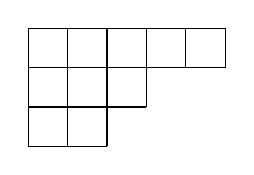
\begin{tikzpicture}
        \begin{scope}[scale=0.5]
            \draw (0, 3) -- (5, 3); \draw (0, 2) -- (5, 2); \draw (0, 1) -- (3, 1); \draw (0, 0) -- (2, 0); \draw (0, 3) -- (0, 0); \draw (1, 3) -- (1, 0); \draw (2, 3) -- (2, 0); \draw (3, 3) -- (3, 1); \draw (4, 3) -- (4, 2); \draw (5, 3) -- (5, 2);
        \end{scope}
    \end{tikzpicture} \]
    The \textit{arm length} of a box $s$, denoted $a_\lambda(s)$, is the number of boxes to the right of $s$. The \textit{leg length} of $s$, denoted $l_\lambda(s)$, is the number of boxes below $s$. The \textit{hook length} $s$ is $a_\lambda(s) + l_\lambda(s) + 1$.
    
    A \textbf{Young tableau} on a Young diagram is a numbering of the boxes by the integers $1, 2, \ldots, n$.
    % A Young tableau is \textbf{standard} if the entries in each row and each column are increasing.
\end{topic}

\begin{topic}{generating-function}{generating function}
    The \textbf{generating function} of a sequence $a_0, a_1, a_2, \ldots$ in a \tref{AA:ring}{commutative ring} $R$ is the formal power series
    \[ \sum_{n = 0}^{\infty} a_n t^n = a_0 + a_1 t + a_2 t^2 + \cdots \in R \llbracket t \rrbracket . \]
\end{topic}

\begin{example}{generating-function}
    \begin{itemize}
        \item The generating function of the constant sequence $1, 1, 1, \ldots$ is
        \[ \sum_{n = 0}^{\infty} t^n = \frac{1}{1 - t} . \]
        \item The generating function of the linear sequence $0, 1, 2, 3, \ldots$ is
        \[ \sum_{n = 0}^{\infty} n t^{n} = t \cdot \frac{d}{dt} \sum_{n = 0}^{\infty} t^{n} = t \cdot \frac{d}{dt} \left( \frac{1}{1 - t} \right) = \frac{t}{(1 - t)^2} . \]
        % \item The generating function of 
    \end{itemize}
\end{example}

\begin{example}{generating-function}
    Assuming $R$ has \tref{AA:characteristic}{characteristic} zero, the sequence can be obtained from the generating function $F \in R \llbracket t \rrbracket$ as follows. Writing
    \[ F = \sum_{n = 0}^{\infty} a_n t^n = a_0 + a_1 t + a_2 t^2 + \cdots , \]
    we obtain the coefficients $a_n$ from the $n$-th derivatives of $F$ as
    \[ a_n = \frac{F^{(n)}(0)}{n!} . \]
\end{example}

\begin{topic}{mobius-function}{Möbius function}
    The \textbf{Möbius function} $\mu$ is the function that assigns to any positive integer $n > 0$ the value
    \[ \mu(n) = \sum_{\substack{1 \le k \le n \\ \gcd(k, n) = 1}} e^{2\pi i \frac{k}{n}} , \]
    or alternatively,
    \[ \mu(n) = \left\{ \begin{array}{cl}
         +1 & \textup{ if $n$ is square-free with even number of prime factors}, \\
         -1 & \textup{ if $n$ is square-free with odd number of prime factors}, \\
         0 & \textup{ if $n$ has a squared prime factor}.
    \end{array} \right. \]
\end{topic}

\begin{example}{mobius-function}
    The first few values of $\mu$ are given by
    \[ \begin{array}{lllll}
        \mu(1) = 1, & \mu(2) = -1, & \mu(3) = -1, & \mu(4) = 0, & \mu(5) = -1, \\
        \mu(6) = 1, & \mu(7) = -1, & \mu(8) = 0, & \mu(9) = 0, & \mu(10) = 1, \ldots
    \end{array} \]
\end{example}

\begin{topic}{cantor-theorem}{Cantor's theorem}
    \textbf{Cantor's theorem} states that the cardinality of a set $A$ is always strictly smaller than the cardinality of its power set $\mathcal{P}(A)$.
\end{topic}

\begin{example}{cantor-theorem}
    \begin{proof}
        The cardinality of $A$ is at most the cardinality of $\mathcal{P}(A)$ since $x \mapsto \{ x \}$ is an injection $A \to \mathcal{P}(A)$.
        Conversely, suppose that there exists a surjective function $f : A \to \mathcal{P}(A)$, and let $B = \{ x \in A \mid x \not\in f(x) \}$. Then by surjectivity of $f$ there exists some $y \in A$ such that $f(y) = B$. But then $y \in B$ if and only if $y \not\in f(y) = B$, which is a contradiction. Therefore, the cardinality of $A$ is strictly smaller than that of $\mathcal{P}(A)$.
    \end{proof}
\end{example}

\begin{topic}{schur-function}{Schur function}
    Let $n$ be a positive integer. Write $a_\alpha = \det(x_i^{\alpha_j})_{i, j = 1}^{n}$ for any sequence $\alpha = (\alpha_1, \ldots, \alpha_n)$. For any partition $\lambda = (\lambda_1, \ldots, \lambda_n)$ of length at most $n$, the \textbf{Schur polynomial} of $\lambda$ is the \tref{AA:symmetric-polynomial}{polynomial}
    \[ s_\lambda = a_{\lambda + \delta} / a_\delta \in \ZZ[x_1, \ldots, x_n] , \]
    where $\delta = (n - 1, n - 2, \ldots, 1, 0)$.
    
    In passing from $n$ to $n + 1$, it can be seen that $s_\lambda(x_1, x_2, \ldots, x_n, 0) = s_\lambda(x_1, x_2, \ldots, x_n)$. Hence, there is a uniquely defined element
    \[ s_\lambda \in \Lambda := \bigoplus_{r \ge 0} \Lambda^r , \quad \textup{ where  } \Lambda^r = \varprojlim_n \ZZ[x_1, \ldots, x_n]_{(r)}^{S_n} , \]
    called the \textbf{Schur function} of $\lambda$.
\end{topic}

\begin{example}{schur-function}
    For $n = 3$, we have
    \begin{itemize}
        \item $s_{(0, 0, 0)} = 1$,
        \item $s_{(1, 0, 0)} = x_1 + x_2 + x_3$,
        \item $s_{(1, 1, 0)} = x_1 x_2 + x_1 x_3 + x_2 x_3$,
        \item $s_{(1, 1, 1)} = x_1 x_2 x_3$,
        \item $s_{(2, 0, 0)} = x_1^2 + x_1 x_2 + x_1 x_3 + x_2^2 + x_2 x_3 + x_3^2$,
        \item $s_{(2, 1, 0)} = (x_1 + x_2) (x_1 + x_3) (x_2 + x_3)$.
    \end{itemize}
    For any $n \ge 1$ and $\lambda = (1, 0, 0, \ldots)$, we have $s_\lambda = \sum_{i = 1}^{n} x_i$, so we obtain the Schur function $s_\lambda = \sum_{i = 1}^{\infty} x_i \in \Lambda$.
\end{example}

% \begin{topic}{macdonald-polynomials}{Macdonald polynomials}
%     Let $q$ and $t$ be two parameters.
    
%     The \textbf{Macdonald polynomials} are a family of polynomials $P_\lambda(q, t)$ uniquely determined by the conditions
%     \[ P_\lambda(q, t) = m_\lambda + \sum_{\mu < \lambda} m_\mu \]
%     \[ \langle P_\lambda, P_\mu \rangle_{q, t} = 0 \quad \textup{ for } \lambda \ne \mu . \]
%     where
%     \[ \langle p_\lambda, p_\mu \rangle = \delta_{\lambda \mu} z_\lambda \prod_{i = 1}^{\ell(\lambda)} \frac{1 - q^{\lambda_i}}{1 - t^{\lambda_i}} . \]
% \end{topic}

\begin{topic}{hall-inner-product}{Hall inner product}
    Let $\Lambda$ be the ring of symmetric polynomials in infinitely many variables. For any \tref{GM:integer-partition}{partition} $\lambda = (\lambda_1, \ldots, \lambda_n)$, let $m_\lambda \in \Lambda$ and $h_\lambda \in \Lambda$ denote the \tref{AA:symmetric-polynomial}{monomial and homogeneous symmetric polynomials} in infinitely many variables, respectively. It can be shown that both $\{ m_\lambda \}$ and $\{ h_\lambda \}$ form a $\ZZ$-basis of $\Lambda$.
    
    The \textbf{Hall inner product} is the symmetric bilinear map given by
    \[ \langle \cdot, \cdot \rangle : \Lambda \times \Lambda \to \Lambda, \qquad \langle m_\lambda, h_\mu \rangle = \delta_{\lambda \mu} . \]
\end{topic}

\begin{example}{hall-inner-product}
    The \tref{schur-function}{Schur functions} $\{ s_\lambda \}$ also form a $\ZZ$-basis for $\Lambda$, and moreover, an orthogonal $\ZZ$-basis:
    \[ \langle s_\lambda, s_\mu \rangle = \delta_{\lambda \mu} \quad \textup{ for all } \lambda, \mu . \]
\end{example}

\begin{topic}{binomial-theorem}{binomial theorem}
    Let $R$ be a \tref{AA:ring}{commutative ring $R$}. The \textbf{binomial theorem} states that
    \[ (x + y)^n = \sum_{k = 0}^{n} \binom{n}{k} x^{n - k} y^k \]
    for all $x, y \in R$ and any integer $n \ge 0$.
\end{topic}

\begin{topic}{integer-partition}{integer partition}
    A \textbf{partition} of a non-negative integer $n$ is a tuple of integers $\lambda = (\lambda_1, \ldots, \lambda_k)$ such that $\lambda_1 + \cdots + \lambda_k = n$ and $\lambda_1 \ge \cdots \ge \lambda_k \ge 0$.
\end{topic}

\begin{example}{integer-partition}
    There are $7$ partitions of $5$:
    \begin{itemize}
        \item $5 = 1 + 1 + 1 + 1 + 1$,
        \item $5 = 2 + 1 + 1 + 1$,
        \item $5 = 2 + 2 + 1$,
        \item $5 = 3 + 1 + 1$,
        \item $5 = 3 + 2$,
        \item $5 = 4 + 1$,
        \item $5 = 5$.
    \end{itemize}
\end{example}

\begin{topic}{conjugate-partition}{conjugate partition}
    Given a \tref{integer-partition}{partition} $\lambda = (\lambda_1, \ldots, \lambda_k)$ of a non-negative integer $n$, the \textbf{conjugate partition} $\lambda' = (\lambda'_1, \ldots, \lambda'_\ell)$ to $\lambda$ is given by
    \[ \lambda'_i = | \{ 1 \le j \le k \mid \lambda_j \ge i \} | \]
    for $1 \le i \le \ell$, where $\ell = \lambda_1$.
\end{topic}

\begin{example}{conjugate-partition}
    The conjugate partition to $\lambda = (5, 3, 2)$ is $\lambda' = (3, 3, 2, 1, 1)$. Note that the \tref{young-diagram}{Young diagram} corresponding to a conjugate partition $\lambda'$ is the transpose of the Young diagram corresponding to $\lambda$.
    \[ 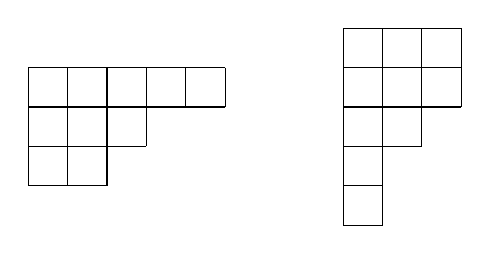
\begin{tikzpicture}
        \begin{scope}[scale=0.5]
            \draw (0, 3) -- (5, 3); \draw (0, 2) -- (5, 2); \draw (0, 1) -- (3, 1); \draw (0, 0) -- (2, 0); \draw (0, 3) -- (0, 0); \draw (1, 3) -- (1, 0); \draw (2, 3) -- (2, 0); \draw (3, 3) -- (3, 1); \draw (4, 3) -- (4, 2); \draw (5, 3) -- (5, 2);
        \end{scope}
        \begin{scope}[scale=0.5, shift={(8, -1)}]
            \draw (0, 5) -- (3, 5); \draw (0, 4) -- (3, 4); \draw (0, 3) -- (3, 3); \draw (0, 2) -- (2, 2); \draw (0, 1) -- (1, 1); \draw (0, 0) -- (1, 0); \draw (0, 0) -- (0, 5); \draw (1, 0) -- (1, 5); \draw (2, 2) -- (2, 5); \draw (3, 3) -- (3, 5);
        \end{scope}
    \end{tikzpicture}\]
\end{example}

\begin{topic}{zorns-lemma}{Zorn's lemma}
    Let $P$ be a partially ordered set, such that every chain in $P$
    \[ x_1 \le x_2 \le x_3 \le \cdots \]
    has an upper bound in $P$. Then \textbf{Zorn's lemma} states that $P$ contains at least one maximal element.
\end{topic}

\begin{topic}{filter}{filter}
    Let $(P, \le)$ be a partially ordered set. A \textbf{filter} on $P$ is a subset $F \subset P$ such that
    \begin{itemize}
        \item (\textit{non-empty}) $F$ is non-empty,
        \item (\textit{downward directed}) for every $x, y \in F$ there exists some $z \in F$ with $z \le x$ and $z \le y$,
        \item (\textit{upward-closed}) for all $x \in F$ and $y \in P$ with $x \le y$, also $y \in F$.
    \end{itemize}
\end{topic}

\begin{example}{filter}
    Let $X$ be a \tref{TO:topological-space}{topological space}, and $x \in X$ a point. The \textit{neighborhood filter} of $x$, denoted $\mathcal{N}_x$, is the filter consisting of all \tref{TO:neighborhood}{neighborhoods} of $x$. It is a filter on the set of all subsets of $X$, partially ordered by inclusion.
\end{example}

\begin{topic}{fermat-little-theorem}{Fermat's little theorem}
    Let $p$ be a prime number and $a$ an integer. \textbf{Fermat's little theorem} states that
    \[ a^p \equiv a \mod p . \]
\end{topic}

\begin{example}{fermat-little-theorem}
    \begin{proof}
        For $a \equiv 0 \mod p$ the proof is trivial. Otherwise, the order of $a \mod p \in (\ZZ/p\ZZ)^*$ divides the order of the group, which is $p - 1$, so it follows that $a^{p - 1} \equiv 1 \mod p$, and hence $a^p \equiv a \mod p$.
    \end{proof}
\end{example}


\chapter{Set Theory}
\renewcommand{\cat}{ST}
\begin{topic}{power-set}{power set}
    The \textbf{power set} of a set $A$ is the set of all subsets of $A$,
    \[ P(A) = \{ B \mid B \subset A \} . \]
\end{topic}

\begin{topic}{cantor-theorem}{Cantor's theorem}
    \textbf{Cantor's theorem} states that for any set $A$, there does not exist a surjective function from $A$ to the \tref{power-set}{power set} $P(A)$ of $A$.
\end{topic}

\begin{example}{cantor-theorem}
    \begin{proof}
        Suppose for a contradiction that $f : A \to P(A)$ is a surjective function, and let $S = \{ x \in A \mid x \not\in f(x) \}$. Since $f$ is surjective, there exists some $x \in A$ with $f(x) = S$. But now, by definition of $S$,
        \[ x \in S \iff x \not\in f(x) = S , \]
        which is a contradiction.
    \end{proof}
\end{example}

\begin{topic}{axiom-of-choice}{axiom of choice}
    The \textbf{axiom of choice} states that for every set $X$ of non-empty sets, there exists a function
    \[ f : X \to \bigcup_{A \in X} A \]
    such that $f(A) \in A$ for all $A \in X$.
\end{topic}

\begin{topic}{cantor-set}{Cantor set}
    The \textbf{Cantor set} is the set
    \[ C = \bigcap_{n = 0}^{\infty} C_n , \]
    where $C_0 = [0, 1]$ and $C_n = \frac{1}{3} \left( C_{n - 1} \cup (2 + C_{n - 1}) \right)$ for any $n \ge 1$.
\end{topic}

\begin{topic}{partially-ordered-set}{partially ordered set}
    A \textbf{partial order} on a set $P$ is a \tref{binary-relation}{binary relation} $\le$ on $P$ such that
    \begin{itemize}
        \item (\textit{reflexivity}) $x \le x$ for all $x \in P$,
        \item (\textit{anti-symmetry}) if $x \le y$ and $y \le x$ then $x = y$ for all $x, y \in P$,
        \item (\textit{transitivity}) if $x \le y$ and $y \le z$ then $x \le z$ for all $x, y, z \in P$.
    \end{itemize}
    A \textbf{partially ordered set} is a set $P$ together with a partial order $\le$.
\end{topic}

\begin{topic}{lattice}{lattice}
    A \textbf{lattice} is a \tref{partially-ordered-set}{partially ordered set} $(P, \le)$ such that
    \begin{itemize}
        \item (\textit{least upper bound}) any two elements $x, y \in P$ have a least upper bound $x \vee y$,
        \item (\textit{greatest lower bound}) any two elements $x, y \in P$ have a greatest lower bound $x \wedge y$,
        \item (\textit{least element}) there exists a least element $0 \in P$,
        \item (\textit{greatest element}) there exists a greatest element $1 \in P$.
    \end{itemize}
\end{topic}

\begin{topic}{boolean-algebra}{Boolean algebra}
    A \textbf{Boolean algebra} is a \tref{lattice}{lattice} $(P, \le)$ such that
    \begin{itemize}
        \item (\textit{complements}) for every $x \in P$ there exists an element $\neg x \in P$ such that $x \vee \neg x = 1$ and $x \wedge \neg x = 0$,
        \item (\textit{distributivity}) $x \wedge (y \vee z) = (x \wedge y) \vee (x \wedge z)$ for all $x, y, z \in P$.
    \end{itemize}
    A Boolean algebra $(P, \le)$ is \textbf{complete} if every subset $A \subset P$ has a least upper bound and a greatest lower bound.
\end{topic}

\begin{example}{boolean-algebra}
    Let $X$ be a set, and let $P$ be the \tref{power-set}{power set} of $X$. Then $(P, \subset)$ is a Boolean algebra, where the negation $\neg A$ is the difference $X \setminus A$.
\end{example}

\begin{topic}{atom}{atom}
    Let $(P, \le)$ be a \tref{partially-ordered-set}{partially ordered set} with a least element $0 \in P$. An \textbf{atom} in $P$ is an element $x \in P$ not equal to $0$ such that $y \le x$ implies $y = 0$ or $y = x$ for all $y \in P$.
\end{topic}

\begin{topic}{heyting-algebra}{Heyting algebra}
    A \textbf{Heyting algebra} is a \tref{lattice}{lattice} $(H, \le, \vee, \wedge, 0, 1)$ together with a binary operation $\rightarrow$, called \textit{Heyting implication}, such that $x \wedge y \le z$ if and only if $x \le y \rightarrow z$ for all $x, y, z \in H$.
\end{topic}

\begin{topic}{binary-relation}{binary relation}
    A \textbf{binary relation} $R$ over two sets $X$ and $Y$ is a subset of the product $X \times Y$.
    
    Usually, one writes $x R y$ to mean $(x, y) \in R$.
\end{topic}

\begin{topic}{filter}{filter}
    Let $(P, \le)$ be a \tref{partially-ordered-set}{partially ordered set}. A \textbf{filter} on $P$ is a subset $F \subset P$ such that
    \begin{itemize}
        \item (\textit{non-empty}) $F$ is non-empty,
        \item (\textit{downward directed}) for every $x, y \in F$ there exists some $z \in F$ with $z \le x$ and $z \le y$,
        \item (\textit{upward-closed}) for all $x \in F$ and $y \in P$ with $x \le y$, also $y \in F$.
    \end{itemize}
\end{topic}

\begin{example}{filter}
    Let $X$ be a \tref{TO:topological-space}{topological space}, and $x \in X$ a point. The \textit{neighborhood filter} of $x$, denoted $\mathcal{N}_x$, is the filter consisting of all \tref{TO:neighborhood}{neighborhoods} of $x$. It is a filter on the set of all subsets of $X$, partially ordered by inclusion.
\end{example}

\begin{topic}{de-morgan-laws}{De Morgan's laws}
    Let $B$ be a \tref{boolean-algebra}{Boolean algebra}. \textbf{De Morgan's laws} state that
    \[ \neg (x \lor y) = \neg x \land \neg y \quad \textup{ and } \quad \neg (x \land y) = \neg x \lor \neg y \]
    for all $x, y \in B$.
\end{topic}


\chapter{Linear Algebra}
\renewcommand{\cat}{LA}
\begin{topic}{vector-space}{vector space}
    A \textbf{vector space} over a \tref{AA:field}{field} $k$ is a \tref{AA:module}{$k$-module}. Its elements are called \textit{vectors}.
    Concretely, a vector space over $k$ is a set $V$ with a distinguished object $0 \in V$ and two operations
    \[ + : V \times V \to V, \quad \cdot : k \times V \to V \]
    satisfying
    \begin{itemize}
        \item (\textit{commutativity}) $x + y = y + x$ for all $x, y \in V$,
        \item (\textit{associativity}) $(x + y) + z = x + (y + z)$ for all $x, y, z \in V$,
        \item (\textit{zero vector}) $x + 0 = x = 0 + x$ for all $x \in V$,
        \item (\textit{negatives}) for all $x \in V$ there exists some $-x \in V$ such that $x + (-x) = 0$,
        \item (\textit{associativity}) $\lambda \cdot (\mu \cdot x) = (\lambda \mu) \cdot x$ for all $x \in V$ and $\lambda, \mu \in k$,
        \item (\textit{unit}) $1 \cdot x = x$ for all $x \in V$,
        \item (\textit{distributivity 1}) $\lambda \cdot (x + y) = (\lambda \cdot x) + (\lambda \cdot y)$ for all $x, y \in V$ and $\lambda \in k$,
        \item (\textit{distributivity 2}) $(\lambda + \mu) \cdot x = (\lambda \cdot x) + (\mu \cdot x)$ for all $x \in V$ and $\lambda, \mu \in k$.
    \end{itemize}
\end{topic}

\begin{topic}{linear-subspace}{linear subspace}
    Let $V$ be a \tref{vector-space}{vector space} over a field $k$. A \textbf{linear subspace} of $V$ is a subset $W \subset V$ which is closed under addition and scalar multiplication: $w_1 + w_2 \in W$ for all $w_1, w_2 \in W$ and $\lambda w \in W$ for all $w \in W$ and $\lambda \in k$.
\end{topic}

\begin{topic}{linearly-independent}{linearly independent}
    Let $V$ be a \tref{vector-space}{vector space}. A set of vectors $S \subset V$ is said to be \textbf{linearly independent} if for any relation
    \[ \sum_{i = 1}^{n} a_i v_i = 0, \qquad \textup{with $v_i \in S$ distinct and $a_i \in k$,} \]
    it follows that $a_1 = \ldots = a_n = 0$.
\end{topic}

\begin{topic}{span}{span}
    Let $V$ be a \tref{vector-space}{vector space}, and $S \subset V$ a subset. The \textbf{span} of $S$ is the \tref{linear-subspace}{subspace} of all linear combinations of vectors in $S$.
    \[ \textup{span}(S) = \left\{ \sum_{i = 1}^{n} a_i v_i \textup{ for any } v_i \in S \textup{ and } a_i \in k \right\} \]
\end{topic}

\begin{topic}{basis}{basis}
    Let $V$ be a \tref{vector-space}{vector space}. A set of vectors in $V$ is a \textbf{basis} for $V$ if it \tref{span}{spans} $V$ and is \tref{linearly-independent}{linearly independent}.
    
    Equivalently, a set is a basis if each vector in $V$ can be expressed uniquely as a linear combination of vectors in the set.
\end{topic}

\begin{topic}{dimension}{dimension}
    Let $V$ be a \tref{vector-space}{vector space}. The \textbf{dimension} of $V$ is the cardinality of any \tref{basis}{basis} of $V$. It is often denoted by $\dim(V)$.
\end{topic}

\begin{topic}{linear-map}{linear map}
    A \textbf{linear map} is a map $f : V \to W$ between \tref{vector-space}{vector spaces} such that
    \begin{itemize}
        \item $f(u + v) = f(u) + f(v)$,
        \item $f(\lambda v) = \lambda f(v)$,
    \end{itemize}
    for all vectors $u, v \in V$ and scalars $\lambda \in k$.
\end{topic}

\begin{topic}{matrix}{matrix}
    Let $V$ and $W$ be finite-dimensional \tref{vector-space}{vector spaces}, and $f : V \to W$ a \tref{linear-map}{linear map}. If $(v_1, v_2, \ldots, v_n)$ and $(w_1, w_2, \ldots, w_m)$ are ordered \tref{basis}{bases} of $V$ and $W$, respectively, then the \textbf{matrix} associated to $f$ is the $m \times n$ matrix
    \[ A = \begin{pmatrix} a_{11} & a_{21} & \cdots & a_{n1} \\ a_{21} & a_{22} & \cdots & a_{2n} \\ \vdots & \vdots & \ddots & \vdots \\ a_{m1} & a_{m2} & \cdots & a_{mn} \end{pmatrix} \]
    where $a_{ij}$ is the $i$-th component of $f(v_j)$ with respect to the basis for $W$.
\end{topic}

\begin{topic}{matrix-multiplication}{matrix multiplication}
    Let $A = (a_{ij})$ be an $m \times n$ matrix, and $B = (b_{ij})$ be an $n \times \ell$ matrix. The \textbf{matrix product} $AB$ is the $m \times \ell$ matrix $C = (c_{ij})$ given by
    \[  c_{ij} = \sum_{k = 1}^{n} a_{ik} b_{kj} . \]
\end{topic}

\begin{topic}{matrix-transpose}{matrix transpose}
    The \textbf{transpose} of a matrix $A = (a_{ij})$ is the matrix $A^T = (b_{ij})$ given by $b_{ij} = a_{ji}$.
\end{topic}

% \begin{topic}{row-echelon-form}{(reduced) row-echelon form}
    
% \end{topic}

\begin{topic}{invertible-matrix}{invertible matrix}
    An $n \times n$ matrix $A$ is \textbf{invertible} if there exists an $n \times n$ matrix $B$ such that $AB = BA = I$. In this case, $B$ is called the \textbf{inverse} of $A$, and is the unique matrix with this property.
    
    If $A$ is not invertible, it is called \textbf{singular}.
\end{topic}

\begin{example}{invertible-matrix}
    When $n = 2$, we have
    \[ \begin{pmatrix} a & b \\ c & d \end{pmatrix} = \frac{1}{ad - bc} \begin{pmatrix} d & -b \\ -c & a \end{pmatrix} . \]
\end{example}

\begin{topic}{matrix-rank}{matrix rank}
    The \textbf{rank} of an $m \times n$ matrix $A$ the \tref{dimension}{dimension} of its \textit{row space} $\im A$.
\end{topic}

\begin{topic}{kernel}{kernel}
    The \textbf{kernel}, or \textbf{nullspace}, of a \tref{linear-map}{linear transformation} $T : V \to W$ is the subspace
    \[ \ker T = \left\{ v \in V : T(v) = 0 \right\} \subset V . \]
\end{topic}

\begin{topic}{projection}{projection}
    A \textbf{projection} is a \tref{linear-map}{linear transformation} $P : V \to V$ with $P^2 = P$.
\end{topic}

\begin{topic}{determinant}{determinant}
    The \textbf{determinant} of an $n \times n$ matrix $A$ is the scalar given by
    \[ \det(A) = \sum_{\sigma \in S_n} \left( \textup{sign}(\sigma) \prod_{i = 1}^{n} a_{i, \sigma(i)} \right) , \]
    where $\textup{sign}(\sigma)$ denotes the \tref{GT:permutation-sign}{sign} of the \tref{GT:symmetric-group}{permutation} $\sigma \in S_n$. The determinant has the property that $A$ is \tref{invertible-matrix}{invertible} if and only if $\det(A) \ne 0$.
    
    Alternatively, the determinant of $A$ is the scalar corresponding to the map induced on the top exterior power of $V$,
    \[ \wedge^n A : \wedge^n V \to \wedge^n V . \]
\end{topic}

\begin{example}{determinant}
    When $n = 2$,
    \[ \det \begin{pmatrix} a & b \\ c & d \end{pmatrix} = ad - bc . \]
    When $n = 3$,
    \[ \det \begin{pmatrix} a & b & c \\ d & e & f \\ g & h & i \end{pmatrix} = a(ei - fh) - b(di - fg) + c(dh - eg) . \]
\end{example}

\begin{topic}{trace}{trace}
    The \textbf{trace} of an $n \times n$ matrix $A$ is the sum of its diagonal entries,
    \[ \operatorname{tr}(A) = \sum_{i = 1}^{n} a_{ii} . \]
\end{topic}

\begin{example}{trace}
    The trace is cyclic in the sense that for any $A, B \in \textup{Mat}_{n \times n}(k)$ it holds that
    \[ \operatorname{tr}(AB) = \sum_{i, j = 1}^{n} A_{ij} B_{ji} = \sum_{i, j = 1}^{n} B_{ji} A_{ij} = \operatorname{tr}(BA) . \]
\end{example}

\begin{topic}{cofactor-matrix}{cofactor matrix}
    Let $A = (a_{ij})$ be an $n \times n$ matrix. The \textbf{cofactor} of an entry $a_{ij}$ of $A$ is
    \[ a'_{ij} = (-1)^{i + j} \det(A_{ij}), \]
    where $A_{ij}$ is the matrix obtained from $A$ by removing the $i$-th row and $j$-th column. The \textbf{cofactor matrix} of $A$ is then the $n \times n$ matrix $A' = (a'_{ij})$.
\end{topic}

\begin{topic}{adjoint-matrix}{adjoint matrix}
    Let $A$ be an $n \times n$ matrix. The \textbf{adjoint} of $A$ is the \tref{matrix-transpose}{transpose} of its \tref{cofactor-matrix}{cofactor matrix}:
    \[ \textup{adj}(A) = (A')^T . \]
    It has the property that
    \[ \textup{adj}(A) A = \det(A) I , \]
    so in particular, when $\det(A) \ne 0$, one has
    \[ A^{-1} = \frac{1}{\det(A)} \textup{adj}(A) . \]
\end{topic}

\begin{topic}{eigenvalue}{eigenvalue/eigenvector}
    Let $A : V \to V$ be a \tref{linear-map}{linear map}. A scalar $\lambda$ is an \textbf{eigenvalue} of $A$ if there exists a nonzero vector $v \in V$ such that $A v = \lambda v$. The vector $v$ is then an \textbf{eigenvector} of $A$ corresponding to $\lambda$.
\end{topic}

\begin{topic}{characteristic-polynomial}{characteristic polynomial}
    Let $A$ be an $n \times n$ matrix. The \textbf{characteristic polynomial} of $A$ is the polynomial of degree $n$ given by
    \[ p_A(\lambda) = \det(\lambda I - A) . \]
    Its roots are precisely the \tref{eigenvalue}{eigenvalues} of $A$.
\end{topic}

\begin{example}{characteristic-polynomial}
    The coefficients of the characteristic polynomial are given by
    \[ p_A(\lambda) = \sum_{k = 0}^{n} \lambda^{n - k} (-1)^k \textup{tr}(\wedge^k A) , \]
    where $\wedge^k A : \wedge^k k^n \to \wedge^k k^n$ is the \tref{AA:exterior-algebra}{$k$-th exterior power} of $A$.
    In particular, the constant coefficient is the \tref{determinant}{determinant} of $A$.
\end{example}

\begin{topic}{diagonalization}{diagonalization}
    A \textbf{diagonalization} of an $n \times n$ matrix $A$ consists of an \tref{invertible-matrix}{invertible matrix} $C$ and a diagonal matrix $D$ such that
    \[ D = C A C^{-1} . \]
    If such a diagonalization exists, $A$ is said to be \textbf{diagonalizable}.
\end{topic}

\begin{example}{diagonalization}
    Let $A$ be a diagonalizable matrix. Note that we can write
    \[ AC = DC , \]
    with $C$ invertible and $D$ diagonal. From this expression it is clear that the columns of $C$ must be \tref{eigenvalue}{eigenvectors} of $A$, and that $D$ contains the corresponding eigenvalues. The matrix $C$ being invertible means that $A$ has $n$ linearly independent eigenvectors.
\end{example}

\begin{topic}{algebraic-geometric-multiplicity}{algebraic/geometric multiplicity}
    Let $A$ be an $n \times n$ matrix. The \textbf{algebraic multiplicity} of an eigenvalue $\lambda$ of $A$ is its multiplicity as a root of the \tref{characteristic-polynomial}{characteristic polynomial} of $A$.
    
    The \textbf{geometric multiplicity} is the \tref{dimension}{dimension} of the corresponding \textit{eigenspace}
    \[ E_\lambda(A) = \{ v \in V \mid A v = \lambda v \} . \]
\end{topic}

\begin{example}{algebraic-geometric-multiplicity}
    Consider the matrix
    \[ A = \begin{pmatrix} 2 & 1 & 0 \\ 0 & 2 & 0 \\ 0 & 0 & 3 \end{pmatrix} . \]
    Its characteristic polynomial is $p_A(\lambda) = (2 - \lambda)^2 (3 - \lambda)$, so its eigenvalues are $\lambda = 2$ (with alg. multiplicity $2$) and $\lambda = 3$ (with alg. multiplicity $1$). However, both have a geometric multiplicity of $1$ as
    \[ E_2 = \ker(A - 2I) = \textup{span}(1, 0, 0) \quad \textup{ and } \quad E_3 = \ker(A - 3I) = \textup{span}(0, 0, 1) . \]
\end{example}

\begin{topic}{dual-vector-space}{dual vector space}
    Given a \tref{vector-space}{vector space} $V$, the \textbf{dual vector space} $V^*$ is defined as the vector space of all \tref{linear-map}{linear maps} $f : V \to k$.
\end{topic}

\begin{example}{dual-vector-space}
    For any vector space $V$, there is a canonical linear map from $V$ to the double dual $V^{**}$ given by
    \[ V \to V^{**}, \quad v \mapsto (f \mapsto f(v)) . \tag{$(*)$} \]
    This map is injective since $f(v) = 0$ for all $f \in V^*$ implies $v = 0$. For finite-dimensional $V$ this map is also surjective. Namely, let $e_1, \ldots, e_n$ be a basis for $V$, then $f_1, \ldots, f_n \in V^*$ given by $f_i(e_j) = \delta_{ij}$ form a basis for $V^*$. Now for any $\varphi \in V^{**}$, the element
    \[ v = \sum_{i = 1}^{n} \varphi(f_i) e_i \]
    maps under $(*)$ to $\varphi$. In particular, $V^{**}$ is canonically isomorphic to $V$.
    
    If $V$ is not finite-dimensional, the map $(*)$ need not be surjective. Namely, let $V$ be a vector space with an infinite basis $e_1, e_2, \ldots$, and define $f_1, f_2, \ldots \in V^*$ by $f_i(e_j) = \delta_{ij}$. Furthermore, take $\varphi \in V^{**}$ to be any map such that $\varphi(f_i) = 1$. Since any $v \in V$ can be written as a finite sum $v = \sum_{i = 1}^{N} v_i e_i$, we have $f_{N + 1}(v) = 0 \ne 1 = \varphi(f_{N + 1})$, which shows that $(*)$ is not surjective.
\end{example}

\begin{topic}{grassmannian}{Grassmannian}
    Given a \tref{LA:vector-space}{vector space} $V$, and $r \ge 0$, the \textbf{Grassmannian} $\textup{Gr}(r, V)$ is a space that parametrizes all $r$-dimensional \tref{linear-subspace}{linear subspaces} of $V$.
\end{topic}

\begin{example}{grassmannian}
    When $r = 1$, the Grassmanian $\textup{Gr}(1, V)$ parametrizes all lines in $V$ through the origin, that is, $\textup{Gr}(1, V) = \PP(V)$.
\end{example}

\begin{topic}{general-linear-group}{general linear group}
    The \textbf{general linear group} of degree $n$ over a field $k$, denoted $\textup{GL}_n(k)$, is the \tref{GT:group}{group} of $n \times n$ \tref{invertible-matrix}{invertible matrices} with the operation of matrix multiplication.
\end{topic}

\begin{topic}{special-linear-group}{special linear group}
    The \textbf{special linear group} of degree $n$ over a field $k$, denoted $\textup{SL}_n(k)$, is the \tref{GT:group}{group} of $n \times n$ \tref{invertible-matrix}{invertible matrices} with \tref{determinant}{determinant} $1$, with the operation of matrix multiplication.
\end{topic}

\begin{topic}{orthogonal-matrix}{orthogonal matrix}
    An $n \times n$ matrix $A$ is \textbf{orthogonal} if $A A^T = I$, where $A^T$ denotes the \tref{matrix-transpose}{transpose} of $A$.
\end{topic}

\begin{topic}{orthogonal-group}{(special) orthogonal group}
    The \textbf{orthogonal group} of degree $n$ over a field $k$, denoted $\textup{O}(n, k)$, is the \tref{GT:group}{group} of $n \times n$ \tref{orthogonal-matrix}{orthogonal matrices} with the operation of matrix multiplication.
    
    The \textbf{special orthogonal group} is the \tref{GT:subgroup}{subgroup} $\textup{SO}(n, k) \subset \textup{O}(n, k)$ of matrices with \tref{determinant}{determinant} $1$.
\end{topic}

\begin{topic}{unitary-matrix}{unitary matrix}
    An $n \times n$ matrix $U$ over $\CC$ is \textbf{unitary} if $UU^H = I$, where $U^H$ is its conjugate \tref{matrix-transpose}{transpose}.
\end{topic}

\begin{topic}{unitary-group}{(special) unitary group}
    The \textbf{unitary group} of degree $n$, denoted $\textup{U}(n)$, is the \tref{GT:group}{group} of $n \times n$ \tref{unitary-matrix}{unitary matrices} with the operation of matrix multiplication.
    
    The \textbf{special unitary group} is the \tref{GT:subgroup}{subgroup} $\textup{SU}(n) \subset \textup{U}(n)$ of matrices with \tref{determinant}{determinant} $1$.
\end{topic}

\begin{topic}{symplectic-matrix}{symplectic matrix}
    A $2n \times 2n$ matrix $M$ is \textbf{symplectic} if $M^T \Omega M = \Omega$, where $\Omega = \begin{pmatrix} 0 & I_n \\ -I_n & 0 \end{pmatrix}$.
\end{topic}

\begin{topic}{symplectic-group}{symplectic group}
    The \textbf{symplectic group} of degree $2n$ over a field $k$, denoted $\textup{Sp}_{2n}(k)$, is the \tref{GT:group}{group} of $2n \times 2n$ \tref{symplectic-matrix}{symplectic matrices} with the operation of matrix multiplication.
\end{topic}

\begin{topic}{hermitian-matrix}{Hermitian matrix}
    An $n \times n$ complex matrix $A$ is \textbf{Hermitian} if it is equal to its conjugate \tref{matrix-transpose}{transpose}, that is $A = A^H$.
\end{topic}

\begin{example}{hermitian-matrix}
    A Hermitian matrix $A$ always has real eigenvalues. Namely, if $Av = \lambda v$, then
    \[ \lambda \norm{v} = v^H A v = v^H A^H v = (A v)^H v = \overline{\lambda} v^H v = \overline{\lambda} \norm{v} , \]
    which shows $\lambda$ is real.
    
    Moreover, if $\lambda$ and $\mu$ are distinct eigenvalues, with respective eigenvectors $v$ and $w$, then $v$ and $w$ are orthogonal. Namely,
    \[ \mu \langle v^H, w \rangle = \langle v^H, A w \rangle = \langle v^H A^H, w \rangle = \lambda \rangle v^H, w \rangle , \]
    which shows $\langle v^H, w \rangle = 0$ as $\lambda - \mu \ne 0$.
\end{example}

\begin{topic}{pin-group}{pin group}
    The \textbf{pin group} $\textup{Pin}(V, q)$ of a \tref{vector-space}{vector space} $V$ over $k$ with a \tref{quadratic-form}{quadratic form} $q : V \to k$ is the subgroup of the units of the \tref{clifford-algebra}{Clifford algebra} $\textup{Cl}(V, q)$ of elements of the form $v_1 v_2 \cdots v_k$ with $q(v_i) = 1$.
    
    As a special case, $\textup{Pin}(n) = \textup{Pin}(\RR^n, \langle \cdot, \cdot \rangle)$.
\end{topic}

\begin{topic}{spin-group}{spin group}
    The \textbf{spin group} $\textup{Spin}(V, q)$ of a \tref{vector-space}{vector space} $V$ over $k$ with a \tref{quadratic-form}{quadratic form} $q : V \to k$ is the subgroup of the units of the \tref{clifford-algebra}{Clifford algebra} $\textup{Cl}(V, q)$ of elements of the form $v_1 v_2 \cdots v_{2k}$ with $q(v_i) = 1$.

    As a special case, $\textup{Spin}(n) = \textup{Spin}(\RR^n, \langle \cdot, \cdot \rangle)$.
    
    The \textbf{spin group} $\textup{Spin}(n)$ is the universal (double) cover of the \tref{orthogonal-group}{special orthogonal group} $\textup{SO}(n)$.
\end{topic}

\begin{example}{spin-group}
    Let $\{ e_i \}$ be an orthonormal basis for $V$ w.r.t. $q$. Define an \textit{antiautomorphism} $t : \textup{Cl}(V, q) \to \textup{Cl}(V, q)$ by $(e_i e_j \cdots e_k)^t = e_k \cdots e_j e_i$ and extending linearly. Then define the automorphism $\alpha : \textup{Cl}(V, q) \to \textup{Cl}(V, q)$ by $\alpha(v) = -v$ for $v \in V$. Let $a^*$ denote $\alpha(a)^t$ for $a \in \textup{Cl}(V, q)$.
    
    With this notation, an explicit double cover of $\textup{O}(V, q)$ by $\textup{Pin}(V, q)$ is given by
    \[ \rho : \textup{Pin}(V, q) \to \textup{O}(V, q), \quad \rho(a) v = a v a^* . \]
    Restricting $\rho$ to $\textup{Spin}(V, q)$ gives a double cover of $\textup{SO}(V, q)$.
\end{example}

\begin{topic}{clifford-algebra}{Clifford algebra}
    The \textbf{Clifford algebra} of a \tref{vector-space}{vector space} $V$ over a field $k$ with a \tref{quadratic-form}{quadratic form} $q : V \to k$ is the algebra over $k$ given by
    \[ \textup{Cl}(V, q) = T(V) / (v \otimes v - q(v)) , \]
    where $T(V)$ denotes the \tref{AA:tensor-algebra}{tensor algebra} of $V$.
\end{topic}

\begin{example}{clifford-algebra}
    Let $V$ be an $n$-dimensional vector space with basis vectors $e_1, \ldots, e_n$, which are orthogonal in the sense that $\langle e_i, e_j \rangle = \delta_{ij}$, where $\langle \cdot, \cdot \rangle$ is the bilinear form corresponding to the quadratic form $q$. Then $e_i \otimes e_i = q(e_i)$, and for $i \ne j$ we find
    \[ q(e_i) + q(e_j) = q(e_i + e_j) = (e_i + e_j) \otimes (e_i + e_j) = q(e_i) + e_i \otimes e_j + e_j \otimes e_i + q(e_j) , \]
    from which follows that $e_i \otimes e_j = - e_j \otimes e_i$. This shows that
    \[ \{ e_{i_1} \otimes e_{i_2} \otimes \cdots \otimes e_{i_k} : 1 \le i_1 < \cdots < i_k \le n \textup{ and } 0 \le k \le n  \} \]
    is a basis for $\textup{Cl}(V, q)$, and in particular
    \[ \dim_k \textup{Cl}(V, q) = \sum_{k = 0}^{n} \binom{n}{k} = 2^n . \]
\end{example}

\begin{example}{clifford-algebra}
    Let $V = \RR^4$ with quadratic form given by $q(t, x, y, z) = t^2 - x^2 - y^2 - z^2$. The corresponding Clifford algebra $\textup{Cl}_{1,3}(\RR)$ is generated (as an algebra) by the standard basis vectors $\gamma^0, \gamma^1, \gamma^2, \gamma^3$ satisfying
    \[ \{ \gamma^\mu, \gamma^\nu \} := \gamma^\mu \gamma^\nu + \gamma^\nu \gamma^\mu = 2 \eta^{\mu \nu} , \qquad \text{ where } \eta^{\mu \nu} = \begin{pmatrix} 1 & 0 & 0 & 0 \\ 0 & -1 & 0 & 0 \\ 0 & 0 & -1 & 0 \\ 0 & 0 & 0 & -1 \end{pmatrix} . \]
    This Clifford algebra can be represented as a matrix algebra, with
    \[
        \gamma^0 = \begin{pmatrix} 1 & 0 & 0 & 0 \\ 0 & 1 & 0 & 0 \\ 0 & 0 & -1 & 0 \\ 0 & 0 & 0 & -1 \end{pmatrix} , \quad
        \gamma^1 = \begin{pmatrix} 0 & 0 & 0 & 1 \\ 0 & 0 & 1 & 0 \\ 0 & -1 & 0 & 0 \\ -1 & 0 & 0 & 0 \end{pmatrix} , \]
    \[
        \gamma^2 = \begin{pmatrix} 0 & 0 & 0 & -i \\ 0 & 0 & i & 0 \\ 0 & i & 0 & 0 \\ -i & 0 & 0 & 0 \end{pmatrix} , \quad
        \gamma^3 = \begin{pmatrix} 0 & 0 & 1 & 0 \\ 0 & 0 & 0 & -1 \\ -1 & 0 & 0 & 0 \\ 0 & 1 & 0 & 0 \end{pmatrix} .
    \]
\end{example}

\begin{topic}{quadratic-form}{quadratic form}
    A \textbf{quadratic form} on a \tref{vector-space}{vector space} over $k$ is a function $q : V \to k$ such that
    \begin{itemize}
        \item $q(av) = a^2 v$ for all $a \in k$ and $v \in V$,
        \item the \textit{polarization map} $V \times V \to k : (v, w) \mapsto \frac{1}{2}\left( q(v + w) - q(v) - q(w) \right)$ is a bilinear form.
    \end{itemize}
\end{topic}

\begin{example}{quadratic-form}
    On $V = \RR^n$, the standard quadratic form is the norm-function,
    \[ \norm{\cdot} : \RR^n \to \RR, \quad v \mapsto \norm{v} . \]
\end{example}

\begin{topic}{generalized-eigenspace}{generalized eigenspace}
    Let $A : V \to V$ be a \tref{linear-map}{linear map}, and $\lambda$ an \tref{eigenvalue}{eigenvalue} of $A$. The \textbf{generalized eigenspace} corresponding to $\lambda$ is the subspace
    \[ V_\lambda(A) = \{ v \in V \mid (A - \lambda I)^n v = 0 \textup{ for some } n \ge 1 \} , \]
    whose elements are called \textbf{generalized eigenvector} of $A$ corresponding to $\lambda$.
\end{topic}

\begin{topic}{matrix-exponential}{matrix exponential}
    The \textbf{exponential} of an $n \times n$ matrix $A$ is defined as
    \[ \exp(A) = \sum_{k = 0}^{\infty} \frac{A^k}{k!} . \]
\end{topic}

\begin{example}{matrix-exponential}
    For a diagonal matrix $D = \begin{pmatrix} d_1 & & \\ & d_2 & \\ & & d_3 \end{pmatrix}$ we have $\exp(D t) = \begin{pmatrix} e^{d_1 t} & & \\ & e^{d_2 t} & \\ & & e^{d_3 t} \end{pmatrix}$.
    
    For a Jordan block $J = \begin{pmatrix} \lambda & 1 & \\ & \lambda & 1 \\ & & \lambda \end{pmatrix}$ we have $\exp(J t) = \begin{pmatrix} e^{\lambda t} & t e^{\lambda t} & \tfrac{1}{2} t^2 e^{\lambda t} \\ & e^{\lambda t} & t e^{\lambda t} \\ & & e^{\lambda t} \end{pmatrix}$.
\end{example}

\begin{topic}{lorentz-group}{Lorentz group}
    The \textbf{Lorentz group} $O(3, 1)$ is the \tref{GT:group}{group} of orthogonal $4 \times 4$ matrices with respect to the bilinear form
    \[ \langle (t, x, y, z), (t', x', y', z') \rangle = - tt' + xx' + yy' + zz' . \]
\end{topic}

\begin{topic}{poincare-group}{Poincaré group}
    The \textbf{Poincaré group} is the full symmetry group (including translations) of $\RR^4$ with respect to the bilinear form
    \[ \langle (t, x, y, z), (t', x', y', z') \rangle = - tt' + xx' + yy' + zz' . \]
\end{topic}

\begin{topic}{heisenberg-group}{Heisenberg group}
    The \textbf{Heisenberg group} is the \tref{GT:group}{group} of $3 \times 3$ upper triangular matrices of the form $\begin{pmatrix} 1 & a & b \\ 0 & 1 & c \\ 0 & 0 & 1 \end{pmatrix}$.
\end{topic}

\begin{topic}{lie-product-formula}{Lie product formula}
    The \textbf{Lie product formula} states that for (real or complex) $n \times n$ matrices $A$ and $B$,
    \[ e^{A + B} = \lim_{n \to \infty} \left( e^{A/n} e^{B/n} \right)^n . \]
\end{topic}

\begin{topic}{pfaffian}{Pfaffian}
    Let $A$ be a $2n \times 2n$ skew-symmetric matrix. The \textbf{Pfaffian} of $A$ is given by
    \[ \operatorname{pf} A = \frac{1}{2^n n!} \sum_{\sigma \in S_{2n}} \textup{sign}(\sigma) \prod_{i = 1}^{n} a_{\sigma(2i - 1), \sigma(2i)} . \]
    It satisfies
    \[ (\operatorname{pf} A)^2 = \det A . \]
    The Pfaffian of an $n \times n$ skew symmetric matrix $A$ with $n$ odd is defined to be zero, as the determinant of such a matrix is zero:
    \[ \det A = \det A^T = \det (-A) = (-1)^n \det A = -\det A . \]
\end{topic}

\begin{example}{pfaffian}
    For $n = 2$,
    \[ \operatorname{pf} \begin{pmatrix} 0 & a \\ -a & 0 \end{pmatrix} = a \]
    and for $n = 4$,
    \[ \operatorname{pf} \begin{pmatrix} 0 & a & b & c \\ -a & 0 & d & e \\ -b & -c & 0 & f \\ -d & -e & -f & 0 \end{pmatrix} = af - be + dc . \]
\end{example}

\begin{topic}{symmetric-matrix}{symmetric matrix}
    A matrix $M$ is \textbf{symmetric} if $M = M^T$, where $M^T$ is the \tref{matrix-transpose}{tranpose} of $M$.
\end{topic}

\begin{topic}{definite-matrix}{definite matrix}
    A real \tref{symmetric-matrix}{symmetric-matrix} $M$ is
    \begin{itemize}
        \item \textbf{positive-definite} if $x^T M x > 0$ for all non-zero vectors $x$,
        \item \textbf{negative-definite} if $x^T M x < 0$ for all non-zero vectors $x$,
        \item \textbf{positive semi-definite} if $x^T M x \ge 0$ for all vectors $x$,
        \item \textbf{negative semi-definite} if $x^T M x \le 0$ for all vectors $x$.
    \end{itemize}
    Similarly, a \tref{hermitian-matrix}{Hermitian matrix} $H$ is
    \begin{itemize}
        \item \textbf{positive-definite} if $x^* M x > 0$ for all non-zero vectors $x$,
        \item \textbf{negative-definite} if $x^* M x < 0$ for all non-zero vectors $x$,
        \item \textbf{positive semi-definite} if $x^* M x \ge 0$ for all vectors $x$,
        \item \textbf{negative semi-definite} if $x^* M x \le 0$ for all vectors $x$.
    \end{itemize}
\end{topic}

\begin{topic}{cayley-hamilton-theorem}{Cayley--Hamilton theorem}
    The \textbf{Cayley--Hamilton theorem} states that any $n \times n$ matrix $A$ is a root of its own \tref{characteristic-polynomial}{characteristic polynomial}, that is, $p_A(A) = 0$.
\end{topic}

\begin{example}{cayley-hamilton-theorem}
    Take $A = \begin{pmatrix} 1 & 2 \\ 3 & 4 \end{pmatrix}$ with characteristic polynomial $p_A(\lambda) = \det \begin{pmatrix} \lambda - 1 & -2 \\ -3 & \lambda - 4 \end{pmatrix} = (\lambda - 1)(\lambda - 4)  + 6 = \lambda^2 - 5 \lambda + 6$. Then
    \[ p_A(A) = A^2 - 5A + 6I = \begin{pmatrix} 7 & 10 \\ 15 & 22 \end{pmatrix} - \begin{pmatrix} 5 & 10 \\ 15 & 20 \end{pmatrix} + \begin{pmatrix} 6 & 0 \\ 0 & 6 \end{pmatrix} = \begin{pmatrix} 0 & 0 \\ 0 & 0 \end{pmatrix} . \]
\end{example}

\begin{example}{cayley-hamilton-theorem}
    \begin{proof}
        For \tref{diagonalization}{diagonalizable} matrices $A = PDP^{-1}$, with $D = \begin{pmatrix} \lambda_1 && \\ & \ddots & \\ && \lambda_n \end{pmatrix}$, the proof is easy:
        \[ p_A(A) = p_A(PDP^{-1}) = P p_A(D) P^{-1} = P \begin{pmatrix} p_A(\lambda_1) & & \\ & \ddots & \\ & & p_A(\lambda_n) \end{pmatrix} P^{-1} = 0 , \]
        since all eigenvalues $\lambda_i$ are roots of $p_A$. In other words, the function
        \[ \varphi : \textup{Mat}_{n \times n}(\CC) \to \textup{Mat}_{n \times n}(\CC), \quad A \mapsto p_A(A) - A \]
        is zero on the set of diagonalizable complex matrices, which is \tref{TO:dense-set}{dense} in $\textup{Mat}_{n \times n}(\CC)$. Hence by continuity of $\varphi$, we must have $\varphi(A) = 0$ for all $A \in \textup{Mat}_{n \times n}(\CC)$.
    \end{proof}
\end{example}

\begin{topic}{monomial-matrix}{monomial matrix}
    A \textbf{monomial matrix} is an $n \times n$ matrix such that every row and every column has exactly one non-zero entry.
\end{topic}

\begin{example}{monomial-matrix}
    The following $4 \times 4$ matrix is a monomial matrix:
    \[ \begin{pmatrix} 0 & 11 & 0 & 0 \\ 0 & 0 & 0 & \frac{5}{2} \\ 0 & 0 & \sqrt{7} & 0 \\ -3 & 0 & 0 & 0 \end{pmatrix} \]
\end{example}

\begin{topic}{permutation-matrix}{permutation matrix}
    A \textbf{permutation matrix} is an $n \times n$ matrix such that every row and every column has exactly one entry with a $1$, and all other entries zero.
\end{topic}

\begin{example}{permutation-matrix}
    The following $4 \times 4$ matrix is a permutation matrix:
    \[ \begin{pmatrix} 0 & 1 & 0 & 0 \\ 0 & 0 & 0 & 1 \\ 0 & 0 & 1 & 0 \\ 1 & 0 & 0 & 0 \end{pmatrix} \]
\end{example}

\begin{topic}{vandermonde-matrix}{Vandermonde matrix}
    A \textbf{Vandermonde matrix} is an $m \times n$ matrix of the form
    \[ \begin{pmatrix} 1 & x_1 & x_1^2 & \cdots & x_1^{n - 1} \\ 1 & x_2 & x_2^2 & \cdots & x_2^{n - 1} \\ 1 & x_3 & x_3^2 & \cdots & x_3^{n - 1} \\ \vdots & \vdots & \vdots & \ddots & \vdots \\ 1 & x_m & x_m^2 & \cdots & x_m^{n - 1} \end{pmatrix} \]
    for some $x_1, \ldots, x_m$.
\end{topic}

\begin{topic}{cramer-rule}{Cramer's rule}
    Let $A$ be an \tref{invertible-matrix}{invertible} $n \times n$ matrix, and $b \in \RR^n$ a vector. Then \textbf{Cramer's rule} says that the solution $x \in \RR^n$ for $Ax = b$ is given by
    \[ x_i = \frac{\det(A_i)}{\det(A)} \quad \textup{ for } i = 1, \ldots, n, \]
    where $A_i$ is the matrix formed by replacing the $i$-th column of $A$ by the column vector $b$.
\end{topic}

\begin{example}{cramer-rule}
    Let $A = \begin{pmatrix} 1 & 2 \\ 3 & 4 \end{pmatrix}$ and $b = \begin{pmatrix} 6 \\ 8 \end{pmatrix}$. Then the solution to $Ax = b$ is given by
    \[ x_1 = \frac{\det \begin{pmatrix} 6 & 2 \\ 8 & 4 \end{pmatrix}}{\det \begin{pmatrix} 1 & 2 \\ 3 & 4 \end{pmatrix}} = \frac{8}{-2} = -4, \quad \textup{ and} \quad x_2 = \frac{\det \begin{pmatrix} 1 & 6 \\ 3 & 8 \end{pmatrix}}{\det \begin{pmatrix} 1 & 2 \\ 3 & 4 \end{pmatrix}} = \frac{-10}{-2} = 5 . \]
    And indeed, now we find
    \[ Ax = \begin{pmatrix} 1 & 2 \\ 3 & 4 \end{pmatrix} \begin{pmatrix} -4 \\ 5 \end{pmatrix} = \begin{pmatrix} 6 \\ 8 \end{pmatrix} = b . \]
\end{example}

\begin{example}{cramer-rule}
    Given an invertible $n \times n$ matrix $A$, Cramer's rule can be used to compute the inverse $A^{-1}$ as
    \[ \left( A^{-1} \right)_{ij} = \frac{\det(A_{i, j})}{\det(A)} , \]
    where $A_{i, j}$ denotes the matrix formed by replacing the $j$-th column of $A$ by the standard basis vector $e_j$. While this is an inefficient way to compute the inverse $A^{-1}$, it shows that the inversion map
    \[ (-)^{-1} : \textup{GL}_n(k) \to \textup{GL}_n(k) \]
    is algebraic and infinitely differentiable, since the determinant of a matrix can be expressed as a polynomial in its entries.
\end{example}

\begin{topic}{cartan-matrix}{Cartan matrix}
    A \textbf{generalized Cartan matrix} is a square matrix $A$ with integral entries $a_{ij} \in \ZZ$ such that
    \[ a_{ii} = 2, \quad a_{ij} \le 0 \textup{ if } i \ne j, \quad a_{ij} = 0 \textup{ if and only if } a_{ji} = 0 . \]
    A generalized Cartan matrix $A$ is \textbf{symmetrizable} if $A = DS$ for some diagonal matrix $D$ and symmetric matrix $S$. If, moreover, $D$ can be chosen with positive diagonal entries and $S$ \tref{definite-matrix}{positive definite}, then $A$ is called a \textbf{Cartan matrix}.
\end{topic}

% \begin{example}{cartan-matrix}
%     The following matrices are Cartan.
%     \[ \begin{pmatrix} 2 & -3 \\ -1 & 2 \end{pmatrix}, \quad \begin{pmatrix} 2 & -1 & 0 & 0 & 0 \\ -1 & 2 & -1 & 0 & 0 \\ 0 & -1 & 2 & -1 & -1 \\ 0 & 0 & -1 & 2 & 0 \\ 0 & 0 & -1 & 0 & 2 \end{pmatrix} . \]
% \end{example}

\begin{example}{cartan-matrix}
    Any $2 \times 2$ Cartan matrix must have the form $A = \begin{pmatrix} 2 & -a \\ -b & 2 \end{pmatrix}$ with $a, b \ge 0$ and $\det(A) = 4 - ab > 0$. Therefore, the only $2 \times 2$ Cartan matrices are the matrices
    \[ \begin{pmatrix} 2 & 0 \\ 0 & 2 \end{pmatrix}, \quad \begin{pmatrix} 2 & -1 \\ -1 & 2 \end{pmatrix}, \quad \begin{pmatrix} 2 & -1 \\ -2 & 2 \end{pmatrix}, \quad \begin{pmatrix} 2 & -1 \\ -3 & 2 \end{pmatrix} , \]
    and their \tref{LA:matrix-transpose}{transposes}.
\end{example}

\begin{example}{cartan-matrix}
    The Cartan matrix $A$ of a \tref{AA:simple-lie-algebra}{semisimple Lie algebra} $\mathfrak{g}$ is given by
    \[ a_{ij} = 2 \frac{\langle r_i, r_j \rangle}{\langle r_i, r_i \rangle} , \]
    where the $r_i$ is a set of simple roots of $\mathfrak{g}$. One can take
    \[ D_{ij} = \frac{\delta_{ij}}{\langle r_i, r_i \rangle} \quad \textup{ and } \quad S_{ij} = 2 \langle r_i, r_j \rangle . \]
\end{example}

\begin{topic}{complementary-subspaces}{complementary subspaces}
    Let $V$ be a \tref{vector-space}{vector space}. Two \tref{linear-subspace}{subspaces} $U_1, U_2 \subset V$ are \textbf{complementary} in $V$ if $U_1 \cap U_2 = \{ 0 \}$ and $U_1 + U_2 = V$.
\end{topic}

\begin{example}{complementary-subspaces}
    Let $V = \textup{Map}(\RR, \RR)$ be the space of continuous functions from $\RR$ to $\RR$, and let
    \[ \begin{aligned}
        U_+ &= \{ f : \RR \to \RR \mid f(-x) = f(x) \textup{ for all } x \in \RR \}, \\
        U_- &= \{ f : \RR \to \RR \mid f(-x) = -f(x) \textup{ for all } x \in \RR \}
    \end{aligned} \]
    be the subspaces of even and odd functions, respectively. Then $U_+ \cap U_- = \{ 0 \}$ since for any $f \in U_+ \cap U_-$ we have $f(x) = f(-x) = -f(x)$ for all $x \in \RR$. Furthermore, $V = U_+ + U_-$ since for any $f : \RR \to \RR$ we have
    \[ f(x) = \underbrace{\frac{f(x) + f(-x)}{2}}_{\in U_+} + \underbrace{\frac{f(x) - f(-x)}{2}}_{\in U_-} . \]
    Hence, $U_+$ and $U_-$ are complementary subspaces of $V$.
\end{example}

\begin{topic}{projective-linear-group}{projective linear group}
    The \textbf{projective linear group} of degree $n$ over a field $k$, denoted $\textup{PGL}_n(k)$, is the \tref{GT:quotient-group}{quotient}
    \[ \textup{PGL}_n(k) = \textup{GL}_n(k) / k^* , \]
    where $\textup{GL}_n(k)$ denotes the \tref{general-linear-group}{general linear group}, and $k^*$ the subgroup of all non-zero scalar matrices.
\end{topic}

\begin{topic}{perron-frobenius-theorem}{Perron--Frobenius theorem}
    Let $A$ be an $n \times n$ matrix whose entries are positive real numbers. The \textbf{Perron--Frobenius theorem} states that
    \begin{enumerate}[(i)]
        \item $A$ has a positive real \tref{eigenvalue}{eigenvalue} $r$, called the \textit{Perron--Frobenius eigenvalue}, such that $r > |\lambda|$ for any other (possibly complex) eigenvalue $\lambda$ of $A$,
        \item the \tref{algebraic-geometric-multiplicity}{algebraic multiplicity} of $r$ is $1$,
        \item there exists an eigenvector $v = (v_1, \ldots, v_n)$ of $A$ with eigenvalue $r$ such that all components $v_i$ are positive.
    \end{enumerate}
\end{topic}

\begin{topic}{spectral-radius}{spectral radius}
    Let $A$ be an $n \times n$ real or complex matrix with eigenvalues $\lambda_1, \ldots, \lambda_n \in \CC$. The \textbf{spectral radius} of $A$ is 
    \[ \rho(A) = \max \{ |\lambda_1|, \ldots, |\lambda_n| \} . \]
\end{topic}

\begin{topic}{steinitz-exchange-lemma}{Steinitz exchange lemma}
    Let $V$ be a \tref{vector-space}{vector space} over a field $k$, and $S \subset V$ a subset. Then \textbf{Steinitz exchange lemma} states that, if $v \in \textup{span}(S)$ with $v \not\in \textup{span}(S \setminus \{ w \})$ for some $w \in S$, then
    \[ \textup{span}(S) = \textup{span}((S \setminus \{ w \}) \cup \{ v \}) . \]
\end{topic}

\begin{topic}{hilbert-matrix}{Hilbert matrix}
    The \textbf{Hilbert matrix} of size $n$ is the $n \times n$ matrix with entries $H_{ij} = \frac{1}{i + j - 1}$.
    \[ H = \begin{pmatrix} 1 & \frac{1}{2} & \frac{1}{3} & \cdots & \frac{1}{n} \\ \frac{1}{2} & \frac{1}{3} & \frac{1}{4} & \cdots & \frac{1}{n + 1} \\ \vdots & \vdots & \vdots & \ddots & \vdots \\ \frac{1}{n} & \frac{1}{n + 1} & \frac{1}{n + 2} & \cdots & \frac{1}{2n - 1} \end{pmatrix} \]
\end{topic}

\begin{topic}{rank-nullity-theorem}{rank--nullity theorem}
    Let $T : V \to W$ be a \tref{linear-map}{linear map} between \tref{vector-space}{vector spaces}. The \textbf{rank--nullity theorem} states that
    \[ \dim V = \dim (\im T) + \dim (\ker T) . \]
\end{topic}

\begin{topic}{defective-matrix}{defective matrix}
    An $n \times n$ matrix $A$ is \textbf{defective} if it has an \tref{eigenvalue}{eigenvalue} whose \tref{algebraic-geometric-multiplicity}{geometric multiplicity} is less than its \tref{algebraic-geometric-multiplicity}{algebraic multiplicity}.
\end{topic}

\begin{example}{defective-matrix}
    The matrix
    \[ \begin{pmatrix} 3 & 1 & 0 \\ 0 & 3 & 0 \\ 0 & 0 & 2 \end{pmatrix} \]
    is defective, since the eigenvalue $3$ has geometric multiplicity $1$ but algebraic multiplicity $2$.
\end{example}

\begin{topic}{row-echelon-form}{(reduced) row echelon form}
    An $m \times n$ matrix $A$ is said to be in \textbf{row echelon form} if
    \begin{itemize}
        \item the zero rows of $A$ are below the nonzero rows of $A$, and
        \item the \textit{pivot} of each nonzero row, i.e. its first nonzero entry, is farther to the right than the pivots of the rows above.
    \end{itemize}
    The matrix $A$ is said to be in \textbf{reduced row echelon form} if in addition
    \begin{itemize}
        \item the pivot of each nonzero row is equal to $1$,
        \item the pivot of each nonzero row is the only nonzero entry in its column.
    \end{itemize}
\end{topic}

\begin{example}{row-echelon-form}
    Consider the matrices
    \[ A = \begin{pmatrix} 1 & 0 & 0 & 0 \\ 0 & 2 & 0 & 0 \\ 0 & 1 & 0 & 0 \end{pmatrix}, \quad
       B = \begin{pmatrix} 0 & 3 & 0 & 7 \\ 0 & 0 & 5 & 8 \\ 0 & 0 & 0 & 0 \end{pmatrix}, \quad
       C = \begin{pmatrix} 0 & 1 & 0 & 3 \\ 0 & 0 & 1 & 4 \\ 0 & 0 & 0 & 0 \end{pmatrix} . \]
    The matrices $B$ and $C$ are in row echelon form, and only $C$ is in reduced row echelon form. Matrix $A$ is not in row echelon form.
\end{example}

\begin{topic}{hessenberg-matrix}{Hessenberg matrix}
    An \textbf{upper Hessenberg matrix} is an $n \times n$ matrix $A = (a_{ij})$ such that $a_{ij} = 0$ for $i > j + 1$.
    
    A \textbf{lower Hessenberg matrix} is an $n \times n$ matrix $A = (a_{ij})$ such that $a_{ij} = 0$ for $j > i + 1$.
\end{topic}

\begin{example}{hessenberg-matrix}
    The matrices
    \[ \begin{pmatrix} 2 & 3 & 5 & 7 \\ 11 & 13 & 17 & 19 \\ 0 & 23 & 29 & 31 \\ 0 & 0 & 37 & 41 \end{pmatrix} \quad \textup { and } \begin{pmatrix} 1 & 1 & 0 & 0 \\ 2 & 3 & 5 & 0 \\ 8 & 13 & 21 & 34 \\ 55 & 89 & 144 & 233 \end{pmatrix} \]
    are upper Hessenberg and lower Hessenberg, respectively.
\end{example}

\begin{topic}{singular-value-decomposition}{singular value decomposition}
    Let $A$ be a real or complex $m \times n$ matrix. A \textbf{singular value decomposition} of $A$ is a factorization $A = U \sigma V^*$, where $U$ is an $m \times m$ \tref{unitary-matrix}{unitary} matrix, $V$ an $n \times n$ unitary matrix, and $\Sigma$ a diagonal $m \times n$ matrix. The diagonal entries $\sigma_i = \Sigma_{ii}$ are uniquely determined, and called the \textbf{singular values} of $A$.
    
    If $A$ is a real matrix, $U$ and $V$ can be chosen to be real \tref{orthogonal-matrix}{orthogonal} matrices.
\end{topic}

\begin{topic}{lu-decomposition}{LU decomposition}
    Let $A$ be an $n \times n$ matrix. An \textbf{LU decomposition} of $A$ is a factorization $A = LU$, where $L$ is a lower triangular matrix and $U$ an upper triangular matrix.
\end{topic}

\begin{topic}{gram-matrix}{Gram matrix}
    Let $V$ be a real or complex \tref{vector-space}{vector space} with \tref{inner-product}{inner product} $\langle \cdot, \cdot \rangle$. The \textbf{Gram matrix} of a list of vectors $v_1, \ldots, v_n \in V$ is the \tref{hermitian-matrix}{Hermitian} matrix
    \[ G_{ij} = \begin{pmatrix}
        \langle v_1, v_1 \rangle & \langle v_1, v_2 \rangle & \cdots & \langle v_1, v_n \rangle \\
        \langle v_2, v_1 \rangle & \langle v_2, v_2 \rangle & \cdots & \langle v_2, v_n \rangle \\
        \vdots & \vdots & \ddots & \vdots \\
        \langle v_n, v_1 \rangle & \langle v_n, v_2 \rangle & \cdots & \langle v_n, v_n \rangle
    \end{pmatrix} . \]
\end{topic}

\begin{example}{gram-matrix}
    The Gram matrix corresponding to an orthogonal set of vectors is the identity matrix.
\end{example}

\begin{topic}{gram-schmidt-orthogonalization}{Gram--Schmidt orthogonalization}
    Let $V$ be a real or complex \tref{vector-space}{vector space} with \tref{inner-product}{inner product} $\langle \cdot, \cdot \rangle$ and \tref{basis}{basis} $\{ v_1, \ldots, v_n \}$. Define
    \[ \begin{aligned}
        u_1 &= v_1, \\
        u_2 &= v_2 - \frac{\langle u_2, v_1 \rangle}{\langle v_1, v_1 \rangle} v_1, \\
        u_3 &= v_3 - \frac{\langle u_3, v_1 \rangle}{\langle v_1, v_1 \rangle} v_1 - \frac{\langle u_3, v_2 \rangle}{\langle v_2, v_2 \rangle} v_2, \\
        & \vdots \\
        u_n &= v_n - \sum_{i = 1}^{n - 1} \frac{\langle u_n, v_i \rangle}{\langle v_i, v_i \rangle} .
    \end{aligned} \]
    Then $\{ u_1, \ldots, u_n \}$ forms an orthogonal basis of $V$, and the calculation of the $u_i$ is known as \textbf{Gram--Schmidt orthogonalization}.
\end{topic}

\begin{topic}{unimodular-matrix}{(totally) unimodular matrix}
    A $n \times n$ matrix $M$, with coefficients in $\ZZ$, is \textbf{unimodular} if its \tref{determinant}{determinant} is $+1$ or $-1$.
    
    An $m \times n$ matrix $M$, with coefficients in $\ZZ$, is \textbf{totally unimodular} if every square submatrix of $M$ has determinant $-1$, $0$ or $+1$.
\end{topic}

\begin{example}{unimodular-matrix}
    The matrices
    \[ \begin{pmatrix} 2 & 3 \\ 1 & 1 \end{pmatrix} \quad \textup{ and } \quad \begin{pmatrix} 1 & 0 & 1 \\ 0 & -1 & 1 \end{pmatrix} \]
    are unimodular and totally unimodular, respectively.
\end{example}

\begin{topic}{symplectic-vector-space}{symplectic vector space}
    A \textbf{symplectic vector space} is a real \tref{vector-space}{vector space} together with a skew-symmetric non-degenerate bilinear map $\omega \colon V \times V \to \RR$, called the \textbf{symplectic form}.
\end{topic}

\begin{example}{symplectic-vector-space}
    Any symplectic vector space is even-dimensional, and there exists a basis of $V$ such that $\omega$ can be represented by a matrix of the form
    \[ \Omega = \begin{pmatrix} 0 & 1 & & & \\ -1 & 0 & & & \\ & & \ddots & & \\ & & & 0 & 1 \\ & & & -1 & 0 \end{pmatrix} . \]
    To prove this, let $e_1 \ne 0$ be any vector. Since $\omega$ is non-degenerate, there exists a vector $v$ for which $\omega(e_1, v) \ne 0$, and we take $e_2 = v/\omega(e_1, v)$. Now $V$ decomposes as $W \oplus W^\perp$, where $W$ is the subspace spanned by $e_1$ and $e_2$, and
    \[ W^\perp = \{ v \in V : \omega(v, w) = 0 \text{ for all } w \in W \} . \]
    This splitting can be obtained from the projection
    \[ \pi_W \colon V \to W, \quad v \mapsto - \omega(e_2, v) e_1 + \omega(e_1, x) e_2 . \]
    According to this splitting the matrix $\Omega$ has the form
    \[ \Omega = \begin{pmatrix} 0 & 1 & \\ -1 & 0 & \\ & & \Omega' \end{pmatrix} , \]
    where $\Omega'$ denotes the restriction of $\Omega$ to $W^\perp$, and we continue by induction.
\end{example}

\begin{topic}{symplectic-complement}{symplectic complement}
    Let $(V, \omega)$ be a \tref{symplectic-vector-space}{symplectic vector space}, and $W \subset V$ a linear subspace. The \textbf{symplectic complement} of $W$ is the subspace
    \[ W^\perp = \{ v \in V : \omega(v, w) = 0 \text{ for all } w \in W \} . \]
\end{topic}

\begin{topic}{symplectic-subspace}{symplectic subspace}
    A \textbf{symplectic subspace} of a \tref{symplectic-vector-space}{symplectic vector space} $(V, \omega)$ is a linear subspace $W \subset V$ satisfying $W \cap W^\perp = \{ 0 \}$.
    
    This is the case if and only if $\omega$ restricts to a symplectic form on $W$.
\end{topic}

\begin{topic}{isotropic-subspace}{(co)isotropic subspace}
    Let $(V, \omega)$ be a \tref{symplectic-vector-space}{symplectic vector space}. A linear subspace $W \subset V$ is \textbf{isotropic} if $W \subset W^\perp$, and \textbf{coisotropic} if $W^\perp \subset W$.
    
    Equivalently, $W$ is \textbf{isotropic} if and only if $\omega|_W = 0$. And $W$ is \textbf{coisotropic} if and only if $\omega$ restricts to a symplectic form on $W/W^\perp$.
\end{topic}

\begin{topic}{lagrangian-subspace}{Lagrangian subspace}
    Let $(V, \omega)$ be a \tref{symplectic-vector-space}{symplectic vector space}. A linear subspace $W \subset V$ is \textbf{Lagrangian} if $W = W^\perp$.
\end{topic}

\begin{topic}{polyhedral-cone}{polyhedral cone}
    A \textbf{polyhedral cone} in $\RR^n$ is a set of the form
    \[ \sigma = \{ \lambda_1 v_1 + \cdots + \lambda_r v_r : \lambda_i \in \RR_{\ge 0} \} , \]
    for some $v_1, \ldots, v_r \in \RR^n$. The vectors $v_1, \ldots, v_r$ are called \textit{generators} of the polyhedral cone $\sigma$.
    
    The polyhedral cone $\sigma$ is called \textbf{rational} if the generators $v_i$ can be chosen to lie in $\ZZ^n$.
    
    The polyhedral cone $\sigma$ is called \textbf{strongly convex} if $\sigma \cap (-\sigma) = \{ 0 \}$.
    
    The \textit{dimension} of $\sigma$ is the dimension of the linear subspace spanned by $\sigma$.
    
    A \textit{face} of $\sigma$ is an intersection $\tau = \sigma \cap u^\perp = \{ v \in \sigma \mid \langle u, v \rangle = 0 \}$ for some $u \in \sigma^\vee$, where $\sigma^\vee$ denotes the \tref{dual-cone}{dual cone} of $\sigma$.
\end{topic}

\begin{example}{polyhedral-cone}
    Consider the following polyhedral cones in $\RR^2$,
    \[ 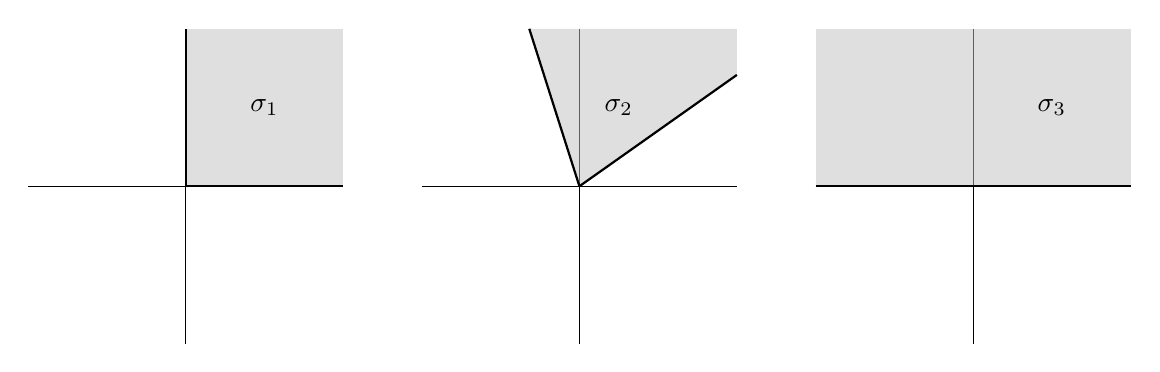
\begin{tikzpicture}
        \begin{scope}[shift={(-5,0)}]
            \draw (-2, 0) -- (2, 0);
            \draw (0, -2) -- (0, 2);
            \fill[fill=gray!50, opacity=0.5] (0, 0) -- (0, 2) -- (2, 2) -- (2, 0);
            \draw[thick] (0, 0) -- (2, 0);
            \draw[thick] (0, 0) -- (0, 2);
            \node at (1, 1) {$\sigma_1$};
        \end{scope}
        \begin{scope}
            \draw (-2, 0) -- (2, 0);
            \draw (0, -2) -- (0, 2);
            \fill[fill=gray!50, opacity=0.5] (0, 0) -- (2, 1.4142135) -- (2, 2) -- (-0.63661977, 2);
            \draw[thick] (0, 0) -- (2, 1.4142135);
            \draw[thick] (0, 0) -- (-0.63661977, 2);
            \node at (0.5, 1) {$\sigma_2$};
        \end{scope}
        \begin{scope}[shift={(5,0)}]
            \draw (-2, 0) -- (2, 0);
            \draw (0, -2) -- (0, 2);
            \fill[fill=gray!50, opacity=0.5] (-2, 0) -- (2, 0) -- (2, 2) -- (-2, 2);
            \draw[thick] (0, 0) -- (2, 0);
            \draw[thick] (0, 0) -- (-2, 0);
            \node at (1, 1) {$\sigma_3$};
        \end{scope}
    \end{tikzpicture} \]
    given by
    \[ \sigma_1 = \RR_{\ge 0} \{ (1, 0), (0, 1) \}, \quad \sigma_2 = \RR_{\ge 0} \{ (\sqrt{2}, 1), (-1, \pi) \}, \quad \sigma_3 = \RR_{\ge 0} \{ (-1, 0), (1, 0) \} .  \]
    Cones $\sigma_1$ and $\sigma_3$ are rational, while $\sigma_2$ is not. Cones $\sigma_1$ and $\sigma_2$ are strongly convex, while $\sigma_3$ is not. All cones have dimension $2$. The faces of $\sigma_1$ are $\{ \{ 0 \}, \RR_{\ge 0} (1, 0), \RR_{\ge 0} (0, 1), \sigma_1 \}$.
\end{example}

\begin{topic}{dual-cone}{dual cone}
    The \textbf{dual cone} of a \tref{polyhedral-cone}{rational polyhedral cone} $\sigma \subset \RR^n$ is
    \[ \sigma^\vee = \{ u \in (\RR^n)^* : \langle u, v \rangle \ge 0 \text{ for all } v \in \sigma \} . \]
\end{topic}

\begin{example}{dual-cone}
    For any polyhedral cone $\sigma \subset \RR^n$, we have $(\sigma^\vee)^\vee = \sigma$. Indeed, it is clear from the definition that $\sigma \subset (\sigma^\vee)^\vee$. Conversely, if $v \not\in \sigma$, then there exists some $u \in \sigma^\vee$ with $\langle u, v \rangle < 0$, so that $v \not\in (\sigma^\vee)^\vee$.
\end{example}

\begin{topic}{fan}{fan}
    A \textbf{fan} in $\RR^n$ is a set $\Delta$ of \tref{polyhedral-cone}{rational strongly convex polyhedral cones}, such that
    \begin{itemize}
        \item every face of a cone in $\Delta$ is also a cone in $\Delta$,
        \item the intersection of two cones in $\Delta$ is a face of each.
    \end{itemize}
\end{topic}

\begin{topic}{gordons-lemma}{Gordon's lemma}
    Let $M$ be a \tref{GT:finitely-generated-group}{finitely generated} \tref{GT:free-group}{free abelian group}, and $\sigma \subset M_\RR = M \otimes_\ZZ \RR$ a \tref{polyhedral-cone}{rational polyhedral cone}. Then \textbf{Gordon's lemma} states that the \tref{AA:monoid}{commutative monoid} $M \cap \sigma$ is finitely generated.
\end{topic}

\begin{example}{gordons-lemma}
    \begin{proof}
        Write $\sigma = \left\{ \sum_{i = 1}^{s} \lambda_i v_i : \lambda_i \in \RR_{\ge 0} \right\}$ for some $v_i \in M$, and let
        \[ K = \left\{ \sum_{i = 1}^{s} t_i v_i : 0 \le t_i \le 1 \right\} \subset M_\RR . \]
        Then $K$ is compact, and since $M$ is discrete, $K \cap M$ is finite. Now take any $u \in M \cap \sigma$, and write $u = \sum_{i = 1}^{s} r_i v_i$ for some $r_i \in \RR_{\ge 0}$. Write $r_i = n_i + t_i$ with $n_i \in \NN$ and $t_i \in [0, 1)$. Then,
        \[ u = \sum_{i = 1}^{s} n_i v_i + \sum_{i = 1}^{s} t_i v_i . \]
        Hence, $M \cap \sigma$ is generated by the $v_i$ and all $K \cap M$.
    \end{proof}
\end{example}

\begin{example}{gordons-lemma}
    Consider $M = \ZZ^2$ and $\sigma = \RR_{\ge 0} \langle (1, 2), (2, 1) \rangle \subset \RR^2$. Gordon's lemma tells us that $M \cap \sigma$ is finitely generated, in particular by the elements $K \cap M = \{ (0, 0), (1, 1), (1, 2), (2, 1), (2, 2), (3, 3) \}$. We can further reduce this to a generating set $\{ (1, 1), (1, 2), (2, 1) \}$.
\end{example}

\begin{topic}{fan-refinement}{fan refinement}
    Let $\Delta$ be a \tref{fan}{fan} in $\RR^n$. A \textbf{refinement} of $\Delta$ is a fan $\Delta'$ in $\RR^n$ such that
    \begin{itemize}
        \item for every $\sigma' \in \Delta'$, there exists some $\sigma \in \Delta$ with $\sigma' \subset \sigma$,
        \item $|\Delta| = |\Delta'|$, where $|\Delta| = \bigcup_{\sigma \in \Delta} \sigma$.
    \end{itemize}
\end{topic}

\begin{example}{fan-refinement}
    The left fan is a refinement of the right fan.
    \[ 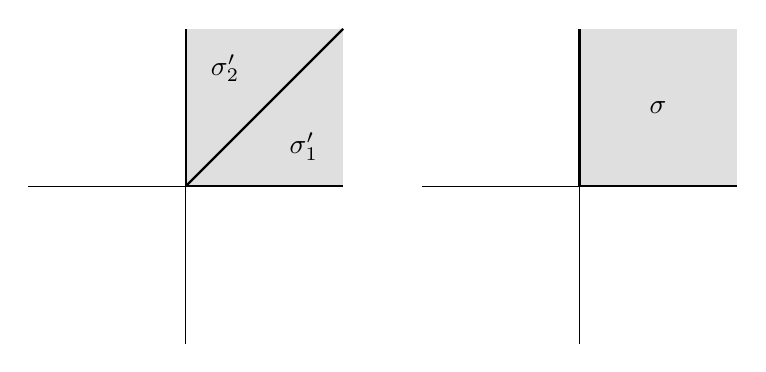
\begin{tikzpicture}
        \begin{scope}[shift={(-5,0)}]
            \draw (-2, 0) -- (2, 0);
            \draw (0, -2) -- (0, 2);
            \fill[fill=gray!50, opacity=0.5] (0, 0) -- (0, 2) -- (2, 2) -- (2, 0);
            \draw[thick] (0, 0) -- (2, 0);
            \draw[thick] (0, 0) -- (0, 2);
            \draw[thick] (0, 0) -- (2, 2);
            \node at (1.5, 0.5) {$\sigma'_1$};
            \node at (0.5, 1.5) {$\sigma'_2$};
        \end{scope}
        \begin{scope}
            \draw (-2, 0) -- (2, 0);
            \draw (0, -2) -- (0, 2);
            \fill[fill=gray!50, opacity=0.5] (0, 0) -- (0, 2) -- (2, 2) -- (2, 0);
            \draw[thick] (0, 0) -- (2, 0);
            \draw[thick] (0, 0) -- (0, 2);
            \node at (1, 1) {$\sigma$};
        \end{scope}
    \end{tikzpicture} \]
\end{example}

\begin{topic}{star-subdivision}{star subdivision}
    Let $\Delta$ be a \tref{fan}{fan} in $\RR^n$, and $\tau \in \Delta$ a cone such that all cones $\sigma \in \Delta$ containing $\tau$ are \textit{smooth}, i.e. $\sigma$ can be generated by a basis of $\RR \cdot \sigma \subset \RR^n$. For any cone $\sigma \in \Delta$, write $\sigma(1)$ for the set of one-dimensional faces of $\sigma$, and for any one-dimensional cone $\rho \in \Delta$, write $u_\rho \in \ZZ^n$ for its minimal generator.
    
    Let $u_\tau = \sum_{\rho \in \tau(1)} u_\rho$, and for each cone $\sigma \in \Delta$ containing $\tau$, let
    \[ \Delta^*_\sigma(\tau) = \left\{ \textup{Cone}(A) \mid A \subset \{ u_\tau \} \cup \{ u_\rho \;:\; \rho \in \sigma(1) \}, \; \{ u_\rho \;:\; \rho \in \tau(1) \} \nsubseteq A \right\} . \]
    The \textbf{star subdivision} of $\Delta$ along $\tau$ is the fan
    \[ \Delta^*(\tau) = \left\{ \sigma \in \Delta \mid \tau \nsubseteq \sigma \right\} \cup \bigcup_{\tau \subset \sigma} \Delta^*_\sigma(\tau) . \]
    % Let $\Delta$ be a \tref{fan}{fan} in $\RR^n$, and $\sigma \in \Delta$ a \textit{smooth cone}, that is, $\sigma = \RR_{\ge 0} \{ v_1, \ldots, v_n \}$ with $v_1, \ldots, v_n \in \ZZ^n$ a basis of $\ZZ^n$. Write $v_0 = v_1 + \cdots + v_n$ and let $\Delta'(\sigma)$ be the set of all cones generated by subsets of $\{ v_0, v_1, \ldots, v_n \}$ not containing $\{ v_1, \ldots, v_n \}$. Then the \textbf{star subdivision} of $\Delta$ along $\sigma$ is the fan
    % \[ \Delta^*(\sigma) = (\Delta \setminus \{ \sigma \}) \cup \Delta'(\sigma) . \]
\end{topic}

\begin{example}{star-subdivision}
    The fan on the left is the star subdivision of the fan on the right along $\tau = \sigma = \RR_{\ge 0} \{ (1, 0), (0, 1) \}$.
    \[ 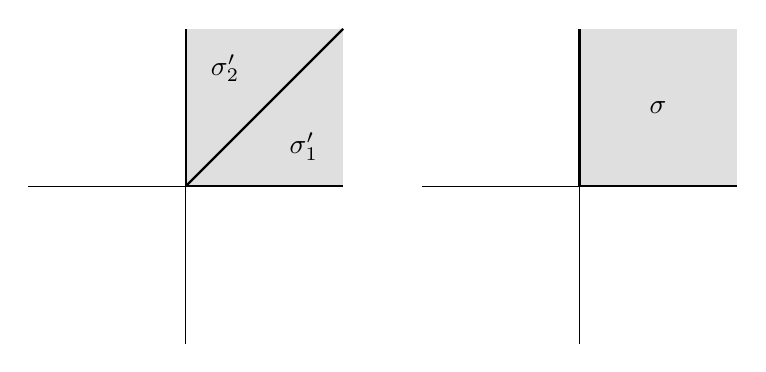
\begin{tikzpicture}
        \begin{scope}[shift={(-5,0)}]
            \draw (-2, 0) -- (2, 0);
            \draw (0, -2) -- (0, 2);
            \fill[fill=gray!50, opacity=0.5] (0, 0) -- (0, 2) -- (2, 2) -- (2, 0);
            \draw[thick] (0, 0) -- (2, 0);
            \draw[thick] (0, 0) -- (0, 2);
            \draw[thick] (0, 0) -- (2, 2);
            \node at (1.5, 0.5) {$\sigma'_1$};
            \node at (0.5, 1.5) {$\sigma'_2$};
        \end{scope}
        \begin{scope}
            \draw (-2, 0) -- (2, 0);
            \draw (0, -2) -- (0, 2);
            \fill[fill=gray!50, opacity=0.5] (0, 0) -- (0, 2) -- (2, 2) -- (2, 0);
            \draw[thick] (0, 0) -- (2, 0);
            \draw[thick] (0, 0) -- (0, 2);
            \node at (1, 1) {$\sigma$};
        \end{scope}
    \end{tikzpicture} \]
\end{example}

\begin{topic}{pick-theorem}{Pick's theorem}
    Let $P$ be a simple polygon in the plane whose vertices have integer coordinates. Let $i$ be the number of lattice points in the interior of $P$, and $b$ the number of lattice points on the boundary of $P$. Then \textbf{Pick's theorem} states that the area $A$ of $P$ is given by
    \[ A = i + \frac{b}{2} - 1 . \]
\end{topic}

\begin{example}{pick-theorem}
    Consider the triangle $\Delta$ with vertices $(0, 0)$, $(x, 0)$ and $(0, y)$. Clearly $A = \frac{1}{2} x y$, and it is not too hard to see that $b = x + y + \gcd(x, y)$. Therefore, the number of interior points of the triangle is
    \[ i = 1 + \frac{1}{2}(xy - x - y - \gcd(x, y)) . \]
\end{example}

\begin{topic}{minkowski-theorem}{Minkowski's theorem}
    Let $L$ be a lattice in $\RR^n$, and $S \subset \RR^n$ a convex subset, which is symmetric with respect to the origin. That is, for all $x \in S$ also $-x \in S$. Then \textbf{Minkowski's theorem} states that if the volume of $S$ is strictly larger than $2^n \det(L)$, then $S$ must contain at least one non-zero lattice point of $L$.
\end{topic}

\begin{example}{minkowski-theorem}
    The given bound is sharp. Namely, consider $L = \ZZ^n$ with $\det(L) = 1$, and $S$ the interior of $[-1, 1]^n$, whose volume is $2^n$. Then $S$ does not contain any non-zero lattice points.
\end{example}

\begin{example}{minkowski-theorem}
    \begin{proof}
        By assumption, the set $\tfrac{1}{2} S = \{ \tfrac{1}{2} x : x \in S \}$ has volume $\textup{vol}(\tfrac{1}{2} S) = 2^{-n} \textup{vol}(S) > \textup{vol}(\RR^n/L)$, so the map $\tfrac{1}{2} S \to \RR^n / L$ cannot be injective. Hence, there are distinct points $x_1, x_2 \in S$ such that $\tfrac{1}{2} x_1 - \tfrac{1}{2} x_2 \in L$. Since $-x_2 \in S$ and $S$ is convex, the linear combination $\tfrac{1}{2} x_1 - \tfrac{1}{2} x_2$ is a non-zero lattice point in $S$.
    \end{proof}
\end{example}

\begin{topic}{root-system}{root system}
    Let $V$ be a finite-dimensional real or complex \tref{vector-space}{vector space} with an \tref{FA:inner-product}{inner product} $(\cdot, \cdot)$. A \textbf{root system} $\Phi$ in $V$ is a finite set of non-zero vectors in $V$, called \textbf{roots}, such that
    \begin{itemize}
        \item (\textit{span}) $\Phi$ spans $V$,
        \item (\textit{multiples}) if $\alpha \in \Phi$, then $n \alpha \in \Phi \iff n = \pm 1$,
        \item (\textit{reflection}) $\beta - \frac{2 (\alpha, \beta)}{(\alpha, \alpha)} \alpha \in \Phi$ for all $\alpha, \beta \in \Phi$,
        \item (\textit{integrality}) $\frac{2 (\alpha, \beta)}{\alpha, \alpha}$ is an integer for all $\alpha, \beta \in \Phi$.
    \end{itemize}
\end{topic}

\begin{example}{root-system}
    Given a complex \tref{AA:semisimple-lie-algebra}{semisimple Lie algebra} $\mathfrak{g}$ and a \tref{AA:cartan-subalgebra}{Cartan subalgebra} $\mathfrak{h} \subset \mathfrak{g}$, one can construct a root system $\Phi$ in $\mathfrak{h}^*$, where a root is an element $\alpha \in \mathfrak{h}^*$ such that
    \[ \mathfrak{g}_\alpha = \{ x \in \mathfrak{g} : [h, x] = \alpha(h) x \textup{ for all } h \in \mathfrak{h} \} \]
    is non-empty.
\end{example}

\begin{topic}{hodge-structure}{Hodge structure}
    Let $R$ be $\ZZ, \QQ$ or $\RR$. An \textbf{$R$-Hodge structure} of weight $k \in \ZZ$ is a pair $H = (H_R, \{ H^{p, q} \})$ consisting of an \tref{AA:module}{$R$-module} $H_R$ of finite rank and a direct sum decomposition of the complexification $H_\CC = H_R \otimes_R \CC$,
    \[ H_\CC = \bigoplus_{p + q = k} H^{p, q} \]
    such that $H^{q, p} = \overline{H^{p, q}}$.

    Equivalently, an \textbf{$R$-Hodge structure} of weight $k \in \ZZ$ is a pair $H = (H_R, F^\bdot)$ consisting of an $R$-module $H_R$ of finite rank and a decreasing filtration $F_\bdot$ on $H_\CC$, called the \textit{Hodge filtration},
    \[ H_\CC \supset \cdots \supset F^p \supset F^{p + 1} \supset \cdots \supset 0 \]
    such that $H_\CC = F^p \oplus \overline{F^q}$ for all $p + q = k + 1$.

    The two descriptions are related via
    \[ F^p = \bigoplus_{r \ge p} H^{r, k - r} \quad \textup{ and } \quad H^{p, q} = F^p \cap \overline{F^q} . \]

    A \textbf{morphism of $R$-Hodge structures} $f : H \to H'$ is a morphism $f : H_R \to H'_R$ of $R$-modules whose complexification $f_\CC$ preserves type, that is, $f_\CC\left(H^{p, q}\right) \subset (H')^{p, q}$.
    
    The numbers $h^{p, q}(H) := \dim_\CC H^{p, q}$ are called the \textbf{Hodge numbers} of the Hodge structure.
\end{topic}

\begin{example}{hodge-structure}
    \begin{itemize}
        \item For any $H_R$, taking $H^{k, k} = H_\CC$ and $H^{p, q} = 0$ when $(p, q) \ne (k, k)$ gives the \textit{trivial Hodge structure} of weight $2k$.
        \item Take $H_\ZZ = 2 \pi i \ZZ \subset \CC$ and $H_\CC = H^{-1, -1}$. This is a Hodge structure of weight $-2$. In fact, is the unique $1$-dimensional Hodge structure of weight $-2$ up to isomorphism, and it is called the \textit{Tate Hodge structure}, often denoted by $\ZZ(1)$.
    \end{itemize}
\end{example}

\begin{example}{hodge-structure}
    Let $M$ be a \tref{TO:compact-space}{compact} \tref{DG:kahler-manifold}{Kähler manifold} of dimension $2n$. The \textit{Hodge decomposition theorem} states that the \tref{DG:de-rham-cohomology}{de Rham cohomology} of $M$ carries an $\RR$-Hodge structure
    \[ H_\textup{dR}^k(M) \otimes_\RR \CC \cong \bigoplus_{p + q = k} H^{p, q}(M) , \]
    where $H^{p, q}(M)$ are the cohomology classes whose \textit{harmonic representative} is of type $(p, q)$.
\end{example}

\begin{topic}{hodge-polynomial}{Hodge polynomial}
    The \textbf{Hodge polynomial} of a \tref{hodge-structure}{Hodge structure} $H$ is the polynomial,
    \[ P_\textup{hodge}(H) = \sum_{p, q \in \ZZ} h^{p, q}(H) u^p v^q , \]
    where $h^{p, q}(H) = \dim_\CC H^{p, q}$ denote the Hodge numbers.
\end{topic}

\begin{topic}{mixed-hodge-structure}{mixed Hodge structure}
    Let $R$ be $\ZZ, \QQ$ or $\RR$. An \textbf{$R$-mixed Hodge structure} is a triple $H = (H_R, W_\bdot, F^\bdot)$ consisting of an $R$-module $H_R$, an increasing filtration $W_\bdot$ on $H_{R \otimes \QQ} = H_R \otimes \QQ$,
    \[ 0 \subset \cdots \subset W_k \subset W_{k + 1} \cdots \subset H_\QQ \]
    and a decreasing filtration $F^\bdot$ on $H_\CC = H_R \otimes \CC$,
    \[ H_\CC \supset \cdots \supset F^p \supset F^{p + 1} \supset \cdots \supset 0 \]
    such that the induced filtrations (obtained by intersections) of $F^\bdot$ on the graded pieces $\left(\textup{Gr}^W_k H_\QQ\right) \otimes_\QQ \CC := \left(W_k H_\QQ / W_{k - 1} H_\QQ\right) \otimes \CC$ are \tref{hodge-structure}{rational Hodge structures} of weight $k$.
    
    A \textbf{morphism of $R$-mixed Hodge structures} is a morphism $f : H_R \to H'_R$ of $R$-modules compatible with the two filtrations $W_\bdot$ and $F^\bdot$.
    
    The numbers $h^{p, q}(H) \coloneqq \dim_\CC \textup{Gr}_F^p \textup{Gr}^W_{p + q}(H_\CC)$ are called the \textbf{mixed Hodge numbers} of the mixed Hodge structure $H$.
\end{topic}

\begin{topic}{polarized-hodge-structure}{polarized Hodge structure}
    Let $R$ be $\ZZ$, $\QQ$ or $\RR$. A \textbf{polarization} of an \tref{hodge-structure}{$R$-Hodge structure} $(H_R, F^\bdot)$ of weight $k$ is an $R$-valued bilinear form
    \[ Q : H_R \otimes_R H_R \to R \]
    such that
    \begin{itemize}
        \item $Q(v, w) = (-1)^k Q(w, v)$ for all $v, w \in H_R$,
        \item the orthogonal complement of $F^m$ is $F^{k - m + 1}$ for all $m \in \ZZ$,
        \item the Hermitian form on $H_\CC = H_R \otimes \CC$ given by $v \otimes w \mapsto Q(C u, \overline{v})$, where $C$ is the \textit{Weil operator} $C|_{H^{p, q}} = i^{p - q}$, is \tref{LA:definite-matrix}{positive-definite}.
    \end{itemize}
\end{topic}

\begin{topic}{inner-product}{inner product}
    An \textbf{inner product} on a \tref{LA:vector-space}{vector space} $V$ over $k = \RR$ or $\CC$ is a map $\langle \cdot, \cdot \rangle : V \times V \to k$ satisfying
    \begin{itemize}
        \item (\textit{linearity}) $\langle \alpha x + \beta y, z \rangle = \alpha \langle x, z \rangle + \beta \langle y, z \rangle$ for all scalars $\alpha$ and $x, y, z \in V$,
        \item \textit{(conjugate symmetry)} $\langle x, y \rangle = \overline{\langle y, x \rangle}$ for all $x, y \in V$,
        \item (\textit{positive definiteness}) $\langle x, x \rangle > 0$ for all $x \ne 0$ in $V$.
    \end{itemize}
    A vector space together with an inner product is called an \textbf{inner product space}.
\end{topic}

\begin{topic}{cauchy-schwarz-inequality}{Cauchy--Schwarz inequality}
    The \textbf{Cauchy--Schwarz inequality} states that for any vectors $v, w$ in an \tref{inner-product}{inner-product-space},
    \[ \langle v, w \rangle^2 \le \langle v, v \rangle \cdot \langle w, w \rangle . \]
\end{topic}

\begin{topic}{polarization-identity}{polarization identity}
    Let $(V, \langle \cdot, \cdot \rangle)$ be an \tref{inner-product}{inner product space}. The polarization identity states that
    \[ \operatorname{Re} \langle x, y \rangle = \frac{1}{2} ( \norm{x + y} - \norm{x} - \norm{y} ) , \]
    where $\norm{x} = \langle x, x \rangle$.
\end{topic}


\chapter{Group Theory}
\renewcommand{\cat}{GT}
\begin{topic}{group}{group}
    A \textbf{group} is a set $G$ together with an operation $G \times G \to G$ (the \textit{group law}) written as $(x, y) \mapsto xy$, and an element $1 \in G$ (the \textit{unit}), satisfying
    \begin{itemize}
        \item (\textit{associativity}) $(xy)z = x(yz)$ for all $x, y, z \in G$,
        \item (\textit{unit element}) $1 \cdot x = x \cdot 1 = x$ for all $x \in G$,
        \item (\textit{inverses}) for all $x \in G$ there exists an $x^{-1} \in G$ such that $x x^{-1} = x^{-1} x = 1$, called the \textit{inverse} of $x$.
    \end{itemize}
\end{topic}

\begin{topic}{subgroup}{subgroup}
    A \textbf{subgroup} $H$ of a \tref{group}{group} $G$ is a subset $H \subset G$ which, with the same group law and unit, is itself a group.
\end{topic}

\begin{topic}{abelian-group}{abelian group}
    A \tref{group}{group} $G$ is called \textbf{abelian} if $xy = yx$ for all $x, y \in G$.
\end{topic}

\begin{topic}{order}{order}
    Let $G$ be a \tref{group}{group}. The \textbf{order} of an element $x \in G$, denoted $\text{ord}(x)$, is the least positive integer $n$ such that $x^n = 1$. If no such $n$ exists, then $\text{ord}(x) = \infty$.
\end{topic}

\begin{topic}{cyclic-group}{cyclic group}
    A \textbf{cyclic group} is a \tref{group}{group} $G$ generated by a single element $x \in G$, that is $G = \{ x^n : x \in \ZZ \}$.
\end{topic}

\begin{topic}{group-homomorphism}{group homomorphism}
    Let $G$ and $H$ be two \tref{group}{groups}. A \textbf{homomorphism} from $G$ to $H$ is a map $f : G \to H$ satisfying $f(xy) = f(x) f(y)$ for all $x, y \in G$.
\end{topic}

\begin{topic}{kernel}{kernel}
    Let $f : G \to H$ be a \tref{group-homomorphism}{group homomorphism}. The \textbf{kernel} of $f$, denoted $\ker f$, is defined as
    \[ \ker f = \{ x \in G : f(x) = 0 \} . \]
    It is a \tref{normal-subgroup}{normal} \tref{subgroup}{subgroup} of $G$.
\end{topic}

\begin{topic}{group-center}{group center}
    The \textbf{center} of a \tref{group}{group} $G$ is the subgroup
    \[ Z(G) = \{ x \in G : xy = yx \text{ for all } y \in G \} . \]
\end{topic}

\begin{topic}{symmetric-group}{symmetric group}
    Let $\Sigma$ be a set. The \textbf{symmetric group} on $\Sigma$ is the \tref{group}{group} $S_\Sigma$ of all bijections $\Sigma \to \Sigma$. The group law is given by composition, and the unit is the identity map.
    
    When $\Sigma = \{ 1, 2, \ldots, n \}$ for some integer $n \ge 1$, one writes $S_n$ for the symmetry group. Its elements are called \textbf{permutations}.
\end{topic}

\begin{topic}{cayleys-theorem}{Cayley's theorem}
    \textbf{Cayley's theorem} states that every \tref{group}{group} $G$ is isomorphic to a \tref{subgroup}{subgroup} of the \tref{symmetric-group}{symmetric group} $S_G$. In particular, $G$ is isomorphic to the image of the morphism
    \[ \varphi : G \to S_G, \qquad x \mapsto (y \mapsto xy) . \]
\end{topic}

\begin{topic}{cyclic-permutation}{cyclic permutation}
    A \tref{symmetric-group}{permutation} $\sigma \in S_n$ is a \textbf{cyclic permutation}, or \textbf{cycle}, of length $k$ if there exist $k$ distinct integers $1 \le a_1, \ldots, a_k \le n$ with $\sigma(a_i) = a_{i + 1}$ for $1 \le i < k$ and $\sigma(a_k) = a_1$, and $\sigma(x) = x$ for $x \not\in \{ a_1, \ldots, a_k \}$. This is denoted by
    \[ \sigma = (a_1 \;\; a_2 \;\; \ldots \;\; a_k) . \]
    A cycle of length $2$ is also called a \textbf{transposition}.
\end{topic}

\begin{topic}{permutation-sign}{permutation sign}
    The \textbf{sign} of a \tref{symmetric-group}{permutation} $\sigma \in S_n$ is defined as
    \[ \text{sign}(\sigma) = \prod_{1 \le i < j \le n} \frac{\sigma(j) - \sigma(i)}{j - i} \in \{ +1, -1 \} . \]
    We call $\sigma$ \textit{even} if $\text{sign}(\sigma) = 1$ and \textit{odd} if $\text{sign}(\sigma) = -1$.
    
    This defines a \tref{group-homomorphism}{group homomorphism}
    \[ \text{sign} : S_n \to \{ +1, -1 \} . \]
\end{topic}

\begin{topic}{alternating-group}{alternating group}
    For $n \ge 1$, the \textbf{alternating group} $A_n$ is the subgroup of the \tref{symmetric-group}{symmetric group} $S_n$ of all \tref{permutation-sign}{even} permutations.
\end{topic}

\begin{topic}{normal-subgroup}{normal subgroup}
    A \tref{subgroup}{subgroup} $N$ of a \tref{group}{group} $G$ is called \textbf{normal} if $N = g N g^{-1}$ for all $g \in G$.
\end{topic}

\begin{example}{normal-subgroup}
    The \tref{kernel}{kernel} of a morphism $f : G \to H$ is always a normal subgroup. Indeed, for any $x \in \ker f$ and $g \in G$ we have
    \[ f(gxg^{-1}) = f(g) f(x) f(g)^{-1} = f(g) f(g)^{-1} = 1 , \]
    so $gxg^{-1} \in \ker f$, and thus $g (\ker f) g^{-1} \subset \ker f$. The other inclusion is shown completely similarly.
    
    Conversely, any normal subgroup $N \subset G$ is the kernel of the quotient map $\pi : G \to G / N$.
\end{example}

\begin{topic}{central-subgroup}{central subgroup}
    A \tref{subgroup}{subgroup} $H$ of a \tref{group}{group} $G$ is called \textbf{central} if $H$ lies in the \tref{group-center}{center} of $G$.
\end{topic}

\begin{topic}{quotient-group}{quotient group}
    Let $G$ be a \tref{group}{group} and $N$ a \tref{normal-subgroup}{normal subgroup}. The \textbf{quotient group} $G/N$ is the group of cosets
    \[ G/N = \{ gN : g \in G \} \]
    with group law $(gN)(hN) = (gh)N$ and unit $N$.
\end{topic}

\begin{topic}{simple-group}{simple group}
    A \tref{group}{group} $G$ is called \textbf{simple} if its only \tref{normal-subgroup}{normal subgroups} are $\{ 1 \}$ and $G$.
\end{topic}

\begin{topic}{torsion-subgroup}{torsion subgroup}
    The \textbf{torsion subgroup} of a \tref{group}{group} $G$ is the subgroup of elements of finite \tref{order}{order}.
    \[ G_{\text{tor}} = \{ x \in G : \text{ord}(x) < \infty \} \]
\end{topic}

\begin{topic}{normalizer}{normalizer}
    Let $H$ be a \tref{subgroup}{subgroup} of a \tref{group}{group} $G$. The \textbf{normalizer} of $H$ is the subgroup
    \[ N_H = \{ x \in G : x H x^{-1} = H \} . \]
\end{topic}

\begin{topic}{group-action}{group action}
    Let $G$ be a \tref{group}{group} and $X$ a set. An \textbf{action} of $G$ on $X$ is map
    \[ G \times X \to X : (g, x) \mapsto g \cdot x \]
    satisfying $1 \cdot x = x$ and $g \cdot (h \cdot x) = (gh) \cdot x$ for all $g, h \in G$ and $x \in X$.
\end{topic}

\begin{topic}{centralizer}{centralizer}
    Let $G$ be a \tref{group}{group}. The \textbf{centralizer} of an element $g \in G$ is the subgroup
    \[ G_g = \{ h \in G : h x h^{-1} = g \} . \]
\end{topic}

\begin{topic}{stabilizer}{stabilizer}
    Let $G$ be a \tref{group}{group} \tref{group-action}{acting} on a set $X$. Then the \textbf{stabilizer} of $x \in X$ is the \tref{subgroup}{subgroup}
    \[ G_x = \{ g \in G : g \cdot x = x \} . \]
\end{topic}

\begin{topic}{orbit}{orbit}
    Let $G$ be a \tref{group}{group} \tref{group-action}{acting} on a set $X$. The \textbf{orbit} of an element $x \in X$ is the set
    \[ Gx = \{ g \cdot x : g \in G \} \subset X . \]
\end{topic}

\begin{topic}{solvable-group}{solvable group}
    A \tref{group}{group} $G$ is \textbf{solvable} if there exist \tref{subgroup}{subgroups} $H_1, H_2, \ldots, H_r$
    \[ G = H_0 \supset H_1 \supset \cdots \supset H_r = \{ 1 \} \]
    where $H_{i + 1}$ is \tref{normal-subgroup}{normal} in $H_i$ and $H_i/H_{i + 1}$ is abelian.
\end{topic}

\begin{example}{solvable-group}
    The group $S_3$ is solvable, since we have the sequence $S_3 \supset A_3 \supset \{ 1 \}$, and $S_3 / A_3 \simeq \ZZ/2\ZZ$ and $A_3/\{ 1 \} \simeq \ZZ/3\ZZ$.
\end{example}

\begin{topic}{commutator-subgroup}{commutator subgroup}
    The \textbf{commutator subgroup} of a \tref{group}{group} $G$ is the subgroup of $G$ generated by all elements of the form $ghg^{-1}h^{-1}$ with $g, h \in G$.
\end{topic}

\begin{topic}{conjugation}{conjugation}
    Let $G$ be a \tref{group}{group}. Two elements $x, y \in G$ are called \textbf{conjugate} if there exists some $g \in G$ such that $g x g^{-1} = y$.
\end{topic}

\begin{topic}{free-group}{free (abelian) group}
    Given a set $S$, the \textbf{free group} over $S$, denoted $F_S$, is the \tref{group}{group} consisting of all words that can be built from elements of $S$ and $\{ s^{-1} : s \in S \}$, where two words are different unless their equality follows from the group axioms. Composition is given by concatenation of words, and the unit element is the empty word. The members of $S$ are called \textit{generators} of $F_S$, and the number of generators (i.e. the size of $S$) is the \textit{rank} of $F_S$.

    The \textbf{free abelian group} over $S$ is the \tref{abelian-group}{abelian} group $\bigoplus_{s \in S} \ZZ$.
\end{topic}

% // Borel subgroup
% Dihedral group
% Subgroup index
% Lagrange's theorem
% Sylow p-group



\chapter{Representation Theory}
\renewcommand{\cat}{RT}
\begin{topic}{representation}{representation}
    A \textbf{representation} of a \tref{GT:group}{group} $G$ on a \tref{LA:vector-space}{vector space} $V$ over a \tref{AA:field}{field} $k$ is a \tref{GT:group-homomorphism}{group homomorphism}
    \[ \rho : G \to \textup{GL}(V) . \]
    The vector space $V$ is called the \textit{representation space} and $\dim_k V$ the \textit{dimension} of the representation.
\end{topic}

\begin{topic}{irreducible-representation}{(ir)reducible representation}
    A \tref{representation}{representation} $\rho : G \to \textup{GL}(V)$ is \textbf{reducible} if there exists a non-zero proper invariant subspace $W \subset V$, that is, $\rho(g) w \in W$ for all $w \in W$ and $g \in G$. If no such subspace exists, the representation is \textbf{irreducible}. % If $\rho$ can be written as a direct sum $\rho_1 \oplus \rho_2$, then it is called \textbf{reducible}.
\end{topic}

\begin{topic}{faithful-representation}{faithful representation}
    A \tref{representation}{representation} $\rho : G \to \textup{GL}(V)$ is \textbf{faithful} if $\rho$ is injective.
\end{topic}

\begin{topic}{unitary-representation}{unitary representation}
    A \tref{representation}{representation} $\rho : G \to \textup{GL}(V)$ over $\CC$ is \textbf{unitary} if $\rho(g)$ is unitary for all $g \in G$, that is $\rho(g)^\dagger \rho(g) = \rho(g) \rho(g)^\dagger = \id_V$.
\end{topic}

\begin{topic}{character}{character}
    The \textbf{character} of a \tref{representation}{representation} $\rho : G \to \textup{GL}(V)$ is the function
    \[ \chi_\rho : G \to k, \quad g \mapsto \textup{tr}(\rho(g)) . \]
    Note that $\chi_\rho$ is constant on conjugacy classes.
\end{topic}

\begin{topic}{representation-ring}{representation ring}
    Given a \tref{GT:group}{group} $G$ and a \tref{AA:field}{field} $k$, the \textbf{representation ring} $R_k(G)$ is the \tref{GT:free-group}{free abelian group} on isomorphism classes of finite-dimensional \tref{representation}{$k$-representations} of $G$. For the ring structure, addition is given by the direct sum of representations, and multiplication by their tensor product over $k$.
    
    Equivalently, the representation ring $R_k(G)$ is the \tref{HA:grothendieck-group}{Grothendieck ring} of the category of finite-dimensional representations of $G$.
\end{topic}

\begin{example}{representation-ring}
    \begin{itemize}
        \item Any representation of $G = \textup{GL}_1(\CC) = \CC^*$ is a direct sum of $1$-dimensional representations of the form $\rho_n : \CC^* \to \CC^*, z \mapsto z^n$ for some character $n \in \ZZ$. Hence the representation ring of $G$ is $R_\CC(G) = \ZZ[t, t^{-1}]$, where $t$ corresponds to $\rho_1$.
        
        \item Any representation of the cyclic group $G = \ZZ/n\ZZ$ is a direct sum of $1$-dimensional representations which sends $1 \textup{ mod } n$ to an $n$-th root of unity. Hence the (complex) representation ring of $G$ is $R_\CC(G) = \ZZ[t]/(t^n - 1)$, where $t$ corresponds to the representation $1 \mapsto \zeta_n$, a primitive root of unity.
    \end{itemize}
\end{example}

\begin{topic}{equivalent-representations}{equivalent representations}
    Two \tref{representation}{representations} $\rho : G \to \textup{GL}(V)$ and $\rho' : G \to \textup{GL}(W)$ are called \textbf{equivalent}, or \textbf{isomorphic}, if there exists a linear isomorphism $A : V \to W$ such that $\rho'(g) = A \rho(g) A^{-1}$ for all $g \in G$.
\end{topic}

\begin{topic}{schur-lemma}{Schur's lemma}
    Let $G$ be a \tref{GT:group}{group}. \textbf{Schur's lemma} states:
    \begin{enumerate}[(i)]
        \item If $\rho : G \to \textup{GL}(V)$ and $\rho' : G \to \textup{GL}(W)$ are two \tref{equivalent-representations}{inequivalent} \tref{irreducible-representation}{irreducible} \tref{representation}{representations}, and $A : V \to W$ is a linear map such that $A \rho(g) = \rho'(g) A$ for all $g \in G$, then $A = 0$.
        \item If $\rho : G \to \textup{GL}(V)$ is an irreducible representation over an \tref{AA:algebraically-closed-field}{algebraically closed field $k$}, and $A : V \to V$ is a linear map such that $A \rho(g) = \rho(g) A$ for all $g \in G$, then $A$ is a scalar multiple of the identity map.
    \end{enumerate}
\end{topic}

\begin{example}{schur-lemma}
    \begin{proof}
    \begin{enumerate}[(i)]
        \item For any vector $v \in V$ and $g \in G$ we have
        \[ A \rho(g) v = \rho'(g) A v . \]
        This shows that $\im A$ is invariant under $\rho'$, and $\ker A$ is invariant under $\rho$. Since both $\rho$ and $\rho'$ are irreducible, it follows that $\im A$ equal to $0$ or $W$, and $\ker A$ equal to $0$ or $V$. If $A \ne 0$, then we must have $\im A = W$ and $\ker A = 0$, implying that $A$ is invertible. But then $\rho'(g) = A \rho(g) A^{-1}$, contradicting the inequivalence of representations.
        \item Let $v \in V$ be an eigenvector of $A$ with eigenvalue $\lambda \in k$. Then for all $g \in G$,
        \[ A \rho(g) v = \rho(g) A v = \lambda \rho(g) v , \]
        so $\rho(g) v$ is again an eigenvector of $A$ with eigenvalue $\lambda$. This shows that the eigenspace of $A$ corresponding to $\lambda$ is invariant under $\rho$. Since $\rho$ is irreducible, this eigenspace must be $0$ or $V$, and since it contains $v$ already, it must be $V$. We conclude that $A = \lambda I$.
    \end{enumerate}
    \end{proof}
\end{example}

\begin{topic}{clebsch-gordan-series}{Clebsch--Gordan series}
    Let $G$ be a finite \tref{GT:group}{group}, and $\rho_i, \rho_j$ two \tref{irreducible-representation}{irreducible} \tref{representation}{representations} of $G$. The tensor product $\rho_i \otimes \rho_j$ is generally reducible, and can be written as
    \[ \rho_i \otimes \rho_j = A \left( \bigoplus_k a^k_{ij} \rho_k \right) A^{-1} , \]
    for some invertible $A$. The coefficients $a^k_{ij}$ are called the \textbf{Clebsch--Gordan series}. The matrix entries of $A$ in some standard basis are called the \textbf{Clebsch--Gordan coefficients}.
\end{topic}

\begin{topic}{projective-representation}{projective representation}
    A \textbf{projective representation} of a \tref{GT:group}{group} $G$ on a \tref{LA:vector-space}{vector space} $V$ over a field $k$ is a \tref{GT:group-homomorphism}{group homomorphism}
    \[ \rho : G \to \textup{PGL}(V) , \]
    where $\textup{PGL}(V) = \textup{GL}(V) / k^*$ is the \tref{LA:projective-linear-group}{projective linear group} of $V$.
\end{topic}

\begin{example}{projective-representation}
    The universal (double) cover of the \tref{LA:orthogonal-group}{special orthogonal group} $\textup{SO}(3)$ is the \tref{LA:unitary-group}{special unitary group} $\textup{SU}(2)$. Hence, any representation $\rho : \textup{SU}(2) \to \textup{GL}(V)$ descends to a projective representation $\pi : \textup{SO}(3) \to \textup{PGL}(V)$, which can be lifted to an honest representation if and only if the dimension of $V$ is odd. For example, the standard representation $\textup{SU}(2) \to \textup{GL}(\CC^2)$ induces a projective representation
    \[ \textup{SO}(3) \to \textup{PGL}(\CC^2) \]
    which cannot be lifted to an honest representation.
\end{example}

% \begin{example}{projective-representation}
%     Any representation $\rho : G \to \textup{GL}(V)$ can be composed with $\textup{GL}(V) \to \textup{PGL}(V)$ to give a projective representation, but the converse is not true. Consider $G = \textup{SO}(3)$ and $\rho : G \to \textup{PGL}_2(\CC)$ induced by
%     \[ \mathfrak{so}(3) \to \textup{GL}_2(\CC), \quad \sigma_1 \mapsto \begin{pmatrix}  \end{pmatrix}, \quad \sigma_2 \mapsto \begin{pmatrix} \end{pmatrix}, \quad \sigma_3 \mapsto \begin{pmatrix} \end{pmatrix} . \]
% \end{example}

\begin{topic}{dual-representation}{dual representation}
    The \textbf{dual representation} of a \tref{representation}{representation} $\rho : G \to \textup{GL}(V)$ is the representation on the \tref{LA:dual-vector-space}{dual vector space} $V^*$ given by
    \[ \rho^* : G \to \textup{GL}(V^*), \quad g \mapsto \rho(g^{-1})^T = (-) \circ \rho(g^{-1}) . \]
\end{topic}

\begin{topic}{first-orthogonality-theorem}{first orthogonality theorem}
    Let $G$ be a finite \tref{GT:group}{group} and let $\rho_1 : G \to \textup{GL}(V)$ and $\rho_2 : G \to \textup{GL}(W)$ be two \tref{irreducible-representation}{irreducible representations} over $\CC$ with corresponding \tref{character}{characters} $\chi_1$ and $\chi_2$. Then the \textbf{first orthogonality theorem} states that
    \[ \frac{1}{|G|} \sum_{g \in G} \chi_1(g) \overline{\chi_2(g)} = \left\{ \begin{array}{cl} 1 & \textup{ if } \rho_1 \simeq \rho_2 , \\ 0 & \textup{ if } \rho_1 \not\simeq \rho_2 , \end{array} \right. \]
    where $\simeq$ denotes \tref{equivalent-representations}{equivalence}.
\end{topic}

\begin{example}{first-orthogonality-theorem}
    \begin{proof}
        Let $A : W \to V$ be an arbitrary linear map, and take
        \[ B = \sum_{g \in G} \rho_1(g) A \rho_2(g^{-1}) . \]
        Note that
        \[ \rho_1(h) B = \sum_{g \in G} \rho_1(hg) A \rho_2(g^{-1}) = \sum_{g' \in G} \rho_1(g') A \rho_2(g'^{-1} h) = B \rho_2(h) . \]
        If $\rho_1 \simeq \rho_2$, then \tref{schur-lemma}{Schur's first lemma} implies $B = \lambda I$ for some $\lambda \in \CC$, and if $\rho_1 \not\simeq \rho_2$, then \tref{schur-lemma}{Schur's second lemma} yields $B = 0$. Now taking $A_{\ell m} = \delta_{\ell r} \delta_{ms}$, in terms of some basis for $V$ and $W$, gives
        \[ \sum_{g \in G} (\rho_1(g))_{ir} (\rho_2(g^{-1}))_{sj} = \left\{ \begin{array}{cl} \lambda_{rs} \delta_{ij} & \textup{ if } \rho_1 \simeq \rho_2 , \\ 0 & \textup{ if } \rho_1 \not\simeq \rho_2 . \end{array} \right. \]
        Whenever $\rho_1 \simeq \rho_2$, we can set $i = j$ and sum over $i$ to obtain $|G| \delta_{rs} = \lambda_{rs} \dim_\CC(V)$. Substituting this into the above, setting $r = i$ and $s = j$ and summing over $i$ and $j$ now gives
        \[ \sum_{g \in G} \chi_1(g) \chi_2(g^{-1}) = \left\{ \begin{array}{cl} |G| & \textup{ if } \rho_1 \simeq \rho_2 , \\ 0 & \textup{ if } \rho_1 \not\simeq \rho_2 , \end{array} \right. \]
        as desired.
    \end{proof}
\end{example}

\begin{example}{first-orthogonality-theorem}
    Define an inner product on the characters of $G$,
    \[ \langle \chi_1, \chi_2 \rangle = \frac{1}{|G|} \sum_{g \in G} \chi_1(g) \chi_2(g^{-1}) . \]
    The first orthogonality theorem now says that $\langle \chi, \chi \rangle = 1$ for any character $\chi$, and that inequivalent characters are orthogonal. In particular, two irreducible representations $\rho_1$ and $\rho_2$ are equivalent if and only if their characters are equal. Namely, if $\rho_1 \not\simeq \rho_2$, then $\langle \chi_1, \chi_2 \rangle = 0$, and since $\langle \chi_1, \chi_1 \rangle = 1$, we must have $\chi_1 \ne \chi_2$.
\end{example}


\chapter{Topology}
\renewcommand{\cat}{TO}
\begin{topic}{topological-space}{topological space}
    A \textbf{topological space} is a set $X$ together with family $\mathcal{T}$ of subsets of $X$ satisfying
    \begin{itemize}
        \item $X, \varnothing \in \mathcal{T}$,
        \item the intersection of any two sets in $\mathcal{T}$ is in $\mathcal{T}$,
        \item the union of any collection of sets in $\mathcal{T}$ is in $\mathcal{T}$.
    \end{itemize}
    The family $\mathcal{T}$ is called a \textbf{topology} for $X$, and the members of $\mathcal{T}$ are referred to as \textbf{open sets}. A subset $V \subset X$ is called \textbf{closed} if its complement $X \backslash V$ is open.
\end{topic}

\begin{topic}{discrete-topology}{discrete topology}
    Let $X$ be a set. The \textbf{discrete topology} on $X$ is the topology where all subsets of $X$ are open.
\end{topic}

\begin{topic}{indiscrete-topology}{indiscrete topology}
    Let $X$ be a set. The \textbf{indiscrete topology} on $X$ is the topology where only $\varnothing$ and $X$ are open.
\end{topic}

\begin{topic}{coarser}{coarser/finer topology}
    Given two \tref{topological-space}{topologies} $\mathcal{T}_1$ and $\mathcal{T}_2$ on the same set. Then $\mathcal{T}_1$ is called \textbf{coarser} than $\mathcal{T}_2$ if $\mathcal{T}_1 \subset \mathcal{T}_2$. Equivalently, $\mathcal{T}_2$ is called \textbf{finer} than $\mathcal{T}_1$.
\end{topic}

\begin{topic}{continuous-map}{continuous map}
    A map $f : X \to Y$ between \tref{topological-space}{topological spaces} is \textbf{continuous} if for every open subset $V \subset Y$, the inverse image $f^{-1}(V)$ is open in $X$.
\end{topic}

\begin{topic}{homeomorphism}{homeomorphism}
    A map $f : X \to Y$ between \tref{topological-space}{topological spaces} is a \textbf{homeomorphism} if it is \tref{continuous-map}{continuous}, bijective and its inverse is continuous as well.
\end{topic}

\begin{topic}{closure}{closure}
    Let $X$ be a \tref{topological-space}{topological space}, and $A \subset X$ a subset. A point $x \in X$ is a \textbf{point of closure} of $A$ if $U \cap A \ne \varnothing$ for any open subset $U \subset X$ with $x \in U$. The \textbf{closure} $\overline{A}$ of $A$ is the set of points of closure of $A$.
    
    Equivalently, $\overline{A}$ is the smallest closed subset of $X$ containing $A$.
    % In particular, $\overline{A}$ is closed, $A \subset \overline{A}$ and $\overline{\overline{A}} = \overline{A}$.
\end{topic}

\begin{topic}{interior}{interior}
    Let $X$ be a \tref{topological-space}{topological space}, and $A \subset X$ a subset. A point $x \in X$ is an \textbf{interior point} of $A$ if there exists an open set $U \subset A$ with $x \in U$. The \textbf{interior} $\overset{\circ}{A}$ of $A$ is the set of interior points of $A$.
    
    Equivalently, $\overset{\circ}{A}$ is the largest open subset of $X$ contained in $A$.
\end{topic}

\begin{topic}{boundary}{boundary}
    The \textbf{boundary} $\partial A$ of a subset $A$ of a \tref{topological-space}{topological space} $X$ is the set $\overline{A} \backslash \overset{\circ}{A}$.
\end{topic}

\begin{topic}{neighborhood}{neighborhood}
    A \textbf{neighborhood} of a point $x$ in a \tref{topological-space}{topological space} $X$ is a subset $V \subset X$ that includes an open set $U \subset X$ containing $x$.
    \[ x \in U \subset V \]
\end{topic}

\begin{topic}{basis}{basis}
    Given a \tref{topological-space}{topological space} $X$ with topology $\mathcal{T}$, a \textbf{basis} for $\mathcal{T}$ is a subfamily $\mathcal{B} \subset \mathcal{T}$ such that every set in $\mathcal{T}$ is a union of sets from $\mathcal{B}$.
\end{topic}

\begin{topic}{subbasis}{subbasis}
    Given a \tref{topological-space}{topological space} $X$ with topology $\mathcal{T}$, a \textbf{subbasis} for $\mathcal{T}$ is a subfamily $\mathcal{B} \subset \mathcal{T}$ such that $\mathcal{B}$ \textit{generates} $\mathcal{T}$. That is, every open set in $\mathcal{T}$ is a union of finite intersections of sets of $\mathcal{B}$.
\end{topic}

\begin{topic}{second-countable}{second countable}
    A \tref{topological-space}{topological space} which admits a countable \tref{basis}{basis} is called \textbf{second countable}.
\end{topic}

\begin{topic}{dense}{dense}
    A subset $A$ of a \tref{topological-space}{topological space} $X$ is \textbf{dense} if its \tref{closure}{closure} $\overline{A}$ equals $X$.
\end{topic}

\begin{topic}{quasi-compact}{quasi-compact}
    A \tref{topological-space}{topological space} $X$ is \textbf{quasi-compact} if every open covering of $X$ has a finite subcover.
    
    A continuous map $f : X \to Y$ is \textbf{quasi-compact} if the inverse image $f^{-1}(V)$ of every quasi-compact open $V \subset Y$ is quasi-compact.
\end{topic}

\begin{topic}{specialization}{specialization}
    Let $X$ be a \tref{topological-space}{topological space}. If $x, y \in X$ then we say $y$ is a \textbf{specialization} of $x$, (sometimes that $x$ is a \textbf{generalization} of $y$) if $y \in \overline{\{ x \}}$, i.e. $y$ lies in the \tref{closure}{closure} of $x$. This is denoted as $x \leadsto y$.
    
    A subset $T \subset X$ is said to be \textbf{stable under specialization} if for all $x \in T$ and every specialization $x \leadsto y$ we have $y \in T$.
    
    Similarly, a subset $T \subset X$ is said to be \textbf{stable under generalization} if for all $y \in T$ and every generalization $x \leadsto y$ we have $x \in T$.
\end{topic}

\begin{topic}{closed-map}{closed map}
    A \tref{continuous-map}{continuous map} $f : X \to Y$ is a \textbf{closed map} if for all closed subsets $Z \subset X$, the image $f(Z)$ is closed in $Y$.
\end{topic}

\begin{topic}{universally-closed}{universally closed}
    A continuous map $f : X \to Y$ is \textbf{universally closed} if for all $g : Z \to Y$ the pullback $X \times_Y Z \to Z$ is \tref{closed-map}{closed}.
\end{topic}

\begin{topic}{irreducible}{irreducible}
    A \tref{topological-space}{topological space} $X$ is \textbf{reducible} if it can be written as a union $X = Z_1 \cup Z_2$ of two closed proper subsets $Z_1, Z_2 \subsetneq X$. Otherwise, $X$ is \textbf{irreducible}.
\end{topic}

\begin{topic}{subspace-topology}{subspace topology}
    Let $X$ be a \tref{topological-space}{topological space} with topology $\mathcal{T}$, and let $A$ be a subset of $X$. The \textbf{subspace topology} on $A$ is
    \[ \mathcal{T}_A = \{ A \cap U : U \in \mathcal{T} \} . \]
    
    In particular, this makes the inclusion map $i : A \to X$ continuous.
\end{topic}

\begin{topic}{product-topology}{product topology}
    Given two \tref{topological-space}{topological spaces} $X$ and $Y$ with topologies $\mathcal{T}_X$ and $\mathcal{T}_Y$, respectively, the \textbf{product topology} on the Cartesian product $X \times Y$ is the topology with basis
    \[ \mathcal{B} = \{ U \times V : U \in \mathcal{T}_X, \; V \in \mathcal{T}_Y \} . \]
    Note that this does not imply that all open sets of $X \times Y$ are of the form $U \times V$!
    
    In particular, this makes the projection maps $p_X : X \times Y \to X$ and $p_Y : X \times Y \to Y$ continuous.
\end{topic}

\begin{topic}{quotient-topology}{quotient topology}
    Let $X$ be a \tref{topological-space}{topological space} with an equivalence relation $\sim{}$, denote the set of equivalence classes by $X / \sim{}$, and let $\pi : X \to X / \sim{}$ be the natural map. The \textbf{quotient topology} on $X / \sim{}$ is given by
    \[ \tilde{\mathcal{T}} = \{ U \subset X / \sim{} : \pi^{-1}(U) \text{ open in } X \} . \]
    
    This is the \tref{coarser}{finest} topology that makes $\pi$ continuous.
\end{topic}

\begin{topic}{graph}{graph}
    Let $f : X \to Y$ be a continuous map of \tref{topological-space}{topological spaces}. The \textbf{graph} of $f$ is the space
    \[ G_f = \{ (x, y) \in X \times Y : f(x) = y \} \]
    whose topology is induced by the \tref{product-topology}{product topology} on $X \times Y$.
    
    The map $x \mapsto (x, f(x))$ defines a \tref{homeomorphism}{homeomorphism} from $X$ to $G_f$.
\end{topic}

\begin{topic}{hausdorff-space}{Hausdorff space}
    A \tref{topological-space}{topological space} $X$ is \textbf{Hausdorff} if for any two distinct points $x, y \in X$ there exist disjoint open sets $U, V \subset X$ such that $x \in U$ and $y \in V$.
    
    Equivalently, this is the case if the diagonal $\Delta = \{ (x, x) \in X \times X : x \in X \}$ is closed in $X \times X$.
\end{topic}

\begin{topic}{compact-space}{compact space}
    A \tref{topological-space}{topological space} $X$ is \textbf{compact} if it is \tref{quasi-compact}{quasi-compact} and \tref{hausdorff-space}{Hausdorff}.
\end{topic}

\begin{topic}{connected-space}{connected space}
    A \tref{topological-space}{topological space} $X$ is \textbf{connected} if the only subsets of $X$ that are both open and closed are $\varnothing$ and $X$ itself.
\end{topic}

\begin{topic}{path-connected-space}{path-connected space}
    A \tref{topological-space}{topological space} $X$ is \textbf{path-connected} if for every two points $x, y \in X$, there exists a continuous map $f : [0, 1] \to X$ (a \textit{path}) with $f(0) = x$ and $f(1) = y$.
    
    A path-connected space is in particular \tref{connected-space}{connected}.
\end{topic}

\begin{topic}{suspension}{suspension}
    The \textbf{suspension} of a \tref{topological-space}{topological space} $X$ is the \tref{quotient-topology}{quotient space}
    \[ S X = X \times [0, 1] / \sim{} , \]
    where the equivalence relation is generated by $(x_1, 0) \sim{} (x_2, 0)$ and $(x_1, 1) \sim{} (x_2, 1)$.
    
    If $X$ has a basepoint $x \in X$, the \textbf{reduced suspension} of $X$ is quotient space
    \[ \Sigma X = (X \times [0, 1]) / (X \times \{ 0, 1 \} \cup \{ x \} \times [0, 1]) , \]
    which is the same as the \tref{smash-product}{smash product} $X \wedge S^1$.
\end{topic}

\begin{topic}{cone}{cone}
    The \textbf{cone} of a \tref{topological-space}{topological space} $X$ is the quotient space
    \[ CX = X \times [0, 1] / (X \times \{ 0 \}) . \]
\end{topic}

\begin{topic}{join}{join}
    The \textbf{join} of two \tref{topological-space}{topological spaces} $X$ and $Y$ is the quotient space
    \[ X \star Y = (X \times Y \times [0, 1]) / \sim{} , \]
    where the equivalence relation is generated by
    \[ (x, y_1, 0) \sim{} (x, y_2, 0) \text{ for all } x \in X \text{ and } y_1, y_2 \in Y , \]
    \[ (x_1, y, 1) \sim{} (x_2, y, 1) \text{ for all } x_1, x_2 \in X \text{ and } y \in Y . \]
\end{topic}

\begin{topic}{wedge-sum}{wedge sum}
    If $X$ and $Y$ are \tref{topological-space}{topological spaces} with basepoints $x_0 \in X$ and $y_0 \in Y$, the \textbf{wedge sum} of $X$ and $Y$ is \tref{quotient-topology}{quotient space}
    \[ X \vee Y = (X \sqcup Y) / \sim{} \]
    where $x_0 \sim{} y_0$.
\end{topic}

\begin{topic}{fiber-bundle}{fiber bundle}
    A \tref{continuous-map}{continuous map} $p : E \to B$ is a \textbf{fiber bundle} with fiber $F$, if for each $b \in B$ there is an open neighborhood $U$ and a \tref{homeomorphism}{homeomorphism} $\varphi : p^{-1}(U) \to U \times F$ over $U$, that is,
    \[ \begin{tikzcd}
        p^{-1}(U) \arrow{rr}{\varphi} \arrow[swap]{dr}{p} && U \times F \arrow{ld}{\pi_U} \\ & U &
    \end{tikzcd} \]
    commutes.
    
    To denote $p$ is a fiber bundle with fiber $F$, one often writes
    \[ F \to B \xrightarrow{p} E . \]
\end{topic}

\begin{topic}{covering-space}{covering space}
    A \textbf{covering space} of a \tref{topological-space}{topological space} $X$ is a continuous map $p : Y \to X$ such that each $x \in X$ has an open neighborhood $U$ such that $p^{-1}(U)$ decomposes as a union of $V_i$ such that the restrictions $p|_{V_i} \to U$ are \tref{homeomorphism}{homeomorphisms}.
\end{topic}

\begin{example}{covering-space}
    For any topological space $X$ and discrete space $I$, the projection $\pi : X \times I \to X$ is the \textit{trivial covering space}.
\end{example}

\begin{topic}{smash-product}{smash product}
    Given \tref{topological-space}{topological spaces} $X$ and $Y$ with basepoints $x \in X$ and $y \in Y$, their \textbf{smash product} $X \wedge Y$ is the \tref{quotient-topology}{quotient}
    \[ X \wedge Y = (X \times Y) / (X \times \{ y \} \cup \{ x \} \times Y) . \]
\end{topic}

\begin{topic}{mapping-space}{mapping space}
    Given \tref{topological-space}{topological spaces} $X$ and $Y$, the \textbf{mapping space} from $X$ to $Y$ is the space
    \[ \text{Map}(X, Y) = \{ f : X \to Y \text{ continuous} \} , \]
    equipped with the \textit{compact-open topology}, that is, the topology generated by the \tref{subbasis}{subbasis} of sets
    \[ W(K, O) = \{ f : X \to Y \text{ such that } f(K) \subset O \} \]
    for $K \subset X$ \tref{compact-space}{compact} and $O \subset Y$ open.
    
    If $X$ and $Y$ have basepoints $x \in X$ and $y \in Y$, one restricts to the subspace
    \[ \text{Maps}((X, x), (Y, y)) = \{ f : X \to Y \text{ with } f(x) = y \} \]
    whose basepoint is the constant map $\text{const}_y$.
\end{topic}

\begin{topic}{T0-space}{T0 space}
    A \textbf{T0 space} is a \tref{topological-space}{topological space} $X$ such that for all distinct $x, y \in X$, at least one of them has an open neighborhood $U \subset X$ not containing the other.
\end{topic}

\begin{topic}{T1-space}{T1 space}
    A \textbf{T1 space} is a \tref{topological-space}{topological space} $X$ such that for all distinct $x, y \in X$ there exists an open neighborhood $U \subset X$ of $x$ not containing $y$.
\end{topic}

\begin{topic}{simply-connected-space}{simply connected space}
    A \tref{topological-space}{topological space} $X$ is \textbf{simply connected} if it is \tref{path-connected-space}{path-connected} and every loop $f : S^1 \to X$ can be contracted to a point, i.e. there exists map $F : D^2 \to X$ which restricts to $f$ on $S^1$.
    
    A topological space $X$ is \textbf{locally simply connected} if it admits a \tref{basis}{basis} of simply connected sets.
\end{topic}

\begin{topic}{galois-cover}{Galois cover}
    Let $X$ be a \tref{topological-space}{topological space}. A \tref{covering-space}{cover} $p : Y \to X$ of $X$ is \textbf{Galois} if $Y$ is \tref{connected-space}{connected} and the map $\overline{p}$ in the factorization
    \[ Y \to Y / \text{Aut}(Y|X) \xrightarrow{\overline{p}} X \]
    of $p$ is a \tref{homeomorphism}{homeomorphism}.
\end{topic}

\begin{example}{galois-cover}
    A connected cover $p : Y \to X$ is Galois if and only if $\text{Aut}(Y|X)$ acts transitively on each fiber of $p$. Indeed, $\overline{p}$ is one-to-one precisely if the orbit of each $y \in Y$ is the whole fiber $p^{-1}(p(y))$, that is, if $\text{Aut}(Y|X)$ acts transitively on all the fibers of $p$.
\end{example}

\begin{example}{galois-cover}
    Let $X = Y = \CC - \{ 0 \}$ and $p_n : Y \to X, y \mapsto y^n$ for some $n \in \ZZ_{\ge 1}$. This is an $n : 1$ cover with $\text{Aut}(Y|X) = \ZZ/n\ZZ$, generated by $\sigma : Y \to Y, y \mapsto \zeta_n \cdot y$ for some primitive $n$-th root of unity $\zeta_n$. Clearly $\text{Aut}(Y|X)$ acts transitively on each fiber, as any two points in a fiber differ by an $n$-th root unity, so $p_n$ is a Galois cover.
\end{example}

\begin{topic}{proper-map}{proper map}
    A \tref{continuous-map}{continuous map} $f : X \to Y$ is \textbf{proper} if $f^{-1}(K) \subset X$ is \tref{quasi-compact}{quasi-compact} for all quasi-compact subsets $K \subset Y$.
\end{topic}

\begin{topic}{noetherian-topological-space}{noetherian topological space}
    A \tref{topological-space}{topological space} $X$ is \textbf{noetherian} if it satisfies the \textit{descending chain condition} for closed subsets. That is, for any sequence $Y_1 \supset Y_2 \supset \cdots$ of closed subsets $Y_i$ of $X$, there is an integer $n$ such that $Y_n = Y_{n + 1} = \cdots$.
\end{topic}

\begin{topic}{n-connected-space}{n-connected space}
    A \tref{topological-space}{topological space} $X$ is called \textbf{$n$-connected} if the \tref{AT:homotopy-group}{homotopy groups} $\pi_i(X) = 0$ for all $i \le n$.
    
    In particular, being $1$-connected is the same as being \tref{path-connected-space}{path-connected}, and being $2$-connected is the same as being \tref{simply-connected-space}{simply connected}.
\end{topic}

\begin{topic}{universal-covering-space}{universal covering space}
    A \textbf{universal covering space} of a \tref{topological-space}{topological space} $X$ is a \tref{covering-space}{covering space} $\pi : \tilde{X} \to X$ which is \tref{simply-connected-space}{simply connected}. It has the universal property that for any other connected covering $p : Y \to X$ there exists a unique covering map $f : \tilde{X} \to Y$ such that $\pi = p \circ f$.
    \[ \begin{tikzcd} \tilde{X} \arrow[swap]{d}{\pi} \arrow[dashed]{r}{f} & Y \arrow{dl}{p} \\ X & \end{tikzcd} \]
    A universal cover can explicitly be constructed as follows. Let $x \in X$ be a basepoint, and let $\tilde{X}_x$ be the set of homotopy classes of paths $\gamma : [0, 1] \to X$ starting at $x$, with $\pi : \tilde{X}_x \to X$ given by $\gamma \mapsto \gamma(1)$. There is a suitable topology on $\tilde{X}_x$ such that $\pi : \tilde{X}_x \to X$ is continuous and a universal covering space of $X$.
\end{topic}

\begin{example}{universal-covering-space}
    \begin{itemize}
        \item The universal covering space of the circle $S^1$ is the line $\RR$.
        \item The $n$-sphere $S^n$ is a double cover of projective space $\RR P^n$, and universal for $n > 1$.
        \item The universal covering space of the group $\text{SO}(3)$ is $\text{SU}(2)$. 
    \end{itemize}    
\end{example}

\begin{topic}{metric-space}{metric space}
    A \textbf{metric space} is a set $X$ together with a \textbf{metric} $d$ on $X$, that is, a function $d : X \times X \to \RR$ such that
    \begin{itemize}
        \item (\textit{indiscernibility}) $d(x, y) = 0$ if and only if $x = y$,
        \item (\textit{symmetry}) $d(x, y) = d(y, x)$ for all $x, y \in X$,
        \item (\textit{triangle inequality}) $d(x, z) \le d(x, y) + d(y, z)$ for all $x, y, z \in X$.
    \end{itemize}
\end{topic}

\begin{example}{metric-space}
    Take $X = \RR^n$ with $d(x, y) = \norm{x - y}$. This is a metric space since (i) $\norm{x - y} = 0$ if and only if $x = y$, (ii) $d(x, y) = \norm{x - y} = \norm{y - x} = d(x, y)$ and (iii) $\norm{x - z} \le \norm{x - y} + \norm{y - z}$ is the usual triangle inequality.
\end{example}

\begin{example}{metric-space}
    Non-negativity of the metric follows directly from the axioms as
    \[ d(x, y) = \frac{1}{2} (d(x, y) + d(y, x)) \ge \frac{1}{2} d(x, x) = 0 \]
    for all $x, y \in X$.
\end{example}

\begin{example}{metric-space}
    Any metric space is naturally a \tref{topological-space}{topological space}, where a basis of the topology is given by the set of \textit{open balls}
    \[ B(x, r) = \{ y \in X : d(x, y) < r \} \]
    for $x \in X$ and $r > 0$.
\end{example}

\begin{topic}{principal-bundle}{principal bundle}
    Let $X$ be a \tref{topological-space}{topological space} and $G$ a \tref{GT:topological-group}{topological group}. A \textbf{principal $G$-bundle} on $X$ is a \tref{fiber-bundle}{fiber bundle} $\pi : P \to X$ with a \tref{GT:free-group-action}{free} and \tref{GT:transitive-group-action}{transitive} \tref{GT:group-action}{action} of $G$ on $P$, preserving the fibers of $P$, such that for any $x \in X$ and $y \in P_x$ the map $G \to P_x, g \mapsto g \cdot y$ is a \tref{homeomorphism}{homeomorphism}.
\end{topic}

% \begin{topic}{principal-homogeneous-space}{principal homogeneous space}
%     Let $G$ be a \tref{GT:group}. A left (resp. right) \textbf{$G$-principal homogeneous space} is a \tref{topological-space}{topological space} $X$ with a left (resp. right) continuous action of $G$ such that
%     \[ G \times X \to X \times X, \quad (x, g) \mapsto (g \cdot x, x) \]
%     is an isomorphism.
% \end{topic}

\begin{topic}{complete-metric-space}{complete metric space}
    A \tref{metric-space}{metric space} $X$ is \textbf{complete} if every Cauchy sequence converges in $X$.
    
    A sequence $x_1, x_2, \ldots$ is \textit{Cauchy} if for all $\varepsilon > 0$ there exists some $N > 0$ such that $m, n \ge N$ implies $d(x_m, x_n) < \varepsilon$.
\end{topic}

\begin{topic}{cauchy-sequence}{Cauchy sequence}
    A sequence of points $x_1, x_2, \ldots$ in a \tref{metric-space}{metric space} $(X, d)$ is \textbf{Cauchy} if for every $\varepsilon > 0$ there exists an integer $N \ge 0$ such that $d(x_m, x_n) < \varepsilon$ for every $m, n \ge N$.
\end{topic}

\begin{example}{cauchy-sequence}
    Every convergent sequence is Cauchy. Namely, if $x = \lim_{n \to \infty} x_n$, then given an $\varepsilon > 0$, there exists an $N \ge 0$ such that $d(x, x_n) < \varepsilon / 2$ for all $n \ge N$. In particular for $m, n \ge N$ we have
    \[ d(x_m, x_n) \le d(x_m, x) + d(x, x_n) < \varepsilon/2 + \varepsilon/2 = \varepsilon . \]
\end{example}

\begin{topic}{constructible-set}{constructible set}
    A subset $Y$ of a \tref{topological-space}{topological space} $X$ is \textbf{constructible} if it is a finite union of \textit{locally closed sets} (a locally closed set is the intersection of an open set and a closed set).
\end{topic}


\chapter{Category Theory}
\renewcommand{\cat}{CT}
\begin{topic}{category}{category}
    A \textbf{category} $\mathcal{C}$ is given by a collection of \textit{objects} and \textit{morphisms}.
    \begin{itemize}
        \item Each morphism has a \textit{domain} and \textit{codomain}, which are objects. We write $f : X \to Y$ or $X \overset{f}{\to} Y$ if $X$ is the domain of $f$ and $Y$ the codomain. We also write $X = \textup{dom}(X)$ and $Y = \textup{cod}(Y)$.
        
        \item Given two morphisms $f$ and $g$ such that $\textup{cod}(f) = \textup{dom}(g)$, the \textbf{composition} of $f$ and $g$, written $g \circ f$, is defined and has domain $\textup{dom}(f)$ and codomain $\textup{cod}(g)$.
        
        \item Composition is associative, that is, $(f \circ g) \circ h = f \circ (g \circ h)$.
        
        \item For every object $X$ there is an \textit{identity} morphism $\id_X : X \to X$ satisfying $f \circ \id_X = f$ and $\id_X \circ g = g$ for all $f, g$.
    \end{itemize}
\end{topic}

\begin{topic}{full-subcategory}{full subcategory}
    A \textbf{full subcategory} $\mathcal{C}'$ of a \tref{category}{category} $\mathcal{C}$ is a subcategory which has all morphisms between its objects, that is
    \[ \Hom_{\mathcal{C}'}(X, Y) = \Hom_{\mathcal{C}}(X, Y) \]
    for all $X, Y$ in $\mathcal{C}'$.
\end{topic}

\begin{topic}{functor}{functor}
    Given two \tref{category}{categories} $\mathcal{C}$ and $\mathcal{D}$, a \textbf{functor} $F : \mathcal{C} \to \mathcal{D}$ assigns an object (resp. a morphism) in $\mathcal{D}$ to each object (resp. morphism) in $\mathcal{C}$, such that
    \begin{itemize}
        \item $F(f) : F(X) \to F(Y)$ for each $f : X \to Y$,
        \item $F(gf) = F(g) F(f)$,
        \item $F(\id_X) = \id_{F(X)}$.
    \end{itemize}
\end{topic}

\begin{topic}{monomorphism}{monomorphism}
    A morphism $f : X \to Y$ in a \tref{category}{category} $\mathcal{C}$ is a \textbf{monomorphism} if $f \circ g = f \circ h$ implies $g = h$.
    \[ \begin{tikzcd} W \arrow[shift left=0.25em]{r}{g} \arrow[shift right=0.25em, swap]{r}{h} & X \arrow{r}{f} & Y \end{tikzcd} \]
\end{topic}

\begin{topic}{epimorphism}{epimorphism}
    A morphism $f : X \to Y$ in a \tref{category}{category} $\mathcal{C}$ is a \textbf{epimorphism} if $g \circ f = h \circ f$ implies $g = h$.
    \[ \begin{tikzcd} X \arrow{r}{f} & Y \arrow[shift left=0.25em]{r}{g} \arrow[shift right=0.25em, swap]{r}{h} & Z \end{tikzcd} \]
\end{topic}

\begin{topic}{split-mono}{split monomorphism}
    A morphism $f : X \to Y$ in a \tref{category}{category} $\mathcal{C}$ is a \textbf{split monomorphism} if there exists a $g : Y \to X$ such that $gf = \id_X$. That is, it has a left-inverse. In particular, it is an \tref{monomorphism}{monomorphism}.
    \[ \begin{tikzcd} X \arrow[shift left=0.25em]{r}{f} & Y \arrow[shift left=0.25em]{l}{g} \end{tikzcd} \]
\end{topic}

\begin{topic}{split-epi}{split epimorphism}
    A morphism $f : X \to Y$ in a \tref{category}{category} $\mathcal{C}$ is a \textbf{split epimorphism} if there exists a $g : Y \to X$ such that $fg = \id_Y$. That is, it has a right-inverse. In particular, it is an \tref{epimorphism}{epimorphism}.
    \[ \begin{tikzcd} X \arrow[shift left=0.25em]{r}{f} & Y \arrow[shift left=0.25em]{l}{g} \end{tikzcd} \]
\end{topic}

\begin{topic}{isomorphism}{isomorphism}
    A morphism $f : X \to Y$ in a \tref{category}{category} $\mathcal{C}$ is an \textbf{isomorphism} if there exists a morphism $g : Y \to X$ such that $fg = \id_Y$ and $gf = \id_X$. The morphism $g$ is called the \textbf{inverse} of $f$ and denoted $g = f^{-1}$. If it exists, it is unique.
    
    If an isomorphism between objects $X$ and $Y$ exists, the objects are called \textbf{isomorphic}.
\end{topic}

\begin{topic}{terminal-object}{terminal object}
    An object $1$ in a \tref{category}{category} $\mathcal{C}$ is called \textbf{terminal} if for any object $X$ there is exactly one morphism $X \to 1$. Any two terminal objects are isomorphic.
\end{topic}

\begin{topic}{initial-object}{initial object}
    An object $0$ in a \tref{category}{category} $\mathcal{C}$ is called \textbf{initial} if for any object $X$ there is exactly one morphism $0 \to X$. Any two initial objects are isomorphic.
\end{topic}

\begin{topic}{full-functor}{full functor}
    A \tref{functor}{functor} $F : \mathcal{C} \to \mathcal{D}$ is called \textbf{full} if for every two objects $X$ and $Y$ of $\mathcal{C}$, the map
    \[ F : \Hom_{\mathcal{C}}(X, Y) \to \Hom_{\mathcal{D}}(F(X), F(Y)) \]
    is surjective.
\end{topic}

\begin{topic}{faithful-functor}{faithful functor}
    A \tref{functor}{functor} $F : \mathcal{C} \to \mathcal{D}$ is called \textbf{faithful} if for every two objects $X$ and $Y$ of $\mathcal{C}$, the map
    \[ F : \Hom_{\mathcal{C}}(X, Y) \to \Hom_{\mathcal{D}}(F(X), F(Y)) \]
    is injective.
\end{topic}

\begin{topic}{natural-transformation}{natural transformation}
    A \textbf{natural transformation} between two \tref{functor}{functors} $F, G : \mathcal{C} \to \mathcal{D}$, denoted $\mu : F \Rightarrow G$, is a collection of morphisms $\mu_X : F(X) \to G(X)$ for each object $C$ in $\mathcal{C}$, such that for each morphism $f : X \to Y$ in $\mathcal{C}$ the diagram
    \[ \begin{tikzcd} F(X) \arrow{r}{\mu_X} \arrow[swap]{d}{F(f)} & G(X) \arrow{d}{G(f)} \\ F(Y) \arrow[swap]{r}{\mu_Y} & G(Y) \end{tikzcd} \]
    commutes. 
\end{topic}

\begin{topic}{yoneda-embedding}{Yoneda embedding}
    Let $\mathcal{C}$ be a \tref{category}{category}. The \textbf{Yoneda embedding} is the \tref{functor}{functor}
    \[ y_{(-)} : \mathcal{C} \to \textbf{Set}^{\mathcal{C}^\textup{op}} \]
    which assigns to an object $X$ of $\mathcal{C}$ the functor
    \[ y_X = \Hom_{\mathcal{C}}(-, X) , \]
    and to a morphism $f : X \to Y$ the natural transformation
    \[ y_f : y_X \Rightarrow y_Y , \]
    given by $(y_f)_Z(g) = f \circ g$ for any object $Z$ and morphism $g : Z \to X$ in $\mathcal{C}$.
\end{topic}

\begin{topic}{yoneda-lemma}{Yoneda lemma}
    Let $\mathcal{C}$ be a \tref{category}{category} and $F : \mathcal{C}^\textup{op} \to \textbf{Set}$ a \tref{functor}{functor}. The \textbf{Yoneda lemma} states that for any object $X$ of $\mathcal{C}$ there is a bijection
    \[ \Hom(y_X, F) \xrightarrow{\sim} F(X) , \]
    where $y_{(-)}$ denotes the \tref{yoneda-embedding}{Yoneda embedding}, and that this bijection is natural in $X$ and $F$. That is, for any morphism $f : X \to Y$ in $\mathcal{C}$ and \tref{natural-transformation}{natural transformation} $\mu : F \Rightarrow G$, the diagram
    \[ \begin{tikzcd} \Hom(y_Y, F) \arrow{r}{\sim} \arrow[swap]{d}{\mu \circ (-) \circ y_f} & F(Y) \arrow{d}{G(f) \circ \mu_Y = \mu_X \circ F(f)} \\ \Hom(y_X, G) \arrow{r}{\sim} & G(X) \end{tikzcd} \]
    commutes.
\end{topic}

\begin{example}{yoneda-lemma}
    \begin{proof}
        Any natural transformation $\nu : y_X \Rightarrow F$ induces an element $x = \nu_X(\id_X) \in F(X)$, and this element completely determines $\nu$ since for any $Y$ in $\mathcal{C}$ and $f \in y_X(Y) = \Hom_\mathcal{C}(Y, X)$ we have that
        \[ \nu_{Y}(f) = \nu_{Y}(\id_X \circ f) = F(f)(\nu_X(\id_X)) = F(f)(x) . \]
        Furthermore, any $x \in F(X)$ induces a natural transformation $\nu : y_X \Rightarrow F$ in this way. Namely, for any morphism $g : Y \to Z$ in $\mathcal{C}$ we have
        \[ F(g)(\nu_Z(h)) = F(g)(F(h)(x)) = F(hg)(x) = \nu_Y(hg) = \nu_Y(y_g(h)) , \]
        for all $h \in y_X(Z) = \Hom_\mathcal{C}(Z, X)$. This proves the bijection. To prove that this bijection is natural in $X$ and $F$, let $f : X \to Y$ be a morphism in $\mathcal{C}$, and $\mu : F \Rightarrow G$ a natural transformation. Then for any $\nu : y_Y \Rightarrow F$ we have that
        \[ (\mu \circ \nu \circ y_f)_X(\id_X) = \mu_X(\nu_X(f)) = \mu_X(F(f)(\nu_Y(\id_Y))) , \]
        which shows the bijection is indeed natural.
    \end{proof}
\end{example}

\begin{example}{yoneda-lemma}
    As a consequence, the Yoneda embedding $y_{(-)} : \mathcal{C} \to \textbf{Set}^{\mathcal{C}^\textup{op}}$ is \tref{full-functor}{full} and \tref{faithful-functor}{faithful}. Namely, for any objects $X$ and $Y$ in $\mathcal{C}$ there is a natural bijection
    \[ \Hom(y_X, y_Y) \isom y_Y(X) = \Hom_\mathcal{C}(X, Y) . \]
\end{example}

\begin{topic}{groupoid}{groupoid}
    A \textbf{groupoid} is a \tref{category}{category} in which every morphism is an \tref{isomorphism}{isomorphism}.
\end{topic}

\begin{topic}{equivalence-of-categories}{equivalence of categories}
    A \tref{functor}{functor} $F : \mathcal{C} \to \mathcal{D}$ is said to be an \textbf{equivalence of categories} if there exists a functor $G : \mathcal{D} \to \mathcal{C}$ and \tref{natural-transformation}{natural isomorphisms} $\mu : \id_\mathcal{C} \Rightarrow GF$ and $\nu : \id_\mathcal{D} \Rightarrow FG$. In this case $F$ and $G$ are called \textit{pseudo-inverses} of each other.
\end{topic}

\begin{example}{equivalence-of-categories}
    A functor $F : \mathcal{C} \to \mathcal{D}$ is an equivalence of categories if and only if it is \tref{full-functor}{fully} \tref{faithful-functor}{faithful} and \tref{essentially-surjective-functor}{essentially surjective}.
    \begin{proof}
        $(\Rightarrow)$ For any morphism $f : X \to Y$ in $\mathcal{C}$, we have $GF(f) = \mu_Y \circ f \circ \mu_X^{-1}$, which shows that $\Hom_\mathcal{C}(X, Y) \xrightarrow{GF} \Hom_\mathcal{C}(GFX, GFY)$ is a bijection. Since this map factors through $\Hom_\mathcal{D}(FX, FY)$, we must have that $F$ is fully faithful. Furthermore, any object $D$ of $\mathcal{D}$ is isomorphic to $FG(D)$ via $\nu_D$, so $F$ is essentially surjective.
        $(\Leftarrow)$ For any object $D$ of $\mathcal{D}$, there exists an object $C$ of $\mathcal{C}$ and an isomorphism $D \isom F(C)$. Put $G(D) = C$ and call the isomorphism $\nu_D$. For any morphism $f : A \to B$ in $\mathcal{D}$, we have the induced morphism $\nu_B \circ f \circ \nu_A^{-1} : FG(A) \to FG(B)$, and since $F$ is fully faithful, there exists a unique $g : G(A) \to G(B)$ with $F(g) = \nu_B \circ f \circ \nu_A^{-1}$. Put $G(f) = g$. Now clearly, $\nu_B \circ f = FG(f) \circ \nu_A$, so $\nu : \id_\mathcal{D} \Rightarrow FG$ is a natural isomorphism. To construct $\mu : \id_\mathcal{C} \Rightarrow GF$, take any $h : X \to Y$ in $\mathcal{C}$, and consider the isomorphism $\nu_{F(X)} : F(X) \xrightarrow{\sim} FGF(X)$. As $F$ is fully faithful, there exists a unique isomorphism $\mu_X : X \xrightarrow{\sim} GF(X)$ such that $F(\mu_X) = \nu_{F(X)}$. Now, since $F(\mu_Y) F(h) = FGF(h) F(\mu_X)$ by naturality of $\mu$, and $F$ is fully faithful, we have $\mu_Y \circ h = GF(h) \circ \mu_X$, so $\mu : \id_\mathcal{C} \Rightarrow GF$ is a natural isomorphism.
    \end{proof}
\end{example}

\begin{topic}{essentially-surjective-functor}{essentially surjective functor}
    A \tref{functor}{functor} $F : \mathcal{C} \to \mathcal{D}$ is \textbf{essentially surjective} if each object in $\mathcal{D}$ is isomorphic to $F(X)$ for some $X$ in $\mathcal{C}$.
\end{topic}

\begin{topic}{equalizer}{equalizer}
    Let $f, g : X \to Y$ be morphisms in a \tref{category}{category} $\mathcal{C}$. An object $E$ of $\mathcal{C}$ together with morphism $e : E \to X$ is said to be an \textbf{equalizer} of the pair $f, g$ if $fe = ge$ and for any other such $e' : E' \to X$ there exists a unique morphism $h : E' \to E$ such that $e' = eh$.
    \[ \begin{tikzcd} E \arrow{r}{e} & X \arrow[shift left=0.25em]{r}{f} \arrow[swap, shift right=0.25em]{r}{g} & Y \\ E' \arrow[dashed]{u}{\exists!} \arrow[swap]{ur}{e'} && \end{tikzcd} \]
\end{topic}

\begin{topic}{coequalizer}{coequalizer}
    Let $f, g : X \to Y$ be morphisms in a \tref{category}{category} $\mathcal{C}$. An object $Q$ of $\mathcal{C}$ together with morphism $q : Y \to Q$ is said to be a \textbf{coequalizer} of the pair $f, g$ if $qf = qg$ and for any other such $q' : Y \to Q'$ there exists a unique morphism $h : Q \to Q'$ such that $q' = hq$.
    \[ \begin{tikzcd} X \arrow[shift left=0.25em]{r}{f} \arrow[swap, shift right=0.25em]{r}{g} & Y \arrow{r}{q} \arrow[swap]{dr}{q'} & Q \arrow[dashed]{d}{\exists!} \\ && Q' \end{tikzcd} \]
\end{topic}

\begin{topic}{pullback}{pullback}
    Let $f : X \to Z$ and $g : Y \to Z$ be morphisms in a \tref{category}{category} $\mathcal{C}$. An object $W$ of $\mathcal{C}$ together with morphisms $\pi_X: W \to X$ and $\pi_Y : W \to Y$ is said to be a \textbf{pullback} of the pair $f, g$ if $f \circ \pi_X = g \circ \pi_Y$ and for any other such $W'$ with maps $\pi_X'$ and $\pi_Y'$ there exists a unique morphism $h : W' \to W$ such that $\pi_X' = \pi_X \circ h$ and $\pi_Y' = \pi_Y \circ h$.
    \[ \begin{tikzcd} W' \arrow[bend left=30]{rrd}{\pi_X'} \arrow[swap, bend right=30]{ddr}{\pi_Y'} \arrow[dashed]{rd}{\exists!} & & \\ & W \arrow{r}{\pi_X} \arrow[swap]{d}{\pi_Y} & X \arrow{d}{f} \\ & Y \arrow[swap]{r}{g} & Z \end{tikzcd} \]
\end{topic}

\begin{topic}{pushout}{pushout}
    Let $f : X \to Y$ and $g : X \to Z$ be morphisms in a \tref{category}{category} $\mathcal{C}$. An object $W$ of $\mathcal{C}$ together with morphisms $i_Y: Y \to W$ and $i_Z : Z \to W$ is said to be a \textbf{pushout} of the pair $f, g$ if $i_Y \circ f = i_Z \circ g$ and for any other such $W'$ with maps $i'_Y$ and $i'_Z$ there exists a unique morphism $h : W \to W'$ such that $i'_Y = h \circ i_Y$ and $i'_Z = h \circ i_Z$.
    \[ \begin{tikzcd} X \arrow{r}{f} \arrow[swap]{d}{g} & Y \arrow{d}{i_Y} \arrow[bend left=30]{rdd}{i'_Y} & \\ Z \arrow[swap]{r}{i_Z} \arrow[swap, bend right=30]{drr}{i'_Z} & W \arrow[dashed]{rd}{\exists!} & \\ & & W' \end{tikzcd} \]
\end{topic}

\begin{topic}{regular-monomorphism}{regular monomorphism}
    A \tref{monomorphism}{monomorphism} $f : X \to Y$ is called a \textbf{regular monomorphism} if fits into an \tref{equalizer}{equalizer} diagram:
    \[ \begin{tikzcd} X \arrow{r}{f} & Y \arrow[shift left=0.25em]{r} \arrow[shift right=0.25em]{r} & Z \end{tikzcd} \]
\end{topic}

\begin{topic}{regular-epimorphism}{regular epimorphism}
    An \tref{epimorphism}{epimorphism} $f : X \to Y$ is called a \textbf{regular epimorphism} if fits into an \tref{coequalizer}{coequalizer} diagram:
    \[ \begin{tikzcd} W \arrow[shift left=0.25em]{r} \arrow[shift right=0.25em]{r} & X \arrow{r}{f} & Y \end{tikzcd} \]
\end{topic}

\begin{topic}{adjunction}{adjunction}
    Let $F : \mathcal{C} \to \mathcal{D}$ and $G : \mathcal{D} \to \mathcal{C}$ be a pair of \tref{functor}{functors}. Then $F$ is \textbf{left adjoint} to $G$, or $G$ is \textbf{right adjoint} to $F$, or there is an \textbf{adjunction} $F \dashv G$, if there is a natural bijection
    \[ \Hom_{\mathcal{D}}(F(C), D) \xrightarrow{\sim} \Hom_{\mathcal{C}}(C, G(D)) \]
    for each object $C$ in $\mathcal{C}$ and $D$ in $\mathcal{D}$. Naturality means that for all $f : C \to C'$ in $\mathcal{C}$ and $g : D' \to D$ in $\mathcal{D}$, the following square commutes.
    \[ \begin{tikzcd}[row sep=3em] \Hom_{\mathcal{D}}(F(C), D) \arrow{r} & \Hom_{\mathcal{C}}(C, G(D)) \\ \Hom_{\mathcal{D}}(F(C'), D') \arrow{r} \arrow{u}{g \circ (-) \circ F(f)} & \Hom_{\mathcal{C}}(C', G(D')) \arrow[swap]{u}{G(g) \circ (-) \circ f} \end{tikzcd} \]
    Two maps $f : F(C) \to D$ and $g : C \to G(D)$ which correspond to each other are called \textit{transposes}.
\end{topic}

\begin{example}{adjunction}
    Let $U : \textbf{Grp} \to \textbf{Set}$ be the \textit{forgetful functor}, which sends a \tref{GT:group}{group} $G$ to its underlying set, and let $F : \textbf{Set} \to \textbf{Grp}$ be the \textit{free functor}, which sends a set $S$ to the \tref{GT:free-group}{free group} $F_S$. Given a group $G$ and set $S$, any function of sets $S \to G$ can uniquely be extended to a group morphism $F_S \to G$, and any such morphism comes uniquely from a function. This gives a bijection
    \[ \Hom_{\textbf{Grp}}(F(S), G) \isom \Hom_{\textbf{Set}}(S, U(G)) , \]
    which is natural in $S$ and $G$, or in other words, we have an adjunction $F \dashv U$.
\end{example}

\begin{example}{adjunction}
    Let $F : \mathcal{C} \to \mathcal{D}$ and $G : \mathcal{D} \to \mathcal{C}$ be adjoint functors, $F \dashv G$. Then for any object $C$ of $\mathcal{C}$, we have a natural bijection
    \[ \Hom_{\mathcal{D}}(F(C), F(C)) \isom \Hom_{\mathcal{C}}(C, GF(C)) . \]
    In particular, the identity morphism $\id_{F(C)}$ corresponds to some $\eta_C : C \to GF(C)$. Since this construction is natural in $C$, we obtain a \tref{natural-transformation}{natural transformation} $\eta : \id_\mathcal{C} \Rightarrow GF$, called the \textit{unit} of the adjunction.
    Similarly, for any object $D$ of $\mathcal{D}$, the morphism $\id_{G(D)}$ corresponds to some $\varepsilon_D : FG(D) \to D$, which yields a natural transformation $\varepsilon : FG \Rightarrow \id_\mathcal{D}$, called the \textit{counit} of the adjunction.
\end{example}

\begin{example}{adjunction}
    Consider the integers $\ZZ$ and the real numbers $\RR$ as categories, whose objects are the numbers, and there is a morphism from $x$ to $y$ if and only if $x \le y$. The inclusion $i : \ZZ \to \RR$ is a functor, and conversely, the \textit{floor} $\lfloor \cdot \rfloor : \RR \to \ZZ$ and \textit{ceil} $\lceil \cdot \rceil : \RR \to \ZZ$ functions are also functors. Note that
    \[ n \le x \iff n \le \lfloor x \rfloor \qquad \textup{ and } \qquad \lceil x \rceil \le n \iff x \le n \]
    for all $n \in \ZZ$ and $x \in \RR$. This shows that there are adjunctions
    \[ \lceil \cdot \rceil \dashv i \dashv \lfloor \cdot \rfloor . \]
\end{example}

\begin{example}{adjunction}
    If there is an adjunction $F \dashv G$ between functors $F : \mathcal{C} \to \mathcal{D}$ and $G : \mathcal{D} \to \mathcal{C}$, then $G$ preserves all \tref{limit}{limits} which exist in $\mathcal{D}$, and $F$ preserves all colimits which exist in $\mathcal{C}$.
    \begin{proof}
        Suppose a functor $H : \mathcal{I} \to \mathcal{D}$ has a limiting cone $(D, \mu)$ in $\mathcal{D}$. Any cone $(C, \nu)$ for $GH$ in $\mathcal{C}$ consists of a family of morphisms $\nu_I : C \to GH(I)$ such that $\nu_J = GH(f) \circ \nu_I$ for all $f : I \to J$ in $\mathcal{I}$. Under the adjunction, this corresponds to a family of morphisms $\nu'_I : F(C) \to H(I)$ such that $\nu'_J = H(f) \circ \nu'_I$ for all $f : I \to J$ in $\mathcal{I}$. Hence, there exists a unique map of cones $(F(C), \nu') \to (D, \mu)$, which under the adjunction corresponds to a map of cones $(C, \nu) \to (G(D), \mu \circ G)$. Therefore, $(G(C), \mu \circ G)$ is a limiting cone for $GH$ in $\mathcal{C}$, which shows that $G$ preserves limits. Dually, one can show that $F$ preserves all colimits.
    \end{proof}
\end{example}

\begin{topic}{retraction}{retraction}
    A \textbf{retraction} of a morphism $i : X \to Y$ is a morphism $r : Y \to X$ such that $r \circ i = \id_X$.
\end{topic}

\begin{topic}{section}{section}
    A \textbf{section} of a morphism $p : X \to Y$ is a morphism $s : Y \to X$ such that $p \circ s = \id_Y$.
\end{topic}

\begin{topic}{retract}{retract}
    An object $X$ is called a \textbf{retract} of an object $Y$ if there are morphisms $i : X \to Y$ and $r : Y \to X$ such that $r \circ i = \id_X$, i.e. $r$ is a \tref{retraction}{retraction} of $i$.
\end{topic}

\begin{topic}{sieve}{sieve}
    Let $\mathcal{C}$ be a \tref{category}{category}, and $C$ an object of $\mathcal{C}$. A \textbf{sieve} on $C$ is a set of morphisms $S = \{ f : C' \to C \}$ such that if $f : C' \to C$ is in $S$ and $g : C'' \to C'$ is arbitrary, then $f \circ g$ is in $S$.
    
    Equivalently, a sieve on $C$ is a subpresheaf of $y_C$, the \tref{yoneda-embedding}{yoneda functor}.
\end{topic}

\begin{topic}{grothendieck-topology}{Grothendieck topology}
    Let $\mathcal{C}$ be a \tref{category}{category}. A \textbf{Grothendieck topology} on $\mathcal{C}$ consists of a family $\textup{Cov}(C)$ of \tref{sieve}{sieves} on $C$ for every object $C$ of $\mathcal{C}$, called \textit{covering sieves}, such that
    \begin{itemize}
        \item the maximal sieve $\textup{max}(C) = \{ \text{all } f : C' \to C \}$ is in $\textup{Cov}(C)$,
        \item if $R \in \textup{Cov}(C)$ then for every $f : C' \to C$, $f^*(R) = \{ g : C'' \to C' \mid fg \in R \} \in \textup{Cov}(C')$,
        \item if $R$ is any sieve on $C$ and $S$ is a covering sieve on $C$, such that for every $f : C' \to C$ from $S$ we have $f^*(R) \in \textup{Cov}(C')$, then $R \in \textup{Cov}(C)$.
    \end{itemize}
\end{topic}

\begin{topic}{site}{site}
    A \textbf{site} is a small \tref{category}{category} $\mathcal{C}$ together with a \tref{grothendieck-topology}{Grothendieck topology} on it.
\end{topic}

\begin{topic}{grothendieck-topos}{Grothendieck topos}
    A \textbf{Grothendieck topos} is a \tref{category}{category} of \tref{sheaf}{sheaves} on a \tref{site}{site}.
\end{topic}

\begin{topic}{sheaf}{sheaf}
    A \tref{presheaf}{presheaf} $\mathcal{F} : \mathcal{C}^\textup{op} \to \textbf{Set}$ on a \tref{site}{site} $\mathcal{C}$ is a \textbf{sheaf} if for every covering sieve $\{ U_i \to U \}_{i \in I}$, the diagram
    \[ \mathcal{F}(U) \to \prod_{i \in I} \mathcal{F}(U_i) \rightrightarrows \prod_{i, j \in I} \mathcal{F}(U_i \times_U U_j) \]
    is an \tref{equalizer}{equalizer}.
\end{topic}

\begin{topic}{localization}{localization}
    Let $\mathcal{C}$ be a \tref{category}{category}, and $W$ a collection of morphisms of $\mathcal{C}$. A \textbf{localization} of $\mathcal{C}$ by $W$ is a category $\mathcal{C}\left[\frac{1}{W}\right]$ with a functor $Q : \mathcal{C} \to \mathcal{C}\left[\frac{1}{W}\right]$ such that
    \begin{itemize}
        \item $Q(f)$ is an isomorphism for all $f \in W$,
        \item for any category $\mathcal{D}$ and functor $F : \mathcal{C} \to \mathcal{D}$ such that $F(f)$ is an isomorphism for all $f \in W$, there exists a unique functor $G : \mathcal{C}\left[\frac{1}{W}\right] \to \mathcal{D}$ such that $F \isom G \circ Q$.
        \[ \begin{tikzcd} \mathcal{C} \arrow{r}{Q} \arrow[swap]{rd}{F} & \mathcal{C}\left[\frac{1}{W}\right] \arrow[dashed]{d}{G} \\ & \mathcal{D} \end{tikzcd} \]
    \end{itemize}
\end{topic}

\begin{example}{localization}
    A \tref{AA:ring}{ring} $R$ can be considered as an \tref{HA:additive-category}{additive category} $\mathcal{R}$ with one object $\bdot$ via $R = \textup{End}_\mathcal{R}(\bdot)$: multiplication is given by composition. Let $S$ is a multiplicatively closed subset of $R$ containing $1$. If $R$ is commutative, or more generally if $S$ is in the center of $R$, then the \tref{localization}{localization} $S^{-1} R$ can be defined, which corresponds precisely to the localization $\mathcal{R}\left[\frac{1}{S}\right]$.
\end{example}

\begin{topic}{limit}{(co)limit}
    Given a \tref{functor}{functor} $F : \mathcal{C} \to \mathcal{D}$, a \textit{cone} for $F$ is an object $D$ of $\mathcal{D}$ together with a family of morphisms $\mu_C : D \to F(C)$ for all objects $C$ in $\mathcal{C}$, such that for all $f : C \to C'$ in $\mathcal{C}$,
    \[ \begin{tikzcd} & D \arrow[swap]{ld}{\mu_C} \arrow{rd}{\mu_{C'}} & \\ F(C) \arrow{rr}{F(f)} && F(C') \end{tikzcd} \]
    commutes in $\mathcal{D}$. A map of cones $(D, \mu) \to (D', \mu')$ is a map $g : D \to D'$ such that $\mu'_C g = \mu_C$ for all $C$ in $\mathcal{C}$. A \textit{limiting cone} or a \textbf{limit} for $F$ is a \tref{terminal-object}{terminal} object in the category of cones for $F$.
    
    Dually, one can define a \textit{cocone} for $F$ and \textit{colimiting cocones} to define a \textbf{colimit} for $F$.
\end{topic}

\begin{example}{limit}
    Let $\textbf{0}$ be the empty category. A limit for $! : \textbf{0} \to \mathcal{C}$ is a terminal object of $\mathcal{C}$, and a colimit is an initial object of $\mathcal{C}$.
\end{example}

\begin{example}{limit}
    Let $\textbf{2}$ be the discrete category with two objects. A functor $\textbf{2} \to \mathcal{C}$ is a pair $(A, B)$ of objects of $\mathcal{C}$, and a cone for this functor is an object $C$ with maps $C \to A$ and $C \to B$. Such a cone is a limiting cone iff for any $D$ with morphisms $D \to A$ and $D \to B$ there is a unique morphism $D \to C$ such that
    \[ \begin{tikzcd} & D \arrow[dashed]{d} \arrow{ld} \arrow{rd} & \\ A & \arrow{l} C \arrow{r} & B \end{tikzcd} \]
    commutes. In this case, $C$ is also known as the \textit{product} of $A$ and $B$, and denoted $A \times B$.
\end{example}

\begin{topic}{category-of-elements}{category of elements}
    The \textbf{category of elements} of a \tref{functor}{functor} $F : \mathcal{C} \to \textbf{Set}$ is the \tref{category}{category} $\int^{\mathcal{C}} F$ whose
    \begin{itemize}
        \item objects are pairs $(C, x)$ with $C$ an object of $\mathcal{C}$ and $x \in F(C)$,
        \item morphisms $(C, x) \to (C', x')$ are morphisms $f : C \to C'$ with $F(f)(x) = x'$.
    \end{itemize}
\end{topic}

\begin{topic}{small-category}{(locally) small category}
    A \tref{category}{category} $\mathcal{C}$ is \textbf{small} if its objects and morphisms form a set.
    
    A category $\mathcal{C}$ is \textbf{locally small} if for all objects $X, Y$, the hom-class $\Hom(X, Y)$ is a set.
    
    A category $\mathcal{C}$ is \textbf{essentially small} if it is \tref{equivalence-of-categories}{equivalent} to a small category.
\end{topic}

\begin{topic}{presheaf}{presheaf}
    A \textbf{presheaf} on a \tref{category}{category} $\mathcal{C}$ is a \tref{functor}{functor} $F : \mathcal{C}^\textup{op} \to \textbf{Set}$.
\end{topic}

\begin{topic}{representable-functor}{representable functor}
    A \tref{functor}{functor} $F : \mathcal{C} \to \textbf{Set}$ is \textbf{representable} if it is \tref{natural-transformation}{naturally} isomorphic to $\Hom_\mathcal{C}(X, -)$ for some object $X$ of $\mathcal{C}$.
    
    Similarly, a functor $F : \mathcal{C}^\textup{op} \to \textbf{Set}$ (i.e. a \tref{presheaf}{presheaf}) is \textbf{representable} if it is naturally isomorphic to $\Hom_\mathcal{C}(-, X)$ for some object $X$ of $\mathcal{C}$.
\end{topic}

\begin{topic}{opposite-category}{opposite category}
    The \textbf{opposite category} $\mathcal{C}^\textup{op}$ of a \tref{category}{category} $\mathcal{C}$ is formed by reversing the morphisms. That is, the objects of $\mathcal{C}^\textup{op}$ are the objects of $\mathcal{C}$, and there is a morphism $f^\textup{op} : Y \to X$ in $\mathcal{C}^\textup{op}$ for each morphism $f : X \to Y$ in $\mathcal{C}$.
\end{topic}

\begin{topic}{zero-object}{zero object}
    In a \tref{category}{category} $\mathcal{C}$, a \textbf{zero object} is an object which is both \tref{initial-object}{initial} and \tref{terminal-object}{terminal}.
\end{topic}

\begin{topic}{pointed-category}{pointed category}
    A \textbf{pointed category} is a \tref{category}{category} with a \tref{zero-object}{zero object}.
\end{topic}

% \begin{topic}{fiber}{(co)fiber}
%     Let $\mathcal{C}$ be a \tref{category}{category} with a \tref{terminal-object}{terminal object} $1$. A \textbf{fiber} of a morphism $f : X \to Y$ in $\mathcal{C}$ is a \tref{pullback}{pullback diagram}
%     \[ \begin{tikzcd}
%         X \times_Y 1 \arrow{r} \arrow{d} & X \arrow{d}{f} \\ 1 \arrow{r} & Y .
%     \end{tikzcd} \]
%     Dually, a \textbf{cofiber} of $f$ is a \tref{pushout}{pushout diagram}
%     \[ \begin{tikzcd}
%         X \arrow{r}{f} \arrow{d} & Y \arrow{d} \\ 1 \arrow{r} & Y \amalg_X 1 .
%     \end{tikzcd} \]
% \end{topic}

% \begin{example}{fiber}
%     If $\mathcal{C}$ is an \tref{HA:additive-category}{additive category}, fibers are the same as kernels, and cofibers are the same as cokernels.
% \end{example}

\begin{topic}{slice-category}{slice category}
    Given a \tref{category}{category} $\mathcal{C}$ over an object $X$, the \textbf{slice category} $\mathcal{C}/X$ is the category whose
    \begin{itemize}
        \item objects are morphisms $f : Y \to X$ of $\mathcal{C}$,
        \item morphisms from $f : Y \to X$ to $f' : Y' \to X$ are morphisms $g : Y \to Y'$ such that $f' \circ g = f$.
        \[ \begin{tikzcd}[row sep=0em] Y \arrow{rd}{f} \arrow[swap]{dd}{g} & \\ & X \\ Y' \arrow[swap]{ur}{f'} & \end{tikzcd} \]
    \end{itemize}
\end{topic}

\begin{topic}{arrow-category}{arrow category}
    Given a \tref{category}{category} $\mathcal{C}$, the \textbf{arrow category} $\mathcal{C}^\rightarrow$ is the category whose
    \begin{itemize}
        \item objects are morphisms $f : X \to Y$ of $\mathcal{C}$,
        \item morphisms from $f : X \to Y$ to $f' : X' \to Y'$ are pairs $(g, h)$, where $g : X \to X'$ and $h : Y \to Y'$ such that $f' \circ g = h \circ f$.
        \[ \begin{tikzcd} X \arrow{r}{f} \arrow[swap]{d}{g} & Y \arrow{d}{h} \\ X' \arrow{r}{f'} & Y' \end{tikzcd} \]
    \end{itemize}
\end{topic}

\begin{topic}{comma-category}{comma category}
    The \textbf{comma category} of two \tref{functor}{functors} $F : \mathcal{C} \to \mathcal{E}$ and $G : \mathcal{D} \to \mathcal{E}$ is the category $F \downarrow G$ whose
    \begin{itemize}
        \item objects are triples $(C, D, f)$ where $C, D$ are objects of $\mathcal{C}$ and $\mathcal{D}$, respectively, and $f : F(C) \to G(D)$ a morphism in $\mathcal{E}$,
        \item morphisms from $(C, D, f)$ to $(C', D', f')$ are pairs $(g, h)$, where $g : C \to C'$ and $h : D \to D'$ are morphisms in $\mathcal{C}$ and $\mathcal{D}$, respectively, such that $f' \circ F(g) = G(h) \circ f$.
        \[ \begin{tikzcd}
            F(C) \arrow{r}{F(g)} \arrow[swap]{d}{f} & F(C') \arrow{d}{f'} \\ G(D) \arrow{r}{G(h)} & G(D')
        \end{tikzcd} \]
    \end{itemize}
\end{topic}

\begin{example}{comma-category}
    \begin{itemize}
        \item When $F = \id_\mathcal{C}$ and $G : \textbf{1} \to \mathcal{C}$, given by $G(\star) = X$, the comma category $F \downarrow G$ is the same the \tref{slice-category}{slice category} $\mathcal{C}/X$.
        \item When $F = G = \id_\mathcal{C}$, the comma category $F \downarrow G$ is the same the \tref{arrow-category}{arrow category} $\mathcal{C}^\rightarrow$.
    \end{itemize}
\end{example}

\begin{topic}{inverse-limit}{inverse limit}
    Let $\mathcal{C}$ be a \tref{category}{category}. An \textbf{inverse system} in $\mathcal{C}$ consists of a directed set $I$, an object $X_i$ for each $i \in I$, and a morphism $f_{ij} : X_j \to X_i$ for all $i \le j$, such that $f_{ii}$ is the identity on $X_i$ and
    \[ f_{ij} \circ f_{jk} = f_{ik} \quad \text{for all } i \le j \le k . \]
    An \textbf{inverse limit} of an inverse system is an object $X = \varprojlim_{i \in I} X_i$ in $\mathcal{C}$ with maps $\pi_i : X \to X_i$ for each $i \in I$ such that $\pi_i = f_{ij} \circ \pi_j$ for all $i \le j$, satisfying the universal property: for any other such object $Y$ with maps $p_i : Y \to Y_i$ there is a unique map $h : Y \to X$ such that $p_i = \pi_i \circ h$ for all $i \in I$.
    \[ \begin{tikzcd} Y \arrow[dashed, swap]{d}{h} \arrow{dr}{p_i} & \\ X \arrow{r}{\pi_i} & X_i \end{tikzcd} \]
    Equivalently, an inverse system is a \tref{functor}{functor} $F : I^\textup{op} \to \mathcal{C}$ for a directed set $I$, and an inverse limit is a \tref{limit}{limit} for $F$.
\end{topic}

\begin{example}{inverse-limit}
    When $\mathcal{C}$ is the category of sets, groups, rings or modules, an inverse limit can explicitly be described by
    \[ \varprojlim_{i \in I} X_i = \left\{ (x_i)_{i \in I} \in \prod_{i \in I} X_i : f_{ij}(x_j) = x_i \text{ for all } i \le j \right\} . \]
\end{example}

\begin{topic}{direct-limit}{direct limit}
    Let $\mathcal{C}$ be a \tref{category}{category}. A \textbf{direct system} in $\mathcal{C}$ consists of a directed set $I$, an object $X_i$ for each $i \in I$, and a morphism $f_{ij} : X_i \to X_j$ for all $i \le j$, such that $f_{ii}$ is the identity on $X_i$ and
    \[ f_{jk} \circ f_{ij} = f_{ik} \quad \text{for all } i \le j \le k . \]
    A \textbf{direct limit} of a direct system is an object $X = \varinjlim_{i \in I} X_i$ in $\mathcal{C}$ with maps $\iota_i : X_i \to X$ for each $i \in I$ such that $\iota_i = \iota_j \circ f_{ij}$ for all $i \le j$, satisfying the universal property: for any other such object $Y$ with maps $\iota'_i : Y_i \to Y$ there is a unique map $h : X \to Y$ such that $\iota'_i = h \circ \iota_i$ for all $i \in I$.
    \[ \begin{tikzcd} X_i \arrow{r}{\iota_i} \arrow[swap]{dr}{\iota'_i} & X \arrow[dashed]{d}{h} \\ & Y \end{tikzcd} \]
    Equivalently, a direct system is a \tref{functor}{functor} $F : I \to \mathcal{C}$ for a directed set $I$, and a direct limit is a \tref{limit}{colimit} for $F$.
\end{topic}

\begin{example}{direct-limit}
    When $\mathcal{C}$ is the category of sets, groups, rings or modules, a direct limit can     explicitly be described by
    \[ \varinjlim_{i \in I} X_i = \bigsqcup_{i \in I} X_i / \sim{} , \]
    where $x_i \in X_i$ is equivalent to $x_j \in X_j$ if and only if there exists some $k \in I$ with $i, j \le k$ such that $f_{ik}(x_i) = f_{jk}(x_j)$. That is, $x_i$ is equivalent to $x_j$ if they `eventually become equal'.
\end{example}

\begin{topic}{conservative-functor}{conservative functor}
    A \tref{functor}{functor} $F : \mathcal{C} \to \mathcal{D}$ is \textbf{conservative} if it reflects \tref{isomorphism}{isomorphisms}. That is, if $F(f)$ is an isomorphism for some morphism $f$ in $\mathcal{C}$, then $f$ is an isomorphism as well.
\end{topic}

\begin{topic}{galois-category}{Galois category}
    A \textbf{Galois category} is a \tref{category}{category} $\mathcal{C}$ with a \tref{functor}{functor} $F : \mathcal{C} \to \textbf{FSet}$ to the category of finite sets, such that
    \begin{itemize}
        \item $\mathcal{C}$ has finite \tref{limit}{(co)limits},
        \item any morphism $f : X \to Y$ in $\mathcal{C}$ can be written as $f = m \circ e$ with $e$ an \tref{epimorphism}{epimorphism} and $m$ a \tref{monomorphism}{monomorphism} onto a direct summand of $Y$,
        \item $F$ preserves finite (co)limits and \tref{conservative-functor}{reflects isomorphisms}.
    \end{itemize}
\end{topic}

\begin{example}{galois-category}
    Let $X$ be a \tref{TO:connected-space}{connected} \tref{TO:topological-space}{topological space} and $x \in X$ a basepoint. The category $\textbf{FCov}_X$ of finite \tref{TO:covering-space}{coverings} $Y \to X$ together with the functor $F : \textbf{FCov}_X \to \textbf{FSet}$ which maps $Y \to X$ to the fiber $Y_x$ is a Galois category.
\end{example}

\begin{example}{galois-category}
    Let $k$ be a field, and $\mathcal{C}$ the \tref{opposite-category}{opposite} of the category $\textbf{SAlg}_k$ of free separable $k$-algebras, with $F(A) = \textup{Alg}_k(A, k_s)$, where $k_s$ is a separable closure of $k$. Then $\mathcal{C}$ with $F$ is a Galois category.
\end{example}

\begin{example}{galois-category}
    Let $\pi$ be a \tref{GT:profinite-group}{profinite group}. The category $\pi\textup{-}\textbf{set}$ of finite sets with a continuous $\pi$-action, and $F : \pi\textup{-}\textbf{set} \to \textbf{Set}$ the forgetful functor, is a Galois category.
    
    It is a theorem that any essentially small Galois category is equivalent to $\pi\textup{-}\textbf{set}$ for the uniquely determined profinite group $\pi = \textup{Aut}(F)$.
\end{example}

\begin{topic}{fiber-category}{Fiber category}
    Let $\mathfrak{S}$ be a \tref{category}{category} and $\pi : \mathfrak{X} \to \mathfrak{S}$ a category over $\mathfrak{X}$. The \textbf{fiber category} $\mathfrak{X}_S$ of an object $S$ of $\mathfrak{S}$ is the subcategory of $\mathfrak{X}$ of all objects $x$ with $\pi(x) = S$ and morphisms $\alpha : x \to y$ with $\pi(\alpha) = \id_S$.
\end{topic}

\begin{topic}{strongly-cartesian-morphism}{strongly cartesian morphism}
    Let $\mathfrak{S}$ be a \tref{category}{category} and $\pi : \mathfrak{X} \to \mathfrak{S}$ a category over $\mathfrak{S}$. A morphism $\alpha : y \to x$ in $\mathfrak{X}$ is \textbf{strongly cartesian} if the map
    \[ \begin{aligned}
        \Hom_\mathfrak{X}(z, y) &\to \Hom_\mathfrak{X}(z, x) \times_{\Hom_\mathfrak{S}(\pi(z), \pi(x))} \Hom_\mathfrak{S}(\pi(z), \pi(y)) \\
        \beta &\mapsto (\alpha \circ \beta, \pi(\beta))
    \end{aligned} \]
    is a bijection. Intuitively, $y$ acts like a `fiber product' of $x$ and $\pi(y)$ over $\pi(x)$.
\end{topic}

\begin{example}{strongly-cartesian-morphism}
    Consider the category of \tref{TO:topological-space}{topological spaces} over the category of sets via the forgetful functor $F : \textbf{Top} \to \textbf{Set}$. Then the strongly cartesian morphisms in $\textbf{Top}$ are the morphisms $f : Y \to X$ such that $Y$ has the \tref{TO:pullback-topology}{pullback topology} $\mathcal{T}_Y = \{ f^{-1}(U) \;:\; U \subset X \textup{ open} \}$.
    
    To show this, we need to consider the map
    \[ \begin{aligned}
        \varphi : \{ g : Z \to Y \} &\to \{ (h : Z \to X, j : F(Z) \to F(Y)) \mid F(h) = F(f) \circ j \} \\
        g &\mapsto (f \circ g, F(g)) .
    \end{aligned} \]
    Note that the map $\varphi$ is always injective since $F$ is \tref{CT:faithful-functor}{faithful}. Now suppose that $Y$ has the pullback topology, and let $h : Z \to X$ be a continuous map and $j : F(Z) \to F(Y)$ a map of sets such that $F(h) = F(f) \circ j$. Every open $V \subset Y$ can be written as $V = f^{-1}(U)$ for some open $U \subset X$, so $j^{-1}(V) = j^{-1}(f^{-1}(U)) = h^{-1}(U)$ is open as $h$ is continuous. Hence, $j$ is continuous and thus $\varphi$ is surjective.
    
    Conversely, suppose that $\varphi$ is surjective. Let $Y'$ denote the topological space with underlying set $F(Y)$ and the pullback topology induced by $f$. Furthermore, let $j : F(Y') \to F(Y)$ be the identity map, and note that the composition $F(f) \circ j$ is continuous as a map $Y' \to X$. Surjectivity of $\varphi$ implies that $j$ is continuous. The inverse $j^{-1}$ is also continuous as $f$ is continuous, so it follows that $Y' = Y$.
\end{example}

\begin{topic}{fibered-category}{fibered category}
    Let $\mathfrak{S}$ be a \tref{category}{category}. A \textbf{fibered category} over $\mathfrak{S}$ is a category $\pi : \mathfrak{X} \to \mathfrak{S}$ over $\mathfrak{S}$ such that for every object $S$ in $\mathfrak{S}$ and $x$ in $\mathfrak{X}$ lying over $S$, and morphism $f : T \to S$, there exists a \tref{strongly-cartesian-morphism}{strongly cartesian morphism} $\alpha : y \to x$ with $\pi(y) = T$.
    \[ \begin{tikzcd} y \arrow{r}{\alpha} \arrow[rightsquigarrow]{d} & x \arrow[rightsquigarrow]{d} \\ T \arrow{r}{f} & S \end{tikzcd} \]
\end{topic}

\begin{topic}{descent-datum}{descent datum}
    Let $\mathfrak{S}$ be a \tref{category}{category} and $\pi : \mathfrak{X} \to \mathfrak{S}$ a \tref{fibered-category}{fibered category} over $\mathfrak{S}$. Let $\mathcal{U} = \{ f_i : S_i \to S \}_{i \in I}$ be a family of morphisms in $\mathfrak{S}$, and assume that all fiber products $S_{ij} = S_i \times_S S_j$ and $S_{ijk} = S_i \times_S S_j \times_S S_k$ exist. A \textbf{descent datum} $(x_i, \varphi_{ij})$ in $\mathfrak{X}$ relative to $\mathcal{U}$ consists of an object $x_i$ in $\mathfrak{X}$ over $S_i$ for each $i \in I$ and an isomorphism $\varphi_{ij} : \pi_0^* x_i \to \pi_1^* x_j$ (where $\pi_0 : S_{ij} \to S_i$ and $\pi_1 : S_{ij} \to S_j$) for each $i, j \in I$, satisying the \textit{cocycle condition}: for each $i, j, k \in I$ the diagram
    \[ \begin{tikzcd} \pi_0^* x_i \arrow{rr}{\pi_{02}^* \varphi_{ik}} \arrow[swap]{rd}{\pi_{01}^* \varphi_{ij}} && \pi_2^* x_k \\ & \pi_1^* x_j \arrow[swap]{ur}{\pi_{12}^* \varphi_{jk}} & \end{tikzcd} \]
    in $S_{ijk}$ commutes.
    
    A \textbf{morphism} of descent data $\psi : (x_i, \varphi_{ij}) \to (y_i, \phi_{ij})$ is a collection of morphisms $(\psi_i : x_i \to y_i)_{i \in I}$ in $\mathfrak{X}_{S_i}$ (i.e. $\pi(\psi_i) = \id_{S_i}$) such that for all $i, j \in I$ the diagram
    \[ \begin{tikzcd} \pi_0^* x_i \arrow{r}{\varphi_{ij}} \arrow[swap]{d}{\pi_0^* \psi_i} & \pi_1^* x_j \arrow{d}{\pi_1^* \psi_j} \\ \pi_0^* y_i \arrow{r}{\phi_{ij}} & \pi_1^* y_j \end{tikzcd} \]
    in $S_{ij}$ commutes.
    
    A descent datum $(x_i, \varphi_{ij})$ is \textbf{effective} if there exists an object $x$ of $\mathfrak{X}$ over $S$ such that $(X_i, \varphi_{ij})$ is isomorphic to the \textit{canonical descent datum} $(f_i^* x, \textup{can})$.
\end{topic}

\begin{topic}{category-fibered-in-groupoids}{category fibered in groupoids}
    A \tref{category}{category} $\mathfrak{X}$ over $\mathfrak{S}$ is called a \textbf{category fibered in groupoids} over $\mathfrak{S}$ if for any $f : T \to S$ in $\mathfrak{S}$ and object $x$ over $S$, there exists a lift $\overline{f} : y \to x$ of $f$, which is unique up to unique isomorphism. That is, for any other lift $\overline{f}' : y' \to x$ of $f$, there exists a unique isomorphism $\alpha : y' \to y$ such that $\overline{f}' = \overline{f} \circ \alpha$.
\end{topic}

\begin{example}{category-fibered-in-groupoids}
    Motivating the terminology, if $\mathfrak{X}$ is a category fibered in groupoids over $\mathfrak{S}$, then every morphism $\varphi : y \to x$ of $\mathfrak{X}$ that lies over an isomorphism $f : T \to S$ of $\mathfrak{S}$, is an isomorphism as well. In particular, all the \tref{fiber-category}{fibers} of $\mathfrak{X}$ are \tref{groupoid}{groupoids}.

    Namely, let $g$ be the inverse of $f$, and choose a lifting $\overline{g} : z \to y$ of $g$. Now $\varphi \circ \overline{g} : z \to x$ lies over $f \circ g = \id_S$, so is a lifting of $\id_S$ with target $x$. Since $\id_x$ is so as well, there exists an isomorphism $\alpha : z \to x$ such that $\varphi \circ \overline{g} = \alpha$. Now it is clear that $\overline{g} \circ \alpha^{-1}$ is the inverse of $\varphi$.
\end{example}

\begin{topic}{monad}{monad}
    A \textbf{monad} on a \tref{category}{category} $\mathcal{C}$ is a \tref{functor}{functor} $T : \mathcal{C} \to \mathcal{C}$ together with two \tref{natural-transformation}{natural transformations} $\mu : T^2 \Rightarrow T$ and $\eta : \id_{\mathcal{C}} \Rightarrow T$, such that
    \[ \begin{tikzcd} T^3 \arrow{r}{T \mu} \arrow[swap]{d}{\mu T} & T^2 \arrow{d}{\mu} \\ T^2 \arrow{r}{\mu} & T \end{tikzcd} \qquad \text{and} \qquad \begin{tikzcd} T \arrow{r}{\eta T} \arrow[swap]{dr}{\id_T} & T^2 \arrow{d}{\mu} & \arrow[swap]{l}{T \eta} T \arrow{ld}{\id_T} \\ & T & \end{tikzcd} \]
    commute.
\end{topic}

\begin{example}{monad}
    Any \tref{adjunction}{adjunction} $F : \mathcal{C} \to \mathcal{D}$ and $G : \mathcal{D} \to \mathcal{C}$ gives rise to a monad with $T = GF$. The map $\eta : \id_{\mathcal{C}} \to T$ is the unit of the adjunction, and the map $\mu : T^2 \to T$ is $G \varepsilon F$, where $\varepsilon : FG \to \id_{\mathcal{D}}$ is the counit of the adjunction.
    
    Conversely, any monad can be found as an explicit adjunction of functors, using the \tref{eilenberg-moore-category}{Eilenberg--Moore category} or the \tref{kleisli-category}{Kleisli category}.
\end{example}

\begin{topic}{t-algebra}{T-algebra}
    Let $(T, \mu, \eta)$ be a \tref{monad}{monad} on a \tref{category}{category} $\mathcal{C}$. A \textbf{$T$-algebra} in $\mathcal{C}$ is a pair $(X, h)$ of an object $X$ in $\mathcal{C}$ and a morphism $h : TX \to X$, such that
    \[ \begin{tikzcd} T^2 X \arrow[swap]{d}{\mu_X} \arrow{r}{Th} & TX \arrow{d}{h} \\ TX \arrow{r}{h} & X \end{tikzcd} \qquad \text{and} \qquad \begin{tikzcd} X \arrow[swap]{dr}{\id_X} \arrow{r}{\eta_X} & TX \arrow{d}{h} \\ & X \end{tikzcd} \]
    commute. Morphisms between $T$-algebras $(X, h) \to (Y, k)$ are morphisms $f : X \to Y$ in $\mathcal{C}$ for which
    \[ \begin{tikzcd} TX \arrow{r}{Tf} \arrow[swap]{d}{h} & TY \arrow{d}{k} \\ X \arrow{r}{f} & Y \end{tikzcd} \]
    commutes.
\end{topic}

\begin{topic}{eilenberg-moore-category}{Eilenberg--Moore category}
    Let $(T, \mu, \eta)$ be a \tref{monad}{monad} on a \tref{category}{category} $\mathcal{C}$. The \textbf{Eilenberg--Moore category} $\mathcal{C}^T$ of the monad is the category of its \tref{t-algebra}{$T$-algebras}.
\end{topic}

\begin{example}{eilenberg-moore-category}
    There is an \tref{adjunction}{adjunction} between $\mathcal{C}^T$ and $\mathcal{C}$ yielding the initial monad. The forgetful functor $U : \mathcal{C}^T \to \mathcal{C}$, mapping $(X, h)$ to $h$, has a left adjoint $F : \mathcal{C} \to \mathcal{C}^T$, mapping an object $X$ to the $T$-algebra $(TX, \mu_X)$, and a morphism $f : X \to Y$ to $Tf$. One can show $F \dashv U$ and clearly $T = UF$.
\end{example}

\begin{topic}{cartesian-closed-category}{cartesian closed category}
    A \tref{category}{category} $\mathcal{C}$ is \textbf{cartesian closed} if it has finite products, and for every object $X$ of $\mathcal{C}$ the product functor $(-) \times X$ has a \tref{adjunction}{right adjoint} $(-)^X$.
\end{topic}

\begin{example}{cartesian-closed-category}
    The category \textbf{Set} is cartesian closed, where $Y^X = \Hom_\textbf{Set}(X, Y)$.
\end{example}

\begin{topic}{thin-category}{thin category}
    A \tref{category}{category} is \textbf{thin} if there exists at most one morphism between any two given objects.
\end{topic}

\begin{topic}{exponential-object}{exponential object}
    Let $\mathcal{C}$ be a \tref{category}{category} in which finite products exist, and let $X$ and $Y$ be objects of $\mathcal{C}$. An \textbf{exponential object} of $\mathcal{C}$ is an object $X^Y$ of $\mathcal{C}$ together with a morphism $\textup{ev} : X^Y \times Y \to X$, called \textit{evaluation}, such that for any object $Z$ of $\mathcal{C}$ and morphism $e : Z \times Y \to X$, there exists a unique morphism $u : Z \to X^Y$ such that $e = \textup{ev} \circ (u \times \id_Y)$.
\end{topic}

\begin{topic}{kleisli-category}{Kleisli category}
    Let $(T, \mu, \eta)$ be a \tref{monad}{monad} on a \tref{category}{category} $\mathcal{C}$. The \textbf{Kleisli category} of $T$ is the category $\mathcal{C}_T$ whose objects are the objects of $\mathcal{C}$, and a morphism from $X$ to $Y$ in $\mathcal{C}_T$ is given by a morphism $X \to TY$ in $\mathcal{C}$. Composition is given by
    \[ (Y \xrightarrow{g} TZ) \circ_T (X \xrightarrow{f} TY) = \mu_Z \circ Tg \circ f : X \to TY \to T^2 Z \to TZ . \]
    The identity morphisms are given by $\id_X = \eta_X$.
\end{topic}

\begin{example}{kleisli-category}
    Taking inspiration from functional programming (e.g. Haskell), let $\mathcal{C} = \texttt{Type}$ be the category of types, and $T : \mathcal{C} \to \mathcal{C}$ the endofunctor sending a type $\alpha$ to \texttt{[$\alpha$]}, the type of lists with elements in $\alpha$. Given a function $f : \alpha \to \beta$, the function $Tf : \texttt{[}\alpha\texttt{]} \to \texttt{[}\beta\texttt{]}$ works element-wise.
    Multiplication $\mu$ is given by concatenation of lists, and $\eta$ sends an object $x$ of type $\alpha$ to the singleton list $\texttt{[}x\texttt{]}$.
    
    Possible morphisms in $\mathcal{C}_T$ are
    \[ \begin{aligned}
        \texttt{primes} &: \texttt{Int} \to \texttt{[Int]}, \quad n \mapsto \texttt{[}p : p \textup{ is a prime factor of } n\texttt{]} \\
        \texttt{even} &: \texttt{Int} \to \texttt{[Int]}, \quad n \mapsto \left\{ \begin{array}{cl}
         \texttt{[$n$]} & \text{if $n$ is even,} \\
         \texttt{[]} & \text{otherwise.} \end{array} \right.
    \end{aligned} \]
    In this way, the composition $\texttt{even} \circ_T \texttt{primes}$ maps a number $n$ to the list of its even prime factors.
    
    More generally, Kleisli categories appear in Haskell as a way to encode monads.
\end{example}

\begin{example}{kleisli-category}
    Using the Kleisli category, we can construct an adjunction that gives rise to the monad $T$. Let $F : \mathcal{C} \to \mathcal{C}_T$ be given by $FX = X$ and $F(X \xrightarrow{f} Y) = \eta_Y \circ f : X \to TY$, and conversely let $G : \mathcal{C}_T \to \mathcal{C}$ be given by $GX = TX$ and $G(X \xrightarrow{f} TY) = \mu_Y \circ Tf : TX \to TY$. It is not hard to show that $F$ is left adjoint to $G$, and that this adjunction gives rise to the monad $T = GF$.
\end{example}

\begin{topic}{profunctor}{profunctor}
    A \textbf{profunctor} $\phi : \mathcal{C} \nrightarrow \mathcal{D}$ from a \tref{category}{category} $\mathcal{C}$ to a category $\mathcal{D}$ is a \tref{functor}{functor}
    \[ \phi : \mathcal{C} \times \mathcal{D}^\textup{op} \to \textbf{Set} . \]
\end{topic}

\begin{topic}{dinatural-transformation}{dinatural transformation}
    A \textbf{dinatural transformation} between two \tref{functor}{functors} $F, G : \mathcal{C}^\textup{op} \times \mathcal{C} \to \mathcal{D}$, denoted $\alpha : F \xrightarrow{\cdot\cdot} G$ is a collection of morphisms $\alpha_X : F(X, X) \to G(X, X)$, such that for every morphism $f : X \to Y$ the diagram
    \[ \begin{tikzcd} & F(X, X) \arrow{r}{\alpha_X} & G(X, X) \arrow{dr}{G(\id_X, f)} & \\ F(Y, X) \arrow{ur}{F(f, \id_X)} \arrow[swap]{dr}{F(\id_Y, f)} & & & G(X, Y) \\ & F(Y, Y) \arrow{r}{\alpha_Y} & G(Y, Y) \arrow[swap]{ur}{G(f, \id_Y)} & \end{tikzcd} \]
    commutes.
\end{topic}

\begin{topic}{subobject}{subobject}
    In a \tref{category}{category} $\mathcal{C}$, a \textbf{subobject} of an object $X$ is an equivalence class of \tref{monomorphism}{monomorphisms} $m : Y \to X$, where $m : Y \to X$ and $m' : Y' \to X$ are equivalent if there is an isomorphism $h : Y \to Y'$ with $m = m' \circ h$.
\end{topic}

\begin{topic}{subobject-classifier}{subobject classifier}
    Let $\mathcal{C}$ be a \tref{category}{category} with finite \tref{limit}{limits}. A \textbf{subobject classifier} is a \tref{monomorphism}{monomorphism} $t : 1 \to \Omega$, where $1$ is a \tref{terminal-object}{terminal object}, with the property that for any monomorphism $m : A \to B$, there is a unique arrow $\phi : B \to \Omega$ such that there is a pullback diagram
    \[ \begin{tikzcd} A \arrow[swap]{d}{m} \arrow{r} & T \arrow{d}{t} \\ B \arrow{r}{\phi} & \Omega \end{tikzcd} \]
    In particular, arrows $\phi : B \to \Omega$ classify \tref{subobject}{subobjects} of $B$, that is $\textup{Sub}(-) \isom \Hom_\mathcal{C}(-, \Omega)$.
\end{topic}

\begin{example}{subobject-classifier}
    In \textbf{Set}, the inclusion $\{ 1 \} \hookrightarrow \{ 0, 1 \}$ is a subobject classifier. Namely, for any set $B$ and subset $A \subset B$, we have a unique \textit{characteristic function} $\phi_A : B \to \{ 0, 1 \}$ given by $\phi_A(x) = 1$ if $x \in A$ and $\phi_A(x) = 0$ otherwise.
\end{example}

\begin{example}{subobject-classifier}
    Let's construct a subobject classifier $\Omega$ in $\textbf{Set}^{\mathcal{C}^\textup{op}}$. For a representable presheaf $y_C$ we must have that morphisms $y_C \to \Omega$ correspond one-to-one with subpresheaves of $y_C$, a.k.a. \tref{sieve}{sieves} on $C$. By the \tref{yoneda-lemma}{Yoneda lemma}, we define $\Omega(C) \isom \Hom(y_C, \Omega)$ to be the set of sieves on $C$. Naturally, for a morphism $f : C' \to C$ we define $\Omega(f)$ by sending a sieve $R$ on $C$ to the pullback $f^*(R) = \{ g : D \to C' : fg \in R \}$. The map $t : 1 \to \Omega$ sends, for each $C$, the unique element of $1(C)$ to the maximal sieve on $C$.
    
    To prove this is a subobject classifier, let $Y$ be a subpresheaf of $X$. For any $C$ and $x \in X(C)$, the set
    \[ \phi_C(x) = \{ f : D \to C : X(f)(x) \in Y(D) \} \]
    is a sieve on $C$, and defining $\phi : X \to \Omega$ this way gives a natural transformation: for $f : C' \to C$ we have
    \[ \begin{aligned}
        \phi_{C'}(X(f)(x))
            &= \{ g : D \to C' : X(g)(X(f)(x)) \in Y(D) \} \\
            &= \{ g : D \to C' : X(gf)(x) \in Y(D) \} \\
            &= \{ g : D \to C' : fg \in \phi_C(x) \} \\
            &= \Omega(f)(\phi_C(x)) .
    \end{aligned} \]
    If we take the pullback of $t$ along $\phi$, we get the subpresheaf of $X$ consisting of (at each object $C$) those elements $x$ for which $\id_C \in \phi_C(x)$, that is, we get $Y$.
    
    Conversely, if $\phi : X \to \Omega$ is a natural transformation such that the pullback of $t$ along $\phi$ gives $Y$, then for every $x \in X(C)$ we have that $x \in Y(C)$ if and only if $\id_C \in \phi_C(x)$. But then naturally for any $f : C' \to C$ we have that
    \[ X(f)(x) \in Y(C') \iff \id_{C'} \in f^*(\phi_C(x)) \iff f \in \phi_C(x) \]
    which shows that the classifying map $\phi$ is unique.
\end{example}

\begin{topic}{topos}{topos}
    A \textbf{topos} is a \tref{category}{category} which is \tref{cartesian-closed-category}{cartesian closed}, has finite \tref{limit}{limits} and has a \tref{subobject-classifier}{subobject classifier}.
\end{topic}

\begin{example}{topos}
    The category \textbf{Set}, and more generally $\textbf{Set}^{\mathcal{C}^\textup{op}}$, is a topos.
\end{example}

\begin{topic}{kan-extension}{Kan extension}
    Let $F : \mathcal{C} \to \mathcal{D}$ and $K : \mathcal{C} \to \mathcal{E}$ be \tref{functor}{functors}. The \textbf{right Kan extension} of $F$ along $K$ is a functor $R : \mathcal{E} \to \mathcal{D}$ with a \tref{natural-transformation}{natural transformation} $\varepsilon : R \circ K \Rightarrow F$, which is universal in the sense that for any other functor $R' : \mathcal{E} \to \mathcal{D}$ with $\varepsilon' : R' \circ K \Rightarrow F$, there exists a unique natural transformation $\sigma : R' \Rightarrow R$ such that $\varepsilon' = \varepsilon \circ (\sigma K)$.
    \[ \begin{tikzcd}[row sep=5em, column sep=5em] \mathcal{E} \arrow[swap, bend right=25]{dr}[name=R1]{R} \arrow[bend left=25]{dr}[name=R2]{R'} \\ \mathcal{C} \arrow[swap]{r}{F} \arrow{u}{K} & \mathcal{D} \arrow[shorten <=2pt,shorten >=2pt,Rightarrow,to path={(R2) -- node[label=right:$\sigma$] {} (R1)}]{}\end{tikzcd} \]
    The right Kan extension, if it exists, is denoted $\textup{Ran}_K F$.

    Similarly, a \textbf{left Kan extension} of $F$ along $K$ is a functor $L : \mathcal{E} \to \mathcal{D}$ with a natural transformation $\eta : F \Rightarrow L \circ K$, which is universal in the sense that for any other $L' : \mathcal{E} \to \mathcal{D}$ with $\eta' : F \Rightarrow L' \circ K$ there exists a unique $\sigma : L \Rightarrow L'$ such that $\eta' = (\sigma \circ K) \circ \eta$.
    \[ \begin{tikzcd}[row sep=5em, column sep=5em] \mathcal{C} \arrow{r}{F} \arrow[swap]{d}{K} & \mathcal{D} \\ \mathcal{E} \arrow[bend left=25]{ur}[name=L1]{L} \arrow[swap, bend right=25]{ur}[name=L2]{L'} \arrow[shorten <=2pt,shorten >=2pt,Rightarrow,to path={(L1) -- node[label=right:$\sigma$] {} (L2)}]{} \end{tikzcd} \]
    The left Kan extension, if it exists, is denoted $\textup{Lan}_K F$.
\end{topic}

\begin{example}{kan-extension}
    \tref{limit}{Limits} (and colimits) can be expressed in terms of Kan extensions. The limit of a functor $F : \mathcal{C} \to \mathcal{D}$ is the same as $\textup{Ran}_K F$, where $K : \mathcal{C} \to \textbf{1}$ is the (unique) functor from $\mathcal{C}$ to $\textbf{1}$, the category with one object and one morphism. Similarly, the colimit $\textup{colim } F$ is the same as $\textup{Lan}_K F$.
    
    Conversely, whereas the limit functor $\lim : \mathcal{D}^\mathcal{C} \to \mathcal{D}$ (resp. colimit functor) is \tref{adjunction}{right adjoint} (resp. left adjoint) to the diagonal functor $\Delta : \mathcal{D} \to \mathcal{D}^\mathcal{C}$, the right Kan extension $\textup{Ran}_K : \mathcal{D}^\mathcal{C} \to \mathcal{D}^\mathcal{E}$ (resp. left Kan extension) is right adjoint (resp. left adjoint) to the precomposition functor $(-) \circ K : \mathcal{D}^\mathcal{E} \to \mathcal{D}^\mathcal{C}$.
\end{example}

\begin{topic}{regular-category}{regular category}
    A \tref{category}{category} $\mathcal{C}$ is \textbf{regular} if
    \begin{itemize}
        \item $\mathcal{C}$ has all finite \tref{limit}{limits},
        \item for every pullback diagram
        \[ \begin{tikzcd} Z \arrow[swap]{d}{p_1} \arrow{r}{p_0} & X \arrow{d}{f} \\ X \arrow{r}{f} & Y \end{tikzcd} \]
        the \tref{coequalizer}{coequalizer} of $p_0$ and $p_1$ exists,
        \item \tref{regular-epimorphism}{regular epimorphisms} are stable under pullback.
    \end{itemize}
\end{topic}

\begin{example}{regular-category}
    \begin{itemize}
        \item The categories \textbf{Set} and \textbf{Ring} are regular.
        \item The category \textbf{Top} is not regular: it satisfies the first two conditions, but not the third. Namely, consider the topological spaces $X = \{ a, b, c, d \}$, $Y = \{ x, y, z \}$ and $Z = \{ \ell, m, n \}$ with topologies $\{ \varnothing, \{ a, b \}, X \}$, $\{ \varnothing, Y \}$, and $\{ \varnothing, \{ \ell, m \}, Z \}$, respectively. Consider the diagram
        \[ \begin{tikzcd} X \times_Z Y \arrow{r}{\pi_Z} \arrow{d}{\pi_X} & X \arrow{d}{f} \\ Z \arrow{r}{g} & Y \end{tikzcd} \]
        with
        \[ f(a) = x, \quad f(b) = f(c) = y, \quad f(d) = z, \quad g(\ell) = x, \quad g(m) = g(n) = z . \]
        The map $f$ is a quotient map, but since the pullback $X \times_Z Y = \{ (a, \ell), (d, m), (d, n) \}$ has topology $\{ \varnothing, \{ (a, \ell) \}, \{ (a, \ell), (d, m) \} , X \times_Y Z \}$, the projection $\pi_X$ is not a quotient map: $\pi_X^{-1}(\{ \ell \}) = \{ (a, \ell) \}$ is open, but $\{ \ell \}$ is not.
    \end{itemize}
\end{example}

\begin{example}{regular-category}
    In a regular category, every morphism $f : X \to Y$ can be factored as $X \xrightarrow{e} Z \xrightarrow{m} Y$ with $m$ a monomorphism and $e$ an epimorphism, unique in the sense that for any other factorization $X \xrightarrow{e'} Z' \xrightarrow{m'} Y$ there exists an isomorphism $\sigma : Z \to Z'$ with $\sigma e = e'$ and $m' \sigma = m$.
    % TODO: proof this
\end{example}

\begin{topic}{concrete-category}{concrete category}
    A \textbf{concrete category} is a \tref{category}{category} $\mathcal{C}$ together with a \tref{faithful-functor}{faithful functor} $U : \mathcal{C} \to \textbf{Set}$, thought of as a \textit{forgetful functor}.
\end{topic}

\begin{example}{concrete-category}
    The categories \textbf{Set}, \textbf{Group}, \textbf{Ring}, \textbf{Top} are all concrete, where the forgetful functor $U$ is the functor that maps an object to its underlying set.
    
    However, the category \textbf{hTop} of topological spaces where morphisms are \tref{AT:homotopy}{homotopy} classes of continuous maps, is not concrete. The obvious forgetful functor $U : \textbf{hTop} \to \textbf{Set}$ is not faithful, since homotopic maps need not be equal. Moreover, it is proven that \textbf{hTop} cannot be made into a concrete category.
\end{example}

\begin{topic}{end}{(co)end}
    The \textbf{end} of a \tref{functor}{functor} $S : \mathcal{C}^\textup{op} \times \mathcal{C} \to \mathcal{E}$ is an object $e$ of $\mathcal{E}$ with a family of morphisms $\pi_c : e \to S(c, c)$ for $c$ in $\mathcal{C}$ such that the diagram
    \[ \begin{tikzcd} & e \arrow[swap]{ld}{\pi_a} \arrow{dr}{\pi_b} & \\ S(a, a) \arrow[swap]{dr}{S(\id_a, f)} && S(b, b) \arrow{ld}{S(f, \id_b)} \\ & S(a, b) & \end{tikzcd} \]
    commutes for all $f : a \to b$ in $\mathcal{C}$ (the \textit{wedge condition}), which is universal in the sense that for any other such $(e', \pi')$ there exists a unique morphism $h : e' \to e$ such that $\pi'_c = \pi_c \circ h$ for all $c$ in $\mathcal{C}$. The end is denoted
    \[ e = \int_c S(c, c) . \]
    
    Dually, one can define the \textbf{coend} of a functor $S : \mathcal{C} \times \mathcal{C}^\textup{op} \to \mathcal{E}$, denoted $\int^c S(c, c)$.
\end{topic}

\begin{example}{end}
    Given functors $F, G : \mathcal{C} \to \mathcal{D}$, form the functor
    \[ S = \Hom_\mathcal{D}(F(-), G(-)) : \mathcal{C}^\textup{op} \times \mathcal{C} \to \textbf{Set} . \]
    The end of $S$ is the set of natural transformations $F \Rightarrow G$,
    \[ \int_c \Hom_\mathcal{D}(F(c), G(c)) \isom \textup{Nat}(F, G) . \]
    The components of any $\mu \in \int_c \Hom_\mathcal{D}(F(c), G(c))$ can be obtained via the projections $\pi_c$. The wedge condition precisely reduces to the naturality condition.
\end{example}

\begin{example}{end}
    Let $T : \Delta^\textup{op} \to \textbf{Set}$ be a \tref{simplicial-object}{simplicial set} and let $\gamma : \Delta \to \textbf{Top}$ be the functor sending $[n]$ to the standard $n$-simplex in $\RR^{n + 1}$. Then form the functor
    \[ S : \Delta^\textup{op} \times \Delta \to \textbf{Top}, \quad ([m], [n]) \mapsto T([m]) \times \gamma([n]) , \]
    where $T([m])$ has the \tref{TO:discrete-topology}{discrete topology}. Now the coend $\int^c S(c, c)$ of $S$ is the \tref{HT:geometric-realization}{geometric realization} of $T$.
\end{example}

\begin{topic}{span}{(co)span}
    In a \tref{category}{category} $\mathcal{C}$, a \textbf{span} from an object $X$ to an object $Y$ is a diagram of the form
    \[ X \longleftarrow W \longrightarrow Y . \]
    If the category $\mathcal{C}$ has \tref{pullback}{pullbacks}, we can compose spans
    \[ \begin{tikzcd}[row sep=0.5em] && W \times_Y V \arrow{dl} \arrow{dr}  && \\ & W \arrow{dl} \arrow{dr} & & V \arrow{dl} \arrow{dr} & \\ X && Y && Z \end{tikzcd} \]
    and form the \textit{category of spans} $\textup{Span}(\mathcal{C})$. In fact this is naturally a $2$-category, where a $2$-morphism from $X \leftarrow W \rightarrow Y$ to $X \leftarrow V \rightarrow Y$ is given by a morphism $W \to V$ such that
    \[ \begin{tikzcd}[row sep=0.5em] & W \arrow{dd} \arrow{dl} \arrow{dr} & \\ X && Y \\ & V \arrow{ul} \arrow{ur} \end{tikzcd} \]
    commutes.
    
    Dually, a \textbf{cospan} from an object $X$ to an object $Y$ is a diagram of the form $X \rightarrow W \leftarrow Y$, and similarly if $\mathcal{C}$ has \tref{pushout}{pushouts}, one can form the \textit{$2$-category of cospans} $\textup{Span}^\textup{op}(\mathcal{C})$.
\end{topic}

\begin{topic}{balanced-category}{balanced category}
    A \tref{category}{category} $\mathcal{C}$ is \textbf{balanced} if every morphism which is a \tref{monomorphism}{monomorphism} and a \tref{epimorphism}{epimorphism} is also an \tref{isomorphism}{isomorphism}.
\end{topic}

\begin{example}{balanced-category}
    \begin{itemize}
        \item The category \textbf{Set} is balanced, as injective and surjective imply bijective.
        
        \item Any \tref{HA:abelian-category}{abelian category} is balanced. Since every monomorphism $f : A \to B$ is the kernel of some map $\pi : B \to C$, it is also the \tref{equalizer}{equalizer} of $\pi$ and $0$. If moreover $f$ is an epimorphism, then $\pi = 0$, implying $f$ is an isomorphism.
    
        \item The category \textbf{Ring} is not balanced. Namely, the inclusion $\ZZ \to \QQ$ is a monomorphism since it is injective, and an epimorphism since a morphism $\QQ \to R$ is determined by the image of $\ZZ$. However, it is clearly not an isomorphism.
    
        \item The category \textbf{Top} is not balanced. Namely, the map $\RR \to \RR$ from the \tref{TO:discrete-topology}{discrete topology} to the usual topology is a monomorphism and an epimorphism, but not an isomorphism.
    \end{itemize}
\end{example}

\begin{topic}{automorphism}{automorphism}
    Let $\mathcal{C}$ be a \tref{category}{category}. An \textbf{automorphism} of an object $X$ of $\mathcal{C}$ is an \tref{isomorphism}{isomorphism} $f : X \to X$.
\end{topic}

\begin{topic}{endomorphism}{endomorphism}
    Let $\mathcal{C}$ be a \tref{category}{category}. An \textbf{endomorphism} of an object $X$ of $\mathcal{C}$ is a morphism $f : X \to X$.
\end{topic}

\begin{topic}{group-object}{group object}
    Let $\mathcal{C}$ be a \tref{category}{category} with finite products. A \textbf{group object} in $\mathcal{C}$ is an object $G$ of $\mathcal{C}$ together with morphisms $m : G \times G \to G$ (\textit{multiplication}), $e : 1 \to G$ (\textit{group unit}) and $i : G \to G$ (\textit{inversion}), such that
    \begin{itemize}
        \item (\textit{associativity}) $m \circ (m \times \id_G) = m \circ (\id \times m)$,
        \item (\textit{unit}) $m \circ (\id_G \times e) = \id_G$ and $m \circ (e \times \id_G) = \id_G$, where we identified $G \times 1 \isom G$,
        \item (\textit{inversion}) $m \circ (\id_G \times i) \circ \Delta = m \circ (i \times \id_G) \circ \Delta = e_G$, where $\Delta : G \to G \times G$ is the diagonal map, and $e_G : G \to G$ is the composition of $e$ with the unique morphism $G \to 1$.
    \end{itemize}
\end{topic}

\begin{example}{group-object}
    \begin{itemize}
        \item A \tref{TO:topological-group}{topological group} is a group object in the category of \tref{TO:topological-space}{topological spaces}.
        \item A \tref{AG:algebraic-group}{algebraic group} is a group object in the category of \tref{AG:variety}{varieties}.
    \end{itemize}
\end{example}

\begin{topic}{pro-representable-functor}{pro-representable functor}
    A \tref{functor}{functor} $F : \mathcal{C} \to \textbf{Set}$ is \textbf{pro-representable} if there is a \tref{natural-transformation}{natural} isomorphism
    \[ \varinjlim_{i \in I} \Hom_\mathcal{C}(X_i, -) \isom F , \]
    for some \tref{direct-limit}{direct system} $(X_i, f_{ij})$.
\end{topic}

\begin{topic}{filtered-category}{(co)filtered category}
    A \tref{category}{category} $\mathcal{C}$ is \textbf{filtered} if
    \begin{itemize}
        \item it is non-empty,
        \item for every two objects $x, y$ in $\mathcal{C}$, there exists an object $z$ and arrows $x \to z$ and $y \to z$,
        \item for every two morphisms $f, g : x \to y$ in $\mathcal{C}$, there exists an object $z$ and an arrow $h : x \to y$ with $hf = hg$.
    \end{itemize}
    Reversing arrows gives the definition of a \textbf{cofiltered category}.
\end{topic}

\begin{example}{filtered-category}
    \begin{itemize}
        \item Any category with a \tref{terminal-object}{terminal object} is filtered.
        \item A \textit{lattice} (a partially ordered set where upper bounds exist), considered as a category, is filtered.
    \end{itemize}
\end{example}

\begin{topic}{strict-epimorphism}{strict epimorphism}
    Let $\mathcal{C}$ be a \tref{category}{category}. A morphism $f : X \to Y$ in $\mathcal{C}$ is a \textbf{strict epimorphism} if for all $g : X \to Z$ with the property that $fx = fy$ implies $gx = gy$ for all $x, y : W \to X$, there exists a unique $h : Y \to Z$ such that $g = hf$. In other words, $f$ is a split epimorphism if it is the \tref{limit}{colimit} of all parallel morphisms $x, y : X \to Y$ that it \tref{coequalizer}{coequalizes}.
\end{topic}

\begin{example}{strict-epimorphism}
    Any strict epimorphism $f : X \to Y$ is an \tref{epimorphism}{epimorphism}. Suppose that $\alpha, \beta : Y \to Z$ are morphisms with $\alpha f = \beta f$. Then pick $g = \alpha f = \beta f$ and note that $fx = fy$ implies $gx = gy$ for any $x, y : W \to X$. Hence there is a unique morphism $h : Y \to Z$ with $g = hf$. Since $\alpha$ and $\beta$ both satisfy this property, it follows that $\alpha = \beta$.
\end{example}

\begin{example}{strict-epimorphism}
    In \textbf{Set}, any epimorphism (surjective map) is a strict epimorphism, this is easy to check. However, in the category \textbf{Top} of \tref{TO:topological-space}{topological spaces} this is not the case. Consider $X = [0, 1) \sqcup [1, 2]$ and $Y = [0, 2]$ and the epimorphism (continuous surjective map) $f : X \to Y, x \mapsto x$. Whenever two maps $k, \ell : W \to X$ satisfy $fk = f\ell$, it follows that $k = \ell$ as this can be checked on the level of sets. However, there does not exist a continuous map $h : Y \to X$ with $\id_X = hf$.
\end{example}

\begin{topic}{strict-monomorphism}{strict monomorphism}
    Let $\mathcal{C}$ be a \tref{category}{category}. A morphism $f : X \to Y$ in $\mathcal{C}$ is a \textbf{strict monomorphism} if for all $g : Z \to Y$ with the property that $xg = yg$ implies $xg = yg$ for all $x, y : Y \to W$, there exists a unique $h : Z \to X$ such that $g = fh$. In other words, $f$ is a split monomorphism if it is the \tref{limit}{limit} of all parallel morphisms $x, y : Y \to W$ that it \tref{equalizer}{equalizes}.
\end{topic}

\begin{example}{strict-monomorphism}
    Any strict monomorphism $f : X \to Y$ is a \tref{monomorphism}{monomorphism}. Suppose that $\alpha, \beta : Z \to X$ are morphisms with $f \alpha = f \beta$. Then pick $g = f \alpha = f \beta$ and note that $xf = yf$ implies $xg = yg$ for any $x, y : Y \to W$. Hence there is a unique morphism $h : Z \to X$ with $g = fh$. Since $\alpha$ and $\beta$ both satisfy this property, it follows that $\alpha = \beta$.
\end{example}

\begin{topic}{idempotent-morphism}{(split) idempotent morphism}
    Let $\mathcal{C}$ be a \tref{category}{category}. An endomorphism $e : X \to X$ in $\mathcal{C}$ is \textbf{idempotent} if $e \circ e = e$.
    
    An endomorphism $e : X \to X$ in $\mathcal{C}$ is \textbf{split idempotent} if there exist morphisms $f : X \to Y$ and $g : Y \to X$ such that $f \circ g = \id_Y$ and $g \circ f = e$.
\end{topic}

\begin{example}{idempotent-morphism}
    \begin{itemize}
        \item Let $R$ be a \tref{AA:ring}{commutative ring}, $e \in R$ an \tref{AA:idempotent-element}{idempotent element}, and $M$ an \tref{AA:module}{$R$-module}. Then $e$ induces an idempotent module morphism $e : M \to M$ by scalar multiplication by $e$. This idempotent morphism always splits with
        \[ \begin{aligned}
            f : M \to eM, \quad m \mapsto e \cdot m , \\
            g : eM \to M, \quad m \mapsto m .
        \end{aligned} \]
        \item Let $X$ be a \tref{TO:topological-space}{topological space}, and $e : X \to X$ an idempotent morphism. Then $e$ splits with
        \[ \begin{aligned}
            f : X \to \im(e), \quad x \mapsto e(x) , \\
            g : \im(e) \to X, \quad x \mapsto x .
        \end{aligned} \]
        \item Again, let $R$ be a commutative ring and $e \in R$ a (non-trivial) idempotent element. Viewing $R$ as a category with one object, its elements as arrows, and composition given by multiplication, the idempotent morphism $e$ does not split. Namely, in this case splitting amounts to elements $f, g \in R$ such that $f \cdot g = 1$ and $g \cdot f = e$, which is impossible.
    \end{itemize}
\end{example}

\begin{topic}{karoubi-envelope}{Karoubi envelope}
    Let $\mathcal{C}$ be a \tref{category}{category}. The \textbf{Karoubi envelope} (or \textbf{idempotent completion}) of $\mathcal{C}$ is the category defined as follows.
    \begin{itemize}
        \item Objects are pairs $(X, e)$, with $X$ an object of $\mathcal{C}$ and $e : X \to X$ an \tref{idempotent-morphism}{idempotent}.
        \item A morphism from $(X, e)$ to $(X', e')$ is a morphism $f : X \to X'$ such that $e' \circ f = f = f \circ e$.
        \item Composition of morphisms is the same as composition in $\mathcal{C}$.
        \item The identity morphism of $(A, e)$ is $e$.
    \end{itemize}
    The Karoubi envelope has the property that every idempotent morphisms \tref{idempotent-morphism}{splits}, and is universal with this property.
\end{topic}

\begin{topic}{filtered-limit}{(co)filtered (co)limit}
    A \textbf{filtered (co)limit} is a \tref{limit}{(co)limit} of a \tref{functor}{functor} $F : \mathcal{I} \to \mathcal{C}$, where $\mathcal{I}$ is a \tref{filtered-category}{filtered category}.
    
    A \textbf{cofiltered (co)limit} is a (co)limit of a functor $F : \mathcal{I} \to \mathcal{C}$, where $\mathcal{I}$ is a cofiltered category.
\end{topic}

\begin{topic}{compact-object}{compact object}
    Let $\mathcal{C}$ be a \tref{small-category}{locally small} \tref{category}{category} in which \tref{filtered-limit}{filtered colimits} exist. An object $X$ of $\mathcal{C}$ is \textbf{compact} if
    \[ \Hom_\mathcal{C}(X, -) : \mathcal{C} \to \textbf{Set} \]
    preserves filtered colimits, that is, for every \tref{filtered-category}{filtered category} $\mathcal{I}$ and \tref{functor}{functor} $F : \mathcal{I} \to \mathcal{C}$, the natural morphism
    \[ \varinjlim_{I \in \mathcal{I}} \Hom_\mathcal{C}(X, F(I)) \xrightarrow{\sim} \Hom_\mathcal{C}(X, \varinjlim_{I \in \mathcal{I}} F(I)) \]
    is an isomorphism.
\end{topic}

\begin{example}{compact-object}
    \begin{itemize}
        \item The compact objects in $\textbf{Set}$ are finite sets.
        \item The compact objects in $\textbf{Grp}$ are finitely presented groups.
        \item For $X$ a \tref{TO:topological-space}{topological space}, the compact objects in the category of open subsets of $X$ with respect to inclusions, are the \tref{TO:compact-space}{compact} subsets.
        \item The compact objects in $\textbf{Vect}_k$ are the finite-dimensional vector spaces.
        \begin{proof}
            Let $V$ be a compact vector space. Since $V$ is isomorphic to the filtered colimit of its finite-dimensional subspaces $W \subset V$, it follows that
            \[ \underset{\textup{fd } W \subset V}{\operatorname{colim}} \Hom(V, W) \isom \Hom(V, V) . \]
            In particular, there exists a finite-dimensional subspace $i : W \hookrightarrow V$ and a morphism $f : V \to W$ such that $i \circ f = \id_V$, which shows that $V \isom W$ is finite-dimensional. Conversely, for any finite-dimensional vector space $V$, there is an \tref{adjunction}{adjunction}
            \[ \Hom(V, -) \dashv \Hom(V^*, -) , \]
            where $V^*$ denotes the \tref{LA:dual-vector-space}{dual} of $V$. Therefore, $\Hom(V, - )$ preserves all colimits, so $V$ is compact.
        \end{proof}
    \end{itemize}
\end{example}

\begin{topic}{complete-category}{(co)complete category}
    A \tref{category}{category} $\mathcal{C}$ is \textbf{complete} if all \tref{small-category}{small} \tref{limit}{limits} exist in $\mathcal{C}$.
    
    Dually, a category $\mathcal{C}$ is \textbf{cocomplete} if all small colimits exist in $\mathcal{C}$.
\end{topic}

\begin{topic}{continuous-functor}{(co)continuous functor}
    A \tref{functor}{functor} $F : \mathcal{C} \to \mathcal{D}$ is \textbf{continuous} if it preserves all small \tref{limit}{limits} in $\mathcal{C}$, that is, if for every functor $G : \mathcal{I} \to \mathcal{C}$ with $\mathcal{I}$ a \tref{small-category}{small category}, there is an isomorphism
    \[ F(\lim G) \isom \lim(F \circ G) . \]
    Dually, a functor $F : \mathcal{C} \to \mathcal{D}$ is \textbf{cocontinuous} if it preserves all small colimits in $\mathcal{C}$.
\end{topic}

\begin{topic}{ind-completion}{ind-completion}
    Let $\mathcal{C}$ be a \tref{category}{category}. The \textbf{ind-completion} of $\mathcal{C}$ is the category $\textup{Ind}(\mathcal{C})$ whose
    \begin{itemize}
        \item objects are \tref{functor}{functors} $F : \mathcal{I} \to \mathcal{C}$, with $\mathcal{I}$ a \tref{small-category}{small} \tref{filtered-category}{filtered category},
        \item morphisms from $F : \mathcal{I} \to \mathcal{C}$ to $G : \mathcal{J} \to \mathcal{C}$ are given by
        \[ \Hom_{\textup{Ind}(\mathcal{C})}(F, G) = \lim_{I \in \mathcal{I}} \colim_{J \in \mathcal{J}} \Hom_\mathcal{C}(F(I), G(J)) . \]
    \end{itemize}
    The category $\textup{Ind}(\mathcal{C})$ is thought of as adjoining to $\mathcal{C}$ all formal \tref{filtered-limit}{filtered colimits}. In particular,
    \begin{itemize}
        \item the embedding $\mathcal{C} \to \textup{Ind}(\mathcal{C})$ that sends an object $C$ to the corresponding diagram $\textbf{1} \to \mathcal{C}$ is \tref{full-functor}{fully} \tref{faithful-functor}{faithful},
        \item every diagram $F : \mathcal{I} \to \mathcal{C}$ is the \tref{limit}{colimit} of itself, under the above embedding,
        \item the objects of $\mathcal{C}$ are \tref{compact-object}{compact} in $\textup{Ind}(\mathcal{C})$.
    \end{itemize}
\end{topic}

\begin{topic}{pro-completion}{pro-completion}
    Let $\mathcal{C}$ be a \tref{category}{category}. The \textbf{pro-completion} of $\mathcal{C}$ is the category $\textup{Pro}(\mathcal{C})$ whose
    \begin{itemize}
        \item objects are \tref{functor}{functors} $F : \mathcal{I} \to \mathcal{C}$, with $\mathcal{I}$ a \tref{small-category}{small} \tref{filtered-category}{cofiltered category},
        \item morphisms from $F : \mathcal{I} \to \mathcal{C}$ to $G : \mathcal{J} \to \mathcal{C}$ are given by
        \[ \Hom_{\textup{Pro}(\mathcal{C})}(F, G) = \lim_{J \in \mathcal{J}} \colim_{I \in \mathcal{I}} \Hom_\mathcal{C}(F(I), G(J)) . \]
    \end{itemize}
    The category $\textup{Pro}(\mathcal{C})$ is thought of as adjoining to $\mathcal{C}$ all formal \tref{filtered-limit}{cofiltered limits}. In particular,
    \begin{itemize}
        \item the embedding $\mathcal{C} \to \textup{Pro}(\mathcal{C})$ that sends an object $C$ to the corresponding diagram $\textbf{1} \to \mathcal{C}$ is \tref{full-functor}{fully} \tref{faithful-functor}{faithful},
        \item every diagram $F : \mathcal{I} \to \mathcal{C}$ is the \tref{limit}{limit} of itself, under the above embedding,
        \item the objects of $\mathcal{C}$ are \tref{compact-object}{compact} in $\textup{Pro}(\mathcal{C})$.
    \end{itemize}
\end{topic}

\begin{topic}{monadic-adjunction}{monadic adjunction}
    Let $F : \mathcal{C} \to \mathcal{D}$ and $G : \mathcal{D} \to \mathcal{C}$ be \tref{adjunction}{adjoint functors} with corresponding \tref{monad}{monad} $T = GF$. The functor $G$ factors through the \tref{eilenberg-moore-category}{Eilenberg--Moore category} $\mathcal{C}^T$
    \[ \mathcal{D} \xrightarrow{\tilde{G}} \mathcal{C}^T \xrightarrow{\textup{forget}} \mathcal{C} , \]
    with $\tilde{G}(D) = (G(D), (G \varepsilon) (D))$, where $\varepsilon : FG \Rightarrow \id_\mathcal{D}$ denotes the counit of the adjunction. The adjunction is \textbf{monadic} if $\tilde{G}$ is an \tref{equivalence-of-categories}{equivalence of categories}.
    
    More generally, a functor $G : \mathcal{D} \to \mathcal{C}$ is \textbf{monadic} if it has a left adjoint $F : \mathcal{C} \to \mathcal{D}$ forming a monadic adjunction.
\end{topic}

\begin{topic}{split-coequalizer}{split coequalizer}
    A \tref{coequalizer}{coequalizer diagram} $X \overset{f}{\underset{g}{\rightrightarrows}} Y \xrightarrow{q} Q$ in a \tref{category}{category} $\mathcal{C}$ is \textbf{split} if there are morphisms $s : Q \to Y$ and $t : Y \to X$ such that $qs = \id_Q$, $ft = \id_Y$ and $sq = gt$.
    \[ \begin{tikzcd} X \arrow[shift left=0.25em]{r}{f} \arrow[swap, shift right=0.25em]{r}{g} & Y \arrow{r}{q} \arrow[swap, bend right=45]{l}{t} & Q \arrow[swap, bend right=45]{l}{s} \end{tikzcd} \]
\end{topic}

\begin{topic}{beck-monadicity-theorem}{Beck's monadicity theorem}
    \textbf{Beck's monadicity theorem} states that a functor $G : \mathcal{D} \to \mathcal{C}$ is \tref{monadic-adjunction}{monadic} if and only if
    \begin{itemize}
        \item $G$ has a \tref{adjunction}{left adjoint},
        \item $G$ is \tref{conservative-functor}{conservative},
        \item every parallel pair of morphisms $f, g : X \to Y$ in $\mathcal{D}$, which under $G$ has a \tref{split-coequalizer}{split coequalizers} in $\mathcal{C}$, has a coequalizer in $\mathcal{D}$, and $G$ preserves those coequalizers.
    \end{itemize}
\end{topic}

\begin{topic}{skeleton}{skeleton}
    Let $\mathcal{C}$ be a \tref{category}{category}. A \textbf{skeleton} of $\mathcal{C}$ is an \tref{equivalence-of-categories}{equivalent} category $\mathcal{D}$ in which no two objects are \tref{isomorphism}{isomorphic}. 
\end{topic}

\begin{example}{skeleton}
    \begin{itemize}
        \item Let $k$ be a field. Since \tref{LA:vector-space}{vector spaces} over $k$ are classified by their dimension, a skeleton of the category $\textbf{Vect}_k$ is given by the \tref{full-subcategory}{full subcategory} of the objects $k^{\alpha}$, with $\alpha$ a cardinal number.
    \end{itemize}
\end{example}

\begin{topic}{admissible-category}{admissible category}
    A \tref{small-category}{locally small category} $\mathcal{C}$ is \textbf{$\kappa$-accessible}, for a regular cardinal $\kappa$, if
    \begin{itemize}
        \item $\mathcal{C}$ has \tref{filtered-limit}{$\kappa$-filtered colimits},
        \item there exists a set of \tref{compact-object}{$\kappa$-compact objects} that generates $\mathcal{C}$ under $\kappa$-filtered colimits.
    \end{itemize}
    The category $\mathcal{C}$ is \textbf{accessible} if it is $\kappa$-accessible for some $\kappa$.
\end{topic}

\begin{topic}{presentable-category}{presentable category}
    A \tref{category}{category} $\mathcal{C}$ is \textbf{locally presentable} if
    \begin{itemize}
        \item it is \tref{small-category}{locally small},
        \item it has all smalll \tref{limit}{colimits},
        \item there exists a set $S$ of \tref{compact-object}{$\kappa$-compact objects} of $\mathcal{C}$ that generates $\mathcal{C}$ under \tref{filtered-limit}{$\kappa$-filtered colimits}, for some regular cardinal $\kappa$.
    \end{itemize}
\end{topic}

\begin{example}{presentable-category}
    The category $\textbf{Ab}$ of \tref{GT:abelian-group}{abelian groups} is \textit{large}: the objects (even up to isomorphism) form a proper class. However, it is determined by the smaller category of $\textbf{Ab}_\textup{fg}$ of finitely generated abelian groups, that is, $\textbf{Ab}$ is the \tref{ind-completion}{Ind-completion} of $\textbf{Ab}_\textup{fg}$. This is another way of saying that $\textbf{Ab}$ is locally presentable.
\end{example}

\begin{topic}{adjoint-functor-theorem}{adjoint functor theorem}
    Let $\mathcal{D}$ be a \tref{small-category}{locally small} and \tref{complete-category}{complete} \tref{category}{category}. The \textbf{adjoint functor theorem} states that a \tref{functor}{functor} $G : \mathcal{D} \to \mathcal{C}$ has a \tref{adjunction}{left adjoint} if and only if it preserves all \tref{limit}{limits} and satisfies the \textit{solution set condition}:
    for every object $C$ of $\mathcal{C}$, there exist objects $D_i$ in $\mathcal{D}$ and morphisms $f_i : C \to G(D_i)$ in $\mathcal{C}$, indexed by a set $I$, such that every morphism $h : C \to G(D)$ factors as $h = G(t) \circ f_i$ for some $t : D_i \to D$.
\end{topic}

\begin{topic}{natural-numbers-object}{natural numbers object}
    Let $\mathcal{C}$ be a \tref{category}{category} with a \tref{terminal-object}{terminal object} $1$. A \textbf{natural numbers object} in $\mathcal{C}$ is a triple $(N, 0, S)$, where $N$ is an object of $\mathcal{C}$ and $1 \xrightarrow{0} N$ and $N \xrightarrow{S} N$ morphisms, such that for any other such triple $(N', 0', S')$, there is a unique map $\phi : N \to N'$ for which
    \[ \begin{tikzcd} 1 \arrow{r}{0} \arrow[swap]{rd}{0'} & N \arrow{d}{\phi} \arrow{r}{S} & N' \arrow{d}{\phi} \\ & N' \arrow{r}{S'} & N' \end{tikzcd} \]
    commutes.
\end{topic}

\begin{example}{natural-numbers-object}
    For $\mathcal{C} = \textbf{Set}$, the triple $(\NN, 0, S)$ with $S(n) = n + 1$ is a natural numbers object. Indeed, for any other triple $(N', 0', S')$, the map $\phi : \NN \to N'$ is uniquely determined by $\phi(n) = (S')^n(0')$.
\end{example}

\begin{topic}{connected-category}{connected category}
    A \tref{category}{category} $\mathcal{C}$ is \textbf{connected} if it contains at least one object, and for every two objects $X$ and $Y$ in $\mathcal{C}$, there exists a zigzag of morphisms
    \[ X \rightarrow Z_1 \leftarrow Z_2 \rightarrow \cdots \leftarrow Z_n \rightarrow Y \]
    connecting $X$ and $Y$.
\end{topic}

\begin{example}{connected-category}
    \begin{itemize}
        \item Any category with an \tref{initial-object}{initial} or \tref{terminal-object}{terminal object} is connected.
        \item The discrete category $\textbf{n}$ with $n$ objects is not connected for any $n \ge 0$.
    \end{itemize}
\end{example}

\begin{topic}{wide-subcategory}{wide subcategory}
    A \textbf{wide subcategory} of a \tref{category}{category} $\mathcal{C}$ is a subcategory of $\mathcal{C}$ containing all the objects of $\mathcal{C}$.
\end{topic}

\begin{topic}{setoid}{setoid}
    A \textbf{setoid} is a \tref{thin-category}{thin} \tref{groupoid}{groupoid}.
\end{topic}

\begin{example}{setoid}
    Let $X$ be a set with an \tref{GM:equivalence-relation}{equivalence relation} $\sim$. Then $X$ defines a setoid whose objects are elements of $X$, and morphisms $x \to y$ are given by relations $x \sim y$.
\end{example}

\begin{topic}{dagger-category}{dagger category}
    A \textbf{dagger category} is a \tref{category}{category} $\mathcal{C}$ together with a map $(-)^\dagger : \Hom_\mathcal{C}(X, Y) \to \Hom_\mathcal{C}(Y, X)$ for all objects $X$ and $Y$ of $\mathcal{C}$, such that
    \begin{itemize}
        \item (\textit{involution}) $(f^\dagger)^\dagger = f$ for all morphisms $f$,
        \item (\textit{identity}) $\id_X^\dagger = \id_X$ for all objects $X$,
        \item (\textit{composition}) $(g \circ f)^\dagger = f^\dagger \circ g^\dagger$ for all morphisms $f : X \to Y$ and $g : Y \to Z$.
    \end{itemize}
\end{topic}

\begin{topic}{noetherian-object}{noetherian object}
    Let $\mathcal{C}$ be a \tref{category}{category}. An object $X$ in $\mathcal{C}$ is \textbf{noetherian} if for every chain of \tref{subobject}{subobjects} of $X$,
    \[ X_1 \xrightarrow{m_1} X_2 \xrightarrow{m_2} X_3 \xrightarrow{m_3} \cdots \]
    there exists some $N \in \NN$ such that $m_n$ is an \tref{isomorphism}{isomorphism} for all $n \ge N$.
\end{topic}

\begin{topic}{noetherian-category}{noetherian category}
    A \tref{category}{category} $\mathcal{C}$ is \textbf{noetherian} if it is \tref{small-category}{essentially small} and every object of $X$ is \tref{noetherian-object}{noetherian}.
\end{topic}

\begin{topic}{dense-functor}{dense functor}
    A \tref{functor}{functor} $F : \mathcal{C} \to \mathcal{D}$ is \textbf{dense} if every object $X$ of $\mathcal{D}$ is the \tref{limit}{colimit} of the functor
    \[ F/X \xrightarrow{\pi_\mathcal{C}} \mathcal{C} \xrightarrow{F} \mathcal{D} , \]
    where $F/X$ denotes the \tref{comma-category}{comma category} of $F$ and $X : \textbf{1} \to \mathcal{D}$.
\end{topic}

\begin{example}{dense-functor}
    For every category $\mathcal{C}$, the \tref{yoneda-embedding}{Yoneda embedding} $y_{(-)} : \mathcal{C} \to \textbf{Set}^{\mathcal{C}^\textup{op}}$ is dense, by the \tref{density-theorem}{density theorem}.
\end{example}

\begin{topic}{dense-subcategory}{dense subcategory}
    Let $\mathcal{C}$ be a \tref{category}{category}. A subcategory $\mathcal{C'}$ of $\mathcal{C}$ is \textbf{dense} if the inclusion functor $i : \mathcal{C}' \to \mathcal{C}$ is \tref{dense-functor}{dense}.
\end{topic}

\begin{topic}{multiplicative-system}{multiplicative system}
    Let $\mathcal{C}$ be a \tref{category}{category}. A set of morphisms $S$ in $\mathcal{C}$ is a \textbf{left multiplicative system} if
    \begin{itemize}
        \item $\id_X \in S$ for all $X$, and $g \circ f \in S$ for all composable $f, g \in S$,
        \item for all $f : X \to Y$ and $t : X \to Z$ in $\mathcal{C}$ with $t \in S$, there exists an object $W$ and morphisms $g : Z \to W$ and $s : Y \to W$ in $\mathcal{C}$, such that $s \in S$ and $s \circ f = g \circ t$.
        \[ \begin{tikzcd} X \arrow{r}{f} \arrow[swap]{d}{t} & Y \arrow[dashed]{d}{s} \\ Z \arrow[dashed]{r}{g} & W \end{tikzcd} \]
        \item for all $f, g : X \to Y$ in $\mathcal{C}$ and $t : W \to X$ in $S$ with $f \circ t = g \circ t$, there exists an $s : Y \to Z$ with $s \circ f = s \circ g$.
        \[ \begin{tikzcd} W \arrow{r}{t} & X \arrow[shift left=0.25em]{r}{f} \arrow[swap, shift right=0.25em]{r}{g} & Y \arrow[dashed]{r}{s} & Z \end{tikzcd} \]
    \end{itemize}
    A set of morphisms $S$ in $\mathcal{C}$ is a \textbf{right multiplicative system} if
    \begin{itemize}
        \item $\id_X \in S$ for all $X$, and $g \circ f \in S$ for all composable $f, g \in S$,
        \item for all $g : Z \to W$ and $s : Y \to W$ in $\mathcal{C}$ with $s \in S$, there exists an object $X$ and morphisms $f : X \to Y$ and $t : X \to Z$ in $\mathcal{C}$, such that $t \in S$ and $s \circ f = g \circ t$.
        \[ \begin{tikzcd} X \arrow[dashed]{r}{f} \arrow[dashed, swap]{d}{t} & Y \arrow{d}{s} \\ Z \arrow{r}{g} & W \end{tikzcd} \]
        \item for all $f, g : X \to Y$ in $\mathcal{C}$ and $s : Y \to Z$ in $S$ with $s \circ f = s \circ g$, there exists an $t : W \to X$ with $f \circ t = g \circ t$.
        \[ \begin{tikzcd} W \arrow[dashed]{r}{t} & X \arrow[shift left=0.25em]{r}{f} \arrow[swap, shift right=0.25em]{r}{g} & Y \arrow{r}{s} & Z \end{tikzcd} \]
    \end{itemize}
    A set of morphisms $S$ in $\mathcal{C}$ is a \textbf{multiplicative system} if it is both a left and right multiplicative system.
    
    A multiplicative system $S$ in $\mathcal{C}$ is \textbf{saturated} if for all composable morphisms $f, g, h$ in $\mathcal{C}$ with $g \circ f \in S$ and $h \circ g \in S$, also $g \in S$.
\end{topic}

\begin{topic}{density-theorem}{density theorem}
    Let $F : \mathcal{C}^\textup{op} \to \textbf{Set}$ be a \tref{presheaf}{presheaf} on a \tref{category}{category} $\mathcal{C}$. The \textbf{density theorem} states that $F$ is the \tref{limit}{colimit} of the composition
    \[ \int^\mathcal{C} F \xrightarrow{\pi_\mathcal{C}} \mathcal{C} \xrightarrow{y_{(-)}} \textbf{Set}^{\mathcal{C}^\textup{op}} , \]
    where $\int^\mathcal{C} F$ denotes the \tref{category-of-elements}{category of elements} of $F$, and $y_{(-)}$ the \tref{yoneda-embedding}{Yoneda embedding}.
\end{topic}

\begin{example}{density-theorem}
    \begin{proof}
        Let $T$ denote the composition $y_{(-)} \circ \pi_\mathcal{C}$. We will show that, for all presheaves $G : \mathcal{C} \to \textbf{Set}^\textup{op}$, there is a natural bijection $\Hom(T, \Delta_G) \isom \Hom_{\textbf{Set}^{\mathcal{C}^\textup{op}}}(F, G)$, where $\Delta_G$ denotes the constant functor.
        
        Take any $\alpha \in \Hom(T, \Delta_G)$, that is, a collection of maps $\alpha_{(C, x)} : y_C \to G$ such that $\alpha_{(C, x)} = \alpha_{(C', x')} \circ y_f$ for all $f : (C, x) \to (C', x')$ in $\int^\mathcal{C} F$. By the \tref{yoneda-lemma}{Yoneda lemma}, every $\alpha_{(C, x)}$ corresponds to an element $g_{(C, x)} \in G(C)$, and we have $G(f)(g_{(C', x')}) = g_{(C, x)}$ as $G(f)$ corresponds under the Yoneda lemma to $(-) \circ y_f$. Now, the maps $\mu_C : F(C) \to G(C)$ given by $x \mapsto g_{(C, x)}$ define a natural transformation $\mu : F \Rightarrow G$, since
        \[ (G(f) \circ \mu_{C'})(x') = G(f)(g_{(C', x')}) = g_{(C, x)} = (\mu_C \circ F(C))(x') \]
        for all $f : (C, x) \to (C', x')$. Clearly, the map $\alpha \mapsto \mu$ is invertible as $\alpha_{(C, x)}$ corresponds to $\mu_C(x)$ under the Yoneda lemma.
    \end{proof}
\end{example}

\begin{topic}{lawvere-fixed-point-theorem}{Lawvere's fixed-point theorem}
    Let $\mathcal{C}$ be a \tref{cartesian-closed-category}{Cartesian closed category}. A morphism $f : X \to Y$ is called \textit{point-surjective} if for every morphism $p : 1 \to Y$ there exists a morphism $q : 1 \to X$ such that $p = f \circ q$. \textbf{Lawvere's fixed-point theorem} states that, if $f : A \to B^A$ is a point-surjective morphism, then every morphism $g : B \to B$ has a \textit{fixed point}, that is, a morphism $p : 1 \to B$ such that $g \circ p = p$.
\end{topic}

\begin{example}{lawvere-fixed-point-theorem}
    \begin{proof}
        Given $g : B \to B$, let $p : 1 \to B^A$ be the transpose of the composition
        \[ A \xrightarrow{\Delta} A \times A \xrightarrow{f \times \id_A} B^A \times A \xrightarrow{\textup{eval}} B \xrightarrow{g} B . \]
        Since $f$ is point-surjective, there exists $q : 1 \to A$ such that $p = f \circ q$. Now,
        \[ (f \circ q)^T \circ q = p^T \circ q = g \circ \textup{eval} \circ (f \times \id_A) \circ \Delta \circ q = g \circ (f \circ q)^T \circ q , \]
        so $(f \circ q)^T \circ q : 1 \to B$ is a fixed-point of $g$.
    \end{proof}
\end{example}

\begin{example}{lawvere-fixed-point-theorem}
    \tref{ST:cantor-theorem}{Cantor's theorem} immediately follows from Lawvere's fixed-point theorem. Namely, the category of sets is cartesian closed, and the map $g : \{ 0, 1 \} \to \{ 0, 1 \}$ defined by $g(0) = 1$ and $g(1) = 0$ has no fixed points, so there can not exist any surjective morphism $A \to \{ 0, 1 \}^A \cong P(A)$ from a set $A$ to its \tref{ST:power-set}{power set} $P(A)$.
\end{example}

\begin{topic}{grothendieck-construction}{Grothendieck construction}
    Let $F : \mathcal{C} \to \textbf{Cat}$ be a \tref{functor}{functor} from a \tref{category}{category} $\mathcal{C}$ to the category of \tref{small-category}{small} categories $\textbf{Cat}$. The \textbf{Grothendieck construction} for $F$ is the category $\int_\mathcal{C} F$ whose
    \begin{itemize}
        \item objects are pairs $(C, X)$ with $C$ an object of $\mathcal{C}$ and $X$ an object of $F(C)$,
        \item morphisms from $(C, X)$ to $(C', X')$ are pairs $(f, g)$ where $f : C \to C'$ and $g : F(f)(X) \to X'$.
    \end{itemize}
    Composition in $\int_\mathcal{C} F$ is given by $(f, g) \circ (f', g') = (f \circ f', g \circ F(f)(g'))$.
\end{topic}

\begin{example}{grothendieck-construction}
    Let $N$ and $H$ be \tref{GT:group}{groups} and let $\varphi : H \to \textup{Aut}(N)$ be a group homomorphism. Viewing $H$ as a category $\mathcal{C}_H$ with a single object, this defines a functor $F : \mathcal{C}_H \to \textbf{Cat}$, which sends the single object to $\mathcal{C}_N$ and sends $h \in H$ to $\varphi(h)$ seen as an endofunctor of $\mathcal{C}_N$. The category $\int_{\mathcal{C}_H} F$ has a single object, and morphisms are of the form $(h, n)$ with $h \in H$ and $n \in N$. Composition of morphisms is given by
    \[ (h, n) \circ (h', n') = (h \circ h', n \circ \varphi(h)(n')) . \]
    That is, $\int_{\mathcal{C}_H} F$ is the \tref{GT:semidirect-product}{semidirect product} $N \rtimes_\varphi H$ seen as a category with a single object.
\end{example}

\begin{topic}{monoidal-category}{monoidal category}
    A \textbf{monoidal category} is a \tref{category}{category} $\mathcal{C}$ with a functor $\otimes : \mathcal{C} \times \mathcal{C} \to \mathcal{C}$ (the \textit{tensor product}), an object $\textbf{1}$ in $\mathcal{C}$ (the \textit{unital object}) and \tref{natural-transformation}{natural} isomorphisms
    \[ \begin{aligned}
        \textup{(associator)} &\quad \alpha : - \otimes (- \otimes -) \Rightarrow (- \otimes -) \otimes - \qquad  \\
        \textup{(left unitor)} &\quad \lambda : \textbf{1} \otimes - \Rightarrow \id_{\mathcal{C}} \\
        \textup{(right unitor)} &\quad \rho : - \otimes \textbf{1} \Rightarrow \id_{\mathcal{C}}
    \end{aligned} \]
    such that the triangle
    \[ \begin{tikzcd}[row sep=0em] (X \otimes \textbf{1}) \otimes Y \arrow{rr}{\alpha_{X,\textbf{1},Y}} \arrow[swap]{rd}{\rho_X \otimes \id_Y} & & X \otimes (\textbf{1} \otimes Y) \arrow{ld}{\id_X \otimes \lambda_Y} \\ & X \otimes Y & \end{tikzcd} \]
    and the pentagon
    \[ \begin{tikzcd} & (X \otimes Y) \otimes (Z \otimes W) \arrow{rd}{\alpha_{X, Y, Z \otimes W}} & \\ ((X \otimes Y) \otimes Z) \otimes W \arrow{ur}{\alpha_{X \otimes Y, Z, W}} \arrow{d}{\alpha_{X,Y,Z} \otimes \id_W} & & X \otimes (Y \otimes (Z \otimes W)) \\ (X \otimes (Y \otimes Z)) \otimes W \arrow{rr}{\alpha_{X, Y \otimes Z, W}} & & X \otimes ((Y \otimes Z) \otimes W) \arrow{u}{\id_X \otimes \alpha_{Y, Z, W}} \end{tikzcd} \]
    commute for all objects $X, Y, Z, W$ in $\mathcal{C}$. In case the natural isomorphisms $\alpha, \lambda$ and $\rho$ are all equalities, we say that such a category is \textit{strict}. The above triangle and pentagon then commute automatically.
\end{topic}

\begin{example}{monoidal-category}
    The category $\textbf{Set}$ with the disjoint union $\sqcup$ as tensor product, and the empty set $\varnothing$ as unital object is a monoidal category. Also $\textbf{Set}$ with the Cartesian product $\times$ as tensor product and a choice of singleton set as unital object is a monoidal category.
\end{example}

\begin{example}{monoidal-category}
    Let $R$ be a \tref{AA:ring}{commutative ring}, then the category $R\text{-Mod}$ (resp. $R\text{-Alg}$) with the tensor product $\otimes_R$ and $R$ as unital object is a monoidal category. Also $R\text{-Mod}$ (resp. $R\text{-Alg}$) with $\oplus$ as tensor product and $0$ as unital object is a monoidal category.
\end{example}

\begin{example}{monoidal-category}
    The category $\textbf{Sch}/S$ of \tref{AG:scheme}{schemes} over $S$, with the fiber product $\times_S$ as tensor product, and $S$ as unital object is a monoidal category.
\end{example}

\begin{topic}{symmetric-monoidal-category}{symmetric monoidal category}
    A \textbf{symmetric monoidal category} is a \tref{monoidal-category}{monoidal category} $\mathcal{C}$ together with isomorphisms
    \[ \tau_{X, Y} : X \otimes Y \to Y \otimes X , \]
    \tref{natural-transformation}{natural} in $X$ and $Y$, such that
    \[ \tau_{Y, X} \circ \tau_{X, Y} = \id_{X \otimes Y} \]
    and the diagrams
    \[ \begin{tikzcd}
        (X \otimes Y) \otimes Z \arrow{r}{\alpha_{X, Y, Z}} \arrow[swap]{d}{\tau_{X, Y} \otimes \id_Z} & X \otimes (Y \otimes Z) \arrow{r}{\tau_{X, Y \otimes Z}} & (Y \otimes Z) \otimes X \arrow{d}{\alpha_{Y, Z, X}} \\ (Y \otimes X) \otimes Z \arrow{r}{\alpha_{Y, X, Z}} & Y \otimes (X \otimes Z) \arrow{r}{\id_Y \otimes \tau_{X, Z}} Y & Y \otimes (Z \otimes X)
    \end{tikzcd} \]
    and
    \[ \begin{tikzcd}
        X \otimes (Y \otimes Z) \arrow{r}{\alpha^{-1}_{X, Y, Z}} \arrow[swap]{d}{\id_X \otimes \tau_{Y, Z}} & (X \otimes Y) \otimes Z \arrow{r}{\tau_{X \otimes Y, Z}} & Z \otimes (X \otimes Y) \arrow{d}{\alpha^{-1}_{Z, X, Y}} \\ X \otimes (Y \otimes Z) \arrow{r}{\alpha^{-1}_{X, Z, Y}} & (X \otimes Z) \otimes Y \arrow{r}{\tau_{X, Z} \otimes \id_Y} & (Z \otimes X) \otimes Y
    \end{tikzcd} \]
    commute for all $X, Y, Z$ in $\mathcal{C}$.
\end{topic}

\begin{example}{symmetric-monoidal-category}
    The category $\textbf{Set}$ of sets, with either $\sqcup$ or $\times$ as tensor product, is naturally symmetric.
    
    The category $R\textup{-}\textbf{Mod}$ of $R$-modules, with either $\oplus$ or $\otimes_R$ as tensor product, is naturally symmetric.
\end{example}

\begin{example}{symmetric-monoidal-category}
    The category $R\textup{-}\textbf{Bimod}$ of $R$-bimodules is monoidal, with $\otimes_R$ as tensor product and $R$ as unital object, but not necessarily symmetric. For example, take $R = k$ a field with two non-commuting automorphisms $\sigma, \tau$. Let $M = {}_1 k_\sigma$ be the abelian group $k$ with $k$-bimodule structure given by $a \cdot x \cdot b = ax \sigma(b)$, and let $N = {}_1 k_\tau$ similarly. Then we have a $k$-bimodule isomorphism $\varphi : M \otimes_k N \xrightarrow{\sim} {}_1 k_{\sigma \tau}$ given by $x \otimes y \mapsto x \sigma(y)$, and similarly $N \otimes_k M = {}_1 k_{\tau \sigma}$. If there were to exist some $k$-bimodule isomorphism $\psi : {}_1 k_{\sigma \tau} \xrightarrow{\sim} {}_1 k_{\tau \sigma}$ it would be given by $\psi(x) = x \psi(1)$ (since $\psi$ is a left $k$-module isomorphism). However, as $\psi$ is a right $k$-module isomorphism as well, we must have $\psi(x) = \psi(1) \tau \sigma \tau^{-1} \sigma^{-1} (x)$, which implies that $x = \tau \sigma \tau^{-1} \sigma^{-1} (x)$ for all $x \in k$, but we assumed $\tau$ and $\sigma$ did not commute. Hence such $\psi$ does not exist, and $k\textup{-}\textbf{Bimod}$ cannot be symmetric.
\end{example}

\begin{example}{symmetric-monoidal-category}
    A monoidal category can be symmetric in multiple ways. Let $\textbf{GrVect}_k$ be the category whose objects are graded vector spaces $V = \oplus_{n \in \ZZ} V_n$ over a field $k$, and whose morphisms are linear maps that respect the grading. The tensor product of two graded vector spaces $V$ and $W$ is again graded, with grading $(V \otimes W)_n = \oplus_{p + q = n} (V_p \otimes W_q)$, making $\textbf{GrVect}_k$ into a monoidal category, where the unital object is the ground field $k$ concentrated in degree zero.
        
    There is more than one way to make $\textbf{GrVect}_k$ symmetric. As the map $V \otimes W \to W \otimes V$ one could take the more obvious map $\tau : v \otimes w \to w \otimes v$. However, one could also take the map $\kappa : v \otimes w \mapsto (-1)^{pq} w \otimes v$ with $p = \deg(v)$ and $q = \deg(w)$, known as \textit{Koszul's sign change}. One can check that $\kappa$ indeed satisfies the axioms.
\end{example}

\begin{topic}{braided-monoidal-category}{braided monoidal category}
    A \textbf{braided monoidal category} is a \tref{symmetric-monoidal-category}{symmetric monoidal category} $(\mathcal{C}, \otimes, \textbf{1}, \tau)$ without the condition that $\tau_{Y, X} \circ \tau_{X, Y} = \id_{X \otimes Y}$.
    % \[ \gamma_{X, Y} : X \otimes Y \to Y \otimes X \]
    % such that the diagrams
    % \[ \begin{tikzcd}
    %     (X \otimes Y) \otimes Z \arrow{r}{\alpha_{X, Y, Z}} \arrow[swap]{d}{\tau_{X, Y} \otimes \id_Z} & X \otimes (Y \otimes Z) \arrow{r}{\tau_{X, Y \otimes Z}} & (Y \otimes Z) \otimes X \arrow{d}{\alpha_{Y, Z, X}} \\ (Y \otimes X) \otimes Z \arrow{r}{\alpha_{Y, X, Z}} & Y \otimes (X \otimes Z) \arrow{r}{\id_Y \otimes \tau_{X, Z}} Y & Y \otimes (Z \otimes X)
    % \end{tikzcd} \]
    % and
    % \[ \begin{tikzcd}
    %     X \otimes (Y \otimes Z) \arrow{r}{\alpha^{-1}_{X, Y, Z}} \arrow[swap]{d}{\id_X \otimes \tau_{Y, Z}} & (X \otimes Y) \otimes Z \arrow{r}{\tau_{X \otimes Y, Z}} & Z \otimes (X \otimes Y) \arrow{d}{\alpha^{-1}_{Z, X, Y}} \\ X \otimes (Y \otimes Z) \arrow{r}{\alpha^{-1}_{X, Z, Y}} & (X \otimes Z) \otimes Y \arrow{r}{\tau_{X, Z} \otimes \id_Y} & (Z \otimes X) \otimes Y
    % \end{tikzcd} \]
    % commute for all $X, Y, Z$ in $\mathcal{C}$.
\end{topic}

\begin{topic}{monoidal-functor}{(lax) monoidal functor}
    A \textbf{lax monoidal functor} is a \tref{functor}{functor} $F : \mathcal{C} \to \mathcal{D}$ between \tref{monoidal-category}{monoidal categories} together with a \tref{natural-transformation}{natural transformation}
    \[ \mu : F(-) \otimes_\mathcal{D} F(-) \Rightarrow F(- \otimes_\mathcal{C} -) \]
    and a morphism $\varepsilon : \textbf{1}_\mathcal{D} \to F(\textbf{1}_\mathcal{C})$, such that the diagrams
    \[ \begin{tikzcd}[column sep=7em]
        (F(X) \otimes_\mathcal{D} F(Y)) \otimes_\mathcal{D} F(Z) \arrow{r}{\alpha^\mathcal{D}_{F(X), F(Y), F(Z)}} \arrow[swap]{d}{\mu_{X, Y} \otimes \id_{F(Z)}} & F(X) \otimes_\mathcal{D} (F(Y) \otimes_\mathcal{D} F(Z)) \arrow{d}{\id_{F(X)} \otimes \mu_{Y, Z}} \\ F(X \otimes_\mathcal{C} Y) \otimes_\mathcal{D} F(Z) \arrow[swap]{d}{\mu_{X \otimes_\mathcal{C} Y, Z}} &  F(X) \otimes_\mathcal{D} F(Y \otimes_\mathcal{C} Z) \arrow{d}{\mu_{X, Y \otimes_\mathcal{C} Z}} \\ F((X \otimes_\mathcal{C} Y) \otimes_\mathcal{C} Z) \arrow{r}{F(\alpha^\mathcal{C}_{X, Y, Z})} & F(X \otimes_\mathcal{C} (Y \otimes_\mathcal{C} Z))
    \end{tikzcd} \]
    and
    \[ \begin{tikzcd}[column sep=3em]
        \textbf{1}_\mathcal{D} \otimes_\mathcal{D} F(X) \arrow{r}{\varepsilon \otimes \id_{F(X)}} \arrow[swap]{d}{\lambda^\mathcal{D}_F(X)} & F(\textbf{1}_\mathcal{C}) \otimes_\mathcal{D} F(X) \arrow{d}{\mu_{\textbf{1}_\mathcal{C}, X}} \\ F(X) & F(\textbf{1}_\mathcal{C} \otimes_\mathcal{C} X) \arrow{l}{F \left(\lambda^\mathcal{C}_X \right)}
    \end{tikzcd} \text{ and } \begin{tikzcd}[column sep=3em]
        F(X) \otimes_\mathcal{D} \textbf{1}_\mathcal{D} \arrow{r}{\id_{F(X)} \otimes \varepsilon} \arrow[swap]{d}{\rho^\mathcal{D}_F(X)} & F(X) \otimes_\mathcal{D} F(\textbf{1}_\mathcal{C}) \arrow{d}{\mu_{X, \textbf{1}_\mathcal{C}}} \\ F(X) & F(X \otimes_\mathcal{C} \textbf{1}_\mathcal{C}) \arrow{l}{F \left(\rho^\mathcal{C}_X \right)}
    \end{tikzcd} \]
    commute for all objects $X, Y, Z$ in $\mathcal{C}$. Such a functor is said to be a \textbf{strong monoidal functor}, or simply a \textbf{monoidal functor}, if all $\mu_{X, Y}$ and $\varepsilon$ are isomorphisms.
\end{topic}

\begin{topic}{rigid-monoidal-category}{rigid monoidal category}
    Let $(\mathcal{C}, \otimes, \textbf{1})$ be a \tref{monoidal-category}{monoidal category}. An object $X$ of $\mathcal{C}$ is \textbf{left rigid} if there exists a (dual) object $Y$ and morphisms $\eta_X : \textbf{1} \to X \otimes Y$ and $\varepsilon_X : Y \otimes X \to \textbf{1}$ such that the compositions
    \[ X \xrightarrow{\eta_X \otimes \id} (X \otimes Y) \otimes X \xrightarrow{\alpha_{X, Y, X}^{-1}} X \otimes (Y \otimes X) \xrightarrow{\id \otimes \varepsilon_X} X \]
    and
    \[ Y \xrightarrow{\eta_X \otimes \id} Y \otimes (X \otimes Y) \xrightarrow{\alpha_{Y, X, Y}} (Y \otimes X) \otimes Y \xrightarrow{\varepsilon_X \otimes \id} Y \]
    are equal to $\id_X$ and $\id_Y$, respectively. Similarly, one can define \textbf{right rigid} objects.
    
    The monoidal category $\mathcal{C}$ is \textbf{left rigid} (resp. \textbf{right rigid}) if all objects are left rigid (resp. right rigid), and \textbf{rigid} if it is both left and right rigid.
\end{topic}

\begin{example}{rigid-monoidal-category}
    Let $k$ be a field. The category $\textbf{FinVect}_k$ of finite-dimensional \tref{LA:vector-space}{vector spaces} over $k$, with tensor product $\otimes_k$, is a rigid monoidal category. Namely, the left and right dual of a vector space $V$ is the \tref{LA:dual-vector-space}{dual vector space} $V^*$. Indeed, for every $V$ we have maps
    \[ \eta_V : k \to V \otimes_k V^*, \quad 1 \mapsto \sum_{i = 1}^{n} e_i \otimes e^*_i , \quad \textup{ and } \quad \varepsilon_V : V^* \otimes_k V \to k, \quad f \otimes v \mapsto f(v) , \]
    where $e_1, \ldots, e_n$ is some basis for $V$ with dual basis $e^*_1, \ldots, e^*_n$ for $V^*$.
\end{example}

\begin{topic}{internal-hom}{internal hom}
    Let $(\mathcal{C}, \otimes, \textbf{1})$ be a \tref{symmetric-monoidal-category}{symmetric} \tref{monoidal-category}{monoidal category}. An \textbf{internal hom} in $\mathcal{C}$ is a \tref{functor}{functor}
    \[ [-, -] : \mathcal{C}^\textup{op} \times \mathcal{C} \to \mathcal{C} \]
    such that for every object $X$ of $\mathcal{C}$ there is an \tref{adjunction}{adjunction}
    \[ (-) \otimes X \dashv [X, -] . \]
    If such an internal hom exists, $\mathcal{C}$ is called a \tref{closed-monoidal-category}{closed monoidal category}.
\end{topic}

\begin{example}{internal-hom}
    \begin{itemize}
        \item In the monoidal category $(\textbf{Set}, \times, \{ \star \})$, an internal hom is given by
        \[ [A, B] = \Hom_\textbf{Set}(A, B) . \]
        Indeed, for any set $X$ there is an adjunction $(-) \otimes X \dashv {[X, -]}$ since we have a natural bijection
        \[ \begin{array}{ccc}
            \Hom_\textbf{Set}(A \times X, B) & \isom & \Hom_\textbf{Set}(A, [X, B]) \\
            f & \mapsto & (a \mapsto f(a, -)) \\
            ((a, x) \mapsto g(a)(x)) & \mapsfrom & g
        \end{array} \]
        \item Let $G$ be a \tref{GT:group}{group} and let $\mathcal{C} = \textbf{Rep}_k(G)$ be the monoidal category of representations of $G$ (over a field $k$), with tensor product $\otimes_k$. An internal hom in $\mathcal{C}$ is given by
        \[ [V, W] = \Hom_{k}(V, W) , \]
        which follows from the natural bijection
        \[ \Hom_\mathcal{C}(U \otimes_k V, W) \isom \Hom_\mathcal{C}(U, V^* \otimes_k W) \isom \Hom_\mathcal{C}(U, \Hom_k(V, W)) . \]
    \end{itemize}
\end{example}

\begin{topic}{closed-monoidal-category}{closed monoidal category}
    A \tref{symmetric-monoidal-category}{symmetric} \tref{monoidal-category}{monoidal category} $(\mathcal{C}, \otimes, \textbf{1})$ is \textbf{closed} if it has an \tref{internal-hom}{internal hom}.
\end{topic}

\begin{topic}{ribbon-category}{ribbon category}
    A \textbf{ribbon category} is a \tref{rigid-monoidal-category}{rigid} \tref{braided-monoidal-category}{braided monoidal category} $(\mathcal{C}, \otimes, \textbf{1}, \tau)$ together with a collection of isomorphisms $\theta_X : X \to X$, called a \textit{twist}, satisfying
    \begin{itemize}
        \item (\textit{unit twist}) $\theta_\textbf{1} = \id_\textbf{1}$,
        \item (\textit{braided compatible}) $\theta_{X \otimes Y} = \tau_{Y, X} \tau_{X, Y} (\theta_X \otimes \theta_Y)$ for all objects $X, Y$ of $\mathcal{C}$,
        \item (\textit{dual compatible}) $\theta_{X^*} = \theta_X^*$ for all objects $X$ of $\mathcal{C}$ with left dual $X^*$, where
        \[ \theta_X^* = (\varepsilon_X \otimes \id_{X^*}) (\id_{X^*} \otimes \theta_X \otimes \id_{X^*}) (\id_{X^*} \otimes \eta_X) . \]
    \end{itemize}
\end{topic}

\begin{example}{ribbon-category}
    Let $A$ be a \tref{AA:hopf-algebra}{Hopf algebra} over a field $k$ with a \tref{AA:universal-r-matrix}{universal $R$-matrix} $R$. The category of (left) $A$-modules, finite-dimensional over $k$, has a monoidal structure:
    \begin{itemize}
        \item The tensor product of $A$-modules $V$ and $W$ is given by $V \otimes_k W$, where $a \cdot (v \otimes w) = \Delta(a) \cdot (v, w)$, and the unit is the one-dimensional vector space $\textbf{1} = k$ with $a \cdot \lambda = \varepsilon(a) \lambda$. This being a monoidal category follows from $A$ being a \tref{AA:bialgebra}{bialgebra}.
        \item A braiding is given by $c_{V, W}^R(v \otimes w) = \tau_{V, W}(R (v \otimes w))$.
        \item The dual of an $A$-module $V$ is the \tref{LA:dual-vector-space}{dual vector space} $V^*$ with $(a \cdot \varphi)(v) = \varphi(S^{-1}(a) \cdot v)$. There are morphisms $\eta_V : k \to V \otimes_k V^*$ and $\varepsilon_V : V^* \otimes_k V \to k$ given by $\eta_V(1) = \sum_i v_i \otimes v^i$ and $\varepsilon(\varphi \otimes v) = \varphi(v)$. 
        \item For any central invertible element $\theta \in A$ satisfying $\varepsilon(\theta) = 1$, $S(\theta) = \theta$ and $\Delta(\theta) = (R_{21} R)^{-1} (\theta \otimes \theta)$, the collection of maps
        \[ \theta_V : V \to V, \quad v \mapsto \theta^{-1} \cdot v \]
        defines a twist, which is compatible with the brading and duals. Conversely, any twist defines such an element $\theta = \theta_A(1)^{-1}$.
    \end{itemize}
\end{example}

\begin{topic}{module-category}{module category}
    Let $(\mathcal{C}, \otimes, \textbf{1})$ be a \tref{monoidal-category}{monoidal category}. A \textbf{(left) module category} over $\mathcal{C}$ is a category $\mathcal{M}$ together with a \tref{functor}{functor} $\boxtimes : \mathcal{C} \times \mathcal{M} \to \mathcal{M}$ and \tref{natural-transformation}{natural} isomorphisms
    \[ \begin{aligned}
        \textup{(associator)}& \quad \alpha : - \boxtimes (- \boxtimes -) \Rightarrow (- \otimes -) \boxtimes - \\
        \textup{(unitor)}& \quad \lambda : \textbf{1} \boxtimes - \Rightarrow \id_\mathcal{M}
    \end{aligned} \]
    which are compatible with the associator and left and right unitor of $\mathcal{C}$.
\end{topic}

\begin{topic}{cosmos}{cosmos}
    A \textbf{cosmos} is a \tref{symmetric-monoidal-category}{symmetric} \tref{closed-monoidal-category}{closed} \tref{monoidal-category}{monoidal category} which is both \tref{complete-category}{complete} and cocomplete.
\end{topic}

\begin{topic}{enriched-category}{enriched category}
    Let $\mathcal{A}$ be a \tref{monoidal-category}{monoidal category}. An \textbf{$\mathcal{A}$-enriched category} $\mathcal{C}$ consists of
    \begin{itemize}
        \item (\textit{objects}) a collection $\textup{Ob}(\mathcal{C})$, whose elements are called \textit{objects} of $\mathcal{C}$,
        \item (\textit{hom-objects}) for every pair of objects $X, Y$ an object $\iHom_\mathcal{C}(X, Y)$ of $\mathcal{A}$,
        \item (\textit{composition law}) for every triple of objects $X, Y, Z$ a morphism
        \[ c_{Z, Y, X} : \iHom_\mathcal{C}(Y, Z) \otimes \iHom_\mathcal{C}(X, Y) \to \iHom_\mathcal{C}(X, Z) \]
        in $\mathcal{A}$,
        \item (\textit{identities}) for every object $X$ a morphism $e_X : \textbf{1} \to \iHom_\mathcal{C}(X, X)$ in $\mathcal{A}$,
    \end{itemize}
    such that for every quadruple of objects $W, X, Y, Z$ the diagram
    \[ \begin{tikzcd}
        & \iHom_\mathcal{C}(Y, Z) \otimes \iHom_\mathcal{C}(W, Y) \arrow{dd}{c_{Z, Y, W}} \\ \iHom_\mathcal{C}(Y, Z) \otimes \left(\iHom_\mathcal{C}(X, Y) \otimes \iHom_\mathcal{C}(W, X)\right) \arrow{ur}{\id \otimes c_{Y, X, W}} \arrow{dd}{\alpha} & \\ & \iHom_\mathcal{C}(W, Z) \arrow{dd}{c_{Z, X, W}} \\ \left(\iHom_\mathcal{C}(Y, Z) \otimes \iHom_\mathcal{C}(X, Y)\right) \otimes \iHom_\mathcal{C}(W, X) \arrow{dr}{c_{Z, Y, X} \otimes \id} & \\ & \iHom_\mathcal{C}(X, Z) \otimes \iHom_\mathcal{C}(W, X)
    \end{tikzcd} \]
    commutes, and for every pair of objects $X, Y$, the diagrams
    \[ \begin{tikzcd}
        \textbf{1} \otimes \iHom_\mathcal{C}(X, Y) \arrow{rr}{e_Y \otimes \id} \arrow{dr}{\lambda} && \iHom_\mathcal{C}(Y, Y) \otimes \iHom_\mathcal{C}(X, Y) \arrow{dl}{c_{Y, Y, X}} \\ & \iHom_\mathcal{C}(X, Y) & \\
        \iHom_\mathcal{C}(X, Y) \otimes \textbf{1} \arrow{rr}{\id \otimes e_X} \arrow{dr}{\rho} && \iHom_\mathcal{C}(X, Y) \otimes \iHom_\mathcal{C}(X, X) \arrow{dl}{c_{Y, X, X}} \\ & \iHom_\mathcal{C}(X, Y) &       
    \end{tikzcd} \]
    commute.
\end{topic}

\begin{example}{enriched-category}
    \begin{itemize}
        \item For $\mathcal{A} = \textbf{Set}$ the category of sets, with monoidal structure given by the cartesian product, an $\mathcal{A}$-enriched category is the same as an ordinary \tref{category}{category}.
        \item For $\mathcal{A} = \textbf{Cat}$ the category of (small) categories, with monoidal structure given by the product of categories, an $\mathcal{A}$-enriched category is the same as a 2-category.
        \item For $\mathcal{A} = \textbf{Ab}$ the category of abelian groups, with monoidal structure given by the product of groups, an $\mathcal{A}$-enriched category is the same as a \textit{preadditive category}.
        \item For $\mathcal{A} = \textbf{Vect}_k$ the category of vector spaces over a field $k$, with monoidal structure given by the tensor product over $k$, an $\mathcal{A}$-enriched category is also known as a \textit{$k$-linear category}.
    \end{itemize}
\end{example}

\begin{topic}{monoid-object}{monoid object}
    Let $(\mathcal{C}, \otimes, \textbf{1})$ be a \tref{monoidal-category}{monoidal category}. A \textbf{monoid object} in $\mathcal{C}$ is an object $M$ together with morphisms $\mu : M \otimes M \to M$ (the \textit{multiplication map}) and $\eta : \textbf{1} \to M$ (the \textit{unit}), such that
    \begin{itemize}
        \item (\textit{associativity}) the diagram
        \[ \begin{tikzcd} (M \otimes M) \otimes M \arrow[swap]{d}{\mu \otimes \id} \arrow{r}{\alpha} & M \otimes (M \otimes M) \arrow{r}{\id \otimes \mu} & M \otimes M \arrow{d}{\mu} \\ M \otimes M \arrow{rr}{\mu} && M \end{tikzcd} \]
        commutes, where $\alpha$ is the \textit{associator}.
        \item (\textit{unit}) the diagram
        \[ \begin{tikzcd} \textbf{1} \otimes M \arrow{r}{\eta \otimes \id} \arrow[swap]{rd}{\lambda} & M \otimes M \arrow{d}{\mu} & M \otimes \textbf{1} \arrow[swap]{l}{\id \otimes \eta} \arrow{dl}{\rho} \\ & M & \end{tikzcd} \]
        commutes, where $\lambda$ and $\rho$ are the left and right unitor, respectively.
    \end{itemize}
\end{topic}

\begin{example}{monoid-object}
    \begin{itemize}
        \item A monoid object in the category of sets $(\textbf{Set}, \times, \{ \star \})$ is a \tref{AA:monoid}{monoid}.
        \item A monoid object in the category of \tref{GT:abelian-group}{abelian groups} $(\textbf{Ab}, \otimes_\ZZ, \ZZ)$ is a \tref{AA:ring}{ring}.
        \item For a \tref{AA:ring}{commutative ring} $R$, a monoid object in the category of \tref{AA:module}{$R$-modules} $(\textbf{Mod}_R, \otimes_R, R)$ is an \tref{AA:algebra}{$R$-algebra}.
        \item For any category $\mathcal{C}$, a monoid in the category of endofunctors of $\mathcal{C}$, $(\Hom_\textbf{Cat}(\mathcal{C}, \mathcal{C}), \circ, \id_\mathcal{C})$, is a \tref{monad}{monad} on $\mathcal{C}$.
    \end{itemize}
\end{example}

\begin{topic}{weighted-limit}{weighted (co)limit}
    Let $\mathcal{V}$ be a \tref{monoidal-category}{monoidal category}, and let $F : \mathcal{I} \to \mathcal{C}$ be a \tref{functor}{functor} with $\mathcal{C}$ a category \tref{enriched-category}{enriced} in $\mathcal{V}$. A \textbf{weighted limit} for $F$ with respect to a \textit{weight functor} $W : \mathcal{I} \to \mathcal{V}$ is an object ${\lim}^W F$ in $\mathcal{C}$ represented by
    \[ \Hom_\mathcal{C}(C, {\lim}^W F) \isom \Hom_{\mathcal{V}^\mathcal{I}}(W, \Hom_\mathcal{C}(C, F(-))) . \]
    A \textbf{weighted colimit} for $F$ with respect to $W : \mathcal{I}^\textup{op} \to \mathcal{V}$ is an object ${\colim}_W F$ in $\mathcal{C}$ represented by
    \[ \Hom_\mathcal{C}({\colim}_W F, C) \isom \Hom_{\mathcal{V}^{\mathcal{I}^\textup{op}}}(W, \Hom_\mathcal{C}(F(-), C)) . \]
\end{topic}

\begin{example}{weighted-limit}
    Note that an ordinary \tref{limit}{limit} of a functor $F : \mathcal{I} \to \mathcal{C}$, if it exists, can be computed via the \tref{yoneda-embedding}{Yoneda embedding} on the level of presheaves:
    \[ \begin{aligned} \Hom_\mathcal{C}(C, \lim F) &\isom \lim (\Hom_\mathcal{C}(C, F(-))) \\ &\isom \Hom_\textbf{Set}(\textup{pt}, \lim (\Hom_\mathcal{C}(C, F(-)))) \\ &\isom \Hom_{\textbf{Set}^\mathcal{I}}(\Delta_{\textup{pt}}, \Hom_\mathcal{C}(C, F(-))) . \end{aligned} \]
    In particular, the weighted limit reduces to the ordinary limit when $W : \mathcal{I} \to \textbf{Set}$ is the constant functor $\Delta_\textup{pt}$.
\end{example}

\begin{topic}{operad}{operad}
    Let $(\mathcal{C}, \otimes, \textbf{1})$ be a \tref{CT:symmetric-monoidal-category}{symmetric} \tref{CT:monoidal-category}{monoidal category}. A \textbf{non-symmetric operad} in $\mathcal{C}$ consists of
    \begin{itemize}
        \item (\textit{$n$-ary operations}) an object $\mathcal{O}(n)$ for each integer $n \ge 0$
        \item (\textit{unit}) a morphism $e : \textbf{1} \to \mathcal{O}(1)$,
        \item (\textit{composition}) for all $n \ge 0$ and $k_1, \ldots, k_n \ge 0$,
        \[ \circ : \mathcal{O}(n) \otimes \mathcal{O}(k_1) \otimes \cdots \otimes \mathcal{O}(k_n) \to \mathcal{O}(k_1 + \cdots + k_n) , \]
    \end{itemize}
    satisfying
    \begin{itemize}
        \item (\textit{unit}) $e \circ \theta = \theta = \theta \circ (e \otimes \cdots \otimes e)$ for all $\theta \in \mathcal{O}(n)$,
        \item (\textit{associativity}) $\theta \circ (\theta_1 \circ (\theta_{1,1} \otimes \cdots \otimes \theta_{1,k_1}) \otimes \cdots \otimes \theta_n \circ (\theta_{n,1} \otimes \cdots \otimes \theta_{n,k_n}))$ $= (\theta \circ (\theta_1 \otimes \cdots \otimes \theta_n)) \circ (\theta_{1, 1} \otimes \cdots \otimes \theta_{1,k_1} \otimes \cdots \otimes \theta_{n,1} \otimes \cdots \otimes \theta_{n,k_n})$.
    \end{itemize}
    A \textbf{symmetric operad}, or just \textbf{operad}, consists of the above, together with an action of \tref{GT:symmetric-group}{$S_n$} on $\mathcal{O}(n)$, for each $n \ge 0$, such that
    \begin{itemize}
        \item (\textit{equivariance 1}) $\sigma(\theta) \circ (\theta_{\sigma(1)} \otimes \cdots \otimes \theta_{\sigma(n)}) = \sigma'(\theta \circ (\theta_1 \otimes \cdots \otimes \theta_n))$, for all $\sigma \in S_n$, where $\sigma' \in S_{k_1 + \cdots + k_n}$ acts on $\{ 1, 2, \ldots, k_1 + \cdots + k_n \}$ by permuting the blocks of size $k_1, k_2, \ldots, k_n$.
        \item (\textit{equivariance 2}) $\theta \circ (\sigma_1(\theta_1) \otimes \cdots \otimes \sigma_n(\theta_n)) = (\sigma_1, \ldots, \sigma_n)(\theta \circ (\theta_1 \otimes \cdots \otimes \theta_n))$ for all $\sigma_i \in S_{k_i}$.
    \end{itemize}
\end{topic}

\begin{topic}{derivator}{derivator}
    A \textbf{prederivator} is a strict $2$-functor $\mathbb{D} : \textbf{Cat}^\textup{op} \to \textbf{CAT}$ from the $2$-category of \tref{small-category}{small categories} to the $2$-category of all categories (ignoring set-theoretic issues). For any $u : I \to J$ in $\textbf{Cat}$, the induced functor $\mathbb{D}(u) : \mathbb{D}(J) \to \mathbb{D}(I)$ is usually denoted by $u^*$.

    A \textbf{derivator} is a prederivator $\mathbb{D}$ such that
    \begin{itemize}
        \item $\mathbb{D}(\varnothing)$ is not the empty category,
        \item the natural functor $\mathbb{D}(I \sqcup J) \to \mathbb{D}(I) \times \mathbb{D}(J)$ is an \tref{equivalence-of-categories}{equivalence of categories} for all $I, J \in \textbf{Cat}$,
        \item for all $I \in \textbf{Cat}$, any morphism $f : X \to Y$ in $\mathbb{D}(I)$ is an \tref{isomorphism}{isomorphism} if and only if $f_i : X_i \to Y_i$ is an isomorphism in $\mathbb{D}(\{ i \})$ for all $i \in I$.
        \item for every $u : I \to J$ in $\textbf{Cat}$, the functor $u^*$ has a \tref{adjunction}{left adjoint} $u_!$ and right adjoint $u^*$,
        \item for every $u : I \to J$ in $\textbf{Cat}$ and $j \in J$, the morphisms
        \[ \operatorname*{hocolim}_{u \downarrow j} \textup{pr}_1^*(X) \xrightarrow{\alpha_!} u_!(X)_j \quad \textup{ and } \quad u_*(X)_j \xrightarrow{\alpha_!} \operatorname*{hocolim}_{j \downarrow u} \textup{pr}_2^*(X) \]
        are isomorphisms for all $X \in \mathbb{D}(I)$, where $\textup{pr}_1 : u \downarrow j \to I$ and $\textup{pr}_2 : j \downarrow u \to I$ denote the natural projections.
    \end{itemize}
\end{topic}

\begin{example}{derivator}
    \begin{itemize}
        \item Given a category $\mathcal{C}$, the functor $y_\mathcal{C} : I \mapsto \mathcal{C}^I$ is a prederivator. It is a derivator if and only if $\mathcal{C}$ is \tref{complete-category}{complete} and cocomplete.
        \item Given an \tref{HA:abelian-category}{abelian category} $\mathcal{A}$, the functor $\mathbb{D}_\mathcal{A}$ which sends $I$ to the \tref{HA:derived-category}{derived category} $D(\mathcal{A}^I)$ is a prederivator.
        \item Given a cofibrantly generated \tref{HT:model-category}{model category} $\mathcal{C}$, one can endow $\mathcal{C}^I$ with the projective model structure for any $I \in \textbf{Cat}$. The functor $\mathbb{D}_\mathcal{C}$ which sends $I$ to the \tref{HT:homotopy-category}{homotopy category} $\operatorname{Ho}(\mathcal{C}^I)$ is a prederivator.
    \end{itemize}
\end{example}


\chapter{Algebra}
\renewcommand{\cat}{AA}
\begin{topic}{ring}{ring}
    A \textbf{ring} is an \tref{GT:abelian-group}{abelian group} $R$ with an operation called multiplication and an element $1 \in R$ satisfying
    \begin{itemize}
        \item (\textit{associativity}) $a(bc) = (ab)c$,
        \item (\textit{distributivity}) $a(b + c) = ab + ac$ and $(a + b)c = ac + bc$,
        \item (\textit{unit}) $1 \cdot a = a \cdot 1 = a$,
    \end{itemize}
    for all $a, b, c \in R$.
    
    A ring $R$ is called \textbf{commutative} if moreover $ab = ba$ for all $a, b \in R$.
\end{topic}

\begin{topic}{ring-morphism}{ring morphism}
    A \textbf{ring morphism} is a map $f : R \to S$ between \tref{ring}{rings} satisfying
    \begin{itemize}
        \item $f(1) = 1$,
        \item $f(a + b) = f(a) + f(b)$,
        \item $f(ab) = f(a) f(b)$,
    \end{itemize}
    for all $a, b \in R$.
\end{topic}

\begin{topic}{unit}{unit}
    Let $R$ be a \tref{ring}{ring}. An element $a \in R$ is called a \textbf{unit} if there exists some $b \in R$ such that $ab = 1$. This is denoted $b = a^{-1}$.
\end{topic}

\begin{example}{unit}
    If $a \in R$ is a unit, its inverse is unique. Namely, if $ab = ca = 1$ for some $b, c \in R$, then $b = cab = c$.
\end{example}

\begin{topic}{zero-divisor}{zero-divisor}
    Let $R$ be a \tref{ring}{ring}. An element $a \in R$ is called a \textbf{left zero-divisor} if $a \ne 0$ and $ab = 0$ for some $b \ne 0$. Similarly, an element $a \in R$ is called a \textbf{right zero-divisor} if $a \ne 0$ and $ba = 0$ for some $b \ne 0$. An element $a \in R$ is called a \textbf{zero-divisor} if it is both a left zero-divisor and a right zero-divisor.
\end{topic}

\begin{example}{zero-divisor}
    The zero-divisors of the ring $\ZZ / 6 \ZZ$ are $\{ \overline{2}, \overline{3}, \overline{4} \}$, since $\overline{2} \cdot \overline{3} = \overline{3} \cdot \overline{4} = 0$.
\end{example}

\begin{example}{zero-divisor}
    Let $R$ be the ring of endomorphisms of $V = k^\infty$, for some \tref{field}{field} $k$. Let $f : V \to V$ be given by $f(e_i) = e_{i + 1}$ with $\{ e_i : i \in \NN \}$ denotes the standard basis of $V$. Then $f$ is a right zero-divisor of $R$ since
    \[ g \circ f = 0 \quad \textup{ for }g(e_i) = \left\{ \begin{array}{cl} e_0 & \textup{ if } i = 0 , \\ 0 & \textup{ otherwise.} \end{array} \right. \]
    However, $f$ is not a left zero-divisor of $R$ as it is easy to verify that $f \circ h = 0$ implies $h = 0$.
\end{example}

\begin{topic}{nilpotent-element}{nilpotent element}
    Let $R$ be a \tref{ring}{ring}. An element $a \in R$ is \textbf{nilpotent} if $a^n = 0$ for some positive integer $n$.
\end{topic}

\begin{example}{nilpotent-element}
    If $a \in R$ is nilpotent, then $1 - a$ is \tref{unit}{invertible} in $R$. Namely, $a^n = 0$ for some $n \ge 0$, so
    \[ (1 - a) (1 + a + a^2 + \cdots + a^{n - 1}) = 1 - a^n = 1 . \]
\end{example}

\begin{topic}{unipotent-element}{unipotent element}
    Let $R$ be a \tref{ring}{ring}. An element $a \in R$ is \textbf{unipotent} if $(a - 1)^n = 0$ for some positive integer $n$.
\end{topic}

\begin{example}{unipotent-element}
    Let $R = \textup{Mat}_{n \times n}(k)$ be the ring of $n \times n$ matrices over some field $k$. Then any matrix of the form
    \[ \begin{pmatrix} 1 & * & \cdots & * \\ 0 & 1 & \cdots & * \\ \vdots & \vdots & \ddots & \vdots \\ 0 & 0 & \cdots & 1 \end{pmatrix} \]
    is unipotent.
\end{example}

\begin{topic}{reduced-ring}{reduced ring}
    A \tref{ring}{ring} $R$ is \textbf{reduced} if it has no non-zero \tref{nilpotent-element}{nilpotent} elements.
\end{topic}

\begin{example}{reduced-ring}
    The ring $\ZZ[x] / (x^2)$ is not reduced, since $x \textup{ mod } (x^2)$ squares to $0$.
\end{example}

\begin{topic}{ideal}{ideal}
    Let $R$ be a \tref{ring}{ring}. A subgroup under addition $I \subset R$ is called a
    \begin{itemize}
        \item \textbf{left ideal} if $ra \in I$  for all $r \in R$ and $a \in I$,
        \item \textbf{right ideal} if $ar \in I$ for all $r \in R$ and $a \in I$,
        \item \textbf{two-sided ideal} if $I$ is both a left and right ideal.
    \end{itemize}
    When $R$ is commutative, these notions coincide, and $I$ is simply called an \textbf{ideal}.
\end{topic}

\begin{topic}{principal-ideal}{principal ideal}
    Let $R$ be a \tref{ring}{ring} and $I \subset R$ an \tref{ideal}{ideal} of $R$. Then $I$ is called a
    \begin{itemize}
        \item \textbf{left principal ideal} if $I = Ra = \{ ra : r \in R \}$ for some $a \in R$,
        \item \textbf{right principal ideal} if $I = aR = \{ ar : r \in R \}$ for some $a \in R$,
        \item \textbf{two-sided principal ideal} if $I$ is both a left and right principal ideal.
    \end{itemize}
    When $R$ is commutative, these notions coincide, and $I$ is simply called a \textbf{principal ideal}, and denoted as $I = (a)$.
\end{topic}

\begin{topic}{domain}{domain}
    A non-zero \tref{ring}{commutative ring} $R$ is called a \textbf{domain} if it has no zero-divisors, that is, $ab = 0$ implies $a = 0$ or $b = 0$ for all $a, b \in R$.
\end{topic}

\begin{topic}{irreducible-element}{irreducible element}
    Let $R$ be a \tref{domain}{domain}. An element $a \in R$ is called a \textbf{irreducible} if $a$ is not a \tref{unit}{unit}, and for all $b, c \in R$ such that $bc = a$ either $b$ or $c$ is a unit.
\end{topic}

\begin{topic}{field}{field}
    A non-zero \tref{ring}{commutative ring} $R$ is called a \textbf{field} if all non-zero elements are units, that is, for all non-zero $a \in R$ there exists a $b \in R$ such that $ab = 1$. 
\end{topic}

\begin{topic}{coprime-ideals}{coprime ideals}
    Two \tref{ideal}{ideals} $I, J$ of a \tref{ring}{commutative ring} $R$ are \textbf{coprime} if $I + J = R$.
\end{topic}

\begin{topic}{radical-ideal}{radical ideal}
    Let $R$ be a \tref{ring}{commutative ring}. The \textbf{radical} of an \tref{ideal}{ideal} $I \subset R$ is given by
    \[ \sqrt{I} = \{ x \in R : x^n \in I \} . \]
    An ideal $I$ is called \textbf{radical} if $I = \sqrt{I}$.
\end{topic}

\begin{topic}{prime-ideal}{prime ideal}
    Let $R$ be a \tref{ring}{commutative ring}. An \tref{ideal}{ideal} $I \subset R$ is called \textbf{prime} if $I \ne R$ and
    \[ ab \in I \implies a \in I \textup{ or } b \in I . \]
    Equivalently, $I \subset R$ is a prime ideal if and only if the quotient ring $R / I$ is a \tref{domain}{domain}.
\end{topic}

\begin{topic}{maximal-ideal}{maximal ideal}
    Let $R$ be a \tref{ring}{commutative ring}. An \tref{ideal}{ideal} $I \subset R$ is called \textbf{maximal} if $I \ne R$ and if $I \subset J \subsetneq R$ implies $I = J$ for any other ideal $J \subset R$.
    
    Equivalently, $I \subset R$ is a maximal ideal if and only if the quotient ring $R / I$ is a \tref{field}{field}.
    
    Every maximal ideal is \tref{prime-ideal}{prime}.
\end{topic}

\begin{example}{maximal-ideal}
    Every ideal $I \subsetneq R$ is contained in some maximal ideal $\mathfrak{m}$. Namely, consider the partially ordered set $P$ of ideals $J \subsetneq R$ containing $I$, ordered by inclusion. Then $P$ is non-empty as it contains $I$, and every chain $J_1 \subset J_2 \subset \ldots$ in $P$ has an upper bound $J = \cup_{i \ge 1} J_i$. Note that indeed $J$ is an ideal, and $J \ne R$ as $1 \not\in J$ because $1 \not\in J_i$ for all $i$.
    Now from \tref{GM:zorns-lemma}{Zorn's lemma} it follows $P$ has a maximal element, which corresponds to a maximal ideal $\mathfrak{m}$ containing $I$.
\end{example}

\begin{topic}{irreducible-ideal}{irreducible ideal}
    Let $R$ be a \tref{ring}{ring}. An \tref{ideal}{ideal} $I \subset R$ is called \textbf{irreducible} if
    \[ I = J_1 \cap J_2 \quad \implies \quad I = J_1 \textup{ or } I = J_2 . \]
\end{topic}

\begin{topic}{quotient-ring}{quotient ring}
    Given a \tref{ring}{commutative ring} $R$ and \tref{ideal}{ideal} $I$, the \textbf{quotient ring} $R/I$ is the ring
    \[ R/I = \{ a + I : a \in R \} \]
    where addition and multiplication are given by
    \[ (a + I) + (b + I) = (a + b) + I \quad \textup{ and } \quad (a + I) (b + I) = (ab) + I . \]
    It has the universal property that each morphism of rings $f : R \to S$ with $f(I) = 0$ uniquely extends to a morphism $R/I \to S$.
    \[ \begin{tikzcd} R \arrow{r}{f} \arrow[swap]{d}{\pi} & S \\ R/I \arrow[dashed]{ur} & \end{tikzcd} \]
\end{topic}

\begin{topic}{local-ring}{local ring}
    A \textbf{local ring} is a \tref{ring}{ring} $R$ with exactly one \tref{maximal-ideal}{maximal ideal}. The maximal is often denoted by $\mathfrak{m}$.
    
    The quotient $k = R/\mathfrak{m}$ is called the \textbf{residue field}.
\end{topic}

\begin{topic}{local-morphism}{local morphism}
    A \textbf{local morphism} of \tref{local-ring}{local rings} $f : R \to S$ is a ring morphism such that $f(\mathfrak{m}_R) \subset \mathfrak{m}_S$.
\end{topic}

\begin{topic}{finite-type}{finite type}
    A \tref{ring-morphism}{ring morphism} $R \to S$ is said to be of \textbf{finite type} if $S$ is isomorphic to a quotient of $R[x_1, \ldots, x_n]$ for some integer $n$.
    
    That is, $S$ is a \tref{finitely-generated-algebra}{finitely generated $R$-algebra}.
\end{topic}

\begin{topic}{finitely-presented-algebra}{finitely presented algebra}
    A \tref{ring-morphism}{ring morphism} $R \to S$ is said to be of \textbf{finite presentation} if $S$ is isomorphic to $R[x_1, \ldots, x_n] / (f_1, \ldots, f_m)$ for some integer $n$ and some $f_i \in R[x_1, \ldots, x_n]$.
    
    In this case, $S$ is also said to be a \textbf{finitely presented $R$-algebra}.
\end{topic}

\begin{example}{finitely-presented-algebra}
    Let $R = k[x_1, x_2, \ldots]$ and $S = R / (x_1^2, x_2^2, \ldots)$. Then the quotient map $R \to S$ is of \tref{finite-type}{finite type}, but not of finite presentation.
\end{example}

\begin{topic}{krull-dimension}{Krull dimension}
    The \textbf{Krull dimension} of a commutative ring $R$ is the supremum of the lengths of all chains of \tref{prime-ideal}{prime ideals}, where a chain of the form
    \[ \mathfrak{p}_0 \subsetneq \mathfrak{p}_1 \subsetneq \cdots \subsetneq \mathfrak{p}_n \]
    has length $n$.
\end{topic}

\begin{topic}{group-ring}{group ring}
    Let $R$ be a \tref{ring}{ring} and $G$ a group. The \textbf{group ring} $R[G]$ of $G$ over $R$ is defined as
    \[ R[G] = \bigoplus_{g \in G} R , \]
    where multiplication is induced by
    \[ (a \cdot g) \cdot (b \cdot h) = (ab) \cdot gh . \]
    % where multiplication is given by
    % \[ (a_g)_{g \in G} \cdot (b_g)_{g \in G} = \left(\sum_{h \in G} a_h b_{h^{-1}g}\right)_{g \in G} \]
\end{topic}

\begin{example}{group-ring}
    \begin{itemize}
        \item For $G = \ZZ$, we have $R[G] \simeq R[x, x^{-1}]$.
        \item For $G = \ZZ/n\ZZ$ with $n \ge 1$, we have $R[G] \simeq R[x] / (x^n - 1)$.
    \end{itemize}
\end{example}

\begin{topic}{augmentation-ideal}{augmentation ideal}
    The \textbf{augmentation ideal} of a \tref{group-ring}{group ring} $R[G]$ is the \tref{ideal}{(two-sided) ideal}
    \[ A = \ker\left( \varepsilon : R[G] \to G, \quad \sum_i r_i g_i \mapsto \sum_i r_i  \right) = (g - g' : g, g' \in G). \]
\end{topic}

\begin{topic}{chinese-remainder-theorem}{Chinese remainder theorem}
    Let $R$ be a \tref{ring}{commutative ring} and suppose $I, J$ are coprime ideals of $R$, i.e. $I + J = R$. Then the \textbf{Chinese remainder theorem} states that $I \cap J = I \cdot J$ and that there is an isomorphism of rings
    \[ R / (I \cdot J) \xrightarrow{\sim} (R / I) \times (R/J), \qquad a \textup{ mod } (I \cdot J) \mapsto (a \textup{ mod } I, b \textup{ mod } J) . \]
    In particular, when $R = \ZZ$ with $I = (n)$ and $J = (m)$ for $n, m$ relatively prime, there is
    \[ \ZZ / nm \ZZ \simeq (\ZZ/n\ZZ) \times (\ZZ/m\ZZ), \qquad a \textup{ mod } nm \mapsto (a \textup{ mod } n, a \textup{ mod } m) . \]
\end{topic}

\begin{topic}{idempotent-element}{idempotent element}
    An element $e \in R$ of a \tref{ring}{ring} $R$ is called \textbf{idempotent} if $e^2 = e$.
\end{topic}

\begin{example}{idempotent-element}
    The idempotent elements of a commutative ring $R$ are in bijection with the decompositions of $R$ as a product $R = R_1 \times R_2$. Indeed, every such decomposition yields the idempotent element $(1, 0)$. Conversely, for every idempotent $e \in R$, we have that $Re$ and $R(1 - e)$ are subrings of $R$, and we have an isomorphism
    \[ \begin{aligned}
        R &\simeq Re \times R(1 - e) \\
        r &\mapsto (re, r - re)
    \end{aligned} \]
    whose inverse is $(a, b) \mapsto a + b$. Clearly these two constructions are inverse to each other.
\end{example}

\begin{topic}{dual-numbers}{dual numbers}
    Let $R$ be a \tref{ring}{commutative ring}. The \textbf{ring of dual numbers} over $R$ is the quotient ring
    \[ R[\varepsilon] / (\varepsilon^2) . \]
\end{topic}

\begin{topic}{noetherian-ring}{noetherian ring}
    A \tref{ring}{commutative ring} $R$ is called \textbf{noetherian} if it satisfies the \textit{ascending chain condition}: for any increasing sequence of ideals
    \[ I_1 \subset I_2 \subset I_3 \subset \cdots \]
    there exists some $N \in \NN$ such that $I_n = I_N$ for any $n \ge N$.
    
    Equivalently, $R$ is noetherian if all its ideals are finitely generated.
\end{topic}

\begin{example}{noetherian-ring}
    The following are all noetherian rings.
    \begin{itemize}
        \item Any \tref{field}{field}: their only ideal is $(0)$.
        \item Any \tref{principal-ideal-domain}{PID}: every ideal is generated by a single element.
        \item If $R$ is noetherian, then so is $R[x]$: this is \textit{Hilbert's basis theorem}.
    \end{itemize}
\end{example}

\begin{example}{noetherian-ring}
    The ring $k[x_1, x_2, x_3, \ldots]$ is not noetherian. Namely, the sequence of ideals
    \[ (x_1) \subset (x_1, x_2) \subset (x_1, x_2, x_3) \subset \ldots \]
    is ascending, but does not stabilize.
\end{example}

\begin{topic}{localization}{localization}
    Let $R$ be a \tref{ring}{commutative ring}, and $S \subset R$ a \textit{multiplicative set} (that is, $1 \in S$ and $xy \in S$ for all $x, y \in S$). Then the \textbf{localization} of $R$ w.r.t. $S$ is the ring
    \[ S^{-1} R = R \times S / \sim{} \quad \textup{ where } (r_1, s_1) \sim{} (r_2, s_2) \textup{ if } t(r_1 s_2 - r_2 s_1) = 0 \textup{ for some } t \in S . \]
\end{topic}

\begin{example}{localization}
    If $R$ is a \tref{domain}{domain}, then $S = R - \{ 0 \}$ is a multiplicative set, and $S^{-1} R$ is the \tref{field-of-fractions}{field of fractions} of $R$.
\end{example}

\begin{example}{localization}
    For any commutative ring $R$ and $f \in R$, the set
    \[ S = \{ 1, f, f^2, \ldots \} \]
    is a multiplicative set, and the localization is
    \[ R_f := S^{-1} R = \left\{ \frac{a}{f^n} : a \in R, \; n \ge 0 \right\} . \]
\end{example}

\begin{example}{localization}
    For any commutative ring $R$ and \tref{prime-ideal}{prime ideal} $\mathfrak{p}$, the set
    \[ S = \{ f \in R : f \not\in \mathfrak{p} \} \]
    is a multiplicative set, and the localization
    \[ R_\mathfrak{p} := S^{-1} R = \left\{ \frac{f}{g} : f, g \in R, \; g \not\in \mathfrak{p} \right\} \]
    is a \tref{local-ring}{local ring} with maximal ideal $\mathfrak{p} R_\mathfrak{p}$.
\end{example}

\begin{topic}{total-quotient-ring}{total quotient ring}
    The \textbf{total quotient ring} of a \tref{ring}{commutative ring} $R$ is the \tref{localization}{localization} $S^{-1} R$, with $S$ the set of elements of $R$ which are not \tref{zero-divisor}{zero-divisors}.
    
    When $R$ is a \tref{domain}{domain}, this construction gives the \tref{field-of-fractions}{field of fractions} of $R$.
\end{topic}

\begin{topic}{regular-ring}{regular (local) ring}
    A \textbf{regular local ring} is a commutative \tref{noetherian-ring}{noetherian} \tref{local-ring}{local} ring such that the minimal number of generators of its maximal ideal is equal to its \tref{krull-dimension}{Krull dimension}. Equivalently, a local ring $R$ with maximal ideal $\mathfrak{m}$ and residue field $k = R / \mathfrak{m}$ is regular if and only if $\dim_k(\mathfrak{m} / \mathfrak{m}^2) = \dim R$.
    
    A \textbf{regular ring} is a commutative noetherian ring, such that the \tref{localization}{localization} at every \tref{prime-ideal}{prime ideal} is a regular local ring.
\end{topic}

\begin{example}{regular-ring}
    Every field is a regular local ring: their Krull dimension is zero, and their maximal ideal is $(0)$.
\end{example}

\begin{example}{regular-ring}
    \begin{itemize}
        \item The local ring $R = k[x]/(x^2)$ is not a regular local ring. Its only prime ideal is its maximal ideal $\mathfrak{m} = (x)/(x^2)$, so the Krull dimension is zero, but the minimal number of generators of $\mathfrak{m}$ is one.
        \item The ring $R = k[x, y]/(y^2 - x^3)$ is not regular. Namely, at the maximal ideal $\mathfrak{m} = (x, y)$ we have $\dim R_\mathfrak{m} = 1$ since the only non-zero prime ideal in $R$ is $\mathfrak{m}$. However, $\dim_k(\mathfrak{m} / \mathfrak{m}^2) = \dim_k(k \cdot x \oplus k \cdot y) = 2$.
    \end{itemize}
\end{example}

\begin{topic}{principal-ideal-domain}{principal ideal domain (PID)}
    A \textbf{principal ideal domain} (PID) is a \tref{domain}{domain} $R$ in which every \tref{ideal}{ideal} is \tref{principal-ideal}{principal}. That is, every ideal $I \subset R$ is of the form $I = (x)$ for some element $x \in R$.
\end{topic}

\begin{topic}{unique-factorization-domain}{unique factorization domain (UFD)}
    A \textbf{unique factorization domain} (UFD) is a \tref{domain}{domain} $R$ for which every non-zero $x \in R$ can be written as the product of a \tref{unit}{unit} and a finite number of \tref{irreducible-element}{irreducible} elements:
    \[ a = u \cdot p_1 \cdot p_2 \cdot \cdots \cdot p_k \qquad u \in R^\times, \; k \ge 0, \; p_i \in R \textup{ irreducible}. \]
\end{topic}

\begin{topic}{euclidean-ring}{Euclidean ring}
    A \textbf{Euclidean ring} is a \tref{domain}{domain} $R$ for which there exists a function
    \[ g : R^\times \to \ZZ_{\ge 0} \]
    such that for all $a, b \in R$ with $b \ne 0$, there exists $q, r \in R$ with $a = qb + r$ and either $r = 0$ or $g(r) < g(b)$.
    
    That is, a ring in which one can perform division with remainder. The function $g$ is used to say that the `remainder' $r$ is `smaller' than the element $b$ one divides by.
    
    In particular, one can find the \textit{gcd} of elements by means of the \textit{Euclidean algorithm}.
\end{topic}

\begin{topic}{field-of-fractions}{field of fractions}
    The \textbf{field of fractions} of a \tref{domain}{domain} $R$ is the \tref{field}{field} given by
    \[ K = \left\{ (a, b) : a, b \in R, b \ne 0 \right\} / \sim{} \]
    where $(a, b) \sim{} (c, d)$ if and only if $ad = bc$. Indeed $(a, b)$ represents the fraction $\frac{a}{b}$. Addition and multiplication are given by
    \[ \frac{a}{b} + \frac{c}{d} = \frac{ad + bc}{bd} \quad \textup{and} \quad \frac{a}{b} \cdot \frac{c}{d} = \frac{ac}{bd} . \]
\end{topic}

\begin{example}{field-of-fractions}
    The field of fractions of $\ZZ$ is $\QQ$.
\end{example}

\begin{topic}{valuation-ring}{valuation ring}
    A \textbf{valuation ring} is a \tref{domain}{domain} $R$ such that for every element $x$ of its \tref{field-of-fractions}{field of fractions}, at least one of $x$ or $x^{-1}$ belongs to $R$.
\end{topic}

\begin{topic}{discrete-valuation-ring}{discrete valuation ring}
    A domain \tref{domain}{domain} $R$ is a \textbf{discrete valuation ring} if there is a \textit{discrete valuation} $v$ of its \tref{field-of-fractions}{field of fractions} $K$, such that $R$ is the \textit{valuation ring} of $v$. This means there is a homomorphism
    \[ v : K^\times \to \ZZ \]
    such that
    \[ R = \{ x \in K : v(x) \ge 0 \} . \]
    
    In particular, $R$ is \tref{local-ring}{local} with maximal ideal $\mathfrak{m} = \{ x \in K : v(x) > 0 \}$. Indeed, any element $x \in R$ with $v(x) = 0$ is a unit in $R$.
\end{topic}

\begin{example}{discrete-valuation-ring}
    Let $K = \QQ$ and fix a prime number $p$. Any non-zero $x \in \QQ$ can be written uniquely as $x = p^m y$ where $k \in \ZZ$ and both the numerator and denominator of $y$ are coprime to $p$. Now define the discrete valuation $v_p(x) = m$, then the valuation ring is the local ring $\ZZ_{(p)}$.
\end{example}

% \begin{topic}{dedekind-domain}{Dedekind domain}
%     A \textbf{Dedekind domain} is a \tref{domain}{domain} in which every non-zero proper ideal factors into a product of prime ideals.
% \end{topic}

\begin{topic}{monic-polynomial}{monic polynomial}
    A polynomial $f$ is called \textbf{monic} if its leading coefficient is $1$.
\end{topic}

\begin{topic}{integral-element}{integral element}
    Let $A$ be a \tref{ring}{commutative ring}, and $B$ an $A$-algebra. An element $x \in B$ is said to be \textbf{integral} over $A$ if $x$ is a root of a monic polynomial with coefficients in $A$. That is,
    \[ x^n + a_1 x^{n - 1} + \cdots + a_n = 0 \]
    for some $a_i \in A$.
\end{topic}

\begin{topic}{integral-closure}{integral closure}
    Let $A$ be a \tref{ring}{commutative ring}, and $B$ an $A$-algebra. The \textbf{integral closure} of $A$ in $B$ is the subring of $B$ of elements which are \tref{integral-element}{integral} over $A$.
    
    If the integral closure is equal to $A$, then $A$ is said to be \textbf{integrally closed} in $B$. If the integral closure is equal to $B$, the ring $B$ is said to be \textbf{integral} over $A$.
\end{topic}

\begin{topic}{artin-ring}{artin ring}
    A \tref{ring}{commutative ring} $R$ is called \textbf{artin} if it satisfies the \textit{descending chain condition}: for any decreasing sequence of ideals
    \[ I_1 \supset I_2 \supset I_3 \supset \cdots \]
    there exists some $N \in \NN$ such that $I_n = I_N$ for any $n \ge N$.
\end{topic}

\begin{example}{artin-ring}
    The ring $R = k[x] / (x^n)$, for a \tref{field}{field} $k$ and integer $n \ge 0$, is artin. Namely, the only ideals of $R$ are of the form $(x^k)$ with $0 \le k \le n$. 
\end{example}

\begin{topic}{fractional-ideal}{fractional ideal}
    Let $R$ be a \tref{domain}{domain} and $K$ its \tref{field-of-fractions}{field of fractions}. A \textbf{fractional ideal} of $R$ is an $R$-submodule $M$ of $K$ such that $xM \subset R$ for some non-zero $x \in R$.
\end{topic}

\begin{topic}{invertible-ideal}{invertible ideal}
    Let $R$ be a \tref{domain}{domain} and $K$ its \tref{field-of-fractions}{field of fractions}. An $R$-submodule $M$ of $K$ is an \textbf{invertible ideal} if there exists a submodule $N$ of $K$ such that $MN = R$. This module $N$ is then unique and equal to
    \[ N = (R : M) := \{ x \in K : xM \subset R \} . \]
    The invertible ideals form a group with respect to multiplication, whose unit element is $R = (1)$.
\end{topic}

\begin{topic}{quotient-ideal}{quotient ideal}
    Let $R$ be a \tref{ring}{commutative ring}, and $I, J \subset R$ two \tref{ideal}{ideals}. Their \textbf{quotient ideal} is the ideal
    \[ (I : J) = \{ x \in R \;|\; xJ \subset I \} . \]
\end{topic}

\begin{example}{quotient-ideal}
    \begin{itemize}
        \item In $\ZZ$, we have $((6) : (2)) = (3)$.
        \item In $k[x, y]$, we have $((xy), (x)) = (y)$.
    \end{itemize}
\end{example}

\begin{topic}{divisorial-ideal}{divisorial ideal}
    Let $R$ be a \tref{domain}{domain}. A \textbf{divisorial ideal} of $R$ is a \tref{fractional-ideal}{fractional ideal} $I$ of $R$ such that
    \[ I = (R : (R : I)) , \]
    where $(I : J) = \{ x \in K \;|\; xJ \subset I \}$.
\end{topic}

\begin{topic}{syzygy-module}{syzygy module}
    Let $g_1, g_2, \ldots, g_k$ be generators of \tref{module}{module} $M$ over a \tref{ring}{commutative ring} $R$. The \textbf{syzygy module} is the $R$-module consisting of all relations between the generators, i.e. the kernel of
    \[ \bigoplus_{i = 1}^{k} R \to M, \qquad (r_1, \ldots, r_k) \mapsto r_1 g_1 + \cdots r_k g_k . \]
    Inductively, one can define the $n$-th syzygy module for any $n \ge 1$ after choosing generators.
\end{topic}

% Hilbert's three theorems
\begin{topic}{hilbert-basis-theorem}{Hilbert's basis theorem}
    \textbf{Hilbert's basis theorem} states that if a \tref{ring}{commutative ring} $R$ is \tref{noetherian-ring}{noetherian}, then so is the polynomial ring $R[x]$.
\end{topic}

% \begin{topic}{hilbert-nullstellensatz}{Hilbert's Nullstellensatz}
%     \textbf{Hilbert's Nullstellensatz} states that there is a bijection
%     \[ \left\{ \begin{array}{c} \textup{radical ideals of} \\ k[x_1, \ldots, x_n] \end{array} \right\} \leftrightarrow \left\{ \begin{array}{c} \textup{closed subsets} \\ \textup{of $\AA^n$} \end{array} \right\} \]
%     \[ I \mapsto Z(I) \]
%     \[ I \mapsfrom Z(I) \]
% \end{topic}

\begin{topic}{hilbert-syzygy-theorem}{Hilbert's syzygy theorem}
    \textbf{Hilbert's syzygy theorem} states that if $M$ is a finitely generated module over a polynomial ring $k[x_1, \ldots, x_n]$, then the $n$-th \tref{syzygy-module}{syzygy module} $M$ is always \tref{free-module}{free}.
    
    In particular, this implies that there exists a free resolution
    \[ 0 \to F_k \to F_{k - 1} \to \cdots \to F_0 \to M \to 0 \]
    of length $k \le n$.
\end{topic}

\begin{topic}{primary-ideal}{primary ideal}
    Let $R$ be a \tref{ring}{commutative ring}. An \tref{ideal}{ideal} $\mathfrak{q}$ of $R$ is \textbf{primary} if $\mathfrak{q} \ne R$ and if
    \[ xy \in \mathfrak{q} \implies \textup{ either } x \in \mathfrak{q} \textup{ or } y^n \in \mathfrak{q} \textup{ for some } n > 0 . \]
    In other words,
    \[ \mathfrak{q} \textup{ is primary } \iff A / \mathfrak{q} \ne 0 \textup{ and every zero-divisor in } A / \mathfrak{q} \textup{ is nilpotent} . \]
\end{topic}

\begin{topic}{primary-decomposition}{primary decomposition}
    Let $R$ be a \tref{ring}{commutative ring}. A \textbf{primary decomposition} of an ideal $I \subset R$ is an expression of $I$ as a finite intersection of \tref{primary-ideal}{primary ideals},
    \[ I = \bigcap_{i = 1}^{n} \mathfrak{q}_i . \]
    The primary decomposition is said to be \textbf{minimal} if (i) the $\mathfrak{p}_i = r(\mathfrak{q}_i)$ are all distinct, and (ii) no $\mathfrak{q}_i$ contains the intersection of the other primary ideals.
\end{topic}

\begin{topic}{annihilator}{annihilator}
    Let $R$ be a \tref{ring}{commutative ring} and $M$ an $R$-module. The \textbf{annihilator} of $M$ is the subring
    \[ \textup{Ann}(M) = \{ x \in R : xM = 0 \} \]
\end{topic}

\begin{topic}{nilradical}{nilradical}
     The \textbf{nilradical} of a \tref{ring}{commutative ring} $R$ is the ideal of \tref{nilpotent-element}{nilpotent} elements
     \[ \mathfrak{N}_R = \{ x \in R : x \textup{ is nilpotent } \} . \]
     It is equal to the intersection of all prime ideals of $R$,
     \[ \mathfrak{N}_R = \bigcap_{\mathfrak{p} \subset R \textup{ prime}} \mathfrak{p} . \]
\end{topic}

\begin{topic}{jacobson-radical}{Jacobson radical}
     The \textbf{Jacobson radical} of a \tref{ring}{commutative ring} $R$ is the ideal given by the intersection of all \tref{maximal-ideal}{maximal} ideals,
     \[ \mathfrak{J}_R = \bigcap_{\mathfrak{m} \subset R \textup{ maximal}} \mathfrak{m} . \]
     It can also be characterized by
     \[ x \in \mathfrak{J}_R \iff 1 - xy \textup{ is a unit for all } y \in R . \]
\end{topic}

\begin{topic}{regular-sequence}{regular sequence}
    Let $R$ be a \tref{ring}{commutative ring}, and $M$ an $R$-module. An $M$-\textbf{regular sequence} is a sequence
    \[ r_1, r_2, \ldots, r_d \in R \]
    such that $r_i$ is not a \textit{zero-divisor} on $M/(r_1, \ldots, r_{i - 1})$. That is, if $r_i m = 0$ for some $m \in M / (r_1, \ldots, r_{i - 1})$, then $m = 0$.
    
    When $M = R$, such a sequence is simply called a \textbf{regular sequence}.
\end{topic}

\begin{example}{regular-sequence}
    Consider $R = k[x, y]$ and the sequence $(xy, x^2)$. This sequence is not regular, since $x^2 \cdot y = 0$ in $\QQ[x, y] / (xy)$, although $y \ne 0$.
\end{example}

\begin{example}{regular-sequence}
    Consider $R = k[x, y, z]$ and the sequence $(x, y(1 - x), z(1 - x))$. This sequence is regular since
    \[ y(1 - x) = y \in k[x, y, z]/(x) = k[y, z] \quad \textup{ and } \quad z(1 - x) = z \in k[x, y, z]/(x, y - xy) = k[z] \]
    are both non-zero-divisors.
    
    However, note that the order matters as $(y(1 - x), z(1 - x), x)$ is not a regular sequence. Namely, $z(1 - x) \cdot y = 0 \in k[x, y, z] / (y(1 - x))$ even though $y \ne 0$.
\end{example}

\begin{topic}{hilbert-series}{Hilbert series}
    Let $S = \bigoplus_{i \ge 0} S_i$ be a \tref{finitely-generated-algebra}{finitely generated} \tref{graded-ring}{graded} commutative algebra over a field $k$, with $S_0 = k$. The \textbf{Hilbert series} of $S$ is defined as
    \[ \textup{HS}_S(t) = \sum_{i = 0}^{\infty} \dim_k S_i \cdot t^i . \]
\end{topic}

\begin{example}{hilbert-series}
    Let $R = k[x_1, \ldots, x_n]$ and $I = (f)$ for some homogenous polynomial of degree $d$. Then we have an exact sequence (a free resolution)
    \[ 0 \to R(-d) \xrightarrow{\cdot f} R \to R / I \to 0 , \]
    which implies that
    \[ \textup{HS}_{R/I}(t) = \textup{H}_R(t) - \textup{HS}_{R(-d)}(t) = \textup{HS}_R(t) (1 - t^d) = \frac{1 - t^d}{(1 - t)^n}. \]
\end{example}

\begin{topic}{hilbert-polynomial}{Hilbert polynomial}
    Let $S = \bigoplus_{i \ge 0} S_i$ be a \tref{finitely-generated-algebra}{finitely generated} graded commutative \tref{algebra}{algebra} over a \tref{field}{field} $k$, with $S_0 = k$. The \textit{Hilbert function}
    \[ i \mapsto \dim_k S_i \]
    becomes polynomial for large enough values of $i$, and the resulting polynomial is called the \textbf{Hilbert polynomial} $\textup{HP}_S(i)$ of $S$.
\end{topic}

\begin{example}{hilbert-polynomial}
    Let $R = k[x_1, \ldots, x_n]$, then
    \[ \dim R_i = \binom{n - 1 + i}{i} = \frac{(n - 1 + i) \cdots (i + 1)}{(n - 1)!} , \]
    which is a polynomial in $i$ for every value of $n$. In particular,
    \[ \begin{aligned}
        \textup{HP}_{k[x]}(i) &= 1, \\
        \textup{HP}_{k[x, y]}(i) &= i + 1, \\
        \textup{HP}_{k[x, y, z]}(i) &= \tfrac{1}{2} (i + 1)(i + 2), \\
        \textup{HP}_{k[x, y, z, w]}(i) &= \tfrac{1}{6} (i + 1)(i + 2)(i + 3) .
    \end{aligned} \]
\end{example}

\begin{example}{hilbert-polynomial}
    Let $R = k[x, y, z] / (z^2 - xy)$. It is easy to see that
    \[ \dim R_i = \left\{ \begin{array}{cl}
        1 & \textup{ if } i = 0, \\
        3 & \textup{ if } i = 1, \\
        i + 1 & \textup{ otherwise}.
    \end{array} \right. \]
    Hence, $\textup{HP}_R(i) = i + 1$.
\end{example}

\begin{topic}{absolutely-flat-ring}{absolutely flat ring}
    A \tref{ring}{commutative ring} $R$ is called \textbf{absolutely flat} if every $R$-module is \tref{flat-module}{flat}.
\end{topic}

\begin{topic}{standard-smooth-algebra}{standard smooth algebra}
    Let $A$ be \tref{ring}{commutative ring}, and $B = A[x_1, \ldots, x_n] / (f_1, \ldots, f_c)$ a \tref{finitely-presented-algebra}{finitely presented $A$-algebra}. Then $B$ is a \textbf{standard smooth} over $A$ if the determinant
    \[ \det \begin{pmatrix}
        \frac{\partial f_1}{\partial x_1} & \frac{\partial f_1}{\partial x_2} & \cdots & \frac{\partial f_1}{\partial x_c} \\
        \frac{\partial f_2}{\partial x_1} & \frac{\partial f_2}{\partial x_2} & \cdots & \frac{\partial f_2}{\partial x_c} \\ 
        \vdots & \vdots & \ddots & \vdots \\ 
        \frac{\partial f_c}{\partial x_1} & \frac{\partial f_c}{\partial x_2} & \cdots & \frac{\partial f_c}{\partial x_c}
    \end{pmatrix} \]
    maps to an invertible element in $B$. Note that this definition is dependent on the presentation of $B$.
\end{topic}

\begin{example}{standard-smooth-algebra}
    \begin{itemize}
        \item Take $A = k$ a field and $B = k[x, y] / (xy)$. Then $\partial (xy) / \partial x = y$ which is not invertible in $B$, so $k[x, y] / (xy)$ is not standard smooth over $k$.
        \item Taking $B = k[x, y] / (xy - 1)$, we see that $\partial (xy - 1) / \partial x = y$, which is invertible in $B$. Hence $k[x, y] / (xy - 1)$ is standard smooth over $k$.
    \end{itemize}
\end{example}

\begin{topic}{standard-etale-algebra}{standard étale algebra}
    Let $R$ be \tref{ring}{commutative ring}. A \textbf{standard étale algebra} over $R$ is an \tref{algebra}{$R$-algebra} of the form
    \[ R[x]_g / (f) , \]
    where $f, g \in R[x]$ with $f$ monic and the derivative $f'$ is invertible in the \tref{localization}{localization} $R[x]_g$.
\end{topic}

\begin{example}{standard-etale-algebra}
    Let $k$ be a field, and $n \ge 1$ an integer with $n \nmid \operatorname{char}(k)$. Then $k[t^{\pm 1}, x] / (x^n - t)$ is a standard étale algebra over $k[t^{\pm 1}]$, with $f = x^n - t$ and $g = 1$ as in the definition. Indeed, $f' = n x^{n - 1}$ has inverse $\tfrac{1}{n} x t^{-1}$ in $k[t^{\pm 1}, x]$.
    
    However, the algebra $k[t, x] / (x^n - t)$ over $k[t]$ is not standard étale, with $f = x^n - t$ and $g = 1$ as in the definition. Indeed, the derivative $f' = n x^{n - 1}$ is not invertible in $k[t, x] / (x^n - t)$.
\end{example}

\begin{topic}{etale-algebra}{étale algebra}
    Let $A$ be a \tref{ring}{commutative ring} and $B$ an $A$-algebra. Then $B$ is an \textbf{étale algebra} over $A$ if $B$ is a \tref{flat-module}{flat} $A$-module and $\Omega_{B/A} = 0$.
\end{topic}

\begin{topic}{fitting-ideal}{Fitting ideal}
    Let $R$ be a \tref{ring}{commutative ring} and $M$ an $R$-\tref{module}{module} generated by elements $m_1, \ldots, m_n \in M$, with relations
    \[ a_{i1} m_1 + \cdots a_{in} m_n = 0 \textup{ for } i = 1, 2, \ldots, \ell . \]
    Then the \textbf{$i$-th Fitting ideal} $\textup{Fitt}_i(M)$ of $M$ is generated by the minors (determinants of submatrices) of order $n - i$ of the matrix $a_{ij}$. It can be shown that this does not depend on the choice of generators or relations. One has the inclusions
    \[ \textup{Fitt}_0(M) \subset \textup{Fitt}_1(M) \subset \textup{Fitt}_2(M) \subset \cdots \]
    Intuitively, the $i$-th fitting ideal (or actually the quotient $R / \textup{Fitt}_i(M)$) measures the obstruction for $M$ to be generated by $i$ elements.
    
    Sometimes the \textbf{Fitting ideal} of $M$ is defined as the first non-zero fitting ideal.
\end{topic}

\begin{example}{fitting-ideal}
    If $M$ is \tref{free-module}{free} of rank $n$, the matrix $a_{ij}$ will be of size $0 \times n$. Hence $\textup{Fitt}_i(M) = 0$ for $i < n$ as there are no submatrices of size $n - i > 0$, and $\textup{Fitt}_i(M) = R$ for $i \ge n$ as the determinant of a $0 \times 0$ matrix is one.
\end{example}

\begin{example}{fitting-ideal}
    Consider $M = \ZZ / p \ZZ \times \ZZ / p^2 \ZZ$ as $\ZZ$-module. It can be generated by $m_1 = (1, 0)$ and $m_2 = (0, 1)$ with relations $p m_1 = 0$ and $p^2 m_2 = 0$, so the corresponding matrix is
    \[ a_{ij} = \begin{pmatrix} p & 0 \\ 0 & p^2 \end{pmatrix} \]
    and thus
    \[ \textup{Fitt}_0(M) = (p^3), \quad \textup{Fitt}_1(M) = (p, p^2) = (p) \quad \textup{ and } \quad \textup{Fitt}_{\ge 2}(M) = \ZZ . \]
\end{example}

\begin{example}{fitting-ideal}
    Consider the finitely generated abelian group $M = \ZZ^r \times \ZZ / d_1 \ZZ \times \cdots \times \ZZ / d_k \ZZ$ with $d_1 | d_2 | \cdots | d_k$. Using the natural generators, the relation matrix is
    \[ a_{ij} = \begin{pmatrix} \textbf{0}_{r \times r} & & &  \\  & d_1 & \\ & & \ddots & \\ & & & d_k \end{pmatrix} \]
    and thus
    \[ \begin{array}{rcl}
         \textup{Fitt}_{0 \le i \le r}(M) &=& (0) , \\
        \textup{Fitt}_{r + 1}(M) &=& (d_1 d_2\cdots d_k) , \\
        \textup{Fitt}_{r + 2}(M) &=& (d_1 d_2\cdots d_{k - 1}) , \\
        & \vdots & \\
        \textup{Fitt}_{r + k - 1}(M) &=& (d_1) , \\
        \textup{Fitt}_{\ge r + k}(M) &=& \ZZ .
    \end{array} \]
\end{example}

\begin{example}{fitting-ideal}
    Consider the scheme $X = \Spec k[x_1, \ldots, x_n] / I$ with $I = (f_1, \ldots, f_k)$ for some polynomials $f_i$. The module of differentials
    \[ \Omega_{X/k} = \left(\bigoplus_{i = 1}^{n} k[x_1, \ldots, x_n] / I \cdot dx_i \right) / (df_1, df_2, \ldots, df_k) \]
    is generated by $dx_1, \ldots, dx_n$ and relations
    \[ df_i = \sum_{j = 1}^{n} \frac{\partial f_i}{\partial x_j} dx_j = 0 \quad \textup{ for } i = 1, 2, \ldots, k , \]
    so the corresponding matrix is the Jacobian matrix
    \[ J = \begin{pmatrix}
        \frac{\partial f_1}{\partial x_1} & \frac{\partial f_1}{\partial x_2} & \cdots & \frac{\partial f_1}{\partial x_n} \\
        \frac{\partial f_2}{\partial x_1} & \frac{\partial f_2}{\partial x_2} & \cdots & \frac{\partial f_2}{\partial x_n} \\
        \vdots & \vdots & \ddots & \vdots \\
        \frac{\partial f_k}{\partial x_1} & \frac{\partial f_k}{\partial x_2} & \cdots & \frac{\partial f_k}{\partial x_n}
    \end{pmatrix} . \]
    Now $X$ is smooth over $k$ if and only if $\Omega_{X/k}$ is locally free of rank $n = \dim X$, which is equivalent to the Fitting ideal $\textup{Fitt}_{\dim X}(\Omega_{X/k})$ generating the unit ideal in the localization of each prime ideal of $k[x_1, \ldots, x_n] / I$, which is equivalent to the Fitting ideal $\textup{Fitt}_{\dim X}(\Omega_{X/k})$ generating the unit ideal in $k[x_1, \ldots, x_n] / I$ itself.
\end{example}

\begin{topic}{gcd}{greatest common divisor (GCD)}
    Let $R$ be a \tref{ring}{commutative ring}. A \textbf{greatest common divisor} of two elements $a, b \in R$ is an element $d \in R$ such that $d | a, b$ and for any other $d' \in R$ with $d' | a, b$ one has $d' | d$. It is denoted $d = \textup{gcd}(a, b)$.
\end{topic}

\begin{topic}{lcm}{least common multiple (LCM)}
    Let $R$ be a \tref{ring}{commutative ring}. A \textbf{least common multiple} of two elements $a, b \in R$ is an element $m \in R$ such that $a, b | m$ and for any other $m' \in R$ with $a, b | m$ one has $m | m'$. It is denoted $m = \textup{lcm}(a, b)$.
\end{topic}

\begin{topic}{gcd-domain}{GCD domain}
    A \textbf{GCD domain} is a \tref{domain}{domain} $R$ in which any two elements $a, b$ have a \tref{gcd}{greatest common divisor}.
\end{topic}

\begin{topic}{projective-dimension}{projective dimension}
    The \textbf{projective dimension} of a \tref{module}{module} $M$ over a \tref{ring}{commutative ring} $R$ is the minimal length of a projective resolution of $M$.
    \[ \cdots \to P_n \to \cdots \to P_2 \to P_1 \to P_0 \to M \to 0 \]
    It may be infinite.
\end{topic}

\begin{topic}{injective-dimension}{injective dimension}
    The \textbf{injective dimension} of a \tref{module}{module} $M$ over a \tref{ring}{commutative ring} $R$ is the minimal length of a injective resolution of $M$.
    \[ 0 \to M \to I^0 \to I^1 \to I^2 \to \cdots \]
    It may be infinite.
\end{topic}

% \begin{example}{projective-dimension}
%     Consider $R = k[x, y] / (xy)$ and $M = k$ as an $R$-module, where $x$ and $y$ act by multiplication by zero.
% \end{example}

\begin{topic}{graded-ring}{graded ring}
    A \textbf{graded ring} is a \tref{ring}{ring} $R$ that is decomposed as a direct sum
    \[ R = \bigoplus_{i \ge 0} R_i \]
    of additive groups, such that $R_i R_j \subset R_{i + j}$ for all $i, j \ge 0$.
\end{topic}

\begin{example}{graded-ring}
    The polynomial ring $R = k[x_1, \ldots, x_n]$ is a graded ring, with
    \[ R_i = \{ f \in R : f \textup{ is homogeneous of degree $i$} \} . \]
\end{example}

\begin{topic}{morita-equivalence}{Morita equivalence}
    Two \tref{ring}{rings} $R$ and $S$ are said to be \textbf{Morita equivalent} if there is an \tref{CT:equivalence-of-categories}{equivalence of categories} between the category of (left) $R$-modules, and (left) $S$-modules.
\end{topic}

\begin{example}{morita-equivalence}
    Any ring $R$ is Morita equivalent to the ring $\textup{M}_n(R)$ of $n \times n$ matrices with elements in $R$, for any $n > 0$. Indeed, take
    \[ R\textup{-Mod} \to \textup{M}_n(R)\textup{-Mod}, \quad M \to R^{n \times 1} \otimes_R M \simeq M^n , \]
    where $\textup{M}_n(R)$ acts on $M^n$ by matrix multiplication on the left. Inversely, take
    \[ \textup{M}_n(R)\textup{-Mod} \to R\textup{-Mod}, \quad N \to R^{1 \times n} \otimes_{\textup{M}_n(R)} N . \]
    Indeed these are inverse to each other since
    \[ R^{1 \times n} \otimes_{\textup{M}_n(R)} R^{n \times 1} \simeq R \quad \textup{and} \quad R^{n \times 1} \otimes_R R^{1 \times n} \simeq \textup{M}_n(R) . \]
\end{example}

\begin{topic}{gorenstein-ring}{Gorenstein ring}
    A \textbf{Gorenstein local ring} is a commutative \tref{noetherian-ring}{noetherian} \tref{local-ring}{local} \tref{ring}{ring} $R$ with finite \tref{injective-dimension}{injective dimension} as an $R$-module.
    
    A \textbf{Gorenstein ring} is a commutative noetherian ring $R$ such that the localization $R_\mathfrak{p}$ is Gorenstein for each \tref{prime-ideal}{prime ideal} $\mathfrak{p}$.
\end{topic}

\begin{topic}{cohen-macaulay}{Cohen--Macaulay}
    A \tref{finitely-generated-module}{finitely generated} \tref{module}{module} $M$ over a commutative \tref{noetherian-ring}{noetherian} \tref{local-ring}{local} \tref{ring}{ring} $R$ is \textbf{Cohen--Macaulay} if its \tref{depth-module}{depth} $\textup{depth}_{\mathfrak{m}}(M)$ equals its \tref{krull-dimension}{dimension} $\dim_R(M) := \dim(R/\textup{Ann}_R(M))$.
    
    More generally, for a commutative noetherian ring $R$, a finitely generated $R$-module $M$ is \textbf{Cohen--Macaulay} if the localization $M_\mathfrak{m}$ is Cohen--Macaulay over $R_\mathfrak{m}$ for each maximal ideal $\mathfrak{m}$ of $R$.
    
    A commutative noetherian ring $R$ is \textbf{Cohen--Macaulay} if it is so as a module over itself.
\end{topic}

\begin{topic}{homogeneous-ideal}{homogeneous ideal}
    A \textbf{homogeneous ideal} in a \tref{graded-ring}{graded ring} is an \tref{ideal}{ideal} generated by homogeneous elements.
\end{topic}

\begin{example}{homogeneous-ideal}
    In $S = k[x, y, z]$, the ideals $(x, y, z)$ and $(x^2, y + z)$ are homogeneous, while $(x + y^2)$ is not.
\end{example}

\begin{topic}{irrelevant-ideal}{irrelevant ideal}
    The \textbf{irrelevant ideal} of a \tref{graded-ring}{graded ring} is the \tref{ideal}{ideal} generated by the homogeneous elements of degree greater than zero. More generally, a \tref{homogeneous-ideal}{homogeneous ideal} of a graded ring is called \textbf{irrelevant} if its \tref{radical-ideal}{radical} contains the irrelevant ideal.
\end{topic}

\begin{example}{irrelevant-ideal}
    The irrelevant ideal of the graded ring $S = k[x_1, \ldots, x_n]$ is the ideal $S_+ = (x_1, \ldots, x_n)$.
\end{example}

\begin{topic}{algebra}{algebra}
    Let $A$ be a \tref{ring}{commutative ring}. An \textbf{$A$-algebra} is ring $B$ with a \tref{ring-morphism}{ring morphism} $f : A \to B$.
\end{topic}

\begin{example}{algebra}
    Let $k$ be a field, and $B = \textup{Mat}_{n}(k)$ the ring of $n \times n$ matrices over $k$. Then $B$ is a $k$-algebra under the morphism $i : k \to B$ which sends $a \mapsto a \cdot I$.
\end{example}

\begin{topic}{derivation}{derivation}
    Let $A$ be a \tref{ring}{commutative ring}, $B$ an \tref{algebra}{$A$-algebra}, and $M$ a \tref{module}{$B$-module}. An \textbf{$A$-derivation} is a map $d : B \to M$ such that
    \begin{itemize}
        \item $d(b + b') = db + db'$ for all $b, b' \in B$,
        \item $d(bb') = bdb' + b'db$ for all $b, b' \in B$,
        \item $da = 0$ for all $a \in A$.
    \end{itemize}
    The set of $A$-derivations $d : B \to M$ is often denoted $\textup{Der}_A(B, M)$.
    
    An $A$-derivation $d : B \to M$ is \textbf{universal} if for any other $A$-derivation $d' : B \to N$ there exists a unique $B$-module morphism $\phi : M \to N$ such that $d' = \phi \circ d$. In this case one often writes $M = \Omega_{B/A}$.
\end{topic}

\begin{example}{derivation}
    Let $\mu : B \otimes_A B \to B$ be the multiplication map $b_1 \otimes b_2 \mapsto b_1 b_2$, and let $I = \ker \mu$. Consider $B \otimes_A B$ as a $B$-module by multiplication on the left, that is $b \cdot (b_1 \otimes b_2) = (bb_1 \otimes b_2)$, then $I/I^2$ inherits the structure of a $B$-module, and the map
    \[ d : B \to I/I^2, \quad b \mapsto 1 \otimes b - b \otimes 1 (\textup{mod } I^2) \]
    is a universal $A$-derivation. This can be seen as follows.
    
    First note that $I$ is generated as an $B$-module by elements of the form $1 \otimes b - b \otimes 1$ with $b \in B$. Namely, for any $x \in I$ we have $\mu(x) = 0$ so $x \equiv \mu(x) \otimes 1 \textup{ mod } (1 \otimes b - b \otimes 1 : b \in B) = 0$, and the other inclusion is obvious. In other words, $d$ is surjective.
    
    Now for any other $A$-derivation $d' : B \to M$ we can (and must) define $\phi : I/I^2 \to M$ by putting $\phi(d(b)) = d' b$ and extending $B$-linearly. Indeed this is well-defined as any element of $I^2$ is a sum of elements of the form $xy$ with $x, y \in I$, and writing $x = \sum_i (1 \otimes b_i - b_i \otimes 1)$ and $y = \sum_j (1 \otimes b'_j - b'_j \otimes 1)$ we find that
    \[ xy = \sum_{i,j} (1 \otimes b_i b'_j - b_i b'_j \otimes 1) - b_i (1 \otimes b'_j - b'_j \otimes 1) - b'_j (1 \otimes b_i - b_i \otimes 1) , \]
    so $\phi(xy) = \sum_{i, j} d'(b_i b'_j) - b_i d' b'_j - b'_j d' b_i = 0$.
\end{example}

\begin{example}{derivation}
    If $B = A[x_1, \ldots, x_n]$ is a polynomial ring over $A$, then
    \[ \Omega_{B/A} = \bigoplus_{i = 1}^{n} B \cdot dx_i . \]
\end{example}

\begin{topic}{height-prime-ideal}{height prime ideal}
    The \textbf{height} of a \tref{prime-ideal}{prime ideal} $\mathfrak{p}$ in a \tref{ring}{commutative-ring} $R$ is the supremum of lengths of chains of prime ideals, where a chain
    \[ \mathfrak{p}_0 \subsetneq \mathfrak{p}_1 \subsetneq \cdots \subsetneq \mathfrak{p}_n = \mathfrak{p} \]
    has length $n$.
\end{topic}

\begin{topic}{associated-graded-ring}{associated graded ring}
    The \textbf{associated graded ring} of a \tref{ring}{commutative ring} $R$ and an \tref{ideal}{ideal} $\mathfrak{a}$ is the \tref{graded-ring}{graded ring}
    \[ G_\mathfrak{a}(R) = \bigoplus_{n = 0}^{\infty} \mathfrak{a}^n / \mathfrak{a}^{n + 1} . \]
\end{topic}

\begin{topic}{completion}{completion}
    Let $R$ be a \tref{ring}{commutative ring} and $M$ an \tref{module}{$R$-module}. Each \tref{ideal}{ideal} $\mathfrak{a} \subset R$ determines a \tref{TO:topological-space}{topology} on $M$ called the \textbf{$\mathfrak{a}$-adic topology}: a subset $U \subset M$ is \textit{open} if and only if for each $x \in U$ there exists a positive integer $n$ such that $x + \mathfrak{a}^n M \subset U$.
    
    The \textbf{completion} of $M$ with respect to $\mathfrak{a}$ is the \tref{CT:inverse-limit}{inverse limit}
    \[ \widehat{M} = \varprojlim_{n \ge 1} M / \mathfrak{a}^n M = \left\{ (x_n)_{n \ge 1} \in \prod_{n \ge 1} M / \mathfrak{a}^n M : x_m = x_n \textup{ mod } \mathfrak{a}^n M \textup{ for } m \le n \right\} \]
    with the \tref{TO:subspace-topology}{subspace} \tref{TO:product-topology}{product topology}.
    
    When $R = M$, the completion $\widehat{R}$ has a ring structure and is called the \textbf{completion} of $R$, with repsect to $\mathfrak{a}$.
\end{topic}

\begin{example}{completion}
    When $R = k[x_1, \ldots, x_n]$ and $\mathfrak{a} = (x_1, \ldots, x_n)$, the completion is the power series ring
    \[ \widehat{R} = k\llbracket x_1, \ldots, x_n \rrbracket . \]
\end{example}

\begin{topic}{azumaya-algebra}{Azumaya algebra}
    An \textbf{Azumaya algebra} over a \tref{ring}{commutative ring} $R$ is an $R$-algebra $A$ that is \tref{finitely-generated-module}{finitely generated} \tref{faithful-module}{faithful} and \tref{projective-module}{projective} as an $R$-module, such that $A \otimes_R A^\textup{op}$ is isomorphic to $\textup{End}_R(A)$ via the map $a \otimes b \mapsto (x \mapsto axb)$.
\end{topic}

\begin{example}{azumaya-algebra}
    When $R = k$ is a field, Azumaya algebras over $k$ are precisely \tref{central-simple-algebra}{central simple algebras} over $k$.
\end{example}

\begin{topic}{simple-ring}{simple ring}
    A \tref{ring}{ring} $R$ is \textbf{simple} if it is non-trivial and it has no two-sided ideal besides the zero ideal and itself.
\end{topic}

\begin{example}{simple-ring}
    A commutative ring is simple if and only if it is a \tref{field}{field}.
\end{example}

\begin{topic}{ring-center}{ring center}
    The \textbf{center} of a \tref{ring}{ring} $R$ is the subring $Z(R)$ of all elements $x \in R$ such that $xy = yx$ for all $y \in R$.
\end{topic}

\begin{topic}{central-algebra}{central algebra}
    Let $S$ be a \tref{ring}{commutative ring}. A \textbf{central algebra} over $S$ is an $S$-algebra whose \tref{ring-center}{center} is exactly $S$.
\end{topic}

\begin{topic}{central-simple-algebra}{central simple algebra}
    A \textbf{central simple algebra (CSA)} over a field $k$ is a finite-dimensional $k$-algebra that is \tref{simple-ring}{simple} and whose \tref{ring-center}{center} is $k$.
\end{topic}

\begin{example}{central-simple-algebra}
    The quaternions $\mathbb{H}$ are a central simple algebra over the reals $\RR$.
\end{example}

\begin{topic}{involutive-ring}{involutive ring}
    An \textbf{involutive ring} is a \tref{ring}{ring} $R$ together with a map $^* : R \to R$ satsifying
    \begin{itemize}
        \item (\textit{involution}) $(x^*)^* = x$ for all $x \in R$,
        \item (\textit{antiautomorphism}) $(x + y)^* = x^* + y^*$ and $(xy)^* = y^* x^*$ for all $x, y \in R$.
    \end{itemize}
\end{topic}

\begin{example}{involutive-ring}
    The complex numbers $\CC$ are an involutive ring, with complex conjugation as involution.
\end{example}

\begin{topic}{involutive-algebra}{involutive algebra}
    An \textbf{involutive algebra} is an \tref{involutive-ring}{involutive ring} $A$ with involution $^*$, which is an algebra over a \tref{ring}{commutative ring} $R$ with involution $'$, satisfying
    \[ (ra)^* = r' a^* \]
    for all $r \in R$ and $a \in A$.
\end{topic}

\begin{example}{involutive-algebra}
    The ring of $n \times n$ matrices over the complex numbers $\CC$ are an involutive algebra, with the conjugate transpose as involution.
\end{example}

\begin{topic}{standard-complex}{standard complex (bar resolution)}
    Let $k$ be a \tref{field}{field} and $A$ an \tref{algebra}{$k$-algebra}. The \textbf{standard complex} is the \tref{HA:chain-complex}{chain complex} with $A^{\otimes n + 2}$ at degree $n$,
    \[ \cdots \xrightarrow{d_{n + 1}} A^{\otimes n + 2} \xrightarrow{d_n} \cdots \xrightarrow{d_1} A^{\otimes 2} \xrightarrow{d_0} A \to 0 \]
    with differential given by
    \[ d_n(a_0 \otimes \cdots \otimes a_{n + 1}) = \sum_{i = 0}^{n} (-1)^i a_0 \otimes \cdots \otimes a_i a_{i + 1} \otimes \cdots \otimes a_n . \]
\end{topic}

\begin{topic}{hereditary-ring}{hereditary ring}
    A \tref{ring}{ring} $R$ is \textbf{hereditary} if every submodule of a \tref{projective-module}{projective modules} over $R$ is also projective.
    
    If this is only true for \tref{finitely-generated-module}{finitely generated submodules}, the ring $R$ is called \textbf{semi-hereditary}.
\end{topic}

\begin{topic}{cotangent-complex}{cotangent complex}
    Let $A$ be a \tref{ring}{commutative ring} and let $B$ be an $A$-algebra. The \textbf{cotangent complex} $\mathbb{L}_{B/A}$ is the complex of $B$-modules associated to the simplicial $B$-module (via the \tref{HT:dold-kan-correspondence}{Dold--Kan correspondence})
    \[ \Omega_{P_\bdot/A} \otimes_{P_\bdot, \varepsilon} B \]
    where $\varepsilon : P_\bdot \to B$ is a free resolution of simplicial $A$-algebras.
\end{topic}

% \begin{example}{cotangent-complex}
%     ???
% \end{example}

\begin{topic}{division-ring}{division ring}
    A \textbf{division ring} is a non-zero \tref{ring}{ring} $R$ in which every non-zero element $x \in R$ is a \tref{unit}{unit}, i.e. there exists $y \in R$ such that $xy = yx = 1$
\end{topic}

\begin{example}{division-ring}
    Every \tref{field}{field} is a division ring, but the converse is not true. The \tref{quaternion-algebra}{quaternion algebra} $\mathbb{H}$ is a division ring, but not a field since it is not commutative.
\end{example}

\begin{topic}{prime-avoidance-lemma}{prime avoidance lemma}
    Let $R$ be a \tref{ring}{commutative ring}. The \textbf{prime avoidance lemma} states that if $\mathfrak{p}_1, \ldots, \mathfrak{p}_n$ are \tref{prime-ideal}{prime ideals} and $I$ an \tref{ideal}{ideal} with $I \subset \bigcup_{i = 1}^{n} \mathfrak{p}_i$, then $I \subset \mathfrak{p}_i$ for some $i$.
\end{topic}

\begin{example}{prime-avoidance-lemma}
    \begin{proof}
        Proof by induction on $n$. The base case $n = 1$ is trivial. Let $n > 1$ and assume the result holds for $n - 1$. Suppose for a contradiction that $I \not\subset \mathfrak{p}_i$ for all $i$, then by applying the induction hypothesis to each collection $\mathfrak{p}_1, \ldots, \mathfrak{p}_{i - 1}, \mathfrak{p}_{i + 1}, \ldots, \mathfrak{p}_n$, there exist elements $x_i \in I$ such that $x_i \not\in \mathfrak{p}_j$ whenever $j \ne i$. If for some $i$ we have $x_i \not\in \mathfrak{p}_i$ we are done. Otherwise, $x_i \in \mathfrak{p}_i$ for all $i$ and then
        \[ y = \sum_{i = 1}^{n} x_1 x_2 \cdots x_{i - 1} x_{i + 1} \cdots x_n \]
        is contained in $I$ but not in $\mathfrak{p}_i$ for any $i$. This shows $I \not\in \bigcup_{i = 1}^{n} \mathfrak{p}_i$.
    \end{proof}
\end{example}

\begin{topic}{integrally-closed-domain}{integrally closed domain}
    A \tref{domain}{domain} $R$ is \textbf{integrally closed} if it is equal to its \tref{integral-closure}{integral closure} in its \tref{field-of-fractions}{field of fractions}.
\end{topic}

\begin{example}{integrally-closed-domain}
    The ring $R = \ZZ[\sqrt{5}]$ is not integrally closed as it does not contain the integral element $\tfrac{1}{2} \sqrt{5} + \tfrac{1}{2} \in \QQ(\sqrt{5})$, which satisfies $x^2 - x - 1 = 0$.
\end{example}

\begin{example}{integrally-closed-domain}
    Any \tref{valuation-ring}{valuation ring} $R$ is integrally closed. Namely, suppose $x \in K$ is integral over $R$ and satisfies $x^n + a_{n - 1} x^{n - 1} + \cdots + a_0 = 0$. Either $x \in R$, and we are done, or $x^{-1} \in R$ and we multiply the equation by $x^{-n + 1}$ to obtain
    \[ -x = a_{n - 1} + a_{n - 2} x^{-1} + \cdots + a_0 x^{-n + 1} , \]
    which shows $x \in R$.
\end{example}

\begin{example}{integrally-closed-domain}
    A domain $R$ is integrally closed if and only if the \tref{localization}{localizations} $R_\mathfrak{p}$ are integrally closed for all \tref{prime-ideal}{prime ideals} $\mathfrak{p}$ of $R$. Namely, if $R$ is integrally closed and $S \subset R$ is a multiplicative set, and $x \in K$ is integral over $S^{-1} R$, then
    \[ x^n + \frac{a_{n - 1}}{s_{n - 1}} x^{n - 1} + \cdots + \frac{a_0}{s_0} = 0 \]
    for some $a_i \in R$ and $s_i \in S$. Multiplying this equation by $s^n$, where $s = s_0 s_1 \cdots s_{n - 1}$, we find
    \[ (sx)^n + \frac{a_{n - 1} s}{s_{n - 1}} (sx)^{n - 1} + \cdots + \frac{a_0 s^n}{s_0} = 0 , \]
    and clearly $\frac{a_i s^{n - i}}{s_i} \in R$ for all $i = 1, \ldots, n - 1$. Since $R$ is integrally closed, we have $sx \in R$ and thus $x \in S^{-1} R$, so $S^{-1} R$ is integrally closed. Conversely, if all localizations $R_\mathfrak{p}$ are integrally closed, and $x \in K$ is integral over $R$, then in particular $x$ is integral over all $R_\mathfrak{p}$, implying $x \in \bigcap_{\mathfrak{p}} R_\mathfrak{p} = R$.
\end{example}

\begin{topic}{finitely-generated-algebra}{finitely generated algebra}
    Let $R$ be a \tref{ring}{commutative ring}. A \textbf{finitely generated algebra} over $R$ is an \tref{algebra}{$R$-algebra} isomorphic to a quotient of $R[x_1, \ldots, x_n]$ for some $n$.
\end{topic}

\begin{example}{finitely-generated-algebra}
    The ring of rational numbers $\QQ$ is not finitely generated as a $\ZZ$-algebra. Namely, for any $q_1, \ldots, q_n \in \QQ$, the subring of $\QQ$ generated as a $\ZZ$-algebra by the $q_i$, can only contain denominators with prime factors that are also prime factors of the denominators of the $q_i$. But since there are infinitely many prime numbers, this subring cannot be the whole of $\QQ$.
\end{example}

\begin{topic}{catenary-ring}{(universally) catenary ring}
    A \tref{ring}{commutative ring} $R$ is \textbf{catenary} if for any \tref{prime-ideal}{prime ideals} $\mathfrak{p}$ and $\mathfrak{q}$, any two strictly increasing chains of prime ideals
    \[ \mathfrak{p} = \mathfrak{p}_0 \subsetneq \mathfrak{p}_1 \subsetneq \cdots \subsetneq \mathfrak{p}_n = \mathfrak{q} \]
    are contained in maximally strictly increasing chains from $\mathfrak{p}$ to $\mathfrak{q}$ of the same (finite) length.
    
    The ring $R$ is \textbf{universally catenary} if all \tref{finitely-generated-algebra}{finitely generated algebras} over $R$ are catenary.
\end{topic}

\begin{topic}{G-ring}{G-ring}
    A \tref{ring}{commutative ring} $R$ is a \textbf{G-ring} or \textbf{Grothendieck ring} if it is \tref{noetherian-ring}{noetherian} and for every localization $R_{\mathfrak{p}}$ the map $R_{\mathfrak{p}} \to \widehat{R_{\mathfrak{p}}}$ to its \tref{completion}{completion} (with respect to the maximal ideal) is a \tref{AG:regular-morphism}{regular morphism}.
\end{topic}

\begin{topic}{j0-j1-j2-ring}{J-0/J-1/J-2 ring}
    Let $R$ be a \tref{noetherian-ring}{noetherian} \tref{ring}{commutative ring}. The \textit{regular locus} $\textup{Reg}(X)$ of $X = \Spec R$ is the set of \tref{prime-ideal}{prime ideals} $\mathfrak{p}$ of $R$ such that the \tref{localization}{localization} $R_\mathfrak{p}$ is \tref{regular-ring}{regular}.
    
    The ring $R$ is \textbf{J-0} if $\textup{Reg}(X)$ contains a nonempty open.
    
    The ring $R$ is \textbf{J-1} if $\textup{Reg}(X)$ is open.
    
    The ring $R$ is \textbf{J-2} if $\textup{Reg}(X)$ if any \tref{finitely-generated-algebra}{finitely generated $R$-algebra} is J-1.
\end{topic}

\begin{topic}{excellent-ring}{(quasi-)excellent ring}
    A \tref{ring}{commutative ring} $R$ is \textbf{quasi-excellent} if it is \tref{noetherian-ring}{noetherian}, a \tref{G-ring}{G-ring}, and \tref{j0-j1-j2-ring}{J-2}.
    The ring $R$ is \textbf{excellent} if it is quasi-excellent and \tref{catenary-ring}{universally catenary}.
\end{topic}

\begin{topic}{henselian-ring}{Henselian ring}
    A \tref{local-ring}{local-ring} $A$ with \tref{maximal-ideal}{maximal-ideal} $\mathfrak{m}$ is \textbf{Henselian} if \tref{NT:hensel-lifting-lemma}{Hensel's lifting lemma} holds: for every \tref{monic-polynomial}{monic polynomial} $f \in A[x]$, any factorization $\overline{f} = \overline{g} \cdot \overline{h}$ in $(A/\mathfrak{m})[x]$ with $\overline{g}$ and $\overline{h}$ monic and coprime can be lifted to a factorization $f = gh$ in $A[x]$ such that $\deg(\overline{g}) = \deg(g)$ and $g, h$ have reduction $\overline{g}, \overline{h}$ in $A/\mathfrak{m}$.
    
    The ring $A$ is called \textbf{strictly Henselian} if in addition the residue field $k = A/\mathfrak{m}$ is \tref{separably-closed-field}{separably closed}.
\end{topic}

\begin{topic}{going-up}{going-up}
    Let $A$ be a \tref{ring}{commutative ring}, and $B$ an $A$-algebra. The ring extension $A \subset B$ satisfies the \textbf{going-up property} if whenever
    \[ \mathfrak{p}_1 \subset \mathfrak{p}_2 \subset \cdots \subset \mathfrak{p}_n \quad \textup{and} \quad \mathfrak{q}_1 \subset \mathfrak{q}_2 \subset \cdots \subset \mathfrak{q}_m \]
    are chains of \tref{prime-ideal}{prime ideals} of $A$ and $B$, respectively, with $m < n$ such that $\mathfrak{q}_i$ lies over $\mathfrak{p}_i$ (that is, $\mathfrak{q}_i \cap A = \mathfrak{p}_i$) for each $1 \le i \le m$, the latter chain can be extended to a chain $\mathfrak{q}_1 \subset \cdots \subset \mathfrak{q}_m$ so that $\mathfrak{q}_i$ lies over $\mathfrak{p}_i$ for all $1 \le i \le n$.
    
    The \textbf{going-up theorem} states that any \tref{integral-closure}{integral extension} $A \subset B$ satisfies the going-up property.
\end{topic}

\begin{topic}{going-down}{going-down}
    Let $A$ be a \tref{ring}{commutative ring}, and $B$ an $A$-algebra. The ring extension $A \subset B$ satisfies the \textbf{going-down property} if whenever
    \[ \mathfrak{p}_1 \supset \mathfrak{p}_2 \supset \cdots \supset \mathfrak{p}_n \quad \textup{and} \quad \mathfrak{q}_1 \supset \mathfrak{q}_2 \supset \cdots \supset \mathfrak{q}_m \]
    are chains of \tref{prime-ideal}{prime ideals} of $A$ and $B$, respectively, with $m < n$ such that $\mathfrak{q}_i$ lies over $\mathfrak{p}_i$ (that is, $\mathfrak{q}_i \cap A = \mathfrak{p}_i$) for each $1 \le i \le m$, the latter chain can be extended to a chain $\mathfrak{q}_1 \supset \cdots \supset \mathfrak{q}_m$ so that $\mathfrak{q}_i$ lies over $\mathfrak{p}_i$ for all $1 \le i \le n$.
    
    The \textbf{going-down theorem} states that any \tref{integral-closure}{integral extension} $A \subset B$ with $B$ a \tref{domain}{domain} and $A$ \tref{integral-closure}{integrally closed} in its \tref{field-of-fractions}{field of fractions} satisfies the going-down property.
\end{topic}

\begin{topic}{eisenstein-polynomial}{Eisenstein polynomial}
    Let $R$ be a \tref{unique-factorization-domain}{unique factorization domain} and $p \in R$ an \tref{irreducible-element}{irreducible element}. A polynomial
    \[ f = a_n x^n + \cdots + a_1 x + a_0 \in R[x] \]
    is \textbf{Eisenstein} (for $p$) if
    \begin{itemize}
        \item $p \nmid a_n$,
        \item $p | a_i$ for $i = 0, 1, \ldots, n - 1$,
        \item $p^2 \nmid a_0$.
    \end{itemize}
\end{topic}

\begin{example}{eisenstein-polynomial}
    \begin{itemize}
        \item The polynomial $f = x^5 + 6x^2 - 12 \in \ZZ[x]$ is Eisenstein for $p = 3$, but not for $p = 2$.
        \item The polynomial $f = x^3 + (y^4 - 1) x - (y^2 - 1) \in R[x]$ with $R = \ZZ[y]$ is Eisenstein for $p = y^2 + 1$.
    \end{itemize}
\end{example}

\begin{example}{eisenstein-polynomial}
    \textit{Eisenstein's criterion} states that if $f \in R[x]$ is an Eisenstein polynomial, then it is irreducible in $K[x]$, where $K$ is the \tref{field-of-fractions}{field of fractions} of $R$, and if $f$ is primitive it is also irreducible in $R[x]$.
    
    Namely, suppose that $f = a_n x^n + \cdots + a_0$ is Eisenstein, and that $f = gh$ for some $g, h \in R[x]$ with $\deg(g), \deg(h) > 0$. Reducing modulo $p$, we find that
    \[ \overline{f} = f \mod p = \overline{a}_n x^n \in (R/pR)[x] \]
    is non-zero as $p \nmid a_n$. Moreover $\overline{f} = \overline{g} \overline{h}$, which is only possible if $\overline{g} = \overline{b} x^k$ and $\overline{h} = \overline{c} x^\ell$ for some $b, c \in R$ and $k, l > 0$ with $k + \ell = n$. Hence, the constant coefficients of $g$ and $h$ are both divisible by $p$, which implies the constant coefficient $a_0$ of $f$ is divisible by $p^2$, a contradiction. Therefore $f$ is irreducible in $R[x]$, and if $f$ is primitive also in $K[x]$.
\end{example}

\begin{topic}{primitive-polynomial}{primitive polynomial}
    Let $R$ be a \tref{unique-factorization-domain}{unique factorization domain}. A polynomial $f = a_n x^n + \cdots + a_1 x + a_0 \in R[x]$ is \textbf{primitive} if the \tref{gcd}{greatest common divisor} of its coefficients, $\gcd(a_n, \ldots, a_0)$, also known as its \tref{content-polynomial}{content} is a \tref{unit}{unit} in $R$.
\end{topic}

\begin{example}{primitive-polynomial}
    The polynomial $f = 3x^4 + 5x \in \ZZ[x]$ is primitive since $\gcd(3, 5) = 1$, while $g = 2x^3 + 4 \in \ZZ[x]$ is not as $\gcd(2, 4) = 2$. However, both $f$ and $g$ are primitive in $\QQ[x]$.
\end{example}

\begin{topic}{content-polynomial}{content polynomial}
    Let $R$ be a \tref{unique-factorization-domain}{unique factorization domain}. The \textbf{content} of a polynomial $f \in R[x]$ is the the \tref{gcd}{greatest common divisor} of its coefficients,
    \[ \textup{co}(f) = \gcd(a_n, \ldots, a_0) , \]
    which is well-defined up to a unit in $R$.
\end{topic}

\begin{topic}{laurent-polynomial}{Laurent polynomial}
    A \textbf{Laurent polynomial} over a \tref{ring}{commutative ring} $R$ is an element $f \in R[x, x^{-1}]$, or explicitly
    \[ f = \sum_{i} a_i x^i \]
    where the sum is taken over finitely many $i \in \ZZ$.
\end{topic}

\begin{topic}{rees-algebra}{Rees algebra}
    Let $R$ be a \tref{ring}{commutative ring} and $I \subset R$ and \tref{ideal}{ideal}. Then the \textbf{Rees algebra} of $I$ in $R$ is the ring given by
    \[ R[It] = \bigoplus_{n = 0}^\infty I^n t^n \subset R[t] , \]
    where $I^0 = R$. % The \textbf{extended Rees algebra} of $I$ in $R$ is the ring given by
    % \[ R[It, t^{-1}] = \bigoplus_{n = -\infty}^\infty I^n t^n \subset R[t^{\pm 1}] . \]
\end{topic}

\begin{topic}{formal-group-law}{formal group law}
    Let $R$ be a \tref{ring}{commutative ring}. A \textbf{(1-dimensional) formal group law} on $R$ is a power series $F(x, y) \in R\llbracket x, y \rrbracket$ such that
    \begin{itemize}
        \item (\textit{linear terms}) $F(x, 0) = x$ and $F(0, y) = y$,
        \item (\textit{associativity}) $F(x, F(y, z)) = F(F(x, y), z)$.
    \end{itemize}
    Such a formal group law is called \textbf{commutative} if $F(x, y) = F(y, x)$.
\end{topic}

\begin{example}{formal-group-law}
    \begin{itemize}
        \item The \textit{additive group law} is given by $F(x, y) = x + y$.
        \item The \textit{multiplicative group law} is given by $F(x, y) = x + y + xy$.
        \item The group law $F(x, y) = (x + y) / (1 + xy)$ appears in \textit{special relativity} as the addition law for velocities (here the speed of light is set to $c = 1$).
        \item (Campbell--Hausdorff formula) Let $G$ be a \tref{DG:lie-group}{Lie group} and $\mathfrak{g}$ the corresponding \tref{lie-algebra}{Lie algebra}. For small enough $x, y \in \mathfrak{g}$ one has $\exp(x) \exp(y) = \exp(\mu(x, y))$ with
        \[ \mu(x, y) = x + y + \frac{1}{2} [x, y] + \frac{1}{12}([x, [x, y]] + [y, [y, x]]) + \cdots \]
    \end{itemize}
\end{example}

\begin{topic}{lazard-universal-ring}{Lazard's universal ring}
    \textbf{Lazard's universal ring} is \tref{ring}{commutative ring} $\mathbb{L}$ with a \tref{formal-group-law}{formal group law}
    \[ F(x, y) = x + y + \sum_{i + j \ge 2} a_{i,j} x^i y^j \in \mathbb{L}\llbracket x, y \rrbracket , \]
    with the universal property that for any formal group law $G(x, y) \in R \llbracket x, y \rrbracket$ over a commutative ring $R$, there exists a unique \tref{ring-morphism}{ring morphism} $f : \mathbb{L} \to R$ such that $G(f(x), f(y)) = f(F(x, y))$. The ring $\mathbb{L}$ is constructed as the quotient of the polynomial ring $\ZZ[a_{i, j} : i + j \ge 2]$ by the relations on the $a_{i, j}$ in order to make $F$ associative.
    
    It can be shown that $\mathbb{L}$ is isomorphic to the \tref{graded-ring}{graded ring} $\ZZ[x_1, x_2, \ldots]$, where $x_i$ has degree $i$, such that $a_{i, j}$ has degree $(i + j - 1)$.
\end{topic}

\begin{topic}{dedekind-domain}{Dedekind domain}
    A \textbf{Dedekind domain} is a \tref{noetherian-ring}{noetherian} \tref{integrally-closed-domain}{integrally closed domain} of \tref{krull-dimension}{dimension} $\le 1$ (that is, every non-zero \tref{prime-ideal}{prime ideal} is \tref{maximal-ideal}{maximal}).
\end{topic}

\begin{example}{dedekind-domain}
    Dedekind domains can be characterized in a number of ways. The following are all equivalent.
    \begin{enumerate}[(i)]
        \item $R$ is a Dedekind domain.
        \item $R$ is \tref{noetherian-ring}{noetherian}, and for every prime ideal $\mathfrak{p} \subset R$, the \tref{localization}{localization} $R_\mathfrak{p}$ is a \tref{discrete-valuation-ring}{discrete valuation ring}.
        \item Every \tref{fractional-ideal}{fractional ideal} of $R$ is \tref{invertible-ideal}{invertible}.
        \item Every non-zero \tref{ideal}{ideal} $I \subsetneq R$ factors into a product of prime ideals.
    \end{enumerate}
    % \textbf{Proof}. $(i \Rightarrow ii)$ Let $I$ be any non-zero ideal, and take some non-zero $a \in I$. Then $(a) \subset I$, so we can write
    % \[ I = \mathfrak{p}_1^{r_1} \cdots \mathfrak{p}_m^{r_m} \quad \textup{ and } \quad (a) = \mathfrak{p}_1^{s_1} \cdots \mathfrak{p}_m^{s_m} , \]
    % with $r_i \le s_i$. In particular, the fractional ideal $J = a^{-1} \mathfrak{p}_1^{s_1 - r_1} \cdots \mathfrak{p}_m^{s_m - r_m}$ is the inverse of $I$.
    % Why noetherian?
    % $(ii \Rightarrow iii)$ 
\end{example}

\begin{example}{dedekind-domain}
    \begin{itemize}
        \item Any \tref{field}{field} is a Dedekind domain.
        \item The \tref{NT:ring-of-integers}{ring of integers} $\mathcal{O}_K$ of a \tref{NT:number-field}{number field} $K$ is a Dedekind domain.
        \item The ring $\ZZ[\sqrt{5}]$ is not a Dedekind domain as it is not integrally closed: the element $\alpha = \frac{1 + \sqrt{5}}{2}$ satisfies $\alpha^2 - \alpha - 1 = 0$.
    \end{itemize}
\end{example}

\begin{topic}{corner-ring}{corner ring}
    Let $R$ be a \tref{ring}{ring}. A \textbf{corner} of $R$ is a subset $eRe \subset R$ with $e \in R$ an \tref{idempotent-element}{idempotent}. Such a corner is itself a ring, with $e$ as multiplicative identity.
\end{topic}

\begin{example}{corner-ring}
    Let $R = \textup{Mat}_{3 \times 3}(k)$ and $e = \begin{pmatrix} 1 & 0 & 0 \\ 0 & 1 & 0 \\ 0 & 0 & 0 \end{pmatrix}$. The associated corner is
    \[ eRe = \left\{ \begin{pmatrix} a & b & 0 \\ c & d & 0 \\ 0 & 0 & 0 \end{pmatrix} \right\} \simeq \textup{Mat}_{2 \times 2}(k) , \]
    with $e$ as multiplicative identity.
\end{example}

\begin{topic}{characteristic}{characteristic}
    The \textbf{characteristic} of a \tref{ring}{ring} $R$ is the integer $\textup{char}(R) \in \ZZ$ such that
    \[ \ker(\ZZ \to R) = \textup{char}(R) \ZZ . \]
\end{topic}

\begin{example}{characteristic}
    \begin{itemize}
        \item The characteristic of $\ZZ, \QQ, \RR, \CC$ is zero.
        \item The characteristic of $\FF_{p^n}$ is $p$.
        \item The characteristic of a \tref{field}{field} is always zero or a prime number. Namely, if $\textup{char}(R) = ab$ for non-zero $a, b \in \ZZ$, then $a$ and $b$ are \tref{zero-divisor}{zero-divisors} in $R$.
    \end{itemize}
\end{example}

\begin{topic}{coherent-ring}{coherent ring}
    A \tref{ring}{ring} $R$ is \textbf{coherent} if it is a \tref{coherent-module}{coherent module} over itself. That is, if every \tref{finitely-generated-module}{finitely generated} \tref{ideal}{ideal} $I \subset R$ is \tref{finitely-presented-module}{finitely presented}.
\end{topic}

\begin{topic}{symmetric-polynomial}{symmetric polynomial}
    Let $R$ be a \tref{ring}{commutative ring}. A polynomial $f \in R[x_1, \ldots, x_n]$ is \textbf{symmetric} if it is invariant under any \tref{GT:symmetric-group}{permutation} of the variables, that is,
    \[ f(x_{\sigma(1)}, \ldots, x_{\sigma(n)}) = f(x_1, \ldots, x_n) \quad \textup{ for all } \sigma \in S_n . \]
    \begin{itemize}
        \item For any $0 \le k \le n$, the \textbf{$k$th elementary symmetric polynomial} is given by
        \[ e_k = \sum_{1 \le i_1 < \ldots < i_k \le n} x_{i_1} \cdots x_{i_k} . \]
        \item For any \tref{GM:integer-partition}{partition} $\lambda = (\lambda_1, \ldots, \lambda_n)$, the \textbf{monomial symmetric polynomial} of $\lambda$ is given by
        \[ m_\lambda = \sum_{\mu} x_1^{\mu_1} \cdots x_n^{\mu_n} , \]
        where $\mu$ ranges over all distinct permutations of $\lambda$.
        \item For any partition $\lambda = (\lambda_1, \ldots, \lambda_r)$, the \textbf{homogeneous symmetric polynomial} of $\lambda$ is given by
        \[ h_\lambda = h_{\lambda_1} \cdots h_{\lambda_r} , \]
        where $h_k$ is the sum of all monomials of degree $k$.
        \item For any partition $\lambda = (\lambda_1, \ldots, \lambda_r)$, the \textbf{power symmetric polynomial} of $\lambda$ is given by
        \[ p_\lambda = p_{\lambda_1} \cdots p_{\lambda_r} , \]
        where $p_k = m_{(k)}$ is the sum of all $k$-th powers.
    \end{itemize}
    The \textbf{fundamental theorem of symmetric polynomials} states that any symmetric polynomial $f \in R[x_1, \ldots, x_n]$ can be written uniquely as a polynomial in the elementary symmetric polynomials $e_k$. In other words, there is an isomorphism $R[x_1, \ldots, x_n]^{S_n} \simeq R[e_1, \ldots, e_n]$.
\end{topic}

\begin{example}{symmetric-polynomial}
    The elementary symmetric polynomials appear (up to sign) as the coefficients of the polynomial
    \[ F = \sum_{i = 1}^{n} (T - x_i) = \sum_{k = 0}^{n} (-1)^k e_k (x_1, \ldots, x_n) T^{n - k} \in R[x_1, \ldots, x_n][T]  .\]
    Now let $f = \sum_{k = 0}^{n} a_k T^k \in R[T]$ be a monic polynomial over a field $k$. Over some \tref{splitting-field}{splitting field} $\ell/k$, one may write $f = \prod_{i = 1}^{n} (T - \alpha_i)$, where $\alpha_i \in \ell$ are the zeros of $f$. In particular, from the above we find
    \[ f = \sum_{k = 0}^{n} (-1)^k e_k(\alpha_1, \ldots, \alpha_n) T^{n - k} , \]
    that is, the coefficients of $f$ are given by $a_i = (-1)^{n - i} e_{n - i}(\alpha_1, \ldots, \alpha_n)$. Hence, by the fundamental theorem of symmetric polynomials, any symmetric function of the roots $\alpha_i$ can be written as a function of the coefficients of $f$. For example,
    \[ \sum_{i = 1}^{n} \alpha_i = - a_{n - 1} \quad \textup{ and } \quad \prod_{i = 1}^{n} \alpha_i = (-1)^n a_0 . \]
    As another example, the \tref{NT:discriminant}{discriminant} $\Delta(f) = \prod_{1 \le i < j \le n} (\alpha_i - \alpha_j)$ of $f$ is symmetric, so it can be expressed in terms of the coefficients of $f$.
\end{example}

\begin{topic}{ore-extension}{Ore extension}
    Let $R$ be a \tref{ring}{ring}. Given an endomorphism $\sigma : R \to R$, a \textit{$\sigma$-derivation} is a group morphism $\delta : R \to R$ satisfying
    \[ \delta(rs) = \delta(r) s + \sigma(r) \delta(s) , \quad \textup { for all } r, s \in R . \]
    The \textbf{Ore extension} $R[x; \sigma, \delta]$ is the (noncommutative) ring $R[x]$, whose multiplication is determined by
    \[ xr = \sigma(r) x + \delta(r), \quad \textup{ for all } r \in R . \]
\end{topic}

\begin{example}{ore-extension}
    Let $R$ be the polynomial ring $k[x]$, with $\sigma : R \to R$ given by $x \mapsto qx$ for some $q \in k$, and $\delta = 0$. Then, the Ore extension $R[y; \sigma, \delta]$ is the quotient of the free algebra $k \langle x, y \rangle$ by the relation $yx - qxy = 0$, also known as the \textit{quantum plane}
    \[ k \langle x, y \rangle / (yx - qxy) . \]
\end{example}

\begin{example}{ore-extension}
    Let $R$ be the polynomial ring $k[x]$, with $\sigma : R \to R$ the identity, and $\delta : R \to R$ given by $f \mapsto \frac{\partial f}{\partial x}$. Then, the Ore extension $R[p; \sigma, \delta]$ is the quotient of the free algebra $k \langle x, p \rangle$ by the relation $xp - px + 1 = 0$,
    \[ k \langle x, y \rangle / (xp - px + 1) . \]
    that is, a \tref{weyl-algebra}{Weyl algebra}.
\end{example}

\begin{topic}{divided-power-structure}{divided power structure}
    Let $R$ be a \tref{ring}{commutative ring} and $I \subset R$ an \tref{ideal}{ideal}. A \textbf{divided power structure} on $I$ is a sequence of maps $\delta_n : I \to A$ for $n \ge 0$, satisfying
    \begin{itemize}
        \item $\delta_0(x) = 1$ and $\delta_1(x) = x$ and $\delta_n(x) \in I$ for all $x \in I$ and $n > 0$,
        \item $\delta_n(x + y) = \sum_{i = 0}^{n} \delta_{n - i}(x) \delta_i(y)$ for all $x, y \in I$,
        \item $\delta_n(a x) = a^n \delta_n(x)$ for all $a \in R$ and $x \in I$,
        \item $\delta_m(x) \delta_n(x) = \frac{(m + n)!}{m! n!} \delta_{m + n}(x)$ for all $x \in I$ and $m, n \ge 0$,
        \item $\delta_n(\delta_m(x)) = \frac{(mn)!}{(m!)^n n!} \delta_{mn}(x)$ for all $x \in I$ and $m > 0$.
    \end{itemize}
\end{topic}

\begin{example}{divided-power-structure}
    \begin{itemize}
        \item For an $\QQ$-algebra $A$, every ideal $I$ has a unique divided power structure with $\delta_n(x) = \frac{x^n}{n!}$.
        \item For $R = \ZZ/4\ZZ$ with $I = 2\ZZ/4\ZZ$, there are precisely two divided power structures, given by
        \[ \delta_n(2) = \left\{ \begin{array}{cl} 2 & \textup{ if } n \in 2^{\ZZ_{\ge 0}} , \\ 0 & \textup{ otherwise,} \end{array} \right. \quad \textup{ and } \quad \delta'_n(2) = \left\{ \begin{array}{cl} 2 & \textup{ if } n = 1 , \\ 0 & \textup{ otherwise.} \end{array} \right. \]
    \end{itemize}
\end{example}

\begin{topic}{lambda-structure}{lambda structure}
    Let $R$ be a \tref{ring}{commutative ring}. A \textbf{$\lambda$-structure} on $R$ is a sequence of maps $\lambda^n : R \to R$ for $n \ge 0$, satisfying
    \begin{itemize}
        \item $\lambda^0(r) = 1$ for all $r \in R$,
        \item $\lambda^1(r) = r$ for all $r \in R$,
        \item $\lambda^n(1) = 0$ for all $n > 1$,
        \item $\lambda^{n}(rs) = \sum_{k = 0}^{n} \lambda^k(r) \lambda^{n - k}(s)$ for all $r, s \in R$,
        \item $\lambda^n(rs) = P_n(\lambda^1(r), \ldots, \lambda^n(r), \lambda^1(s), \ldots,  \lambda^n(s))$ for all $r, s \in R$,
        \item $\lambda^m(\lambda^n(r)) = P_{m, n}(\lambda^1(r), \ldots, \lambda^{mn}(r))$ for all $r \in R$,
    \end{itemize}
    where $P_n$ and $P_{m, n}$ are certain universal polynomials with integer coefficients.
\end{topic}

\begin{example}{lambda-structure}
    For any \tref{GT:group}{group} $G$, the \tref{RT:representation-ring}{representation ring} $R(G)$ has a natural $\lambda$-structure. For any \tref{RT:representation}{representation} $\rho : G \to \textup{GL}(V)$ and $n \ge 0$, the $\lambda^n(\rho)$ is given by induced representation on the \tref{exterior-algebra}{exterior power} $\wedge^n V$.
\end{example}

\begin{topic}{conductor}{conductor}
    Let $A$ be and $B$ be \tref{ring}{commutative rings} with $A \subset B$. The \textbf{conductor} of $A$ in $B$ is the \tref{ideal}{ideal}
    \[ \mathfrak{f}(B/A) = \textup{Ann}_A(B/A) = \{ a \in A \;|\; a B \subset A \} . \]
\end{topic}

\begin{topic}{seminormal-ring}{seminormal ring}
    A \tref{reduced-ring}{reduced} \tref{ring}{commutative ring} $R$ is \textbf{seminormal} if for all $x, y \in R$ with $x^3 = y^2$ there exists a $z \in R$ such that $x = z^2$ and $y = z^3$.
\end{topic}

\begin{topic}{krull-domain}{Krull domain}
    Let $R$ be a \tref{domain}{domain} and denote by $P$ the set of \tref{prime-ideal}{prime ideals} $\mathfrak{p}$ of $R$ of \tref{height-prime-ideal}{height} $1$. Then $R$ is a \textbf{Krull domain} if
    \begin{enumerate}[(i)]
        \item the \tref{localization}{localization} $R_\mathfrak{p}$ is a \tref{discrete-valuation-ring}{discrete valuation ring} for all $\mathfrak{p} \in P$,
        \item $R = \bigcap_{\mathfrak{p} \in P} R_\mathfrak{p}$, where the intersection is taken in the \tref{field-of-fractions}{field of fractions} of $R$,
        \item every non-zero $r \in R$ is contained in finitely many $\mathfrak{p} \in P$.
    \end{enumerate}
\end{topic}

\begin{example}{krull-domain}
    Any \tref{unique-factorization-domain}{unique factorization domain} is a Krull domain.
\end{example}

\begin{topic}{picard-group}{Picard group}
    Let $R$ be a \tref{domain}{domain} with \tref{field-of-fractions}{field of fractions} $K$. Let $\mathcal{I}(R)$ be the set of \tref{invertible-ideal}{invertible ideals} of $R$, which forms a group under multiplication. The set of principal \tref{fractional-ideal}{fractional ideals} forms a subgroup $\mathcal{P}(R) \subset \mathcal{I}(R)$, isomorphic to $K^* / R^*$. The \textbf{Picard group} of $R$ is the quotient
    \[ \text{Pic}(R) = \mathcal{I}(R) / \mathcal{P}(R) . \]
    It fits in the exact sequence
    \[ 0 \to R^* \to K^* \to \mathcal{I}(R) \to \text{Pic}(R) \to 0 . \]
\end{topic}

\begin{topic}{von-neumann-regular-ring}{von Neumann regular ring}
    A \tref{ring}{ring} $R$ is \textbf{von Neumann regular} if for every element $x \in R$ there exists an element $y \in R$ such that $x = xyx$.
\end{topic}

\begin{example}{von-neumann-regular-ring}
    \begin{itemize}
        \item Every \tref{field}{field} and every \tref{division-ring}{division ring} is von Neumann regular.
        \item For any $k$ be a field, the matrix rings $R = \textup{Mat}_n(k)$ are von Neumann regular. Namely, any $A \in \textup{Mat}_n(k)$ of rank $r$ can be written as $A = U \begin{pmatrix} I_r & 0 \\ 0 & 0 \end{pmatrix} V$ using Gaussian elimination, with $U$ and $V$ invertible. Now, $A = AXA$ for $X = V^{-1} U^{-1}$.
    \end{itemize}
\end{example}

\begin{topic}{field-extension}{field extension}
    A \textbf{field extension} is an inclusion of fields $k \hookrightarrow \ell$. We also say that $\ell$ is a field \textit{over} $k$, and write $k \subset \ell$ or $\ell / k$.
    
    Note that any morphism of fields $k \to \ell$ is injective, and hence a field extension, as the only ideals of a field are $(0)$ and $(1)$, but $1$ does not lie in the kernel.
\end{topic}

\begin{topic}{algebraic-transcendental}{algebraic/transcendental element}
    Let $\ell / k$ be a \tref{field-extension}{field extension} and take an element $\alpha \in \ell$. If there exists a polynomial $f \in k[x]$ with $f(\alpha) = 0$, we call $\alpha$ \textbf{algebraic} over $k$. Otherwise, $\alpha$ is called \textbf{transcendental} over $k$.
\end{topic}

\begin{topic}{algebraic-field-extension}{algebraic field extension}
    A \tref{field-extension}{field extension} $\ell / k$ is \textbf{algebraic} if every element $\alpha \in \ell$ is \tref{algebraic-transcendental}{algebraic} over $k$.
\end{topic}

\begin{topic}{minimal-polynomial}{minimal polynomial}
    Let $\ell / k$ be a \tref{field-extension}{field extension} and take an \tref{algebraic-transcendental}{algebraic} element $\alpha \in \ell$. The \textbf{minimal polynomial} of $\alpha$ over $k$ is the unique monic polynomial $f \in k[x]$ of minimal degree such that $f(\alpha) = 0$.
\end{topic}

\begin{topic}{prime-field}{prime field}
    The \textbf{prime field} of a field $k$ is its smallest subfield. When $\text{char}(k) = 0$, this is $\QQ$ and when $\text{char}(k) = p > 0$, this is $\mathbb{F}_p$.
\end{topic}

\begin{topic}{frobenius-morphism}{frobenius morphism}
    Let $k$ be a field of characteristic $p > 0$. The map $F : k \to k : x \mapsto x^p$ is a homomorphism (use binomial theorem) called the \textbf{Frobenius morphism}.
    
    Note that $F$ is injective as it is a field morphism. So when $k$ is finite, $F$ will also be surjective, and hence an automorphism of $k$. 
\end{topic}

\begin{example}{frobenius-morphism}
    The Frobenius morphism need not always be surjective. Let $K = \FF_p(T)$ the field of rational functions with coefficients in $\FF_p$. Using that $F$ is a homomorphism fixing $\FF_p$, we find that $F(f(T)) = f(T^p)$ for any $f(T) \in K$. Hence the image of $F$ consists of all rational functions in $T^p$ with coefficients in $\FF_p$. In particular, $T \not\in \im F$.
\end{example}

\begin{topic}{splitting-field}{splitting field}
    Let $k$ be a field, and let $f \in k[x]$ be a non-constant polynomial. A \textbf{splitting field} $\ell$ of $f$ over $k$ is a \tref{field-extension}{field extension} such that
    \begin{itemize}
        \item $f$ splits in $\ell[x]$ as a product of linear factors,
        \item if $\alpha_1, \ldots, \alpha_s$ are the zeros of $f$ in $\ell$, then $\ell = k(\alpha_1, \ldots, \alpha_s)$.
    \end{itemize}
    A splitting field always exists, and it is unique up to unique isomorphism over $k$.
\end{topic}

\begin{example}{splitting-field}
    Consider $f = x^2 - 101 \in \QQ[x]$, which is irreducible as $101$ is not a square in $\QQ$. However, $f$ splits as $(x - \sqrt{101})(x + \sqrt{101})$ in $\QQ(\sqrt{101})$, which shows that $\QQ(\sqrt{101})$ is the splitting field of $f$ over $\QQ$.
\end{example}

\begin{topic}{separable-polynomial}{separable polynomial}
    Let $k$ be a field, and let $f \in k[x]$ be a non-constant polynomial. Then $f$ is called \textbf{separable} if the roots of $f$ in any field extension $k \subset \ell$ are distinct.
    
    In particular, it suffices to verify this for a \tref{splitting-field}{splitting field} of $f$ over $k$.
\end{topic}

\begin{topic}{perfect-field}{perfect field}
    A field $k$ is called \textbf{perfect} if every irreducible polynomial over $k$ is \tref{separable-polynomial}{separable}.
\end{topic}

\begin{example}{perfect-field}
    \begin{itemize}
        \item Every field of characteristic zero is perfect. Namely, if an irreducible polynomial $f$ were to have a multiple root (in some field extension), then $f'$ and $f$ will have a common factor. But this cannot happen as $f$ is irreducible and $\deg(f') = \deg(f) - 1$.
        \item Every finite field is perfect.
        \item Every algebraically closed field is perfect.
    \end{itemize}
\end{example}

\begin{example}{perfect-field}
    The field $\FF_p(t)$ is not perfect: the polynomial $f = x^p - t$ is irreducible, but if $\alpha$ is a root in some field extension, we have $x^p - t = x^p - \alpha^p = (x - \alpha)^p$, which shows $f$ is not separable.
\end{example}

\begin{topic}{normal-field-extension}{normal field extension}
    An \tref{algebraic-field-extension}{algebraic field extension} $\ell/k$ is \textbf{normal} if every irreducible polynomial $f$ over $k$ either has no root in $\ell$, or splits into linear factors in $\ell$.
\end{topic}

\begin{example}{normal-field-extension}
    The extension $\QQ(\sqrt[3]{2}) / \QQ$ is not normal. Indeed the minimal polynomial $f = x^3 - 2$ of $\sqrt[3]{2}$ is irreducible over $\QQ$, but it does not split completely in $\QQ(\sqrt[3]{2})$. Namely, consider $\QQ(\sqrt[3]{2})$ as a subfield of $\RR$. Then the other two roots of $f$ are complex: $\pm \sqrt[3]{2} e^{2 \pi i / 3}$. Since they do not lie in $\RR$, they do not lie in $\QQ(\sqrt[3]{2})$.
\end{example}

\begin{topic}{separable-field-extension}{separable field extension}
    An \tref{algebraic-field-extension}{algebraic} \tref{field-extension}{field extension} $\ell/k$ is \textbf{separable} if for every $\alpha \in \ell$, the \tref{minimal-polynomial}{minimal polynomial} of $\alpha$ over $k$ is \tref{separable-polynomial}{separable}.
\end{topic}

\begin{topic}{galois-extension}{Galois extension}
    An \tref{algebraic-field-extension}{algebraic} \tref{field-extension}{field extension} $\ell \supset k$ is called a \textbf{Galois extension} of $k$ if $\ell$ is a \tref{splitting-field}{splitting field} of a \tref{separable-polynomial}{separable polynomial} $f$ over $k$.
    
    Equivalently, an extension is Galois if and only if it is \tref{normal-field-extension}{normal} and \tref{separable-field-extension}{separable}.
\end{topic}

\begin{topic}{galois-group}{Galois group}
    The \textbf{Galois group} $\text{Gal}(\ell/k)$ of a \tref{galois-extension}{Galois extension} $\ell \supset k$ is the group of $\ell$-linear automorphisms of $\ell$, that is $\text{Aut}_k(\ell)$.
\end{topic}

\begin{topic}{algebraically-closed-field}{algebraically closed field}
    A \tref{field}{field} $k$ is \textbf{algebraically closed} if polynomial $f$ over $k$ has a root in $k$.
    
    In particular, every polynomial $f$ over $k$ will split completely in $k$.
\end{topic}

\begin{example}{algebraically-closed-field}
    The \textit{Fundamental Theorem of Algebra} states that the complex numbers $\CC$ is algebraically closed.
\end{example}

\begin{topic}{algebraic-closure}{algebraic closure}
    An \textbf{algebraic closure} of a \tref{field}{field} $k$ is a \tref{field-extension}{field extension} $\overline{k} \supset \overline{k}$ such that $\overline{k}$ is \tref{algebraic-field-extension}{algebraic} over $k$ and $\overline{k}$ is \tref{algebraically-closed-field}{algebraically closed}.
\end{topic}

\begin{topic}{module}{module}
    Let $R$ be a \tref{ring}{ring}. A \textbf{left $R$-module} is an \tref{GT:abelian-group}{abelian group} $M$ with a left action of $R$, that is, a map
    \[ R \times M \to M, \qquad (r, m) \mapsto r \cdot m, \]
    satisfying
    \begin{itemize}
        \item $r \cdot (m + m') = r \cdot m + r \cdot m'$,
        \item $(r + s) \cdot m = r \cdot m + s \cdot m$,
        \item $r \cdot (s \cdot m) = (rs) \cdot m$,
        \item $1 \cdot m = m$,
    \end{itemize}
    for all $r, s \in R$ and $m, m' \in M$.
    
    Similarly, a \textbf{right $R$-module} is an abelian group $M$ with a right action of $R$,
    \[ M \times R \to M, \qquad (m, r) \mapsto m \cdot r , \]
    satisfying the above conditions in reverse.
    
    When $R$ is commutative, left and right $R$-modules coincide, and are simply called \textbf{$R$-modules}.
\end{topic}

\begin{topic}{free-module}{free module}
    Let $R$ be a \tref{ring}{commutative ring}. An \tref{module}{$R$-module} $M$ is \textbf{free} if it is isomorphic to
    \[ \bigoplus_{i \in I} R , \]
    for some indexing set $I$.
\end{topic}

\begin{topic}{cyclic-module}{cyclic module}
    Let $R$ be a \tref{ring}{commutative ring}. An \tref{module}{$R$-module} $M$ is \textbf{cyclic} if it can be generated by one element, that is $M = Rm$ for some $m \in M$.
\end{topic}

\begin{topic}{projective-module}{projective module}
    Let $R$ be a \tref{ring}{commutative ring}. An \tref{module}{$R$-module} $P$ is called \textbf{projective} if for every morphism $g : P \to M$ and surjective morphism $f : N \to M$ of $R$-modules, there exists a morphism $h : P \to N$ of $R$-modules such that $fh = g$. We do not require this map to be unique.
    \[ \begin{tikzcd} & N \arrow[twoheadrightarrow]{d}{f} \\ P \arrow[swap]{r}{g} \arrow[dashed]{ur}{\exists h} & M \end{tikzcd} \]
\end{topic}

\begin{example}{projective-module}
    \tref{free-module}{Free modules} are projective.
    
    More generally, a \tref{finitely-generated-module}{finitely generated} $R$-module $P$ is projective if and only if $P$ is finitely presented and the localization $P_\mathfrak{m}$ is a free $R_\mathfrak{m}$-module for all \tref{maximal-ideal}{maximal ideals} $\mathfrak{m}$ of $R$.
\end{example}

\begin{example}{projective-module}
    An $R$-module $P$ is projective if and only if there exists another $R$-module $Q$ such that $P \oplus Q$ is free. Namely, if such $Q$ exists, then for any $f : N \to M$ surjective and $g : P \to N$, we can extend $g$ to $\tilde{g} : F \to N$ with $\tilde{g}(p, q) = g(p)$. Since free modules are projective, there exists $\tilde{h} : F \to M$ with $f \tilde{h} = \tilde{g}$, so restricting $\tilde{h}$ to $P$ gives $h : P \to M$ with $fh = g$.
    
    Conversely, if $P$ is projective, consider the free module $F = \oplus_{p \in P} R$ and the surjective $R$-module morphism
    \[ f : F \to P, \quad (r_p)_{p \in P} \mapsto \sum_{p \in P} r_p \cdot p . \]
    Since $P$ is projective, $f$ splits, i.e. there exists $g : P \to F$ with $fg = \id_P$. Then it follows that $F \isom P \oplus \ker f$. Note that if $P$ is finitely generated, $F$ can be taken of finite rank.
\end{example}

\begin{topic}{injective-module}{injective module}
    Let $R$ be a \tref{ring}{commutative ring}. An \tref{module}{$R$-module} $I$ is called \textbf{injective} if for every morphism $g : M \to I$ and injective morphism $f : M \to N$ of $R$-modules, there exists a morphism $h : N \to Q$ of $R$-modules such that $hf = g$. We do not require this map to be unique.
    \[ \begin{tikzcd} M \arrow[hookrightarrow]{r}{f} \arrow[swap]{d}{g} & N \arrow[dashed]{ld}{\exists h} \\ I & \end{tikzcd} \]
\end{topic}

\begin{topic}{flat-module}{flat module}
    Let $R$ be a \tref{ring}{commutative ring}. An \tref{module}{$R$-module} $M$ is \textbf{flat} if $(-) \otimes_R M$ is exact. Since the tensor product is already right-exact, this is equivalent to saying $(-) \otimes_R M$ sends injective morphisms to injective morphisms.
\end{topic}

\begin{example}{flat-module}
    \begin{itemize}
        \item Any \tref{free-module}{free module} $\bigoplus_{i \in I} R$ is flat over $R$, because if $M \to N$ is injective, then so is $\bigoplus_{i \in I} M \to \bigoplus_{i \in I} N$.
        \item In particular, $k$-vector spaces are flat over $k$.
        \item More generally, since direct summands of flat modules are again flat, it follows that \tref{projective-module}{projective modules} are flat, since a projective module is a direct summand of a free module.
        \item Using \tref{HA:tor-functors}{Tor functors}, an $R$-module $M$ is flat if and only if $\textup{Tor}_1(M, N) = 0$ for all $R$-modules $N$. Hence, any extension of flat modules is exact. Namely, if $0 \to M' \to M \to M'' \to 0$ is a short exact sequence of modules with $M'$ and $M''$ flat, then from the long exact sequence
        \[ \cdots \to \textup{Tor}_1(M', N) \to \textup{Tor}_1(M, N) \to \textup{Tor}_1(M'', N) \to \cdots \]
        follows that $M$ is flat as well.
        \item For any multiplicative subset $S \subset R$, the \tref{localization}{localization} $S^{-1} R$ is a flat $R$-module.
    \end{itemize}
\end{example}

\begin{example}{flat-module}
    Take $R = \ZZ$ and $M = \ZZ/2\ZZ$. Then $M$ is not flat, because tensoring
    \[ 0 \rightarrow \ZZ \xrightarrow{\cdot 2} \ZZ \rightarrow \ZZ/2\ZZ \to 0 \]
    with $\ZZ/2\ZZ$ gives
    \[ 0 \rightarrow \ZZ/2\ZZ \xrightarrow{0} \ZZ/2\ZZ \xrightarrow{\id} \ZZ/2\ZZ \to 0 , \]
    which is not exact on the left.
\end{example}

\begin{example}{flat-module}
    Let $f : A \to B$ be a \tref{ring-morphism}{morphism of rings}, and suppose that $x \in A$ is not a \tref{zero-divisor}{zero-divisor} while $f(x) \in B$ is. Then $B$ cannot be flat as an $A$-module, since multiplication by $x$ is an injective map $A \to A$, while multiplication by $f(x)$ is not an injective map $B \to B$.
\end{example}

\begin{topic}{faithful-module}{faithful module}
     Let $R$ be a \tref{ring}{commutative ring}. An \tref{module}{$R$-module} $M$ is \textbf{faithful} if the \tref{annihilator}{annihilator} $\operatorname{Ann}_R(M) = 0$.
\end{topic}

\begin{topic}{finitely-generated-module}{finitely generated module}
    Let $R$ be a \tref{ring}{commutative ring}. An \tref{module}{$R$-module} $M$ is \textbf{finitely generated} if there exists a finite set $m_1, m_2, \ldots, m_n \in M$ (\textit{generators}) such that
    \[ M = R m_1 + R m_2 + \cdots + R m_n . \]
\end{topic}

\begin{topic}{nakayamas-lemma}{Nakayama's lemma}
    \textbf{Nakayama's lemma} states that if $M$ is a \tref{finitely-generated-module}{finitely generated module} over $R$, and $I \subset R$ an \tref{ideal}{ideal} such that $IM = M$, then there exists an $r \in R$ with $r \equiv 1 \mod I$ such that $rM = 0$.
    
    The following corollary is also known as Nakayama's lemma: if $M$ is a finitely generated module over $R$, and $I \subset R$ an ideal contained in the \tref{jacobson-radical}{Jacobson radical} $\mathfrak{J}_R$ of $R$ such that $IM = M$, then $M = 0$.
    
    (This follows from the above by observing that $r \equiv 1 \mod \mathfrak{J}_R$ must be a unit, so $M = r^{-1} r M = 0$.)
\end{topic}

\begin{topic}{faithfully-flat-module}{faithfully flat module}
    Let $R$ be a \tref{ring}{commutative ring}. An \tref{module}{$R$-module} $M$ is \textbf{faithfully flat} if for all sequences
    \[ 0 \to A \to B \to C \to 0 \]
    of $R$-modules, the sequence is exact if and only if
    \[ 0 \to A \otimes_R M \to B \otimes_R M \to C \otimes_R M \to 0 \]
    is exact.
\end{topic}

\begin{topic}{simple-module}{(semi)simple module}
    Let $R$ be a \tref{ring}{ring}. A \tref{module}{$R$-module} $M$ is \textbf{simple} if it is non-zero and has no proper submodules. It is \textbf{semisimple} if it is isomorphic to the direct sum of simple modules.
\end{topic}

\begin{topic}{graded-module}{graded module}
    A \textbf{graded module} $M$ over a \tref{graded-ring}{graded ring} $R$ is an \tref{module}{$R$-module}
    \[ M = \bigoplus_{i \ge 0} M_i \]
    such that $R_i M_j \subset M_{i + j}$ for all $i, j \ge 0$.
\end{topic}

\begin{topic}{length-module}{length of a module}
    The \textbf{length} of a \tref{module}{module} $M$ over a \tref{ring}{ring} $R$ is the maximum length $n$ of chains of submodules
    \[ M_0 \subsetneq M_1 \subsetneq \cdots \subsetneq M_n = M . \]
    It may be infinite.
\end{topic}

\begin{example}{length-module}
    Given a short exact sequence of $R$-modules
    \[ 0 \to L \xrightarrow{f} M \xrightarrow{g} N \to 0 , \]
    we have $\textup{length}_R(M) = \textup{length}_R(L) + \textup{length}_R(N)$. Namely, given two chains of submodules
    \[ L_0 \subsetneq L_1 \subsetneq \cdots \subsetneq L_\ell = L \quad \textup{ and } \quad N_0 \subsetneq N_1 \subsetneq \cdots \subsetneq N_n = N , \]
    we can construct a chain of submodules
    \[ f(L_0) \subsetneq f(L_1) \subsetneq \cdots \subsetneq f(L_\ell) \subset g^{-1}(N_0) \subsetneq g^{-1}(N_1) \subsetneq \cdots \subsetneq g^{-1}(N_n) = M , \]
    which shows that $\textup{length}_R(M) \ge \textup{length}_R(L) + \textup{length}_R(N)$. Conversely, from a chain of submodules
    \[ M_0 \subsetneq M_1 \subsetneq \cdots \subsetneq M_m = M , \]
    we can construct chains of submodules $L_i = M_i \cap L$ and $N_i = \im(M_i \to N)$. Note that if $L_i = L_{i + 1}$ and $N_i = N_{i + 1}$ for some $i$, then $M_i = M_{i + 1}$ as well. Hence, we must have $\textup{length}_R(M) \le \textup{length}_R(L) + \textup{length}_R(N)$.
\end{example}

\begin{topic}{depth-module}{depth of a module}
    Let $R$ be a \tref{ring}{commutative ring}, $I \subset R$ an \tref{ideal}{ideal} and $M$ a finitely generated \tref{module}{$R$-module} such that $IM \subsetneq M$. Then the $I$-depth of $M$ is defined as
    \[ \textup{depth}_I(M) = \min \{ i \in \ZZ : \textup{Ext}^i(R/I, M) \ne 0 \} . \]
    When $R$ is a \tref{local-ring}{local ring}, one usually takes $I$ equal to be the maximal ideal $\mathfrak{m}$.
\end{topic}

\begin{topic}{bimodule}{bimodule}
    Let $R$ and $S$ be two \tref{ring}{rings}. An \textbf{$R$-$S$-bimodule} is an \tref{GT:abelian-group}{abelian group} $M$ such that $M$ is both a left $R$-module and a right $S$-module, and such that $(rm)s = r(ms)$ for all $r \in R$, $s \in S$ and $m \in M$.
    
    An $R$-bimodule is an $R$-$R$-bimodule.
\end{topic}

\begin{example}{bimodule}
    Given any field $k$, the ring of $m \times n$ matrices $\textup{Mat}_{m \times n}(k)$ is an $R$-$S$-bimodule where $R = \textup{Mat}_{m \times m}(k)$ and $S = \textup{Mat}_{n \times n}(k)$.
\end{example}

\begin{topic}{torsionless-module}{torsionless module}
    A \tref{module}{module} $M$ over a \tref{ring}{ring} $R$ is \textbf{torsionless} if for every $m \in M$ there exists some $R$-module morphism $f : M \to R$ with $f(m) \ne 0$.
\end{topic}

\begin{example}{torsionless-module}
    Any torsionless module $M$ over $R$ is \tref{torsion-free-module}{torsion-free}. Namely, if $m \in M$ exists with $rm = 0$ for some non zero-divisor $r \in R$, then for any $f : M \to R$ we have $0 = f(rm) = rf(m)$, implying $f(m) = 0$. However, the converse is not true. The $\ZZ$-module $\QQ$ is clearly torsion-free, but not torsionless since the only $\ZZ$-module morphisms $\QQ \to \ZZ$ is zero.
\end{example}

\begin{topic}{torsion-free-module}{torsion-free module}
    A \tref{module}{module} $M$ over a \tref{ring}{ring} $R$ is \textbf{torsion-free} if $rm = 0$ implies $m = 0$ or that $r$ is a \tref{zero-divisor}{zero-divisor}, for all $r \in R$ and $m \in M$.
\end{topic}

\begin{topic}{reflexive-module}{reflexive module}
    A \tref{module}{module} $M$ over a \tref{ring}{ring} $R$ is \textbf{reflexive} if the map
    \[ M \to \Hom_R(\Hom_R(M, R), R), \quad m \mapsto (f \mapsto f(m)) \]
    is a bijection.
\end{topic}

\begin{topic}{external-tensor-product}{external tensor product}
    Let $R$ and $S$ be \tref{algebra}{algebras} over a field $k$. If $M$ is an \tref{module}{$R$-module} and $N$ an $S$-module, then the \textbf{external tensor product} of $M$ and $N$ is the $R \otimes_k S$-module
    \[ M \boxtimes N = M|_k \otimes_k N|_k . \]
\end{topic}

\begin{topic}{indecomposable-module}{indecomposable module}
    A non-zero \tref{module}{module} $M$ over a \tref{ring}{ring} $R$ is \textbf{indecomposable} if it cannot be written as the direct sum of two non-zero submodules.
\end{topic}

\begin{example}{indecomposable-module}
    Every \tref{simple-module}{simple module} is indecomposable, but not every indecomposable module is simple. For example, let
    \[ R = \left\{ \begin{pmatrix} \alpha & \beta \\ 0 & \gamma \end{pmatrix} : \alpha, \beta, \gamma \in k \textup{ with } \alpha, \gamma \ne 0 \right\} \]
    be the ring of upper triangular $2 \times 2$ matrices over a field $k$, and $M = k^2$ the $R$-module with
    \[ \begin{pmatrix} \alpha & \beta \\ 0 & \gamma \end{pmatrix} \cdot \begin{pmatrix} x \\ y \end{pmatrix} = \begin{pmatrix} \alpha x + \beta y \\ \gamma y \end{pmatrix} . \]
    Then $M$ is not simple, as $N = k \times \{ 0 \}$ is a non-zero proper submodule of $M$. However, $M$ is indecomposable since $M \not\isom N \oplus (M / N)$.
\end{example}

\begin{topic}{noetherian-module}{noetherian module}
    A \tref{module}{module} $M$ over a \tref{ring}{ring} $R$ is \textbf{noetherian} if it satisfies the \textit{ascending chain condition}: for any increasing sequence of submodules of $M$,
    \[ M_1 \subset M_2 \subset M_3 \subset \cdots \]
    there exists some $N \in \NN$ such that $M_n = M_N$ for all $n \ge N$.
    
    Equivalently, $M$ is noetherian if all its submodules are finitely generated.
\end{topic}

\begin{topic}{artinian-module}{artinian module}
    A \tref{module}{module} $M$ over a \tref{ring}{ring} $R$ is \textbf{artinian} if it satisfies the \textit{descending chain condition}: for any decreasing sequence of submodules
    \[ M_1 \supset M_2 \supset M_3 \supset \cdots \]
    there exists some $N \in \NN$ such that $M_n = M_N$ for any $n \ge N$.
\end{topic}

\begin{topic}{finitely-presented-module}{finitely presented module}
    A \tref{module}{module} $M$ over a \tref{ring}{ring} $R$ is \textbf{finitely presented} if there exists a surjection
    \[ R^n \to M \]
    whose kernel is \tref{finitely-generated-module}{finitely generated}. That is, $M$ can be generated using finitely many generators, and finitely many relations.
\end{topic}

\begin{topic}{coherent-module}{coherent module}
    A \tref{module}{module} $M$ over a \tref{ring}{ring} $R$ is \textbf{coherent} if it is \tref{finitely-generated-module}{finitely generated} and every finitely generated submodule of $M$ is \tref{finitely-presented-module}{finitely presented}.
\end{topic}

\begin{topic}{dual-module}{dual module}
    Let $R$ be a \tref{ring}{commutative ring} and $M$ an \tref{module}{$R$-module}. The \textbf{dual} of $M$ is the $R$-module
    \[ M^* = \Hom_R(M, R) , \]
    whose $R$-module structure is given by $(r \cdot f)(m) = r \cdot f(m)$ for all $r \in R$, $f \in M^*$ and $m \in M$.
\end{topic}

\begin{topic}{lazard-theorem}{Lazard's theorem}
    Let $R$ be a \tref{ring}{commutative ring} and $M$ an \tref{module}{$R$-module}. Then \textbf{Lazard's theorem} states that $M$ is \tref{flat-module}{flat} if and only if it is the \tref{CT:direct-limit}{direct limit} of \tref{free-module}{free} $R$-modules of finite rank.
\end{topic}

\begin{example}{lazard-theorem}
    The condition `directed' is necessary, since the colimit of the diagram
    \[ \ZZ \xleftarrow{\cdot 2} \ZZ \xrightarrow{\cdot 2} \ZZ \]
    is $\ZZ^3 / ((1, 0, -2), (1, -2, 0))$, which has torsion (e.g. $(1, -1, -1)$), so is not flat.
\end{example}

\begin{topic}{baers-criterion}{Baer's criterion}
    Let $R$ be a \tref{ring}{commutative ring} and $Q$ an \tref{module}{$R$-module}. \textbf{Baer's criterion} states that $Q$ is \tref{injective-module}{injective} if and only if for every \tref{ideal}{ideal} $I \subset R$, regarded as $R$-module, and $R$-module morphisms $g : I \to Q$, there exists a unique extension $h : R \to Q$ along the inclusion $I \hookrightarrow R$.
    \[ \begin{tikzcd} I \arrow[hook]{r} \arrow[swap]{d}{g} & R \arrow[dashed]{dl}{h} \\ Q \end{tikzcd} \]
\end{topic}

\begin{example}{baers-criterion}
    \begin{proof}
        Let $i : M \to N$ and $f : M \to Q$ be $R$-module morphisms, with $i$ injective. Consider the partially ordered set of pairs $(M', f')$, with $M \subset M' \subset N$ and $f'$ extending $f$, where $(M', f') \le (M'', f'')$ if $M' \subset M''$ and $f''$ extends $f'$. By \tref{GM:zorns-lemma}{Zorn's lemma}, there exists a maximal element $(M', f')$. If $M' = N$, we are done, and otherwise there exists some $x \in N \setminus M'$. Consider the ideal $I = \{ r \in R \mid rx \in M' \}$ and define $g : I \to Q$ by $g(r) = f'(rx)$. Then by assumption $g$ extends to some $h : R \to Q$. Now let $M'' = M' + \langle x \rangle$ and define
        \[ f'' : M'' \to Q, \quad y + rx \mapsto f'(y) + h(r) , \]
        for all $y \in M'$ and $r \in R$. Then $f''$ extends $f'$, contradicting the maximality of $M'$.
    \end{proof}
\end{example}

\begin{topic}{stably-free-module}{stably free module}
    Let $R$ be a \tref{ring}{ring}. An $R$-module $M$ is \textbf{stably free} if $P \bigoplus R^m \isom R^n$ for some $m$ and $n$.
\end{topic}

\begin{example}{stably-free-module}
    Clearly any \tref{free-module}{free module} is stably free, but the converse is not true. Namely, let $R = \RR[x, y, z] / (x^2 + y^2 + z^2 - 1)$ and consider the morphism
    \[ \sigma : R^3 \to R, \quad (a, b, c) \mapsto ax + by + cz . \]
    As $\sigma$ is surjective, we have $R^3 = \ker(\sigma) \oplus R$ so that $P = \ker(\sigma)$ is stably free. However, note that geometrically any element $(a, b, c) \in P$ defines a vector field $X = a \partial_x + b \partial_y + c \partial_z$ on the $2$-sphere $S^2$. So if $P$ were free, there would exist a basis of $P$, which would yield two vector fields $X$ and $Y$ that are linear independent at every point of $S^2$. However, this is impossible by the \tref{DG:hairy-ball-theorem}{hairy ball theorem}, so $P$ cannot be free.
\end{example}

\begin{topic}{schur-functor}{Schur functor}
    Let $k \supset \QQ$ be a \tref{ring}{commutative ring}. Note that for any \tref{module}{$k$-module} $M$, the \tref{GT:symmetric-group}{symmetric group} $S_n$ acts naturally on the $n$-fold \tref{tensor-product}{tensor product} $M^{\otimes n}$ by permuting the factors, turning it into a $k[S_n]$-module. Now, for any \tref{GM:integer-partition}{partition} $\lambda$ of an integer $n \ge 0$, the \textbf{Schur functor} corresponding to $\lambda$ is the \tref{CT:functor}{functor}
    \[ \mathbb{S}_\lambda : k\textup{-}\textbf{Mod} \to k\textup{-}\textbf{Mod}, \quad M \mapsto V_\lambda \otimes_{\QQ[S_n]} M^{\otimes n} , \]
    where $V_\lambda$ is the \tref{RT:irreducible-representation}{irreducible} \tref{RT:representation}{representation} of $S_n$ corresponding to $\lambda$.
\end{topic}

\begin{example}{schur-functor}
    \begin{itemize}
        \item The partition $\lambda = (n)$, corresponding to the trivial representation of $S_n$, yields the Schur functor
        \[ \mathbb{S}_{(n)}(M) = \operatorname{Sym}^n M . \]
        \item The partition $\lambda = (1, \ldots, 1)$, corresponding to the \tref{RT:alternating-representation}{alternating representation} of $S_n$, yields the Schur functor
        \[ \mathbb{S}_{(1, \ldots, 1)}(M) = \wedge^n M . \]
    \end{itemize}    
\end{example}

\begin{topic}{specht-module}{Specht module}
    Let $k$ be a \tref{ring}{commutative ring}, and $\lambda$ a \tref{GM:integer-partition}{partition} of a non-negative integer $n$.
    %
    Define a \textit{Young tabloid} of shape $\lambda$ to be an equivalence class of Young tableaux on a \tref{GM:young-diagram}{Young diagram} of shape $\lambda$, where two Young tableaux are equivalent if one is obtained from the other by permuting the entries of each row.
    %
    The \tref{GT:symmetric-group}{symmetric group} $S_n$ acts naturally on the set $\mathcal{T}$ of Young tabloids of shape $\lambda$.
    %
    The \textbf{Specht module} of $\lambda$ is the $k$-submodule of $\bigoplus_{[T] \in \mathcal{T}} k$ generated by the elements
    \[ E_T = \sum_{\sigma \in Q_T} \operatorname{sign}(\sigma) [\sigma(T)] , \]
    as $T$ runs over all Young tableaux of shape $\lambda$, where $Q_T$ denotes the subgroup of $S_n$ of permutations that preserve the columns of $T$, and $[T]$ denotes the Young tabloid corresponding to $T$.
\end{topic}

\begin{topic}{koszul-complex}{Koszul complex}
    Let $F$ be a \tref{free-module}{free module} of finite rank $r$ over a commutative \tref{ring}{ring} $R$. Then, given an $R$-linear map $s : F \to R$ the \textbf{Koszul complex} associated to $s$ is the chain complex of $R$-modules
    \[ K_\bdot(s) : \qquad 0 \to \wedge^r F \xrightarrow{d_r} \wedge^{r - 1} F \xrightarrow{d_{r - 1}} \cdots \xrightarrow{d_2} F \xrightarrow{d_1} R \to 0 \]
    with the differentials given by
    \[ d_k(e_1 \wedge e_2 \ldots \wedge e_k) = \sum_{i = 1}^{k} (-1)^{i + 1} s(e_i) e_1 \wedge \cdots \wedge \hat{e_i} \wedge \cdots \wedge e_k , \]
    where the hat indicates the term is missing. Note that $d_1 = s$.
\end{topic}

\begin{example}{koszul-complex}
    When $R = k[x_1, \ldots, x_n]$ and $E$ is of rank $n$ with $s = (x_1, \ldots, x_n)$, we obtain the complex 
    \[ 0 \to \wedge^n E = R \to \cdots \to \wedge^i E = R^{\binom{n}{i}} \to \cdots \to \wedge^1 E = R^n \to R \to 0 \]
    which is a free resolution of $k$ as an $R$-module.
\end{example}

\begin{topic}{shapiro-lemma}{Shapiro's lemma}
    Let $R$ and $S$ be \tref{ring}{rings}, $R \to S$ a morphism, $M$ a \tref{module}{left $R$-module}, and $N$ a left $S$-module. \textbf{Shapiro's lemma} states that
    \begin{itemize}
        \item if $S$ is \tref{projective-module}{projective} as a right $R$-module, then
        \[ \operatorname{Ext}_R^i(M, N) \isom \operatorname{Ext}_S^i(S \otimes_R M, N) , \]
        \item if $S$ is projective as a left $R$-module, then
        \[ \operatorname{Ext}_R^i(N, M) \isom \operatorname{Ext}_S^i(N, \Hom_R(S, M)) . \]
    \end{itemize}
\end{topic}

\begin{example}{shapiro-lemma}
    Let $G$ be a \tref{GT:group}{group} and $H \subset G$ a subgroup of finite \tref{GT:index-subgroup}{index}, so that $\ZZ[G]$ is finitely generated and projective as left and right $\ZZ[H]$-module. 
    For any representations $V$ of $G$ and $W$ of $H$,
    \[ \operatorname{Ext}_{\ZZ[H]}^i(\operatorname{Res}_H^G(V), W) \isom \operatorname{Ext}_{\ZZ[G]}^i(V, \Hom_{\ZZ[H]}(\ZZ[G], W)) \isom \operatorname{Ext}_{\ZZ[G]}^i(V, \operatorname{Ind}_H^G(W)) , \]
    where we used $\Hom_{\ZZ[H]}(\ZZ[G], W) \isom \operatorname{Ind}_H^G(W)$. In particular, for $i = 0$, we obtain \tref{RT:frobenius-reciprocity}{Frobenius reciprocity}.
    
    Specializing to $V = \ZZ$, we obtain an isomorphism in \tref{HA:group-cohomology}{group cohomology}
    \[ \begin{aligned}
        H^i(G, \operatorname{Ind}_H^G(W))
            &= \operatorname{Ext}_{\ZZ[G]}^i(\ZZ, \operatorname{Ind}_H^G(W)) \\
            &= \operatorname{Ext}_{\ZZ[G]}^i(\ZZ, \Hom_{\ZZ[H]}(\ZZ[G], W)) \\
            &= \operatorname{Ext}_{\ZZ[H]}^i(\ZZ, W) \\
            &= H^i(H, W) .
    \end{aligned} \]
\end{example}

\begin{topic}{pseudo-coherent-module}{pseudo-coherent module}
    Let $R$ be a \tref{ring}{ring}. An \tref{module}{$R$-module} $M$ is \textbf{$n$-pseudo-coherent}, for some integer $n \ge 0$, if there exists an \tref{HA:exact-sequence}{exact sequence} of $R$-modules
    \[ \bigoplus_{i = 1}^{r_n} R \to \cdots \to \bigoplus_{i = 1}^{r_1} R \to \bigoplus_{i = 1}^{r_0} R \to M \to 0 . \]
    The module $M$ \textbf{pseudo-coherent} if it is $n$-pseudo-coherent for all $n \ge 0$.
\end{topic}

\begin{example}{pseudo-coherent-module}
    \begin{itemize}
        \item A module is $0$-pseudo-coherent if and only if it is \tref{finitely-generated-module}{finitely generated}.
        \item A module is $1$-pseudo-coherent if and only if it is \tref{finitely-presented-module}{finitely presented}.
    \end{itemize}
\end{example}

\begin{topic}{projective-dimension}{projective dimension}
    The \textbf{projective dimension} of a \tref{module}{module} $M$ over a \tref{ring}{commutative ring} $R$ is the minimal length of a projective resolution of $M$.
    \[ \cdots \to P_n \to \cdots \to P_2 \to P_1 \to P_0 \to M \to 0 \]
    It may be infinite.
\end{topic}

\begin{example}{projective-dimension}
    Consider $R = k[x, y] / (xy)$ and $M = k$ as an $R$-module, where $x$ and $y$ act by multiplication by zero. Then $M$ cannot be resolved by a finite complex of projective $R$-modules, but there does exist an infinite resolution
    \[ \cdots \to R^2 \xrightarrow{\begin{pmatrix} y & 0 \\ 0 & x \end{pmatrix}} R^2 \xrightarrow{\begin{pmatrix} x & 0 \\ 0 & y \end{pmatrix}} R^2 \xrightarrow{\begin{pmatrix} y & 0 \\ 0 & x \end{pmatrix}} R^2 \xrightarrow{\begin{pmatrix} x & y \end{pmatrix}} R \to M \to 0 . \]
    Therefore, the projective dimension of $M$ is infinite.
\end{example}

\begin{topic}{injective-dimension}{injective dimension}
    The \textbf{injective dimension} of a \tref{module}{module} $M$ over a \tref{ring}{commutative ring} $R$ is the minimal length of a injective resolution of $M$.
    \[ 0 \to M \to I^0 \to I^1 \to I^2 \to \cdots \]
    It may be infinite.
\end{topic}

\begin{topic}{coextension-of-scalars}{coextension of scalars}
    Let $f : R \to S$ be \tref{ring-morphism}{morphism} of \tref{ring}{commutative rings}. \textbf{Coextension of scalars} along $f$ is the \tref{CT:functor}{functor}
    \[ \Hom_R(S, -) : R\textup{-}\textbf{Mod} \to S\textup{-}\textbf{Mod} \]
    where $S$ is seen as an $R$-module via $f$. The $S$-module structure on $\Hom_R(S, M)$, for an $R$-module $M$, is given by $(s \cdot \varphi)(x) = \varphi(s \cdot x)$ for all $s, x \in S$ and $\varphi \in \Hom_R(S, M)$.
    
    Coextension of scalars is \tref{CT:adjunction}{right adjoint} to \tref{restriction-of-scalars}{restriction of scalars}.
\end{topic}

\begin{topic}{restriction-of-scalars}{restriction of scalars}
    Let $f : R \to S$ be \tref{ring-morphism}{morphism} of \tref{ring}{commutative rings}. \textbf{Restriction of scalars} along $f$ is the \tref{CT:functor}{functor}
    \[ U : S\textup{-}\textbf{Mod} \to R\textup{-}\textbf{Mod} \]
    assigning to an \tref{module}{$S$-module} $N$ the $R$-module with underlying abelian group $N$ and whose $R$-module structure is given by $r \cdot n = f(r) \cdot n$ for all $r \in R$ and $n \in N$.
\end{topic}

\begin{topic}{extension-of-scalars}{extension of scalars}
    Let $f : R \to S$ be \tref{ring-morphism}{morphism} of \tref{ring}{commutative rings}. \textbf{Extension of scalars} along $f$ is the \tref{CT:functor}{functor}
    \[ (-) \otimes_R S : R\textup{-}\textbf{Mod} \to S\textup{-}\textbf{Mod} \]
    assigning to an \tref{module}{$R$-module} $M$ the \tref{tensor-product}{tensor product} $M \otimes_R S$.
    
    Extension of scalars is \tref{CT:adjunction}{left adjoint} to \tref{restriction-of-scalars}{restriction of scalars}.
\end{topic}

\begin{topic}{tensor-product}{tensor product}
    Let $R$ be a \tref{ring}{commutative ring}, and let $M$ and $N$ be $R$-\tref{module}{modules}. The \textbf{tensor product} of $M$ and $N$ is an $R$-module, denoted $M \otimes_R N$, together with a bilinear map $\varphi : M \times N \to M \otimes_R N$ having the universal property that every bilinear map $\psi : M \times N \to L$ factors uniquely through $\varphi$.
    \[ \begin{tikzcd} M \times N \arrow{r}{\varphi} \arrow[swap]{dr}{\psi} & M \otimes_R N \arrow[dashed]{d} \\ & L \end{tikzcd} \]
\end{topic}

\begin{topic}{tensor-algebra}{tensor algebra}
    Let $R$ be a \tref{ring}{commutative ring}, and let $M$ an $R$-module. The \textbf{tensor algebra} is the $R$-algebra given by
    \[ T(M) = \bigoplus_{n \ge 0} T^n(M) , \]
    where $T^n(M) = M \otimes \cdots \otimes M$, the \tref{tensor-product}{tensor product} of $M$ with itself $n$ times. Multiplication given by the tensor product.
\end{topic}

\begin{topic}{symmetric-algebra}{symmetric algebra}
    Let $R$ be a \tref{ring}{commutative ring}, and let $M$ an $R$-module. The \textbf{symmetric algebra} $S(M)$ is the quotient of the \tref{tensor-algebra}{tensor algebra} $T(M)$ by the ideal generated by all expressions $a \otimes b - b \otimes a$.
\end{topic}

\begin{topic}{exterior-algebra}{exterior algebra}
    Let $R$ be a \tref{ring}{commutative ring}, and let $M$ an $R$-module. The \textbf{exterior algebra} $\bigwedge(M)$ is the quotient of the \tref{tensor-algebra}{tensor algebra} $T(M)$ by the ideal generated by all expressions $a \otimes a$.
\end{topic}

\begin{topic}{monoid}{monoid}
    A \textbf{monoid} is a set $M$ with a binary operation $\cdot : M \times M \to M$ satisfying
    \begin{itemize}
        \item (\textit{associative}) $(a \cdot b) \cdot c = a \cdot (b \cdot c)$ for all $a, b, c \in M$,
        \item (\textit{identity element}) there exists an element $e \in M$ such that $e \cdot a = a = a \cdot e$ for all $a \in M$.
    \end{itemize}
    A monoid $M$ is said to be \textbf{commutative} if $a \cdot b = b \cdot a$ for all $a, b \in M$.
\end{topic}

\begin{topic}{integral-monoid}{integral monoid}
    A \tref{monoid}{commutative monoid} $M$ is \textbf{integral} if $a + b = a + c$ implies $b = c$ for all $a, b, c \in M$.
\end{topic}

\begin{topic}{saturated-monoid}{saturated monoid}
    A \tref{monoid}{commutative monoid} $M$ is \textbf{saturated} if $a^k \in M$ implies $a \in M$ for all $a \in M^\textup{gp}$.
\end{topic}

\begin{example}{saturated-monoid}
    The natural numbers $\NN$ form a saturated monoid under addition. However, when removing the number $1$, the remaining $M = \NN \setminus \{ 1 \}$ is no longer saturated. Namely, $3 - 2 = 1 \in M^\textup{gp} \setminus M$ while $(3 - 2) + (3 - 2) = 2 \in M$.
\end{example}

\begin{topic}{fine-monoid}{fine monoid}
    A \tref{monoid}{commutative monoid} $M$ is \textbf{fine} if it is finitely generated and \tref{integral-monoid}{integral}.
\end{topic}

\begin{topic}{semigroup}{semigroup}
    A \textbf{semigroup} is a set $S$ with a binary operation $\cdot : S \times S \to S$ which is associative, that is, $(a \cdot b) \cdot c = a \cdot (b \cdot c)$ for all $a, b, c \in S$.
\end{topic}

\begin{topic}{semiring}{semiring}
    A \textbf{semiring} is a set $R$ with two binary operations $+ : R \times R \to R$, called addition, satisfying
    \begin{itemize}
        \item (\textit{associative}) $(a + b) + c = a + (b + c)$ for all $a, b, c \in R$,
        \item (\textit{commutative}) $a + b = b + a$ for all $a, b \in R$,
        \item (\textit{zero element}) there exists an element $0 \in R$ such that $a + 0 = 0 + a = a$ for all $a \in R$,
    \end{itemize}
    and $\cdot : R \times R \to R$, called multiplication, satisfying
    \begin{itemize}
        \item (\textit{associative}) $(a \cdot b) \cdot c = a \cdot (b \cdot b)$ for all $a, b, c \in R$,
        \item (\textit{unit element}) there exists an element $1 \in R$ such that $a \cdot 1 = 1 \cdot a = a$ for all $a \in R$,
        \item (\textit{distributive}) $a \cdot (b + c) = (a \cdot b) + (a \cdot c)$ and $(a + b) \cdot c = (a \cdot c) + (b \cdot c)$ for all $a, b, c \in R$,
        \item (\textit{zero element}) $0 \cdot a = a \cdot 0 = 0$ for all $a \in R$.
    \end{itemize}
\end{topic}

\begin{example}{semiring}
    The natural numbers $\NN$ (including zero) form a semiring under usual addition and multiplication. Similarly, $\QQ_{\ge 0}$ and $\RR_{\ge 0}$ are semirings.
\end{example}

\begin{topic}{bialgebra}{bialgebra}
    A \textbf{bialgebra} over a \tref{field}{field} $k$ is an \tref{algebra}{algebra} $A$ over $k$ together with morphisms of $k$-algebras $\Delta : A \to A \otimes A$ (the \textit{comultiplication}) and $\varepsilon : A \to k$ (the \textit{counit}), satisfying
    \begin{itemize}
        \item (\textit{coassociativity}) $(\Delta \otimes \id) \circ \Delta = (\id \otimes \Delta) \circ \Delta$,
        \item (\textit{counit}) $(\varepsilon \otimes \id) \circ \Delta = \id = (\id \otimes \varepsilon) \otimes \Delta$.
    \end{itemize}
\end{topic}

\begin{topic}{hopf-algebra}{Hopf algebra}
    A \textbf{Hopf algebra} over a \tref{field}{field} $k$ is a \tref{bialgebra}{bialgebra} $A$ over $k$ together with a $k$-linear map $S : A \to A$ (the \textit{antipode}), such that the diagram
    \[ \begin{tikzcd}[column sep=1em, row sep=2em] & A \otimes A \arrow{rr}{S \otimes \id} && A \otimes A \arrow{dr}{\mu} & \\ A \arrow{rr}{\varepsilon} \arrow{ur}{\Delta} \arrow[swap]{dr}{\Delta} && k \arrow{rr}{\eta} && A \\ & A \otimes A \arrow[swap]{rr}{\id \otimes S} && A \otimes A \arrow[swap]{ur}{\mu} &  \end{tikzcd} \]
    commutes, where $\mu$ denotes the multiplication, $\Delta$ the comultiplication, $\eta$ the unit, and $\varepsilon$ the counit of the algebra.
\end{topic}

\begin{example}{hopf-algebra}
    The category of commutative \tref{finitely-generated-algebra}{finitely generated} Hopf algebras over $k$ is \tref{CT:equivalence-of-categories}{equivalent} to the category of \tref{AG:affine-scheme}{affine} \tref{AG:algebraic-group}{algebraic groups} over $k$, via the functors
    \[ A \mapsto \Spec A, \quad \text{and} \quad G \mapsto \Gamma(G, \mathcal{O}_G) . \]
    The antipode corresponds to group inversion.
\end{example}

\begin{topic}{group-like-element}{group-like element}
    Let $A$ be a \tref{hopf-algebra}{Hopf algebra}. An element $a \in A$ is \textbf{group-like} if
    \[ \Delta(a) = a \otimes a , \]
    where $\Delta : A \to A \otimes A$ denotes the comultiplication map.
\end{topic}

\begin{example}{group-like-element}
    If $A = \mathcal{O}_G(G)$ for some \tref{AG:algebraic-group}{algebraic group} $G$, then a group-like element $a \in A$ corresponds to a group morphism
    \[ \chi : G \to \mathbb{G}_m = \Spec(k[t, t^{-1}]), \quad t \mapsto a , \]
    known as a \textit{character}, and vice-versa, any such character corresponds to a group-like element $a = \chi^\#(t) \in A$.
    
    For example, for $G = \textup{GL}_n(k)$ the group of invertible matrices, the determinant $\det \in \mathcal{O}_G(G)$ is a group-like element, since $\det(AB) = \det(A) \det(B)$ for all $A, B \in \textup{GL}_n(k)$.
\end{example}

\begin{topic}{frobenius-algebra}{Frobenius algebra}
    A \textbf{Frobenius algebra} over a field $k$ is a $k$-algebra $A$ equipped with a bilinear form $\beta : A \otimes_k A \to k$, called the \textit{Frobenius pairing}, satisfying
    \begin{itemize}
        \item (\textit{associativity}) $\beta(ab \otimes c) = \beta(a \otimes bc)$ for all $a, b, c \in A$,
        \item (\textit{non-degeneracy}) there exists a $k$-linear map $\gamma : k \to A \otimes A$ such that 
        \[ (\beta \otimes \id_A)(a \otimes \gamma(1)) = a = (\id_A \otimes \beta)(\gamma(1) \otimes a) \]
        for all $a \in A$.
    \end{itemize}
\end{topic}

\begin{example}{frobenius-algebra}
    \begin{itemize}
        \item Let $A$ be a finite field extension of $k$, and $\varepsilon : A \to k$ any non-zero $k$-linear map. Then $A$ with the pairing $\beta : A \otimes A \to k, a \otimes b \mapsto \varepsilon(ab)$ is a Frobenius algebra.
        \item The ring $\textup{Mat}_n(k)$ of $n \times n$ matrices over $k$, with pairing $A \otimes B \mapsto \operatorname{tr}(AB)$, is a Frobenius algebra.
    \end{itemize}
\end{example}

\begin{example}{frobenius-algebra}
    Any Frobenius algebra $A$ is finite-dimensional. Namely, write $\gamma(1) = \sum_{i = 1}^{n} a_i \otimes b_i$ for some $a_i, b_i \in A$, and note for any $a \in A$ we have
    \[ a = (\id_A \otimes \beta) \circ (\gamma \otimes \id_A)(1 \otimes a) = (\id_A \otimes \beta) \left( \sum_{i = 1}^{n} a_i \otimes b_i \otimes a \right) = \sum_{i = 1}^{n} a_i \cdot \beta(b_i \otimes a) , \]
    so in particular $a \in \langle a_1, \ldots, a_n \rangle$, implying that $A$ is finite-dimensional.
\end{example}

\begin{example}{frobenius-algebra}
    A Frobenius algebra $A$ naturally carries a $k$-coalgebra structure. Take as counit the map
    \[ \varepsilon : A \to k, \quad a \mapsto \beta(1 \otimes a) = \beta(a \otimes 1) \]
    which is well-defined by associativity of $\beta$. As comultiplication, take
    \[ \delta : A \to A \otimes A, \quad a \mapsto (\mu \otimes \id_A)(a \otimes \gamma(1)) = (\id_A \otimes \mu)(\gamma(1) \otimes a) . \]
    To see why this is well-defined, write $\gamma(1) = \sum_i a_i \otimes b_i$ as before, then the associativity and non-degeneracy of $\beta$ imply that
    \[ \begin{aligned}
        (\mu \otimes \id_A)(a \otimes \gamma(1)) &= \sum_{i = 1}^{n} a a_i \otimes b_i = \sum_{i,j = 1}^{n} \beta(b_j \otimes a a_i) a_j \otimes b_i \\ &= \sum_{i,j = 1}^{n} \beta(b_i a \otimes a_j) a_i \otimes b_j = \sum_{i = 1}^{n} a_i \otimes b_i a = (\id_A \otimes \mu)(\gamma(1) \otimes a) 
    \end{aligned} \]
    for all $a \in A$. Note that $\delta$ is coassociative since
    \[ (\id_A \otimes \delta) \circ \delta(a) = \sum_{i, j = 1}^{n} a a_i \otimes b_i a_j \otimes b_j = \sum_{i, j = 1}^{n} a a_i \otimes b_i a_j \otimes b_j = \sum_{i, j = 1}^{n} a a_j a_i \otimes b_i \otimes b_j = (\delta \otimes \id_A) \circ \delta(a) \]
    for all $a \in A$. Furthermore, $\varepsilon$ is a counit for the comultiplication since
    \[ (\id_A \otimes \varepsilon)(\delta(a)) = \sum_{i = 1}^{n} a a_i \cdot \beta(b_i \otimes 1) = a \cdot 1 = a \]
    for all $a \in A$. Similarly $(\varepsilon \otimes \id_A)(\delta(a)) = a$ for all $a \in A$.
\end{example}

\begin{topic}{augmentation}{augmentation}
    An \textbf{augmentation} of an \tref{algebra}{algebra} over a field $k$, is a morphism of $k$-algebras $\varepsilon : A \to k$.
\end{topic}

\begin{topic}{weyl-algebra}{Weyl algebra}
    Let $(V, \omega)$ be a \tref{LA:symplectic-vector-space}{symplectic vector space}. The \textbf{Weyl algebra} of $V$ is the quotient
    \[ W(V) = T(V) / (v \otimes w - w \otimes v - \omega(v, w) : v, w \in V) , \]
    of the \tref{tensor-algebra}{tensor algebra} $T(V)$ by the given ideal.
\end{topic}

\begin{example}{weyl-algebra}
    Let $V = \RR^{2n}$ with coordinates $q^1, \ldots, q^n, p_1, \ldots, p_n$ and the standard symplectic form $\omega$ given by $\omega(q^i, p_j) = 1$ and $\omega(q^i, q^j) = \omega(p_i, p_j) = 0$ for all $i, j$. The corresponding Weyl algebra is given by
    \[ \RR \langle q^1, \ldots, q^n, p_1, \ldots, p_n \rangle / (q^i q^j - q^j q^i, p_i p_j - p_j p_i, q^i p_j - p_j q^i - 1) . \]
    Note that this algebra is isomorphic to the algebra over $\RR$ generated by polynomials in $q^i$ together with the differential operators $\partial/\partial q^i$, via the isomorphism $p_i \mapsto \partial/\partial q^i$.
\end{example}

\begin{topic}{division-algebra}{division algebra}
    Let $k$ be a \tref{field}{field}. An \tref{algebra}{algebra} $A$ over $k$ is a \textbf{division algebra} if for every non-zero $a \in A$ there exists an inverse element $b \in A$ satisfying $ab = ba = 1$.
\end{topic}

\begin{example}{division-algebra}
    \begin{itemize}
        \item Any \tref{field-extension}{field extension} $\ell / k$ is a division algebra over $k$.
        \item The \tref{quaternion-algebra}{quaternions} are a (non-commutative) division algebra over $\RR$.
    \end{itemize}
\end{example}

\begin{example}{division-algebra}
    The only finite-dimensional division algebra over an \tref{algebraically-closed-field}{algebraically closed field} $k$ is $k$ itself. Namely, let $A$ be a finite-dimensional division algebra over $k$, and take any element $x \in A$. Since $A$ is finite-dimensional, the powers of $x$ must be linearly dependent, that is, there exists some relation
    \[ f(x) = x^n + c_1 x^{n - 1} + \cdots + c_{n - 1} x + c_n = 0 \]
    for some $c_i \in k$. Since $k$ is algebraically closed, the polynomial $f$ factors into linear factors $f(x) = (x - \alpha_1) \cdots (x - \alpha_n)$ for some $\alpha_i \in k$. Assuming $f$ has minimal degree, it follows that $f(x) = x - \alpha_1$ and thus $x = \alpha_1 \in k$, so $A = k$.
\end{example}

\begin{topic}{koszul-algebra}{Koszul algebra}
    A \textbf{Koszul algebra} $A$ over a \tref{field}{field} $k$ is a \tref{graded-ring}{graded} \tref{algebra}{$k$-algebra}, such that the ground field $k$ has a linear minimal graded free resolution, that is, there exists an exact sequence
    \[ \cdots \to A(-i)^{b_i} \to \cdots \to A(-2)^{b_2} \to A(-1)^{b_1} \to A \to k \to 0 , \]
    for some $b_i \ge 0$.
\end{topic}

\begin{example}{koszul-algebra}
    \begin{itemize}
        \item The polynomial ring $R = k[x_1, \ldots, x_n]$ is a Koszul algebra over $k$, as a desired resolution is given by the \tref{UN:koszul-complex}{Koszul complex}
        \[ 0 \to R(-n) \to \cdots \to R(-i)^{\binom{n}{i}} \to \cdots \to R(-1)^n \to R \to k \to 0 . \]
        \item The ring $R = k[x, y]/(xy)$ is a Koszul algebra over $k$, even though a resolution of $k$
        \[ \cdots \to R^2 \xrightarrow{\begin{pmatrix} y & 0 \\ 0 & x \end{pmatrix}} R^2 \xrightarrow{\begin{pmatrix} x & 0 \\ 0 & y \end{pmatrix}} R^2 \xrightarrow{\begin{pmatrix} y & 0 \\ 0 & x \end{pmatrix}} R^2 \xrightarrow{\begin{pmatrix} x & y \end{pmatrix}} R \to k \to 0 \]
        has infinite length.
        \item The ring $R = k[x] / (x^3)$ is not a Koszul algebra over $k$. Namely, when trying to construct a resolution, we obtain
        \[ R \xrightarrow{x^2 \cdot} R \xrightarrow{x \cdot} R \to k \to 0 , \]
        but $x^2$ is not a linear term.
    \end{itemize}
\end{example}

\begin{topic}{kac-moody-algebra}{Kac--Moody algebra}
    Let $A = (a_{ij})$ be an $n \times n$ \tref{LA:cartan-matrix}{generalized Cartan matrix}. The \textbf{Kac--Moody algebra} of $A$ is the \tref{lie-algebra}{Lie algebra} $\mathfrak{g}(A)$ over $\CC$, defined by generators $H_i, X_i, Y_i$ for $i = 1, \ldots, n$ and relations
    \[ [H_i, H_j] = 0, \quad [H_i, X_j] = a_{ij} X_j, \quad [H_i, Y_j] = -a_{ij} Y_j, \quad [X_i, Y_j] = \delta_{ij} H_i , \textup{ for all } i, j \]
    \[ \textup{ and } \left(\textup{ad}_{X_i}\right)^{1 - a_{ij}}(X_j) = 0, \quad \left(\textup{ad}_{Y_i}\right)^{1 - a_{ij}}(Y_j) = 0, \textup{ for } i \ne j , \]
    where $\textup{ad}_X(Y) = [X, Y]$ denotes the \tref{DG:adjoint-representation}{adjoint representation}.
\end{topic}

\begin{topic}{hochschild-homology}{Hochschild (co)homology}
    Let $k$ be a \tref{field}{field}, $A$ an $k$-algebra, and $M$ a \tref{bimodule}{bimodule} over $A$. Let $C_n(A, M) := M \otimes A^{\otimes n}$, and define boundary maps $d_{n, i} : C_n(A, M) \to C_{n - 1}(A, M)$ for $0 \le i \le n$ by
    \[ d_{n, i}(m \otimes a_1 \otimes \cdots \otimes a_n) = \left\{ \begin{array}{cl}
        m a_1 \otimes a_2 \otimes \cdots \otimes a_n & \textup{ if } i = 0, \\
         m \otimes a_1 \otimes \cdots \otimes a_i a_{i + 1} \otimes \cdots \otimes a_n & \textup{ if } 1 < i < n , \\
        a_n m \otimes a_1 \otimes \cdots \otimes a_{n - 1} & \textup{ if } i = n .
    \end{array} \right. \]
    Then $C_n(A, M)$ with differential $d_n = \sum_{i = 0}^{n} = (-1)^i d_{n, i}$ is a \tref{HA:chain-complex}{chain complex} called the \textbf{Hochschild complex}.
    \[ \cdots \xrightarrow{d} M \otimes A^{\otimes n} \xrightarrow{d} M \otimes A^{\otimes n - 1} \xrightarrow{d} \cdots \xrightarrow{d} M \otimes A \xrightarrow{d} M \to 0 \]
    The corresponding \tref{HA:homology-object}{homology} $HH_i(A, M)$ is called the \textbf{Hochschild homology} of $A$ with coefficients in $M$.
    
    Similarly, \textbf{Hochschild cohomology} is defined by from the cocomplex
    \[ 0 \to M \xrightarrow{\partial} \Hom_k(A, M) \xrightarrow{\partial} \cdots \xrightarrow{\partial} \Hom_k(A^{\otimes n}, M) \xrightarrow{\partial} \Hom_k(A^{\otimes n + 1}, M) \xrightarrow{\partial} \cdots \]
    where $\partial^n = \sum_{i = 0}^n (-1)^i \partial^{n, i}$ is given by
    \[ (\partial^{n, i} f)(a_1 \otimes \cdots \otimes a_n) = \left\{ \begin{array}{cl}
        a_1 f(a_2 \otimes \cdots \otimes a_n)  & \textup{ if } i = 0, \\
         f(a_1 \otimes \cdots \otimes a_i a_{i + 1} \otimes \cdots \otimes a_n) & \textup{ if } 1 < i < n, \\
        f(a_1 \otimes \cdots \otimes a_{n - 1}) a_n & \textup{ if } i = n .
    \end{array} \right. \]
    The corresponding cohomology $HH^n(A, M)$ is the \textbf{Hochschild cohomology} of $A$ with coefficients in $M$.
\end{topic}

\begin{example}{hochschild-homology}
    Note that $\ker \partial^1$ consists of all $f : A \to M$ for which $\partial f$, given by $(a \otimes b) \mapsto a f(b) - f(ab) + f(a) b$, is zero, that is, $f$ is a \tref{derivation}{$k$-derivation}. Furthermore, $\im \partial^0$ consists of all $f$ such that $f(a) = ma - am$, which are known as \textit{inner derivations}. Therefore, $HH^1(A, M) = \{ \text{derivations} \} / \{ \text{inner derivations} \}$.
\end{example}

\begin{example}{hochschild-homology}
    The Hochschild (co)homology can be expressed in terms of \tref{HA:tor-functors}{Tor} (\tref{HA:ext-functors}{Ext}) as
    \[ HH_i(A, M) \simeq \text{Tor}_i^{A^\textup{e}}(A, M) \quad \text{and} \quad HH^i(A, M) \simeq \text{Ext}^i_{A^\textup{e}}(A, M) , \]
    where $A^\textup{e}$ denotes the \tref{enveloping-algebra}{enveloping algebra} of $A$. Indeed, one can resolving $A$ by free (left) $A^\textup{e}$-modules using the \tref{standard-complex}{bar resolution}. Then, tensoring with $M$ over $A^\textup{e}$ gives a complex isomorphic to the Hochschild complex: in degree $n$ we have an isomorphism
    \[ M \otimes_{A^\textup{e}} A^{\otimes n + 2} \to M \otimes A^{\otimes n}, \quad m \otimes a_0 \otimes \cdots \otimes a_{n + 1} \mapsto a_0 m a_{n + 1} \otimes a_1 \otimes \cdots \otimes a_n . \]
    Taking homology gives the result. Similarly for the cohomology complex: in degree $n$ we have an isomorphism
    \[ \Hom_{A^\textup{e}}(A^{\otimes n + 2}, M) \to \Hom_k(A^{\otimes n}, M), \quad f \mapsto (a_1 \otimes \cdots \otimes a_n \mapsto f(1 \otimes a_1 \otimes \cdots \otimes a_n \otimes 1)) . \]
\end{example}

% \begin{example}{hochschild-homology}
%     Using the \tref{UN:koszul-complex}{Koszul complex}, one can compute the Hochschild homology for the polynomial ring $R = k[x_1, \ldots, x_n]$:
%     \[ HH_i(R) \simeq HH^i(R) \simeq \left\{ \begin{array}{cl} \bigwedge^i R^n & \text{for } 0 \le i \le n \\ 0 & \text{for } i > n . \end{array} \right. \]
% \end{example}

\begin{example}{hochschild-homology}
    The (first order) deformations of a ring $A$ up to trivial deformations are parametrized by $HH^2(A)$. Namely, any deformed multiplication $a \star b := ab + \varepsilon f(a, b)$ with $f : A \otimes A \to A$ and $\varepsilon^2 = 0$ is associative if and only if $(a \star b) \star c = a \star (b \star c)$ for all $a, b, c \in A$. This translates to
    \[ a f(b, c) - f(ab, c) + f(a, bc) - f(a, b) c = 0 , \]
    that is, $\partial f = 0$. If $f$ is a trivial deformation, then there exists some $k[\varepsilon]$-linear automorphism $\phi$ of $A[\varepsilon]$ such that $\phi(a_1 + \varepsilon a_2) \phi(b_1 + \varepsilon b_2) = \phi((a_1 + \varepsilon a_2) \star (b_1 + \varepsilon b_2))$. Expanding gives $f(a, b) = a \phi_1(b) - \phi(ab) + \phi(a) b = (\partial^1 \phi)(a, b)$ for all $a, b \in A$, that is, $f \in \im \partial$.
\end{example}

\begin{topic}{enveloping-algebra}{enveloping algebra}
    Let $k$ be a \tref{ring}{commutative ring}. The \textbf{enveloping algebra} of a \tref{algebra}{$k$-algebra} $A$ is the algebra $A \otimes_k A^\textup{op}$, where $A^\textup{op}$ denotes the \tref{opposite-ring}{opposite} algebra.
\end{topic}

\begin{topic}{opposite-ring}{opposite ring}
    The \textbf{opposite ring} of a \tref{ring}{ring} $A$ is the ring $A^\textup{op}$ whose underlying additive group is the same as $A$, but with multiplication given by $a \cdot b = ba$.
\end{topic}

% \begin{topic}{dg-algebra}{differential graded algebra}
%     A \textbf{differential graded algebra} $A$ is a graded algebra with a map $d : A \to A$ having degree $1$ (cochain complex convention) or $-1$ (chain complex convention) satisfying
%     \begin{itemize}
%         \item (\textit{chain condition}) $d^2 = 0$, this gives $A$ the structure of a (co)chain complex,
%         \item (\textit{graded Leibniz rule}) $d(a \cdot b) = (da) \cdot b + (-1)^{\deg(a)} a \cdot (db)$.
%     \end{itemize}
% \end{topic}

% \begin{topic}{dg-category}{differential graded category}
%     A \textbf{differential graded category (dg-category)} is a category \tref{CT:enriched-category}{enriched} over the category of \tref{HA:chain-complex}{cochain complexes}. Concretely, its morphism sets are \tref{chain-complex}{cochain complexes}, that is, for any objects $A$ and $B$,
%     \[ \Hom(A, B) = \bigoplus_{n \in \ZZ} \Hom_n(A, B) \]
%     with differential $d : \Hom_n(A, B) \to \Hom_{n + 1}(A, B)$ such that $d^2 = 0$. Furthermore, composition of morphisms
%     \[ \Hom(A, B) \otimes \Hom(B, C) \to \Hom(A, C) \]
%     must be a chain map and $d(\id_A) = 0$.
% \end{topic}

% \begin{example}{dg-category}
%     \begin{itemize}
%         \item Any \tref{dg-algebra}{differential graded algebra} $A$ can be considered as a dg-category with a single object whose endomorphisms are given by $A$.
%     \end{itemize}
% \end{example}

\begin{topic}{quaternion-algebra}{quaternion algebra}
    The \textbf{quaternion algebra} is the four-dimensional (non-commutative) \tref{algebra}{$\RR$-algebra}
    \[ \mathbb{H} = \{ a + bi + cj + dk : a, b, c, d \in \RR \} \]
    where the multiplication is determined by
    \[ i^2 = j^2 = k^2 = ijk = -1 . \]
\end{topic}

% \begin{topic}{graded-lie-algebra}{graded Lie algebra}
%     A \textbf{graded Lie algebra} is a graded vector space $\mathfrak{g} = \bigoplus_{i \in \ZZ} \mathfrak{g}^i$ with a bilinear map $[\cdot, \cdot] : \mathfrak{g}^i \otimes \mathfrak{g}^j \to \mathfrak{g}^{i + j}$
% \end{topic}

% \begin{topic}{differential-graded-lie-algebra}{differential graded Lie algebra}
%     A \textbf{differential graded Lie algebra} is a \tref{graded-lie-algebra}{graded Lie algebra} $\mathfrak{g}$  and a differential, that is, a linear operator $d : \mathfrak{g} \to \mathfrak{g}$ of degree $+1$, satisfying the Leibniz rule
%     \[ d[a, b] = [da, b] + (-1)^i [a, db] \quad a \in \mathfrak{g}^i, \; b \in \mathfrak{g}^j , \]
%     with $d^2 = 0$.
% \end{topic}

\begin{topic}{dg-algebra}{(commutative) differential graded algebra}
    A \textbf{differential graded algebra} (dga) over a field $k$ is a \tref{HA:chain-complex}{chain complex} $(A_\bdot, d)$ of $k$-modules with a multiplication map $A_i \times A_j \to A_{i + j}$, satisfying the Leibniz rule
    \[ d(ab) = b d(a) + (-1)^{\deg(a)} a d(b) \]
    for all $a, b \in A_\bdot$.
    
    A dga is \textbf{commutative} if $ab = (-1)^{\deg(a) \deg(b)} ba$ for all $a, b \in A_\bdot$.
\end{topic}

\begin{topic}{lie-algebra}{Lie algebra}
    A \textbf{Lie algebra} is is a \tref{LA:vector-space}{vector space} $\mathfrak{g}$ over a field $k$, together with an operation $\mathfrak{g} \times \mathfrak{g} \to \mathfrak{g}, (x, y) \mapsto [x, y]$ called the \textbf{Lie bracket}, satisfying
    \begin{itemize}
        \item (\textit{bilinearity}) $[ax + by, z] = a[x, z] + b[y, z]$ and $[z, ax + by] = a[z, x] + b[z, y]$ for all $x, y, z \in \mathfrak{g}$ and $a, b \in k$,
        \item (\textit{alternativity}) $[x, x] = 0$ for all $x \in \mathfrak{g}$,
        \item (\textit{Jacobi identity}) $[x, [y, z]] + [z, [x, y]] + [y, [z, x]] = 0$ for all $x, y, z \in \mathfrak{g}$.
    \end{itemize}
\end{topic}

\begin{example}{lie-algebra}
    Consider $\mathfrak{g} = \RR^3$ with bracket operation defined by the \textit{cross product} $[x, y] = x \times y$.
\end{example}

\begin{example}{lie-algebra}
    For any \tref{DG:lie-group}{Lie group} $G$, the tangent space at the identity $\mathfrak{g} = T_e G$ has a Lie algebra structure, called the \textit{Lie algebra} of $G$. Tangent vectors $v \in T_e G$ correspond one-to-one to \textit{left invariant vector fields} on $G$, i.e. vector fields $X$ satisfying $X_g = ((L_g)_* X)_e$ for all $g \in G$, where $L_g : G \to G$ denotes left multiplication by $g$. The Lie bracket on $\mathfrak{g}$ is then given by the \tref{DG:lie-bracket-vector-fields}{Lie bracket of vector fields}. Note that the Lie bracket of left-invariant vector fields is indeed also left-invariant.
\end{example}

\begin{example}{lie-algebra}
    For any \tref{CA:ring}{ring} $R$ over a field $k$ (in particular matrix rings), the commutator bracket $[x, y] = xy - yx$ makes $R$ into a Lie algebra.
\end{example}

\begin{topic}{ado-theore}{Ado's theorem}
    \textbf{Ado's theorem} states that any \tref{lie-algebra}{Lie algebra} over a field of characteristic zero is isomorphic to a subalgebra of $\mathfrak{gl}_n(k)$, the Lie algebra of square matrices with the commutator bracket.
\end{topic}

\begin{topic}{nilpotent-lie-algebra}{nilpotent Lie algebra}
    A \tref{lie-algebra}{Lie algebra} $\mathfrak{g}$ is called \textbf{nilpotent} if its lower central series
    \[ \mathfrak{g} \supset [\mathfrak{g}, \mathfrak{g}] \supset [\mathfrak{g}, [\mathfrak{g}, \mathfrak{g}]] \supset [\mathfrak{g}, [\mathfrak{g}, [\mathfrak{g}, \mathfrak{g}]]] \supset \cdots \]
    terminates in the zero algebra.
\end{topic}

\begin{topic}{cartan-subalgebra}{Cartan subalgebra}
    A \textbf{Cartan subalgebra} of a \tref{lie-algebra}{Lie algebra} $\mathfrak{g}$ is a \tref{nilpotent-lie-algebra}{nilpotent} subalgebra $\mathfrak{h}$ whose \textit{normalizer} $N_\mathfrak{g}(\mathfrak{h}) := \{ X \in \mathfrak{g} : [X, \mathfrak{h}] \subset \mathfrak{h} \}$ equals $\mathfrak{h}$.
\end{topic}

\begin{example}{cartan-subalgebra}
    The Cartan subalgebra of $\mathfrak{gl}_n$ is the subalgebra of diagonal matrices.
    
    The Cartan subalgebra of $\mathfrak{sl}_n$ is the subalgebra of diagonal matrices with trace zero.
\end{example}

\begin{topic}{universal-enveloping-algebra}{universal enveloping algebra}
    Let $\mathfrak{g}$ be a \tref{lie-algebra}{Lie algebra}. The \textbf{universal enveloping algebra} of $\mathfrak{g}$ is the algebra
    \[ U(\mathfrak{g}) = T(\mathfrak{g}) / I , \]
    where $T(\mathfrak{g})$ is the \tref{CA:tensor-algebra}{tensor algebra} of $\mathfrak{g}$, and $I$ is the (two-sided) ideal generated by elements of the form $[a, b] - a \otimes b - b \otimes a$ for all $a, b \in \mathfrak{g}$.
    
    It has the universal property that for any \tref{CA:algebra}{algebra} $A$ and Lie algebra morphism $\varphi : \mathfrak{g} \to A$, where the Lie bracket on $A$ is given by the commutator, there exists a unique algebra morphism $U(\mathfrak{g}) \to A$ such that
    \[ \begin{tikzcd} \mathfrak{g} \arrow{r} \arrow[swap]{dr}{\varphi} & U(\mathfrak{g}) \arrow[dashed]{d} \\ & A \end{tikzcd} \]
    commutes.
\end{topic}

\begin{example}{universal-enveloping-algebra}
    The Lie algebra $\mathfrak{g} = \mathfrak{sl}_2$ has a basis
    \[ H = \begin{pmatrix} -1 & 0 \\ 0 & 1 \end{pmatrix}, \quad X = \begin{pmatrix} 0 & 1 \\ 0 & 0 \end{pmatrix}, \quad Y = \begin{pmatrix} 0 & 0 \\ 1 & 0 \end{pmatrix} , \]
    satisfying the relations
    \[ [H, X] = -2X, \quad [H, Y] = -2Y, \quad [X, Y] = -H . \]
    This shows that the universal enveloping algebra of $\mathfrak{sl}_2$ is given by
    \[ U(\mathfrak{sl}_2) = \CC \langle x, y, z \rangle / (zx - xz + 2x, zy - yz + 2y, xy - yz + z) . \]
\end{example}

\begin{topic}{poisson-algebra}{Poisson algebra}
    A \textbf{Poisson algebra} is a commutative \tref{CA:algebra}{algebra} $A$ over a \tref{CA:field}{field} $k$, together with an operation $\{ \cdot, \cdot \} : A \otimes_k A \to A$, called the \textbf{Poisson bracket}, making $A$ into a \tref{lie-algebra}{Lie algebra} and satisfying the \textit{Leibniz rule} $\{ f, gh \} = \{ f, g \} h + g \{ f, h \}$. % $\{ a, - \} : A \to A$ is a \tref{CA:derivation}{$k$-derivation} for every $a \in A$.
\end{topic}

\begin{topic}{quantized-universal-enveloping-algebra}{quantized universal enveloping algebra}
    Let $\mathfrak{g}$ be a complex \tref{simple-lie-algebra}{semisimple Lie algebra}, $\Pi = \{ \alpha_1, \ldots, \alpha_n \}$ a set of \tref{root-system-lie-algebra}{simple roots} for $\mathfrak{g}$, and $A = (a_{ij})$ the corresponding \tref{LA:cartan-matrix}{Cartan matrix}. For any $q \in \CC^\times$, the \textbf{quantized universal enveloping algebra} $U_q(\mathfrak{g})$ is the complex algebra generated by $E_i, F_i, K_i, K_i^{-1}$, with $1 \le i \le n$, satisfying the relations
    \[ K_i K_i^{-1} = K_i^{-1} K_i = 1, \quad K_i K_j = K_j K_i , \]
    \[ K_i E_j K_i^{-1} = q_{i}^{a_{i j}} E_j, \quad K_i F_j K_i^{-1} = q_{i}^{-a_{i j}} F_j , \]
    \[ E_i F_j - F_j E_i = \delta_{i j} \frac{K_i - K_i^{-1}}{q_i - q_i^{-1}} , \]
    with $q_i = q^{\frac{1}{2} (\alpha_i, \alpha_i)}$, and for $i \ne j$ the \textit{quantum Serre relations}
    \[ \begin{aligned}
        \sum_{k = 0}^{1 - a_{i j}} (-1)^k \binom{1 - a_{i j}}{k}_{q_i} E_i^{1 - a_{i j} - k} E_j E_i^k &= 0 , \\
        \sum_{k = 0}^{1 - a_{i j}} (-1)^k \binom{1 - a_{i j}}{k}_{q_i} F_i^{1 - a_{i j} - k} F_j F_i^k &= 0 ,
    \end{aligned} \]
    where $\binom{m}{n}_q = \frac{[m]_q!}{[n]_q! [m - n]_q!}$ denotes the \textit{quantum binomial}, and $[m]_q! = \prod_{k = 1}^{m} \frac{q^k - q^{-k}}{q - q^{-1}}$ the \textit{quantum factorial}.
\end{topic}

\begin{example}{quantized-universal-enveloping-algebra}
    For $\mathfrak{g} = \mathfrak{sl}_2(\CC)$, the quantized universal enveloping algebra $U_q(\mathfrak{sl}_2(\CC))$ is generated by $E, F, K^{\pm 1}$ and subject to the relations
    \[ KK^{-1} = K^{-1} K = 1, \quad KEK^{-1} = q^2 E, \quad KFK^{-1} = q^{-2} F, \quad EF - FE = \frac{K - K^{-1}}{q - q^{-1}} . \]
\end{example}

\begin{example}{quantized-universal-enveloping-algebra}
    The quantized algebra $U_q(\mathfrak{g})$ naturally has the structure of a \tref{hopf-algebra}{Hopf algebra}, given by
    \[ \Delta(K_i) = K_i \otimes K_i, \quad \Delta(E_i) = E_i \otimes 1 + K_i \otimes E_i, \quad \Delta(F_i) = F_i \otimes K_i^{-1} + 1 \otimes F_i , \]
    \[ \varepsilon(K_i) = 1, \quad \varepsilon(E_i) = 0, \quad \varepsilon(F_i) = 0 , \]
    \[ S(K_i) = K_i^{-1}, \quad S(E_i) = -K_i^{-1} E_i, \quad S(F_i) = - F_i K_i . \]
\end{example}

\begin{topic}{universal-r-matrix}{universal R-matrix}
    Let $A$ be a \tref{hopf-algebra}{Hopf algebra} with comultiplication $\Delta$. An invertible element $R \in A \otimes A$ is called a \textbf{universal $R$-matrix} for $A$ if it satisfies
    \[ (\Delta \otimes \id) R = R_{13} R_{23}, \quad (\id \otimes \Delta) R = R_{13} R_{12}, \quad \tau \circ \Delta (a) = R \Delta(a) R^{-1} \textup{ for all } a \in A , \]
    where $\tau : A \otimes A \to A \otimes A$ is the flip map $\tau(a \otimes b) = b \otimes a$, and furthermore $R = \sum_i a_i \otimes b_i$, $R_{12} = \sum_i a_i \otimes b_i \otimes 1$, $R_{13} = \sum_i a_i \otimes 1 \otimes b_i$ and $R_{23} = \sum_i 1 \otimes a_i \otimes b_i$.
\end{topic}

\begin{example}{universal-r-matrix}
    \textit{Sweedler's Hopf algebra} is the Hopf algebra $A$ generated by two elements $x$ and $y$ and relations
    \[ x^2 = 1, \quad y^2 = 0, \quad xy + yx = 0 , \]
    whose Hopf algebra structure given by
    \[ \Delta(x) = x \otimes x, \quad \Delta(y) = 1 \otimes y + y \otimes x, \quad S(x) = x, \quad S(y) = xy, \quad \varepsilon(x) = 1, \quad \varepsilon(y) = 0 . \]
    For any $q \in k$, the matrix
    \[ R_q = \frac{1}{2} (1 \otimes 1 + 1 \otimes x + x \otimes 1 - x \otimes x) + \frac{q}{2} (y \otimes y + y \otimes xy + xy \otimes xy - xy \otimes y) \]
    is a universal $R$-matrix for $A$. Note that $R_q^{-1} = \tau_{A, A}(R_q)$.
\end{example}

\begin{example}{universal-r-matrix}
    Any universal $R$-matrix $R$ of $A$ satisfies the \tref{quantum-yang-baxter-equation}{quantum Yang--Baxter equation}, as
    \[ \begin{aligned}
        R_{12} R_{13} R_{23}
            &= R_{12} (\Delta \otimes \id) R \\
            &= ((\tau_{A, A} \circ \Delta \otimes \id) R) R_{12} \\ 
            &= ((\tau_{A, A} \otimes \id)(\Delta \otimes \id) R) R_{12} \\
            &= ((\tau_{A, A} \otimes \id) R_{13} R_{23}) R_{12} \\
            &= R_{23} R_{13} R_{12} . 
    \end{aligned} \]
\end{example}

\begin{example}{universal-r-matrix}
    Let $A$ be a Hopf algebra over a field $k$, and consider the \tref{CT:monoidal-category}{monoidal category} of (left) $A$-modules. The tensor product of $A$-modules $V$ and $W$ is given by $V \otimes_k W$, where $a \cdot (v \otimes w) = \Delta(a) \cdot (v, w)$, and the unit is the one-dimensional vector space $\textbf{1} = k$ with $a \cdot \lambda = \varepsilon(a) \lambda$. This being a monoidal category follows from $A$ being a \tref{bialgebra}{bialgebra}.
    
    Now a universal $R$-matrix $R$ precisely corresponds to a \tref{CT:braided-monoidal-category}{braiding}
    \[ c_{V, W}^R(v \otimes w) = \tau_{V, W}(R (v \otimes w)) . \]
    Conversely, from a braiding $c$ one can obtain a universal $R$-matrix as
    \[ R = \tau_{A, A}(c_{A, A}(1 \otimes 1)) . \]
\end{example}

\begin{topic}{quantum-yang-baxter-equation}{quantum Yang--Baxter equation}
    Let $V$ be a \tref{LA:vector-space}{vector space}, and $R : V \otimes V \to V \otimes V$ an endomorphism. Writing $R = \sum_i a_i \otimes b_i$, the \textbf{quantum Yang--Baxter equation} is the equation
    \[ R_{23} R_{13} R_{12} = R_{12} R_{13} R_{23} , \]
    where
    \[ R_{12} = \sum_i a_i \otimes b_i \otimes 1, \quad R_{13} = \sum_i a_i \otimes 1 \otimes b_i, \quad R_{23} = \sum_i 1 \otimes a_i \otimes b_i . \]
\end{topic}

\begin{example}{quantum-yang-baxter-equation}
    Consider a physical quantum system consisting of three identical particles, each modeled by a vector space $V$. The interaction of two colliding particles can be represented by an endomorphism $R : V \otimes V \to V \otimes V$. From relativistic principles, the order of interactions should not matter, so the following diagrams should correspond to the same interaction.
    \[ 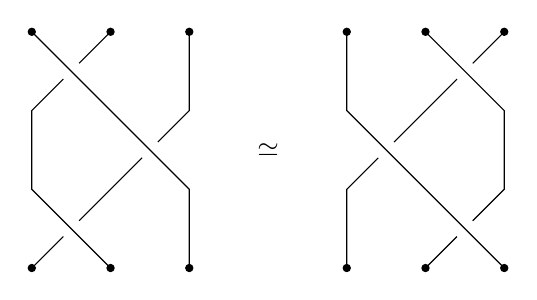
\begin{tikzpicture}
        \begin{scope}
            \draw[black,fill=black] (0, 0) circle (.3ex);
            \draw[black,fill=black] (1, 0) circle (.3ex);
            \draw[black,fill=black] (2, 0) circle (.3ex);
            \draw[black,fill=black] (0, 3) circle (.3ex);
            \draw[black,fill=black] (1, 3) circle (.3ex);
            \draw[black,fill=black] (2, 3) circle (.3ex);
            \draw (0, 3) -- (1, 2) -- (2, 1) -- (2, 0);
            \draw (1, 3) -- (0.6, 2.6);
            \draw (0.4, 2.4) -- (0, 2) -- (0, 1) -- (1, 0);
            \draw (2, 3) -- (2, 2) -- (1.6, 1.6);
            \draw (1.4, 1.4) -- (0.6, 0.6);
            \draw (0.4, 0.4) -- (0, 0);
        \end{scope}
        \node at (3cm,1.5cm) {$\simeq$};
        \begin{scope}[xshift=4cm]
            \draw[black,fill=black] (0, 0) circle (.3ex);
            \draw[black,fill=black] (1, 0) circle (.3ex);
            \draw[black,fill=black] (2, 0) circle (.3ex);
            \draw[black,fill=black] (0, 3) circle (.3ex);
            \draw[black,fill=black] (1, 3) circle (.3ex);
            \draw[black,fill=black] (2, 3) circle (.3ex);
            \draw (0, 3) -- (0, 2) -- (1, 1) -- (2, 0);
            \draw (1, 3) -- (2, 2) -- (2, 1) -- (1.6, 0.6);
            \draw (1.4, 0.4) -- (1, 0);
            \draw (2, 3) -- (1.6, 2.6);
            \draw (1.4, 2.4) -- (0.6, 1.6);
            \draw (0.4, 1.4) -- (0, 1) -- (0, 0);
        \end{scope}
    \end{tikzpicture} \]
    This relation precisely corresponds to the quantum Yang--Baxter equation.
\end{example}

\begin{topic}{chevalley-shephard-todd-theorem}{Chevalley--Shephard--Todd theorem}
    Let $V$ be a finite-dimensional \tref{LA:vector-space}{vector space} over a \tref{field}{field} $k$, and $G \subset \textup{GL}(V)$ a finite \tref{GT:group}{group} whose \tref{GT:order}{order} $|G|$ is invertible in $k$. An element $s \in \textup{GL}(V)$ is a \textit{pseudoreflection} if $s \ne 1$ and $s$ fixes a codimension $1$ subspace of $V$. The \textbf{Chevalley--Shephard--Todd theorem} states that the following are equivalent:
    \begin{enumerate}[label=(\roman*)]
        \item $G$ is generated by pseudoreflections,
        \item the ring of invariants $k[V]^G$ is a free polynomial algebra over $k$,
        \item $k[V]$ is a \tref{free-module}{free module} over $k[V]^G$.
    \end{enumerate}
\end{topic}

\begin{example}{chevalley-shephard-todd-theorem}
    Let $G = \ZZ/2\ZZ$ act on $V = k^2$ by $(x, y) \mapsto (x, -y)$. Then $G$ is generated by a pseudoreflection, and indeed
    \[ k[x, y]^G = k[x, y^2] \]
    a free polynomial algebra over $k$. However, if we let $G$ act on $V$ by $(x, y) \mapsto (-x, -y)$, then $G$ is not generated by pseudoreflections, and indeed
    \[ k[x, y]^G = k[x^2, xy, y^2] = k[u, v, w] / (w^2 - uv) \]
    is not a free polynomial algebra over $k$.
\end{example}

\begin{example}{chevalley-shephard-todd-theorem}
    Consider the \tref{GT:symmetric-group}{symmetric group} $S_n$ acting on $V = k^{n - 1}$ via the \tref{RT:standard-representation}{standard representation}. Note that any $2$-cycle acts by a pseudo-reflection, and since $S_n$ is generated by $2$-cycles, we can conclude that $k[V]^G$ is a free polynomial algebra over $k$.
\end{example}

\begin{topic}{molien-formula}{Molien's formula}
    Let $G$ be a finite \tref{GT:group}{group} and $\rho : G \to \textup{GL}(V)$ a finite-dimensional complex \tref{RT:representation}{representation}. Then $G$ acts naturally on the \tref{symmetric-algebra}{symmetric algebra} $\textup{Sym}(V)$. \textbf{Molien's formula} states that the \tref{hilbert-series}{Hilbert series} of the invariant subalgebra $\textup{Sym}(V)^G \subset \textup{Sym}(V)$ is given by
    \[ \textup{HS}_{\textup{Sym}(V)^G}(t) = \frac{1}{|G|} \sum_{g \in G} \frac{1}{\det(1 - gt)} . \]
\end{topic}

\begin{example}{molien-formula}
    \begin{proof}
        Write $S = \textup{Sym}(V)$. The \textit{Reynolds operator} $R^G : S \to S$ given by $f \mapsto \frac{1}{|G|} \sum_{g \in G} g \cdot f$ projects $S_d$ onto $S^G_d$ for each $d \ge 0$, so
        \[ \dim_\CC(S_d) = \tr_{S_d}(R^G) = \frac{1}{|G|} \sum_{g \in G} \tr_{S_d}(g) . \]
        % Hence, it suffices to show that 
        % \[ \sum_{d \ge 0} \tr_{S_d}(g) \cdot t^d = \frac{1}{\det(1 - gt)} \]
        % for all $g \in G$.
        Now fix $g \in G$, and let $\lambda_1, \ldots, \lambda_n$ be the eigenvalues of $\rho(g)$. Then the eigenvalues of $g$ acting on $S_d$ are given by $\mu_\alpha = \prod_{i = 1}^{n} \lambda_i^{\alpha_i}$ for each $\alpha \in \NN^n$ with $\alpha_1 + \ldots + \alpha_n = d$. Now it follows that
        \[ \sum_{d \ge 0} \tr_{S_d}(g) \cdot t^d = \sum_{\alpha} \prod_{i = 1}^{n} (\lambda_i t)^{\alpha_i} = \prod_{i = 1}^{n} \sum_{j \ge 0} (\lambda_i t)^j = \prod_{i = 1}^{n} \frac{1}{1 - \lambda_i t} = \frac{1}{\det(1 - gt)} . \]
        Combined with the above equation, the result follows.
    \end{proof}
\end{example}

\begin{topic}{domain}{domain}
    A non-zero \tref{ring}{commutative ring} $R$ is called a \textbf{domain} if it has no zero-divisors, that is, $ab = 0$ implies $a = 0$ or $b = 0$ for all $a, b \in R$.
\end{topic}

\begin{topic}{irreducible-element}{irreducible element}
    Let $R$ be a \tref{domain}{domain}. An element $a \in R$ is called a \textbf{irreducible} if $a$ is not a \tref{unit-element}{unit}, and for all $b, c \in R$ such that $bc = a$ either $b$ or $c$ is a unit.
\end{topic}

\begin{topic}{field}{field}
    A non-zero \tref{ring}{commutative ring} $R$ is called a \textbf{field} if all non-zero elements are units, that is, for all non-zero $a \in R$ there exists a $b \in R$ such that $ab = 1$. 
\end{topic}

\begin{example}{field}
    Every finite field has $p^n$ elements for some prime $p$ and integer $n \ge 1$, and conversely there exists, up to isomorphism, a unique finite field with $p^n$ elements.
    Namely, let $k$ be a field of $q$ elements. The \tref{prime-field}{prime field} of $k$ must be $\FF_p$ for some prime $p$, so $k$ is a finite-dimensional $\FF_p$-vector space, and hence $q = p^n$ for some $n \ge 1$. Note that $a^q - a = 0$ for all $a \in k$ since the units $k^*$ form a multiplicative group of order $q - 1$, so the polynomial $X^q - X$ factors as $\prod_{a \in k} (X - a)$ in $k$. In particular, $k$ is a \tref{splitting-field}{splitting field} of $X^q - X$ over $\FF_p$. The uniqueness claim now follows from the uniqueness of splitting fields.
    To show that for every $q = p^n$ there exists a field with $q$ elements, let $k$ be a splitting field of $X^q - X$ over $\FF_p$, and write $X^q - X = \prod_{i = 1}^{q} (X - \alpha_i)$ with $\alpha_i \in k$. Note that the derivative of $X^q - X$, which is $qX^{q - 1} - 1 = -1$, has no roots, so $X^q - X$ has no double roots, and hence the set $A = \{ \alpha_1, \ldots, \alpha_q \}$ has $q$ elements. Note that $0, \pm 1 \in A$ and $(\alpha_i + \alpha_j)^q = \alpha_i + \alpha_j$ and $(\alpha_i \alpha_j)^q = \alpha_i \alpha_j$ for all $i, j$, so $A$ is a subfield of $k$, and thus $k = \FF_p(\alpha_1, \ldots, \alpha_q) = A$ has $q$ elements, which proves the existence claim.
\end{example}

\begin{topic}{radical-ideal}{radical ideal}
    Let $R$ be a \tref{ring}{commutative ring}. The \textbf{radical} of an \tref{ideal}{ideal} $I \subset R$ is given by
    \[ \sqrt{I} = \{ x \in R \mid x^n \in I \} . \]
    An ideal $I$ is called \textbf{radical} if $I = \sqrt{I}$.
\end{topic}

\begin{topic}{prime-ideal}{prime ideal}
    Let $R$ be a \tref{ring}{commutative ring}. An \tref{ideal}{ideal} $I \subset R$ is called \textbf{prime} if $I \ne R$ and
    \[ ab \in I \implies a \in I \textup{ or } b \in I . \]
    Equivalently, $I \subset R$ is a prime ideal if and only if the quotient ring $R / I$ is a \tref{domain}{domain}.
\end{topic}

\begin{topic}{maximal-ideal}{maximal ideal}
    Let $R$ be a \tref{ring}{commutative ring}. An \tref{ideal}{ideal} $I \subset R$ is called \textbf{maximal} if $I \ne R$ and if $I \subset J \subsetneq R$ implies $I = J$ for any other ideal $J \subset R$.
    
    Equivalently, $I \subset R$ is a maximal ideal if and only if the quotient ring $R / I$ is a \tref{field}{field}.
    
    Every maximal ideal is \tref{prime-ideal}{prime}.
\end{topic}

\begin{example}{maximal-ideal}
    Every ideal $I \subsetneq R$ is contained in some maximal ideal $\mathfrak{m}$. Namely, consider the partially ordered set $P$ of ideals $J \subsetneq R$ containing $I$, ordered by inclusion. Then $P$ is non-empty as it contains $I$, and every chain $J_1 \subset J_2 \subset \ldots$ in $P$ has an upper bound $J = \cup_{i \ge 1} J_i$. Note that indeed $J$ is an ideal, and $J \ne R$ as $1 \not\in J$ because $1 \not\in J_i$ for all $i$.
    Now from \tref{GM:zorns-lemma}{Zorn's lemma} it follows $P$ has a maximal element, which corresponds to a maximal ideal $\mathfrak{m}$ containing $I$.
\end{example}

\begin{topic}{quotient-ring}{quotient ring}
    Given a \tref{ring}{commutative ring} $R$ and \tref{ideal}{ideal} $I$, the \textbf{quotient ring} $R/I$ is the ring
    \[ R/I = \{ a + I : a \in R \} \]
    where addition and multiplication are given by
    \[ (a + I) + (b + I) = (a + b) + I \quad \textup{ and } \quad (a + I) (b + I) = (ab) + I . \]
    It has the universal property that each morphism of rings $f \colon R \to S$ with $f(I) = 0$ uniquely extends to a morphism $R/I \to S$.
    \[ \svg \begin{tikzcd} R \arrow{r}{f} \arrow[swap]{d}{\pi} & S \\ R/I \arrow[dashed]{ur} & \end{tikzcd} \]
\end{topic}

\begin{topic}{local-ring}{local ring}
    A \tref{ring}{commutative ring} $R$ is \textbf{local} if it has exactly one \tref{maximal-ideal}{maximal ideal} $\mathfrak{m}$.
    
    The quotient $k = R/\mathfrak{m}$ is called the \textbf{residue field}.
\end{topic}

\begin{topic}{semi-local-ring}{semi-local ring}
    A \tref{ring}{commutative ring} $R$ is \textbf{semi-local} if it has finitely many \tref{maximal-ideal}{maximal ideals}.
\end{topic}

\begin{topic}{local-morphism}{local morphism}
    A \textbf{local morphism} of \tref{local-ring}{local rings} $f \colon R \to S$ is a ring morphism such that $f(\mathfrak{m}_R) \subset \mathfrak{m}_S$.
\end{topic}

\begin{topic}{finite-type}{finite type}
    Let $R$ and $S$ be \tref{ring}{commutative rings}. A \tref{ring-morphism}{ring morphism} $R \to S$ is said to be of \textbf{finite type} if $S$ is isomorphic to a quotient of $R[x_1, \ldots, x_n]$ for some integer $n$.
    
    That is, $S$ is a \tref{finitely-generated-algebra}{finitely generated $R$-algebra}.
\end{topic}

\begin{topic}{finitely-presented-algebra}{finitely presented algebra}
    Let $R$ and $S$ be \tref{ring}{commutative rings}. A \tref{ring-morphism}{ring morphism} $R \to S$ is said to be of \textbf{finite presentation} if $S$ is isomorphic to $R[x_1, \ldots, x_n] / (f_1, \ldots, f_m)$ for some integer $n$ and some $f_i \in R[x_1, \ldots, x_n]$.
    
    In this case, $S$ is also said to be a \textbf{finitely presented $R$-algebra}.
\end{topic}

\begin{example}{finitely-presented-algebra}
    Let $R = k[x_1, x_2, \ldots]$ and $S = R / (x_1^2, x_2^2, \ldots)$. Then the quotient map $R \to S$ is of \tref{finite-type}{finite type}, but not of finite presentation.
\end{example}

\begin{topic}{krull-dimension}{Krull dimension}
    The \textbf{Krull dimension} of a \tref{ring}{commutative ring} $R$ is the supremum of the lengths of all chains of \tref{prime-ideal}{prime ideals}, where a chain of the form
    \[ \mathfrak{p}_0 \subsetneq \mathfrak{p}_1 \subsetneq \cdots \subsetneq \mathfrak{p}_n \]
    has length $n$.
\end{topic}

\begin{topic}{chinese-remainder-theorem}{Chinese remainder theorem}
    Let $R$ be a \tref{ring}{commutative ring} and suppose $I, J$ are coprime ideals of $R$, i.e. $I + J = R$. Then the \textbf{Chinese remainder theorem} states that $I \cap J = I \cdot J$ and that there is an isomorphism of rings
    \[ R / (I \cdot J) \xrightarrow{\sim} (R / I) \times (R/J), \qquad a \mod (I \cdot J) \mapsto (a \mod I, b \mod J) . \]
    In particular, when $R = \ZZ$ with $I = (n)$ and $J = (m)$ for $n, m$ relatively prime, there is
    \[ \ZZ / nm \ZZ \isom (\ZZ/n\ZZ) \times (\ZZ/m\ZZ), \qquad a \mod nm \mapsto (a \mod n, a \mod m) . \]
\end{topic}

\begin{topic}{dual-numbers}{dual numbers}
    Let $R$ be a \tref{ring}{commutative ring}. The \textbf{ring of dual numbers} over $R$ is the quotient ring
    \[ R[\varepsilon] / (\varepsilon^2) . \]
\end{topic}

\begin{topic}{noetherian-ring}{noetherian ring}
    A \tref{ring}{commutative ring} $R$ is called \textbf{noetherian} if it satisfies the \textit{ascending chain condition}: for any increasing sequence of ideals
    \[ I_1 \subset I_2 \subset I_3 \subset \cdots \]
    there exists some $N \in \NN$ such that $I_n = I_N$ for any $n \ge N$.
    
    Equivalently, $R$ is noetherian if all its ideals are finitely generated.
\end{topic}

\begin{example}{noetherian-ring}
    The following are all noetherian rings.
    \begin{itemize}
        \item Any \tref{field}{field}: their only ideal is $(0)$.
        \item Any \tref{principal-ideal-domain}{PID}: every ideal is generated by a single element.
        \item If $R$ is noetherian, then so is $R[x]$: this is \textit{Hilbert's basis theorem}.
    \end{itemize}
\end{example}

\begin{example}{noetherian-ring}
    The ring $k[x_1, x_2, x_3, \ldots]$ is not noetherian. Namely, the sequence of ideals
    \[ (x_1) \subset (x_1, x_2) \subset (x_1, x_2, x_3) \subset \ldots \]
    is ascending, but does not stabilize.
\end{example}

\begin{topic}{localization}{localization}
    Let $R$ be a \tref{ring}{commutative ring}, and $S \subset R$ a \textit{multiplicative set} (that is, $1 \in S$ and $xy \in S$ for all $x, y \in S$). Then the \textbf{localization} of $R$ w.r.t. $S$ is the ring
    \[ S^{-1} R = R \times S / \sim{} \quad \textup{ where } (r_1, s_1) \sim{} (r_2, s_2) \textup{ if } t(r_1 s_2 - r_2 s_1) = 0 \textup{ for some } t \in S . \]
\end{topic}

\begin{example}{localization}
    If $R$ is a \tref{domain}{domain}, then $S = R - \{ 0 \}$ is a multiplicative set, and $S^{-1} R$ is the \tref{field-of-fractions}{field of fractions} of $R$.
\end{example}

\begin{example}{localization}
    For any commutative ring $R$ and $f \in R$, the set
    \[ S = \{ 1, f, f^2, \ldots \} \]
    is a multiplicative set, and the localization is
    \[ R_f := S^{-1} R = \left\{ \frac{a}{f^n} : a \in R, \; n \ge 0 \right\} . \]
\end{example}

\begin{example}{localization}
    For any commutative ring $R$ and \tref{prime-ideal}{prime ideal} $\mathfrak{p}$, the set
    \[ S = \{ f \in R \mid f \not\in \mathfrak{p} \} \]
    is a multiplicative set, and the localization
    \[ R_\mathfrak{p} := S^{-1} R = \left\{ \frac{f}{g} : f, g \in R, \; g \not\in \mathfrak{p} \right\} \]
    is a \tref{local-ring}{local ring} with maximal ideal $\mathfrak{p} R_\mathfrak{p}$.
\end{example}

\begin{topic}{total-quotient-ring}{total quotient ring}
    The \textbf{total quotient ring} of a \tref{ring}{commutative ring} $R$ is the \tref{localization}{localization} $S^{-1} R$, with $S$ the set of elements of $R$ which are not \tref{zero-divisor}{zero-divisors}.
    
    When $R$ is a \tref{domain}{domain}, this construction gives the \tref{field-of-fractions}{field of fractions} of $R$.
\end{topic}

\begin{topic}{regular-ring}{regular (local) ring}
    A \textbf{regular local ring} is a commutative \tref{noetherian-ring}{noetherian} \tref{local-ring}{local} ring such that the minimal number of generators of its maximal ideal is equal to its \tref{krull-dimension}{Krull dimension}. Equivalently, a local ring $R$ with maximal ideal $\mathfrak{m}$ and residue field $k = R / \mathfrak{m}$ is regular if and only if $\dim_k(\mathfrak{m} / \mathfrak{m}^2) = \dim R$.
    
    A \textbf{regular ring} is a commutative noetherian ring, such that the \tref{localization}{localization} at every \tref{prime-ideal}{prime ideal} is a regular local ring.
\end{topic}

\begin{example}{regular-ring}
    Every field is a regular local ring: their Krull dimension is zero, and their maximal ideal is $(0)$.
\end{example}

\begin{example}{regular-ring}
    \begin{itemize}
        \item The local ring $R = k[x]/(x^2)$ is not a regular local ring. Its only prime ideal is its maximal ideal $\mathfrak{m} = (x)/(x^2)$, so the Krull dimension is zero, but the minimal number of generators of $\mathfrak{m}$ is one.
        \item The ring $R = k[x, y]/(y^2 - x^3)$ is not regular. Namely, at the maximal ideal $\mathfrak{m} = (x, y)$ we have $\dim R_\mathfrak{m} = 1$ since the only non-zero prime ideal in $R$ is $\mathfrak{m}$. However, $\dim_k(\mathfrak{m} / \mathfrak{m}^2) = \dim_k(k \cdot x \oplus k \cdot y) = 2$.
    \end{itemize}
\end{example}

\begin{topic}{principal-ideal-domain}{principal ideal domain (PID)}
    A \textbf{principal ideal domain} (PID) is a \tref{domain}{domain} $R$ in which every \tref{ideal}{ideal} is \tref{principal-ideal}{principal}. That is, every ideal $I \subset R$ is of the form $I = (x)$ for some element $x \in R$.
\end{topic}

\begin{topic}{unique-factorization-domain}{unique factorization domain (UFD)}
    A \textbf{unique factorization domain} (UFD) is a \tref{domain}{domain} $R$ for which every non-zero $x \in R$ can be written as the product of a \tref{unit-element}{unit} and a finite number of \tref{irreducible-element}{irreducible} elements:
    \[ a = u \cdot p_1 \cdot p_2 \cdot \cdots \cdot p_k \qquad u \in R^\times, \; k \ge 0, \; p_i \in R \textup{ irreducible}. \]
\end{topic}

\begin{topic}{euclidean-ring}{Euclidean ring}
    A \textbf{Euclidean ring} is a \tref{domain}{domain} $R$ for which there exists a function
    \[ g \colon R^\times \to \ZZ_{\ge 0} \]
    such that for all $a, b \in R$ with $b \ne 0$, there exists $q, r \in R$ with $a = qb + r$ and either $r = 0$ or $g(r) < g(b)$.
    
    That is, a ring in which one can perform division with remainder. The function $g$ is used to say that the `remainder' $r$ is `smaller' than the element $b$ one divides by.
    
    In particular, one can find the \textit{gcd} of elements by means of the \textit{Euclidean algorithm}.
\end{topic}

\begin{topic}{field-of-fractions}{field of fractions}
    The \textbf{field of fractions} of a \tref{domain}{domain} $R$ is the \tref{field}{field} given by
    \[ K = \left\{ (a, b) : a, b \in R, b \ne 0 \right\} / \sim{} \]
    where $(a, b) \sim{} (c, d)$ if and only if $ad = bc$. Indeed $(a, b)$ represents the fraction $\frac{a}{b}$. Addition and multiplication are given by
    \[ \frac{a}{b} + \frac{c}{d} = \frac{ad + bc}{bd} \quad \textup{ and } \quad \frac{a}{b} \cdot \frac{c}{d} = \frac{ac}{bd} . \]
\end{topic}

\begin{example}{field-of-fractions}
    The field of fractions of $\ZZ$ is $\QQ$.
\end{example}

\begin{topic}{valuation-ring}{valuation ring}
    A \textbf{valuation ring} is a \tref{domain}{domain} $R$ such that for every element $x$ of its \tref{field-of-fractions}{field of fractions}, at least one of $x$ or $x^{-1}$ belongs to $R$.
\end{topic}

\begin{example}{valuation-ring}
    Let $\phi \colon K \to \RR_{\ge 0}$ be a \tref{NT:archimedean-valuation}{non-archimedean} \tref{NT:valuation}{valuation} on a field $K$. Then the subring
    \[ A = \{ x \in K \mid \phi(x) \le 1 \} \]
    is a valuation ring, called the \textit{valuation ring} of $\phi$. Indeed, for every $x \in K$, we have $x \in A$ if $\phi(x) \le 1$ and $x^{-1} \in A$ if $\phi(x) > 1$. In particular, the field of fractions of $A$ is $K$. The valuation ring $A$ is a \tref{local-ring}{local ring} with unit group $A^* = \{ x \in K \mid \phi(x) = 1 \}$ and maximal ideal $\mathfrak{m} = \{ x \in K \mid \phi(x) < 1 \}$.
\end{example}

\begin{topic}{discrete-valuation-ring}{discrete valuation ring}
    A domain \tref{domain}{domain} $R$ is a \textbf{discrete valuation ring} if there is a \textit{discrete valuation} $\nu$ of its \tref{field-of-fractions}{field of fractions} $K$, such that $R$ is the \textit{valuation ring} of $v$. This means there is a homomorphism
    \[ \nu \colon K^\times \to \ZZ \]
    such that
    \[ R = \{ x \in K \mid \nu(x) \ge 0 \} . \]
    
    In particular, $R$ is \tref{local-ring}{local} with maximal ideal $\mathfrak{m} = \{ x \in K \mid \nu(x) > 0 \}$. Indeed, any element $x \in R$ with $\nu(x) = 0$ is a unit in $R$.
\end{topic}

\begin{example}{discrete-valuation-ring}
    Let $K = \QQ$ and fix a prime number $p$. Any non-zero $x \in \QQ$ can be written uniquely as $x = p^m y$ where $k \in \ZZ$ and both the numerator and denominator of $y$ are coprime to $p$. Now define the discrete valuation $\nu_p(x) = m$, then the valuation ring is the local ring $\ZZ_{(p)}$.
\end{example}

\begin{topic}{monic-polynomial}{monic polynomial}
    Let $k$ be a \tref{ring}{commutative ring}. A polynomial $f \in k[x]$ is called \textbf{monic} if its leading coefficient is $1$.
\end{topic}

\begin{topic}{integral-element}{integral element}
    Let $A$ be a \tref{ring}{commutative ring}, and $B$ an $A$-algebra. An element $x \in B$ is said to be \textbf{integral} over $A$ if $x$ is a root of a monic polynomial with coefficients in $A$. That is,
    \[ x^n + a_1 x^{n - 1} + \cdots + a_n = 0 \]
    for some $a_i \in A$.
\end{topic}

\begin{topic}{integral-closure}{integral closure}
    Let $A$ be a \tref{ring}{commutative ring}, and $B$ an $A$-algebra. The \textbf{integral closure} of $A$ in $B$ is the subring of $B$ of elements which are \tref{integral-element}{integral} over $A$.
    
    If the integral closure is equal to $A$, then $A$ is said to be \textbf{integrally closed} in $B$. If the integral closure is equal to $B$, the ring $B$ is said to be \textbf{integral} over $A$.
\end{topic}

\begin{topic}{artin-ring}{artin ring}
    A \tref{ring}{commutative ring} $R$ is called \textbf{artin} if it satisfies the \textit{descending chain condition}: for any decreasing sequence of ideals
    \[ I_1 \supset I_2 \supset I_3 \supset \cdots \]
    there exists some $N \in \NN$ such that $I_n = I_N$ for any $n \ge N$.
\end{topic}

\begin{example}{artin-ring}
    The ring $R = k[x] / (x^n)$, for a \tref{field}{field} $k$ and integer $n \ge 0$, is artin. Namely, the only ideals of $R$ are of the form $(x^k)$ with $0 \le k \le n$. 
\end{example}

\begin{topic}{fractional-ideal}{fractional ideal}
    Let $R$ be a \tref{domain}{domain} and $K$ its \tref{field-of-fractions}{field of fractions}. A \textbf{fractional ideal} of $R$ is an $R$-submodule $M$ of $K$ such that $xM \subset R$ for some non-zero $x \in R$.
\end{topic}

\begin{topic}{invertible-ideal}{invertible ideal}
    Let $R$ be a \tref{domain}{domain} and $K$ its \tref{field-of-fractions}{field of fractions}. An $R$-submodule $M$ of $K$ is an \textbf{invertible ideal} if there exists a submodule $N$ of $K$ such that $MN = R$. This module $N$ is then unique and equal to
    \[ N = (R : M) := \{ x \in K \mid xM \subset R \} . \]
    The invertible ideals form a group with respect to multiplication, whose unit element is $R = (1)$.
\end{topic}

\begin{topic}{quotient-ideal}{quotient ideal}
    Let $R$ be a \tref{ring}{commutative ring}, and $I, J \subset R$ two \tref{ideal}{ideals}. Their \textbf{quotient ideal} is the ideal
    \[ (I : J) = \{ x \in R \mid xJ \subset I \} . \]
\end{topic}

\begin{example}{quotient-ideal}
    \begin{itemize}
        \item In $\ZZ$, we have $((6) : (2)) = (3)$.
        \item In $k[x, y]$, we have $((xy), (x)) = (y)$.
    \end{itemize}
\end{example}

\begin{topic}{divisorial-ideal}{divisorial ideal}
    Let $R$ be a \tref{domain}{domain}. A \textbf{divisorial ideal} of $R$ is a \tref{fractional-ideal}{fractional ideal} $I$ of $R$ such that
    \[ I = (R : (R : I)) , \]
    where $(I : J) = \{ x \in K \mid xJ \subset I \}$.
\end{topic}

\begin{topic}{syzygy-module}{syzygy module}
    Let $R$ be a \tref{ring}{commutative ring} and let $M$ be a \tref{module}{module} over $R$. The \textbf{(first) syzygy module} $\operatorname{Syz}(f_1, \ldots, f_n)$ of generators $f_1, \ldots, f_n \in M$ is the $R$-module consisting of all relations between these elements, that is, it is the kernel of
    \[ \bigoplus_{i = 1}^{n} R \to M, \qquad (r_1, \ldots, r_k) \mapsto r_1 f_1 + \cdots r_n f_n . \]
    Inductively, one can define the $i$-th syzygy module for any $i \ge 2$ after choosing generators for the $(i - 1)$-th syzygy module.
\end{topic}

% Hilbert's three theorems
\begin{topic}{hilbert-basis-theorem}{Hilbert's basis theorem}
    \textbf{Hilbert's basis theorem} states that if a \tref{ring}{commutative ring} $R$ is \tref{noetherian-ring}{noetherian}, then so is the polynomial ring $R[x]$.
\end{topic}

\begin{topic}{hilbert-nullstellensatz}{Hilbert's Nullstellensatz}
    Let $k$ be an \tref{algebraically-closed-field}{algebraically closed field} and $A = k[x_1, \ldots, x_n]$ for some $n \ge 0$. For any subset $S \subset A$, let
    \[ Z(S) = \{ p \in \AA^n \mid f(p) = 0 \textup{ for all } f \in S \} , \]
    which is a closed subset of $\AA^n_k = \Spec A$. Conversely, for any subset $Y \subset \AA^n_k$, let
    \[ I(Y) = \{ f \in A \mid f(p) = 0 \textup{ for all } p \in Y \} , \]
    which is a \tref{radical-ideal}{radical ideal} of $A$.
    \textbf{Hilbert's Nullstellensatz} states that $Z$ and $I$, when restricted to the set of radical ideals of $A$ and the set of closed subsets of $\AA^n_k$, are inverses of each other. Moreover, they reverse the partial orderings on these sets given by inclusion: $I \subset J$ if and only if $Z(I) \supset Z(J)$ for all radical ideals $I$ and $J$ of $A$.
\end{topic}

\begin{topic}{hilbert-syzygy-theorem}{Hilbert's syzygy theorem}
    \textbf{Hilbert's syzygy theorem} states that if $M$ is a finitely generated module over a polynomial ring $k[x_1, \ldots, x_n]$, then the $n$-th \tref{syzygy-module}{syzygy module} $M$ is always \tref{free-module}{free}.
    
    In particular, this implies that there exists a free resolution
    \[ 0 \to F_k \to F_{k - 1} \to \cdots \to F_0 \to M \to 0 \]
    of length $k \le n$.
\end{topic}

\begin{topic}{primary-ideal}{primary ideal}
    Let $R$ be a \tref{ring}{commutative ring}. An \tref{ideal}{ideal} $\mathfrak{q}$ of $R$ is \textbf{primary} if $\mathfrak{q} \ne R$ and if
    \[ xy \in \mathfrak{q} \implies \textup{ either } x \in \mathfrak{q} \textup{ or } y^n \in \mathfrak{q} \textup{ for some } n > 0 . \]
    In other words,
    \[ \mathfrak{q} \textup{ is primary } \iff A / \mathfrak{q} \ne 0 \textup{ and every zero-divisor in } A / \mathfrak{q} \textup{ is nilpotent} . \]
\end{topic}

\begin{topic}{primary-decomposition}{primary decomposition}
    Let $R$ be a \tref{ring}{commutative ring}. A \textbf{primary decomposition} of an ideal $I \subset R$ is an expression of $I$ as a finite intersection of \tref{primary-ideal}{primary ideals},
    \[ I = \bigcap_{i = 1}^{n} \mathfrak{q}_i . \]
    The primary decomposition is said to be \textbf{minimal} if (i) the $\mathfrak{p}_i = r(\mathfrak{q}_i)$ are all distinct, and (ii) no $\mathfrak{q}_i$ contains the intersection of the other primary ideals.
\end{topic}

\begin{topic}{annihilator}{annihilator}
    Let $R$ be a \tref{ring}{commutative ring} and $M$ an $R$-module. The \textbf{annihilator} of $M$ is the \tref{ideal}{ideal} of $R$ given by
    \[ \operatorname{Ann}_R(M) = \{ x \in R \mid xM = 0 \} . \]
\end{topic}

\begin{topic}{nilradical}{nilradical}
     The \textbf{nilradical} of a \tref{ring}{commutative ring} $R$ is the ideal of \tref{nilpotent-element}{nilpotent} elements
     \[ \mathfrak{N}_R = \{ x \in R \mid x \textup{ is nilpotent } \} . \]
     It is equal to the intersection of all prime ideals of $R$,
     \[ \mathfrak{N}_R = \bigcap_{\mathfrak{p} \subset R \textup{ prime}} \mathfrak{p} . \]
\end{topic}

\begin{topic}{jacobson-radical}{Jacobson radical}
     The \textbf{Jacobson radical} of a \tref{ring}{commutative ring} $R$ is the ideal given by the intersection of all \tref{maximal-ideal}{maximal} ideals,
     \[ \mathfrak{J}_R = \bigcap_{\mathfrak{m} \subset R \textup{ maximal}} \mathfrak{m} . \]
     It can also be characterized by
     \[ x \in \mathfrak{J}_R \iff 1 - xy \textup{ is a unit for all } y \in R . \]
\end{topic}

\begin{topic}{regular-sequence}{regular sequence}
    Let $R$ be a \tref{ring}{commutative ring}, and $M$ an $R$-module. An $M$-\textbf{regular sequence} is a sequence
    \[ r_1, r_2, \ldots, r_d \in R \]
    such that $r_i$ is not a \textit{zero-divisor} on $M/(r_1, \ldots, r_{i - 1})$. That is, if $r_i m = 0$ for some $m \in M / (r_1, \ldots, r_{i - 1})$, then $m = 0$.
    
    When $M = R$, such a sequence is simply called a \textbf{regular sequence}.
\end{topic}

\begin{example}{regular-sequence}
    Consider $R = k[x, y]$ and the sequence $(xy, x^2)$. This sequence is not regular, since $x^2 \cdot y = 0$ in $\QQ[x, y] / (xy)$, although $y \ne 0$.
\end{example}

\begin{example}{regular-sequence}
    Consider $R = k[x, y, z]$ and the sequence $(x, y(1 - x), z(1 - x))$. This sequence is regular since
    \[ y(1 - x) = y \in k[x, y, z]/(x) = k[y, z] \quad \textup{ and } \quad z(1 - x) = z \in k[x, y, z]/(x, y - xy) = k[z] \]
    are both non-zero-divisors.
    
    However, note that the order matters as $(y(1 - x), z(1 - x), x)$ is not a regular sequence. Namely, $z(1 - x) \cdot y = 0 \in k[x, y, z] / (y(1 - x))$ even though $y \ne 0$.
\end{example}

\begin{topic}{hilbert-series}{Hilbert series}
    Let $S = \bigoplus_{i \ge 0} S_i$ be a \tref{finitely-generated-algebra}{finitely generated} \tref{graded-ring}{graded} commutative algebra over a field $k$, with $S_0 = k$. The \textbf{Hilbert series} of $S$ is defined as
    \[ \operatorname{HS}_S(t) = \sum_{i = 0}^{\infty} \dim_k S_i \cdot t^i . \]
\end{topic}

\begin{example}{hilbert-series}
    Let $R = k[x_1, \ldots, x_n]$ and $I = (f)$ for some homogenous polynomial of degree $d$. Then we have an exact sequence (a free resolution)
    \[ 0 \to R(-d) \xrightarrow{\cdot f} R \to R / I \to 0 , \]
    which implies that
    \[ \operatorname{HS}_{R/I}(t) = \operatorname{H}_R(t) - \operatorname{HS}_{R(-d)}(t) = \operatorname{HS}_R(t) (1 - t^d) = \frac{1 - t^d}{(1 - t)^n}. \]
\end{example}

\begin{topic}{hilbert-polynomial}{Hilbert polynomial}
    Let $S = \bigoplus_{i \ge 0} S_i$ be a \tref{finitely-generated-algebra}{finitely generated} graded commutative \tref{algebra}{algebra} over a \tref{field}{field} $k$, with $S_0 = k$. The \textit{Hilbert function}
    \[ i \mapsto \dim_k S_i \]
    becomes polynomial for large enough values of $i$, and the resulting polynomial is called the \textbf{Hilbert polynomial} $\operatorname{HP}_S(i)$ of $S$.
\end{topic}

\begin{example}{hilbert-polynomial}
    Let $R = k[x_1, \ldots, x_n]$, then
    \[ \dim R_i = \binom{n - 1 + i}{i} = \frac{(n - 1 + i) \cdots (i + 1)}{(n - 1)!} , \]
    which is a polynomial in $i$ for every value of $n$. In particular,
    \[ \begin{aligned}
        \operatorname{HP}_{k[x]}(i) &= 1, \\
        \operatorname{HP}_{k[x, y]}(i) &= i + 1, \\
        \operatorname{HP}_{k[x, y, z]}(i) &= \tfrac{1}{2} (i + 1)(i + 2), \\
        \operatorname{HP}_{k[x, y, z, w]}(i) &= \tfrac{1}{6} (i + 1)(i + 2)(i + 3) .
    \end{aligned} \]
\end{example}

\begin{example}{hilbert-polynomial}
    Let $R = k[x, y, z] / (z^2 - xy)$. It is easy to see that
    \[ \dim R_i = \left\{ \begin{array}{cl}
        1 & \textup{ if } i = 0, \\
        3 & \textup{ if } i = 1, \\
        i + 1 & \textup{ otherwise}.
    \end{array} \right. \]
    Hence, $\operatorname{HP}_R(i) = i + 1$.
\end{example}

\begin{topic}{absolutely-flat-ring}{absolutely flat ring}
    A \tref{ring}{commutative ring} $R$ is called \textbf{absolutely flat} if every $R$-module is \tref{flat-module}{flat}.
\end{topic}

\begin{topic}{standard-smooth-algebra}{standard smooth algebra}
    Let $A$ be \tref{ring}{commutative ring}, and $B = A[x_1, \ldots, x_n] / (f_1, \ldots, f_c)$ a \tref{finitely-presented-algebra}{finitely presented $A$-algebra}. Then $B$ is a \textbf{standard smooth} over $A$ if the determinant
    \[ \det \begin{pmatrix}
        \frac{\partial f_1}{\partial x_1} & \frac{\partial f_1}{\partial x_2} & \cdots & \frac{\partial f_1}{\partial x_c} \\
        \frac{\partial f_2}{\partial x_1} & \frac{\partial f_2}{\partial x_2} & \cdots & \frac{\partial f_2}{\partial x_c} \\ 
        \vdots & \vdots & \ddots & \vdots \\ 
        \frac{\partial f_c}{\partial x_1} & \frac{\partial f_c}{\partial x_2} & \cdots & \frac{\partial f_c}{\partial x_c}
    \end{pmatrix} \]
    maps to an invertible element in $B$. Note that this definition is dependent on the presentation of $B$.
\end{topic}

\begin{example}{standard-smooth-algebra}
    \begin{itemize}
        \item Take $A = k$ a field and $B = k[x, y] / (xy)$. Then $\partial (xy) / \partial x = y$ which is not invertible in $B$, so $k[x, y] / (xy)$ is not standard smooth over $k$.
        \item Taking $B = k[x, y] / (xy - 1)$, we see that $\partial (xy - 1) / \partial x = y$, which is invertible in $B$. Hence $k[x, y] / (xy - 1)$ is standard smooth over $k$.
    \end{itemize}
\end{example}

\begin{topic}{standard-etale-algebra}{standard étale algebra}
    Let $R$ be \tref{ring}{commutative ring}. A \textbf{standard étale algebra} over $R$ is an \tref{algebra}{$R$-algebra} of the form
    \[ R[x]_g / (f) , \]
    where $f, g \in R[x]$ with $f$ monic and the derivative $f'$ is invertible in the \tref{localization}{localization} $R[x]_g$.
\end{topic}

\begin{example}{standard-etale-algebra}
    Let $k$ be a field, and $n \ge 1$ an integer with $n \nmid \operatorname{char}(k)$. Then $k[t^{\pm 1}, x] / (x^n - t)$ is a standard étale algebra over $k[t^{\pm 1}]$, with $f = x^n - t$ and $g = 1$ as in the definition. Indeed, $f' = n x^{n - 1}$ has inverse $\tfrac{1}{n} x t^{-1}$ in $k[t^{\pm 1}, x]$.
    
    However, the algebra $k[t, x] / (x^n - t)$ over $k[t]$ is not standard étale, with $f = x^n - t$ and $g = 1$ as in the definition. Indeed, the derivative $f' = n x^{n - 1}$ is not invertible in $k[t, x] / (x^n - t)$.
\end{example}

\begin{topic}{etale-algebra}{étale algebra}
    Let $A$ be a \tref{ring}{commutative ring} and $B$ an $A$-algebra. Then $B$ is an \textbf{étale algebra} over $A$ if $B$ is a \tref{flat-module}{flat} $A$-module and $\Omega_{B/A} = 0$.
\end{topic}

\begin{topic}{fitting-ideal}{Fitting ideal}
    Let $R$ be a \tref{ring}{commutative ring} and $M$ an $R$-\tref{module}{module} generated by elements $m_1, \ldots, m_n \in M$, with relations
    \[ a_{i1} m_1 + \cdots a_{in} m_n = 0 \textup{ for } i = 1, 2, \ldots, \ell . \]
    Then the \textbf{$i$-th Fitting ideal} $\operatorname{Fitt}_i(M)$ of $M$ is generated by the minors (determinants of submatrices) of order $n - i$ of the matrix $a_{ij}$. It can be shown that this does not depend on the choice of generators or relations. One has the inclusions
    \[ \operatorname{Fitt}_0(M) \subset \operatorname{Fitt}_1(M) \subset \operatorname{Fitt}_2(M) \subset \cdots \]
    Intuitively, the $i$-th fitting ideal (or actually the quotient $R / \operatorname{Fitt}_i(M)$) measures the obstruction for $M$ to be generated by $i$ elements.
    
    Sometimes the \textbf{Fitting ideal} of $M$ is defined as the first non-zero fitting ideal.
\end{topic}

\begin{example}{fitting-ideal}
    If $M$ is \tref{free-module}{free} of rank $n$, the matrix $a_{ij}$ will be of size $0 \times n$. Hence $\operatorname{Fitt}_i(M) = 0$ for $i < n$ as there are no submatrices of size $n - i > 0$, and $\operatorname{Fitt}_i(M) = R$ for $i \ge n$ as the determinant of a $0 \times 0$ matrix is one.
\end{example}

\begin{example}{fitting-ideal}
    Consider $M = \ZZ / p \ZZ \times \ZZ / p^2 \ZZ$ as $\ZZ$-module. It can be generated by $m_1 = (1, 0)$ and $m_2 = (0, 1)$ with relations $p m_1 = 0$ and $p^2 m_2 = 0$, so the corresponding matrix is
    \[ a_{ij} = \begin{pmatrix} p & 0 \\ 0 & p^2 \end{pmatrix} \]
    and thus
    \[ \operatorname{Fitt}_0(M) = (p^3), \quad \operatorname{Fitt}_1(M) = (p, p^2) = (p) \quad \textup{ and } \quad \operatorname{Fitt}_{\ge 2}(M) = \ZZ . \]
\end{example}

\begin{example}{fitting-ideal}
    Consider the finitely generated abelian group $M = \ZZ^r \times \ZZ / d_1 \ZZ \times \cdots \times \ZZ / d_k \ZZ$ with $d_1 | d_2 | \cdots | d_k$. Using the natural generators, the relation matrix is
    \[ a_{ij} = \begin{pmatrix} \textbf{0}_{r \times r} & & &  \\  & d_1 & \\ & & \ddots & \\ & & & d_k \end{pmatrix} \]
    and thus
    \[ \begin{array}{rcl}
         \operatorname{Fitt}_{0 \le i \le r}(M) &=& (0) , \\
        \operatorname{Fitt}_{r + 1}(M) &=& (d_1 d_2\cdots d_k) , \\
        \operatorname{Fitt}_{r + 2}(M) &=& (d_1 d_2\cdots d_{k - 1}) , \\
        & \vdots & \\
        \operatorname{Fitt}_{r + k - 1}(M) &=& (d_1) , \\
        \operatorname{Fitt}_{\ge r + k}(M) &=& \ZZ .
    \end{array} \]
\end{example}

\begin{example}{fitting-ideal}
    Consider the scheme $X = \Spec k[x_1, \ldots, x_n] / I$ with $I = (f_1, \ldots, f_k)$ for some polynomials $f_i$. The module of differentials
    \[ \Omega_{X/k} = \left(\bigoplus_{i = 1}^{n} k[x_1, \ldots, x_n] / I \cdot dx_i \right) / (df_1, df_2, \ldots, df_k) \]
    is generated by $dx_1, \ldots, dx_n$ and relations
    \[ df_i = \sum_{j = 1}^{n} \frac{\partial f_i}{\partial x_j} dx_j = 0 \quad \textup{ for } i = 1, 2, \ldots, k , \]
    so the corresponding matrix is the Jacobian matrix
    \[ J = \begin{pmatrix}
        \frac{\partial f_1}{\partial x_1} & \frac{\partial f_1}{\partial x_2} & \cdots & \frac{\partial f_1}{\partial x_n} \\
        \frac{\partial f_2}{\partial x_1} & \frac{\partial f_2}{\partial x_2} & \cdots & \frac{\partial f_2}{\partial x_n} \\
        \vdots & \vdots & \ddots & \vdots \\
        \frac{\partial f_k}{\partial x_1} & \frac{\partial f_k}{\partial x_2} & \cdots & \frac{\partial f_k}{\partial x_n}
    \end{pmatrix} . \]
    Now $X$ is smooth over $k$ if and only if $\Omega_{X/k}$ is locally free of rank $n = \dim X$, which is equivalent to the Fitting ideal $\operatorname{Fitt}_{\dim X}(\Omega_{X/k})$ generating the unit ideal in the localization of each prime ideal of $k[x_1, \ldots, x_n] / I$, which is equivalent to the Fitting ideal $\operatorname{Fitt}_{\dim X}(\Omega_{X/k})$ generating the unit ideal in $k[x_1, \ldots, x_n] / I$ itself.
\end{example}

\begin{topic}{gcd}{greatest common divisor (GCD)}
    Let $R$ be a \tref{ring}{commutative ring}. A \textbf{greatest common divisor} of two elements $a, b \in R$ is an element $d \in R$ such that $d | a, b$ and for any other $d' \in R$ with $d' | a, b$ one has $d' | d$. It is denoted $d = \operatorname{gcd}(a, b)$.
\end{topic}

\begin{topic}{lcm}{least common multiple (LCM)}
    Let $R$ be a \tref{ring}{commutative ring}. A \textbf{least common multiple} of two elements $a, b \in R$ is an element $m \in R$ such that $a, b | m$ and for any other $m' \in R$ with $a, b | m$ one has $m | m'$. It is denoted $m = \operatorname{lcm}(a, b)$.
\end{topic}

\begin{topic}{gcd-domain}{GCD domain}
    A \textbf{GCD domain} is a \tref{domain}{domain} $R$ in which any two elements $a, b$ have a \tref{gcd}{greatest common divisor}.
\end{topic}

\begin{topic}{gorenstein-ring}{Gorenstein ring}
    A \textbf{Gorenstein local ring} is a commutative \tref{noetherian-ring}{noetherian} \tref{local-ring}{local} \tref{ring}{ring} $R$ with finite \tref{injective-dimension}{injective dimension} as an $R$-module.
    
    A \textbf{Gorenstein ring} is a commutative noetherian ring $R$ such that the localization $R_\mathfrak{p}$ is Gorenstein for each \tref{prime-ideal}{prime ideal} $\mathfrak{p}$.
\end{topic}

\begin{topic}{cohen-macaulay-ring}{Cohen--Macaulay ring}
    A \tref{finitely-generated-module}{finitely generated} \tref{module}{module} $M$ over a commutative \tref{noetherian-ring}{noetherian} \tref{local-ring}{local} \tref{ring}{ring} $R$ is \textbf{Cohen--Macaulay} if its \tref{depth-module}{depth} $\operatorname{depth}_{\mathfrak{m}}(M)$ equals its \tref{krull-dimension}{dimension} $\dim_R(M) := \dim(R/\operatorname{Ann}_R(M))$.
    
    More generally, for a commutative noetherian ring $R$, a finitely generated $R$-module $M$ is \textbf{Cohen--Macaulay} if the localization $M_\mathfrak{m}$ is Cohen--Macaulay over $R_\mathfrak{m}$ for each maximal ideal $\mathfrak{m}$ of $R$.
    
    A commutative noetherian ring $R$ is \textbf{Cohen--Macaulay} if it is so as a module over itself.
\end{topic}

\begin{topic}{height-prime-ideal}{height prime ideal}
    The \textbf{height} of a \tref{prime-ideal}{prime ideal} $\mathfrak{p}$ in a \tref{ring}{commutative-ring} $R$ is the supremum of lengths of chains of prime ideals, where a chain
    \[ \mathfrak{p}_0 \subsetneq \mathfrak{p}_1 \subsetneq \cdots \subsetneq \mathfrak{p}_n = \mathfrak{p} \]
    has length $n$.
\end{topic}

\begin{topic}{associated-graded-ring}{associated graded ring}
    The \textbf{associated graded ring} of a \tref{ring}{commutative ring} $R$ and an \tref{ideal}{ideal} $\mathfrak{a}$ is the \tref{graded-ring}{graded ring}
    \[ G_\mathfrak{a}(R) = \bigoplus_{n = 0}^{\infty} \mathfrak{a}^n / \mathfrak{a}^{n + 1} . \]
\end{topic}

\begin{topic}{completion}{completion}
    Let $R$ be a \tref{ring}{commutative ring} and $M$ an \tref{module}{$R$-module}. Each \tref{ideal}{ideal} $\mathfrak{a} \subset R$ determines a \tref{TO:topological-space}{topology} on $M$ called the \textbf{$\mathfrak{a}$-adic topology}: a subset $U \subset M$ is \textit{open} if and only if for each $x \in U$ there exists a positive integer $n$ such that $x + \mathfrak{a}^n M \subset U$.
    
    The \textbf{completion} of $M$ with respect to $\mathfrak{a}$ is the \tref{CT:inverse-limit}{inverse limit}
    \[ \widehat{M} = \varprojlim_{n \ge 1} M / \mathfrak{a}^n M = \left\{ (x_n)_{n \ge 1} \in \prod_{n \ge 1} M / \mathfrak{a}^n M : x_m = x_n \mod \mathfrak{a}^n M \textup{ for } m \le n \right\} \]
    with the \tref{TO:subspace-topology}{subspace} \tref{TO:product-topology}{product topology}.
    
    When $R = M$, the completion $\widehat{R}$ has a ring structure and is called the \textbf{completion} of $R$, with repsect to $\mathfrak{a}$.
\end{topic}

\begin{example}{completion}
    When $R = k[x_1, \ldots, x_n]$ and $\mathfrak{a} = (x_1, \ldots, x_n)$, the completion is the power series ring
    \[ \widehat{R} = k\llbracket x_1, \ldots, x_n \rrbracket . \]
\end{example}

\begin{topic}{prime-avoidance-lemma}{prime avoidance lemma}
    Let $R$ be a \tref{ring}{commutative ring}. The \textbf{prime avoidance lemma} states that if $\mathfrak{p}_1, \ldots, \mathfrak{p}_n$ are \tref{prime-ideal}{prime ideals} and $I$ an \tref{ideal}{ideal} with $I \subset \bigcup_{i = 1}^{n} \mathfrak{p}_i$, then $I \subset \mathfrak{p}_i$ for some $i$.
\end{topic}

\begin{example}{prime-avoidance-lemma}
    \begin{proof}
        Proof by induction on $n$. The base case $n = 1$ is trivial. Let $n > 1$ and assume the result holds for $n - 1$. Suppose for a contradiction that $I \not\subset \mathfrak{p}_i$ for all $i$, then by applying the induction hypothesis to each collection $\mathfrak{p}_1, \ldots, \mathfrak{p}_{i - 1}, \mathfrak{p}_{i + 1}, \ldots, \mathfrak{p}_n$, there exist elements $x_i \in I$ such that $x_i \not\in \mathfrak{p}_j$ whenever $j \ne i$. If for some $i$ we have $x_i \not\in \mathfrak{p}_i$ we are done. Otherwise, $x_i \in \mathfrak{p}_i$ for all $i$ and then
        \[ y = \sum_{i = 1}^{n} x_1 x_2 \cdots x_{i - 1} x_{i + 1} \cdots x_n \]
        is contained in $I$ but not in $\mathfrak{p}_i$ for any $i$. This shows $I \not\in \bigcup_{i = 1}^{n} \mathfrak{p}_i$.
    \end{proof}
\end{example}

\begin{topic}{integrally-closed-domain}{integrally closed domain}
    A \tref{domain}{domain} $R$ is \textbf{integrally closed} if it is equal to its \tref{integral-closure}{integral closure} in its \tref{field-of-fractions}{field of fractions}.
\end{topic}

\begin{example}{integrally-closed-domain}
    The ring $R = \ZZ[\sqrt{5}]$ is not integrally closed as it does not contain the integral element $\tfrac{1}{2} \sqrt{5} + \tfrac{1}{2} \in \QQ(\sqrt{5})$, which satisfies $x^2 - x - 1 = 0$.
\end{example}

\begin{example}{integrally-closed-domain}
    Any \tref{valuation-ring}{valuation ring} $R$ is integrally closed. Namely, suppose $x \in K$ is integral over $R$ and satisfies $x^n + a_{n - 1} x^{n - 1} + \cdots + a_0 = 0$. Either $x \in R$, and we are done, or $x^{-1} \in R$ and we multiply the equation by $x^{-n + 1}$ to obtain
    \[ -x = a_{n - 1} + a_{n - 2} x^{-1} + \cdots + a_0 x^{-n + 1} , \]
    which shows $x \in R$.
\end{example}

\begin{example}{integrally-closed-domain}
    A domain $R$ is integrally closed if and only if the \tref{localization}{localizations} $R_\mathfrak{p}$ are integrally closed for all \tref{prime-ideal}{prime ideals} $\mathfrak{p}$ of $R$. Namely, if $R$ is integrally closed and $S \subset R$ is a multiplicative set, and $x \in K$ is integral over $S^{-1} R$, then
    \[ x^n + \frac{a_{n - 1}}{s_{n - 1}} x^{n - 1} + \cdots + \frac{a_0}{s_0} = 0 \]
    for some $a_i \in R$ and $s_i \in S$. Multiplying this equation by $s^n$, where $s = s_0 s_1 \cdots s_{n - 1}$, we find
    \[ (sx)^n + \frac{a_{n - 1} s}{s_{n - 1}} (sx)^{n - 1} + \cdots + \frac{a_0 s^n}{s_0} = 0 , \]
    and clearly $\frac{a_i s^{n - i}}{s_i} \in R$ for all $i = 1, \ldots, n - 1$. Since $R$ is integrally closed, we have $sx \in R$ and thus $x \in S^{-1} R$, so $S^{-1} R$ is integrally closed. Conversely, if all localizations $R_\mathfrak{p}$ are integrally closed, and $x \in K$ is integral over $R$, then in particular $x$ is integral over all $R_\mathfrak{p}$, implying $x \in \bigcap_{\mathfrak{p}} R_\mathfrak{p} = R$.
\end{example}

\begin{topic}{finitely-generated-algebra}{finitely generated algebra}
    Let $R$ be a \tref{ring}{commutative ring}. A \textbf{finitely generated algebra} over $R$ is an \tref{algebra}{$R$-algebra} isomorphic to a quotient of $R[x_1, \ldots, x_n]$ for some $n$.
\end{topic}

\begin{example}{finitely-generated-algebra}
    The ring of rational numbers $\QQ$ is not finitely generated as a $\ZZ$-algebra. Namely, for any $q_1, \ldots, q_n \in \QQ$, the subring of $\QQ$ generated as a $\ZZ$-algebra by the $q_i$, can only contain denominators with prime factors that are also prime factors of the denominators of the $q_i$. But since there are infinitely many prime numbers, this subring cannot be the whole of $\QQ$.
\end{example}

\begin{topic}{catenary-ring}{(universally) catenary ring}
    A \tref{ring}{commutative ring} $R$ is \textbf{catenary} if for any \tref{prime-ideal}{prime ideals} $\mathfrak{p}$ and $\mathfrak{q}$, any two strictly increasing chains of prime ideals
    \[ \mathfrak{p} = \mathfrak{p}_0 \subsetneq \mathfrak{p}_1 \subsetneq \cdots \subsetneq \mathfrak{p}_n = \mathfrak{q} \]
    are contained in maximally strictly increasing chains from $\mathfrak{p}$ to $\mathfrak{q}$ of the same (finite) length.
    
    The ring $R$ is \textbf{universally catenary} if all \tref{finitely-generated-algebra}{finitely generated algebras} over $R$ are catenary.
\end{topic}

\begin{topic}{G-ring}{G-ring}
    A \tref{ring}{commutative ring} $R$ is a \textbf{G-ring} or \textbf{Grothendieck ring} if it is \tref{noetherian-ring}{noetherian} and for every localization $R_{\mathfrak{p}}$ the map $R_{\mathfrak{p}} \to \widehat{R_{\mathfrak{p}}}$ to its \tref{completion}{completion} (with respect to the maximal ideal) is a \tref{AG:regular-morphism}{regular morphism}.
\end{topic}

\begin{topic}{j0-j1-j2-ring}{J-0/J-1/J-2 ring}
    Let $R$ be a \tref{noetherian-ring}{noetherian} \tref{ring}{commutative ring}. The \textit{regular locus} $\operatorname{Reg}(X)$ of $X = \Spec R$ is the set of \tref{prime-ideal}{prime ideals} $\mathfrak{p}$ of $R$ such that the \tref{localization}{localization} $R_\mathfrak{p}$ is \tref{regular-ring}{regular}.
    
    The ring $R$ is \textbf{J-0} if $\operatorname{Reg}(X)$ contains a non-empty open.
    
    The ring $R$ is \textbf{J-1} if $\operatorname{Reg}(X)$ is open.
    
    The ring $R$ is \textbf{J-2} if $\operatorname{Reg}(X)$ if any \tref{finitely-generated-algebra}{finitely generated $R$-algebra} is J-1.
\end{topic}

\begin{topic}{excellent-ring}{(quasi-)excellent ring}
    A \tref{ring}{commutative ring} $R$ is \textbf{quasi-excellent} if it is \tref{noetherian-ring}{noetherian}, a \tref{G-ring}{G-ring}, and \tref{j0-j1-j2-ring}{J-2}.
    The ring $R$ is \textbf{excellent} if it is quasi-excellent and \tref{catenary-ring}{universally catenary}.
\end{topic}

\begin{topic}{henselian-ring}{Henselian ring}
    A \tref{local-ring}{local ring} $A$ with \tref{maximal-ideal}{maximal ideal} $\mathfrak{m}$ is \textbf{Henselian} if \tref{NT:hensel-lifting-lemma}{Hensel's lifting lemma} holds: for every \tref{monic-polynomial}{monic polynomial} $f \in A[x]$, any factorization $\overline{f} = \overline{g} \cdot \overline{h}$ in $(A/\mathfrak{m})[x]$ with $\overline{g}$ and $\overline{h}$ monic and coprime can be lifted to a factorization $f = gh$ in $A[x]$ such that $\deg(\overline{g}) = \deg(g)$ and $g, h$ have reduction $\overline{g}, \overline{h}$ in $A/\mathfrak{m}$.
    
    The ring $A$ is called \textbf{strictly Henselian} if in addition the residue field $k = A/\mathfrak{m}$ is \tref{separably-closed-field}{separably closed}.
\end{topic}

\begin{topic}{going-up}{going-up}
    Let $A$ be a \tref{ring}{commutative ring}, and $B$ an $A$-algebra. The ring extension $A \subset B$ satisfies the \textbf{going-up property} if whenever
    \[ \mathfrak{p}_1 \subset \mathfrak{p}_2 \subset \cdots \subset \mathfrak{p}_n \quad \textup{ and } \quad \mathfrak{q}_1 \subset \mathfrak{q}_2 \subset \cdots \subset \mathfrak{q}_m \]
    are chains of \tref{prime-ideal}{prime ideals} of $A$ and $B$, respectively, with $m < n$ such that $\mathfrak{q}_i$ lies over $\mathfrak{p}_i$ (that is, $\mathfrak{q}_i \cap A = \mathfrak{p}_i$) for each $1 \le i \le m$, the latter chain can be extended to a chain $\mathfrak{q}_1 \subset \cdots \subset \mathfrak{q}_m$ so that $\mathfrak{q}_i$ lies over $\mathfrak{p}_i$ for all $1 \le i \le n$.
    
    The \textbf{going-up theorem} states that any \tref{integral-closure}{integral extension} $A \subset B$ satisfies the going-up property.
\end{topic}

\begin{topic}{going-down}{going-down}
    Let $A$ be a \tref{ring}{commutative ring}, and $B$ an $A$-algebra. The ring extension $A \subset B$ satisfies the \textbf{going-down property} if whenever
    \[ \mathfrak{p}_1 \supset \mathfrak{p}_2 \supset \cdots \supset \mathfrak{p}_n \quad \textup{ and } \quad \mathfrak{q}_1 \supset \mathfrak{q}_2 \supset \cdots \supset \mathfrak{q}_m \]
    are chains of \tref{prime-ideal}{prime ideals} of $A$ and $B$, respectively, with $m < n$ such that $\mathfrak{q}_i$ lies over $\mathfrak{p}_i$ (that is, $\mathfrak{q}_i \cap A = \mathfrak{p}_i$) for each $1 \le i \le m$, the latter chain can be extended to a chain $\mathfrak{q}_1 \supset \cdots \supset \mathfrak{q}_m$ so that $\mathfrak{q}_i$ lies over $\mathfrak{p}_i$ for all $1 \le i \le n$.
    
    The \textbf{going-down theorem} states that any \tref{integral-closure}{integral extension} $A \subset B$ with $B$ a \tref{domain}{domain} and $A$ \tref{integral-closure}{integrally closed} in its \tref{field-of-fractions}{field of fractions} satisfies the going-down property.
\end{topic}

\begin{topic}{eisenstein-polynomial}{Eisenstein polynomial}
    Let $R$ be a \tref{unique-factorization-domain}{unique factorization domain} and $p \in R$ an \tref{irreducible-element}{irreducible element}. A polynomial
    \[ f = a_n x^n + \cdots + a_1 x + a_0 \in R[x] \]
    is \textbf{Eisenstein} (for $p$) if
    \begin{itemize}
        \item $p \nmid a_n$,
        \item $p | a_i$ for $i = 0, 1, \ldots, n - 1$,
        \item $p^2 \nmid a_0$.
    \end{itemize}
\end{topic}

\begin{example}{eisenstein-polynomial}
    \begin{itemize}
        \item The polynomial $f = x^5 + 6x^2 - 12 \in \ZZ[x]$ is Eisenstein for $p = 3$, but not for $p = 2$.
        \item The polynomial $f = x^3 + (y^4 - 1) x - (y^2 - 1) \in R[x]$ with $R = \ZZ[y]$ is Eisenstein for $p = y^2 + 1$.
    \end{itemize}
\end{example}

\begin{example}{eisenstein-polynomial}
    \textit{Eisenstein's criterion} states that if $f \in R[x]$ is an Eisenstein polynomial, then it is irreducible in $K[x]$, where $K$ is the \tref{field-of-fractions}{field of fractions} of $R$, and if $f$ is primitive it is also irreducible in $R[x]$.
    
    Namely, suppose that $f = a_n x^n + \cdots + a_0$ is Eisenstein, and that $f = gh$ for some $g, h \in R[x]$ with $\deg(g), \deg(h) > 0$. Reducing modulo $p$, we find that
    \[ \overline{f} = f \mod p = \overline{a}_n x^n \in (R/pR)[x] \]
    is non-zero as $p \nmid a_n$. Moreover $\overline{f} = \overline{g} \overline{h}$, which is only possible if $\overline{g} = \overline{b} x^k$ and $\overline{h} = \overline{c} x^\ell$ for some $b, c \in R$ and $k, l > 0$ with $k + \ell = n$. Hence, the constant coefficients of $g$ and $h$ are both divisible by $p$, which implies the constant coefficient $a_0$ of $f$ is divisible by $p^2$, a contradiction. Therefore $f$ is irreducible in $R[x]$, and if $f$ is primitive also in $K[x]$.
\end{example}

\begin{topic}{primitive-polynomial}{primitive polynomial}
    Let $R$ be a \tref{unique-factorization-domain}{unique factorization domain}. A polynomial $f = a_n x^n + \cdots + a_1 x + a_0 \in R[x]$ is \textbf{primitive} if the \tref{gcd}{greatest common divisor} of its coefficients, $\gcd(a_n, \ldots, a_0)$, also known as its \tref{content-polynomial}{content} is a \tref{unit-element}{unit} in $R$.
\end{topic}

\begin{example}{primitive-polynomial}
    The polynomial $f = 3x^4 + 5x \in \ZZ[x]$ is primitive since $\gcd(3, 5) = 1$, while $g = 2x^3 + 4 \in \ZZ[x]$ is not as $\gcd(2, 4) = 2$. However, both $f$ and $g$ are primitive in $\QQ[x]$.
\end{example}

\begin{topic}{content-polynomial}{content polynomial}
    Let $R$ be a \tref{unique-factorization-domain}{unique factorization domain}. The \textbf{content} of a polynomial $f \in R[x]$ is the the \tref{gcd}{greatest common divisor} of its coefficients,
    \[ \operatorname{co}(f) = \gcd(a_n, \ldots, a_0) , \]
    which is well-defined up to a unit in $R$.
\end{topic}

\begin{topic}{laurent-polynomial}{Laurent polynomial}
    A \textbf{Laurent polynomial} over a \tref{ring}{commutative ring} $R$ is an element $f \in R[x, x^{-1}]$, or explicitly
    \[ f = \sum_{i} a_i x^i \]
    where the sum is taken over finitely many $i \in \ZZ$.
\end{topic}

\begin{topic}{rees-algebra}{Rees algebra}
    Let $R$ be a \tref{ring}{commutative ring} and $I \subset R$ and \tref{ideal}{ideal}. Then the \textbf{Rees algebra} of $I$ in $R$ is the ring given by
    \[ R[It] = \bigoplus_{n = 0}^\infty I^n t^n \subset R[t] , \]
    where $I^0 = R$. % The \textbf{extended Rees algebra} of $I$ in $R$ is the ring given by
    % \[ R[It, t^{-1}] = \bigoplus_{n = -\infty}^\infty I^n t^n \subset R[t^{\pm 1}] . \]
\end{topic}

\begin{topic}{formal-group-law}{formal group law}
    Let $R$ be a \tref{ring}{commutative ring}. A \textbf{(1-dimensional) formal group law} on $R$ is a power series $F(x, y) \in R\llbracket x, y \rrbracket$ such that
    \begin{itemize}
        \item (\textit{linear terms}) $F(x, 0) = x$ and $F(0, y) = y$,
        \item (\textit{associativity}) $F(x, F(y, z)) = F(F(x, y), z)$.
    \end{itemize}
    Such a formal group law is called \textbf{commutative} if $F(x, y) = F(y, x)$.
\end{topic}

\begin{example}{formal-group-law}
    \begin{itemize}
        \item The \textit{additive group law} is given by $F(x, y) = x + y$.
        \item The \textit{multiplicative group law} is given by $F(x, y) = x + y + xy$.
        \item The group law $F(x, y) = (x + y) / (1 + xy)$ appears in \textit{special relativity} as the addition law for velocities (here the speed of light is set to $c = 1$).
        \item (Campbell--Hausdorff formula) Let $G$ be a \tref{DG:lie-group}{Lie group} and $\mathfrak{g}$ the corresponding \tref{lie-algebra}{Lie algebra}. For small enough $x, y \in \mathfrak{g}$ one has $\exp(x) \exp(y) = \exp(\mu(x, y))$ with
        \[ \mu(x, y) = x + y + \frac{1}{2} [x, y] + \frac{1}{12}([x, [x, y]] + [y, [y, x]]) + \cdots \]
    \end{itemize}
\end{example}

\begin{topic}{lazard-universal-ring}{Lazard's universal ring}
    \textbf{Lazard's universal ring} is \tref{ring}{commutative ring} $\mathbb{L}$ with a \tref{formal-group-law}{formal group law}
    \[ F(x, y) = x + y + \sum_{i + j \ge 2} a_{i,j} x^i y^j \in \mathbb{L}\llbracket x, y \rrbracket , \]
    with the universal property that for any formal group law $G(x, y) \in R \llbracket x, y \rrbracket$ over a commutative ring $R$, there exists a unique \tref{ring-morphism}{ring morphism} $f \colon \mathbb{L} \to R$ such that $G(f(x), f(y)) = f(F(x, y))$. The ring $\mathbb{L}$ is constructed as the quotient of the polynomial ring $\ZZ[a_{i, j} : i + j \ge 2]$ by the relations on the $a_{i, j}$ in order to make $F$ associative.
    
    It can be shown that $\mathbb{L}$ is isomorphic to the \tref{graded-ring}{graded ring} $\ZZ[x_1, x_2, \ldots]$, where $x_i$ has degree $i$, such that $a_{i, j}$ has degree $(i + j - 1)$.
\end{topic}

\begin{topic}{dedekind-domain}{Dedekind domain}
    A \textbf{Dedekind domain} is a \tref{noetherian-ring}{noetherian} \tref{integrally-closed-domain}{integrally closed domain} of \tref{krull-dimension}{dimension} $\le 1$ (that is, every non-zero \tref{prime-ideal}{prime ideal} is \tref{maximal-ideal}{maximal}).
\end{topic}

\begin{example}{dedekind-domain}
    Dedekind domains can be characterized in a number of ways. The following are all equivalent.
    \begin{enumerate}[label=(\roman*)]
        \item $R$ is a Dedekind domain.
        \item $R$ is \tref{noetherian-ring}{noetherian}, and for every prime ideal $\mathfrak{p} \subset R$, the \tref{localization}{localization} $R_\mathfrak{p}$ is a \tref{discrete-valuation-ring}{discrete valuation ring}.
        \item Every \tref{fractional-ideal}{fractional ideal} of $R$ is \tref{invertible-ideal}{invertible}.
        \item Every non-zero \tref{ideal}{ideal} $I \subsetneq R$ factors into a product of prime ideals.
    \end{enumerate}
    % \textbf{Proof}. $(i \Rightarrow ii)$ Let $I$ be any non-zero ideal, and take some non-zero $a \in I$. Then $(a) \subset I$, so we can write
    % \[ I = \mathfrak{p}_1^{r_1} \cdots \mathfrak{p}_m^{r_m} \quad \textup{ and } \quad (a) = \mathfrak{p}_1^{s_1} \cdots \mathfrak{p}_m^{s_m} , \]
    % with $r_i \le s_i$. In particular, the fractional ideal $J = a^{-1} \mathfrak{p}_1^{s_1 - r_1} \cdots \mathfrak{p}_m^{s_m - r_m}$ is the inverse of $I$.
    % Why noetherian?
    % $(ii \Rightarrow iii)$ 
\end{example}

\begin{example}{dedekind-domain}
    \begin{itemize}
        \item Any \tref{field}{field} is a Dedekind domain.
        \item The \tref{NT:ring-of-integers}{ring of integers} $\mathcal{O}_K$ of a \tref{NT:number-field}{number field} $K$ is a Dedekind domain.
        \item The ring $\ZZ[\sqrt{5}]$ is not a Dedekind domain as it is not integrally closed: the element $\alpha = \frac{1 + \sqrt{5}}{2}$ satisfies $\alpha^2 - \alpha - 1 = 0$.
    \end{itemize}
\end{example}

\begin{topic}{symmetric-polynomial}{symmetric polynomial}
    Let $R$ be a \tref{ring}{commutative ring}. A polynomial $f \in R[x_1, \ldots, x_n]$ is \textbf{symmetric} if it is invariant under any \tref{GT:symmetric-group}{permutation} of the variables, that is,
    \[ f(x_{\sigma(1)}, \ldots, x_{\sigma(n)}) = f(x_1, \ldots, x_n) \quad \textup{ for all } \sigma \in S_n . \]
    \begin{itemize}
        \item For any $0 \le k \le n$, the \textbf{$k$th elementary symmetric polynomial} is given by
        \[ e_k = \sum_{1 \le i_1 < \ldots < i_k \le n} x_{i_1} \cdots x_{i_k} . \]
        \item For any \tref{GM:integer-partition}{partition} $\lambda = (\lambda_1, \ldots, \lambda_n)$, the \textbf{monomial symmetric polynomial} of $\lambda$ is given by
        \[ m_\lambda = \sum_{\mu} x_1^{\mu_1} \cdots x_n^{\mu_n} , \]
        where $\mu$ ranges over all distinct permutations of $\lambda$.
        \item For any partition $\lambda = (\lambda_1, \ldots, \lambda_r)$, the \textbf{homogeneous symmetric polynomial} of $\lambda$ is given by
        \[ h_\lambda = h_{\lambda_1} \cdots h_{\lambda_r} , \]
        where $h_k$ is the sum of all monomials of degree $k$.
        \item For any partition $\lambda = (\lambda_1, \ldots, \lambda_r)$, the \textbf{power symmetric polynomial} of $\lambda$ is given by
        \[ p_\lambda = p_{\lambda_1} \cdots p_{\lambda_r} , \]
        where $p_k = m_{(k)}$ is the sum of all $k$-th powers.
    \end{itemize}
    The \textbf{fundamental theorem of symmetric polynomials} states that any symmetric polynomial $f \in R[x_1, \ldots, x_n]$ can be written uniquely as a polynomial in the elementary symmetric polynomials $e_k$. In other words, there is an isomorphism $R[x_1, \ldots, x_n]^{S_n} \isom R[e_1, \ldots, e_n]$.
\end{topic}

\begin{example}{symmetric-polynomial}
    The elementary symmetric polynomials appear (up to sign) as the coefficients of the polynomial
    \[ F = \sum_{i = 1}^{n} (T - x_i) = \sum_{k = 0}^{n} (-1)^k e_k (x_1, \ldots, x_n) T^{n - k} \in R[x_1, \ldots, x_n][T]  .\]
    Now let $f = \sum_{k = 0}^{n} a_k T^k \in R[T]$ be a monic polynomial over a field $k$. Over some \tref{splitting-field}{splitting field} $\ell/k$, one may write $f = \prod_{i = 1}^{n} (T - \alpha_i)$, where $\alpha_i \in \ell$ are the zeros of $f$. In particular, from the above we find
    \[ f = \sum_{k = 0}^{n} (-1)^k e_k(\alpha_1, \ldots, \alpha_n) T^{n - k} , \]
    that is, the coefficients of $f$ are given by $a_i = (-1)^{n - i} e_{n - i}(\alpha_1, \ldots, \alpha_n)$. Hence, by the fundamental theorem of symmetric polynomials, any symmetric function of the roots $\alpha_i$ can be written as a function of the coefficients of $f$. For example,
    \[ \sum_{i = 1}^{n} \alpha_i = - a_{n - 1} \quad \textup{ and } \quad \prod_{i = 1}^{n} \alpha_i = (-1)^n a_0 . \]
    As another example, the \tref{NT:discriminant}{discriminant} $\Delta(f) = \prod_{1 \le i < j \le n} (\alpha_i - \alpha_j)$ of $f$ is symmetric, so it can be expressed in terms of the coefficients of $f$.
\end{example}

\begin{topic}{divided-power-structure}{divided power structure}
    Let $R$ be a \tref{ring}{commutative ring} and $I \subset R$ an \tref{ideal}{ideal}. A \textbf{divided power structure} on $I$ is a sequence of maps $\delta_n \colon I \to A$ for $n \ge 0$, satisfying
    \begin{itemize}
        \item $\delta_0(x) = 1$ and $\delta_1(x) = x$ and $\delta_n(x) \in I$ for all $x \in I$ and $n > 0$,
        \item $\delta_n(x + y) = \sum_{i = 0}^{n} \delta_{n - i}(x) \delta_i(y)$ for all $x, y \in I$,
        \item $\delta_n(a x) = a^n \delta_n(x)$ for all $a \in R$ and $x \in I$,
        \item $\delta_m(x) \delta_n(x) = \frac{(m + n)!}{m! n!} \delta_{m + n}(x)$ for all $x \in I$ and $m, n \ge 0$,
        \item $\delta_n(\delta_m(x)) = \frac{(mn)!}{(m!)^n n!} \delta_{mn}(x)$ for all $x \in I$ and $m > 0$.
    \end{itemize}
\end{topic}

\begin{example}{divided-power-structure}
    \begin{itemize}
        \item For an $\QQ$-algebra $A$, every ideal $I$ has a unique divided power structure with $\delta_n(x) = \frac{x^n}{n!}$.
        \item For $R = \ZZ/4\ZZ$ with $I = 2\ZZ/4\ZZ$, there are precisely two divided power structures, given by
        \[ \delta_n(2) = \left\{ \begin{array}{cl} 2 & \textup{ if } n \in 2^{\ZZ_{\ge 0}} , \\ 0 & \textup{ otherwise,} \end{array} \right. \quad \textup{ and } \quad \delta'_n(2) = \left\{ \begin{array}{cl} 2 & \textup{ if } n = 1 , \\ 0 & \textup{ otherwise.} \end{array} \right. \]
    \end{itemize}
\end{example}

\begin{topic}{lambda-structure}{lambda structure}
    Let $R$ be a \tref{ring}{commutative ring}. A \textbf{$\lambda$-structure} on $R$ is a sequence of maps $\lambda^n \colon R \to R$ for $n \ge 0$, satisfying
    \begin{itemize}
        \item $\lambda^0(r) = 1$ for all $r \in R$,
        \item $\lambda^1(r) = r$ for all $r \in R$,
        \item $\lambda^n(1) = 0$ for all $n > 1$,
        \item $\lambda^{n}(rs) = \sum_{k = 0}^{n} \lambda^k(r) \lambda^{n - k}(s)$ for all $r, s \in R$,
        \item $\lambda^n(rs) = P_n(\lambda^1(r), \ldots, \lambda^n(r), \lambda^1(s), \ldots,  \lambda^n(s))$ for all $r, s \in R$,
        \item $\lambda^m(\lambda^n(r)) = P_{m, n}(\lambda^1(r), \ldots, \lambda^{mn}(r))$ for all $r \in R$,
    \end{itemize}
    where $P_n$ and $P_{m, n}$ are certain universal polynomials with integer coefficients.
\end{topic}

\begin{example}{lambda-structure}
    For any \tref{GT:group}{group} $G$ and field $k$, the \tref{RT:representation-ring}{representation ring} $R_k(G)$ has a natural $\lambda$-structure. For any \tref{RT:representation}{representation} $\rho \colon G \to \textup{GL}(V)$ and $n \ge 0$, the $\lambda^n(\rho)$ is given by induced representation on the \tref{exterior-algebra}{exterior power} $\wedge^n V$.
\end{example}

\begin{topic}{conductor}{conductor}
    Let $A$ be and $B$ be \tref{ring}{commutative rings} with $A \subset B$. The \textbf{conductor} of $A$ in $B$ is the \tref{ideal}{ideal}
    \[ \mathfrak{f}(B/A) = \operatorname{Ann}_A(B/A) = \{ a \in A \mid a B \subset A \} . \]
\end{topic}

\begin{topic}{seminormal-ring}{seminormal ring}
    A \tref{reduced-ring}{reduced} \tref{ring}{commutative ring} $R$ is \textbf{seminormal} if for all $x, y \in R$ with $x^3 = y^2$ there exists a $z \in R$ such that $x = z^2$ and $y = z^3$.
\end{topic}

\begin{topic}{krull-domain}{Krull domain}
    Let $R$ be a \tref{domain}{domain} and denote by $P$ the set of \tref{prime-ideal}{prime ideals} $\mathfrak{p}$ of $R$ of \tref{height-prime-ideal}{height} $1$. Then $R$ is a \textbf{Krull domain} if
    \begin{enumerate}[label=(\roman*)]
        \item the \tref{localization}{localization} $R_\mathfrak{p}$ is a \tref{discrete-valuation-ring}{discrete valuation ring} for all $\mathfrak{p} \in P$,
        \item $R = \bigcap_{\mathfrak{p} \in P} R_\mathfrak{p}$, where the intersection is taken in the \tref{field-of-fractions}{field of fractions} of $R$,
        \item every non-zero $r \in R$ is contained in finitely many $\mathfrak{p} \in P$.
    \end{enumerate}
\end{topic}

\begin{example}{krull-domain}
    Any \tref{unique-factorization-domain}{unique factorization domain} is a Krull domain.
\end{example}

\begin{topic}{picard-group}{Picard group}
    Let $R$ be a \tref{domain}{domain} with \tref{field-of-fractions}{field of fractions} $K$. Let $\mathcal{I}(R)$ be the set of \tref{invertible-ideal}{invertible ideals} of $R$, which forms a group under multiplication. The set of principal \tref{fractional-ideal}{fractional ideals} forms a subgroup $\mathcal{P}(R) \subset \mathcal{I}(R)$, isomorphic to $K^* / R^*$. The \textbf{Picard group} of $R$ is the quotient
    \[ \textup{Pic}(R) = \mathcal{I}(R) / \mathcal{P}(R) . \]
    It fits in the exact sequence
    \[ 0 \to R^* \to K^* \to \mathcal{I}(R) \to \textup{Pic}(R) \to 0 . \]
\end{topic}

\begin{topic}{associated-prime}{associated prime}
    Let $R$ be a \tref{ring}{commutative ring}, and $M$ an \tref{module}{$R$-module}. A \tref{prime-ideal}{prime ideal} $\mathfrak{p}$ of $R$ is \textbf{associated} to $M$ if there exists an element $m \in M$ whose annihilator $\{ r \in R \mid r \cdot m = 0 \}$ equals $\mathfrak{p}$. The set of all such primes is denoted $\operatorname{Ass}_R(M)$.
    
    The prime ideals in $\operatorname{Ass}_R(M)$ which are minimal with respect to inclusion are called \textbf{isolated}, and the other prime ideals are called \textbf{embedded}.
\end{topic}

\begin{example}{associated-prime}
    Let $R = k[x, y]$ and $M = k[x, y] / (x^2, xy)$. The prime ideals associated to $M$ are
    \[ \mathfrak{p}_1 = (x) \quad \textup{ and } \quad \mathfrak{p}_2 = (x, y) , \]
    annihilating $y$ and $x$, respectively. Since $\mathfrak{p}_1 \subset \mathfrak{p}_2$, the prime ideal $\mathfrak{p}_1$ is isolated, while $\mathfrak{p}_2$ is embedded.
    
    Geometrically, this corresponds to the closed subscheme defined by $\mathfrak{p}_2$ being embedded in the closed subscheme defined by $\mathfrak{p}_1$.
\end{example}

\begin{topic}{order}{order}
    An \textbf{order} is a \tref{ring}{commutative ring} whose underlying abelian group is \tref{GT:free-group}{free}.
\end{topic}

\begin{topic}{monogenic-order}{monogenic order}
    An \tref{order}{order} is called \textbf{monogenic} if it is of the form $\ZZ[\alpha] = \ZZ[X] / (f)$ for a monic irreducible polynomial $f \in \ZZ[X]$.
\end{topic}

\begin{topic}{connected-ring}{connected ring}
    A \tref{ring}{commutative ring} $R$ is called \textbf{connected} if its only \tref{idempotent-element}{idempotent elements} are $0$ and $1$.
\end{topic}

\begin{topic}{novikov-ring}{Novikov ring}
    Let $k$ be a \tref{ring}{commutative ring}, and $\Gamma \subset \RR$ an additive subgroup. The \textbf{Novikov ring} of $\Gamma$ over $k$ is the ring
    \[ \left\{ \sum_{i = 0}^{\infty} a T^{\lambda_i} : a_i \in k, \lambda_i \in \Gamma_{\ge 0} \textup{ and } \lim_{i \to \infty} \lambda_i = \infty \right\} . \]
    The \textbf{Novikov field} of $\Gamma$ over $k$ is the field
    \[ \left\{ \sum_{i = 0}^{\infty} a T^{\lambda_i} : a_i \in k, \lambda_i \in \Gamma \textup{ and } \lim_{i \to \infty} \lambda_i = \infty \right\} . \]
\end{topic}

\begin{topic}{plethystic-exponential}{plethystic exponential}
    Let $R$ be a \tref{ring}{commutative ring}. The \textbf{plethystic exponential} of a power series $f \in t R \llbracket t \rrbracket$ is 
    \[ \operatorname{PExp}(f) = \exp \left( \sum_{k = 1}^{\infty} \frac{f(t^k)}{k} \right) \in R \llbracket t \rrbracket . \]
\end{topic}

\begin{example}{plethystic-exponential}
    For any $n \ge 0$,
    \[ \operatorname{PExp}(t^n) = \exp \left( \sum_{k = 1}^{\infty} \frac{t^{nk}}{k} \right) = \exp \left( - \log(1 - t^n) \right) = \frac{1}{1 - t^n} . \]
    Furthermore, the plethystic exponential satisfies the following properties:
    \begin{itemize}
        \item $\operatorname{PExp}(0) = 1$,
        \item $\operatorname{PExp}(f + g) = \operatorname{PExp}(f) \operatorname{PExp}(g)$ for all $f, g \in t R \llbracket t \rrbracket$,
        \item $\operatorname{PExp}(-f) = \operatorname{PExp}(f)^{-1}$ for all $f \in t R \llbracket t \rrbracket$.
    \end{itemize}
    
\end{example}

\begin{topic}{witt-vectors}{Witt vectors}
    Let $p$ be a prime number, and $R$ a \tref{ring}{commutative ring}. For every $n \ge 0$, the \textbf{$n$-th Witt polynomial} is given by
    \[ W_n = \sum_{i = 0}^{n} p^i X_i^{p^{n - i}} \in \ZZ[X_0, X_1, \ldots] . \]
    The ring of \textbf{Witt vectors} over $R$ is the set $W(R)$ of sequences $x = (x_0, x_1, \ldots)$ of elements in $R$, with the unique commutative ring structure such that
    \begin{itemize}
        \item for any $x, y \in W(R)$,
        \[ \begin{aligned}
            x + y &= (\Sigma_0(x_0, y_0), \Sigma_1(x_0, y_0, x_1, y_1), \ldots) \\
            x \cdot y &= (\Pi_0(x_0, y_0), \Pi_1(x_0, y_0, x_1, y_1), \ldots)
        \end{aligned} \]
        with $\Sigma_i$ and $\Pi_i$ polynomials with coefficients in $\ZZ$, independent of $R$.
        \item for every $n \ge 0$, the Witt polynomial $W_n$ defines a ring morphism $W(R) \to R$.
    \end{itemize}
\end{topic}

\begin{example}{witt-vectors}
    For $R = \FF_p$, the ring of Witt vectors $W(\FF_p)$ is isomorphic to the \tref{NT:p-adic-numbers}{$p$-adic integers} $\ZZ_p$, where a Witt vector $x = (x_0, x_1, \ldots)$ corresponds to $\sum_{i = 0}^{\infty} a_i p^i$ with $a_i \in \ZZ_p$ the \textit{Teichmüller representative} corresponding to $x_i$. %, that is, the solutions to $X^{p - 1} - 1 = 0$ in $\ZZ_p$.
\end{example}

\begin{example}{witt-vectors}
    The first polynomials $\Sigma_i$ and $\Pi_i$ are given by
    \[ \begin{aligned}
        (x_0, x_1, \ldots) + (y_0, y_1, \ldots) &= (x_0 + y_0, x_1 + y_1 - \tfrac{1}{p} ((x_0 + y_0)^p - x_0^p - y_0^p), \ldots) \\
        (x_0, x_1, \ldots) \cdot (y_0, y_1, \ldots) &= (x_0 y_0, x_0^p y_1 + x_1 y_0^p + p x_1 y_1, \ldots) .
    \end{aligned} \]
\end{example}

\begin{topic}{japanese-ring}{Japanese ring}
    Let $R$ be a \tref{domain}{domain} with \tref{field-of-fractions}{field of fractions} $K$. Then $R$ is \textbf{Japanese} if for any finite \tref{field-extension}{field extension} $L/K$, the \tref{integral-closure}{integral closure} of $R$ in $L$ is \tref{finitely-generated-module}{finitely generated} as $R$-module.
\end{topic}

\begin{topic}{nagata-ring}{Nagata ring}
    A \textbf{Nagata ring} is a \tref{noetherian-ring}{noetherian} \tref{ring}{ring} $R$ such that $R / \mathfrak{p}$ is \tref{japanese-ring}{Japanese} for every \tref{prime-ideal}{prime ideal} $\mathfrak{p}$ of $R$.
\end{topic}

\begin{topic}{miracle-flatness}{miracle flatness}
    Let $R \to S$ be a \tref{local-morphism}{local morphism} between \tref{local-ring}{local} \tref{noetherian-ring}{noetherian} \tref{ring}{rings}. \textbf{Miracle flatness} states that if
    \begin{enumerate}[label=(\roman*)]
        \item $R$ is \tref{regular-ring}{regular},
        \item $S$ is \tref{cohen-macaulay-ring}{Cohen--Macaulay},
        \item $\dim(S) = \dim(R) + \dim(S / \mathfrak{m}_R S)$,
    \end{enumerate}
    then $S$ is \tref{flat-module}{flat} over $R$.
\end{topic}

\begin{topic}{ax-grothendieck-theorem}{Ax--Grothendieck theorem}
    The \textbf{Ax--Grothendieck theorem} states that any injective polynomial function $f \colon \CC^n \to \CC^n$ is also bijective.
\end{topic}

\begin{example}{ax-grothendieck-theorem}
    \begin{proof}
        Consider the statement that every injective polynomial function $f \colon k^n \to k^n$ is also surjective, for some field $k$. For finite fields $k = \FF_q$ this statement is clearly true. Suppose $k = \overline{\FF}_p = \bigcup_{m \ge 0} \FF_{p^m}$ and such an $f$ is not surjective, i.e. $(x_1, \ldots, x_n) \in \overline{\FF}_p$ is not in the image of $f$. Then we can restrict $f$ to the finite subfield of $\overline{\FF}_p$ generated by the $x_i$ and the coefficients of $f$ to see that $f$ must be surjective after all, that is, $(x_1, \ldots, x_n)$ is in the image of $f$, a contradiction. Finally, from the \tref{LO:lefschetz-principle}{Lefschetz principle} it follows that the statement is also true for $k = \CC$.
    \end{proof}
\end{example}


\chapter{Number Theory}
\renewcommand{\cat}{NT}
\begin{topic}{number-field}{number field/ring}
    A \textbf{number field} is a finite \tref{AA:field-extension}{field extension} of the field of rational numbers $\QQ$. A \textbf{number ring} is a subring of a number field.
\end{topic}

\begin{topic}{diophantine-equation}{Diophantine equation}
    A \textbf{Diophantine equation} is a polynomial equation, usually in two or more unknowns, such that the only solutions of interest are the integer ones.
\end{topic}

\begin{topic}{pell-equation}{Pell equation}
    The \textbf{Pell equation} is any \tref{diophantine-equation}{Diophantine equation} of the form $x^2 - dy^2 = 1$, where $d \in \ZZ$ is not a square.
\end{topic}

\begin{topic}{wilson-theorem}{Wilson's theorem}
    Let $n > 1$ be a natural number. \textbf{Wilson's theorem} states that $n$ is a prime number if and only if
    \[ (n - 1) ! \equiv -1 \mod n . \]
\end{topic}

\begin{topic}{gaussian-integers}{Gaussian integers}
    The ring of \textbf{Gaussian integers} is the ring
    \[ \ZZ[i] = \{ a + bi : a, b \in \ZZ \}, \]
    where $i^2 = -1$.
\end{topic}

\begin{topic}{legendre-symbol}{Legendre symbol}
    For $p$ an odd prime number and $d$ an integer, the \textbf{Legendre symbol} $\left(\tfrac{d}{p}\right)$ is defined as
    \[ \left(\frac{d}{p}\right) = \left\{ \begin{array}{cl}
        0 & \text{ if $a \equiv 0 \text{ mod } p$} , \\
        1 & \text{ if $a \text{ mod } p$ is a square in $\ZZ/p\ZZ$} ,  \\
        -1 & \text{ otherwise} .
    \end{array} \right. \]
\end{topic}

\begin{topic}{bezout-identity}{Bézout's identity}
    \textbf{Bézout's identity} states that for any integers $a, b$ with greatest common divisor $d$, there exists integers $x, y$ such that $ax + by = d$.
    
    This statement also works for \tref{AA:principal-ideal-domain}{PID's}: $(a) + (b) = (\gcd(a, b))$.
\end{topic}

\begin{topic}{p-adic-numbers}{p-adic numbers}
    Let $p$ be a prime number. The \textbf{ring of $p$-adic integers} is defined as the \tref{CT:inverse-limit}{inverse limit}
    \[ \ZZ_p = \varprojlim_{n \ge 1} \ZZ / p^n \ZZ . \]
    That is, a $p$-adic integer is a sequence $(a_n)_{n \ge 1}$ such that $a_n \in \ZZ / p^n \ZZ$ and $a_m \equiv a_n \mod p^m$ for $m \le n$.
    
    The ring of $p$-adic rationals $\QQ_p$ is defined as the \tref{AA:field-of-fractions}{field of fractions} of $\ZZ_p$.
\end{topic}

\begin{example}{p-adic-numbers}
    Any $p$-adic integer can be uniquely expressed as $\sum_{i \ge 0} a_i p^i$ for some $a_i \in \{ 0, 1, 2, \ldots, p - 1 \}$. For example,
    \[ 7 = 2 \cdot 3^1 + 1 \in \ZZ_3 . \]
    We can compute some $p$-adic digits of $\tfrac{1}{7}$ using long division.
    \[ \begin{array}{ccccccccl}
        \ldots & 0 & 0 & 0 & 0 & 0 & 0 & 1 & / \; 2 \; 1 \\
               &   &   &   &   &   & 2 & 1 & (1) \\ \hline
        % --------------------------------- -
        \ldots & 2 & 2 & 2 & 2 & 2 & 1 \\
               &   &   &   &   & 2 & 1 &   & (1) \\ \hline
        % --------------------------------- -
        \ldots & 2 & 2 & 2 & 2 & 0 \\
               &   &   &   &   & 0 &   &   & (0) \\ \hline
        % --------------------------------- -
        \ldots & 2 & 2 & 2 & 2 \\
               &   &   & 4 & 2 &   &   &   & (2) \\ \hline
        % --------------------------------- -
        \ldots & 2 & 1 & 1 \\
               &   & 2 & 1 &   &   &   &   & (1) \\ \hline
        % --------------------------------- -
        \ldots & 1 & 2
    \end{array} \]
    Continuing this process, one finds
    \[ \tfrac{1}{7} = 1 \; 1 0 2 1 2 0 \; 1 0 2 1 2 0 \; 1 0 2 1 2 0 \; \ldots \in \ZZ_3 . \]
\end{example}

\begin{topic}{discriminant}{discriminant}
    Let $f \in R[X]$ be a polynomial over some \tref{AA:domain}{domain} $R$. Then $f$ can be written as
    \[ f = a \prod_{i = 1}^n (X - \alpha_i) \]
    in some sufficiently large extension $R' \supset R$ of domains, with $\alpha_i \in R'$ and $a \in R$. The \textbf{discriminant} of $f$ is defined as
    \[ \Delta(f) = a^{2n - 2} \prod_{1 \le i < j \le n} (\alpha_i - \alpha_j)^2 \in R . \]
\end{topic}

\begin{example}{discriminant}
    For quadratic polynomials,
    \[ \Delta(aX^2 + bX + c) = b^2 - 4ac . \]
    For cubic polynomials,
    \[ \Delta(X^3 + pX + q) = -4p^3 - 27q^2 . \]
\end{example}

\begin{topic}{resultant}{resultant}
    The \textbf{resultant} of two polynomials
    \[ f = a \prod_{i = 1}^{n} (X - \alpha_i) \quad \text{ and } \quad g = b \prod_{j = 1}^{m} (X - \beta_j) \]
    in $k[X]$ for some field $k$, is defined as
    \[ R(f, g) = a^m b^n \prod_{i = 1}^{n} \prod_{j = 1}^{m} (\alpha_i - \beta_j) \in k . \]
\end{topic}

\begin{example}{resultant}
    The resultant can be used to compute \tref{discriminant}{discriminants}. In particular, for a polynomial $f = a \prod_{i = 1}^{n} (X - \alpha_i)$ we have
    \[ R(f, f') = a^{n - 1} \prod_{i = 1}^{n} f'(\alpha_i) = \frac{(-1)^{n(n - 1)/2}}{a} \Delta(f) . \]
\end{example}

\begin{topic}{abel-ruffini-theorem}{Abel--Ruffini theorem}
    The \textbf{Abel--Ruffini theorem} states that polynomials of degree $\ge 5$ cannot be solved in general with solutions in radicals.
\end{topic}

\begin{example}{abel-ruffini-theorem}
    \begin{proof}
        Let $f \in k[x]$ be a polynomial over a field $k$, and let $\ell/k$ be a \tref{AA:splitting-field}{splitting field} of $f$. Then in particular $\ell/k$ is a \tref{AA:galois-extension}{Galois extension}. Now if $f$ is solvable by radicals, then we can write
        \[ k = \ell_0 \subset \ell_1 \subset \ell_2 \subset \cdots \subset \ell_m = \ell , \]
        where each $\ell_{i + 1}/\ell_i$ is a simple radical extension, that is, $\ell_{i + 1} = \ell_i(\sqrt[n_i]{\alpha_i})$ for some $n_i \in \NN$ and $\alpha_i \in \ell_i$. This implies the Galois groups $\textup{Gal}(\ell_{i + 1}/\ell_i) \isom \ZZ/n_i\ZZ$ are all \tref{GT:cyclic-group}{cyclic}, and via the \tref{AA:galois-correspondence}{Galois correspondence} we obtain
        \[ \textup{Gal}(\ell/k) = \textup{Gal}(\ell/\ell_0) \supset \textup{Gal}(\ell/\ell_1) \supset \cdots \supset \textup{Gal}(\ell/\ell) = \{ 1 \} . \]
        Since each quotient $\textup{Gal}(\ell/\ell_i) / \textup{Gal}(\ell/\ell_{i + 1}) \isom \textup{Gal}(\ell_{i + 1}/\ell)$ is cyclic, it follows that $\textup{Gal}(\ell/k)$ is a \tref{GT:solvable-group}{solvable group}.
        
        However, when $\deg(f) \ge 5$, the Galois group is generally not solvable. For example, the Galois group of the quintic polynomial $f = x^5 - x - 1 \in \QQ[x]$ is the symmetric group $S_5$, which is not solvable.
    \end{proof}
\end{example}

\begin{topic}{adele-ring}{adele ring}
    Let $K$ be a \tref{global-field}{global field}. The \textbf{adele ring} of $K$ is the subring
    \[ \mathbb{A}_K \subset \prod_{\nu} K_\nu , \]
    where the product is taken over all \tref{place}{places} $\nu$ of $K$, of all tuples $(x_\nu)_\nu$ such that $\nu(x_\nu) \le 1$ for all \tref{archimedean-valuation}{non-archimedean valuations} $\nu$.
\end{topic}

\begin{example}{adele-ring}
    The adele ring of $\QQ$ is given by $\mathbb{A}_\QQ = \QQ \otimes_\ZZ (\RR \times \prod_{p \textup{ prime}} \ZZ_p)$.
\end{example}

\begin{topic}{idele-group}{idele group}
    Let $K$ be a \tref{global-field}{global field}. The \textbf{idele group} of $K$ is the \tref{GT:group}{group} of \tref{AA:unit-element}{units} of the \tref{adele-ring}{adele ring} of $K$, denoted
    \[ \mathbb{I}_K = \mathbb{A}_K^* . \]
    The idele group is a topological group considered as $\{ (x, x^{-1}) \in \mathbb{A}_K \times \mathbb{A}_K : x \in \mathbb{I}_K \}$ with the \tref{TO:subspace-topology}{subspace topology}.
\end{topic}

\begin{topic}{euclid-theorem}{Euclid's theorem}
    \textbf{Euclid's theorem} states that there are infinitely many prime numbers.
\end{topic}

\begin{example}{euclid-theorem}
    \begin{proof}
        If there were finitely many prime numbers $p_1, \ldots, p_n$, then the number $1 + \prod_{i = 1}^{n} p_i$ is coprime to all $p_i$, so it must have a prime factor different from all $p_i$.
    \end{proof}
\end{example}

\begin{topic}{ring-of-integers}{ring of integers}
    The \textbf{ring of integers} of a \tref{number-field}{number field} $K$ is the \tref{AA:integral-closure}{integral closure} of $\ZZ$ in $K$, often denoted as $\mathcal{O}_K$. % It is the smallest Dedekind domain with field of fractions $K$.
\end{topic}

\begin{topic}{ramified-prime}{(totally) ramified prime}
    Let $L/K$ be an \tref{AA:field-extension}{extension} of \tref{number-field}{number fields}. Let $\mathfrak{p}$ be a non-zero \tref{AA:prime-ideal}{prime ideal} in the \tref{ring-of-integers}{ring of integers} $\mathcal{O}_K$ of $K$, and suppose $\mathfrak{p} \mathcal{O}_L$ factors as
    \[ \mathfrak{p} \mathcal{O}_L = \prod_{i = 1}^{n} \mathfrak{q}_i^{e_i} \]
    for some prime ideals $\mathfrak{q}_i \subset \mathcal{O}_L$ and exponents $e_i \ge 1$.
    The prime ideal $\mathfrak{p}$ is \textbf{ramified} in $L$ if $e_i > 1$ for some $i$, and it is \textbf{totally ramified} in $L$ if $n = 1$ and $e_1 = [L : K]$.
    
    The number $e_i$, also denoted $e(\mathfrak{q}_i / \mathfrak{p})$, is called the \textbf{ramification index} of $\mathfrak{q}_i$ over $\mathfrak{p}$.
\end{topic}

\begin{topic}{inert-prime}{inert prime}
    Let $L/K$ be an \tref{AA:field-extension}{extension} of \tref{number-field}{number fields}, and let $\mathfrak{p}$ be a non-zero \tref{AA:prime-ideal}{prime ideal} in the \tref{ring-of-integers}{ring of integers} $\mathcal{O}_K$ of $K$. Then $\mathfrak{p}$ is \textbf{inert} in $L$ if $\mathfrak{p} \mathcal{O}_L$ is prime in $\mathcal{O}_L$.
\end{topic}

\begin{topic}{multiplier-ring}{multiplier ring}
    Let $R$ be a \tref{AA:domain}{domain}, $K$ its \tref{AA:field-of-fractions}{field of fractions}, and $I$ a \tref{AA:fractional-ideal}{fractional ideal} of $R$. The \textbf{multiplier ring} of $I$ is the subring of $K$ given by
    \[ r(I) = \{ x \in K : x I \subset I \} . \]
\end{topic}

\begin{topic}{ideal-class-group}{ideal class group}
    Let $K$ be a \tref{number-field}{number field}. The \textbf{ideal class group} of $K$ is the \tref{AA:picard-group}{Picard group} of the \tref{ring-of-integers}{ring of integers} $\mathcal{O}_K$.
    The \textbf{class number} of $K$ is the \tref{GT:order}{order} of the ideal class group of $K$.
\end{topic}

\begin{topic}{kummer-dedekind-theorem}{Kummer--Dedekind theorem}
    Let $R$ be the ring $\ZZ[\alpha] = \ZZ[x] / (f)$ for some \tref{AA:monic-polynomial}{monic} \tref{AA:irreducible-element}{irreducible} polynomial $f \in \ZZ[x]$, and let $p$ be a prime number. Choose monic polynomials $g_i \in \ZZ[x]$ such that $\overline{f} = f \mod p$ factors as $\prod_{i = 1}^{s} \overline{g}_i^{e_i}$ with $e_i \ge 1$ and $\overline{g}_i \in \FF_p[x]$ irreducible and pairwise distinct. Then the \textbf{Kummer--Dedekind theorem} states that
    \begin{enumerate}[label=(\roman*)]
        \item the \tref{AA:prime-ideal}{prime ideals} of $R$ above $p$ are the ideals $\mathfrak{p}_i = pR + g_i(\alpha)$,
        \item there is an inclusion $\prod_{i = 1}^{s} \mathfrak{p}_i^{e_i} \subset pR$, with equality if and only if every $\mathfrak{p}_i$ is invertible,
        \item writing $r_i \in \ZZ[x]$ for the remainder of $f$ upon division by $g_i$, one has $\mathfrak{p}_i$ is singular if and only if $e_i > 1$ and $p^2$ divides $r_i$.
    \end{enumerate}
\end{topic}

\begin{example}{kummer-dedekind-theorem}
    Consider $f = x^3 + x + 1$ with factorizations
    \[ f \mod 2 = x^3 + x + 1 \quad \textup{ and } \quad f \mod 3 = (x - 1)(x^2 + x - 1) . \]
    This shows that $2$ is inert in $R = \ZZ[\alpha] = \ZZ[x] / (f)$, and that $3$ splits into the prime ideals $(3, \alpha - 1)$ and $(3, \alpha^2 + \alpha - 1)$.
    
    If $\overline{f} = f \mod p$ has a factor with multiplicity $e_i > 1$ for some $p > 3$, then $f$ and $f' = 3x^2 + 1$ should have a common factor modulo $p$, and this factor must be $f - \tfrac{1}{3} x f' = \tfrac{2}{3} x + 1$, which has root $x = - \tfrac{3}{2}$. Since $f'(-\tfrac{3}{2}) \mod p = \tfrac{31}{4} \mod p$, this can only be the case for $p = 31$. Indeed, $f \mod 31 = (x - 14)^2 (x - 3)$. Now, the remainder of $f$ upon division by $x - 14$ is $r = f(14) = 2759 = 31 \cdot 89$, and since $31^2$ does not divide $r$, we find that the prime $(31, \alpha - 14)$ is regular. It follows that all primes of $R$ are regular, so $R$ is a Dedekind domain. Furthermore, the prime $31$, which factors as
    \[ 31 R = (31, \alpha - 14)^2 (31, \alpha - 3) \]
    in $R$, is the only prime which ramifies in $R$.
\end{example}

\begin{topic}{kronecker-weber-theorem}{Kronecker--Weber theorem}
    Let $K$ be a finite \tref{AA:abelian-extension}{abelian extension}. The \textbf{Kronecker--Weber theorem} states that there exists a $\QQ$-linear embedding $K \subset \QQ(\zeta_n)$ for some integer $n \ge 1$, where $\zeta_n$ denotes a primitive $n$-th root of unity.
\end{topic}

\begin{topic}{dirichlet-unit-theorem}{Dirichlet unit theorem}
    Let $R$ be an \tref{AA:order}{order} in a \tref{number-field}{number field} $K$, admitting $r$ real embeddings and $2s$ complex embeddings, and write $\mu_R$ for the group of roots of unity in $R$. Then the \textbf{Dirichlet unit theorem} states that $\mu_R$ is finite, and $R^*/\mu_R$ is a \tref{GT:free-group}{free abelian group} of rank $r + s - 1$.
    
    In particular,
    \[ R^* = \mu_R \times \langle \eta_1 \rangle \times \langle \eta_2 \rangle \cdots \langle \eta_{r + s - 1} \rangle , \]
    for some \textit{fundamental units} $\eta_i \in R^*$.
\end{topic}

\begin{topic}{global-field}{global field}
    A \textbf{global field} is a \tref{AA:field}{field} which is either
    \begin{itemize}
        \item a \tref{number-field}{number field},
        \item a finite \tref{AA:field-extension}{field extension} of $\FF_q(T)$, or equivalently, the \tref{AG:function-field}{function field} of an \tref{AG:algebraic-curve}{algebraic curve} over a finite field.
    \end{itemize}
\end{topic}

\begin{topic}{valuation}{valuation}
    A \textbf{valuation} on a \tref{AA:field}{field} $K$ is a function $\phi : K \to \RR_{\ge 0}$ satisfying
    \begin{itemize}
        \item $\phi(x) = 0$ if and only if $x = 0$,
        \item $\phi(xy) = \phi(x) \phi(y)$ for $x, y \in K$,
        \item there exists a constant $C > 0$ such that $\phi(x + y) \le C \max \{ \phi(x), \phi(y) \}$ for all $x, y \in K$.
    \end{itemize}
    The smallest possible constant $C$, called the \textbf{norm} $\norm{\phi}$ of $\phi$, is given by
    \[ \norm{\phi} = \sup \{ \phi(1 + x) : x \in K \textup{ s.t. } \phi(x) \le 1 \} . \]
\end{topic}

\begin{example}{valuation}
    For $K$ equal to $\CC$ or a subfield of it such as $\RR$ or $\QQ$, the absolute value $\phi = |\cdot|$ defines a valuation. Its norm is $2$.
\end{example}

\begin{example}{valuation}
    Let $K$ be a \tref{number-field}{number field}, and $\mathcal{O}_K$ its \tref{ring-of-integers}{ring of integers}. For any prime $\mathfrak{p}$ of $\mathcal{O}_K$, there is the valuation
    \[ \phi_\mathfrak{p} : K \to \RR_{\ge 0}, \quad x \mapsto c^{\text{ord}_\mathfrak{p}(x)} , \]
    for some fixed $c \in (0, 1)$. From
    \[ \text{ord}_\mathfrak{p}(x + y) \ge \min \{ \text{ord}_\mathfrak{p}(x), \text{ord}_\mathfrak{p}(y) \} \]
    follows that $\norm{\phi_\mathfrak{p}} = 1$.
\end{example}

\begin{example}{valuation}
    For an \tref{AA:irreducible-element}{irreducible} polynomial $P$ in the polynomial ring $F[X]$ over an arbitrary field $F$, we have the number $\text{ord}_P(f) \in \ZZ_{\ge 0}$ of factors $P$ occurring in the factorization of a non-zero polynomial $f \in F[X]$, which is well-defined as $F[X]$ is a \tref{AA:unique-factorization-domain}{unique factorization domain}. It yields the valuation on the field of fractions $F(X)$,
    \[ \phi_P : F(X) \to \RR_{\ge 0}, \quad f \mapsto c^{\text{ord}_P(f)} ,  \]
    for some fixed $c \in (0, 1)$. From
    \[ \text{ord}_P(f + g) \ge \min \{ \text{ord}_P(f), \text{ord}_P(g) \} \]
    follows that $\norm{\phi_P} = 1$.
\end{example}

\begin{example}{valuation}
    If $K = \FF_q$ is a finite field, then every valuation $\phi$ is \textit{trivial}: every non-zero $x \in K$ has finite order, so $\phi(x)^n = \phi(x^n) = \phi(1) = 1$ for some $n \ge 1$, so $\phi(x) = 1$.
\end{example}

\begin{topic}{archimedean-valuation}{(non-)archimedean valuation}
    A \tref{valuation}{valuation} $\phi$ on a \tref{AA:field}{field} $K$ is called \textbf{non-archimedean} if its norm $\norm{\phi}$ equals $1$. Otherwise, the valuation is called \textbf{archimedean}.
\end{topic}

\begin{example}{archimedean-valuation}
    \begin{itemize}
        \item Let $K$ be a number field, and $\sigma : K \to \CC$ an embedding. The valuation coming from the absolute value,
        \[ \phi_\sigma : K \to \RR_{\ge 0}, \quad x \mapsto |\sigma(x)| , \]
        has norm $2$, and is thus archimedean.
        \item Let $K$ be a \tref{number-field}{number field} and $\mathfrak{p}$ a prime ideal of the \tref{ring-of-integers}{ring of integers} $\mathcal{O}_K$. The valuation
        \[ \phi_\mathfrak{p} : K \to \RR_{\ge 0}, \quad x \mapsto c^{\text{ord}_\mathfrak{p}(x)} , \]
        for some fixed $c \in (0, 1)$, is non-archimedean as $\text{ord}_\mathfrak{p}(x + y) \ge \min \{ \text{ord}_\mathfrak{p}(x), \text{ord}_\mathfrak{p}(y) \}$ for all $x, y \in K$.
        
        In fact, every non-trivial non-archimedean valuation $\phi$ on $K$ is of this form. Namely, let $A = \{ x \in K \mid \phi(x) \le 1 \}$ be the valuation ring of $\phi$, and $\mathfrak{m} = \{ x \in K \mid \phi(x) < 1 \}$ its maximal ideal. Then $\mathcal{O}_K \subset A$ as any $x \in \mathcal{O}_K$ satisfies an equation $x^n = \sum_{i = 0}^{n - 1} a_i x^i$ with $a_i \in \ZZ \subset A$, so
        \[ \phi(x^n) \le \max_{1 \le i \le n - 1} \phi(a_i x^i) \le \max_{1 \le i \le n - 1} \phi(x)^i , \]
        implying $\phi(x) \le 1$. We obtain a prime ideal $\mathfrak{p} = \mathfrak{m} \cap \mathcal{O}_K$ of $\mathcal{O}_K$, and the localization $\mathcal{O}_{K, \mathfrak{p}}$ is a discrete valuation ring. Picking a uniformizer $\pi \in \mathcal{O}_K$ with $\operatorname{ord}_\mathfrak{p}(\pi) = 1$, we can write any $x \in K^*$ as $x = u \pi^{\operatorname{ord}_\mathfrak{p}}(x)$ with $u \in \mathcal{O}_{K, \mathfrak{p}}^*$. Hence, $\phi(x) = c^{\operatorname{ord}_\mathfrak{p}(x)}$ with $c = \phi(\pi) \in (0, 1)$.
    \end{itemize}
\end{example}

\begin{example}{archimedean-valuation}
    A valuation $\phi : K \to \RR_{\ge 0}$ is non-archimedean if and only if it is bounded on the subring $Z = \{ n \cdot 1 : n \in \ZZ \} \subset K$. Namely, if $\phi$ is non-archimedean, then $\norm{\phi} = 1$, so $\phi(\pm n \cdot 1) \le \phi(1) = 1$ for all $n \in \ZZ_{\ge 0}$, and hence $\phi$ is bounded on $Z$ by $1$. Conversely, suppose $\phi$ is bounded on $Z$ by $M > 0$. After replacing $\phi$ by a suitable power of $\phi$ if necessary, we can assume $\phi$ satisfies the triangle inequality. Now, taking $n$-th roots of both sides of
    \[ \phi(x + y)^n = \phi \left( \sum_{i = 0}^{n} x^i y^{n - i} \right) \le (n + 1) M \max \{ \phi(x), \phi(y) \}^n , \]
    and letting $n$ go to infinity, we find that $\phi$ is non-archimedean.
    
    In particular, this shows that any valuation on a field of characteristic $p > 0$ is non-archimedean, as $Z = \FF_p$ is finite.
\end{example}

\begin{topic}{place}{place}
    Two \tref{valuation}{valuations} $\phi$ and $\psi$ on a \tref{AA:field}{field} $K$ are said to be \textit{equivalent} if $\phi = \psi^r$ for some constant $r > 0$. A \textbf{place} of $K$ is an equivalence class of non-trivial valuations on $K$.
    
    Places are also known as \textbf{prime divisors}, or simply \textbf{primes}, of $K$. Places corresponding to \tref{archimedean-valuation}{archimedian} (resp. non-archimedean) valuations are called \textbf{infinite primes} (resp. \textbf{finite primes}). This terminology comes from the fact that finite primes on a \tref{number-field}{number field} $K$ precisely correspond to the non-zero prime ideals $\mathfrak{p}$ of the \tref{NT:ring-of-integers}{ring of integers} $\mathcal{O}_K$ of $K$, and infinite primes on $K$ correspond to embeddings $\sigma : K \to \CC$, up to complex conjugation.
\end{topic}

% \begin{topic}{complete-valued-field}{complete valued field}
    
% \end{topic}

\begin{topic}{hensel-lifting-lemma}{Hensel's lifting lemma}
    Let $K$ be a \tref{AA:field}{field}, complete with respect to a \tref{archimedean-valuation}{non-archimedean} \tref{valuation}{valuation}, and $A$ the valuation ring of $K$.
    Suppose that $f \in A[X]$ is a polynomial that factors over the residue field $k = A / \mathfrak{m}$ as
    \[ \overline{f} = \overline{g} \cdot \overline{h} \in k[X] \]
    with $\overline{g}, \overline{h} \in k[X]$ non-zero and coprime. Then \textbf{Hensel's lifting lemma} states that there exists a factorization $f = g \cdot h$ in $A[X]$ such that $\deg(g) = \deg(\overline{g})$ and $g, h$ have reduction $\overline{g}, \overline{h}$ in $k[X]$.
\end{topic}

\begin{example}{hensel-lifting-lemma}
    Consider $f = 2X^2 + X + 2 \in \ZZ_2[X]$, whose reduction $\overline{f} = X \in \FF_2[X]$ can be factored as $\overline{g} \cdot \overline{h}$ with $\overline{g} = X$ and $\overline{h} = 1$. The proof of Hensel's lemma is constructive, in the sense that we can compute successive approximations for $g$ and $h$.
    \[ g_0 = X + 2, \quad h_0 = 1 \quad (f \equiv g_0 h_0 \text{ mod } 2^1) \]
    \[ g_1 = X + 10, \quad h_1 = 2X - 3 \quad (f \equiv g_1 h_1 \text{ mod } 2^4) \]
    \[ g_2 = X + 4810, \quad h_2 = 2X - 9619 \quad (f \equiv g_2 h_2 \text{ mod } 2^{10}) \]
    \[ g_3 = X + 82462974405415300810, \quad h_3 = 2X - 164925948810830601619 \quad (f \equiv g_3 h_3 \text{ mod } 2^{18}) \]
    In general, we are guaranteed to have $f \equiv g_i h_i \text{ mod } 2^{2^i}$.
\end{example}

\begin{example}{hensel-lifting-lemma}
    Let $f \in A[x]$ be a polynomial such that the reduction $\overline{f} = f \mod \mathfrak{m} \in k[x]$ has a simple zero $\overline{\alpha} \in k$. Then we can write $\overline{f} = \overline{g} \cdot \overline{h}$ with $\overline{g} = x - \overline{\alpha}$ coprime to $\overline{h}$. Now by Hensel's lemma, there exists a root $\alpha \in A$ of $f$, which is a lift of $\overline{\alpha}$.
    
    In particular, consider the \tref{p-adic-numbers}{$p$-adic rationals} $\QQ_p$ for some prime $p$. The polynomial $f = x^p - x$ splits as
    \[ x^p - x = \prod_{a \in \FF_p} (x - a) \in \FF_p[x] \]
    over the residue field $\FF_p$. As a consequence, every $a \in \FF_p^*$ lifts to a $(p - 1)$-th root of unity in $\QQ_p$ (in fact, in $\ZZ_p$).
\end{example}

\begin{topic}{local-field}{local field}
    A \textbf{local field} is a \tref{AA:field}{field} $K$ together with a non-trivial \tref{valuation}{valuation} $\phi : K \to \RR_{\ge 0}$ such that the induced topology on $K$ is \tref{TO:locally-compact-space}{locally compact}.
\end{topic}

\begin{example}{local-field}
    Let $K$ be a \tref{number-field}{number field}, and $\phi : K \to \RR_{\ge 0}$ a valuation corresponding to a prime $\mathfrak{p}$ of the \tref{ring-of-integers}{ring of integers} $\mathcal{O}_K$ of $K$. Then the completion $K_\phi$ of $K$ with respect to $\phi$ is a local field.
\end{example}

\begin{example}{local-field}
    Any local field $K$ is \tref{TO:complete-metric-space}{complete} with respect to the metric induced by $\phi$, and either
    \begin{itemize}
        \item $K$ is \tref{archimedean-valuation}{archimedean}, and topologically isomorphic to $\RR$ or $\CC$,
        \item $K$ is non-archimedean, its valuation is discrete and its residue field is finite.
    \end{itemize}
\end{example}

\begin{topic}{abhyankar-lemma}{Abhyankar's lemma}
    Let $K$ be a \tref{AA:field}{field} with discrete \tref{valuation}{valuation} $\phi$, and let $L$ and $E$ be two extensions of $K$ that are contained in some finite extension $M = LE$ of $K$. Let $\psi$ be an extension of $\phi$ to $M$, and $\psi_L$ and $\psi_E$ the restrictions of $\psi$ to $L$ and $E$. \textbf{Abhyankar' lemma} states that if $\psi_L/\phi$ is tamely ramified and $e(\psi_L/\phi)$ divides $e(\psi_E/\phi)$, then $\psi$ is unramified over $\phi_E$.
\end{topic}

\begin{topic}{krasner-lemma}{Krasner's lemma}
    Let $K$ be a \tref{AA:field}{field}, complete with respect to a \tref{archimedean-valuation}{non-archimedean valuation} $\phi$, and let $\psi$ be the unique extension of $\phi$ to the \tref{AA:algebraic-closure}{algebraic closure} $\overline{K}$ of $K$.
    \textbf{Krasner's lemma} states that for every separable element $\alpha \in \overline{K}$ and element $\beta \in \overline{K}$ such that
    \[ \psi(\alpha - \beta) < \psi(\alpha - \alpha') \]
    for every $K$-conjugate $\alpha' \ne \alpha$ of $\alpha$, there is an inclusion $K(\alpha) \subset K(\beta)$.
\end{topic}

\begin{example}{krasner-lemma}
    \begin{proof}
        Let $\sigma$ be any automorphism of $\overline{K} / K(\beta)$ and let $\alpha' = \sigma(\alpha)$. If $\alpha' \ne \alpha$, then
        \[ \psi(\alpha - \beta) = \psi(\sigma(\alpha - \beta)) = \psi(\alpha' - \beta) = \psi(\alpha' - \alpha + \alpha - \beta) = \max \{ \psi(\alpha - \alpha'), \psi(\alpha - \beta) = \psi(\alpha - \alpha') \} , \]
        where in the fourth equality we used that $\psi(\alpha - \beta) < \psi(\alpha' - \alpha)$. However, this contradicts our assumption, so it follows that $\sigma(\alpha) = \alpha$, and thus $\alpha \in K(\beta)$.
    \end{proof}
\end{example}

\begin{example}{krasner-lemma}
    Krasner's lemma can be used to show that \tref{AA:splitting-field}{splitting fields} are `locally constant' in the following sense. Let $K(\alpha) / K$ be a \tref{AA:galois-extension}{Galois extension} of degree $n$, let $f \in K[x]$ be the \tref{AA:minimal-polynomial}{minimal polynomial} of $\alpha$ over $K$, and let $g \in K[x]$ be a polynomial of degree less than $n$. We claim that $K(\alpha)$ is the splitting field of $f + tg$ for all $t \in K$ with $\psi(t)$ sufficiently small.
    
    To see this, let $\alpha_1, \ldots, \alpha_n$ be the Galois conjugates of $\alpha$. Since they are distinct, there exists some $\gamma > 0$ such that $\gamma < \psi(\alpha_i - \alpha_j)$ for all $i \ne j$. As the roots of a polynomial vary continuously with its coefficients, for sufficiently small $\psi(t)$ we can assume $f + tg$ has roots $\beta_1, \ldots, \beta_n$ with $\psi(\alpha_i - \beta_i) < \gamma$. But now $\psi(\alpha_i - \beta_i) < \gamma < \psi(\alpha_i - \alpha_j)$ for all $j \ne i$, so Krasner's lemma implies $K(\alpha_i) \subset K(\beta_i)$. On the other hand, $[K(\beta_i) : K] \le \deg(f + tg) = \deg(f) = [K(\alpha_i) : K]$, so that $K(\beta_i) = K(\alpha_i)$. We conclude that for sufficiently small $\psi(t)$, the splitting field of $f + tg$ is $K(\alpha)$. Moreover, since $[K(\beta)_i : K] = \deg(f + tg)$, this shows $f + tg$ is irreducible for sufficiently small $\psi(t)$.
\end{example}

\begin{topic}{ramification-group}{ramification group}
    Let $L/K$ be a \tref{AA:galois-extension}{Galois extension} of \tref{archimedean-valuation}{non-archimedean} \tref{local-field}{local fields}, and denote by $\psi$ the valuation on $L$.
    For any $i \ge 0$, the \textbf{$i$-th ramification group} of $L/K$ is
    \[ \begin{aligned}
        G_i &= \{ \sigma \in \operatorname{Gal}(L/K) \mid \psi(x - \sigma(x)) < \psi(\pi_L^i) \textup{ for all } x \in A_L \} \\
        &= \ker(G \to \operatorname{Aut}(A_L/\mathfrak{p}_L^{i + 1})) ,
    \end{aligned} \]
    where $A_L = \{ x \in L \mid \psi(x) \le 0 \}$ denotes the valuation ring of $L$, and $\mathfrak{p}_L = \{ x \in L \mid \psi(x) < 0 \}$ its maximal ideal, with uniformizer $\pi_L \in \mathfrak{p}_L$.
    
    The ramification groups form a decreasing filtration
    \[ \operatorname{Gal}(L/K) \supset G_0 \supset G_1 \supset \cdots \supset \{ 1 \} . \]
    The corresponding sequence of fields $V_i = L^{G_i}$ are known for $i \ge 0$ as the \textbf{ramification fields} of $L/K$.
\end{topic}

\begin{topic}{decomposition-group}{decomposition group}
    Let $K$ be a \tref{AA:field}{field} with \tref{valuation}{valuation} $\phi$, and let $L/K$ be a finite \tref{AA:galois-extension}{Galois extension} with valuation $\psi$ extending $\phi$. The \textbf{decomposition group} of $\psi$ in $L/K$ is
    \[ G_\psi = \{ \sigma \in \operatorname{Gal}(L/K) \mid \psi(\sigma(x)) = \psi(x) \textup{ for all } x \in L \} . \]
    The \textbf{decomposition field} of $\psi$ in $L/K$ is the corresponding invariant field $L^{G_\psi}$.
\end{topic}

\begin{topic}{valuation-topology}{valuation topology}
    Let $K$ be a \tref{AA:field}{field} with \tref{valuation}{valuation} $\phi : K \to \RR_{\ge 0}$. The \textbf{valuation topology} on $K$ is the \tref{TO:topological-space}{topology} $\mathcal{T}_\phi$ on $K$ for which a \tref{TO:basis}{basis} is given by the open balls
    \[ U_\varepsilon(x) = \{ y \in K \mid \phi(x - y) < \varepsilon \} \]
    for all $x \in K$ and $\varepsilon > 0$.
\end{topic}

\begin{example}{valuation-topology}
    The topology $\mathcal{T}_\phi$ is \tref{TO:discrete-topology}{discrete} if and only if $\phi$ is trivial. Namely, if $\phi$ is trivial, then $U_{1/2}(x) = \{ x \}$ is open for all $x \in K$. Conversely, if $\mathcal{T}_\phi$ is discrete, then in particular $\{ 0 \}$ is open. Hence, $\{ 0 \} = U_\varepsilon(0)$ for some $\varepsilon > 0$, so $\phi(x) \ge \varepsilon$ for all $x \ne 0$. Now, if there exists any $x \in K$ with $\phi(x) \ne 1$, then $\phi(x^k) = \phi(x)^k < \varepsilon$ for some sufficient $k \in \ZZ$, yielding a contradiction. Hence $\phi$ is trivial.
\end{example}

\begin{example}{valuation-topology}
    For $\phi$ a \tref{archimedean-valuation}{non-archimedean valuation} on $K$, the valuation topology can be counterintuitive. Namely, for any $z \in K$, $\varepsilon > 0$ and $x, y \in U_\varepsilon(z)$, we have
    \[ \phi(x - y) = \phi(x - z + z - y) \le \max \{ \phi(x - z), \phi(z - y) \} < \varepsilon , \]
    which shows that every point in the open ball is a center, that is, $U_\varepsilon(z) = U_\varepsilon(x) = U_\varepsilon(y)$.
\end{example}

\begin{example}{valuation-topology}
    Given two non-trivial valuations $\phi$ and $\psi$ on $K$, there is an equivalence
    \[ \mathcal{T}_\psi \subset \mathcal{T}_\phi \iff  \phi = \psi^r \textup{ for some } r > 0 . \]
    Indeed, $(\Leftarrow)$ is clear from the definition, so we focus on $(\Rightarrow)$.
    As $\phi$ is non-trivial, there exists an element $y \in K$ with $0 < \phi(y) < 1$. We claim
    \[ \phi(x) < 1 \iff \psi(x) < 1 \textup{ for all } x \in K . \tag{$*$} \]
    Here, $(\Rightarrow)$ follows as the inequality $\phi(x) < 1$ amounts to saying the sequence $(x^n)_n$ converges to $0$ in $\mathcal{T}_\phi$. For $(\Leftarrow)$, take $x \in K$ with $\psi(x) < 1$. If $\phi(x) > 1$, then $x^{-1}$ would violate $(\Rightarrow)$ of $(*)$, and if $\phi(x) = 1$ then $yx^{-n}$ would violate $(\Rightarrow)$ of $(*)$ for sufficiently large $n$, so indeed $\phi(x) < 1$ as well.
    Now, for any $x \in K^*$, let $\alpha, \beta \in \RR$ be such that $\phi(x) = \phi(y)^\alpha$ and $\psi(x) = \psi(y)^\beta$. Then for any $a, b \in \ZZ$ with $b > 0$ we have
    \[ \alpha > \frac{a}{b} \iff \phi(y)^\alpha = \phi(x) < \phi(y)^{a/b} \iff \phi(x^b y^{-a}) < 1 \overset{(*)}{\iff} \psi(x^b y^{-a}) < 1 \iff \beta > \frac{a}{b} , \]
    which shows $\alpha = \beta$, so $r = \log \phi(x) / \log \psi(x) = \log \phi(y) / \log \psi(y)$ is independent of $x$, and we conclude $\phi = \psi^r$.
\end{example}


\chapter{Homological Algebra}
\renewcommand{\cat}{HA}
% Abelian categories
\begin{topic}{additive-category}{(pre)additive category}
    A \tref{CT:category}{category} $\mathcal{A}$ is \textbf{preadditive} if
    \begin{itemize}
        \item every $\Hom_\mathcal{A}(A, B)$ is an \tref{GT:abelian-group}{abelian group}, and composition is bilinear,
    \end{itemize}
    and $\mathcal{A}$ is \textbf{additive} if moreover
    \begin{itemize}
        \item there is a \tref{CT:zero-object}{zero object} $0$,
        \item finite direct sums and finite direct products exist, and coincide.
    \end{itemize}
\end{topic}

\begin{topic}{abelian-category}{abelian category}
    An \textbf{abelian category} is an \tref{additive-category}{additive category} category $\mathcal{A}$ in which
    \begin{itemize}
        \item every morphism $f$ has a \tref{CT:kernel}{kernel} and a \tref{CT:kernel}{cokernel},
        \item every \tref{CT:monomorphism}{monomorphism} is the kernel of some morphism, and every \tref{CT:epimorphism}{epimorphism} is the cokernel of some morphism.
    \end{itemize}
\end{topic}

\begin{example}{abelian-category}
    For a \tref{AA:ring}{ring} $R$, the category of left (or right) \tref{AA:module}{$R$-modules} is an abelian category.
    
    In particular, the category of abelian groups (that is, $\ZZ$-modules) $\textbf{Ab}$ is an abelian category.
\end{example}

\begin{topic}{additive-functor}{additive functor}
    Let $\mathcal{A}$ and $\mathcal{B}$ be \tref{additive-category}{additive categories}. A functor $F : \mathcal{A} \to \mathcal{B}$ is called \textbf{additive} if for all $A, B$ in $\mathcal{A}$ the map
    \[ \Hom_\mathcal{A}(A, B) \to \Hom_\mathcal{B}(FA, FB) \]
    is a group morphism.
    
    It follows that an additive functor preserves finite direct sums and sends $0$ to $0$.
\end{topic}

\begin{topic}{pseudo-abelian-category}{pseudo-abelian category}
    A \tref{additive-category}{preadditive category} $\mathcal{A}$ is \textbf{pseudo-abelian} if every \tref{CT:idempotent-morphism}{idempotent morphism} $p : A \to A$ in $\mathcal{A}$ has a kernel, that is, $A$ is isomorphic to a direct sum $A_0 \oplus A_1$ such that $p = 0_{A_0} \oplus \id_{A_1}$.
\end{topic}

\begin{topic}{exact-sequence}{(short) exact sequence}
    Let $\mathcal{A}$ be an \tref{abelian-category}{abelian category}. An \textbf{exact sequence} is a sequence of objects and morphisms
    \[ \cdots \rightarrow A_{i - 1} \xrightarrow{f_{i - 1}} A_i \xrightarrow{f_i} A_{i + 1} \rightarrow \cdots \]
    such that $\ker f_i = \im f_{i - 1}$ for all $i$.
    A \textbf{short exact sequence} is an exact sequence of the form
    \[ 0 \to A \xrightarrow{f} B \xrightarrow{g} C \to 0 . \]
    Concretely, this means that $f$ is injective, $g$ is surjective, and $\ker g = \im f$.
\end{topic}

\begin{example}{exact-sequence}
    Any exact sequence
    \[ \cdots \rightarrow A_{i - 1} \xrightarrow{f_{i - 1}} A_i \xrightarrow{f_i} A_{i + 1} \rightarrow \cdots \]
    can be split up into short exact sequences: let $B_i = \ker f_i = \im f_{i + 1}$, then we obtain short exact sequences
    \[ 0 \to B_i \to A_i \to B_{i + 1} \to 0 \]
    for each $i$.
\end{example}

\begin{topic}{exact-functor}{exact functor}
    Let $F : \mathcal{A} \to \mathcal{B}$ be an \tref{additive-functor}{additive functor} between \tref{abelian-category}{abelian categories}. Then $F$ is called \textbf{left exact} if for all short exact sequences
    \[ 0 \to M \to N \to L \to 0 \]
     in $\mathcal{A}$, the sequence
    \[ 0 \to FM \to FN \to FL \]
    is exact. Similarly, $F$ is called \textbf{right exact} if for all such short exact sequences
    \[ FM \to FN \to FL \to 0 \]
    is exact. Finally, $F$ is called \textbf{exact} if it is both left and right exact.
\end{topic}

\begin{topic}{injective-object}{injective object}
    Let $\mathcal{A}$ be an \tref{abelian-category}{abelian category}. An object $I$ of $\mathcal{A}$ is called \textbf{injective} if the functor
    \[ \Hom_\mathcal{A}(-, I) : \mathcal{A}^\textup{op} \to \textbf{Ab} \]
    is \tref{exact-functor}{exact}. Since it is already left exact for any object $I$, this is equivalent to the condition that for all monomorphisms $f : M \to N$ and morphisms $g : M \to I$ there exists a morphism $h : N \to I$ such that $hf = g$.
    \[ \begin{tikzcd} M \arrow[hookrightarrow]{r}{f} \arrow[swap]{d}{g} & N \arrow[dashed]{ld}{\exists h} \\ I & \end{tikzcd} \]
\end{topic}

\begin{topic}{projective-object}{projective object}
    Let $\mathcal{A}$ be an \tref{abelian-category}{abelian category}. An object $P$ of $\mathcal{A}$ is called \textbf{projective} if the functor
    \[ \Hom_\mathcal{A}(P, -) : \mathcal{A} \to \textbf{Ab} \]
    is \tref{exact-functor}{exact}. Since it is already left exact for any object $P$, this is equivalent to the condition that for all epimorphisms $f : N \to M$ and morphisms $g : P \to M$ there exists a morphism $h : P \to N$ such that $fh = g$.
    \[ \begin{tikzcd} & N \arrow[twoheadrightarrow]{d}{f} \\ P \arrow[swap]{r}{g} \arrow[dashed]{ur}{\exists h} & M \end{tikzcd} \]
\end{topic}

% Complexes
\begin{topic}{chain-complex}{(co)chain complex}
    Let $\mathcal{A}$ be an \tref{abelian-category}{abelian category}. A \textbf{chain complex} $A_\bdot$ in $\mathcal{A}$ is a sequence of objects $A_i$ in $\mathcal{A}$, for $i \in \ZZ$, together with morphisms $d_i : A_i \to A_{i - 1}$ such that $d_{i - 1} \circ d_i = 0$ for all $i$.
    \[ \cdots \xleftarrow{d_{i - 1}} A_{i - 1} \xleftarrow{d_i} A_i \xleftarrow{d_{i + 1}} A_{i + 1} \xleftarrow{d_{i + 2}} \cdots \]
    Dually, a \textbf{cochain complex} $A^\bdot$ in $\mathcal{A}$ is a sequence of objects $A^i$ in $\mathcal{A}$, for $i \in \ZZ$, together with morphisms $d^i : A^i \to A^{i + 1}$ such that $d^{i + 1} \circ d^i = 0$ for all $i$.
    \[ \cdots \xrightarrow{d^{i - 2}} A^{i - 1} \xrightarrow{d^{i - 1}} A^i \xrightarrow{d^i} A^{i + 1} \xrightarrow{d^{i + 1}} \cdots \]
    
    A \textbf{morphism of chain complexes} or \textbf{chain map} $f : A_\bdot \to B_\bdot$ is given by a collection of morphisms $f_i : A_i \to B_i$ for each $i \in \ZZ$ such that $d^B_i \circ f_i = f_{i - 1} \circ d^A_i$. Dually, there are \textbf{cochain maps}.
    
    If the objects of $\mathcal{A}$ are sets, then elements of $A_n$ are called \textit{$n$-chains}, elements of $\ker d_n$ are called \textit{$n$-cycles}, and elements of $\im d_{n - 1}$ are called \textit{$n$-boundaries}. Similarly, elements of $A^n$ are called \textit{$n$-cochains}, elements of $\ker d^n$ are called \textit{$n$-cocycles}, and elements of $\im d^{n - 1}$ are called \textit{$n$-coboundaries}. Note that any $n$-(co)boundary is an $n$-(co)cycle.
\end{topic}

\begin{topic}{homology-object}{(co)homology object}
    Let $\mathcal{A}$ be an \tref{abelian-category}{abelian category}. The \textbf{$i$-th homology object} of a \tref{chain-complex}{chain complex} $A_\bdot$ is the quotient
    \[ H_i(A_\bdot) = \ker d_i / \im d_{i + 1} . \]
    Dually, the \textbf{$i$-th cohomology object} of a cochain complex $A^\bdot$ is the quotient
    \[ H^i(A^\bdot) = \ker d^i / \im d^{i - 1} . \]
\end{topic}

\begin{topic}{long-exact-sequence-cohomology}{long exact sequence in cohomology}
    Let $\mathcal{A}$ be an \tref{abelian-category}{abelian category}, and let
    \[ 0 \rightarrow A^\bdot \rightarrow B^\bdot \rightarrow C^\bdot \rightarrow 0 \]
    be a \tref{exact-sequence}{short exact sequence} of \tref{chain-complex}{complexes} in $\mathcal{A}$. Then there is an induced long exact sequence of \tref{homology-object}{cohomology objects}
    \[ \cdots \rightarrow H^i(A^\bdot) \rightarrow H^i(B^\bdot) \rightarrow H^i(C^\bdot) \rightarrow H^{i + 1}(A^\bdot) \rightarrow \cdots . \]
\end{topic}

\begin{example}{long-exact-sequence-cohomology}
\begin{proof}
    Consider the following commutative diagram.
    \[ \begin{tikzcd}
        & \coker(A^{n - 1} \xrightarrow{d} A^n) \arrow{r} \arrow{d}{d} & \coker(B^{n - 1} \xrightarrow{d} B^n) \arrow{r} \arrow{d}{d} & \coker(C^{n - 1} \xrightarrow{d} C^n) \arrow{r} \arrow{d}{d} & 0 \\
        0 \arrow{r} & \ker(A^{n + 1} \xrightarrow{d} A^{n + 2}) \arrow{r} & \ker(B^{n + 1} \xrightarrow{d} B^{n + 2}) \arrow{r} & \ker(C^{n + 1} \xrightarrow{d} C^{n + 2}) &
    \end{tikzcd} \]
    The \tref{snake-lemma}{snake lemma} shows that both rows are exact. Since the kernel and cokernel of the first vertical map are $H^n(A^\bdot)$ and $H^{n + 1}(A^\bdot)$, respectively, and similarly for the other vertical maps, applying the snake lemma again yields an exact sequence
    \[ H^n(A^\bdot) \to H^n(B^\bdot) \to H^n(C^\bdot) \xrightarrow{\delta} H^{n + 1}(A^\bdot) \to H^{n + 1}(B^\bdot) \to H^{n + 1}(C^\bdot) . \]
    The long exact sequence is now obtained by pasting these exact sequences together.
\end{proof}
\end{example}

\begin{topic}{chain-homotopy}{chain homotopy}
    Let $\mathcal{A}$ be an \tref{abelian-category}{abelian category}, and let $f, g : A^\bdot \to B^\bdot$ be morphisms of \tref{chain-complex}{chain complexes} in $\mathcal{A}$. A \textbf{chain homotopy} from $f$ to $g$ is a collection of morphisms $k^i : A^i \to B^{i - 1}$ such that
    \[ f^i - g^i = d_B^{i - 1} k^i + k^{i + 1} d_A^i . \]
    If a homotopy exists from $f$ to $g$, we say that $f$ and $g$ are \textbf{homotopic}. This gives an equivalence relation on the set of morphisms from $A^\bdot$ to $B^\bdot$.
\end{topic}

\begin{example}{chain-homotopy}
    Homotopic maps $f, g : A^\bdot \to B^\bdot$ yield the same map on the level of homology. Namely, if $f - g = dk + kd$, then for any $x \in H^i(A^\bdot)$ we have
    \[ f(x) - g(x) = d_B^{i - 1}(k^i(x)) + k^{i + 1}(d_A^i(x)) = 0 , \]
    since $d_B^{i - 1}(k^i(x)) = 0 \in H^{i}(B^\bdot)$ and $d_A^i(x) = 0 \in H^{i + 1}(A^\bdot)$, since $x \in \ker d_A^i$.
\end{example}

\begin{topic}{chain-homotopy-equivalence}{chain homotopy equivalence}
    Let $\mathcal{A}$ be an \tref{abelian-category}{abelian category}. A morphism of \tref{chain-complex}{chain complexes} $f : M^\bdot \to N^\bdot$ is called a \textbf{chain homotopy equivalence} if there exists a morphism $g : N^\bdot \to M^\bdot$ such that $fg$ and $gf$ are \tref{chain-homotopy}{homotopic} to the identity morphism.
\end{topic}

\begin{example}{chain-homotopy-equivalence}
    Consider $R = \ZZ \times \ZZ$ and the $R$-module $M = \ZZ \times \{ 0 \}$. Then
    \[ 0 \to M \xrightarrow{\id} M \to 0 \qquad \textup{ and } \qquad  0 \to \{ 0 \} \times \ZZ \hookrightarrow \ZZ \times \ZZ \twoheadrightarrow M \to 0 \]
    are two projective resolutions of $M$ as an $R$-module, so they should be related by a homotopy equivalence. Calling the resolutions $A^\bdot$ and $B^\bdot$, respectively, define chain maps $f : A^\bdot \to B^\bdot$ and $g : B^\bdot \to A^\bdot$ as
    \[ \begin{tikzcd}
        0 \arrow{r} & 0 \arrow[bend left=20]{d} \arrow{r} & M \arrow[bend left=20]{d}{i} \arrow{r} & 0 \\
        0 \arrow{r} & \{ 0 \} \times \ZZ \arrow[bend left=20]{u} \arrow[hookrightarrow]{r} & \ZZ \times \ZZ \arrow[bend left=20]{u}{r} \arrow{r} & 0
    \end{tikzcd} \]
    with $i(0, b) = (0, b)$ and $r(a, b) = (0, b)$. Indeed, $gf = \id$ and $fg - \id = dk + kd$ for
    \[ k^0 : \ZZ \times \ZZ \to \{ 0 \} \times \ZZ, \quad (a, b) \mapsto (0, b) . \]
    This shows that $f$ and $g$ are homotopy equivalences. In particular, the compositions $fg$ and $gf$ are \tref{quasi-isomorphism}{quasi-isomorphisms}.
\end{example}

\begin{topic}{quasi-isomorphism}{quasi-isomorphism}
    Let $\mathcal{A}$ be an \tref{abelian-category}{abelian-category}. A morphism $f : M^\bdot \to N^\bdot$ of \tref{chain-complex}{chain complexes} in $\mathcal{A}$ is called a \textbf{quasi-isomorphism} if the induced maps on homology
    \[ H^i(f) : H^i(M^\bdot) \to H^i(N^\bdot) \]
    are all isomorphisms.
\end{topic}

\begin{example}{quasi-isomorphism}
    Quasi-isomorphisms are generally not invertible. For example, the morphism of complexes
    \[ \begin{tikzcd} \cdots \arrow{r} & 0 \arrow{d} \arrow{r} & \ZZ \arrow{r}{\cdot 2} \arrow{d} & \ZZ \arrow{r} \arrow{d} & 0 \arrow{r} \arrow{d} & \cdots \\ \cdots \arrow{r} & 0 \arrow{r} & 0 \arrow{r} & \ZZ/2\ZZ \arrow{r} & 0 \arrow{r} & \cdots  \end{tikzcd} \]
    is a quasi-isomorphism, but not invertible.
    
    Also there are complexes with isomorphic homology, but which are not quasi-isomorphic. For example,
    \[ 0 \to \CC[x, y] \oplus \CC[x, y] \overset{\varphi}{\longrightarrow} \CC[x, y] \to 0 \qquad \text{ and } \qquad 0 \to \CC[x, y] \overset{0}{\longrightarrow} \CC \to 0 \]
    with $\varphi(f, g) = xf + yg$.
\end{example}

\begin{topic}{injective-resolution}{injective resolution}
    Let $\mathcal{A}$ be an \tref{abelian-category}{abelian category} and $M$ an object in $\mathcal{A}$. An \textbf{injective resolution} of $M$ is an exact sequence
    \[ 0 \to M \to I^0 \to I^1 \to \cdots \]
    where all $I^i$ are \tref{injective-object}{injective objects}. Equivalently, this can be seen as a \tref{quasi-isomorphism}{quasi-isomorphism} $M[0] \to I^\bdot$ in $\textup{Comp}(\mathcal{A})$.
\end{topic}

\begin{example}{injective-resolution}
    Let $A, B$ be objects of $\mathcal{A}$, and $f : A \to B$ a morphism. Let $0 \to A \to I_A^\bdot$ and $0 \to B \to I_B^\bdot$ be injective resolutions of $A$ and $B$, respectively. Then the map $f : A \to B$ can be lifted to a map $f^\bdot : I_A^\bdot \to I_B^\bdot$ such that $H^0(f^\bdot) = f$. Moreover, any two such liftings of $f$ are homotopic. In particular, for $A = B$ and $f = \id_A$, this shows that an injective resolution of $A$ is unique up to homotopy equivalence. Moreover, there is a bijection
    \[ \Hom_{\textbf{K}(\mathcal{A})}(I_A^\bdot, I_B^\bdot) \isom \Hom_{\mathcal{A}}(A, B) , \]
    where $\textbf{K}(\mathcal{A})$ is the \tref{homotopy-category}{homotopy category} of $\mathcal{A}$.
    \begin{proof}
        First we construct one such lift $f^\bdot$. Since $A \to I_A^0$ is injective, the map $d_B \circ f : A \to I_B^0$ lifts to some $f^0 : I_A^0 \to I_B^0$ by injectivity of $I_B^0$. Suppose by induction that we have defined $f^k$ for $k \le n$ such that $d_B \circ f^k = f^{k + 1} \circ d_A$ for all $k < n$. Note that $d_B \circ f^n$ sends $\ker d_A^n$ to $\im (d_B \circ f^n \circ d_A^{n - 1}) = \im (d_B \circ d_B \circ f^{n - 1}) = 0$. Hence $d_B \circ f^n$ descends to a map $d_A(I_A^n) \to I_B^{n + 1}$, and by injectivity of $I_B^{n + 1}$ this lifts to a map $f^{n + 1} : I_A^{n + 1} \to I_B^{n + 1}$. By construction this map satisfies $f^{n + 1} \circ d_A = d_B \circ f^n$. Indeed, as $i_B \circ f = f^0 \circ i_A$, we have $H^0(f^\bdot) = f$.
    
        To show two such liftings $f_1^\bdot$ and $f_2^\bdot$ are homotopic, we can equivalently show that $f_1^\bdot - f_2^\bdot$ is homotopic to the zero map $I_A^\bdot \to I_B^\bdot$. Note that $f_1^\bdot - f_2^\bdot$ lifts the zero map $A \to B$, so it suffices to take $f = 0$ and show that the obtained map $f^\bdot$ is of the form $f^n = d_B \circ h^n + h^{n + 1} \circ d_A$.
    
        Since $f^0(A) = 0$, the map $f^0$ descends to a map $d(I_A^0) \to I_B^0$, which lifts to a map $h^1 : I_A^1 \to I_B^0$ by injectivity of $I_B^0$. Again by induction, assume that we have maps $h^k : I_A^k \to I_B^{k - 1}$ for all $k < n$, such that $f^k = d_B \circ h^k + h^{k + 1} \circ d_A$ for all $k < n$. Then, note that $f^n - d_B h^n$ sends $\ker d_A^n$ to
        \[ \im ((f^n - d_B \circ h^n) \circ d_A) = \im (d_B \circ f^{n - 1} - d_B \circ (f^{n - 1} - d_B \circ h^{n - 1})) = 0 , \]
        so $f^n - d_B \circ h^n$ descends to a map $d(I_A^n) \to I_B^n$ and by injectivity of $I_B^n$ lifts to a map $h^{n + 1} : I_A^{n + 1} \to I_B^n$, which satisfies $f^n = d_B \circ h^n + h^{n + 1} \circ d_A$ by construction.
    \end{proof}
\end{example}

\begin{topic}{projective-resolution}{projective resolution}
    Let $\mathcal{A}$ be an \tref{abelian-category}{abelian category} and $M$ an object in $\mathcal{A}$. A \textbf{projective resolution} of $M$ is an exact sequence
    \[ \cdots \to P^1 \to P^0 \to M \to 0 \]
    where all $P^i$ are \tref{projective-object}{projective objects}. Equivalently, this can be seen as a \tref{quasi-isomorphism}{quasi-isomorphism} $M[0] \to P^\bdot$ in $\textup{Comp}(\mathcal{A})$.
\end{topic}

% Derived functors
\begin{topic}{right-derived-functors}{right derived functors}
    Let $\mathcal{A}$ and $\mathcal{B}$ be \tref{abelian-category}{abelian categories}, assume that $\mathcal{A}$ has \tref{enough-injectives}{enough injectives}, and let $F : \mathcal{A} \to \mathcal{B}$ be a \tref{exact-functor}{left exact} functor. Take $M$ to be an object of $\mathcal{A}$ and pick an \tref{injective-resolution}{injective resolution} $M[0] \to I^\bdot$. Then we define
    \[ R^i F M = H^i(F(I^\bdot)) . \]
    This is well-defined (independent of the chosen resolution) and yields additive functors $R^i F : \mathcal{A} \to \mathcal{B}$, called the \textbf{right derived functors} of $F$. Note that $R^0 F \isom F$.
    
    For each short exact sequence $0 \to A \to B \to C \to 0$ in $\mathcal{A}$ there is an associated long exact sequence
    \[ 0 \to FA \to FB \to FC \to R^1FA \to R^1FB \to R^1FC \to R^2FA \to \cdots \]
\end{topic}

\begin{topic}{left-derived-functors}{left derived functors}
    Let $\mathcal{A}$ and $\mathcal{B}$ be \tref{abelian-category}{abelian categories}, assume that $\mathcal{A}$ has \textit{enough projectives}, and let $F : \mathcal{A} \to \mathcal{B}$ be a \tref{exact-functor}{right exact} functor. Take $M$ to be an object of $\mathcal{A}$ and pick a \tref{projective-resolution}{projective resolution} $P^\bdot \to M[0]$. Then we define
    \[ L_i F M = H^i(F(P^\bdot)) . \]
    This is well-defined (independent of the chosen resolution) and yields additive functors $L_i F : \mathcal{A} \to \mathcal{B}$, called the \textbf{left derived functors} of $F$. Note that $L_0 F \isom F$.
    
    For each short exact sequence $0 \to A \to B \to C \to 0$ in $\mathcal{A}$ there is an associated long exact sequence
    \[ \cdots \to L_2 FC \to L_1 FA \to L_1 FB \to L_1 FC \to FA \to FB \to FC \to 0 \]
\end{topic}

\begin{topic}{acyclic-object}{acyclic object}
    Let $F : \mathcal{A} \to \mathcal{B}$ be a \tref{exact-functor}{left exact functor} between \tref{abelian-category}{abelian categories}. An object $A$ of $\mathcal{A}$ is called \textbf{acyclic with respect to $F$}, or \textbf{$F$-acyclic}, if
    \[ R^i F(A) = 0 \quad \textup{for all } i > 0, \]
    where $R^i F$ are the \tref{right-derived-functors}{right derived functors} of $F$.
    
    Similarly, if $F : \mathcal{A} \to \mathcal{B}$ is a right exact functor, an object $A$ of $\mathcal{A}$ is \textbf{$F$-acyclic} if $L_i F(A) = 0$ for all $i > 0$, where $L_i F$ denote the \tref{left-derived-functors}{left derived functors} of $F$.
\end{topic}

\begin{example}{acyclic-object}
    Given a left (resp. right) exact functor $F : \mathcal{A} \to \mathcal{B}$ and an object $A$ of $\mathcal{A}$, an \textit{acyclic resolution} of $A$ is a resolution $0 \to A \to I^0 \to I^1 \to \cdots$ (resp. $\cdots \to P^1 \to P^0 \to A \to 0$) of $A$ where the $I^i$ (resp. $P^i$) are $F$-acyclic objects. The left (resp. right) derived functors can be computed as
    \[ R^i F(A) = H^i(F(I^\bdot)) \qquad \left(\textup{resp. } L_i F(A) = H^i(F(P^\bdot)) \right) . \]
\end{example}

\begin{example}{acyclic-object}
    \begin{itemize}
        \item Given a \tref{AA:ring}{commutative ring} $R$, the objects which are acyclic with respect to all functors $(-) \otimes_R M$, are the \tref{AA:flat-module}{flat modules} over $R$.
        \item The objects which are acyclic with respect to all functors $\Hom_\mathcal{A}(A, -)$, are the \tref{injective-object}{injective objects}. Moreover, an injective object is acyclic with respect to any left exact functor $F$.
        \item The objects which are acyclic with respect to all functors $\Hom_\mathcal{A}(-, A)$, are the \tref{projective-object}{projective objects}. Moreover, a projective object is acyclic with respect to any right exact functor $F$.
    \end{itemize}
\end{example}

% Homological lemmas
\begin{topic}{five-lemma}{five lemma}
    Let $\mathcal{A}$ be an \tref{abelian-category}{abelian category}, and consider the following commutative diagram.
    \[ \begin{tikzcd} A \arrow{r}{f} \arrow{d}{a} & B \arrow{r}{g} \arrow{d}{b} & C \arrow{r}{h} \arrow{d}{c} & D \arrow{r}{i} \arrow{d}{d} & E \arrow{d}{e} \\ A' \arrow{r}{f'} & B' \arrow{r}{g'} & C' \arrow{r}{h'} & D \arrow{r}{i'} & E' \end{tikzcd} \]
    Suppose that both rows are exact. The \textbf{five lemma} states that
    \begin{itemize}
        \item if $b$ and $d$ are injective and $a$ is surjective, then $c$ is injective.
        \item if $b$ and $d$ are surjective and $e$ is injective, then $c$ is surjective.
        \item if $b$ and $d$ are isomorphisms, $a$ is surjective and $e$ is injective, then $c$ is an isomorphism.
    \end{itemize}
\end{topic}

\begin{example}{five-lemma}
    \begin{proof}
        \begin{itemize}
            \item Take any $\gamma \in \ker c$. Then $dh(\gamma) = h'c(\gamma) = 0$, so $h(\gamma) = 0$ by injectivity of $d$, and thus we can write $\gamma = g(\beta)$ for some $\beta \in B$. Now, $g'b(\beta) = cg(\beta) = c(\gamma) = 0$, so $b(\beta) \in \ker g' = \im f'$, and thus we can write $b(\beta) = f'(\alpha')$ for some $\alpha' \in A'$. Since $a$ is surjective, we have $\alpha' = a(\alpha)$ for some $\alpha \in A$. Now $b(f(\alpha)) = f'a(\alpha) = f(\alpha') = b(\beta)$, so $f(\alpha) = \beta$ by injectivity of $b$. Therefore, $\gamma = gf(\alpha) = 0$, and thus $c$ is injective.
            \item The second statement follows from the first by duality.
            \item The third statement follows from the first and the second.
        \end{itemize}
    \end{proof}
\end{example}

\begin{topic}{snake-lemma}{snake lemma}
    Let $\mathcal{A}$ be an \tref{abelian-category}{abelian category}, and consider the following commutative diagram.
    \[ \begin{tikzcd} & A \arrow{d}{a} \arrow{r}{f} & B \arrow{d}{b} \arrow{r}{g} & C \arrow{d}{c} \arrow{r} & 0 \\ 0 \arrow{r} & A' \arrow{r}{f'} & B' \arrow{r}{g'} & C' \end{tikzcd} \]
    Suppose that the rows are exact. The \textbf{snake lemma} states that there is an exact sequence of kernels and cokernels
    \[ \ker a \rightarrow \ker b \rightarrow \ker c \xrightarrow{d} \coker a \rightarrow \coker b \rightarrow \coker c \]
    where $d$ is known as the \textit{connecting homomorphism}. Furthermore, if $f$ is \tref{CT:monomorphism}{mono} then so is $\ker a \to \ker b$, and if $g'$ is \tref{CT:epimorphism}{epi} then so is $\coker b \to \coker c$.
\end{topic}

\begin{topic}{spectral-sequence}{spectral sequence}
    Let $\mathcal{A}$ be an \tref{abelian-category}{abelian category}. A \textbf{spectral sequence} in $\mathcal{A}$ is a collection of objects
    \[ (E_r^{p, q}, E^n) \qquad n, p, q, r \in \ZZ, r \ge 1 \]
    and morphisms
    \[ d_r^{p, q} : E_r^{p, q} \to E_r^{p + r, q - r + 1} \]
    satisfying
    \begin{itemize}
        \item $d_r^2 = 0$ (i.e. the $E_r^{p + \bdot r, q - \bdot r + \bdot}$ are complexes),
        \item there are isomorphisms (which are part of the data)
        \[ E_{r + 1}^{p, q} \isom H^0(E_r^{p + \bdot r, q - \bdot r + \bdot}), \]
        \item for any $(p, q)$ there exists an $r_0$ such that $d_r^{p, q} = d_r^{p - r, q + r - 1} = 0$ for all $r \ge r_0$. In particular, $E_r^{p, q} \isom E_{r_0}^{p, q}$ for all $r \ge r_0$, and this object is denoted by $E_\infty^{p, q}$.
        \item There is a decreasing filtration
        \[ 0 \subset \cdots \subset F^{p + 1} E^n \subset F^p E^n \subset \cdots E^n , \]
        with $\cap_p F^p E^n = 0$ and $\cup_p F^p E^n = E^n$, and isomorphisms
        \[ E_\infty^{p, q} \isom F^p E^{p + q} / F^{p + 1} E^{p + q} . \]
    \end{itemize}
    
    In some sense, the objects $E_r^{p, q}$ converge towards subquotients of a certain filtration of $E^n$. Usually, the objects of one layer of some fixed $r$ are given. Then one writes
    \[ E_r^{p, q} \Rightarrow E^{p + q} . \]
\end{topic}

\begin{example}{spectral-sequence}
    Let $C^{\bdot, \bdot}$ be a \tref{double-complex}{double complex} in $\mathcal{A}$ with \tref{total-complex}{total complex} $C^\bdot$. It is a theorem that there exists the \textit{double complex spectral sequence}
    \[ E_0^{p, q} = C^{p, q} \Rightarrow H^{p + q}(C^\bdot) , \]
    and by symmetry also
    \[ E_0^{p, q} = C^{q, p} \Rightarrow H^{p + q}(C^\bdot) . \]
    These spectral sequences can be used to prove the \tref{snake-lemma}{Snake lemma}. Consider the diagram
    \[ \begin{tikzcd}
        0 \arrow{r} & A' \arrow{r}{f'} & B' \arrow{r}{g'} & C' \arrow{r} & 0 \\
        0 \arrow{r} & A \arrow{r}{f} \arrow{u}{a} & B \arrow{r}{g} \arrow{u}{b} & C \arrow{r} \arrow{u}{c} & 0
    \end{tikzcd} \]
    whose rows are exact, as a double complex $C^{\bdot, \bdot}$. The second spectral sequence gives
    \[ E_0^{p, q} = \quad \begin{tikzcd}[row sep=0.5em, column sep=0.1em]
        0 & 0 \\
        C \arrow{u} & C' \arrow{u} \\
        B \arrow{u} & B' \arrow{u} \\
        A \arrow{u} & A' \arrow{u} \\
        0 \arrow{u} & 0 \arrow{u}
    \end{tikzcd} \begin{tikzpicture}[overlay,remember picture]
        \draw[-latex] (-1.3, -1.6) -- (-1.3, 1.65);
        \draw[-latex] (-1.3, -1.6) -- (0, -1.6);
        \node at (0.2, -1.6) {$p$};
        \node at (-1.5, 1.7) {$q$};
    \end{tikzpicture} \]
    so $E_1^{p, q} = 0$ for all $p, q$. In particular, this shows that $H^n(C^\bdot) = 0$ for all $n$.
    
    The second spectral sequence gives
    \[ \begin{array}{c}
        E_0^{p, q} = \quad \begin{tikzcd}[row sep=0.5em, column sep=0.1em]
            0 & A' & B' & C' & 0 \\
            0 & A \arrow{u} & B \arrow{u} & C \arrow{u} & 0
        \end{tikzcd} \begin{tikzpicture}[overlay,remember picture]
            \draw[-latex] (-3.1, -0.6) -- (-3.1, 0.65);
            \draw[-latex] (-3.1, -0.6) -- (0, -0.6);
            \node at (0.2, -0.6) {$p$};
            \node at (-3.3, 0.7) {$q$};
        \end{tikzpicture} \\ \; \\
        E_1^{p, q} = \quad \begin{tikzcd}[row sep=0.5em, column sep=0.5em]
            0 \arrow{r} & \coker a \arrow{r} & \coker b \arrow{r} & \coker c \arrow{r} & 0 \\
            0 \arrow{r} & \ker a \arrow{r} & \ker b \arrow{r} & \ker c \arrow{r} & 0
        \end{tikzcd} \begin{tikzpicture}[overlay,remember picture]
            \draw[-latex] (-5.6, -0.6) -- (-5.6, 0.65);
            \draw[-latex] (-5.6, -0.6) -- (0, -0.6);
            \node at (0.2, -0.6) {$p$};
            \node at (-5.85, 0.7) {$q$};
        \end{tikzpicture} \\ \; \\
        E_2^{p, q} = \quad \begin{tikzcd}[row sep=0.5em, column sep=0.5em]
            0 & \ker(\coker a \to \coker b) \arrow{rrd} & 0 & 0 \\
            0 & 0 & 0 & \coker(\ker b \to \ker c)
        \end{tikzcd} \begin{tikzpicture}[overlay,remember picture]
            \draw[-latex] (-8.5, -0.6) -- (-8.5, 0.65);
            \draw[-latex] (-8.5, -0.6) -- (0, -0.6);
            \node at (0.2, -0.6) {$p$};
            \node at (-8.75, 0.7) {$q$};
        \end{tikzpicture}
    \end{array} \]
    Since this page must also converge to zero, the map $\delta : \ker(\coker a \to \coker b) \to \ker c / \ker b$ must be an isomorphism, and its inverse can be used to define the connecting homomorphism $d : \ker c \to \coker a$ making
    \[ 0 \to \ker a \rightarrow \ker b \rightarrow \ker c \xrightarrow{d} \coker a \rightarrow \coker b \rightarrow \coker c \to 0 \]
    exact.
\end{example}

\begin{topic}{serre-subcategory}{Serre subcategory}
    A non-empty \tref{CT:full-subcategory}{full subcategory} $\mathcal{B}$ of an \tref{abelian-category}{abelian category} $\mathcal{A}$ is a \textbf{Serre subcategory} if for any exact sequence in $\mathcal{A}$,
    \[ 0 \to A \to B \to C \to 0 , \]
    $B$ is in $\mathcal{B}$ if and only if $A$ and $C$ are in $\mathcal{B}$. In words, $\mathcal{B}$ is closed under taking subobjects, quotient objects and extensions.
\end{topic}

\begin{topic}{grothendieck-group}{Grothendieck group}
    The \textbf{Grothendieck group} $\textup{K}_0(\mathcal{A})$ of an \tref{abelian-category}{abelian category} $\mathcal{A}$ is defined as the free abelian group on isomorphism classes of objects in $\mathcal{A}$, modulo the relations $[B] = [A] + [C]$ for every short exact sequence
    \[ 0 \to A \to B \to C \to 0 \]
    in $\mathcal{A}$.
\end{topic}

\begin{example}{grothendieck-group}
    Let $\mathcal{A} = \textbf{Vect}_k$ be the category of finite-dimensional vector spaces over a field $k$. Since such vector spaces are determined up to isomorphism by their dimension, and $\dim_k V \oplus W = \dim_k V + \dim_k W$, we find that $\textup{K}_0(\textbf{Vect}_k) = \ZZ$.
\end{example}

\begin{example}{grothendieck-group}
    Let $\mathcal{A} = \textup{Coh}(\PP^n)$ be the category of coherent sheaves on projective space $\PP^n$. Note that the twisting sheaves $\mathcal{O}(d)$ must generate the Grothendieck group $\textup{K}_0(\mathcal{A})$, as any coherent sheaf has a finite resolution by direct sums of twisting sheaves. The exact Koszul complex
    \[ 0 \to \mathcal{O} \to \bigoplus^{n + 1} \mathcal{O}(1) \to \bigoplus^{\binom{n + 1}{2}} \mathcal{O}(2) \to \cdots \to \bigoplus^{n + 1} \mathcal{O}(n) \to \mathcal{O}(n + 1) \to 0 \]
    now shows that
    \[ \textup{K}_0(\textup{Coh}(\PP^n)) = \ZZ[T] / (1 - T)^{n + 1} \]
    (injectivity can be shown using euler-characteristics). Moreover, the tensor product of coherent sheaves corresponds to the multiplication in the ring.
\end{example}

\begin{topic}{ext-functors}{Ext functors}
    Let $\mathcal{A}$ be an \tref{abelian-category}{abelian category} and $A$ an object of $\mathcal{A}$. The functor
    \[ \Hom_{\mathcal{A}}(A, -) : \mathcal{A} \to \textbf{Ab} \]
    is \tref{exact-functor}{left exact}, so (if $\mathcal{A}$ has \tref{enough-injectives}{enough injectives}) it has \tref{right-derived-functors}{right derived functors}, which are known as the \textbf{Ext functors}
    \[ \textup{Ext}^i_\mathcal{A}(A, B) = R^i \Hom_\mathcal{A}(A, B) . \]
\end{topic}

\begin{example}{ext-functors}
    Let $A$ be a $\ZZ$-module and $m > 0$ an integer. From the free resolution of $\ZZ/m\ZZ$,
    \[ 0 \to \ZZ \xrightarrow{\cdot m} \ZZ \to \ZZ / m \ZZ \to 0 , \]
    follows that
    \[ \textup{Ext}^n_\ZZ(\ZZ/m\ZZ, A) = \left\{ \begin{array}{cl} \{ a \in A : ma = 0 \} & \textup{ for } n = 0 , \\ A/mA & \textup{ for } n = 1 . \end{array} \right. \]
\end{example}

\begin{example}{ext-functors}
    For $n > 0$, elements of the Ext group $\textup{Ext}^n(A, B)$ correspond to extensions
    \[ 0 \to B \to E_0 \to \cdots \to E_{n - 1} \to A \to 0 . \]
    Consider the case $n = 1$. Let $P^\bdot \to A$ (call the differential maps $\pi_i$) be a projective resolution of $A$, so that $\textup{Ext}^1(A, B) = H^1(\Hom(P^\bdot, B))$. This is the group of maps $g : P^1 \to B$ such that $g \circ \pi_2 = 0$, modulo all maps of the form $f \circ \pi_0$ for $f : A \to B$. Now we can construct the pushout
    \[ E_0 = P^0 \oplus B / \{ \pi_1(q) = g(q) \text{ for } q \in P^1 \} . \]
    Note that $g$ descends to $\overline{g} : P^0 \to B$, and that the maps $B \to E_0$, $b \mapsto (b, 0)$ and $E_0 \to A, (b, p) \mapsto \pi_0(p)$ are well-defined (the latter as $\pi_0 \pi_1 = 0$), and respectively injective and surjective. It is not hard to prove exactness in the middle, so we get an extension
    \[ 0 \to B \to E_0 \to A \to 0 . \]
    In particular, the trivial element in $\textup{Ext}^1(A, B)$ yields the trivial extension
    \[ 0 \to A \to A \oplus B \to B \to 0 . \]
\end{example}

\begin{topic}{tor-functors}{Tor functors}
    For a \tref{AA:ring}{commutative ring} $R$ and an $R$-module $B$, the \tref{AA:tensor-product}{tensor product} gives a functor
    \[ (-) \otimes_R B : R\textbf{-Mod} \to R\textbf{-Mod} \]
    which is \tref{exact-functor}{right exact}, so it has \tref{left-derived-functors}{left derived functors}, which are known as the \textbf{Tor functors}
    \[ \textup{Tor}^R_i(A, B) = A \overset{L_i}{\otimes} B . \]
\end{topic}

\begin{example}{tor-functors}
    Let $A$ be a $\ZZ$-module and $m > 0$ an integer. From the free resolution of $\ZZ/m\ZZ$,
    \[ 0 \to \ZZ \xrightarrow{\cdot m} \ZZ \to \ZZ / m \ZZ \to 0 , \]
    follows that
    \[ \textup{Tor}_n^\ZZ(\ZZ/m\ZZ, A) = \left\{ \begin{array}{cl} A/mA & \textup{ for } n = 0 , \\ \{ a \in A : ma = 0 \} & \textup{ for } n = 1 . \end{array} \right. \]
\end{example}

\begin{topic}{mapping-complex}{mapping complex}
    Let $C_\bdot$ and $D_\bdot$ be \tref{chain-complex}{chain complexes} with values in an \tref{additive-category}{additive category} $\mathcal{A}$. The \textbf{mapping complex} associated to $C_\bdot$ and $D_\bdot$ is the chain complex $[C, D] _\bdot$ given by
    \[ [C, D]_n = \prod_{k \in \ZZ} \Hom_\mathcal{A}(C_k, D_{k + n}) \]
    and with differentials
    \[ \partial_n : [C, D]_n \to [C, D]_{n - 1}, \quad (f_k)_{k \in \ZZ} \mapsto \left(\partial_D \circ f_k - (-1)^n f_{k - 1} \circ \partial_C \right)_{k \in \ZZ} . \]
\end{topic}

\begin{topic}{composition-series}{composition series}
    A \textbf{composition series} of an object $A$ in an \tref{abelian-category}{abelian category} $\mathcal{A}$ is a sequence of subobjects
    \[ 0 = A_0 \subsetneq A_1 \subsetneq \cdots \subsetneq A_n = A \]
    such that the quotients $A_i/A_{i - 1}$, known as the \textbf{composition factors}, are \tref{simple-object}{simple} for all $1 \le i \le n$. If $A$ has a composition series, the integer $n$ only depends on $A$ and is called the \textit{length} of $A$.
\end{topic}

\begin{topic}{jordan-holder-theorem}{Jordan--Hölder theorem}
    The \textbf{Jordan--Hölder theorem} states that if an object $A$ has two \tref{composition-series}{composition series}
    \[ 0 = A_0 \subsetneq A_1 \subsetneq \cdots \subsetneq A_n = A \qquad \text{and} \qquad 0 = B_0 \subsetneq B_1 \subsetneq \cdots \subsetneq B_m = A , \]
    then $m = n$ and the composition factors $A_i/A_{i - 1}$ are isomorphic to $B_i/B_{i - 1}$ up to permutation.
\end{topic}

\begin{example}{jordan-holder-theorem}
    \begin{proof}
        Let $j$ be the smallest index such that $A_1 \subset B_j$. Then the map $A_1 \to B_j/B_{j - 1}$ must be an isomorphism. Namely, it is surjective as its image is non-zero (since $A_1 \nsubseteq B_{j - 1}$) and $B_j/B_{j - 1}$ is simple. Furthermore, it is injective since its kernel is a proper subobject of $A_1$, and thus zero since $A_1$ is simple. Now, the quotient $A/A_1 = A_n/A_1 = B_m/A_1$ has the two filtrations
        \[ 0 \subsetneq A_2/A_1 \subsetneq A_3/A_1 \subsetneq \cdots \subsetneq A_n/A_1 \]
        and
        \[ 0 \subsetneq (B_1 + A_1)/A_1 \subsetneq \cdots \subsetneq (B_{j - 1} + A_1)/A_1 = B_j/A_1 \subsetneq B_{j + 1}/A_1 \subsetneq \cdots \subsetneq B_m/A_1 \]
        and the result follows from induction.    
    \end{proof}
\end{example}

\begin{topic}{semisimplification}{semisimplification}
    Let $\mathcal{A}$ be an \tref{abelian-category}{abelian category}, and $A$ an object of $\mathcal{A}$ with a \tref{composition-series}{composition series}
    \[ 0 = A_0 \subsetneq A_1 \subsetneq \cdots \subsetneq A_n = A . \]
    The \textbf{semisimplification} of $A$ is the direct sum of its composition factors,
    \[ A^\textup{ss} = \bigoplus_{i = 1}^{n} A_i / A_{i - 1} , \]
    which is well-defined up to isomorphism by the \tref{jordan-holder-theorem}{Jordan--Hölder theorem}.
\end{topic}

\begin{example}{semisimplification}
    Let $k$ be a field. Consider the group $\mathbb{U}_2(k)$ of upper triangular $2 \times 2$ matrices over $k$, naturally acting on $V = k^2$. Then $V$, as a representation of $\mathbb{U}_2(k)$, has a composition series
    \[ 0 = V_0 \subsetneq V_1 \subsetneq V_2 = V , \]
    where $V_1 = k \times \{ 0 \}$ is the $1$-dimensional invariant subspace of $V$. Hence, the semisimplification of $V$ is
    \[ V^\textup{ss} = V_1/V_0 \oplus V_2/V_1 \isom k^2 , \]
    which is the $2$-dimensional representation of $\mathbb{U}_2(k)$ given by
    \[ \begin{pmatrix} a & b \\ 0 & c \end{pmatrix} \cdot \begin{pmatrix} x \\ y \end{pmatrix} = \begin{pmatrix} a x \\ c y \end{pmatrix} . \]
\end{example}

\begin{topic}{yoneda-product}{Yoneda product}
    Let $\mathcal{A}$ be an \tref{abelian-category}{abelian category} with \tref{enough-injectives}{enough injectives}. The \textbf{Yoneda product} is the pairing between \tref{ext-functors}{Ext groups}
    \[ \textup{Ext}_\mathcal{A}^m(B, C) \otimes \textup{Ext}_\mathcal{A}^n(A, B) \to \textup{Ext}_\mathcal{A}^{m + n}(A, C) \]
    induced by $\Hom_\mathcal{A}(B, C) \otimes \Hom_\mathcal{A}(A, B) \to \Hom_\mathcal{A}(A, C)$, $f \otimes g \mapsto f \circ g$.
    
    In terms of extensions
    \[ \xi : 0 \to B \to E_0 \to \cdots \to E_{n - 1} \to A \to 0 \]
    \[ \eta : 0 \to C \to F_0 \to \cdots \to F_{m - 1} \to B \to 0 \]
    the Yoneda cup product is given by
    \[ \xi \smile \eta : 0 \to C \to F_0 \to \cdots \to F_{m - 1} \to E_0 \to \cdots \to E_{n - 1} \to A \to 0 \]
    in $\textup{Ext}_\mathcal{A}^{m + n}(A, C)$.
\end{topic}

\begin{example}{yoneda-product}
    For $n = 0$ and $m = 1$, we have that the product of $f : A \to B$ in $\textup{Ext}^0(A, B) = \Hom(A, B)$ and $\eta : 0 \to C \to F_0 \to B \to 0$ in $\textup{Ext}^1(B, C)$ is the \textit{pullback}
    \[ 0 \to C \to F_0 \oplus_B A \to A \to 0 . \]
    Similarly, for $n = 1$ and $m = 0$, the product of $0 \to B \to E_0 \to A \to 0$ in $\textup{Ext}^1(A, B)$ and $g : B \to C$ in $\textup{Ext}^0(B, C) = \Hom(B, C)$ is the \textit{pushout}
    \[ 0 \to C \to C \oplus_B E_0 \to A \to 0 . \]
    It is not hard to verify these sequences are indeed exact. 
\end{example}

\begin{example}{yoneda-product}
    In terms of the \tref{derived-category}{derived category} $\textbf{D}(\mathcal{A})$, the Yoneda product can easily be described. From the isomorphism
    \[ \textup{Ext}^i_\mathcal{A}(A, B) \isom \Hom_{\textbf{D}(\mathcal{A})}(A, B[i]), \]
    we find that the Yoneda product is simply given by composition in the derived category
    \[ \Hom_{\textbf{D}(\mathcal{A})}(B, C[i]) \otimes \Hom_{\textbf{D}(\mathcal{A})}(A, B[j]) \to \Hom_{\textbf{D}(\mathcal{A})}(A, C[i + j]), \quad f \otimes g \mapsto f[j] \circ g . \]
\end{example}

\begin{topic}{homological-dimension}{(global) homological dimension}
    Let $\mathcal{A}$ be an \tref{abelian-category}{abelian category}, and $A$ an object in $\mathcal{A}$. The \textbf{homological dimension} of $A$ is the least number $n$ such that there exists a \tref{projective-resolution}{projective resolution}
    \[ 0 \to P^n \to \cdots \to P^1 \to P^0 \to A . \]
    If such a resolution does not exist, the homological dimension of $A$ is $\infty$.
    
    The \textbf{global homological dimension} of the category $\mathcal{A}$ is the supremum of the homological dimension of all objects $A$ of $\mathcal{A}$.
\end{topic}

\begin{example}{homological-dimension}
    By \tref{AA:hilbert-syzygy-theorem}{Hilbert's syzygy theorem}, any $k[x_1, \ldots, x_n]$-module has a projective resolution of length $\le n$. Since this upper bound is attained for the \tref{AA:koszul-complex}{Koszul complex}, the global homological dimension of $k[x_1, \ldots, x_n]\textup{-}\textbf{Mod}$ is $n$.
\end{example}

\begin{example}{homological-dimension}
    Knowing the global homological dimension $n$ of a category $\mathcal{A}$ is useful, as it follows that for any \tref{exact-functor}{right exact functor} $F : \mathcal{A} \to \mathcal{B}$ the \tref{left-derived-functors}{left derived functors} $L^i F A$ are zero for all $A$ in $\mathcal{A}$ and $i > n$.
    
    In particular, for $F = \Hom_\mathcal{A}(-, B)$ we find $\textup{Ext}_\mathcal{A}^i(A, B) = 0$ for all $A, B$ in $\mathcal{A}$ and $i > n$.
\end{example}

\begin{topic}{grothendieck-spectral-sequence}{Grothendieck spectral sequence}
    Let $F : \mathcal{A} \to \mathcal{B}$ and $G : \mathcal{B} \to \mathcal{C}$ be \tref{exact-functor}{left exact functors} between \tref{abelian-category}{abelian categories}, such that $\mathcal{A}$ and $\mathcal{B}$ have \tref{enough-injectives}{enough injectives}, and $F$ maps \tref{injective-object}{injective objects} to \tref{acyclic-object}{$G$-acyclic objects}. Then there is a \tref{spectral-sequence}{spectral sequence}
    \[ E_2^{p, q} = (R^p G \circ R^q F)(A) \Rightarrow R^{p + q}(G \circ F)(A) , \]
    called the \textbf{Grothendieck spectral sequence}.
\end{topic}

\begin{topic}{leray-spectral-sequence}{Leray spectral sequence}
    Let $X$ and $Y$ be \tref{TO:topological-space}{topological spaces} and $f : X \to Y$ a continuous map. For a \tref{AG:sheaf}{sheaf} $\mathcal{F}$ on $X$, there exists a \tref{spectral-sequence}{spectral sequence}
    \[ E_2^{p, q} = H^p(Y, R^q f_* \mathcal{F}) \Rightarrow H^{p + q}(X, \mathcal{F}) \]
    called the \textbf{Leray spectral sequence}. It is a special case of the \tref{grothendieck-spectral-sequence}{Grothendieck spectral sequence}.
\end{topic}

\begin{topic}{exact-category}{exact category}
    An \textbf{exact category} is an \tref{additive-category}{additive category} $\mathcal{A}$ with a class $E$ of sequences
    \[ A \to B \to C \]
    (referred to as `\textit{short exact sequences}') such that
    \begin{itemize}
        \item $E$ is closed under isomorphisms and contains all canonical sequences of the form
        \[ A \to A \oplus C \to C , \]
        \item if $B \to C$ occurs as the second arrow of a sequence in $E$ (called an \textit{admissible epimorphism}) and $D \to C$ is any morphism, then the pullback exists, and the projection to $D$ is an admissible epimorphism as well. Dually, if $A \to B$ occurs as the first arrow of a sequence in $E$ (called an \textit{admissible monomorphism}) and $A \to D$ is any morphism, then the pushout exists, and the inclusion from $A$ is also an admissible monomorphism,
        \item admissible monomorphisms are kernels of their corresponding admissible epimorphisms, and dually admissible epimorphisms are cokernels of their corresponding admissible monomorphisms. The composition of two admissible monomorphisms is admissible, and similarly for admissible epimorphisms.
    \end{itemize}
\end{topic}

\begin{topic}{frobenius-category}{Frobenius category}
    A \textbf{Frobenius category} is an \tref{exact-category}{exact category} with enough \tref{injective-object}{injectives} and enough \tref{projective-object}{projectives}, such that the classes of injectives and projectives coincides.
\end{topic}

\begin{topic}{mapping-cone}{mapping cone}
    Let $\mathcal{A}$ be an \tref{abelian-category}{abelian category}, and $f : A^\bdot \to B^\bdot$ a morphism between \tref{chain-complex}{cochain complexes} in $\mathcal{A}$. The \textbf{mapping cone} of $f$ is the complex $C(f)$ in $\mathcal{A}$ given by
    \[ C(f)^i = A^{i + 1} \oplus B^i , \]
    with differential
    \[ d_{C(f)}^i = \begin{pmatrix} -d_A^{i + 1} & 0 \\ f^{i + 1} & d_B^i \end{pmatrix} . \]    
\end{topic}

\begin{example}{mapping-cone}
    Let $f : X \to Y$ be a \tref{TO:continuous-map}{continuous map} between \tref{TO:topological-space}{topological spaces}. Then the mapping cone $C(f_*)$ of the induced morphism $f_* : C_\bdot(X; \ZZ) \to C_\bdot(Y; \ZZ)$ between \tref{AT:singular-homology}{singular complexes} of $X$ and $Y$ is \tref{chain-homotopy-equivalence}{homotopy equivalent} to the singular complex of the \tref{mapping-cone}{mapping cone} of $f$.
\end{example}

\begin{topic}{enough-injectives}{enough injectives}
    An \tref{abelian-category}{abelian category} $\mathcal{A}$ is said to have \textbf{enough injectives} if for every object $A$ in $\mathcal{A}$ there exists an \tref{injective-object}{injective object} $I$ and an injective map $A \to I$.
\end{topic}

\begin{example}{enough-injectives}
    If $\mathcal{A}$ has enough injectives, then any object $A$ of $\mathcal{A}$ has an \tref{injective-resolution}{injective resolution}. Such a resolution can be constructed inductively as follows.
    
    Start with an injective object $I^0$ and an injective map $A \to I^0$. Then let $C^0 = \coker (A \to I^0)$, and pick an injective object $I^1$ with injective map $C^0 \to I^1$, and take $I^0 \to I^1$ the composition via $C^0$. Note, since $C^0 \to I^1$ is injective, that $\ker (I^0 \to I^1) = \ker(I^0 \to C^0) = \im (A \to I^0)$ by construction. Inductively, for any $i \ge 0$, define $C^{i + 1} = \coker(I^i \to I^{i + 1})$ and pick an injective object $I^{i + 1}$ with injective map $C^{i + 1} \to I^{i + 2}$, and let $I^{i + 1} \to I^{i + 2}$ be the composition via $C^{i + 1}$. Again, by construction $\ker (I^{i + 1} \to I^{i + 2}) = \ker (I^{i + 1} \to C^{i + 1}) = \im (I^i \to I^{i + 1})$, which shows exactness at $I^{i + 1}$.
    \[ \begin{tikzcd}
        0 \arrow{r} & A \arrow{r} & I^0 \arrow[twoheadrightarrow]{d} \arrow{r} & I^1 \arrow[twoheadrightarrow]{d} \arrow{r} & I^2 \arrow[twoheadrightarrow]{d} \arrow{r} & \cdots \\
        & & C^0 \arrow[hookrightarrow]{ur} & C^1 \arrow[hookrightarrow]{ur} & C^2 \arrow[hookrightarrow]{ur} & \cdots
    \end{tikzcd} \]
\end{example}

\begin{example}{enough-injectives}
    \begin{itemize}
        \item The category $\textbf{Ab}$ of \tref{GT:abelian-group}{abelian groups} has enough injectives.
        \item For each \tref{AA:ring}{ring} $R$, the category of (left) \tref{AA:module}{$R$-modules} has enough injectives.
        \item The category of \tref{AG:sheaf}{sheaves} on a topological space $X$ has enough injectives.
    \end{itemize}
\end{example}

\begin{topic}{delta-functor}{delta-functor}
    Let $\mathcal{A}$ and $\mathcal{B}$ be \tref{abelian-category}{abelian categories}. A \textbf{homological $\delta$-functor} from $\mathcal{A}$ to $\mathcal{B}$ is a collection of \tref{additive-functor}{additive functors} $T_n : \mathcal{A} \to \mathcal{B}$ for $n \ge 0$, together with morphisms
    \[ \delta_n : T_n(C) \to T_{n - 1}(A) \]
    for each \tref{exact-sequence}{short exact sequence} $0 \to A \to B \to C \to 0$ in $\mathcal{A}$, satisfying the following conditions.
    \begin{itemize}
        \item For each short exact sequence $0 \to A \to B \to C \to 0$ in $\mathcal{A}$, there is a long exact sequence
        \[ \cdots \to T_{n + 1}(C) \xrightarrow{\delta_{n + 1}} T_n(A) \to T_n(B) \to T_n(C) \xrightarrow{\delta} T_{n - 1}(A) \to \cdots \to T_0(C) \to 0 . \]
        \item For each morphism of short exact sequences from $0 \to A' \to B' \to C' \to 0$ to $0 \to A \to B \to C \to 0$, the diagram
        \[ \begin{tikzcd} T_n(C') \arrow{r}{\delta_n} \arrow{d} & T_{n - 1}(A') \arrow{d} \\ T_n(C) \arrow{r}{\delta_n} & T_{n - 1}(A) \end{tikzcd} \]
        commutes.
    \end{itemize}
    Similarly, a \textbf{cohomological $\delta$-functor} is a collection of additive functors $T^n : \mathcal{A} \to \mathcal{B}$ for $n \ge 0$, together with morphisms $\delta^n : T^n(C) \to T^{n + 1}(A)$ for each short exact sequence $0 \to A \to B \to C \to 0$, satisfying the dual conditions.
\end{topic}

\begin{example}{delta-functor}
    \begin{itemize}
        \item \tref{homology-object}{Homology} gives a homological $\delta$-functor $H_*(-)$ from \tref{chain-complex}{chain complexes} $\textbf{Ch}_{\ge 0}(\mathcal{A})$ to $\mathcal{A}$.
        \item Similarly, cohomology gives a cohomological $\delta$-functor $H^*(-)$ from cochain complexes $\textbf{Ch}^{\ge 0}(\mathcal{A})$ to $\mathcal{A}$.
    \end{itemize}
\end{example}

\begin{topic}{group-cohomology}{group cohomology}
    Let $G$ be a \tref{GT:group}{group}, and $M$ an \tref{GT:abelian-group}{abelian group} with an action of $G$. Let $C^\bdot(G, M)$ be the \tref{chain-complex}{cochain complex} given by
    \[ C^n(G, M) = \{ \textup{functions } f : G^n \to M \} \]
    with differentials $d^n : C^n(G, M) \to C^{n + 1}(G, M)$ given by
    \[ \begin{aligned} (d^n f)(g_1, \ldots, g_{n + 1}) &= g_1 f(g_2, \ldots, g_{n + 1}) + \sum_{i = 1}^{n} (-1)^i f(g_1, \ldots, g_{i - 1}, g_i g_{i + 1}, \ldots, g_{n + 1}) \\ &\qquad + (-1)^{n + 1} f(g_1, \ldots, g_n) . \end{aligned} \]
    The \textbf{group cohomology} of $G$ with coefficients in $M$ are the \tref{homology-object}{cohomology groups}
    \[ H^i(G, M) = H^i(C^\bdot(G, M)) . \]
\end{topic}

\begin{example}{group-cohomology}
    Consider the cohomology groups in low degree.
    \begin{itemize}
        \item (\textit{degree $0$}) For any $m \in M$ we have $(d^0(m))(g) = gm - m$, so
        \[ H^0(G, M) = \ker d^0 = \{ m \in M : gm - m = 0 \textup{ for all } g \in G \} = M^G \]
        is the $G$-invariant submodule of $M$.
        \item (\textit{degree $1$}) Functions $f : G \to M$ such that $f(g_1 g_2) = f(g_1) + g_1 f(g_2)$ for all $g_1, g_2 \in G$ are called \textit{crossed homomorphisms}. Functions $f : G \to M$ of the form $f(g) = gm - m$ for some $m \in M$ are called \textit{principal homomorphisms}. Note that $\ker d^1$ and $\im d^0$ are precisely the sets of crossed and principal homomorphisms, respectively. Therefore, $H^1(G, M)$ is the set of crossed homomorphisms modulo the set of principal homomorphisms.
        
        In particular, if $G$ acts trivially on $M$, every principal homomorphism is trivial, and crossed homomorphisms correspond to group homomorphisms $G \to M$, so that $H^1(G, M) \isom \Hom(G, M)$.
    \end{itemize}
\end{example}

\begin{example}{group-cohomology}
    Alternatively, group cohomology can be described in terms of \tref{ext-functors}{Ext functors},
    \[ H^n(G, M) = \textup{Ext}^n_{\ZZ[G]}(\ZZ, M) , \]
    which might make sense since $H^0(G, M) = M^G = \Hom_{\ZZ[G]}(\ZZ, M)$.
    
    To compute these Ext groups, we take a free resolution of $\ZZ$ as a $\ZZ[G]$-module,
    \[ \cdots \xrightarrow{d_3} F_2 \xrightarrow{d_2} F_1 \xrightarrow{d_1} F_0 \xrightarrow{d_0} \ZZ \to 0 , \]
    with $F_n = \ZZ[G^{n + 1}]$ and differentials given by
    \[ d_n : F_n \to F_{n - 1}, \quad (g_0, \ldots, g_n) \mapsto \sum_{i = 0}^{n} (-1)^i (g_0, \ldots, \widehat{g}_i, \ldots, g_n) . \]
    Applying $\Hom_{\ZZ[G]}(-, M)$ now gives the (co)complex
    \[ \cdots \xleftarrow{\partial^{n + 1}} \Hom_{\ZZ[G]}(F_{n + 1}, M) \xleftarrow{\partial^n} \Hom_{\ZZ[G]}(F_n, M) \xleftarrow{\partial^{n - 1}} \cdots \xleftarrow{\partial^0} \Hom_{\ZZ[G]}(F_0, M) \leftarrow 0 \]
    with differentials
    \[ (\partial^n \varphi)(g_0, \ldots, g_{n + 1}) = \sum_{i = 0}^{n + 1} (-1)^i \varphi(g_0, \ldots, \widehat{g}_i, \ldots, g_{n + 1}) . \]
    Indeed, this complex is isomorphic to $C^\bdot(G, M)$ via the isomorphisms
    \[ \Psi_n : \Hom_{\ZZ[G]}(F_n, M) \xrightarrow{\sim} C^n(G, M), \quad \Psi_n(\varphi)(g_1, \ldots, g_n) = \varphi(1, g_1, g_1 g_2, g_1 g_2 g_3, \ldots, g_1 \cdots g_n ) , \]
    whose inverses are given by
    \[ \Phi_n : C^n(G, M) \xrightarrow{\sim} \Hom_{\ZZ[G]}(F_n, M), \quad \Phi_n(f)(g_0, \ldots, g_n) = g_0 f(g_0^{-1} g_1, g_1^{-1} g_2, \ldots, g_{n - 1}^{-1} g_n) . \]
    In particular the cohomology groups agree, and thus group cohomology is given by
    \[ H^n(G, M) \isom R^i \Hom_{\ZZ[G]}(\ZZ, M) = \textup{Ext}^n_{\ZZ[G]}(\ZZ, M) . \]
\end{example}

\begin{topic}{contractible-chain-complex}{contractible chain complex}
    A \tref{chain-complex}{chain complex} $C^\bdot$ is \textbf{contractible} if it is \tref{chain-homotopy-equivalence}{homotopy equivalent} to the zero complex. That is, there exist a collection of morphisms $k^i : C^i \to C^{i - 1}$, with $i \in \ZZ$, such that
    \[ d^{i - 1} k^i + k^{i + 1} d^i = \id_{C^i} . \]
\end{topic}

\begin{example}{contractible-chain-complex}
    The complex
    \[ \cdots \to 0 \to \ZZ \xrightarrow{\id} \ZZ \to 0 \to \cdots \]
    is contractible, which follows from taking $k^0 : \ZZ \to \ZZ$ to be the identity.
    
    Note that any contractible complex has zero \tref{homology-object}{homology}, since homotopy equivalences preserve homology. However, not every complex with zero homology is contractible. Namely, the complex
    \[ \cdots \to 0 \to \ZZ \xrightarrow{\cdot 2} \ZZ \to \ZZ / 2\ZZ \to 0 \to \cdots \]
    has zero homology, but is not contractible since the sequence does not split.
\end{example}

\begin{topic}{baer-sum}{Baer sum}
    Let $\mathcal{A}$ be an \tref{abelian-category}{abelian category}, and $0 \to A \xrightarrow{f} E \xrightarrow{g} B \to 0$ and $0 \to A \xrightarrow{f'} E' \xrightarrow{g'} B \to 0$ be two \tref{exact-sequence}{short exact sequences}. The \textbf{Baer sum} of these sequences is the sequence
    \[ 0 \to A \to \coker \left(A \xrightarrow{(f, -f')} E \oplus_B E'\right) \to B \to 0 , \]
    where the maps are given by $a \mapsto (f(a), 0) = (0, f'(a))$ and $(e, e') \mapsto g(e) = g'(e')$.
    
    Viewing the sequences as extensions, the Baer sum is given by addition in $\textup{Ext}_\mathcal{A}^1(B, A)$.
\end{topic}

\begin{topic}{linear-category}{linear category}
    Let $k$ be a \tref{AA:ring}{commutative ring}. A \textbf{linear category} $\mathcal{A}$ is a \tref{CT:category}{category} \tref{CT:enriched-category}{enriched} over the category of \tref{AA:module}{$k$-modules}. Concretely, all morphism sets are $k$-modules, and composition
    \[ \Hom_\mathcal{A}(A, B) \times \Hom_\mathcal{A}(B, C) \to \Hom_\mathcal{A}(A, C) \]
    is $k$-bilinear.
\end{topic}

\begin{topic}{grothendieck-category}{Grothendieck category}
    A \textbf{Grothendieck category} is an \tref{abelian-category}{abelian category} $\mathcal{A}$ such that
    \begin{itemize}
        \item arbitrary direct sums exist in $\mathcal{A}$,
        \item \tref{CT:direct-limit}{direct limits} of short exact sequences in $\mathcal{A}$ are again short exact,
        \item $\mathcal{A}$ has a \textit{generator}, that is, there exists an object $G$ in $\mathcal{A}$ such that the \tref{CT:functor}{functor} $\Hom_\mathcal{A}(G, -) : \mathcal{A} \to \textbf{Set}$ is \tref{CT:faithful-functor}{faithful}.
    \end{itemize}
\end{topic}

\begin{topic}{effaceable-functor}{effaceable functor}
    Let $F : \mathcal{A} \to \mathcal{B}$ be an \tref{additive-functor}{additive functor} between \tref{abelian-category}{abelian categories}. Then $F$ is \textbf{effaceable} if for every object $A$ of $\mathcal{A}$ there exists a \tref{CT:monomorphism}{monomorphism} $m : A \to A'$ such that $F(m) = 0$.
\end{topic}

\begin{example}{effaceable-functor}
    If $\mathcal{A}$ has \tref{enough-injectives}{enough injectives}, then $F$ is effaceable if and only if $F(I) = 0$ for all \tref{injective-object}{injective objects} $I$ of $\mathcal{A}$.
    \begin{proof}
        $(\Leftarrow)$ As $\mathcal{A}$ has enough injectives, for any $A$ of $\mathcal{A}$, there exists a monomorphism $m : A \to I$ with $I$ injective. Since $F(I) = 0$, also $F(m) = 0$.
        $(\Rightarrow)$ Let $I$ be an injective object of $\mathcal{A}$. Since $F$ is effaceable, there exists a monomorphism $m : I \to J$, and by injectivity of $I$, there exists a map $h : J \to I$ such that $hm = \id_I$. Now $F(\id_I) = F(h) \circ F(m) = F(h) \circ 0 = 0$, so $F(I) = 0$.
    \end{proof}
\end{example}

\begin{topic}{finite-abelian-category}{(locally) finite abelian category}
    Let $k$ be a \tref{AA:field}{field}, and let $\mathcal{A}$ be a \tref{linear-category}{$k$-linear category}. Then $\mathcal{A}$ is \textbf{locally finite} if
    \begin{itemize}
        \item the vector space $\Hom_\mathcal{A}(A, B)$ is finite-dimensional for all objects $A$ and $B$ of $\mathcal{A}$,
        \item every object of $\mathcal{A}$ has finite \tref{composition-series}{length}.
    \end{itemize}
    If moreover
    \begin{itemize}
        \item $\mathcal{A}$ contains finitely many \tref{simple-object}{simple objects} (up to isomorphism),
    \end{itemize}
    then $\mathcal{A}$ is \textbf{finite}.
\end{topic}

\begin{example}{finite-abelian-category}
    A theorem by Deligne states that for every finite abelian category $\mathcal{A}$ over $k$, there is a finite-dimensional $k$-algebra $A$ and a $k$-linear \tref{CT:equivalence-of-categories}{equivalence of categories}
    \[ \mathcal{A} \simeq A\textup{-}\textbf{Mod}_\textup{fd} , \]
    between $\mathcal{A}$ and the category of $A$-modules which are finite-dimensional as vector spaces over $k$. Such $A$ is uniquely determined up to \tref{AA:morita-equivalence}{Morita equivalence}.
\end{example}

\begin{topic}{simple-object}{(semi)simple object}
    Let $\mathcal{A}$ be an \tref{abelian-category}{abelian category}. An object $A$ of $\mathcal{A}$ is \textbf{simple} if it is non-zero and its only subobjects are $0$ and itself. An object of $\mathcal{A}$ is \textbf{semisimple} if it is a direct sum of simple objects.
\end{topic}

\begin{topic}{deligne-tensor-product}{Deligne tensor product}
    Let $\mathcal{A}$ and $\mathcal{B}$ be \tref{finite-abelian-category}{finite} \tref{abelian-category}{abelian categories} over a field $k$. The \textbf{Deligne tensor product} of $\mathcal{A}$ and $\mathcal{B}$ is a finite abelian category $\mathcal{A} \boxtimes \mathcal{B}$ together with a bifunctor $\boxtimes : \mathcal{A} \times \mathcal{B} \to \mathcal{A} \boxtimes \mathcal{B}$ that is \tref{exact-functor}{right exact} in both variables, which is universal in the sense that for every bifunctor $F : \mathcal{A} \times \mathcal{B} \to \mathcal{C}$ which is right exact in both variables, there exists a unique right exact functor $G : \mathcal{A} \boxtimes \mathcal{B} \to \mathcal{C}$ and a unique \tref{CT:natural-transformation}{natural} isomorphism that $F \isom G \circ \boxtimes$.
    \[ \begin{tikzcd}
        \mathcal{A} \times \mathcal{B} \arrow{r}{\boxtimes} \arrow[swap]{dr}{F} & \mathcal{A} \boxtimes \mathcal{B} \arrow[dashed]{d}{G} \\
        & \mathcal{C}
    \end{tikzcd} \]
\end{topic}

\begin{example}{deligne-tensor-product}
    Let $A$ and $B$ be two finite-dimensional algebras over $k$, and write $A\textup{-}\textbf{Mod}_\textup{fd}$ for the finite abelian category of $A$-modules which are finite-dimensional as vector spaces over $k$. Then
    \[ A\textup{-}\textbf{Mod}_\textup{fd} \boxtimes B\textup{-}\textbf{Mod}_\textup{fd} \simeq (A \otimes_k B)\textup{-}\textbf{Mod}_\textup{fd} . \]
    Indeed, we can construct $G$ as follows: for any finite-dimensional $(A \otimes_k B)$-module $M$, take a presentation
    \[ (A \otimes_k B)^{\oplus n_1} \to (A \otimes_k B)^{\oplus n_0} \to M \to 0 , \]
    and put $G(M) = \coker\left( F(A, B)^{\oplus n_1} \to F(A, B)^{\oplus n_0} \right)$. This is well-defined by right exactness of $F$, and it is easy to see that $G$ is right exact and that $F \isom G \circ \boxtimes$.
    
    In fact, this is the prototype example since every finite abelian category is equivalent to $A\textup{-}\textbf{Mod}_\textup{fd}$ for some finite-dimensional $k$-algebra $A$.
\end{example}

\begin{topic}{double-complex}{double complex}
    Let $\mathcal{A}$ be an \tref{abelian-category}{abelian category}. A \textbf{double complex} $A_{\bdot, \bdot}$ in $\mathcal{A}$ is a sequence of objects $A_{i, j}$ in $\mathcal{A}$, for $i, j \in \ZZ$, together with horizontal and vertical morphisms $d^h_{i, j} : A_{i, j} \to A_{i - 1, j}$ and $d^v_{i, j} : A_{i, j} \to A_{i, j - 1}$, satisfying
    \[ (d^h)^2 = (d^v)^2 = d^h d^v - d^v d^h = 0 . \]
    \[ \begin{tikzcd}
        & \vdots \arrow{d} & \vdots \arrow{d} & \\
        \cdots \arrow{r} & A_{i, j} \arrow{r}{d^h_{i, j}} \arrow[swap]{d}{d^v_{i, j}} & A_{i - 1, j} \arrow{r} \arrow{d}{d^v_{i - 1, j}} & \cdots \\
        \cdots \arrow{r} & A_{i, j - 1} \arrow[swap]{r}{d^h_{i, j - 1}} \arrow{d} & A_{i - 1, j} \arrow{r} \arrow{d} & \cdots \\
         & \vdots & \vdots & 
    \end{tikzcd} \]
\end{topic}

\begin{topic}{total-complex}{total complex}
    Let $\mathcal{A}$ be an \tref{abelian-category}{abelian category} and $(A_{\bdot, \bdot}, d^h, d^v)$ a \tref{double-complex}{double complex} in $\mathcal{A}$. The \textbf{total complex} of $A_{\bdot, \bdot}$ is the \tref{chain-complex}{chain complex} $(A_\bdot, d)$ with
    \[ A_n = \bigoplus_{i + j = n} A_{i, j} \]
    and
    \[ d_n = \bigoplus_{i + j = n} d^v_{i, j} + (-1)^j d^h_{i, j} : A_n \to A_{n - 1} . \]
\end{topic}

\begin{topic}{kunneth-formula}{Künneth formula}
    Let $C_\bdot$ and $D_\bdot$ be \tref{chain-complex}{chain complexes} of $k$-modules, for some \tref{AA:ring}{commutative ring} $k$. If for all $n \in \ZZ$, the $k$-modules $C_n$, $D_n$, $\ker(d_n^C)$ and $\ker(d_n^D)$ are all \tref{AA:flat-module}{flat}, there is a \tref{exact-sequence}{short exact sequence}
    \[ 0 \to \bigoplus_{p + q = n} H_p(C_\bdot) \otimes H_q(D_\bdot) \to H_n(C_\bdot \otimes D_\bdot) \to \bigoplus_{p + q = n - 1} \textup{Tor}_1^k(H_p(C_\bdot), H_q(D_\bdot)) \to 0 , \]
    known as the \textbf{Künneth formula}. In particular, if $H_n(C_\bdot)$ or $H_n(D_\bdot)$ are \tref{AA:projective-module}{projective} $k$-modules for all $n$, there is an isomorphism
    \[ \bigoplus_{p + q = n} H_p(C_\bdot) \otimes H_q(D_\bdot) \isom H_n(C_\bdot \otimes D_\bdot) . \]
\end{topic}

\begin{topic}{triangulated-category}{triangulated category}
    Let $\mathcal{D}$ be an \tref{additive-category}{additive category}. The structure of a \textbf{triangulated category} on $\mathcal{D}$ is given by an additive equivalence
    \[ [1] : \mathcal{D} \to \mathcal{D} \qquad \text{(the shift functor)} \]
    and a set of \textbf{distinguished triangles}
    \[ A \to B \to C \to A[1] \]
    such that
    \begin{enumerate}[(1)]
        \item \begin{itemize}
            \item Any $A \to A \to 0 \to A[1]$ is distinguished.
            \item Any triangle isomorphic to a distinguished triangle is distinguished.
            \item Any morphism $f : A \to B$ can be completed to a distinguished triangle $A \overset{f}{\to} B \to C \to A[1]$.
        \end{itemize}
        \item A triangle
        \[ A \xrightarrow{f} B \xrightarrow{g} C \xrightarrow{h} A[1] \]
        is distinguished if and only if
        \[ B \xrightarrow{g} C \xrightarrow{h} A[1] \xrightarrow{-f[1]} B[1] \]
        is.
        \item Given a commutative diagram of distinguished triangles with vertical $f$ and $g$,
        \[ \begin{tikzcd}
            A \arrow{r} \arrow{d}{f} & B \arrow{r} \arrow{d}{g} & C \arrow{r} \arrow[dashed]{d}{h} & A[1] \arrow{d}{f[1]} \\
            A' \arrow{r} & B' \arrow{r} & C' \arrow{r} & A'[1]
        \end{tikzcd} \]
        there exists an $h : C \to C'$ completing the diagram. Note: this $h$ may be non-unique.
        \item (\textit{octahedron axiom}) Given exact triangles
        \[ X \xrightarrow{u} Y \xrightarrow{j} Z' \xrightarrow{k} X[1] \]
        \[ Y \xrightarrow{v} Z \xrightarrow{\ell} X' \xrightarrow{i} Y[1] \]
        \[ X \xrightarrow{vu} Z \xrightarrow{m} Y' \xrightarrow{n} X[1] , \]
        there exists an exact triangle
        \[ Z' \xrightarrow{f} Y' \xrightarrow{g} X' \xrightarrow{h} Z'[1] , \]
        such that 
        \[ \ell = gm, \quad k = nf, \quad h = j[1]i, \quad ig = u[1]n \quad \text{ and } \quad fj = mv . \]
        \[ \begin{tikzcd}[row sep=4em, column sep=5em] & Y' \arrow{rd}{g} & \\ Z' \arrow{ur}{f} \arrow[d, swap,"k","{[}1{]}"'] \ar[from=ddr, crossing over]{}{j} & & X' \arrow[ddl, swap, "i", "{[}1{]}"'] \arrow[ll, "h"',"{[}1{]}"] \\ X \arrow[swap]{dr}{u} \arrow[crossing over]{rr}{vu} \arrow[swap, from=uur, crossing over, "n", "{[}1{]}"'] & & Z \arrow[swap]{u}{\ell} \arrow[crossing over, swap]{uul}{m} \\ & Y \arrow[swap]{ur}{v} & \end{tikzcd} \]
    \end{enumerate}
\end{topic}

\begin{topic}{exact-functor-triangulated}{exact functor of triangulated categories}
    An \tref{additive-functor}{additive functor} between \tref{triangulated-category}{triangulated categories} $F : \mathcal{D} \to \mathcal{D}'$ is \textbf{exact} if
    \begin{itemize}
        \item there exists a natural isomorphism $F \circ [1]_\mathcal{D} \xrightarrow{\sim} [1]_{\mathcal{D}'} \circ F$,
        \item $F$ maps distinguished triangles to distinguished triangles.
    \end{itemize}
\end{topic}

\begin{topic}{triangulated-subcategory}{triangulated subcategory}
    Let $\mathcal{T}$ be a \tref{triangulated-category}{triangulated category}. Then a subcategory $\mathcal{S} \subset \mathcal{T}$ is a \textbf{triangulated subcategory} if it admits the structure of a triangulated category such that the inclusion is \tref{exact-functor-triangulated}{exact}.
\end{topic}

\begin{topic}{admissible-subcategory}{admissible subcategory}
    Let $\mathcal{T}$ be a \tref{triangulated-category}{triangulated category}. A full \tref{triangulated-subcategory}{triangulated subcategory} $\mathcal{S} \subset \mathcal{T}$ is \textbf{right admissible} (resp. \textbf{left admissible}) if the inclusion $i : \mathcal{S} \to \mathcal{T}$ has a right (resp. left) adjoint $\pi : \mathcal{T} \to \mathcal{S}$. If it is both left and right admissible, it is called \textbf{admissible}.
\end{topic}

\begin{example}{admissible-subcategory}
    The following are equivalent.
    \begin{enumerate}[(i)]
        \item The full triangulated subcategory $\mathcal{S} \subset \mathcal{T}$ is right admissible.
        \item For all $X \in \mathcal{T}$ there exists a distinguished triangle
        \[ A \to X \to B \to A[1] \]
        with $A \in \mathcal{S}$ and $B \in {\mathcal{S}}^\perp$, the \tref{orthogonal-complement}{orthogonal complement}.
    \end{enumerate}
    \begin{proof}
        $(i \Rightarrow ii)$ Let $\pi : \mathcal{T} \to \mathcal{S}$ be a right adjoint and take $A = \pi(X)$. The transpose of $\id_{\pi(X)}$ under the adjunction is a morphism $A \to X$, and fits into some exact triangle $A \to X \to B \to A[1]$. Now for any $D \in \mathcal{S}$ we have
        \[ \Hom_\mathcal{T}(D, A) = \Hom_{\mathcal{S}'}(D, \pi(X)) \simeq \Hom_\mathcal{T}(i(D), X) = \Hom_\mathcal{T}(D, X) , \]
        so from the long exact sequence
        \[ \cdots \to \Hom_\mathcal{T}(D, A) \to \Hom_\mathcal{T}(D, X) \to \Hom_\mathcal{T}(D, B) \to \Hom_\mathcal{T}(D, A[1]) \to \cdots \]
        follows that $\Hom_\mathcal{T}(D, B) = 0$, that is, $B \in \mathcal{S}^\perp$.
        $(ii \Rightarrow i)$ For each $X \in \mathcal{T}$, choose an exact triangle $A_X \to X \to B_X \to A_X[1]$ as described. Define a functor $\pi : \mathcal{T} \to \mathcal{S}$ by $\pi(X) = A_X$. For a morphism $f : X \to Y$, note that $\Hom_\mathcal{T}(A_X, A_Y) \simeq \Hom_\mathcal{T}(A_X, Y)$ since $B_Y \in \mathcal{S}^\perp$ (again use the long exact sequence). Hence, there is a unique morphism $f' : A_X \to A_Y$ making the obvious square commute, and we set $\pi(f) = f'$. One can check that this indeed gives a functor, and that $\pi$ is right adjoint to $i$.
    \end{proof}
\end{example}

\begin{topic}{orthogonal-complement}{orthogonal complement}
    Let $\mathcal{T}$ be a \tref{triangulated-category}{triangulated category}. The (right) \textbf{orthogonal complement} of a subcategory $\mathcal{S} \subset \mathcal{T}$ is the full subcategory $\mathcal{S}^\perp$ of all objects $A \in \mathcal{T}$ such that $\Hom_\mathcal{T}(B, A) = 0$ for all $B \in \mathcal{S}$.
\end{topic}

\begin{topic}{spanning-class}{spanning class}
    Let $\mathcal{T}$ be a \tref{triangulated-category}{triangulated category}. A collection $\Omega$ of objects in $\mathcal{T}$ is a \textbf{spanning class} (or spans $\mathcal{T}$) if for all $B \in \mathcal{T}$ we have
    \begin{itemize}
        \item $\Hom(A, B[i]) = 0$ for all $A \in \Omega$ and $i \in \ZZ$ implies $B \simeq 0$,
        \item $\Hom(B[i], A) = 0$ for all $A \in \Omega$ and $i \in \ZZ$ implies $B \simeq 0$.
    \end{itemize}
\end{topic}

\begin{topic}{exceptional-sequence}{exceptional sequence}
    Let $\mathcal{D}$ be a $k$-linear \tref{triangulated-category}{triangulated category}. An object $E \in \mathcal{D}$ is called \textbf{exceptional} if
    \[ \Hom_\mathcal{D}(E, E[\ell]) = \left\{\begin{array}{cl} k & \text{ if } \ell = 0, \\ 0 & \text{ otherwise.} \end{array}\right. \]
    An \textbf{exceptional sequence} is a sequence $E_1, \ldots, E_n$ of exceptional objects such that
    \[ \Hom_\mathcal{D}(E_i, E_j[\ell]) = 0 \qquad \textup{for $i > j$ and all $\ell$}. \]
    Such an exceptional sequence is \textbf{strong} if moreover
    \[ \Hom_\mathcal{D}(E_i, E_j[\ell]) = 0 \qquad \textup{for all $i, j$ and $\ell \ne 0$}. \]
    If $\mathcal{D}$ is a \tref{triangulated-category}{triangulated category}, such an exceptional sequence is \textbf{full} if the objects $E_1, \ldots, E_n$ generate $\mathcal{D}$.
\end{topic}

% \begin{example}{exceptional-sequence}
%     Let $X$ be a connected smooth projective variety, and $\mathcal{D} = \textbf{D}^\textup{b}(X)$. Then any line bundle $\mathcal{L}$ over $X$ is exceptional, since
%     \[ \Hom_{\mathcal{O}_X}(\mathcal{L}, \mathcal{L}) = k \]
%     and
%     \[ \textup{Ext}^i(\mathcal{L}, \mathcal{L}) = 0 \]
%     for $i > 0$ since $\mathcal{L}$ is locally free.
% \end{example}

\begin{example}{exceptional-sequence}
    For $\mathcal{D} = \textbf{D}^\textup{b}(\textbf{FinVect}_k)$, the bounded derived category of finite vector spaces over $k$, the one-dimensional vector space $k$ is exceptional, and moreover, it generates $\mathcal{D}$ as a triangulated category.

    For general $\mathcal{D}$, the subcategory $\langle E \rangle$ generated by an exceptional object $E \in \mathcal{D}$ is equivalent to $\textbf{D}^\textup{b}(\textbf{FinVect}_k)$. For example, every object in $\langle E \rangle$ is isomorphic to a direct sum of shifts of $E$.
\end{example}

\begin{topic}{semi-orthogonal-decomposition}{semi-orthogonal decomposition}
    Let $\mathcal{D}$ be a \tref{triangulated-category}{triangulated category}. A sequence of full \tref{admissible-subcategory}{admissible} \tref{triangulated-subcategory}{triangulated subcategories} $\mathcal{D}_1, \mathcal{D}_2, \ldots, \mathcal{D}_n \subset \mathcal{D}$ is \textbf{semi-orthogonal} if
    \[ \mathcal{D}_i \subset \mathcal{D}_j^\perp \qquad \text{for all $i < j$}. \]
    Such a sequence defines a \textbf{semi-orthogonal decomposition} of $\mathcal{D}$ if $\mathcal{D}$ is generated by the $\mathcal{D}_i$. In this case one writes
    \[ \mathcal{D} = \langle \mathcal{D}_1, \mathcal{D}_2, \ldots, \mathcal{D}_n \rangle . \]
\end{topic}

\begin{example}{semi-orthogonal-decomposition}
    Given an \tref{exceptional-sequence}{exceptional sequence} $E_1, \ldots, E_n$ in $\mathcal{D}$, the subcategories
    \[ \mathcal{D}_1 = \langle E_1 \rangle, \ldots, \mathcal{D}_n = \langle E_n \rangle , \]
    form a semi-orthogonal sequence, and if the $E_i$ generate $\mathcal{D}$, then they form a semi-orthogonal decomposition.
\end{example}

\begin{example}{semi-orthogonal-decomposition}
    The \tref{derived-category}{derived category} $\textbf{D}^\textup{b}(\PP^n)$ of coherent sheaves on projective space has a semi-orthogonal decomposition
    \[ \textbf{D}^\textup{b}(\PP^n) = \langle \mathcal{O}(-n), \mathcal{O}(-n + 1), \ldots, \mathcal{O}(-1), \mathcal{O} \rangle . \]
    Indeed, the sequence $\mathcal{O}(-n), \ldots, \mathcal{O}$ is exceptional since
    \[ \textup{Ext}^r(\mathcal{O}(i), \mathcal{O}(j)) \simeq \textup{Ext}^r(\mathcal{O}, \mathcal{O}(j - i)) \simeq H^r(\PP^n, \mathcal{O}(j - i)) = \left\{ \begin{array}{cl}
         k & \textup{ if } r = 0, i \le j , \\
         k & \textup{ if } r = n, i - j < n + 1 , \\
         0 & \textup{ otherwise}.
    \end{array} \right. \]
    Furthermore, any coherent sheaf on $\PP^n$ has a finite resolution by direct sums of sheaves $\mathcal{O}(i)$, and combined with the Koszul complex (and tensor products with $\mathcal{O}(i)$ thereof),
    \[ 0 \to \mathcal{O} \to \cdots \to \mathcal{O}(i)^{\binom{n + 1}{n + 1 - i}} \to \cdots \to \mathcal{O}(n)^{n + 1} \to \mathcal{O}(n + 1) \to 0 , \]
    it follows that the sheaves $\mathcal{O}(-n), \ldots, \mathcal{O}$ generate $\textbf{D}^\textup{b}(\PP^n)$.
\end{example}

\begin{topic}{thick-subcategory}{thick subcategory}
    Let $\mathcal{T}$ be a \tref{triangulated-category}{triangulated category}. A \textbf{thick subcategory} $\mathcal{S}$ is a \tref{CT:full-subcategory}{full} \tref{triangulated-subcategory}{triangulated subcategory} which is closed under taking summands.
\end{topic}

\begin{topic}{verdier-quotient}{Verdier quotient}
    Let $\mathcal{T}$ be a \tref{triangulated-category}{triangulated category} and $\mathcal{S} \subset \mathcal{T}$ a \tref{triangulated-subcategory}{triangulated subcategory}. The \textbf{Verdier quotient} $\mathcal{T}/\mathcal{S}$ is a triangulated category equipped with an \tref{additive-functor}{additive} and \tref{exact-functor-triangulated}{exact} quotient functor
    \[ Q : \mathcal{T} \to \mathcal{T}/\mathcal{S} , \]
    which is universal among all functors $\mathcal{T} \to \mathcal{D}$ which send objects of $\mathcal{S}$ to objects isomorphic to zero.
    \[ \begin{tikzcd} \mathcal{T} \arrow{r}{Q} \arrow{rd} & \mathcal{T} / \mathcal{S} \arrow[dashed]{d} \\ & \mathcal{D} \end{tikzcd} \]
\end{topic}

% \begin{example}{verdier-quotient}
%     Let $\mathcal{S} \subset \mathcal{T}$ be a \tref{admissible-subcategory}{right admissible subcategory}. We will show that the quotient $\mathcal{T}/\mathcal{S}$ is equivalent to the \tref{orthogonal-complement}{orthogonal complement} $S^\perp$. Since $\mathcal{S}$ is right admissible, any object $X$ of $\mathcal{T}$ fits in an exact triangle
%     \[ \pi(X) \to X \to B_X \to \pi(X)[1] , \]
%     where $\pi : \mathcal{T} \to \mathcal{S}$ denotes a \tref{CT:adjunction}{right adjoint} to the inclusion $i : \mathcal{S} \to \mathcal{T}$, and $B_X$ lies in $\mathcal{S}^\perp$.
    
%     Now consider the functor
%     \[ Q : \mathcal{T} \to S^\perp , \]
% \end{example}

\begin{topic}{tensor-triangulated-category}{tensor triangulated category}
    A \textbf{tensor triangulated category} is a \tref{triangulated-category}{triangulated category} $\mathcal{T}$ with a \tref{CT:symmetric-monoidal-category}{symmetric monoidal structure} $\otimes : \mathcal{T} \times \mathcal{T} \to \mathcal{T}$ such that $X \otimes (-)$ and $(-) \otimes X$ are \tref{exact-functor-triangulated}{exact functors} for all $X$ in $\mathcal{T}$.
\end{topic}

\begin{topic}{homotopy-category}{homotopy category}
    Let $\mathcal{A}$ be an \tref{abelian-category}{abelian category}. The \textbf{homotopy category} $\textbf{K}(\mathcal{A})$ is defined to be the category whose objects are \tref{chain-complex}{chain complexes} in $\mathcal{A}$, and morphisms are chain maps modulo \tref{chain-homotopy}{homotopy}.
\end{topic}

\begin{topic}{derived-category}{derived category}
    Let $\mathcal{A}$ be an \tref{abelian-category}{abelian category}. The \textbf{derived category} $\textbf{D}(\mathcal{A})$ is obtained from the \tref{homotopy-category}{homotopy category} $\textbf{K}(\mathcal{A})$ by \tref{CT:localization}{localizing} with respect to quasi-isomorphisms. Concretely, a morphism from $A^\bdot$ to $B^\bdot$ is given by a roof
    \[ \svg \begin{tikzcd}[column sep = 0.5em] & \arrow[swap]{ld}{f} C^\bdot \arrow{rd}{g} & \\ A^\bdot \arrow[dashed]{rr} & & B^\bdot , \end{tikzcd} \]
    where $f$ is a quasi-isomorphism, and we think of this roof as $g \circ f^{-1}$ (even though $f^{-1}$ might not exist).
    
    The derived category $\textbf{D}(\mathcal{A})$ naturally admits the structure of a \tref{triangulated-category}{triangulated category}: a triangle is distinguished if it is isomorphic to one of the form
    \[ A^\bdot \xrightarrow{f} B^\bdot \to C(f) \xrightarrow{\pi} A^\bdot[1] , \]
    where $C(f)$ is the \tref{mapping-cone}{mapping cone} of $f$.
\end{topic}

\begin{example}{derived-category}
    Let $0 \to A \xrightarrow{f} B \xrightarrow{g} C \to 0$ be a short exact sequence in $\mathcal{A}$. There is a natural morphism $h \colon C \to A[1]$ in $\textbf{D}(\mathcal{A})$ given by the following maps of complexes:
    \[ \svg \begin{tikzcd} \cdots \arrow{r} & 0 \arrow{r} & C \arrow{r} & \cdots & C \arrow{dd}{h} \\ \cdots \arrow{r} & A \arrow{u} \arrow[swap]{d}{\id} \arrow{r}{f} & B \arrow{d} \arrow[swap]{u}{g} \arrow{r} & \cdots & \\ \cdots \arrow{r} & A \arrow{r} & 0 \arrow{r} & \cdots & A[1] , \end{tikzcd} \]
    since the upper map of complexes is a quasi-isomorphism. This quasi-isomorphism also immediately shows that
    \[ A \xrightarrow{f} B \xrightarrow{g} C \xrightarrow{\pi} A[1] \]
    is an exact triangle in $\textbf{D}(\mathcal{A})$.
    
    Moreover, this shows explicitly that $\textup{Ext}_\mathcal{A}^1(C, A) \isom \Hom_{\textbf{D}(\mathcal{A})}(C, A[1])$. In the converse direction, any map $h \colon C \to A[1]$ can be written as a roof
    \[ \svg \begin{tikzcd} \cdots \arrow{r} & 0 \arrow{r} & C \arrow{r} & \cdots \\ \cdots \arrow{r} & B_0 \arrow{u} \arrow{d} \arrow{r} & B_1 \arrow{d} \arrow{u} \arrow{r} & \cdots \\ \cdots \arrow{r} & A \arrow{r} & 0 \arrow{r} & \cdots , \end{tikzcd} \]
    where the top map is a quasi-isomorphism. Then one can form the extension by pushout 
    \[ 0 \to A \to A \oplus_{B_0} B_1 \to C \to 0 . \]
    This construction can be generalized to show that $\textup{Ext}_{\mathcal{A}}^n(C, A) \isom \Hom_{\textbf{D}(\mathcal{A})}(C, A[n])$ for any $n$.
\end{example}

% \begin{topic}{Grothendieck--Verdier-duality}{Grothendieck--Verdier duality}
    
% \end{topic}

\begin{topic}{perfect-complex}{perfect complex}
    Let $R$ be a \tref{AA:ring}{commutative ring}. A \tref{chain-complex}{chain complex} of \tref{AA:module}{$R$-modules} is \textbf{perfect} if it is \tref{quasi-isomorphism}{quasi-isomorphic} to a bounded chain complex of \tref{AA:finitely-generated-module}{finitely generated} \tref{AA:projective-module}{projective} $R$-modules.
    
    An $R$-module is \textbf{perfect module} if it is perfect when seen as a chain complex concentrated at degree zero.
    
    A chain complex of \tref{AG:coherent-sheaf}{quasi-coherent sheaves} $\mathcal{F}$ over a \tref{AG:scheme}{scheme} $X$ is \textbf{perfect} if the (derived) pullback $L f^* \mathcal{F}$ is perfect for all commutative rings $R$ and morphisms $f \colon \Spec(R) \to X$.
\end{topic}

\begin{topic}{fourier-mukai-transform}{Fourier--Mukai transform}
    Let $X$ and $Y$ be \tref{AG:smooth-morphism}{smooth} \tref{AG:projective-variety}{projective varieties}, and $\mathcal{P} \in \textbf{D}^\textup{b}(X \times Y)$ an object in the (bounded) \tref{derived-category}{derived category} of \tref{AG:coherent-sheaf}{coherent sheaves} on their product. Write $q \colon X \times Y \to X$ and $p \colon X \times Y \to Y$ for the projections. The \textbf{Fourier--Mukai transform} is the functor
    \[ \Phi_\mathcal{P} \colon \textbf{D}^\textup{b}(X) \to \textbf{D}^\textup{b}(Y), \quad \mathcal{E} \mapsto R p_* \left( q^* \mathcal{E} \overset{L}{\otimes} \mathcal{P} \right) . \]
    The object $\mathcal{P}$ is called the \textbf{Fourier--Mukai kernel} of $\Phi_\mathcal{P}$.
    
    Note that $\Phi_\mathcal{P}$ is \tref{exact-functor-triangulated}{exact} since $q^*, (-) \overset{L}{\otimes} \mathcal{P}$ and $R p_*$ are all exact.
\end{topic}

\begin{example}{fourier-mukai-transform}
    \begin{itemize}
        \item The identity functor $\id \colon \textbf{D}^\textup{b}(X) \to \textbf{D}^\textup{b}(X)$ is naturally isomorphic to the Fourier--Mukai transform with kernel the structure sheaf $\mathcal{O}_\Delta$ of the diagonal $\Delta \subset X \times X$. Indeed, if $\iota : X \xrightarrow{\sim} \Delta \subset X \times X$ is the diagonal, then
        \[ \begin{aligned}
            \Phi_{\mathcal{O}_\Delta}(\mathcal{E})
                &= R p_* (q^* \mathcal{E} \overset{L}{\otimes} \mathcal{O}_\Delta) \\
                &= R p_* (q^* \mathcal{E} \overset{L}{\otimes} \iota_* \mathcal{O}_X) \\
                &\isom R p_* (R \iota_* (\iota^* q^* \mathcal{E} \overset{L}{\otimes} \mathcal{O}_X) \\
                &\isom R (p \circ \iota)_* (q \circ \iota)^* \mathcal{E} \\
                &\isom \mathcal{E} ,
        \end{aligned} \]
        as $p \circ \iota = q \circ \iota = \id_X$, and where in the third line we used the \tref{AG:projection-formula}{projection formula}.
        
        \item More generally, given a morphism $f \colon X \to Y$, we have
        \[ \Phi_{\mathcal{O}_{\Gamma_f}} \isom f_* \colon \textbf{D}^\textup{b}(X) \to \textbf{D}^\textup{b}(Y) , \]
        where $\Gamma_f \subset X \times Y$ is the graph of $f$. In particular, cohomology $H^*(X, -)$ can be viewed as the Fourier--Mukai transform
        \[ \Phi_{\mathcal{O}_X} \colon \textbf{D}^\textup{b}(X) \to \textbf{D}^\textup{b}(\textbf{FinVect}_k) , \]
        where $X \subset X \times \Spec k$ is considered as the graph of $X \to \Spec k$.
        
        \item The shift functor $T \colon \textbf{D}^\textup{b}(X) \to \textbf{D}^\textup{b}(X)$ can be described as the Fourier--Mukai transform with kernel $\mathcal{O}_{\Delta}[1]$.
    \end{itemize}
\end{example}

\begin{topic}{serre-functor}{Serre functor}
    Let $\mathcal{C}$ be a \tref{HA:linear-category}{$k$-linear category}. A \textbf{Serre functor} is an \tref{CT:equivalence-of-categories}{auto-equivalence} functor $S \colon \mathcal{C} \to \mathcal{C}$ such that there is a natural bijection
    \[ \Hom_\mathcal{C}(A, B) \isom \Hom_\mathcal{C}(B, SA)^\vee \]
    for all $A, B$ in $\mathcal{C}$.
\end{topic}

\begin{example}{serre-functor}
    Let $F \colon \mathcal{C} \to \mathcal{D}$ be a functor between $k$-linear categories $\mathcal{C}$ and $\mathcal{D}$ admitting Serre functors $S_\mathcal{C}$ and $S_\mathcal{D}$. Assume $F$ has a left adjoint $G \colon \mathcal{D} \to \mathcal{C}$, i.e. $G \dashv F$. Then $F$ also has a right adjoint, given by
    \[ H = S_\mathcal{C} \circ G \circ S_\mathcal{D}^{-1} \colon \mathcal{D} \to \mathcal{C} . \]
    Namely,
    \[ \begin{aligned} \Hom_\mathcal{D}(Fx, y) &\isom \Hom_\mathcal{D}(S_\mathcal{D}^{-1} y, Fx)^\vee \isom \Hom_\mathcal{C}(G S_\mathcal{D}^{-1} y, x)^\vee \\ &\isom \Hom_\mathcal{C}(x, S_\mathcal{C} G S_\mathcal{D}^{-1} y) = \Hom_\mathcal{C}(x, H y) , \end{aligned} \]
    where every step is a natural bijection.
\end{example}

\begin{example}{serre-functor}
    Let $X$ be a \tref{AG:smooth-morphism}{smooth} \tref{AG:projective-variety}{projective variety} of dimension $n$. \tref{AG:serre-duality}{Serre duality} gives natural isomorphisms
    \[ \textup{Ext}_X^i(\mathcal{F}, \mathcal{G}) \isom H^i(X, \mathcal{F}^\vee \otimes \mathcal{G}) \isom H^{n - i}(X, \mathcal{F} \otimes \mathcal{G}^\vee \otimes \omega_X) \isom \textup{Ext}_X^{n - 1}(\mathcal{G}, \mathcal{F} \otimes \omega_X)^\vee , \]
    for coherent sheaves $\mathcal{F}, \mathcal{G}$ on $X$. In the \tref{derived-category}{derived category} $\textbf{D}^\textup{b}(X)$ of coherent sheaves on $X$, this can be rewritten as
    \[ \Hom_{\textbf{D}^\textup{b}(X)}(\mathcal{F}, \mathcal{G}[i]) \isom \Hom_{\textbf{D}^\textup{b}(X)}(\mathcal{G}[i], \mathcal{F} \otimes \omega_X[n])^\vee \]
    This shows that $\textbf{D}^\textup{b}(X)$ admits a Serre functor given by
    \[ S_X \colon \textbf{D}^\textup{b}(X) \to \textbf{D}^\textup{b}(X), \qquad \mathcal{F} \mapsto \mathcal{F} \otimes \omega_X[n] . \]
\end{example}


\chapter{Algebraic Topology}
\renewcommand{\cat}{AT}
\begin{topic}{chain-complex}{chain complex}
    A \textbf{chain complex} $C_\bullet$ is a sequence of abelian groups $C_n$, for $n \in \ZZ$, together with group morphisms $d_n : C_n \to C_{n - 1}$ such that $d_{n - 1} \circ d_n = 0$ for all $n$.
    \[ \cdots \xrightarrow{d_{n + 2}} C_{n + 1} \xrightarrow{d_{n + 1}} C_n \xrightarrow{d_n} C_{n - 1} \xrightarrow{d_{n - 1}} \cdots \]
    Elements of $C_n$ are called \textit{$n$-chains}. Elements of $\ker d_n$ are called $n$-cycles. Elements of $\im d_{n + 1}$ are called $n$-boundaries. Note that any $n$-boundary is an $n$-cycle.
\end{topic}

\begin{topic}{cochain-complex}{cochain complex}
    A \textbf{cochain complex} $C^\bullet$ is a sequence of abelian groups $C^n$, for $n \in \ZZ$, together with group morphisms $d^n : C^n \to C^{n + 1}$ such that $d^{n + 1} \circ d^n = 0$ for all $n$.
    \[ \cdots \xrightarrow{d^{n - 2}} C_{n - 1} \xrightarrow{d_{n - 1}} C_n \xrightarrow{d_n} C_{n + 1} \xrightarrow{d_{n + 1}} \cdots \]
    Elements of $C_n$ are called \textit{$n$-cochains}. Elements of $\ker d_n$ are called $n$-cocycles. Elements of $\im d_{n - 1}$ are called $n$-coboundaries. Note that any $n$-coboundary is an $n$-cocycle.
\end{topic}

\begin{topic}{chain-map}{chain map}
    Let $C_\bullet$ and $D_\bullet$ be \tref{chain-complex}{chain complexes}. A morphism between chain complexes $f : C_\bullet \to D_\bullet$, that is a \textbf{chain map}, is given by a sequence of group morphisms $f_n : C_n \to D_n$ such that the following squares commute for all $n \in \ZZ$:
    \[ \begin{tikzcd} C_n \arrow{r}{f_n} \arrow[swap]{d}{d_n} & D_n \arrow{d}{d_n} \\ C_{n - 1} \arrow[swap]{r}{f_{n - 1}} & D_{n - 1} \end{tikzcd} \]
    
    Note that chain maps induce group morphisms on the \tref{homology-group}{homology groups}, $H_n(C_\bullet) \to H_n(D_\bullet)$.
\end{topic}

\begin{topic}{homology-group}{homology group}
    Let $C_\bullet$ be a \tref{chain-complex}{chain complex}. The quotient
    \[ H_n(C_\bullet) = \ker d_n / \im d_{n + 1} \]
    is called the \textbf{$n$-th homology group} of $C_\bullet$.
\end{topic}

\begin{topic}{singular-homology}{singular homology}
    Let $X$ be a topological space and $A$ an abelian group. A \textbf{singular $n$-simplex} in $X$ is a continous map
    \[ \sigma : \Delta^n \to X , \]
    where 
    \[ \Delta^n = \left\{ (x_0, \ldots, x_n) \in \RR^{n + 1} : \text{all } x_i \ge 0 \text{ and } \sum_{i = 0}^n x_i = 1 \right\} \]
    denotes the \textit{standard $n$-simplex}. The set of all singular $n$-simplices in $X$ is denoted $\mathcal{S}(X)_n$.
    
    The \textbf{singular chain complex} of $X$ with coefficients in $A$ is given by
    \[ C_n(X; A) = A[\mathcal{S}(X)_n] , \]
    ($C_n(X; A) = 0$ for $n < 0$) and the differentials $d_n : C_n(X; A) \to C_{n - 1}(X; A)$ are induced from
    \[ \mathcal{S}(X)_n \to \mathcal{S}(X)_{n - 1} : \sigma \mapsto \sum_{i = 1}^{n} (-1)^i \; \sigma \circ \delta_i , \]
    where $\delta_i : \Delta^{n - 1} \to \Delta^n$ maps to the $i$-th face.
    
    The \tref{homology-group}{homology groups} of $C_\bullet(X; A)$ are called the \textbf{singular homology groups}, and denoted
    \[ H_n(X; A) . \]
    
    The dual complex is the \textbf{singular cocomplex}.
\end{topic}

\begin{topic}{fundamental-group}{fundamental group}
    Let $X$ be a topological space, and take a point $x_0 \in X$. The \textbf{fundamental group} of $X$ w.r.t. the basepoint $x_0$ is given by
    \[ \pi_1(X, x_0) = \{ \text{continuous } f : [0, 1] \to X : f(0) = x_0 = f(1) \} / \sim{} , \]
    where $f \sim{} g$ if the paths are homotopic.
    
    The group multiplication is given by concatenating paths, and inversion is given by inverting paths. In general, the fundamental group is not abelian.
\end{topic}

\begin{topic}{long-exact-sequence-homology}{long exact sequence in homology}
    Let
    \[ 0 \rightarrow C' \xrightarrow{i} C \xrightarrow{p} \overline{C} \rightarrow 0 \]
    be a short exact sequence of \tref{chain-complex}{chain complexes}. Then there is an induced long exact sequence
    \[ \cdots \rightarrow H_n(C') \xrightarrow{i_*} H_n(C) \xrightarrow{p_*} H_n(\overline{C}) \xrightarrow{\partial} H_{n - 1}(C') \rightarrow \cdots , \]
    where $\partial$ is called the \textit{connecting homomorphism}, which can be obtained by diagram chasing.
\end{topic}

\begin{topic}{relative-homology}{relative homology}
    Let $X$ be a topological space, $X' \subset X$ a subspace, and $A$ an abelian group. The \textbf{relative chain complex} of $(X, X')$ is defined as the quotient complex
    \[ C_n(X, X'; A) = C_n(X; A) / C_n(X'; A) .  \]
    Its \tref{homology-group}{homology groups}
    \[ H_n(X, X'; A) = H_n(C_\bullet(X, X; A)) \]
    are called \textbf{relative homology groups} of $(X, X')$.
\end{topic}

\begin{topic}{excision-theorem}{excision theorem}
    Let $X$ be a topological space, $X' \subset X$ a subpace, and $Y \subset X'$ a subspace such that $\text{closure}(Y) \subset \text{interior}(X')$. The \textbf{excision theorem} states that the inclusion $X \backslash Y \hookrightarrow X$ induces isomorphisms of relative homology groups
    \[ H_n(X \backslash Y, X' \backslash Y; A) \xrightarrow{\sim} H_n(X, X'; A) \]
    for all $n \in \ZZ$ and coefficient groups $A$.
\end{topic}

\begin{topic}{mayer-vietoris-sequence}{Mayer–Vietoris sequence}
    Let $X$ be a topological space, and $U, V \subset X$ two subsets with $X = \textup{interior}(U) \cup \textup{interior}(V)$. Then there is a long exact sequence of homology groups (with coefficients in $A$)
    \[ \cdots \longrightarrow H_n(U \cap V; A) \overset{i}{\longrightarrow} H_n(U; A) \oplus H_n(V; A) \overset{p}{\longrightarrow} H_n(X; A) \overset{\partial}{\longrightarrow} H_{n - 1}(U \cap V; A) \longrightarrow \cdots \]
    where $i$ is induced by the inclusions $U \cap V \hookrightarrow U$ and $U \cap V \hookrightarrow V$, and $p = i_*^U - i_*^V$. The map $\delta$ is a connecting morphism. This sequence is called the \textbf{Mayer–Vietoris sequence}.
    
    Dually, there is one for cohomology
    \[ \cdots \longrightarrow H^n(X; A) \overset{r}{\longrightarrow} H^n(U; A) \oplus H^n(V; A) \overset{\Delta}{\longrightarrow} H^n(U \cap V; A) \overset{\partial}{\longrightarrow} H^{n + 1}(X; A) \longrightarrow \cdots \]
\end{topic}


\chapter{Differential Geometry}
\renewcommand{\cat}{DG}
\begin{topic}{topological-manifold}{topological manifold}
    A \textbf{topological manifold of dimension $n$} is a \tref{TO:second-countable}{second countable} \tref{TO:hausdorff-space}{Hausdorff} \tref{TO:topological-space}{topological space} in which every point has an open neighborhood that is \tref{TO:homeomorphism}{homeomorphic} to an open subset of $\RR^n$.
\end{topic}

\begin{topic}{atlas}{atlas}
    Let $M$ be a \tref{topological-manifold}{topological manifold}. A \textbf{chart} on $M$ is a pair $(U, \varphi)$ where $U$ is an open subset of $M$ and $\varphi : U \to \tilde{U}$ is a \tref{TO:homeomorphism}{homeomorphism} from $U$ to an open subset $\tilde{U} \subset \RR^n$. An \textbf{atlas} for $M$ is a collection of charts $\{ (U_\alpha, \varphi_\alpha) \}$ such that the $U_\alpha$ cover $M$.
    
    An atlas is \textbf{smooth} if any two charts $(U, \varphi)$ and $(V, \psi)$ are \textit{smoothly compatible}, that is, either $U \cap V = \varnothing$ or the \textit{transition map}
    \[ \psi \circ \varphi^{-1} : \varphi(U \cap V) \to \psi(U \cap V) \]
    is \textit{smooth}: all its continuous partial derivatives exist.
    
    A smooth atlas is \textbf{maximal} if it is not contained in any strictly larger smooth atlas.
\end{topic}

\begin{topic}{smooth-structure}{smooth structure}
    A \textbf{smooth structure} on a \tref{topological-manifold}{topological manifold} $M$ is a \tref{atlas}{maximal smooth atlas} for $M$.
\end{topic}

\begin{topic}{smooth-manifold}{smooth manifold}
    A \textbf{smooth manifold} is \tref{topological-manifold}{topological manifold} $M$ together with a \tref{smooth-structure}{smooth structure} on $M$.
\end{topic}

\begin{topic}{smooth-map}{smooth map}
    A map $f : M \to N$ between \tref{smooth-manifold}{smooth manifolds} is \textbf{smooth} if for all \tref{atlas}{charts} $(U, \varphi)$ of $M$ and $(V, \psi)$ of $N$, the composition
    \[ \psi \circ f \circ \varphi^{-1} : \varphi(f^{-1}(V) \cap U) \to \psi(V) \]
    is \textit{smooth}, i.e. all its continuous partial derivatives exist.
\end{topic}

\begin{topic}{diffeomorphism}{diffeomorphism}
    A \textbf{diffeomorphism} is a \tref{smooth-map}{smooth map} $f : M \to N$ between \tref{smooth-manifold}{smooth manifolds} that has a smooth inverse $f^{-1} : N \to M$.
    
    A \textbf{local diffeomorphism} is a smooth map $f : M \to N$ for which every point $p \in M$ has a neighborhood $U \subset M$ such that $f(U)$ is open in $N$ and $f : U \to f(U)$ is a diffeomorphism.
    
    The manifolds $M$ and $N$ are called \textbf{diffeomorphic} if there exists diffeomorphism between them.
\end{topic}

\begin{topic}{submersion}{submersion}
    A \tref{smooth-map}{smooth map} $f : M \to N$ between \tref{smooth-manifold}{smooth manifolds} is a \textbf{submersion} if the derivative $df_p : T_p M \to T_{f(p)} N$ is surjective for all $p \in M$.
\end{topic}

\begin{topic}{immersion}{immersion}
    A \tref{smooth-map}{smooth map} $f : M \to N$ between \tref{smooth-manifold}{smooth manifolds} is an \textbf{immersion} if the derivative $df_p : T_p M \to T_{f(p)} N$ is injective for all $p \in M$.
\end{topic}

\begin{topic}{embedding}{embedding}
    A \tref{smooth-map}{smooth map} $f : M \to N$ between \tref{smooth-manifold}{smooth manifolds} is an \textbf{embedding} if it is an \tref{immersion}{immersion} and a \tref{TO:homeomorphism}{homeomorphism} onto its image.
\end{topic}

\begin{topic}{tangent-space}{tangent space}
    Let $M$ be a \tref{smooth-manifold}{smooth manifold} and $p$ a point of $M$. A \textbf{derivation at $p$}, or a \textbf{tangent vector at $p$}, is a linear map $v : C^\infty(M) \to \RR$ satisfying
    \[ v(fg) = f(p) v(g) + g(p) v(f) \]
    for all $f, g \in C^\infty(M)$. The \textbf{tangent space} to $M$ at $p$ is the set of all derivations at $p$, denoted $T_p M$. It is a real \tref{LA:vector-space}{vector space} of the same dimension as the dimension of $M$.
\end{topic}

\begin{topic}{tangent-bundle}{tangent bundle}
    Let $M$ be an $n$-dimensional \tref{smooth-manifold}{smooth manifold}. The \textbf{tangent bundle} of $M$, denoted $TM$, is defined as the disjoint union of the \tref{tangent-space}{tangent spaces} at all points of $M$,
    \[ TM = \bigsqcup_{p \in M} T_p M . \]
    It naturally has the structure of a $2n$-dimensional smooth manifold such that the projection map
    \[ \pi : TM \to M, \quad (p, v) \mapsto p \]
    is \tref{smooth-map}{smooth}.
\end{topic}

\begin{topic}{vector-field}{vector field}
    Let $M$ be a \tref{smooth-manifold}{smooth manifold}. A \textbf{vector field} on $M$ is a section of the \tref{tangent-bundle}{tangent bundle} $\pi : TM \to M$, i.e. a map $X : M \to TM$ such that $X(p) \in T_p M$ for all $p \in M$.
\end{topic}

\begin{topic}{cotangent-space}{cotangent space}
    Let $M$ be a \tref{smooth-manifold}{smooth manifold}. The \textbf{cotangent space} to $M$ at a point $p \in M$, denoted $T^*_p M$ is the \tref{LA:dual-vector-space}{dual} of the \tref{tangent-space}{tangent space} $T_p M$,
    \[ T^*_p M = (T_p M)^* . \]
    Elements of $\xi \in T^*_p M$ are called \textbf{tangent covectors} at $p$.
\end{topic}

\begin{topic}{cotangent-bundle}{cotangent bundle}
    Let $M$ be an $n$-dimensional \tref{smooth-manifold}{smooth manifold}. The \textbf{cotangent bundle} of $M$, denoted $T^*M$, is defined as the disjoint union of the \tref{cotangent-space}{cotangent spaces} at all points of $M$,
    \[ T^*M = \bigsqcup_{p \in M} T^*_p M . \]
    It naturally has the structure of a $2n$-dimensional smooth manifold such that the projection map
    \[ \pi : T^*M \to M, \quad (p, \xi) \mapsto p \]
    is \tref{smooth-map}{smooth}.
\end{topic}

\begin{topic}{vector-bundle}{vector bundle}
    Let $M$ be a \tref{smooth-manifold}{smooth manifold}. A \textbf{vector bundle of rank $k$} over $M$ is a smooth manifold $E$ together with a surjective \tref{smooth-map}{smooth map} $\pi : E \to M$ such that
    \begin{itemize}
        \item for each $p \in M$, the \textit{fiber} $E_p = \pi^{-1}(p)$ has the structure of a real \tref{LA:vector-space}{vector space},
        \item for each $p \in M$, there exists a neighborhood $U \subset M$ of $p$ and a \tref{diffeomorphism}{diffeomorphism} $\Phi : \pi^{-1}(U) \to U \times \RR^k$ such that
        \[ \begin{tikzcd} \pi^{-1}(U) \arrow{rr}{\Phi} \arrow[swap]{dr}{\pi} && U \times \RR^k \arrow{dl}{\pi_U} \\ & U & \end{tikzcd} \]
        commutes, and the restriction of $\Phi|_{E_p} : E_p \to \{ p \} \times \RR^k \simeq \RR^k$ is a linear isomorphism.
    \end{itemize}
\end{topic}

\begin{topic}{differential-form}{differential form}
    Let $M$ be a \tref{smooth-manifold}{smooth manifold}. A \textbf{smooth differential $k$-form} is a smooth section of the $k$-th exterior power of the \tref{cotangent-bundle}{cotangent bundle} $\wedge^k T^* M$. The set of all smooth differential $k$-forms is a \tref{LA:vector-space}{vector space} denoted by $\Omega^k(M)$.
\end{topic}

\begin{topic}{exterior-derivative}{exterior derivative}
    Let $M$ be a \tref{smooth-manifold}{smooth manifold}. The \textbf{exterior product} is the unique linear map $d : \Omega^k(M) \to \Omega^{k - 1}(M)$ between \tref{differential-form}{differential forms} satisfying
    \begin{itemize}
        \item for any smooth function $f$ (that is, a $0$-form), $df$ is the \textit{differential} of $f$, that is, $df(X) = X(f)$ for any \tref{vector-field}{vector field} $X$,
        \item $d(df) = 0$ for all smooth functions $f$,
        \item $d(\omega \wedge \eta) = d \omega \wedge \eta + (-1)^k (\omega \wedge d\eta)$ for all $k$-forms $\omega$ and $p$-forms $\eta$.
    \end{itemize}
    It can be shown that $d(d\omega) = 0$ for all $k$-forms $\omega$, which is commonly expressed as $d^2 = 0$.
    
    In local coordinates, if $\omega = \sum_I \omega_I dx^I$ (multi-index notation) then
    \[ d \omega = \sum_I \sum_j \frac{\partial \omega_I}{\partial x^j} dx^j \wedge dx^I . \]
\end{topic}

\begin{example}{exterior-derivative}
    Let $\omega = x^2 \; dy \wedge dz + yz \; dx \wedge dz$ be a $2$-form on $\RR^3$. Then
    \[ \begin{aligned}
        d\omega
            &= 2x \; dx \wedge dy \wedge dz + z \; dy \wedge dx \wedge dz + y \; dz \wedge dx \wedge dz \\
            &= (2x - z) \; dx \wedge dy \wedge dz .
    \end{aligned} \]
\end{example}

\begin{example}{exterior-derivative}
    Given $\omega \in \Omega^k$, we have
    \[ \begin{aligned} (d\omega)(X_0, \ldots, X_k) &= \sum_{i = 0}^{k} X_i\left( \omega\left(X_0, \ldots, \widehat{X}_i, \ldots, X_k \right) \right) \\ &+ \sum_{0 \le i < j \le k + 1} (-1)^{i + j} \omega\left([X_i, X_j], X_0, \ldots, \widehat{X}_i, \ldots, X_k \right) , \end{aligned} \]
    where $[X_i, X_j]$ denotes the \tref{lie-bracket-vector-fields}{Lie bracket for vector fields}, and $\hat{X}_i$ means we omit $X_i$ from the sequence.
\end{example}

\begin{topic}{interior-product}{interior product}
    Let $M$ be a \tref{smooth-manifold}{smooth manifold}. The \textbf{interior product} is the \textit{contraction} of a \tref{differential-form}{differential form} with a \tref{vector-field}{vector field}. That is, if $X$ is a vector field on $M$, then
    \[ \iota_X : \Omega^k(M) \to \Omega^{k - 1} \]
    is the map defined by
    \[ (\iota_X \omega)(Y_1, \ldots, Y_{k - 1}) = \omega(X, Y_1, \ldots, Y_{k - 1}) \]
    for any vector fields $Y_1, \ldots, Y_{k - 1}$.
\end{topic}

\begin{topic}{lie-derivative}{Lie derivative}
    Let $M$ be a \tref{smooth-manifold}{smooth manifold}. The \textbf{Lie derivative} of a \tref{tensor-field}{tensor field} $T$ with respect to a \tref{vector-field}{vector field} $X$ is the tensor field $\mathcal{L}_X T$ (of the same type as $T$), given by
    \[ (\mathcal{L}_X T)_p = \frac{d}{dt}\Big|_{t = 0} \left( \left(\varphi^t_X\right)^* T \right)_p \]
    for all points $p \in M$. Here $\varphi^t_X$ denotes the flow of $X$.
\end{topic}

\begin{example}{lie-derivative}
    When $f$ is a smooth function, we have
    \[ \begin{aligned}
        (\mathcal{L}_X f)(p)
            &= \frac{d}{dt}\Big|_{t = 0} \left(\left(\varphi^t_X\right)^* f \right)(p) \\
            &= \frac{d}{dt}\Big|_{t = 0} f \left(\varphi^t_X(p)\right) \\
            &= df_p \left( \frac{d}{dt}\Big|_{t = 0} \varphi^t_X(p) \right) \\
            &= df_p(X_p) \\
            &= X(f)(p) .
    \end{aligned} \]
    
\end{example}

\begin{topic}{lie-bracket-vector-fields}{Lie bracket of vector fields}
    Let $M$ be a \tref{smooth-manifold}{smooth manifold}. The \textbf{Lie bracket} of two \tref{vector-field}{vector fields} $X, Y$ is defined as the vector field $[X, Y]$ given by
    \[ [X, Y](f) = X(Y(f)) - Y(X(f)) \]
    for all smooth functions $f$ on $M$.
\end{topic}

\begin{topic}{cartan-formula}{Cartan formula}
    The \textbf{Cartan formula} relates the \tref{interior-product}{interior product}, \tref{exterior-derivative}{exterior derivative} and \tref{lie-derivative}{Lie derivative} via
    \[ \mathcal{L}_X \omega = d(\iota_X \omega) + \iota_X d \omega . \]
\end{topic}

\begin{topic}{closed-form}{closed form}
    Let $M$ be a \tref{smooth-manifold}{smooth manifold}. A \tref{differential-form}{differential form} $\omega$ is \textbf{closed} if its \tref{exterior-derivative}{exterior derivative} is zero, that is, if $dw = 0$.
\end{topic}

\begin{topic}{exact-form}{exact form}
    Let $M$ be a \tref{smooth-manifold}{smooth manifold}. A \tref{differential-form}{differential form} $\omega$ is \textbf{exact} if it is the \tref{exterior-derivative}{exterior derivative} of another differential form $\eta$, that is, if $\omega = d \eta$.
\end{topic}

\begin{topic}{tensor-field}{tensor field}
    Let $M$ be a \tref{smooth-manifold}{smooth manifold}. A \textbf{tensor bundle} on $M$ is any \tref{vector-bundle}{vector bundle} of the form
    \[ \underbrace{TM \otimes \cdots TM}_{p \text{ times}} \otimes \underbrace{T^*M \otimes \cdots T^*M}_{q \text{ times}} . \]
    A \textbf{tensor field} of \textit{type} $(p, q)$ is a section of this bundle.
\end{topic}

\begin{topic}{parallelizable-manifold}{parallelizable manifold}
    A \tref{smooth-manifold}{smooth manifold} $M$ is \textbf{parallelizable} if its \tref{tangent-bundle}{tangent bundle} $TM$ is trivial, that is, $TM$ is \tref{diffeomorphism}{diffeomorphic} to $M \times \RR^n$.
\end{topic}

\begin{topic}{inverse-function-theorem}{inverse function theorem}
    The \textbf{inverse function theorem} states that if $f : M \to N$ is a \tref{smooth-map}{smooth map} between \tref{smooth-manifold}{smooth manifolds}, whose derivative $df_p : T_p M \to T_{f(p)} N$ at some point $p \in M$ is an isomorphism, then $f$ is a \tref{diffeomorphism}{local diffeomorphism} at $p$.
\end{topic}

\begin{topic}{partition-of-unity}{partition of unity}
    Let $M$ be a \tref{smooth-manifold}{smooth manifold}. A \textbf{partition of unity} on $M$ is a set of smooth functions $\{ f_\alpha : M \to [0, 1] \}$ so that each point $p \in M$ has a neighborhood where only finitely many $f_\alpha$ are nonzero and $\sum_\alpha f_\alpha(p) = 1$.
    
    It is a theorem that for any open cover $\{ U_\alpha \}$ of $M$, there exists a partition of unity $\{ f_\alpha \}$ such that the support of $f_\alpha$ is contained in $U_\alpha$.
\end{topic}

\begin{topic}{whitney-embedding-theorem}{Whitney embedding theorem}
    The \textbf{Whiteney embedding theorem} states that any \tref{smooth-manifold}{smooth $n$-dimensional manifold} can be \tref{embedding}{embedded} in $\RR^{2n}$, for all $n > 0$.
\end{topic}

\begin{example}{whitney-embedding-theorem}
    The dimension $2n$ is a sharp lower bound: projective space $\RR P^n$ cannot be embedded in $\RR^{2n - 1}$ whenever $n$ is a power of $2$.
\end{example}

\begin{topic}{riemannian-manifold}{Riemannian manifold}
    Let $M$ be a \tref{smooth-manifold}{smooth manifold}. A \textbf{Riemannian metric} on $M$ is a smooth symmetric \tref{tensor-field}{$(0, 2)$-tensor field} $g$ that is positive definite at each point $p \in M$. The pair $(M, g)$ is called a \textbf{Riemannian manifold}.
\end{topic}

\begin{topic}{almost-complex-structure}{almost complex manifold}
    Let $M$ be a \tref{smooth-manifold}{smooth manifold}. An \textbf{almost complex structure} on $M$ is a smooth \tref{tensor-field}{tensor field} $J \in \Gamma(TM \otimes T*M)$ satisfying $J^2 = -1$ when viewed as a bundle isomorphism $J : TM \to TM$. The pair $(M, J)$ is called an \textbf{almost complex manifold}.
\end{topic}

\begin{topic}{kahler-manifold}{Kähler manifold}
    A \textbf{Kähler manifold} is a \tref{smooth-manifold}{smooth manifold} $M$ with three compatible structures: a complex structure $J$, a \tref{riemannian-manifold}{Riemannian structure} $g$, and a \tref{symplectic-manifold}{symplectic structure} $\omega$. Compatibility means that
    \[ g(X, Y) = \omega(X, JY) \]
    for all \tref{vector-field}{vector fields} $X, Y$ on $M$.
    
    Note that two-out-of-three structures determines the other structure.
\end{topic}

\begin{topic}{connection}{connection}
    Let $\pi : E \to M$ be a \tref{vector-bundle}{vector bundle} over a \tref{smooth-manifold}{smooth manifold} $M$. A \textbf{connetion} on $E$ is a linear differential operator
    \[ \nabla : \Gamma(E) \to \Gamma(T^*M \otimes E) \]
    satisfying the \textit{Leibniz rule}
    \[ \nabla(fs) = df \otimes s + f \nabla s \]
    for all smooth functions $f$ and sections $s \in \Gamma(E)$.
\end{topic}

\begin{example}{connection}
    Let $\nabla$ and $\nabla'$ be two connections on $E$. Then for any $f \in C^\infty(M)$ and $s \in \Gamma(E)$,
    \[ (\nabla' - \nabla) (fs) = df \otimes s + f \nabla' s - df \otimes s - f \nabla s = f(\nabla' - \nabla) s , \]
    so $\nabla' - \nabla : \Gamma(E) \to \Gamma(T^*M \otimes E)$ is $C^\infty(M)$-linear and thus corresponds to a section of $\Hom(E, T^*M \otimes E) \simeq T^*M \otimes \textup{End}(E)$. Hence, there exists some $A \in \Omega^1(M; \textup{End}(E))$ such that $\nabla' = \nabla + A$. This shows there are as many connections on $E$ as there are sections on $\Omega^1(M; \textup{End}(E))$. (Indeed there exists at least one connection on any $E$ using a partition of unity and the trivial connection.)
\end{example}

\begin{example}{connection}
    Consider a trivialization $\Phi : E|_U \xrightarrow{\sim} U \times \RR^k$. The \textit{trivial connection} $\nabla^0$ on $E|_U$ is given by
    \[ \nabla^0 \begin{pmatrix} f_1 \\ \vdots \\ f_k \end{pmatrix} = \begin{pmatrix} df_1 \\ \vdots \\ df_k \end{pmatrix} . \]
    Now by the above example, for any connection $\nabla$ on $E$, the induced connection $\nabla^\Phi$ on the trivialization has the form $\nabla^\Phi = \nabla^0 + A^\Phi$ for some $A^\Phi \in \Omega^1(U; \textup{End}(\RR^k))$. That is,
    \[ \nabla^\Phi \begin{pmatrix} f_1 \\ \vdots \\ f_k \end{pmatrix} = \begin{pmatrix} df_1 \\ \vdots \\ df_k \end{pmatrix} + A^\Phi \begin{pmatrix} f_1 \\ \vdots \\ f_k \end{pmatrix} . \]
    The matrix $A^\Phi$ is called the \textit{connection matrix} of $\nabla$ in the trivialization $\Phi$. Often one writes \[ \nabla = d + A^\Phi , \]
    with the understanding that this only makes sense in a trivialization of $E$.
\end{example}

\begin{topic}{curvature-connection}{curvature of a connection}
    Let $\nabla$ be a \tref{connection}{connection} on a \tref{vector-bundle}{vector bundle} $\pi : E \to M$. The map $\nabla^2 : \Omega^0(M; E) \to \Omega^2(M; E)$ is $C^\infty(M)$-linear and hence induced by a section $F_\nabla \in \Omega^2(M; \text{End}(E))$, called the \textbf{curvature} of $\nabla$.
    
    For any $k \ge 0$, the map $\nabla^2 : \Omega^k(M; E) \to \Omega^{k + 2}(M; E)$ is given by $\nabla^2 \omega = F_\nabla \wedge \omega$.
\end{topic}

\begin{example}{curvature-connection}
    Let $\nabla$ and $\nabla' = \nabla + A$ be two connections on $E$, related by some $A \in \Omega^1(M; \textup{End}(E))$. Then their curvatures are related via
    \[ F_{\nabla'} = F_\nabla + \nabla A + A \wedge A , \]
    since
    \[ (\nabla')^2 s = (\nabla + A)^2 s = \nabla^2 s + \nabla (As) + A \nabla s + A \wedge A s = (F_\nabla + \nabla A + A \wedge A) s . \]
    In particular, in a local trivialization $\nabla = d + A$, we have $F_\nabla = da + A \wedge A$.
\end{example}

\begin{topic}{bianchi-identity}{Bianchi's identity}
    Let $\nabla$ be a \tref{connection}{connection} on a \tref{vector-bundle}{vector bundle} $\pi : E \to M$, and $F_\nabla$ the corresponding \tref{curvature-connection}{curvature}. Then \textbf{Bianchi's identity} states that
    \[ \nabla F_\nabla = 0 . \]
\end{topic}

\begin{example}{bianchi-identity}
    Note that for any section $s$ of $E$,
    \[ \nabla^3 s = \nabla (F_\nabla s) = (\nabla F_\nabla) s + F_\nabla (\nabla s) , \]
    and since $F_\nabla = \nabla^2$, it follows that $\nabla F_\nabla s = 0$.
\end{example}

\begin{topic}{flat-connection}{flat connection}
    A \tref{connection}{connection} $\nabla$ on a \tref{vector-bundle}{vector bundle} $\pi : E \to M$ is \textbf{flat} if its \tref{curvature-connection}{curvature} is zero.
\end{topic}

\begin{topic}{curvature-form}{curvature form}
    Let $\nabla$ be a \tref{connection}{connection} on a \tref{vector-bundle}{vector bundle} $\pi : E \to M$. The \textbf{curvature form} of $E$ is the $2$-form $k(E) = \frac{1}{2 \pi i} \text{tr } F_\nabla \in \Omega^2(M)$, where $F_\nabla \in \Omega^2(M; \text{End}(E))$ is the \tref{curvature-connection}{curvature} of $\nabla$. It is a \tref{closed-form}{closed form} and the corresponding cohomology class $\kappa(E) = [k(E)] \in H_\text{dR}^2(M)$ is called the \textbf{curvature class} of $E$.
\end{topic}

\begin{topic}{torsion-connection}{torsion of connection}
    Let $M$ be a \tref{smooth-manifold}{smooth manifold} with a \tref{connection}{connection} $\nabla$ on the \tref{tangent-bundle}{tangent bundle} $TM$ of $M$. The \textbf{torsion} of $\nabla$ is the tensor $T \in \Gamma(TM \otimes \wedge^2 T^* M)$ given by
    \[ T_\nabla(X, Y) = \nabla_X Y  - \nabla_Y X - [X, Y] , \]
    where $[X, Y]$ denotes the \tref{lie-bracket-vector-fields}{Lie bracket of vector fields}.
    
    The connection $\nabla$ is called \textit{torsion-free} if $T_\nabla = 0$.
\end{topic}

\begin{topic}{levi-civita-connection}{Levi-Civita connection}
    Let $(M, g)$ be a \tref{riemannian-manifold}{Riemannian manifold}. The \textbf{Levi-Civita connection} is the unique \tref{connection}{connection} on the \tref{tangent-bundle}{tangent bundle} that preserves the metric $g$, i.e. $\nabla g = 0$, and is \tref{torsion-connection}{torsion-free}.
\end{topic}

\begin{topic}{christoffel-symbols}{Christoffel symbols}
    Let $(M, g)$ be a \tref{riemannian-manifold}{Riemannian manifold}. The \textbf{Christoffel symbols} ${\Gamma^k}_{ij}$ are the connection coefficients (in a given coordinate basis) of the \tref{levi-civita-connection}{Levi-Civita connection}. That is, they are the unique coefficients such that
    \[ \nabla_{\partial_i} \partial_j = {\Gamma^k}_{ij} \partial_k , \]
    where the $\partial_i$ denote a local coordinate basis, and $\nabla$ the Levi-Civita connection.
    
    The Christoffel symbols can be computed from the metric $g$ via
    \[ {\Gamma^k}_{ij} = \frac{1}{2} g^{k \ell} \left(\frac{\partial g_{\ell i}}{\partial x^j} + \frac{\partial g_{\ell j}}{\partial x^i} - \frac{\partial g_{ij}}{\partial x^\ell} \right) . \]
\end{topic}

\begin{topic}{parallel-transport}{parallel transport}
    Let $M$ be a \tref{smooth-manifold}{smooth manifold}, and $E \to M$ a \tref{vector-bundle}{vector bundle} on $M$ with \tref{connection}{connection} $\nabla$. A section $s : M \to E$ is called \textbf{parallel} if $\nabla s = 0$.
    
    The problem of parallel transport asks, given a point $p \in M$ and vector $v \in E_p$, if there exists (locally) a section $s : U \to E$ such that $\nabla s = 0$ and $s(p) = v$, for some neighborhood $U \subset M$ of $p$. If it exists, this section is called the \textbf{parallel transport} of $v$. It is a theorem that this can be done for all $p$ and $v$ if and only if the \tref{curvature-connection}{curvature} $F_\nabla$ vanishes.
\end{topic}

\begin{example}{parallel-transport}
    In particular, given a path $\gamma : [0, 1] \to M$, the connection $\gamma^* \nabla$ on $\gamma^* E$ must have zero curvature since $F_{\gamma^* \nabla}$ is a $2$-form. Therefore, for any starting vector $v \in E_{\gamma(0)}$ there is a unique section $s \in \Gamma(\gamma^* E)$ such that $s(0) = v$ and $(\gamma^* \nabla) s = 0$.
\end{example}

\begin{topic}{affine-connection}{affine connection}
    Let $M$ be a \tref{smooth-manifold}{smooth manifold}. An \textbf{affine connection} on $M$ is a \tref{connection}{connection} on the \tref{tangent-bundle}{tangent bundle} $TM$ of $M$.
\end{topic}

\begin{topic}{abelian-connection}{abelian connection}
    Let $M$ be a \tref{smooth-manifold}{smooth manifold}. A \tref{connection}{connection} $\nabla$ on a \tref{vector-bundle}{vector bundle} $E \to M$ is \textbf{abelian} if the induced connection on $\textup{End}(E)$ is \tref{flat-connection}{flat}.
\end{topic}

\begin{topic}{distribution}{distribution}
    Let $M$ be a \tref{smooth-manifold}{smooth manifold}. A \textbf{distribution} on $M$ is a vector subbundle $\mathcal{D} \subset TM$.
\end{topic}

\begin{example}{distribution}
    If $M$ has a nowhere vanishing vector field $X$, the subbundle $\mathcal{D} \subset TM$ generated (fiberwise) by $X$ is a rank one distribution.
\end{example}

\begin{example}{distribution}
    Given a \tref{submersion}{submersion} $f : N \to M$, the subbundle $\ker(f_*) \subset TN$ is a distribution on $N$ of rank $\dim N - \dim M$.
\end{example}

\begin{topic}{integral-submanifold}{integral submanifold}
    Let $M$ be a \tref{smooth-manifold}{smooth manifold}. Given a rank $k$ \tref{distribution}{distribution} $\mathcal{D} \subset TM$ and a point $p \in M$, an \textbf{integral submanifold} of $\mathcal{D}$ through $p$ is an \tref{immersion}{immersion} of a $k$-dimensional manifold $i : N \to M$ such that $p \in i(N)$ and for all $q \in N$ one has $i_*(T_q N) = \mathcal{D}_{i(q)}$.
\end{topic}

\begin{topic}{integrable-distribution}{integrable distribution}
    A \tref{distribution}{distribution} $\mathcal{D} \subset TM$ on a \tref{smooth-manifold}{smooth manifold} $M$ is \textbf{integrable} if for every $p \in M$ there exists an \tref{integral-submanifold}{integral submanifold} of $\mathcal{D}$ through $p$.
\end{topic}

\begin{topic}{involutive-distribution}{involutive distribution}
    A \tref{distribution}{distribution} $\mathcal{D} \subset TM$ on a \tref{smooth-manifold}{smooth manifold} $M$ is \textbf{involutive} if for all $X, Y \in \Gamma(\mathcal{D})$, the \tref{lie-bracket-vector-fields}{Lie bracket} $[X, Y] \in \Gamma(\mathcal{D})$.
\end{topic}

\begin{example}{involutive-distribution}
    Every \tref{integrable-distribution}{integral distribution} is involutive. Indeed, at any point $p \in M$ there exists an \tref{integral-submanifold}{integral submanifold} $i : N \to M$, so that $X, Y \in \Gamma(\mathcal{D})$ can be viewed as vector fields on $N$. Hence, $[X, Y]$ is also a vector field on $N$.
    
    Conversely, it is a theorem by Frobenius that every involutive distribution is integrable.
\end{example}

\begin{topic}{vertical-distribution}{vertical distribution}
    Let $M$ be a \tref{smooth-manifold}{smooth manifold} and $p : E \to M$ a \tref{vector-bundle}{vector bundle} on $M$. Then the \textbf{vertical distribution} on $E$ is the \tref{distribution}{distribution} $\mathcal{V} = \ker(p_*) \subset TE$, whose rank is the rank of $E$.
\end{topic}

\begin{topic}{horizontal-distribution}{horizontal distribution}
    Let $M$ be a \tref{smooth-manifold}{smooth manifold} and $p : E \to M$ a \tref{vector-bundle}{vector bundle} on $M$ with a \tref{connection}{connection} $\nabla$. Then the \textbf{horizontal distribution} on $E$ is the \tref{distribution}{distribution} $\mathcal{H} \subset TE$ given by
    \[ \mathcal{H}_x = \left\{ \frac{d}{dt}\Big|_{t = 0} s(t) : s : [-1, 1] \to E \text{ with } s(0) = x \text{ is a parallel section over } \gamma = p \circ s \right\} \]
    for all points $x \in E$.
    
    That is, a section $s : M \to E$ is \tref{parallel-transport}{parallel} if and only if it is an \tref{integral-submanifold}{integral submanifold} of $\mathcal{H}$.
\end{topic}

\begin{topic}{geodesic}{geodesic}
    Let $M$ be a \tref{smooth-manifold}{smooth manifold} and $\nabla$ a \tref{connection}{connection} on $TM$. A \textbf{geodesic} is a curve $\gamma : I \to M$ such that $(\gamma^* \nabla) \gamma' = 0$. That is, a curve which \tref{parallel-transport}{parallel transports} its own tangent direction.
\end{topic}

\begin{example}{geodesic}
    Suppose that $\nabla$ is the \tref{levi-civita-connection}{Levi-Civita connection} on $M$. Then in terms of local coordinates, the differential equation for a geodesic $\gamma : I \to M$ is given by
    \[ \frac{d^2 x^k}{d t^2} + {\Gamma^k}_{ij} \frac{dx^i}{dt} \frac{dx^j}{dt} = 0 , \]
    where ${\Gamma^k}_{ij}$ denote the \tref{christoffel-symbols}{Christoffel symbols}.
\end{example}

% ---

\begin{topic}{de-rham-isomorphism}{de Rham isomorphism}
    The \textbf{de Rham isomorphism} is the isomorphism given by
    \[ H_{\textup{dR}}^k(X) \xrightarrow{\sim} H^k(X; \RR) : [ \omega ] \mapsto \int_{(-)} \omega . \]
    The exterior product endows the direct sum of these groups with a ring structure. A further result of the theorem is that the two cohomology rings are isomorphic (as \tref{CA:graded-ring}{graded rings}), where the analogous product on \tref{AT:singular-homology}{singular cohomology} is the \tref{AT:cup-product}{cup product}.
\end{topic}

\begin{topic}{poincare-duality}{Poincaré duality}
    Let $X$ be a \tref{TO:compact-space}{compact} oriented $n$-dimensional \tref{smooth-manifold}{smooth manifold}. \textbf{Poincaré duality} states that there is a canonical isomorphism
    \[ H^k(X; \ZZ) \xrightarrow{\sim} H_{n - k}(X; \ZZ) \]
    which sends $\omega$ to the \tref{AT:cap-product}{cap product} $[X] \frown \omega$, where $[X] \in H_n(X; \ZZ)$ denotes the fundamental class of $X$. That is, $\omega$ is sent to
    \[ (\eta \mapsto (\omega \smile \eta)([X])) \in \Hom(H^{n - k}(X; \ZZ), \ZZ) = H_{n - k}(X; \ZZ) . \]
\end{topic}

\begin{topic}{fundamental-class}{fundamental class}
    The \textbf{fundamental class} of a closed orientable $n$-dimensional manifold $M$ is a homology class $[M] \in H_n(M; \ZZ)$ which is a generator of the homology group corresponding to the orientation of $M$.
\end{topic}

\begin{topic}{exponential-map}{exponential map}
    Let $M$ be a \tref{smooth-manifold}{smooth manifold} with a \tref{connection}{connection} $\nabla$ on the \tref{tangent-bundle}{tangent bundle} $TM$, and $p \in M$ a point. Any \tref{tangent-space}{tangent vector} $v \in T_p M$ induces a \tref{geodesic}{geodesic} $\gamma : [0, 1] \to M$ starting at $\gamma(0) = p$ with velocity $\gamma'(0) = v$. The \textbf{exponential map} at $p$ is the map
    \[ \exp : T_p M \to M, \quad v \mapsto \gamma(1) . \]
\end{topic}

\begin{example}{exponential-map}
    When $G$ is a \tref{lie-group}{Lie group}, the exponential map is the map
    \[ \exp : \mathfrak{g} \to G \]
    from Lie algebra $\mathfrak{g} = T_e G$ of $G$ to $G$, given by $\exp(v) = \gamma(1)$ where $\gamma : \RR \to G$ is the unique one-parameter subgroup of $G$ with $\gamma'(0) = v$.
    
    In particular, when $G = \text{GL}_n(\RR)$ is the general linear group, we have $\mathfrak{g} = \text{Mat}_{n \times n}(\RR)$ and
    \[ \exp : \mathfrak{g} \to G, \quad A \mapsto \exp(A) = \sum_{k = 0}^{\infty} \frac{A^k}{k!} \]
    is the usual \tref{LA:matrix-exponential}{exponential map}.
\end{example}

\begin{topic}{closed-manifold}{closed manifold}
    A \textbf{closed manifold} is a \tref{smooth-manifold}{manifold} without boundary that is \tref{TO:compact-space}{compact}.
\end{topic}

\begin{topic}{bordism}{bordism}
    Given two $(n - 1)$-dimensional \tref{closed-manifold}{closed} \tref{smooth-manifold}{smooth manifolds} $M$ and $M'$, a \textbf{bordism} from $M$ to $M'$ is an $n$-dimensional compact manifold $W$ with boundary together with inclusions
    \[ M \xrightarrow{i} W \xleftarrow{i'} M' \]
    such that $\partial W = i(M) \sqcup i(M')$.
\end{topic}

\begin{example}{bordism}
    The following are visual examples of $2$-dimensional bordisms.
    \[  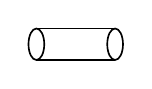
\begin{tikzpicture}[semithick, scale=0.5, baseline=-0.5ex] \begin{scope} \draw (-1,0) ellipse (0.2cm and 0.4cm); \draw (-1,0.4) -- (1,0.4); \draw (-1,-0.4) -- (1,-0.4); \draw (1,0) ellipse (0.2cm and 0.4cm); \end{scope} \end{tikzpicture}
        \quad
        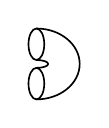
\begin{tikzpicture}[semithick, scale=0.5, baseline=-0.5ex] \begin{scope} \draw (0,0.5) ellipse (0.2cm and 0.4cm); \draw (0,-0.5) ellipse (0.2cm and 0.4cm); \draw (0,0.9) arc (90:-90:1.1cm and 0.9cm); \draw (0,0.1) arc (90:-90:0.3cm and 0.1cm); \end{scope} \end{tikzpicture}
        \quad
        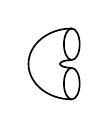
\begin{tikzpicture}[semithick, scale=0.5, baseline=-0.5ex] \begin{scope} \draw (0,0.5) ellipse (0.2cm and 0.4cm);\draw (0,-0.5) ellipse (0.2cm and 0.4cm); \draw (0,0.9) arc (90:270:1.1cm and 0.9cm); \draw (0,0.1) arc (90:270:0.3cm and 0.1cm); \end{scope} \end{tikzpicture}
        \quad
        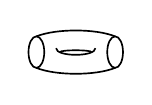
\begin{tikzpicture}[semithick, scale=0.5, baseline=-0.5ex] \begin{scope} \draw (-1,0) ellipse (0.2cm and 0.4cm); \draw (-1,0.4) .. controls (-0.5,0.6) and (0.5,0.6) .. (1,0.4); \draw (-1,-0.4) .. controls (-0.5,-0.6) and (0.5,-0.6) .. (1,-0.4); \draw (-0.5,0.1) .. controls (-0.5,-0.125) and (0.5,-0.125) .. (0.5,0.1); \draw (-0.4,0.0) .. controls (-0.4,0.0625) and (0.4,0.0625) .. (0.4,0.0); \draw (1,0) ellipse (0.2cm and 0.4cm); \end{scope} \end{tikzpicture}
        \quad
        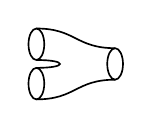
\begin{tikzpicture}[semithick, scale=0.5, baseline=-0.5ex] \begin{scope} \draw (-1,0.5) ellipse (0.2cm and 0.4cm); \draw (-1,-0.5) ellipse (0.2cm and 0.4cm); \draw (1,0) ellipse (0.2cm and 0.4cm); \draw (-1,0.9) .. controls (0,0.9) and (0,0.4) .. (1,0.4); \draw (-1,-0.9) .. controls (0,-0.9) and (0,-0.4) .. (1,-0.4); \draw (-1,0.1) .. controls (-0.2,0.1) and (-0.2,-0.1) .. (-1,-0.1); \end{scope} \end{tikzpicture}
        \quad
        
\begin{tikzpicture}[semithick, scale=0.5, baseline=-0.5ex] \begin{scope} \draw (-1,0) ellipse (0.2cm and 0.4cm); \draw (1,0.5) ellipse (0.2cm and 0.4cm); \draw (1,-0.5) ellipse (0.2cm and 0.4cm); \draw (-1,0.4) .. controls (0,0.4) and (0,0.9) .. (1,0.9); \draw (-1,-0.4) .. controls (0,-0.4) and (0,-0.9) .. (1,-0.9); \draw (1,0.1) .. controls (0.2,0.1) and (0.2,-0.1) .. (1,-0.1); \end{scope} \end{tikzpicture}
        \quad
        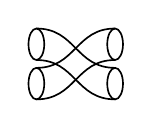
\begin{tikzpicture}[semithick, scale=0.5, baseline=-0.5ex] \begin{scope} \draw (-1,0.5) ellipse (0.2cm and 0.4cm); \draw (-1,-0.5) ellipse (0.2cm and 0.4cm); \draw (1,0.5) ellipse (0.2cm and 0.4cm); \draw (1,-0.5) ellipse (0.2cm and 0.4cm); \draw (-1,0.9) .. controls (0,0.9) and (0,-0.1) .. (1,-0.1); \draw (-1,0.1) .. controls (0,0.1) and (0,-0.9) .. (1,-0.9); \draw (-1,-0.9) .. controls (0,-0.9) and (0,0.1) .. (1,0.1); \draw (-1,-0.1) .. controls (0,-0.1) and (0,0.9) .. (1,0.9); \end{scope} \end{tikzpicture} \]
\end{example}

\begin{example}{bordism}
    Given bordisms $W : M \to M'$ and $W' : M' \to M''$, it can be shown that $W \sqcup_{M'} W'$ admits a smooth structure such that the inclusions $W \to W \sqcup_{M'} W'$ and $W' \to W \sqcup_{M'} W'$ are diffeomorphisms onto their images, which is unique up to (non-unique) diffeomorphism. Hence $W$ and $W'$ can be `composed' to produce a bordism $W' \circ W : M \to M''$, which is well-defined up to isomorphism.
    
    Using this composition rule, one can define the \textit{category of $n$-bordisms} $\textbf{Bord}_n$, where the objects are $(n - 1)$-dimensional closed manifolds and where the morphisms are bordsims are taken up to isomorphism. In particular, the identity morphism of an object $M$ is the cylinder $\id_M = M \times [0, 1]$.
\end{example}

\begin{topic}{lie-algebroid}{Lie algebroid}
    Let $M$ be a \tref{smooth-manifold}{smooth manifold}. A \textbf{Lie algebroid} over $M$ is a \tref{vector-bundle}{vector bundle} $L$ on $M$ together with a \tref{AA:lie-algebra}{Lie bracket} $[\cdot, \cdot]$ on its global sections $\Gamma(L)$ and a map of vector bundles $a : L \to TM$, called the \textit{anchor map}, to the \tref{tangent-bundle}{tangent bundle} of $M$, satisfying
    \begin{itemize}
        \item (\textit{Lie algebra homomorphism}) $a([X, Y]) = [a(X), a(Y)]$ for all $X, Y \in \Gamma(L)$,
        \item (\textit{Leibniz rule}) $[X, fY] = f[X, Y] + (a(X)  f) Y$ for all $X, Y \in \Gamma(L)$ and $f \in C^\infty(M)$.
    \end{itemize}
\end{topic}

\begin{example}{lie-algebroid}
    The tangent bundle $TM$ itself is a Lie algebroid, with the anchor map the identity $\id : TM \to TM$, and Lie bracket the \tref{lie-bracket-vector-fields}{Lie bracket for vector fields}.
\end{example}

\begin{example}{lie-algebroid}
    Given a vector bundle $E \to M$, its \textit{general linear algebroid} is the vector bundle $\mathfrak{gl}(E) \to M$ whose sections are derivations $D : \Gamma(E) \to \Gamma(E)$ of $E$ admitting a vector field $X_D \in TM$ such that $D(f s) = f D(s) + (X_D f) s$ for all $s \in \Gamma(E)$ and $f \in C^\infty(M)$. The Lie bracket is the commutator of differential operators, and the anchor map is the map $D \mapsto X_D$.
\end{example}

\begin{topic}{foliation}{foliation}
    Let $M$ be an $n$-dimensional \tref{smooth-manifold}{smooth manifold}. A $p$-dimensional \textbf{foliation} of $M$ is a decomposition of $M$ into a union of disjoint connected submanifolds
    \[ M = \bigsqcup_{\alpha \in A} L_\alpha \]
    such that each point $x \in M$ has a neighborhood $U$ with local coordinates $x^1, \ldots, x^n$ such that $x^{p + 1}, \ldots, x^n$ are constant on $U \cap L_\alpha$ for all $\alpha \in A$. The submanifolds $L_\alpha$ are called the \textbf{leaves} of the foliation, and the foliation is denoted as $\mathcal{F} = \{ L_\alpha \}_{\alpha \in A}$.
\end{topic}

\begin{topic}{higgs-bundle}{Higgs bundle}
    Let $M$ be a complex manifold. A \textbf{Higgs bundle} on $M$ is a holomorphic vector bundle $E$ on $M$ together with a section $\phi \in \Omega^1(M; \text{End}(E))$, called the \textbf{Higgs field}, satisfying $\phi \wedge \phi = 0$.
\end{topic}

\begin{topic}{frame-bundle}{(tangent) frame bundle}
    The \textbf{frame bundle} of a \tref{vector-bundle}{vector bundle} $E \to M$ of rank $k$ is the vector bundle $F(E) \to M$ whose fibers $F_x$ at a point $x \in M$ is the vector space of ordered bases $\{ e_1, \ldots, e_k \}$ of $E_x$.
    
    There is a natural fiber-wise action of $\text{GL}_k(\RR)$ on $F(E)$ given by change of basis: $\{ e_1, \ldots, e_k \} \cdot g = \{ f_1, \ldots, f_k \}$ where $f_i = \sum_j e_j g_{ji}$. This makes $F(E)$ into a \tref{TO:principal-bundle}{$\text{GL}_k(\RR)$-principal bundle}.
    
    When $E = TM$, the \tref{tangent-bundle}{tangent bundle}, the frame bundle $F(TM)$ is called the \textbf{tangent frame bundle}.
\end{topic}

\begin{topic}{spin-structure}{spin structure}
    Let $(M, g)$ be an $n$-dimensional orientable \tref{riemannian-manifold}{Riemannian manifold}. A \textbf{spin structure} on $M$ is a \tref{TO:principal-bundle}{principal $\text{Spin}(n)$-bundle} $P \to M$ together with a bundle morphism $f : P \to F_{\text{SO}(n)}(M)$ to the oriented orthonormal \tref{frame-bundle}{tangent frame bundle}, equivariant with respect to the double cover $\text{Spin}(n) \to \text{SO}(n)$.
    % Can be generalized to any vector bundle
\end{topic}

\begin{topic}{first-stiefel-whitney-class}{first Stiefel--Whitney class}
    Let $M$ be a \tref{smooth-manifold}{smooth manifold}. There exists a bijection between real line bundles $E \to M$ which can be trivialized over an open cover $\mathcal{U}$ and $\check{H}^1(M, C^\infty(M, \RR^*); \mathcal{U})$, in terms of the transition functions. The group isomorphism
    \[ C^\infty(M, \RR) \times \ZZ_2 \to C^\infty(M, \RR^*), \quad (f, \varepsilon) \mapsto \varepsilon e^f \]
    yields an isomorphism of \tref{AG:cech-cohomology}{Čech cohomology} groups
    \[ \check{H}^k(M; C^\infty(M, \RR); \mathcal{U}) \times \check{H}^k(M; \ZZ_2; \mathcal{U}) \to \check{H}^k(M; C^\infty(M, \RR^*); \mathcal{U}) , \]
    which for $k > 0$ specializes to an isomorphism
    \[ \check{H}^k(M; \ZZ_2; \mathcal{U}) \xrightarrow{\sim} \check{H}^k(M; C^\infty(M, \RR^*); \mathcal{U}) . \]
    The \textbf{first Stiefel--Whitney class} of a real line bundle $E \to M$ is its corresponding class $w_1(E) \in \check{H}^1(M; \ZZ_2; \mathcal{U})$.
    
    The \textbf{first Stiefel--Whitney class} of a rank $k$ real vector bundle $E \to M$ is the first Stiefel--Whitney class of $\wedge^k E$.
\end{topic}

\begin{topic}{first-chern-class}{first Chern class}
    Let $M$ be a \tref{smooth-manifold}{smooth manifold}. There exists a bijection between complex line bundles $E \to M$ which can be trivialized over an open cover $\mathcal{U}$ and $\check{H}^1(M, C^\infty(M, \CC^*); \mathcal{U})$, in terms of the transition functions. The exponential sequence
    \[ 0 \to \ZZ \xrightarrow{2 \pi i} C^\infty(M, \CC) \xrightarrow{\exp} C^\infty(M, \CC^*) \to 0 \]
    yields a long exact sequence of \tref{AG:cech-cohomology}{Čech cohomology} groups
    \[ \cdots \to \check{H}^k(M; \ZZ; \mathcal{U}) \to \check{H}^k(M; C^\infty(M, \CC); \mathcal{U}) \to \check{H}^k(M; C^\infty(M, \CC^*); \mathcal{U}) \to \check{H}^{k + 1}(M; \ZZ; \mathcal{U}) \to \cdots \]
    which in particular gives an isomorphism
    \[ \check{H}^1(M; C^\infty(M, \CC^*); \mathcal{U}) \xrightarrow{\sim} \check{H}^2(M; C^\infty(M, \ZZ; \mathcal{U}) . \]
    The \textbf{first Chern class} of a complex line bundle $E \to M$ is its corresponding class $c_1(E) \in \check{H}^2(M; \ZZ; \mathcal{U})$.
    
    The \textbf{first Chern class} of a rank $k$ complex vector bundle $E \to M$ is the first Chern class of $\wedge^k E$.
\end{topic}

\begin{topic}{determinant-bundle}{determinant bundle}
    The \textbf{determinant bundle} of a \tref{vector-bundle}{vector bundle} $E \to M$ of rank $k$ is the exterior power $\det(E) = \wedge^k E$.
\end{topic}

\begin{topic}{riemann-surface}{Riemann surface}
    A \textbf{Riemann surface} is a \tref{TO:connected-space}{connected} complex manifold of complex dimension one.
\end{topic}

\begin{topic}{volume-form}{volume form}
    Let $M$ be an $n$-dimensional \tref{smooth-manifold}{smooth manifold}. A \textbf{volume form} on $M$ is an \tref{differential-form}{$n$-form} $\omega \in \Omega^n(M)$.
\end{topic}

\begin{example}{volume-form}
    When $M$ is a \tref{riemannian-manifold}{Riemannian manifold} with metric $g$, there is a natural volume form on $M$. In local coordinates $x_1, \ldots, x_n$ it is given by
    \[ \text{vol}_g = \sqrt{|\det g|} \; dx_1 \wedge dx_2 \wedge \cdots \wedge dx_n , \]
    which is indeed independent of the choice of local coordinates.
\end{example}

\begin{topic}{hodge-star-operator}{Hodge star operator}
    Let $(M, g)$ be an $n$-dimensional \tref{riemannian-manifold}{Riemannian manifold}. The \textbf{Hodge star operators} are the maps
    \[ \star : \Omega^k(M) \to \Omega^{n - k}(M) \]
    for $0 \le k \le n$ defined by
    \[ \alpha \wedge \star \beta = g(\alpha, \beta) \text{vol}_g \]
    for all $\alpha, \beta \in \Omega^k(M)$, where $\text{vol}_g = \sqrt{|\det g|} \; dx_1 \wedge \cdots dx_n$ is the \tref{volume-form}{volume form} induced by $g$. Here $g$ is defined on $\Omega^k(M)$ by
    \[ g(\alpha, \beta) = \det\left(g(\alpha_i, \beta_j)\right)_{i, j = 1}^{k} \]
    for decomposable $\alpha = \alpha_1 \wedge \cdots \wedge \alpha_k$ and $\beta = \beta_1 \wedge \cdots \wedge \beta_k$ and extended linearly.
\end{topic}

\begin{topic}{hodge-inner-product}{Hodge inner product}
    Let $(M, g)$ be a \tref{riemannian-manifold}{Riemannian manifold}. The \textbf{Hodge inner product} is the (global) inner product on the de Rham spaces $\Omega^k(M)$ given by
    \[ (\alpha, \beta) = \int_X \alpha \wedge \star \beta = \int_X g(\alpha, \beta) \; \text{vol}_g \]
    for $\alpha, \beta \in \Omega^k(M)$, where $\star$ denotes the \tref{hodge-star-operator}{Hodge star operator}.
\end{topic}

\begin{topic}{de-rham-complex}{de Rham complex}
    Let $M$ be a \tref{smooth-manifold}{smooth manifold}. The \textbf{de Rham complex} of $M$ is the \tref{HA:chain-complex}{cochain complex}
    \[ 0 \to \Omega^0(M) \xrightarrow{d} \Omega^1(M) \xrightarrow{d} \Omega^2(M) \xrightarrow{d} \cdots \]
    where $\Omega^k(M)$ denotes the space of \tref{differential-form}{differential $k$-forms}, and $d$ the \tref{exterior-derivative}{exterior derivative}.
    
    The \textbf{de Rham cohomology groups} $H_\text{dR}^k(M)$ are the \tref{AT:homology-group}{cohomology groups} of $\Omega^\bdot(M)$.
\end{topic}

\begin{topic}{harmonic-form}{harmonic form}
    Let $(M, g)$ be an $n$-dimensional \tref{riemannian-manifold}{Riemannian manifold}. The \tref{exterior-derivative}{exterior derivative} $d : \Omega^k(M) \to \Omega^{k + 1}(M)$ has an adjoint $\delta = (-1)^{nk + 1} \star d \star : \Omega^k(M) \to \Omega^{k - 1}(M)$ with respect to the \tref{hodge-inner-product}{Hodge inner product}. That is,
    \[ (d \alpha, \beta) = (\alpha, \delta \beta) \quad \text{for all } \alpha \in \Omega^k(M) \text{ and } \beta \in \Omega^{k + 1}(M) . \]
    A differential form $\alpha \in \Omega^k(M)$ is \textbf{harmonic} if $\Delta \alpha = 0$, where $\Delta = d \delta + \delta d$ is the \textit{Laplacian operator}.
\end{topic}

\begin{topic}{holonomy-group}{holonomy group}
    Let $\pi : E \to M$ be a \tref{vector-bundle}{vector bundle} over a \tref{smooth-manifold}{smooth manifold} $M$, and $\nabla$ a \tref{connection}{connection} on $E$. By \tref{parallel-transport}{parallel transport}, any loop $\gamma : [0, 1] \to M$ based at a point $x \in M$ yields a linear invertible map $P_\gamma : E_x \to E_x$. The \textbf{holonomy group} of $\nabla$ based at $x$ is the group
    \[ \text{Hol}_x(\nabla) = \{ P_\gamma \in \text{GL}(E_x) : \gamma \text{ is a loop based at } x \} . \]
    The \textbf{restricted holonomy group} is the subgroup $\text{Hol}_x^0(\nabla)$ coming from contractible loops.
\end{topic}

\begin{topic}{implicit-function-theorem}{implicit function theorem}
    The \textbf{implicit function theorem} states that if $f : \RR^{n + m} \to \RR^m$ is a continuously differentiable function, and $p \in \RR^{n + m}$ a point with $f(p) = 0$ such that the Jacobian matrix $J_f = \left(\frac{\partial f_i}{\partial x_j}\right)_{i,j = n + 1}^{n + m}$ is invertible at $p$, then there exists an open set $U \subset \RR^n$ containing $(p_1, \ldots, p_n)$ and a continuously differentiable function $g : U \to \RR^m$ such that $g(p_1, \ldots, p_n) = (p_{n + 1}, \ldots, p_{m + n})$ and $f(y, g(y)) = 0$ for all $y \in U$.
\end{topic}

\begin{topic}{killing-vector-field}{Killing vector field}
    Let $(M, g)$ be a \tref{riemannian-manifold}{Riemannian manifold}. A \tref{vector-field}{vector field} $X$ on $M$ is a \textbf{Killing vector field} if it preserves the metric, i.e. $\mathcal{L}_X g = 0$, where $\mathcal{L}_X$ is the \tref{lie-derivative}{Lie derivative} with respect to $X$.
\end{topic}

\begin{topic}{schouten-nijenhuis-bracket}{Schouten--Nijenhuis bracket}
    The \textbf{Schouten--Nijenhuis bracket} is a unique extension of the \tref{lie-bracket-vector-fields}{Lie bracket of vector fields} to a graded bracket of multivector fields. It is defined by
    \[ \begin{aligned} {[}X_1 \wedge \cdots \wedge X_m, Y_1 \wedge \cdots \wedge Y_n{]} = \sum_{\substack{1 \le i \le m \\ 1 \le j \le n}} (-1)^{i + j} [X_i, X_j] &X_1 \wedge \cdots \wedge X_{i - 1} \wedge X_{i + 1} \wedge X_m \\ \wedge &Y_1 \wedge \cdots \wedge Y_{j - 1} \wedge Y_{j + 1} \wedge Y_n , \end{aligned} \]
    for \tref{vector-field}{vector fields} $X_i$ and $Y_j$, and by
    \[ [f, X_1 \wedge \cdots \wedge X_m] = -\iota_{df} X_1 \wedge \cdots \wedge X_m \]
    for a function $f$.
\end{topic}

\begin{topic}{courant-bracket}{Courant bracket}
    Let $M$ be a \tref{smooth-manifold}{smooth manifold}. The \textbf{Courant bracket} on $M$ is the skew-symmetric bracket on $TM \oplus T^*M$ given by
    \[ [X + \xi, Y + \eta] = [X, Y] + \mathcal{L}_X \eta - \mathcal{L}_Y \xi - \frac{1}{2} d \left(\iota_X \eta - \iota_Y \xi \right) , \]
    where $[X, Y]$ is the usual \tref{lie-bracket-vector-fields}{Lie bracket of vector fields}.
\end{topic}

\begin{topic}{courant-algebroid}{Courant algebroid}
    Let $M$ be a \tref{smooth-manifold}{smooth manifold}. A \textbf{Courant algebroid} over $M$ is a \tref{vector-bundle}{vector bundle} $E$ on $M$ together with a non-degenerate symmetric bilinear form $\langle \cdot, \cdot \rangle : \Gamma(E) \times \Gamma(E) \to \RR$, a skew-symmetric bracket $[\cdot, \cdot] : \Gamma(E) \times \Gamma(E) \to \Gamma(E)$ and a smooth bundle map $\pi : E \to TM$ called the \textit{anchor map}, satisfying
    \begin{itemize}
        \item (\textit{Respecting bracket}) $\pi([X, Y]) = [\pi(X), \pi(Y)]$,
        \item (\textit{Left Jacobi identity}) $[X, [Y, Z]] = [[X, Y], Z] + [Y, [X, Z]]$,
        \item (\textit{Leibniz rule}) $[X, fY] = f[X, X] + \rho(X)(f) Y$,
        \item (\textit{Self-adjoint}) $\pi(X) \langle Y, Z \rangle = \langle [X, Y], Z \rangle + \langle Y, [X, Z] \rangle$,
        \item (\textit{}) $[X, X] = \frac{1}{2} \mathcal{D} \langle X, X \rangle$,
    \end{itemize}
    where $\mathcal{D} : C^\infty(M) \to \Gamma(E)$ is the differential operator.
\end{topic}

\begin{example}{courant-algebroid}
    The bundle $E = TM \oplus T^*M$ together with the bilinear form
    \[ \langle X + \xi, Y + \eta \rangle = \xi(Y) + \eta(X) , \]
    the \tref{courant-bracket}{Courant bracket}, and the projection map $\pi : TM \oplus T^*M \to TM$ as anchor map, is a Courant algebroid, called the \textit{split Courant algebroid}.
\end{example}

\begin{topic}{dirac-structure}{Dirac structure}
    Let $M$ be a \tref{smooth-manifold}{smooth manifold}. An \textbf{almost Diract structure} on $M$ is a subbundle $L \subset TM \oplus T^*M$ which is maximal isotropic with respect to symmetric bilinear form $\langle X + \xi, Y + \eta \rangle = \xi(Y) + \eta(X)$. If moreover $L$ is closed under the \tref{courant-bracket}{Courant bracket}, it is called \textit{integrable}, or simply a \textbf{Dirac structure}.
\end{topic}

% \begin{example}{dirac-structure}

% \end{example}

\begin{topic}{related-vector-fields}{related vector fields}
    Let $f : M \to N$ be a \tref{smooth-map}{smooth map} between \tref{smooth-manifold}{smooth manifolds}. Then vector fields $X$ on $M$ and $Y$ on $M$ are \textbf{$f$-related} if $Y_{f(x)} = (df)_x(X_x)$ for all $x \in M$.
\end{topic}

\begin{topic}{multivector-field}{multivector field}
    Let $M$ be a \tref{smooth-manifold}{smooth manifold}. A \textbf{multivector field} on $M$ is a section of the exterior algebra $\bigwedge^\bdot TM$.
\end{topic}

\begin{topic}{chern-class}{Chern class}
    Let $\pi : E \to M$ be a \tref{vector-bundle}{vector bundle} of rank $n$, and $\nabla$ a \tref{connection}{connection} on $E$ with \tref{curvature-connection}{curvature} $F_\nabla \in \Omega^2(M; \textup{End}(E))$. The \textbf{total Chern form} of $E$ is given by
    \[ C(E) = 1 + c_1(E) + \cdots + c_n(E) = \det \left(1 + \frac{F_\nabla}{2 \pi i} \right) , \]
    where $c_k(E) \in \Omega^{2k}(M)$ is the \textbf{$k$-th Chern form}. The Chern forms are \tref{closed-form}{closed}, and the cohomology class $[c_k(E)] \in H_\textup{dR}^{2k}(M)$ is called the \textbf{$k$-th Chern class} of $E$. These classes are independent on the choice of connection.
\end{topic}

\begin{topic}{chern-character}{Chern character}
    Let $\pi : E \to M$ be a \tref{vector-bundle}{vector bundle}, and $\nabla$ a \tref{connection}{connection} on $E$ with \tref{curvature-connection}{curvature} $F_\nabla \in \Omega^2(M; \textup{End}(E))$. The \textbf{Chern character} of $E$ is given by
    \[ \textup{ch}(E) = \operatorname{tr} \exp \left(\frac{F_\nabla}{2 \pi i} \right) = \sum_{k = 0}^{\infty} \frac{1}{k!} \operatorname{tr} \left(\frac{F_\nabla}{2 \pi i}\right)^k . \]
    The cohomology class $[\textup{ch}(E)] \in H_\textup{dR}^\bdot(M)$ is independent on the choice of connection.
    
    The Chern character satisfies
    \[ [\textup{ch}(E \oplus F)] = [\textup{ch}(E)] + [\textup{ch}(F) ] \quad \text{ and } \quad [\textup{ch}(E \otimes F)] = [\textup{ch}(E)] \cdot [\textup{ch}(F)] . \]
\end{topic}

\begin{topic}{flow-box-theorem}{flow box theorem}
    Let $M$ be a \tref{smooth-manifold}{smooth manifold} with a point $p \in M$, and $X$ a \tref{vector-field}{vector field} such that $X(p) \ne 0$. Then the \textbf{flow box theorem} states that there exist local coordinates $x^1, \ldots, x^n$ around $p$ such that $X = \frac{\partial}{\partial x^1}$.
    
    More generally, if $X_1, \ldots, X_k$ are pairwise commuting vector fields, that is $[X_i, X_j] = 0$ for all $i, j$, which are linearly independent at $p$, then there exist local coordinates $x^1, \ldots, x^n$ such that $X_i = \frac{\partial}{\partial x^i}$.
\end{topic}

\begin{topic}{dolbeault-operators}{Dolbeault operators}
    Let $M$ be a complex manifold. The space $\Omega^{p, q}(M)$ of $(p, q)$-forms is defined by
    \[ \Omega_X^{p, q} = \underbrace{\Omega^{1,0}(M) \wedge \cdots \wedge \Omega^{1,0}(M)}_{\text{$p$ times}} \;\; \wedge \;\; \underbrace{\Omega^{0,1}(M) \wedge \cdots \wedge \Omega^{0,1}(M)}_{\text{$q$ times}} , \]
    where
    \[ \Omega^{1,0}(M) = \left\{ \textstyle\sum_{i = 1}^{n} f_i dz^i \right\} \quad \textup{and} \quad \Omega^{0,1}(M) = \left\{ \textstyle\sum_{i = 1}^{n} g_i d \overline{z}^i \right\} , \]
    and where $z^1, \ldots, z^n$ are local coordinates. Note that these definitions are independent of the chosen coordinates. The \textbf{Dolbeault operators} are the operators
    \[ \partial : \Omega^{p, q}(M) \to \Omega^{p + 1, q}(M) \quad \textup{and} \quad \overline{\partial} : \Omega^{p, q}(M) \to \Omega^{p, q + 1}(M) \]
    given by
    \[ \partial = \sum_{j = 1}^{n} dz^j \wedge \frac{\partial}{\partial z^j} \quad \text{and} \quad \bar{\partial} = \sum_{j = 1}^{n} d\bar{z}^j \wedge \frac{\partial}{\partial \bar{z}^j} . \]
    They satisfy the properties
    \[ \partial + \bar{\partial} = d, \quad \partial^2 = \bar{\partial}^2 = \partial \bar{\partial} + \bar{\partial} \partial = 0 , \]
    where $d$ is the \tref{exterior-derivative}{exterior derivative}.
\end{topic}

\begin{topic}{poincare-lemma}{Poincaré lemma}
    The \textbf{Poincaré lemma} states that on a \tref{AT:contractible-space}{contractible} \tref{smooth-manifold}{smooth manifold} $M$, every \tref{closed-form}{closed $k$-form} is \tref{exact-form}{exact} for $k \ge 1$. In particular, the \tref{de-rham-complex}{de Rham cohomology groups} $H^k_\textup{dR}(M) = 0$ for all $k \ge 1$.
\end{topic}

\begin{topic}{serre-swan-theorem}{Serre--Swan theorem}
    Let $M$ be a \tref{TO:compact-space}{compact} \tref{smooth-manifold}{smooth manifold}. The \textbf{Serre--Swan theorem} states that for any \tref{vector-bundle}{vector bundle} $E \to M$, its global sections $\Gamma(E)$ are a \tref{CA:finitely-generated-module}{finitely generated} \tref{CA:projective-module}{projective} $C^\infty(M)$-module, and conversely that all such modules arise in this way.
    
    In fact, the \tref{CT:functor}{functor} $\Gamma$ yields an \tref{CT:equivalence-of-categories}{equivalence of categories} between the category of vector bundles over $M$ and the category of finitely generated projective $C^\infty(M)$-modules.
\end{topic}

\begin{topic}{todd-class}{Todd class}
    Let $\pi : E \to M$ be a \tref{vector-bundle}{vector bundle}, and $\nabla$ a \tref{connection}{connection} on $E$ with \tref{curvature-connection}{curvature} $F_\nabla \in \Omega^2(M; \textup{End}(E))$. The form
    \[ \det\left(\frac{F_\nabla / 2 \pi i}{\exp(F_\nabla / 2 \pi i) - 1}\right) \in \Omega^\bdot(M) \]
    is \tref{closed-form}{closed}, and its cohomology class $\textup{td}(E) \in H^\bdot_\textup{dR}(M)$, called the \textbf{Todd class} of $E$, is independent of the choice of connection.
    
    The Todd class is multiplicative in the sense that $\textup{td}(E \oplus F) = \textup{td}(E) \cdot \textup{td}(F)$.
\end{topic}

\begin{topic}{dolbeault-cohomology}{Dolbeault cohomology}
    Let $M$ be a complex smooth manifold, and consider the \tref{dolbeault-operators}{Dolbeault operator}
    \[ \overline{\partial} : \Omega^{p, q}(M) \to \Omega^{p, q + 1}(M) . \]
    Since $\overline{\partial}^2 = 0$, one can form the \tref{HA:chain-complex}{complex} $(\Omega^{p, \bdot}(M), \overline{\partial})$, and the corresponding \tref{HA:homology-object}{cohomology group} $H^{p, q}(M, \CC)$ is called the \textbf{$(p, q)$-th Dolbeault cohomology group}.
\end{topic}

\begin{topic}{frobenius-theorem}{Frobeniuw theorem}
    Let $M$ be a \tref{smooth-manifold}{smooth manifold}. \textbf{Frobenius theorem} states there is a one-to-one correspondence between \tref{foliation}{foliations} on $M$ and \tref{involutive-distribution}{involutive distributions} $\mathcal{D} \subset TM$. In particular, a foliation $\mathcal{F}$ corresponds to the involutive distribution $\mathcal{D} = T \mathcal{F}$, where $T_x \mathcal{F} = T_x L$ for any $x \in M$ with $L$ the leaf through $x$.
\end{topic}

\begin{topic}{legendre-transform}{Legendre transform}
    Let $V$ be a real \tref{LA:vector-space}{vector space} and $f : V \to \RR$ a smooth function which is \textit{super-linear}, that is, $\sup_{v \in V} \left(p(v) - f(v) \right) < \infty$ for all $p \in V^*$. Then the \textbf{Legendre transform} of $f$ is
    \[ f^* : V^* \to \RR, \quad p \mapsto \sup_{v \in V} \left(p(v) - f(v) \right) . \]
\end{topic}

\begin{example}{legendre-transform}
    Let $Q$ be a \tref{smooth-manifold}{smooth manifold} and $L \in C^\infty(TM)$ a smooth function on the \tref{tangent-bundle}{tangent bundle}. Assume $L$ is fiberwise super-linear, i.e. $L(q, -) : T_q M \to \RR$ is super-linear for all $q \in Q$. Then the Legendre transform of $L$ is
    \[ H : T^*M \to \RR, \qquad (q, p) \mapsto \left(L(q, -)\right)^*(p) . \]
    In physics, in particular classical mechanics, $L$ is the \textit{Lagrangian} for a mechanical system with configuration space $Q$, and the Legendre transform $H = L^*$ is the \textit{Hamiltonian} of the system.
\end{example}

\begin{example}{legendre-transform}
    Let $f : V \to \RR$ be given by $f(v) = \tfrac{1}{2} g(v, v)$, for some positive definite metric $g : V \times V \to \RR$. Given some fixed $p \in V^*$, we can find the supremum $\sup_{v \in V} \left(p(v) - \tfrac{1}{2} g(v, v)\right)$ by looking for extreme values. Setting
    \[ \partial_k \left( p_i v^i - \frac{1}{2} g_{ij} v^i v^j \right) = p_k - g_{ki} v^i \]
    equal to zero gives $v^i = g^{ik} p_k$, and thus
    \[ f^*(p) = p_i g^{ik} p_k - \frac{1}{2} g_{ij} g^{i k} p_k g^{j \ell} p_\ell = \frac{1}{2} g^{ik} p_i p_k , \]
    that is, $f^*(p) = g^*(p, p)$ where $g^* : V^* \times V^* \to \RR$ is the dual metric.
\end{example}

\begin{topic}{symplectic-manifold}{symplectic manifold}
    Let $M$ be a \tref{smooth-manifold}{smooth manifold}. A \textbf{symplectic form} on $M$ is a \tref{closed-form}{closed} and non-degenerate \tref{differential-form}{$2$-form} $\omega$ on $M$. The pair $(M, \omega)$ is called a \textbf{symplectic manifold}.
\end{topic}

\begin{example}{symplectic-manifold}
    Let $M = \RR^{2n}$ with standard coordinates $q^1, \ldots, q^n, p_1, \ldots, p_n$. Then the $2$-form
    \[ \omega = \sum_{i = 1}^{n} d q^i \wedge d p_i , \]
    is a symplectic form, the \textit{standard symplectic form}.
    
    In fact, \tref{darboux-theorem}{Darboux's theorem} states that any symplectic manifold locally has this form.
\end{example}

\begin{topic}{symplectomorphism}{symplectomorphism}
    A \textbf{symplectomorphism} is a \tref{diffeomorphism}{diffeomorphism} $\varphi : M \to M'$ between \tref{symplectic-manifold}{symplectic manifolds} $(M, \omega)$ and $(M', \omega')$ satisfying $\varphi^* \omega' = \omega$.
\end{topic}

\begin{topic}{tautological-one-form}{tautological 1-form}
    Let $Q$ be a \tref{smooth-manifold}{smooth manifold}. The \textbf{tautological $1$-form} is the \tref{differential-form}{$1$-form} $\theta$ on the \tref{cotangent-bundle}{cotangent bundle} $T^*Q$ given by
    \[ \theta_x = p(d \pi_x) \quad \text{ for all } x = (q, p) \in T^*Q , \]
    where $\pi : T^*Q \to Q$ denotes the projection.
\end{topic}

\begin{example}{tautological-one-form}
    Take $Q = \RR^n$ so that $T^* Q \simeq \RR^{2n}$ with standard coordinates $q^1, p_1, \ldots, q^n, p_n$. Then the tautological $1$-form is given by
    \[ \theta = \sum_{i = 1}^{n} p_i dq^i . \]
\end{example}

\begin{topic}{canonical-symplectic-form}{canonical symplectic form}
    Let $Q$ be a \tref{smooth-manifold}{smooth manifold}. The \textbf{canonical symplectic form} is the \tref{symplectic-manifold}{symplectic form} $\omega$ on the \tref{cotangent-bundle}{cotangent bundle} $T^* Q$ given by
    \[ \omega = -d \theta , \]
    where $\theta$ is the \tref{tautological-one-form}{tautological $1$-form}.
\end{topic}

\begin{example}{canonical-symplectic-form}
    Take $Q = \RR^n$ so that $T^* Q \simeq \RR^{2n}$ with standard coordinates $q^1, p_1, \ldots, q^n, p_n$. Then the tautological $1$-form is given by
    \[ \theta = \sum_{i = 1}^{n} p_i dq^i , \]
    and thus the canonical symplectic form is given by
    \[ \omega = -d \theta = \sum_{i = 1}^{n} d q^i \wedge d p_i. \]
\end{example}

\begin{topic}{symplectic-vector-field}{symplectic vector field}
    Let $(M, \omega)$ be a \tref{symplectic-manifold}{symplectic manifold}. A \tref{vector-field}{vector field} $X$ on $M$ is called \textbf{symplectic} if the \tref{interior-product}{interior product}
    \[ \iota_X \omega = \omega(X, -) \]
    is \tref{closed-form}{closed}.
\end{topic}

\begin{example}{symplectic-vector-field}
    Every \tref{hamiltonian-vector-field}{Hamiltonian vector field} is symplectic, since every exact form is closed. The converse is however not true. Let $M$ be the $2n$-torus $\RR^{2n}/\ZZ^{2n}$ with the standard symplectic form
    \[ \omega = \sum_{i = 1}^{n} dp_i \wedge dq^i . \]
    Then the vector field $X$ on $M$ given by $X(x) = v$ for some constant non-zero $v \in \RR^{2n}$ (identifying $T_x M$ canonically with $\RR^{2n}$) is symplectic, but not Hamiltonian.
\end{example}

\begin{topic}{hamiltonian-vector-field}{Hamiltonian vector field}
    Let $(M, \omega)$ be a \tref{symplectic-manifold}{symplectic manifold}. Every smooth function $H : M \to \RR$ uniquely determines a \tref{vector-field}{vector field} $X_H$ satisfying
    \[ \omega(X_H, -) = dH . \]
    Such a vector field is called a \textbf{Hamiltonian vector field} with \textbf{Hamiltonian $H$}.
\end{topic}

\begin{example}{hamiltonian-vector-field}
    Let $M = \RR^{2n}$ with the standard symplectic form
    \[ \omega = \sum_{i = 1}^{n} dp_i \wedge dq^i . \]
    Then the Hamiltonian vector field with Hamiltonian $H$ has the form
    \[ X_H = \left(\frac{\partial H}{\partial p_i}, -\frac{\partial H}{\partial q^i} \right) . \]
\end{example}

\begin{topic}{symplectic-action}{symplectic action}
    Let $(M, \omega)$ be a \tref{symplectic-manifold}{symplectic manifold} and $G$ a \tref{lie-group}{Lie group} acting on $M$. The action is called \textbf{symplectic} if every element of $G$ acts by a \tref{symplectomorphism}{symplectomorphism}.
\end{topic}

\begin{topic}{fundamental-vector-field}{fundamental vector field}
    Let $M$ be a \tref{smooth-manifold}{smooth manifold}, $G$ a \tref{lie-group}{Lie group} acting on $M$ via $\varphi : G \times M \to M$. For any $\xi \in \mathfrak{g}$ in the Lie algebra of $G$, the \textbf{fundamental vector field} of $\xi$ is the \tref{vector-field}{vector field} on $M$ given by
    \[ X_\xi(p) = d(\varphi(-, p))(e) \xi \in T_p M . \]
    Alternatively, we have
    \[ X_\xi(p) = \frac{d}{d t}\Big|_{t = 0} \varphi(\exp(t \xi), p) . \]
\end{topic}

\begin{topic}{moment-map}{moment map}
    Let $(M, \omega)$ be a \tref{symplectic-manifold}{symplectic manifold} and $G$ a \tref{lie-group}{Lie group} with a \tref{symplectic-action}{symplectic action} on $M$. A \textbf{moment map} for the action is a smooth map $\mu : M \to \mathfrak{g}^*$ such that
    \[ d \langle \mu, \xi \rangle = \omega(X_\xi, -) \]
    for all $\xi \in \mathfrak{g}$, and such that $\mu$ is $G$-equivariant with respect to the \tref{adjoint-representation}{co-adjoint representation} of $G$, that is,
    \[ \mu(g \cdot p) = \text{Ad}_G^* (g) \mu(p) \]
    for all $p \in M$ and $g \in G$.
\end{topic}

\begin{topic}{hamiltonian-manifold}{Hamiltonian manifold}
    Let $(M, \omega)$ be a \tref{symplectic-manifold}{symplectic manifold} and $G$ a \tref{lie-group}{Lie group} with a \tref{symplectic-action}{symplectic action} $\varphi : G \times M \to M$ on $M$. The action is \textbf{Hamiltonian} if it admits a \tref{moment-map}{moment map}.
    
    The collection $(M, \omega, G, \varphi, \mu)$ is called a \textbf{Hamiltonian manifold}.
\end{topic}

\begin{topic}{marsden-weinstein-quotient}{Marsden--Weinstein quotient}
    Let $(M, \omega, G, \varphi, \mu)$ be a \tref{hamiltonian-manifold}{Hamiltonian manifold}, and assume $G$ acts \tref{GT:free-group-action}{freely} and \tref{GT:proper-group-action}{properly} on the zero-level set of the \tref{moment-map}{moment map} $\mu^{-1}(0) \subset M$. The \textbf{Marsden--Weinstein theorem} states that the orbit space
    \[ M \sslash G := \mu^{-1}(0) / G \]
    is a \tref{symplectic-manifold}{symplectic manifold} in a canonical way, called the \textbf{Marsden--Weinstein quotient} of $M$ by $G$. That is, there exists a unique symplectic form $\overline{\omega}$ on $M \sslash G$ which pulls back to the restriction of $\omega$ on $\mu^{-1}(0) / G$.
    
    Furthermore,
    \[ \dim(M \sslash G) = \dim M - 2 \dim G . \]
\end{topic}

\begin{topic}{poisson-manifold}{Poisson manifold}
    Let $M$ be a \tref{smooth-manifold}{smooth manifold}. A \textbf{Poisson structure} on $M$ is a bracket $\{ \cdot, \cdot \}$ on the algebra $C^\infty(M)$ of smooth functions making it into a \tref{AA:poisson-algebra}{Poisson algebra}. A \textbf{Poisson manifold} is a manifold with a Poisson structure.
\end{topic}

\begin{example}{poisson-manifold}
    Any \tref{symplectic-manifold}{symplectic manifold} $(M, \omega)$ gives rise to a Poisson manifold with bracket given by
    \[ \{ F, G \} = \omega(X_F, X_G) \]
    where $X_F$ is the \tref{hamiltonian-vector-field}{Hamiltonian vector field} of $F$.
    Indeed the Leibniz rule is satisfied as
    \[ \{ FG, H \} = d(FG) X_H = (F d G + G d F) X_H = F (d G X_H) + G (d F X_H) = F \{ G, H \} + G \{ F, H \} . \]
    Furthermore, the Jacobi identity can be shown from
    \[ \{ \{ F, G \}, H \} + \{ \{ G, H \}, F \} + \{ \{ H, F \}, G \} = -d \omega(X_F, X_G, X_H) \]
    and that $\omega$ is closed.
\end{example}

\begin{topic}{poisson-map}{Poisson map}
    A \textbf{Poisson map} is a \tref{smooth-map}{smooth map} $\phi : M \to N$ between \tref{poisson-manifold}{Poisson manifolds} such that the pullback
    \[ \phi^* : C^\infty(N) \to C^\infty(M), \quad f \mapsto f \circ \phi \]
    is a morphism of Poisson algebras.
\end{topic}

\begin{topic}{darboux-theorem}{Darboux's theorem}
    Let $(M, \omega)$ be a \tref{symplectic-manifold}{symplectic manifold}. \textbf{Darboux's theorem} states that around any point $x \in M$, there are local coordinates $q^1, \ldots, q^n, p_1, \ldots, p_n$ such that
    \[ \omega = dq^i \wedge dp_i . \]
\end{topic}

\begin{example}{darboux-theorem}
    \textbf{Proof}. Locally around $x$, we can write $\omega = \frac{1}{2} \omega_{ij} dx^i \wedge dx^j$. Consider $\omega_0 = \frac{1}{2} \omega_{ij}(x) dx^i \wedge dx^1$, which is also a symplectic form in the same neighborhood of $x$. Moreover, for a sufficiently small neighborhood around $x$, we have a family of symplectic forms
    \[ \omega(t) = (1 - t) \omega_0 + t \omega , \quad t \in [0, 1] . \]
    Since $\omega - \omega_0$ is closed, using \tref{poincare-lemma}{Poincaré's lemma} we can locally around $x$ write $\dot{\omega}(t) = \omega - \omega_0 = - d \lambda$ for some $1$-form $\lambda$. Since $\omega - \omega_0$ vanishes at $x$, we may choose $\lambda$ to vanish at $x$ up to second order. Now let $X(t)$ be the vector field defined by $\iota_{X(t)} \omega(t) = \lambda$, and let $\varphi_t$ be the flow of $X(t)$ around $x_0$. Since $\varphi_t(x) = x$ for all $t \in [0, 1]$, the flow $\varphi_t$ exists on the whole interval $t \in [0, 1]$ sufficiently close to $x$. Now,
    \[ \frac{d}{dt} \varphi_t^* \omega(t) = \varphi_t^* \left(\frac{\partial \omega(t)}{\partial t} + \mathcal{L}_{X(t)} \omega(t) \right) = \varphi_t^* \left(\frac{\partial \omega(t)}{\partial t} + d(\iota_{X(t)} \omega(t)) \right) = \varphi_t^* \left( -d \lambda + d \lambda \right) = 0 , \]
    using the \tref{cartan-formula}{Cartan formula}. This implies that $\varphi_1^* \omega = \varphi_1^* \omega(1) = \varphi_0^* \omega(0) = \omega_0$, so $\varphi_1$ is the desired diffeomorphism. Finally, by a linear change of variables the form $\omega_0$ can be reduced to the canonical form.
\end{example}

\begin{topic}{moser-stability}{Moser's stability}
    \textbf{Moser's stability} states that for a \tref{closed-manifold}{closed} \tref{smooth-manifold}{smooth manifold} $M$ and a family of \tref{symplectic-manifold}{symplectic forms} $(\omega_t)_{t \in [0, 1]}$ on $M$ such that the \tref{de-rham-complex}{cohomology classes} $[\omega_t] \in H^2_{\textup{dR}}(M)$ are constant, there exists an isotopy $\varphi : M \times [0, 1] \to M$ such that $\varphi_t^* \omega_0 = \omega_t$ for all $t \in [0, 1]$.
\end{topic}

\begin{example}{moser-stability}
    The proof is known as \textbf{Moser's trick}. Suppose there exists such an isotopy $\varphi$, and define a vector field $X_t = \frac{d \varphi}{d t} \circ \varphi_t^{-1}$. Then by \tref{cartan-formula}{Cartan's formula} and properties of the \tref{lie-derivative}{Lie derivative},
    \[ 0 = \frac{d}{dt} \left(\varphi_t^* \omega_t\right) = \varphi_t^* \left(\mathcal{L}_{X_t} \omega_t + \frac{d}{dt} \omega_t \right) = \varphi_t^* \left(d \iota_{X_t} \omega_t + \frac{d}{dt} \omega_t \right) \]
    so we obtain
    \[ d \iota_{X_t} \omega_t + \frac{d \omega_t}{dt} = d(\iota_{X_t} \omega_t + \alpha_t) = 0 , \]
    where $\frac{d \omega_t}{d t} = d \alpha_t$ for a family of 1-forms $\alpha_t$ since $[\omega_t]$ is constant. Now since $\omega_t$ is non-degenerate, we can integrate $\iota_{X_t} \omega_t + \alpha_t$ to obtain $X_t$, and let $\varphi_t$ be the flow of $X_t$.
\end{example}

\begin{topic}{casimir-function}{Casimir function}
    Let $(P, \{ \cdot, \cdot \})$ be a \tref{poisson-manifold}{Poisson manifold}. A function $f \in C^\infty(P)$ is called \textbf{Casimir} if the \tref{hamiltonian-vector-field}{Hamiltonian vector field} $X_f = \{ f, - \}$ is zero.
\end{topic}

\begin{topic}{symplectic-connection}{symplectic connection}
    Let $(M, \omega)$ be a \tref{symplectic-manifold}{symplectic manifold}. A \textbf{symplectic connection} on $M$ is a \tref{affine-connection}{affine connection} $\nabla$ which is \tref{torsion-connection}{torsion-free} and preserves the symplectic form, that is
    \[ (\nabla_Z \omega)(X, Y) = d(w(X, Y)) - \omega(\nabla_Z X, Y) - \omega(X, \nabla_Z Y) = 0 \]
    for any \tref{vector-field}{vector fields} $X, Y$ and $Z$.
\end{topic}

\begin{topic}{fubini-study-form}{Fubini--Study form}
    The \textbf{Fubini--study form} on $\CC \PP^n$ is the unique $2$-form $\omega_\textup{FS}$ on $\CC \PP^n$ such that
    \[ \pi^* \omega_\textup{FS} = \frac{i}{2} \partial \bar{\partial} \log (|\cdot|^2) , \]
    where $\pi : \CC^n \setminus \{ 0 \} \to \CC \PP^n$ is the projection map, $\partial$ and $\bar{\partial}$ are the \tref{dolbeault-operators}{Dolbeault operators}, and $|\cdot| : \CC^n \to \RR$ is the Euclidean norm. It is a \tref{symplectic-manifold}{symplectic form}.
\end{topic}

\begin{topic}{compatible-triple}{compatible triple}
    Let $M$ be a \tref{smooth-manifold}{smooth manifold}. A \textbf{compatible triple} on $M$ is a triple $(\omega, J, g)$, where $\omega$ is a \tref{symplectic-manifold}{symplectic form} on $M$, $J$ is an \tref{complex-manifold}{almost complex structure} on $M$, and $g$ is a \tref{riemannian-manifold}{Riemannian metric} on $M$, such that
    \[ g(X, Y) = \omega(X, J(Y)) \]
    for all \tref{vector-field}{vector fields} $X$ and $Y$ on $M$.
    % Given two out of the three structures of a compatible triple, the third structure can be obtained.
\end{topic}

\begin{example}{compatible-triple}
    Let $M = \CC^n$ with the standard Hermitian metric $h(-, -)$. Decomposing in real and imaginary parts, we have
    \[ h(u, v) = g(u, v) + i \omega(u, v) \]
    for some bilinear forms $g$ and $\omega$. Since $h(v, u) = \overline{h(u, v)}$, it follows that $g$ is symmetric and $\omega$ is skew-symmetric. Moreover, $g$ and $\omega$ are non-degenerate since $h$ is. In particular, $g$ is a Riemannian metric, and $\omega$ a symplectic form. Furthermore, multiplication by $i$ defines an almost complex structure $J$. Note that
    \[ g(u, Jv) + i \omega(u, Jv) = h(u, iv) = i h(u, v) = i g(u, v) - \omega(u, v) , \]
    from which follows that
    \[ g(u, v) = \omega(u, Jv) , \]
    that is, $(\omega, J, g)$ is a compatible triple.
\end{example}

\begin{topic}{weyl-bundle}{Weyl bundle}
    Let $(M, \omega)$ be a \tref{symplectic-manifold}{symplectic manifold}. The \textbf{Weyl bundle} on $M$ is the \tref{vector-bundle}{vector bundle}
    \[ W = \widehat{\textup{Sym}}(T^*M) , \]
    that is, the \tref{CA:completion}{completed} \tref{CA:symmetric-algebra}{symmetric algebra} of the \tref{cotangent-bundle}{cotangent bundle}.
    
    The \textbf{formal Weyl algebra} is the vector bundle
    \[ W_\hbar = \widehat{\textup{Sym}}(T^*M) \llbracket \hbar \rrbracket , \]
    where $\hbar$ is a formal parameter.
\end{topic}

\begin{topic}{moyal-weyl-product}{Moyal--Weyl product}
    Let $(M, \omega)$ be a \tref{symplectic-manifold}{symplectic manifold}. The \textbf{Moyal--Weyl product} is a non-commutative product on the sections of the \tref{weyl-bundle}{formal Weyl bundle} $W_\hbar$. In local coordinates, if $y^1, \ldots, y^{2n}$ is a basis for $T^*M$, the Moyal--Weyl product is given by
    \[ \begin{aligned}
        a \circ b
            &= \left. \exp \left(-\frac{i\hbar}{2} \omega^{ij} \frac{\partial}{\partial y^i} \frac{\partial}{\partial z^j}\right) a(y) b(z) \right|_{z = y} \\
            &= \sum_{k = 0}^{\infty} \left(-\frac{i\hbar}{2}\right)^k \frac{1}{k!} \omega^{i_1 j_1} \cdots \omega^{i_k j_k} \frac{\partial^k a}{\partial y^{i_1} \cdots \partial y^{i_k}} \frac{\partial^k b}{\partial y^{j_1} \cdots \partial y^{j_k}} ,
    \end{aligned} \]
    for sections $a, b \in \Gamma(W_\hbar)$.
\end{topic}

\begin{example}{moyal-weyl-product}
    The center of $\Gamma(W_\hbar)$ with respect to the Weyl product is $C^\infty(M)\llbracket \hbar \rrbracket$. Namely, if $a$ is in the center of $\Gamma(W_\hbar)$ and $b = y^k$ for some $k$, then
    \[ a \circ b = a y^k - \frac{i\hbar}{2} \omega^{ik} \frac{\partial a}{\partial y^i} \qquad \text{ and } \qquad b \circ a = a y^k - \frac{i\hbar}{2} \omega^{kj} \frac{\partial a}{\partial y^j} , \]
    so
    \[ 0 = a \circ b - b \circ a = - i \hbar \omega^{ik} \frac{\partial a}{\partial y^i} . \]
    Varying $k$, we find that $\frac{\partial a}{\partial y^i} = 0$ for all $i$, so $a \in C^\infty(M)\llbracket \hbar \rrbracket$. The converse inclusion is straightforward.
\end{example}

\begin{topic}{fedosov-manifold}{Fedosov manifold}
    A \textbf{Fedosov manifold} is a triple $(M, \omega, \nabla)$, where $(M, \omega)$ is a \tref{symplectic-manifold}{symplectic manifold} and $\nabla$ is a \tref{torsion-connection}{torsion-free} \tref{symplectic-connection}{symplectic connection} on $M$.
\end{topic}

\begin{example}{fedosov-manifold}
    Any symplectic manifold $(M, \omega)$ admits a torsion-free symplectic connection. Namely, by \tref{darboux-theorem}{Darboux's theorem}, there exists a covering of $M$ by \textit{Darboux charts}, which are open subsets of the standard symplectic space $\RR^{2n}$ with coordinates $q^1, \ldots, q^n, p_1, \ldots, p_n$ and symplectic form $\omega = \sum_{i = 1}^{n} dq^i \wedge dp_i$. On such a standard symplectic space, the \tref{exterior-derivative}{exterior derivative} $d$ is a torsion-free symplectic connection, and gluing these using a \tref{partition-of-unity}{partition of unity}, we obtain a global torsion-free symplectic connection on $M$.
\end{example}

\begin{topic}{lie-group}{Lie group}
    A \textbf{Lie group} is a \tref{GT:group}{group} $G$ which is also a finite-dimensional \tref{smooth-manifold}{smooth manifold}, such that the multiplication map $G \times G \to G : (x, y) \mapsto xy$ and the inversion map $G \to G : x \mapsto x^{-1}$ are \tref{smooth-map}{smooth}.
\end{topic}

\begin{topic}{adjoint-representation}{adjoint representation}
    The \textbf{adjoint representation} of a \tref{lie-group}{Lie group} $G$ is a \tref{RT:representation}{representation} onto its Lie algebra $\mathfrak{g} = T_e G$ given by
    \[ \text{Ad}_G : G \to \text{GL}(\mathfrak{g}), \quad g \mapsto \text{Ad}_g := d c_g(e) , \]
    where $c_g : G \to G, h \mapsto g h g^{-1}$ denotes the \tref{GT:conjugation}{conjugation} map.
    
    The \textbf{co-adjoint representation} $\text{Ad}_G^* : G \to \text{GL}(\mathfrak{g}^*)$ is the \tref{RT:dual-representation}{dual representation} of $\text{Ad}_G$.
    
    The \textbf{adjoint representation} of a \tref{AA:lie-algebra}{Lie algebra} $\mathfrak{g}$ is a representation onto itself, given by
    \[ \text{ad}_{\mathfrak{g}}: \mathfrak{g} \to \mathfrak{gl}(\mathfrak{g}), \quad X \mapsto [X, -] . \]
\end{topic}


\chapter{Algebraic Geometry}
\renewcommand{\cat}{AG}
\begin{topic}{sheaf}{sheaf}
    Let $X$ be a \tref{TO:topological-space}{topological space}. A \textbf{presheaf} $\mathcal{F}$ of abelian groups on $X$ consists of
    \begin{itemize}
        \item an \tref{GT:abelian-group}{abelian group} $\mathcal{F}(U)$ for every open subset $U \subset X$,
        \item a \tref{GT:group-homomorphism}{group morphism} $r_{UV} : \mathcal{F}(U) \to \mathcal{F}(V)$ for every inclusion $V \subset U$ of open subsets of $X$,
    \end{itemize}
    such that
    \begin{itemize}
        \item $r_{UU}$ is the identity map for any open $U \subset X$,
        \item if $W \subset V \subset U$ are open subsets of $X$, then $r_{UW} = r_{VW} \circ r_{UV}$.
    \end{itemize}
    Elements of $\mathcal{F}(U)$ are called \textit{sections}. The maps $r_{UV}$ are thought of as restriction maps, and for this reason $r_{UV}(s)$ is often simply written as $s|_V$, for $s \in \mathcal{F}(V)$. One can similarly define a presheaf of rings, sets, etc.
    
    A presheaf $\mathcal{F}$ is a \textbf{sheaf} if it moreover satisfies:
    \begin{itemize}
        \item for any open $U \subset X$ and open covering $\{ U_i \}$ of $U$, if $s \in \mathcal{F}(U)$ is such that $s|_{U_i} = 0$ for all $i$, then $s = 0$.
        \item for any open $U \subset X$ and open covering $\{ U_i \}$ of $U$, suppose we have elements $s_i \in \mathcal{F}(U_i)$ such that $s_i|{U_i \cap U_j} = s_j|_{U_i \cap U_j}$ for all $i, j$. Then there is an element $s \in \mathcal{F}(U)$ such that $s_i = s|_{U_i}$ for all $i$. (Note that uniqueness follows from the above condition.)
    \end{itemize}
    
    A morphism of presheaves $f : \mathcal{F} \to \mathcal{G}$ consists of a morphism of abelian groups $f(U) : \mathcal{F}(U) \to \mathcal{G}(U)$ for each open set $U$, such that for every inclusion $V \subset U$ the diagram
    \[ \begin{tikzcd} \mathcal{F}(U) \arrow{r}{f(U)} \arrow[swap]{d}{r_{UV}} & \mathcal{G}(U) \arrow{d}{r'_{UV}} \\ \mathcal{F}(V) \arrow{r}{f(V)} & \mathcal{G}(V) \end{tikzcd} \]
    commutes. A morphism of sheaves is a morphism of presheaves.
\end{topic}

\begin{topic}{constant-sheaf}{constant sheaf}
    Let $X$ be a \tref{TO:topological-space}{topological space}, and $A$ an \tref{GT:abelian-group}{abelian group}. The \textbf{constant sheaf} $\underline{A}$ on $X$ determined by $A$ is the \tref{sheaf}{sheaf} given by
    \[ \underline{A}(U) = \{ \textup{locally constant functions } U \to A \} , \]
    and the usual restriction maps. Note that for every \tref{TO:connected-space}{connected} open set $U$ we have $\underline{A}(U) \simeq A$, hence the name `constant sheaf'.
    
    A sheaf $\mathcal{F}$ on $X$ is \textbf{locally constant} if every point has an open neighborhood $U$ such that $\mathcal{F}|_U$ is isomorphic to a \textbf{constant sheaf}.
\end{topic}

\begin{topic}{stalk}{stalk}
    Let $\mathcal{F}$ be a \tref{sheaf}{presheaf} on a topological space $X$, and take a point $x \in X$. The \textbf{stalk} $\mathcal{F}_x$ of $\mathcal{F}$ at $x$ is defined as the direct limit of the groups $\mathcal{F}(U)$ for all open sets $U$ containing $x$, via the restriction maps.
\end{topic}

\begin{topic}{associated-sheaf}{associated sheaf}
    Given a \tref{sheaf}{presheaf} $\mathcal{F}$, there is a \tref{sheaf}{sheaf} $\mathcal{F}^+$ and a morphism $\theta : \mathcal{F} \to \mathcal{F}^+$, with the property that for any sheaf $\mathcal{G}$ and morphism $f : \mathcal{F} \to \mathcal{G}$ there is a unique morphism $g : \mathcal{F}^+ \to \mathcal{G}$ such that $f = g \circ \theta$. The sheaf $\mathcal{F}^+$ is called the \textbf{sheaf associated} to the presheaf $\mathcal{F}$.
    \[ \begin{tikzcd} \mathcal{F} \arrow{rr}{f} \arrow[swap]{dr}{\theta} && \mathcal{G} \\ & \mathcal{F}^+ \arrow[swap,dashed]{ur}{g} & \end{tikzcd} \]
\end{topic}

\begin{topic}{direct-image-sheaf}{direct image sheaf}
    Let $f : X \to Y$ be a map of \tref{TO:topological-space}{topological spaces}, and let $\mathcal{F}$ be a \tref{sheaf}{sheaf} on $X$. The \textbf{direct image sheaf} $f_* \mathcal{F}$ on $Y$ is defined by
    \[ (f_* \mathcal{F})(V) = \mathcal{F}(f^{-1}(V)) \]
    for any open set $V \subset Y$ (indeed this presheaf is a sheaf).
    
    This construction yields the \textbf{direct image functor}
    \[ f_* : \textup{Sh}(X) \to \textup{Sh}(Y) , \]
    which is \tref{CT:adjunction}{right adjoint} to the \tref{inverse-image-sheaf}{inverse image functor} $f^{-1}$.
    
    When $f : X \to Y$ is a morphism of \tref{scheme}{schemes} and $\mathcal{F}$ an \tref{O-module}{$\mathcal{O}_X$-module}, the direct image $f^* \mathcal{F}$ is a $\mathcal{O}_Y$-module, getting its structure via $f^\# : \mathcal{O}_Y \to f_* \mathcal{O}_X$. Again we have a adjunction $f^* \dashv f_*$.
\end{topic}

\begin{topic}{inverse-image-sheaf}{inverse image sheaf}
    Let $f : X \to Y$ be a map of topological spaces, and let $\mathcal{G}$ be a \tref{sheaf}{sheaf} on $Y$. The \textbf{inverse image sheaf} $f^
    {-1}\mathcal{G}$ on $X$ is defined as the \tref{associated-sheaf}{sheaf associated} to the presheaf given by $U \mapsto \lim_{V \supset f(U)} \mathcal{G}(V)$ for any open set $U \subset X$.
    
    This construction yields the \textbf{inverse image functor}
    \[ f^{-1} : \textup{Sh}(Y) \to \textup{Sh}(X) . \]
    It is the \tref{CT:adjunction}{left adjoint} of the \tref{direct-image-sheaf}{direct image functor} $f_* : \textup{Sh}(X) \to \textup{Sh}(Y)$.
    
    When $f : X \to Y$ is a morphism of \tref{scheme}{schemes}, and $\mathcal{G}$ an \tref{O-module}{$\mathcal{O}_Y$-module}, the \textbf{inverse image sheaf} $f^* \mathcal{G}$ is the $\mathcal{O}_X$-module defined by
    \[ f^* \mathcal{G} = f^{-1} \mathcal{G} \otimes_{f^{-1} \mathcal{O}_Y} \mathcal{O}_X . \]
    Again we have an adjunction $f^* \dashv f_*$.
\end{topic}

\begin{topic}{flasque-sheaf}{flasque sheaf}
    A \tref{sheaf}{sheaf} $\mathcal{F}$ on a topological space $X$ is called \textbf{flasque} if for every inclusion $V \subset U$ of open sets, the restriction map $\mathcal{F}(U) \to \mathcal{F}(V)$ is surjective.
\end{topic}

\begin{topic}{skyscraper-sheaf}{skyscraper sheaf}
    Let $X$ be a topological space, $A$ an abelian group, and take a point $x \in X$. The \textbf{skyscraper sheaf} $i_x(A)$ at $x$ with value $A$ is defined as
    \[ i_x(A) (U) = \left\{ \begin{array}{cl} A & \text{if } x \in U, \\ 0 & \text{otherwise.} \end{array} \right. \]
    The stalks of this sheaf are $A$ at any point in the closure of $x$, and zero elsewhere.
    
    Equivalently, it is the \tref{direct-image-sheaf}{direct image sheaf} $i_*(\underline{A})$ for $\underline{A}$ the \tref{constant-sheaf}{constant sheaf} determined by $A$ on the closure $\overline{\{ x \}}$ and $i : \overline{\{ x \}} \to X$ the inclusion.
\end{topic}

\begin{topic}{sheaf-hom}{sheaf hom}
    Let $\mathcal{F}$ and $\mathcal{G}$ be \tref{sheaf}{sheaves} of abelian groups on a topological space $X$. The \textbf{sheaf hom} of $\mathcal{F}$ and $\mathcal{G}$ is the sheaf $\underline{\Hom}(\mathcal{F}, \mathcal{G})$ given by
    \[ \underline{\Hom}(\mathcal{F}, \mathcal{G})(U) = \Hom(\mathcal{F}|_U, \mathcal{G}|_U) . \]
\end{topic}

\begin{topic}{grothendieck-finiteness-theorem}{Grothendieck's finiteness theorem}
    Let $X$ be a \tref{scheme}{scheme} \tref{proper-morphism}{proper} over a field $k$, and $\mathcal{F}$ a \tref{coherent-sheaf}{coherent sheaf} on $X$. \textbf{Grothendieck's finiteness theorem} states that the cohomology groups $H^i(X, \mathcal{F})$ are finite-dimensional over $k$.
\end{topic}

\begin{topic}{grothendieck-vanishing-theorem}{Grothendieck's vanishing theorem}
    Let $X$ be a \tref{TO:noetherian-topological-space}{noetherian} \tref{TO:topological-space}{topological space} and $\mathcal{F}$ a \tref{sheaf}{sheaf} on $X$. \textbf{Grothendieck's vanishing theorem} states that $H^i(X, \mathcal{F}) = 0$ for all $i > \dim(X)$.
\end{topic}

\begin{topic}{euler-characteristic-sheaf}{Euler characteristic sheaf}
    Let $\mathcal{F}$ be a \tref{coherent-sheaf}{coherent sheaf} on a \tref{scheme}{scheme} $X$ \tref{proper-morphism}{proper} over a field $k$. The \textbf{Euler characteristic} of $\mathcal{F}$ is defined as the alternating sum
    \[ \chi(\mathcal{F}) = \sum_{i} (-1)^i \dim_k H^i(X, \mathcal{F}) . \]
    The dimensions are assured to be finite by \tref{grothendieck-finiteness-theorem}{Grothendieck's finiteness theorem}.
\end{topic}

% -- O_X modules --
\begin{topic}{O-module}{sheaf of O-modules}
    Let $(X, \mathcal{O}_X)$ be a \tref{ringed-space}{ringed space}. A \textbf{sheaf of $\mathcal{O}_X$-modules}, or simply $\mathcal{O}_X$-module, is a \tref{sheaf}{sheaf} $\mathcal{F}$ on $X$, such that for each open set $U \subset X$, the group $\mathcal{F}(U)$ is an $\mathcal{O}_X(U)$-module, and for each inclusion of open sets $V \subset U$, the restriction morphism $\mathcal{F}(U) \to \mathcal{F}(V)$ is an $\mathcal{O}_X(U)$-module morphism (here $\mathcal{F}(V)$ is seen as an $\mathcal{O}_X(U)$-module via $\mathcal{O}_X(U) \to \mathcal{O}_X(V)$).
    
    A morphism of $\mathcal{O}_X$-modules $\mathcal{F} \to \mathcal{G}$ is a morphism of sheaves, such that for each open set $U \subset X$, the map $\mathcal{F}(U) \to \mathcal{G}(U)$ is an $\mathcal{O}_X(U)$-module morphism.
\end{topic}

\begin{topic}{O-algebra}{sheaf of O-algebras}
    Let $(X, \mathcal{O}_X)$ be a \tref{ringed-space}{ringed space}. A \textbf{sheaf of $\mathcal{O}_X$-algebras}, or simply $\mathcal{O}_X$-algebra, is a \tref{sheaf}{sheaf} $\mathcal{A}$ on $X$, such that for each open set $U \subset X$, the group $\mathcal{A}(U)$ is an $\mathcal{O}_X(U)$-algebra, and for each inclusion of open sets $V \subset U$, the restriction morphism $\mathcal{A}(U) \to \mathcal{A}(V)$ is an $\mathcal{O}_X(U)$-algebra morphism (here $\mathcal{A}(V)$ is seen as an $\mathcal{O}_X(U)$-algebra via $\mathcal{O}_X(U) \to \mathcal{O}_X(V)$).
    
    A morphism of $\mathcal{O}_X$-algebras $\mathcal{A} \to \mathcal{B}$ is a morphism of sheaves, such that for each open set $U \subset X$, the map $\mathcal{A}(U) \to \mathcal{B}(U)$ is an $\mathcal{O}_X(U)$-algebra morphism.
\end{topic}

\begin{topic}{free-sheaf}{(locally) free sheaf}
    Let $(X, \mathcal{O}_X)$ be a \tref{ringed-space}{ringed space}. An \tref{O-module}{$\mathcal{O}_X$-module} $\mathcal{F}$ is \textbf{free} if it is isomorphic to a direct sum of copies of $\mathcal{O}_X$.
    
    It is \textbf{locally free} if $X$ can be covered by open sets $U$ for which $\mathcal{F}|_U$ is free. In that case, the \textit{rank} of $\mathcal{F}$ on such an open set is the number of copies of $\mathcal{O}_X$. If $X$ is connected, this rank is the same everywhere.
\end{topic}

\begin{topic}{invertible-sheaf}{invertible sheaf}
    Let $(X, \mathcal{O}_X)$ be a \tref{ringed-space}{ringed space}. An \textbf{invertible sheaf} $\mathcal{L}$ on $X$ is a \tref{free-sheaf}{locally free} \tref{O-module}{$\mathcal{O}_X$-modules} of rank 1.
\end{topic}

\begin{example}{invertible-sheaf}
    Let $D$ be a \tref{cartier-divisor}{Cartier divisor} on a scheme $X$, represented by a collection $\{ (U_i, f_i) \}$ of open subsets $U_i$ and $f_i \in K_X / \mathcal{O}_X^* (U_i)$, where $K_X$ denotes the \tref{sheaf-rational-functions}{sheaf of rational functions}. One defines the invertible sheaf $\mathcal{O}_X(D)$ as the subsheaf of $K_X$ generated as an $\mathcal{O}_X$-submodule by $1/f_i$ on $U_i$. Indeed this gives an invertible sheaf, and moreover this construction gives a canonical homomorphism of groups
    \[ \mathcal{O}_X(-) : \{ \textup{Cartier divisors} \} / \textup{linear equivalence} \to \textup{Pic}(X), \quad D \mapsto \mathcal{O}_X(D) . \]
    This map is injective on any scheme $X$, and when $X$ is \tref{integral-scheme}{integral} it is also surjective.
\end{example}

\begin{topic}{sheaf-of-ideals}{sheaf of ideals}
    Let $(X, \mathcal{O}_X)$ be a \tref{ringed-space}{ringed space}. A \textbf{sheaf of ideals} is an $\mathcal{O}_X$-module $\mathcal{I}$ which is a subsheaf of $\mathcal{O}_X$.
\end{topic}

\begin{topic}{sheaf-associated-to-module}{sheaf associated to module}
    Let $R$ be a ring and let $M$ be an $R$-module. The \textbf{sheaf associated} to $M$ on $X = \Spec R$, denoted $\tilde{M}$, is defined by the gluing data: to each distinguished open $X_f = \{ f \ne 0 \}$ is assigned the localized $R_f$-module $M_f$. For each $X_f \subset X_g$ there is the natural map $M_g \to M_f$. In particular, $\tilde{R} = \mathcal{O}_X$.
    
    For the projective case, let $S$ be a graded ring and $M$ a graded $S$-module. The \textbf{sheaf associated} to $M$ on $X = \Proj S$, denoted $\tilde{M}$, is defined by the gluing data: for each homogeneous $f \in S$, we have $\tilde{M}|_{\{ f \ne 0\}} \simeq (M_f)_0$.
\end{topic}

\begin{topic}{coherent-sheaf}{(quasi-)coherent sheaf}
    Let $X$ be a \tref{scheme}{scheme}. A \tref{O-module}{sheaf of $\mathcal{O}_X$-modules} $\mathcal{F}$ is \textbf{quasi-coherent} if $X$ can be covered by open affine subsets $U_i = \Spec R_i$, such that for each $i$, the restriction $\mathcal{F}|_{U_i}$ is isomorphic to $\tilde{M}_i$ for some $R_i$-module $M_i$.
    
    Furthermore, $\mathcal{F}$ is \textbf{coherent} is each $M_i$ can be taken to be a \tref{AA:finitely-presented-module}{finitely presented} $R_i$-module.
\end{topic}

\begin{example}{coherent-sheaf}
    Let $R$ be a \tref{AA:discrete-valuation-ring}{discrete valuation ring} and $X = \Spec(R) = \{ m, \eta \}$, with $m$ the closed point and $\eta$ the generic point. Then the \tref{sheaf-of-ideals}{sheaf of ideals} $\mathcal{I} \subset \mathcal{O}_X$ given by $\mathcal{I}(X) = 0$ and $\mathcal{I}(\{ \eta \}) = K$, where $K$ is the \tref{AA:field-of-fractions}{field of fractions} of $R$, is not quasi-coherent. Namely, the only open neighborhood of $m$ is $X$ itself, and $\mathcal{I}|_X = \mathcal{I}$ is not isomorphic to $\widetilde{\mathcal{I}(X)} = 0$.
    
    In particular, this shows that $\mathcal{I}$ does not define a closed subscheme of $X$. Indeed, the support of $\mathcal{I}$ is $\{ \eta \}$, which is not closed.
\end{example}

\begin{example}{coherent-sheaf}
    Let $X = \Spec(\ZZ)$ and $Y = \bigsqcup_{i = 1}^{\infty} X = \Spec\left(\prod_{i = 1}^\infty \ZZ \right)$, with the obvious morphism $f : Y \to X$. Then $f_* \mathcal{O}_Y$ is not a quasi-coherent $\mathcal{O}_X$-module. Namely, if it were quasi-coherent, then in particular every $n \in \ZZ$ should induce a natural isomorphism
    \[ \prod_{i = 1}^{\infty} \ZZ_n \simeq \left(\prod_{i = 1}^{\infty} \ZZ \right)_n . \]
    However, the element $(1, 1/n, 1/n^2, 1/n^3, \ldots)$ does exist on the left-hand side, but not on the right-hand side for $n \ge 2$.
\end{example}

\begin{topic}{ideal-sheaf}{ideal sheaf}
    Let $i : Y \to X$ be a \tref{closed-immersion}{closed immersion} of \tref{scheme}{schemes}. The \textbf{ideal sheaf} $\mathcal{I}$ of $Y$ is the kernel of $i^\# : \mathcal{O}_X \to i_* \mathcal{O}_Y$. In particular, this is a \tref{sheaf-of-ideals}{sheaf of ideals} on $X$.
    \[ 0 \to \mathcal{I} \to \mathcal{O}_X \to i_* \mathcal{O}_Y \to 0 . \]
\end{topic}

\begin{topic}{twisting-sheaf}{twisting sheaf}
    Let $S$ be a graded ring and let $X = \Proj S$. For any $n \in \ZZ$, the \textbf{twisting sheaf} $\mathcal{O}_X(n)$ is the \tref{sheaf-associated-to-module}{sheaf associated} to $S(n)$, where $S(n)_d = S_{d + n}$.
    
    For any sheaf of \tref{O-module}{$\mathcal{O}_X$-modules} $\mathcal{F}$, the \textbf{twisted sheaf} $\mathcal{F}(n)$ is given by $\mathcal{F} \otimes_{\mathcal{O}_X} \mathcal{O}_X(n)$.
    
    Note that sheaves $\mathcal{O}_X(n)$ are all \tref{invertible-sheaf}{invertible} sheaves, and that $\mathcal{O}_X(n) \otimes \mathcal{O}_X(m) \simeq \mathcal{O}_X(n + m)$.
\end{topic}

\begin{topic}{external-tensor-product}{external tensor product}
    Let $X, Y \to S$ be \tref{scheme}{schemes}, $\mathcal{F}$ an \tref{O-module}{$\mathcal{O}_X$-module} and $\mathcal{G}$ an $\mathcal{O}_Y$-module. The \textbf{external tensor product} of $\mathcal{F}$ and $\mathcal{G}$ is the $\mathcal{O}_{X \times_S Y}$-module
    \[ \mathcal{F} \boxtimes \mathcal{G} = \pi_X^* \mathcal{F} \otimes_{\mathcal{O}_S} \pi_Y^* \mathcal{G} . \]
\end{topic}

\begin{topic}{sheaf-rational-functions}{sheaf of rational functions}
    Let $X$ be a \tref{scheme}{scheme}. The \textbf{sheaf of rational functions} $K_X$ on $X$ is the \tref{associated-sheaf}{sheafification} of the presheaf which assigns to an open $U \subset X$ the \tref{AA:localization}{localization} $S^{-1} \mathcal{O}_X(U)$, where $S$ is the multiplicative set of all $f \in \mathcal{O}_X(U)$ which are stalk-wise not zero-divisors.
\end{topic}

\begin{topic}{sheaf-cohomology}{sheaf cohomology}
    Let $X$ be a \tref{TO:topological-space}{topological space}. The \textit{global section functor} from \tref{sheaf}{sheaves} on $X$ to \tref{GT:abelian-group}{abelian groups},
    \[ \Gamma(X, -) : \textup{Sh}(X) \to \textbf{Ab} , \quad \mathcal{F} \mapsto \Gamma(X, \mathcal{F}) \]
    is \tref{HA:exact-functor}{left exact}, and since $\textup{Sh}(X)$ has enough injectives, one can form the \tref{HA:right-derived-functors}{right derived functors} $H^i(X, -) = \textup{R}^i \Gamma(X, -)$. The group
    \[ H^i(X, \mathcal{F}) \]
    is called the $i$-th \textbf{cohomology group} of $X$ with coefficients in $\mathcal{F}$.
\end{topic}

\begin{example}{sheaf-cohomology}
    Let $X = \Spec A$ for a \tref{AA:noetherian-ring}{noetherian ring} $A$, and $\mathcal{F}$ a \tref{coherent-sheaf}{quasi-coherent sheaf}. Then $H^i(X, \mathcal{F}) = 0$ for $i > 0$. Namely, write $M = \Gamma(X, \mathcal{F})$ and take an injective resolution
    \[ 0 \to M \to I^\bdot \]
    of $A$-modules. Using that localization is exact, from $\mathcal{F} = \widetilde{M}$ and the fact that each $\widetilde{I}^i$ can be shown to be flasque, we obtain a resolution
    \[ 0 \to \mathcal{F} \to \widetilde{I}^\bdot \]
    that can be used to compute the cohomology groups. Applying $\Gamma$ we return to the exact sequence $0 \to M \to I^\bdot$, and taking cohomology gives the desired result.
\end{example}

\begin{topic}{local-cohomology}{local cohomology}
    Let $X$ be a \tref{TO:topological-space}{topological space} and let $i : A \to X$ be the inclusion of a closed subset. Consider the functor
    \[ \Gamma_A(X, -) : \textup{Sh}(X) \to \textbf{Ab}, \quad \mathcal{F} \mapsto \Gamma_A(X, \mathcal{F}) = \{ s \in \Gamma(X, \mathcal{F}) \;|\;\textup{Supp}(s) \subset A \} \]
    of \textit{global sections with support in $A$}. This is a \tref{HA:exact-functor}{left exact functor}, and one can form the \tref{HA:right-derived-functors}{right derived functors} $H_A^i(X, -) = \textup{R}^i \Gamma_A(X, -)$. The group
    \[ H_A^i(X, \mathcal{F}) \]
    is called the $i$-th \textbf{local cohomology group} of $X$ with support in $A$ and coefficients in $\mathcal{F}$.
\end{topic}

\begin{example}{local-cohomology}
    Let $U$ be the complement of $A$ in $X$, and let $\mathcal{F}$ be a sheaf on $X$. Consider the exact sequence
    \[ 0 \to \Gamma_A(X, \mathcal{F}) \to \Gamma(X, \mathcal{F}) \to \Gamma(U, \mathcal{F}) , \]
    and note restriction from $U$ to $X$ is surjective when $\mathcal{F}$ is \tref{flasque-sheaf}{flasque}. Thus an \tref{HA:injective-resolution}{injective resolution} $\mathcal{F} \to \mathcal{I}^\bdot$ gives rise to a short exact sequence
    \[ 0 \to \Gamma_A(X, \mathcal{I}^\bdot) \to \Gamma(X, \mathcal{I}^\bdot) \to \Gamma(U, \mathcal{I}^\bdot) \to 0 , \]
    which gives rise to a long exact sequence
    \[ \cdots \to H_A^i(X, \mathcal{F}) \to H^i(X, \mathcal{F}) \to H^i(U, \mathcal{F}) \to H_A^{i + 1}(X, \mathcal{F}) \to \cdots \]
\end{example}

\begin{topic}{local-system}{local system}
    Let $X$ be a \tref{TO:topological-space}{topological space}. A \textbf{local system} (of abelian groups, modules, ...) on $X$ is a \tref{constant-sheaf}{locally constant sheaf} (of abelian groups, modules, ...) $\mathcal{L}$ on $X$.
\end{topic}

% Defining schemes
\begin{topic}{ringed-space}{ringed space}
    A \textbf{ringed space} is a pair $(X, \mathcal{O}_X)$ consisting of a \tref{TO:topological-space}{topological space} $X$ and a \tref{sheaf}{sheaf} of rings $\mathcal{O}_X$ on $X$.
    
    A morphism of ringed spaces from $(X, \mathcal{O}_X)$ to $(Y, \mathcal{O}_Y)$ is a pair $(f, f^\#)$ of a continuous map $f : X \to Y$ and a map $f^\# : \mathcal{O}_Y \to f_* \mathcal{O}_X$ of sheaves of rings on $Y$.
    
    A ringed space $(X, \mathcal{O}_X)$ is a \textbf{locally ringed space} if for each point $x \in X$, the \tref{stalk}{stalk} $\mathcal{O}_{X,x}$ is a \tref{CA:local-ring}{local ring}.
    
    A morphism of locally ringed spaces is a morphism $(f, f^\#)$ of ringed spaces such that for each point $x \in X$ the induced map of local rings $f^\#_x : \mathcal{O}_{Y, f(x)} \to \mathcal{O}_{X, x}$ is a \textit{local morphism}, i.e. the pre-image of the maximal ideal of $\mathcal{O}_{X, x}$ is the maximal ideal of $\mathcal{O}_{Y, f(x)}$.
\end{topic}

\begin{topic}{spectrum}{spectrum}
    Let $R$ be a commutative ring. The \textbf{spectrum} of $R$ is the \tref{ringed-space}{locally ringed space} $(X, \mathcal{O}_X)$ defined as follows.
    \begin{itemize}
        \item The topological space $X$ is the set of \tref{CA:prime-ideal}{prime ideals} of $R$, whose closed sets are given precisely by the sets $V(I) = \{ \textup{prime ideals } \mathfrak{p} \text{ with } \mathfrak{p} \supset I \}$ for all ideals $I$ of $R$.
        
        \item The \tref{sheaf}{sheaf} of rings $\mathcal{O}_X$ is given as follows. For each open set $U \subset X$, $\mathcal{O}_X(U)$ is the set of functions $s : U \to \sqcup_{\mathfrak{p} \in U} R_\mathfrak{p}$ with $s(\mathfrak{p}) \in R_\mathfrak{p}$ for each $\mathfrak{p} \in U$, such that $s$ is locally a quotient of elements of $R$. This means that for each $\mathfrak{p} \in U$, there is a neighborhood $V \subset U$ of $\mathfrak{p}$, and elements $a, f \in R$ such that for each $\mathfrak{q} \in V$, $f \not\in \mathfrak{q}$ and $s(\mathfrak{q}) = a/f$ in $A_\mathfrak{q}$. The sets $\mathcal{O}_X(U)$ are indeed rings.
    \end{itemize}
    The spectrum of $R$ is denoted $\Spec R$.
\end{topic}

\begin{topic}{affine-scheme}{affine scheme}
    An \textbf{affine scheme} is a \tref{ringed-space}{locally ringed space} $(X, \mathcal{O}_X)$ which is isomorphic to the \tref{spectrum}{spectrum} of some ring.
\end{topic}

\begin{topic}{scheme}{scheme}
    A \textbf{scheme} is a \tref{ringed-space}{locally ringed space} $(X, \mathcal{O}_X)$ in which every point has an open neighborhood $U$ such that $(U, \mathcal{O}_X|_U)$ is an \tref{affine-scheme}{affine scheme}. A morphism of schemes is a morphism of locally ringed spaces.
    
    One calls $X$ the \textit{underlying topological space}, and $\mathcal{O}_X$ its \textit{structure sheaf}.
\end{topic}

% Scheme properties
\begin{topic}{reduced-scheme}{reduced scheme}
    A \tref{scheme}{scheme} $X$ is \textbf{reduced} if for every open subset $U \subset X$ the ring $\mathcal{O}_X(U)$ has no \tref{CA:nilpotent-element}{nilpotent} elements.
    
    Equivalently, this is the case if all stalks $\mathcal{O}_{X, x}$ have no nilpotent elements.
\end{topic}

\begin{topic}{integral-scheme}{integral scheme}
    A \tref{scheme}{scheme} $X$ is \textbf{integral} if for every open subset $U \subset X$ the ring $\mathcal{O}_X(U)$ is a \tref{CA:domain}{domain}.
    
    Equivalently, this is the case if $X$ is \tref{reduced-scheme}{reduced} and \tref{TO:irreducible}{irreducible}.
\end{topic}

\begin{topic}{noetherian-scheme}{noetherian scheme}
    A \tref{scheme}{scheme} $X$ is \textbf{locally noetherian} if it can be covered by open affine subsets $\Spec A_i$, where each $A_i$ is a \tref{CA:noetherian-ring}{noetherian ring}. It is \textbf{noetherian} if it is locally noetherian and \tref{TO:quasi-compact}{quasi-compact}.
\end{topic}

\begin{topic}{finite-type}{(locally) of finite type}
    A morphism $f : X \to Y$ of \tref{scheme}{schemes} is \textbf{of finite type at $x \in X$} if there exist affine opens $U = \Spec A \subset X$ containing $x$ and $V = \Spec B \subset Y$ with $f(U) \subset V$ such that $A$ is a \tref{CA:finite-type}{finitely generated} $B$-algebra (via the induced map $B \to A$).
    
    The morphism $f$ is \textbf{locally of finite type} if it is of finite type at each $x \in X$, and it is \textbf{of finite type} if it is locally of finite type and \tref{TO:quasi-compact}{quasi-compact}.
\end{topic}

\begin{topic}{finite-presentation}{(locally) of finite presentation}
    A morphism $f : X \to Y$ of \tref{scheme}{schemes} is \textbf{of finite presentation at $x \in X$} if there exists affine opens $U = \Spec A \subset X$ containing $x$ and $V = \Spec B \subset Y$ with $f(U) \subset V$ such that $A$ is a \tref{CA:finite-presentation}{finitely presented} $B$-algebra (via the induced map $B \to A$).
    
    The morphism $f$ is \textbf{locally of finite presentation} if it is of finite presentation at each $x \in X$, and it is \textbf{of finite presentation} if it is locally of finite presentation, \tref{TO:quasi-compact}{quasi-compact}, and \tref{separated-morphism}{quasi-separated}.
\end{topic}

\begin{topic}{finite-morphism}{finite morphism}
    A morphism $f : X \to Y$ of \tref{scheme}{schemes} is \textbf{finite} if there exists a covering of $Y$ by open affine subsets $V_i = \Spec B_i$, such that for each $i$, $f^{-1}(V_i)$ is affine, equal to $\Spec A_i$, where $A_i$ is a $B_i$-algebra which is a finitely generated $B_i$-module.
\end{topic}

\begin{topic}{quasi-finite-morphism}{quasi-finite morphism}
    A morphism $f : X \to Y$ of \tref{scheme}{schemes} is \textbf{quasi-finite} if it is of \tref{finite-type}{finite type}, and every point $x \in X$ is isolated in its fiber $f^{-1}(f(x))$, i.e. every fiber is a discrete finite set.
\end{topic}

\begin{topic}{open-immersion}{open immersion}
    An \textbf{open immersion} is a morphism $i : U \to X$ of \tref{scheme}{schemes} which induces an isomorphism of $U$ with an open subscheme of $X$.
\end{topic}

\begin{topic}{closed-immersion}{closed immersion}
    A \textbf{closed immersion} is a morphism $i : Z \to X$ of \tref{scheme}{schemes} such that $i$ induces a \tref{TO:homeomorphism}{homeomorphism} of the underlying space of $Z$ onto a closed subset of that of $X$, and furthermore the induced map $i^\# : \mathcal{O}_X \to i_*\mathcal{O}_Z$ of sheaves on $X$ is surjective.
\end{topic}

\begin{topic}{immersion}{immersion}
    An \textbf{immersion} is a morphism $Y \to X$ of \tref{scheme}{schemes} which factors as $j \circ i$, where $i$ is a \tref{closed-immersion}{closed immersion} and $j$ is an \tref{open-immersion}{open immersion}.
    \[ Y \xrightarrow{i} U \xrightarrow{j} X \]
\end{topic}

\begin{topic}{affine-morphism}{affine morphism}
    A morphism $f : X \to Y$ of \tref{scheme}{schemes} is \textbf{affine} if the inverse image of every affine open in $Y$ is an affine open of $X$. 
\end{topic}

\begin{topic}{normal-scheme}{normal scheme}
    A \tref{scheme}{scheme} $X$ is \textbf{normal} if all of its local rings are integrally closed domains.
    
    Every scheme can be `normalized'.
\end{topic}

\begin{topic}{separated-morphism}{(quasi) separated morphism}
    A morphism $f : X \to Y$ of \tref{scheme}{schemes} is \textbf{quasi-separated} if the diagonal $\Delta_{X/Y} : X \to X \times_Y X$ is quasi-compact, and it is \textbf{separated} if the diagonal $\Delta_{X/Y}$ is a closed immersion.
    
    A scheme $X$ is \textbf{(quasi-)separated} if the morphism $X \to \Spec \ZZ$ is (quasi-)separated.
\end{topic}

\begin{example}{separated-morphism}
    Any morphism of affine schemes is separated. Namely, for any $f : \Spec A \to \Spec B$, the diagonal $\Delta$ corresponds to the ring map $A \otimes_B A \to A : a \otimes a' \mapsto aa'$, which is clearly surjective. In this way $A$ is seen as a quotient of $A \otimes_B A$, so $\Delta$ is a closed immersion.
\end{example}

\begin{example}{separated-morphism}
    Let $X$ be the affine line with two origins, that is, glue two copies of $\AA_k^1$ along $\AA_k^1 - \{ 0 \}$. We claim that $X$ is not separated over $k$. Namely, consider the map $\AA^1_k \to X \times_k X$ obtained from the two different maps $\AA_k^1 \to X$. Then the inverse image of the diagonal is $\AA_k^1 - \{ 0 \}$, which is not closed. Hence, the diagonal is not closed and $\Delta$ is not a closed immersion.
\end{example}

\begin{topic}{proper-morphism}{proper morphism}
    A morphism $f : X \to Y$ of \tref{scheme}{schemes} is \textbf{proper} if it is \tref{separated-morphism}{separated}, \tref{finite-type}{of finite type} and \tref{TO:universally-closed}{universally closed}.
\end{topic}

\begin{example}{proper-morphism}
    The morphism $\AA_k^1 \to \Spec k$ is not proper as it is not universally closed. Namely, the projection $\AA^1_k \times \AA^1_k \to \AA^1_k$ sends the closed set $\{ xy - 1 \}$ to $\AA^1_k - \{ 0 \}$ and thus cannot be a closed mapping. However, the morphism is clearly of finite type, and also separated as the diagonal $\Delta : \AA^1_k \to \AA^1_k \times \AA^1_k$ is closed, it is given by $\{ x - y = 0 \}$.
\end{example}

\begin{example}{proper-morphism}
    Let $X$ be the affine line with double origin, i.e. two copies of $\AA^1$ glued along $\AA^1 \backslash \{ 0 \}$. Then $X \to \AA^1$ is of finite type and universally closed (the latter as $X_R \to \AA^1_R$ is closed for all rings $R$). However, $X \to \AA^1$ is not separated and hence not proper. For this we need to show $\Delta_{X / \AA^1} : X \to X \times_{\AA^1} X$ is not a closed immersion. Consider $\AA^1 \to X \times_{\AA^1} X$ induced from the two maps different maps $\AA^1 \to X$, and note that the inverse image of the diagonal is $\AA^1 \backslash \{ 0 \}$ which is not closed. Hence the diagonal is not closed.
\end{example}

\begin{topic}{projective-morphism}{(quasi) projective morphism}
    A morphism $f : X \to Y$ of \tref{scheme}{schemes} is \textbf{projective} if it factors as
    \[ X \xrightarrow{i} \PP^n_Y \xrightarrow{p} Y , \]
    with $i$ a \tref{closed-immersion}{closed immersion} and $p$ the projection.
    
    It is \textbf{quasi-projective} if it factors as
    \[ X \xrightarrow{j} X' \xrightarrow{g} Y , \]
    with $j$ an \tref{open-immersion}{open immersion} and $g$ a projective morphism.
\end{topic}

\begin{topic}{regular-scheme}{regular scheme}
    A \tref{scheme}{scheme} $X$ is \textbf{regular} if it is \tref{noetherian-scheme}{locally noetherian} and all of its stalks are \tref{CA:regular-ring}{regular local rings}.
\end{topic}

\begin{topic}{variety}{variety}
    An (abstract) \textbf{variety} is an \tref{integral-scheme}{integral} \tref{separated-morphism}{separated} \tref{scheme}{scheme} of \tref{finite-type}{finite type} over an algebraically closed field $k$.
\end{topic}

\begin{topic}{complete-variety}{complete variety}
    A \tref{variety}{variety} over $k$ is \textbf{complete} if it is \tref{proper-morphism}{proper} over $k$.
\end{topic}

% -- O_X modules --
\begin{topic}{O-module}{sheaf of O-modules}
    Let $(X, \mathcal{O}_X)$ be a \tref{ringed-space}{ringed space}. A \textbf{sheaf of $\mathcal{O}_X$-modules}, or simply $\mathcal{O}_X$-module, is a \tref{sheaf}{sheaf} $\mathcal{F}$ on $X$, such that for each open set $U \subset X$, the group $\mathcal{F}(U)$ is an $\mathcal{O}_X(U)$-module, and for each inclusion of open sets $V \subset U$, the restriction morphism $\mathcal{F}(U) \to \mathcal{F}(V)$ is an $\mathcal{O}_X(U)$-module morphism (here $\mathcal{F}(V)$ is seen as an $\mathcal{O}_X(U)$-module via $\mathcal{O}_X(U) \to \mathcal{O}_X(V)$).
    
    A morphism of $\mathcal{O}_X$-modules $\mathcal{F} \to \mathcal{G}$ is a morphism of sheaves, such that for each open set $U \subset X$, the map $\mathcal{F}(U) \to \mathcal{G}(U)$ is an $\mathcal{O}_X(U)$-module morphism.
\end{topic}

\begin{topic}{free-sheaf}{(locally) free sheaf}
    Let $(X, \mathcal{O}_X)$ be a \tref{ringed-space}{ringed space}. An \tref{O-module}{$\mathcal{O}_X$-module} $\mathcal{F}$ is \textbf{free} if it is isomorphic to a direct sum of copies of $\mathcal{O}_X$.
    
    It is \textbf{locally free} if $X$ can be covered by open sets $U$ for which $\mathcal{F}|_U$ is free. In that case, the \textit{rank} of $\mathcal{F}$ on such an open set is the number of copies of $\mathcal{O}_X$. If $X$ is connected, this rank is the same everywhere.
\end{topic}

\begin{topic}{invertible-sheaf}{invertible sheaf}
    Let $(X, \mathcal{O}_X)$ be a \tref{ringed-space}{ringed space}. An \textbf{invertible sheaf} $\mathcal{L}$ on $X$ is a \tref{free-sheaf}{locally free} \tref{O-module}{$\mathcal{O}_X$-modules} of rank 1.
\end{topic}

\begin{topic}{sheaf-of-ideals}{sheaf of ideals}
    Let $(X, \mathcal{O}_X)$ be a \tref{ringed-space}{ringed space}. A \textbf{sheaf of ideals} is an $\mathcal{O}_X$-module $\mathcal{I}$ which is a subsheaf of $\mathcal{O}_X$.
\end{topic}

\begin{topic}{sheaf-associated-to-module}{sheaf associated to module}
    Let $R$ be a ring and let $M$ be an $R$-module. The \textbf{sheaf associated} to $M$ on $X = \Spec R$, denoted $\tilde{M}$, is defined by the gluing data: to each distinguished open $X_f = \{ f \ne 0 \}$ is assigned the localized $R_f$-module $M_f$. For each $X_f \subset X_g$ there is the natural map $M_g \to M_f$. In particular, $\tilde{R} = \mathcal{O}_X$.
    
    For the projective case, let $S$ be a graded ring and $M$ a graded $S$-module. The \textbf{sheaf associated} to $M$ on $X = \Proj S$, denoted $\tilde{M}$, is defined by the gluing data: for each homogeneous $f \in S$, we have $\tilde{M}|_{\{ f \ne 0\}} \simeq (M_f)_0$.
\end{topic}

\begin{topic}{coherent-sheaf}{(quasi) coherent sheaf}
    Let $X$ be a \tref{scheme}{scheme}. A \tref{O-module}{sheaf of $\mathcal{O}_X$-modules} $\mathcal{F}$ is \textbf{quasi-coherent} if $X$ can be covered by open affine subsets $U_i = \Spec R_i$, such that for each $i$, the restriction $\mathcal{F}|_{U_i}$ is isomorphic to $\tilde{M}_i$ for some $R_i$-module $M_i$.
    
    Furthermore, $\mathcal{F}$ is \textbf{coherent} is each $M_i$ can be taken to be a finitely generated $R_i$-module.
\end{topic}

\begin{topic}{ideal-sheaf}{ideal sheaf}
    Let $i : Y \to X$ be a \tref{closed-immersion}{closed immersion} of \tref{scheme}{schemes}. The \textbf{ideal sheaf} $\mathcal{I}$ of $Y$ is the kernel of $i^\# : \mathcal{O}_X \to i_* \mathcal{O}_Y$. In particular, this is a \tref{sheaf-of-ideals}{sheaf of ideals} on $X$.
    \[ 0 \to \mathcal{I} \to \mathcal{O}_X \to i_* \mathcal{O}_Y \to 0 . \]
\end{topic}

\begin{topic}{twisting-sheaf}{twisting sheaf}
    Let $S$ be a graded ring and let $X = \Proj S$. For any $n \in \ZZ$, the \textbf{twisting sheaf} $\mathcal{O}_X(n)$ is the \tref{sheaf-associated-to-module}{sheaf associated} to $S(n)$ (recall: $S(n)_d = S_{d + n}$).
    
    For any sheaf of \tref{O-module}{$\mathcal{O}_X$-modules} $\mathcal{F}$, the \textbf{twisted sheaf} $\mathcal{F}(n)$ is given by $\mathcal{F} \otimes_{\mathcal{O}_X} \mathcal{O}_X(n)$.
    
    Note that sheaves $\mathcal{O}_X(n)$ are all \tref{invertible-sheaf}{invertible} sheaves, and that $\mathcal{O}_X(n) \otimes \mathcal{O}_X(m) \simeq \mathcal{O}_X(n + m)$.
\end{topic}

% \begin{topic}{ample-invertible-sheaf}{(very) ample invertible sheaf}
%     Let $X$ be a \tref{scheme}{scheme} over $S$. An \tref{invertible-sheaf}{invertible} sheaf $\mathcal{L}$ on $X$ is called \textbf{very ample} relative to $S$, if there is an \tref{immersion}{immersion} $i : X \to \PP_S^n$ for some $n$, such that $\mathcal{L} \simeq i^*(\mathcal{O}_{\PP^_S^n}(1))$.
    
%     If $X$ is scheme of finite type over a noetherian ring $A$, then any $\mathcal{L}$ is ample if and only if $\mathcal{L}^m$ is very ample over $\Spec A$ for some $m > 0$.
% \end{topic}

\begin{topic}{geometrically-regular}{geometrically regular}
    Let $X$ be a \tref{noetherian-scheme}{locally noetherian} \tref{scheme}{scheme} over a field $k$. Then $X$ is \textbf{geometrically regular at $x \in X$} over $k$ if for every finitely generated field extension $k \subset k'$ and any $x' \in X_{k'}$ lying over $x$, the local ring $\mathcal{O}_{X_{k'}, x'}$ is \tref{CA:regular-ring}{regular}.
    
    The scheme $X$ is \textbf{geometrically regular} over $k$ if $X$ it is so at all points $x \in X$.
\end{topic}

\begin{topic}{smooth-morphism}{smooth morphism}
    A morphism $f : X \to Y$ of \tref{scheme}{schemes} is \textbf{smooth} if
    \begin{itemize}
        \item it is \tref{finite-presentation}{locally of finite presentation},
        \item it is \tref{flat-morphism}{flat},
        \item all the fibers $X_y$ are \tref{geometrically-regular}{geometrically-regular} over the residue field $k(y)$.
    \end{itemize}
\end{topic}

\begin{example}{smooth-morphism}
    The natural map $\Spec k[x, y, t] / (xy - t) \to \Spec k[t]$ is not smooth since the fiber $X_0 = \{ xy = 0 \}$ over $t = 0$ is not geometrically regular.
\end{example}

\begin{topic}{unramified-morphism}{unramified morphism}
    A morphism $f : X \to Y$ of \tref{scheme}{schemes} is \textbf{unramified} if
    \begin{itemize}
        \item it is \tref{finite-presentation}{locally of finite presentation},
        \item the residue field $k(x)$ is a \tref{CA:separable-field-extension}{separable algebraic extension} of $k(f(x))$, for all $x \in X$,
        \item $f^\#(\mathfrak{m}_{f(x)}) \mathcal{O}_{X, x} = \mathfrak{m}_x$ for all $x \in X$.
    \end{itemize}
\end{topic}

\begin{topic}{etale-morphism}{étale morphism}
    A morphism $f : X \to Y$ of \tref{scheme}{schemes} is \textbf{étale} if it is \tref{flat-morphism}{flat}, \tref{unramified-morphism}{unramified} and \tref{finite-presentation}{locally of finite presentation}.
\end{topic}

\begin{topic}{formally-smooth}{formally smooth morphism}
    A morphism $f : X \to Y$ of \tref{scheme}{schemes} is \textbf{formally smooth} if for every ring $A$, ideal $I \subset A$ with $I^2 = 0$, and commutative diagram
    \[ \begin{tikzcd} \Spec A/I \arrow{r} \arrow{d} & X \arrow{d}{f} \\ \Spec A \arrow{r} \arrow[dashed]{ur} & Y \end{tikzcd} \]
    there exists a morphism $\Spec A \to X$ making the diagram commute.
\end{topic}

\begin{example}{formally-smooth}
    The variety $\Spec(k[x, y]/(xy))$ is not formally smooth over $\Spec(k)$. Namely, take $A = k[x, y] / (xy)^2$ and $I = (xy)$. Then there exists no morphism $k[x, y]/(xy) \to k[x, y]/(xy)^2$ completing the diagram.
\end{example}

\begin{topic}{formally-unramified}{formally unramified morphism}
    A morphism $f : X \to Y$ of \tref{scheme}{schemes} is \textbf{formally unramified} if for every ring $A$, ideal $I \subset A$ with $I^2 = 0$, and commutative diagram
    \[ \begin{tikzcd} \Spec A/I \arrow{r} \arrow{d} & X \arrow{d}{f} \\ \Spec A \arrow{r} \arrow[dashed]{ur} & Y \end{tikzcd} \]
    there is at most one morphism $\Spec A \to X$ making the diagram commute.
\end{topic}

\begin{example}{formally-unramified}
    The affine line $\AA^1_k = \Spec(k[x])$ is not formally unramified over $k$. Namely, take $A = k[\varepsilon] / (\varepsilon^2)$ and $I = (\varepsilon)$. Then for any $k[x] \to k[\varepsilon]/(\varepsilon) = k : x \mapsto x_0$ there exists a whole family of morphisms $k[x] \to k[t]/(t^2)$ completing the diagram: one can send $x \mapsto x_0 + \alpha t + (t^2)$ for any $\alpha \in k$.
\end{example}

\begin{topic}{formally-etale}{formally étale morphism}
    A morphism $f : X \to Y$ of \tref{scheme}{schemes} is \textbf{formally étale} if for every ring $A$, ideal $I \subset A$ with $I^2 = 0$, and commutative diagram
    \[ \begin{tikzcd} \Spec A/I \arrow{r} \arrow{d} & X \arrow{d}{f} \\ \Spec A \arrow{r} \arrow[dashed]{ur} & Y \end{tikzcd} \]
    there exists a unique morphism $\Spec A \to X$ making the diagram commute.
    
    That is, $f$ is formally smooth if it is \tref{formally-smooth}{formally smooth} and \tref{formally-unramified}{formally unramified}.
\end{topic}

\begin{topic}{flat-morphism}{flat morphism}
    A morphism $f : X \to Y$ of \tref{scheme}{schemes} is \textbf{flat} if for every $x \in X$, the local ring $\mathcal{O}_{X, x}$ is \tref{CA:flat-module}{flat} as an $\mathcal{O}_{Y, f(x)}$-module.
\end{topic}

\begin{example}{flat-morphism}
    The morphism $\Spec k[x, y, t] / (xy - t) \to \Spec k[t]$ is flat. This follows from $k[x, y, t] / (xy - t)$ being flat over $k[t]$, because it is a free $k[t]$-module:
    \[ k[x, y, t] / (xy - t) \simeq k[t] \oplus \bigoplus_{i \ge 1} k[t] \cdot x^i \oplus \bigoplus_{i \ge 1} k[t] \cdot y^i \]
    However, the morphism
    \[ \Spec k[x, y, t] / (txy - t) \to \Spec k[t] \]
    is not flat. Namely, at the maximal ideal $(x, y, t)$, we have that $(k[x, y, t] / (txy - t))_{(x, y, t)}$ is not flat over $k[t]_{(t)}$, as tensoring the injective map $k[t]_{(t)} \xrightarrow{\cdot t} k[t]_{(t)}$ does not give an injective map: $t$ is a zero-divisor in $k[x, y, t] / (txy - t)$.
\end{example}

\begin{topic}{dominant-morphism}{dominant morphism}
    A morphism $f : X \to Y$ of \tref{scheme}{schemes} is \textbf{dominant} if the image of $f$ is a \tref{TO:dense}{dense} subset of $Y$.
\end{topic}

\begin{topic}{serre-duality}{Serre duality}
    Let $X$ be a smooth projective scheme of dimension $n$, and let $\omega_X$ be its canonical sheaf. Then \textbf{Serre duality} states that for every coherent sheaf $\mathcal{F}$ on $X$ there is a natural isomorphism
    \[ H^i(X, \mathcal{F}^\vee \otimes \omega_X) \simeq H^{n - i}(X, \mathcal{F})^\vee . \]
\end{topic}

\begin{topic}{picard-group}{Picard group}
    The \textbf{Picard group} $\text{Pic}(X)$ of a \tref{scheme}{scheme} $X$ is the \tref{GT:abelian-group}{abelian group} of isomorphism classes of \tref{invertible-sheaf}{invertible sheaves} on $X$, where addition is given by the tensor product
    \[ [\mathcal{L}_1] + [\mathcal{L}_2] = [\mathcal{L}_1 \otimes \mathcal{L}_2] . \]
\end{topic}

\begin{topic}{picard-functor}{Picard functor}
    Let $f : X \to S$ be a \tref{scheme}{scheme} over $S$. The \textbf{absolute Picard functor} is the functor that assigns to any $T \to S$ the \tref{picard-group}{Picard group} $\text{Pic}(X \times_S T)$,
    \[ \text{Pic}_X : \textbf{Sch}/S \to \textbf{Ab}, \quad T \mapsto \text{Pic}(X \times_S T) . \]
    The \textbf{relative Picard functor} is the functor
    \[ \text{Pic}_{X/S} : \textbf{Sch}/S \to \textbf{Ab}, \quad T \mapsto \text{Pic}(X \times_S T) / f_T^* \text{Pic}(T) . \]
\end{topic}

% \begin{example}{picard-group}
%     \begin{itemize}
%         \item $\text{Pic}(\PP^n) \simeq \ZZ$
%         \item $\text{Pic}(\AA^n) \simeq 0$
%     \end{itemize}
% \end{example}

% \begin{example}{picard-group}
%     \[ \text{Pic}(X) \simeq H^1(X, \mathcal{O}_X^*) \]
% \end{example}

\begin{topic}{euler-sequence}{Euler sequence}
    Let $A$ be any ground ring. The \textbf{Euler sequence} is the following exact sequence of sheaves on $\PP_A^n$:
    \[ 0 \rightarrow \Omega^1_{\PP^n_A/A} \rightarrow \mathcal{O}_{\PP_A^n}(-1)^{\oplus n + 1} \rightarrow \mathcal{O}_{\PP_A^n} \rightarrow 0 , \]
    where the latter map is given by the map of graded $A$-modules
    \[ S(-1)^{\oplus n + 1} \to S : e_i \mapsto x_i \qquad \text{ with } S = A[x_0, x_1, \ldots, x_n] . \]
    One can check on the affine patches that the kernel is isomorphic to the relative differential module.
\end{topic}

\begin{topic}{complete-intersection}{complete intersection}
    A \tref{variety}{variety} $X$ of dimension $r$ in projective space $\PP^n$ is a \textbf{complete intersection} if the corresponding ideal $I(X)$ can be generated by $n - r$ elements.
\end{topic}

\begin{example}{complete-intersection}
    The twisted cubic is not a complete intersection:
    \[ X = \text{Proj}\left(\frac{k[x, y, z, w]}{(xw - yz, y^2 - xz, z^2 - yw)}\right) \subset \PP_k^3 \]
    Namely, its dimension is one, but its ideal cannot be generated by $3 - 1 = 2$ elements.
\end{example}

\begin{topic}{tangent-sheaf}{tangent sheaf}
    Let $X$ be a non-singular \tref{variety}{variety} over $k$. The \textbf{tangent sheaf} of $X$ is defined to be
    \[ \mathcal{T}_X = \mathcal{H}\text{om}(\Omega_{X/k}, \mathcal{O}_X) . \]
\end{topic}

\begin{topic}{canonical-sheaf}{canonical sheaf}
    Let $X$ be a non-singular \tref{variety}{variety} over $k$ of dimension $n$. The \textbf{canonical sheaf} of $X$ is defined to be
    \[ \omega_X = \wedge^n \Omega_{X/k} . \]
\end{topic}

\begin{topic}{geometric-genus}{geometric genus}
    Let $X$ be a non-singular projective \tref{variety}{variety} over $k$. Its \textbf{geometric genus} is defined as
    \[ p_g = \dim_k H^0(X, \omega_X) , \]
    where $\omega_X$ is the \tref{canonical-sheaf}{canonical sheaf} of $X$.
\end{topic}

\begin{topic}{normal-sheaf}{(co)normal sheaf}
    Let $X$ be a non-singular \tref{variety}{variety} over $k$, and $Y$ a non-singular closed irreducible subvariety defined by the sheaf of ideals $\mathcal{I}$. The \textbf{conormal sheaf} of $Y$ in $X$ is the sheaf
    \[ \mathcal{I}/\mathcal{I}^2 . \]
    Its dual
    \[ \mathcal{N}_{Y/X} = \mathcal{H}\text{om}(\mathcal{I}/\mathcal{I}^2, \mathcal{O}_X) \]
    is called the \textbf{normal sheaf} of $Y$ in $X$. It is locally free of rank $r = \text{codim}(Y)$.
\end{topic}

\begin{topic}{geometric-point}{geometric point}
    A \textbf{geometric point} of a \tref{scheme}{scheme} $X$ defined over a field $k$ is a morphism
    \[ \Spec \overline{k} \to X , \]
    where $\overline{k}$ denotes an \tref{CA:algebraic-closure}{algebraic closure} of $k$.
\end{topic}

\begin{topic}{fppf-covering}{fppf covering}
    An \textbf{fppf covering} of a \tref{scheme}{scheme} $X$ is a family of morphisms $\left\{ f_i : X_i \to X \right\}_{i \in I}$ that are all \tref{flat-morphism}{flat}, \tref{finite-presentation}{locally of finite presentation}, and jointly surjective, i.e. $X = \bigcup_{i \in I} f_i(X_i)$.
    
    `fppf' stands for \textit{fidèlement plat de présentation finie}.
\end{topic}

\begin{example}{fppf-covering}
    Any Zariski, étale, smooth or syntomic covering is an fppf covering.
\end{example}

\begin{example}{fppf-covering}
    Consider the following cover of the affine line $\AA^1_k$,
    \[ \left\{ \AA^1_k - \{ 0 \} \to \AA^1_k, \qquad \Spec(\mathcal{O}_{\AA^1_k, 0}) \to \AA^1_k \right\} . \]
    It is not an fppf covering since the second morphism is not locally of finite presentation.
    
    (However, it is an \tref{fpqc-covering}{fpqc covering}.)
\end{example}

\begin{topic}{fpqc-covering}{fpqc covering}
    An \textbf{fpqc covering} of a \tref{scheme}{scheme} $X$ is a family of morphisms $\left\{ f_i : X_i \to X \right\}_{i \in I}$ that are all \tref{flat-morphism}{flat}, and such that for every affine open $U \subset X$ there exists a finite subset $J \subset I$ and affine opens $V_j \subset X_j$ for each $j \in J$ such that $U = \bigcup_{j \in J} f_j(V_j)$. That is, every affine open in $X$ can be covered by finitely many affine opens from the $X_i$.
    
    `fpqc' stands for \textit{fidèlement plat et quasi-compact}.
\end{topic}

\begin{example}{fpqc-covering}
    Any \tref{fppf-covering}{fppf covering} $\{ f_i : X_i \to X \}_{i \in I}$ is an fpqc covering. By assumption the $f_i$ are flat. Let $U \subset X$ be an affine open. Write $f_i^{-1}(U) = \cup_{j \in J_i} U_{ij}$ for some affine opens $U_{ij} \subset X_i$. Each $f_i$ flat and locally of finite presentation, hence open. So, $U = \cup_{i \in I} \cup_{j \in J_i} f_i(U_{ij})$ is an open cover for $U$. Now, $U$ is affine and thus quasi-compact, so there is a finite subcover.
\end{example}

\begin{example}{fpqc-covering}
    A morphism $\Spec A \to \Spec B$ is an fpqc covering if and only if $A \to B$ is faithfully flat.
\end{example}

\begin{example}{fpqc-covering}
    Let $X = \AA^1_k$ be the affine line over an infinite field $k$, and consider the natural morphism
    \[ f : \bigsqcup_{x \in X} \Spec(\mathcal{O}_{X, x}) \to X . \]
    Altough it is flat and surjective, it does not define an fpqc covering of $X$, since any affine open of $\bigsqcup_{x \in X} \Spec(\mathcal{O}_{X, x})$ can only consist of finitely many points (because affines are quasi-compact).
\end{example}

\begin{topic}{faithfully-flat-morphism}{faithfully flat morphism}
    A morphism $f : X \to Y$ of \tref{scheme}{schemes} is \textbf{faithfully flat} if it is both \tref{flat-morphism}{flat} and surjective.
\end{topic}

\begin{topic}{big-small-site}{big/small site}
    Let $X$ be a \tref{scheme}{scheme}, and let $\tau$ be any of the properties in $\{$ Zariski, étale, smooth, fppf, fpqc $\}$.
    
    The \textbf{big $\tau$-site} of $X$ is the \tref{CT:site}{site} $(\textbf{Sch}/X)_\tau$ of schemes over $X$ with the $\tau$-topology.
    
    The \textbf{small $\tau$-site} of $X$ is the full subcategory $X_\tau$ of $(\textbf{Sch}/X)_\tau$ whose objects are schemes $T$ over $X$ whose structure morphism $T \to X$ is part of a $\tau$-covering.
\end{topic}

\begin{topic}{projection-formula}{projection formula}
    Let $f : X \to Y$ be a morphism of \tref{scheme}{schemes}, $\mathcal{F}$ an $\mathcal{O}_X$-module, and $\mathcal{E}$ a \tref{free-sheaf}{locally free} $\mathcal{O}_Y$-module. The \textbf{projection formula} states a natural isomorphism
    \[ f_*\left(\mathcal{F} \otimes_{\mathcal{O}_X} f^* \mathcal{E} \right) \simeq f_*\left(\mathcal{F}\right) \otimes_{\mathcal{O}_Y} \mathcal{E} . \]
\end{topic}

\begin{topic}{rational-map}{rational map}
    A \textbf{rational map} $f : X \dashrightarrow Y$ between (\tref{TO:irreducible}{irreducible}) \tref{variety}{varieties} $X$ and $Y$ is an equivalence class of pairs $(U, f_U)$, where $U \subset X$ open and non-empty, $f_U : U \to Y$ a morphism, and where two pairs $(U, f_U)$ and $(V, f_V)$ are equivalent if their restriction to $U \cap V$ coincides.
\end{topic}

\begin{topic}{birational-map}{birational map}
    A \textbf{birational map} between (\tref{TO:irreducible}{irreducible}) \tref{variety}{varieties} $X$ and $Y$ is a \tref{rational-map}{rational map} $f : X \dashrightarrow Y$ which has a rational inverse. That is, there exists a rational map $g : Y \dashrightarrow X$ such that $gf = \id_X$ and $fg = \id_Y$ as rational maps.
    
    If there is a birational map from $X$ to $Y$, then $X$ and $Y$ are called \textbf{birationally equivalent}, or simply \textbf{birational}.
\end{topic}

\begin{example}{birational-map}
    The circle $X = \{ x^2 + y^2 = 1 \}$ in the affine plane is birational to the affine line $\AA^1$, since the rational map
    \[ f : \AA^1 \dashrightarrow X, \quad t \mapsto \left(\frac{2t}{1 + t^2}, \frac{1 - t^2}{1 + t^2}\right) \]
    has a rational inverse
    \[ g : X \dashrightarrow \AA^1, \quad (x, y) \mapsto \frac{1 - y}{x} . \]
\end{example}

\begin{example}{birational-map}
    Affine space $\AA^n$ is birational to projective space $\PP^n$ since the inclusion
    \[ i : \AA^n \to \PP^n, \quad (x_1, x_2, \ldots, x_n) \mapsto (1 : x_1 : \cdots : x_n) \]
    has rational inverse
    \[ j : \PP^n \dashrightarrow \AA^n, \quad (X_0 : X_1 : \cdots : X_n) \mapsto \left(\frac{X_1}{X_0}, \frac{X_2}{X_0}, \cdots, \frac{X_n}{X_0}\right) . \]
\end{example}

\begin{topic}{rational-variety}{rational variety}
    A \tref{variety}{variety} is called \textbf{rational} if it is \tref{birational-map}{birationally equivalent} to affine space (or equivalently, to projective space) of some dimension.
\end{topic}

\begin{topic}{syntomic-morphism}{syntomic morphism}
    A morphism $f : X \to Y$ of \tref{scheme}{schemes} is \textbf{syntomic at $x \in X$} if there exists an affine open neighborhood $U = \Spec A \subset X$ of $x$ and an affine open $V = \Spec B$ with $f(U) \subset V$ such that the induced ring morphism $B \to A$ is \textit{syntomic}, i.e. of \tref{CA:finite-presentation}{finite presentation}, makes $A$ into a \tref{CA:flat-module}{flat} \tref{CA:module}{$B$-module}, and all the fiber rings $A \otimes_B k(\mathfrak{p})$ are local complete intersections.
    
    The morphism $f$ is \textbf{syntomic} if it is syntomic at all points $x \in X$.
\end{topic}

\begin{topic}{galois-cover}{Galois cover}
    A morphism $f : X \to S$ of \tref{scheme}{schemes} is a \textbf{Galois cover} if it is \tref{finite-morphism}{finite}, \tref{faithfully-flat-morphism}{faithfully flat}, and such that there exists a finite group $\Gamma$ of $S$-automorphisms, such that
    \[ \Gamma \times X \to X \times_S X, \quad (\sigma, x) \mapsto (x, \sigma(x)) \]
    is an isomorphism.
\end{topic}

\begin{example}{galois-cover}
    Let $\ell / k$ be a \tref{CA:galois-extension}{Galois extension} with \tref{CA:galois-group}{Galois group} $G = \text{Gal}(\ell/k)$. Then there is an isomorphism
    \[ \ell \otimes_k \ell \to \prod_{\sigma \in G} \ell, \quad a \otimes b \mapsto (a \sigma(b))_{\sigma \in G} \]
    which shows that
    \[ G \times \Spec(\ell) \to \Spec(\ell) \times_{\Spec(k)} \Spec(\ell) \]
    is an isomorphism, and thus $\Spec(\ell) \to \Spec(k)$ is a Galois cover.
\end{example}

\begin{example}{galois-cover}
    Consider $f : X \to S$ with $X = S = \PP^1_k$ given by $(x : y) \mapsto (x^2 : y^2)$, and suppose that $\text{char}(k) \ne 2$. Then we see that
    \[ X \times_S X = \{ (x_1 : y_1), (x_2 : y_2) \in \PP^1_k : (x_1^2 : y_1^2) = (x_2^2 : y_2^2) \} \]
    is the disjoint union of $\{ (x_1 : y_2) = (x_2 : y_2) \}$ and $\{ (x_1 : y_2) = (x_1 : -y_2) \}$, and thus $f$ is a Galois cover.
\end{example}

\begin{example}{galois-cover}
    Let $E$ be an elliptic curve over $k$, and $n$ an integer invertible in $k$. Consider the map $[n] : E \to E$ given by multiplication by $n$. We have an isomorphism
    \[ E \times_E E = \{ (x, y) \in E^2 : nx = ny \} \xrightarrow{\sim} \ker [n] \times E \]
    given by $(x, y) \mapsto (y - x, x)$, and since $\ker [n]$ is a finite group (acting on $E$ by translation), it follows that $[n]$ is a Galois cover.
\end{example}

\begin{topic}{log-scheme}{Log scheme}
    A \textbf{log scheme} $(X, \mathcal{M})$ consists of a \tref{scheme}{scheme} $X$ together with a \tref{sheaf}{sheaf} of \tref{AA:monoid}{commutative monoids} $\mathcal{M}$ on $X$, and a monoid morphism $\alpha : \mathcal{M} \to \mathcal{O}_X$ such that $\alpha : \alpha^{-1} \mathcal{O}_X^* \to \mathcal{O}_X^*$ is an isomorphism.
    
    A \textit{morphism of log schemes} $(X, \mathcal{M}) \to (Y, \mathcal{N})$ is a morphism of schemes $f : X \to Y$ together with a map $h : f^{-1} \mathcal{N} \to \mathcal{M}$ such that
    \[ \begin{tikzcd} f^{-1} \mathcal{N} \arrow{r}{h} \arrow[swap]{d}{f^{-1} \beta} & \mathcal{M} \arrow{d}{\alpha} \\ f^{-1} \mathcal{O}_Y \arrow{r}{f^\#} & \mathcal{O}_X \end{tikzcd} \]
    commutes. Such a morphism is called \textit{strict} if the induced map $f^* \mathcal{N} \to \mathcal{M}$ is an isomorphism.
\end{topic}

\begin{example}{log-scheme}
    \begin{itemize}
        \item For any scheme $X$, taking $\mathcal{M} = \mathcal{O}_X^*$ gives the \textit{trivial log structure} on $X$. It is the initial object in the category of log structures over $X$.
        \item For any scheme $X$, taking $\mathcal{M} = \mathcal{O}_X$ gives the final object in the category of log structures over $X$.
        \item For a scheme $X$ and divisor $D \subset X$, the \textit{divisorial log structure} is given by
        \[ \mathcal{M}(U) = \{ f \in \mathcal{O}_X(U) : f \text{ is invertible outside $D$} \} \]
        for any open subset $U \subset X$. 
    \end{itemize}
\end{example}

\begin{example}{log-scheme}
    Let $X = \Spec k[x, y]$. The map $\NN^2 \to k[x, y] : (a, b) \mapsto x^a y^b$ induces a sheaf of monoids
    \[ \mathcal{M}' = \NN^2 \oplus \mathcal{O}_X^* \to \mathcal{O}_X , \quad (a, b, f) \mapsto x^a y^b f , \]
    which is not quite a log structure. The \textit{associated} log structure is
    \[ \mathcal{M} = \mathcal{M}' \oplus_{\alpha^{-1} \mathcal{O}_X^*} \mathcal{O}_X^* . \]
    More generally, given a commutative ring $R$ and commutative monoid $P$, there exists a canonical log structure on the scheme $X = \Spec(R[P])$. Namely, the natural map $P \to R[P]$ induces a morphism of sheaves $\alpha : \underline{P} \to \mathcal{O}_X$, where $\underline{P}$ denotes the \tref{constant-sheaf}{constant sheaf} with values in $P$. The associated log structure is
    \[ \mathcal{P} = \underline{P} \oplus_{\alpha^{-1} \mathcal{O}_X^*} \mathcal{O}_X^* . \]
\end{example}

\begin{topic}{fine-log-scheme}{fine log scheme}
    A \tref{log-scheme}{log scheme} $(X, \mathcal{M})$ is \textbf{fine} if it is \textit{coherent} and \textit{integral}. That is, étale locally on $X$, there exists a finitely generated integral monoid $P$ and a morphism $P_X \to \mathcal{O}_X$ (where $P_X$ denotes the constant sheaf) whose associated log structure is isomorphic to $\mathcal{M}$.
\end{topic}

\begin{topic}{log-smooth-morphism}{log smooth morphism}
    Let $f : (X, \mathcal{M}) \to (Y, \mathcal{N})$ be a morphism of \tref{fine-log-scheme}{fine} \tref{log-scheme}{log schemes}. Then $f$ is \textbf{formally log smooth} if for any commutative diagram
    \[ \begin{tikzcd} (T', \mathcal{L}') \arrow{r} \arrow[swap]{d}{i} & (X, \mathcal{M}) \arrow{d}{f} \\ (T, \mathcal{L}) \arrow{r} & (Y, \mathcal{N}) \end{tikzcd} \]
    with $i$ an strict closed immersion (i.e. $T' \to T$ a \tref{closed-immersion}{closed immersion} and $i^* \mathcal{L} \to \mathcal{L}'$ an isomorphism), and $T' \subset T$ defined by an ideal $I$ with $I^2 = 0$, there exists étale locally on $T$ a morphism $g : (T, \mathcal{L}) \to (X, \mathcal{M})$ making the diagram commute.
    
    The morphism $f$ is \textbf{log smooth} if it is formally log smooth and the underlying morphism of schemes is \tref{finite-presentation}{locally of finite presentation}.
\end{topic}

\begin{topic}{log-etale-morphism}{log étale morphism}
    Let $f : (X, \mathcal{M}) \to (Y, \mathcal{N})$ be a morphism of \tref{fine-log-scheme}{fine} \tref{log-scheme}{log-schemes}. Then $f$ is \textbf{formally log étale} if for any commutative diagram
    \[ \begin{tikzcd} (T', \mathcal{L}') \arrow{r} \arrow[swap]{d}{i} & (X, \mathcal{M}) \arrow{d}{f} \\ (T, \mathcal{L}) \arrow{r} & (Y, \mathcal{N}) \end{tikzcd} \]
    with $i$ an strict closed immersion (i.e. $T' \to T$ a \tref{closed-immersion}{closed immersion} and $i^* \mathcal{L} \to \mathcal{L}'$ an isomorphism), and $T' \subset T$ defined by an ideal $I$ with $I^2 = 0$, there exists a unique morphism $g : (T, \mathcal{L}) \to (X, \mathcal{M})$ making the diagram commute.
    
    The morphism $f$ is \textbf{log étale} if it is formally log étale and the underlying morphism of schemes is \tref{finite-presentation}{locally of finite presentation}.
\end{topic}

\begin{example}{log-etale-morphism}
    Let $k$ be a commutative ring. Let $P$ and $Q$ be finitely generated integral commutative monoids, take $X = \Spec k[P]$ and $Y = \Spec k[Q]$ with their natural log structures, and $f : X \to Y$ a morphism of log schemes induced by a morphism of monoids $\varphi : Q \to P$. Then, it can be proven that $f$ is log étale if and only if $\ker \varphi^\textup{gp}$ and $\coker \varphi^\textup{gp}$ are finite groups whose order is invertible in $k$.
    
    Considering $\AA^1_k = \Spec k[\NN]$ and $\AA^2_k = \Spec k[\NN^2]$, it follows that
    \begin{itemize}
        \item the map $g : \AA^1_k \to \AA^1_k$, $x \mapsto x^{17}$ induced by $\varphi : \NN \to \NN$, $n \mapsto 17n$ is log étale if and only if $17$ is invertible in $k$, since $\ker(\varphi^\textup{gp} : \ZZ \to \ZZ) = 0$ and $\coker(\varphi^\textup{gp} : \ZZ \to \ZZ) = \ZZ / 17 \ZZ$ are finite. Note that $g$ is not étale as a morphism of schemes, as $f$ is ramified at the origin.
        \item the map $h : \AA^2_k \to \AA^1_k$, $(x, y) \mapsto xy$ induced by $\varphi : \NN \to \NN^2$, $n \mapsto (n, n)$ is not log étale since $\coker(\varphi^\textup{gp} : \ZZ \to \ZZ^2) \isom \ZZ$ is infinite.
    \end{itemize}
    % Note that $f$ is log étale (provided $17 \in k^*$), and induces the morphism on the \tref{log-differentials}{log differentials}
    % \[ \begin{aligned}
    %     \omega^1_{\AA^1_k/k} &\to \omega^1_{\AA^1_k/k} \\
    %     \frac{dy}{y} \mapsto \frac{d(x^17)}{x^17} = 17 \frac{dx}{x}
    % \end{aligned} \]
    % is an isomorphism.
\end{example}

\begin{topic}{log-differentials}{log differentials}
    Let $f : (X, \mathcal{M}) \to (Y, \mathcal{N})$ be a morphism of \tref{log-scheme}{log schemes}. The $\mathcal{O}_X$-module $\omega^1_{X/Y}$ of \textbf{log differentials} is the quotient of
    \[ \Omega_{X/Y}^1 \oplus (\mathcal{O}_X \otimes_\ZZ \mathcal{M}^\textup{gp}) \]
    by the following relations of local sections:
    \begin{itemize}
        \item $(d \alpha(a), 0) = (0, \alpha(a) \otimes a)$ for all $a \in M$,
        \item $(0, 1 \otimes a) = 0$ for all $a \in \im(f^{-1} \mathcal{N} \to \mathcal{M})$.
    \end{itemize}
    
    Think of $\omega^1_{X/Y}$ as an extension of the usual sheaf of differentials $\Omega_{X/Y}^1$, where elements of the form $d \log(a) = \frac{da}{a}$ (represented by $(0, 1 \otimes a)$) are added for all $a \in \mathcal{M}^\textup{gp}$, up to the image of $f^{-1} \mathcal{N}$. In fact, we have a morphism
    \[ d \log : \mathcal{M} \to \omega_{X/Y}^1, \quad f \mapsto d \log(f) . \]
\end{topic}

\begin{example}{log-differentials}
    Let $k$ be a field with characteristic $\ne 2$. Consider the map $\AA^1_k \to \AA^1_k$ given by $t = s^2$. The usual sheaf of differentials $\Omega^1_{\AA^1_k}$ is given by the free $k[x]$-module with generator $d x$, and the above map induces
    \[ \Omega^1_{\AA^1_k} \to \Omega^1_{\AA^1_k}, \qquad d t \mapsto 2 s d s \]
    The idea is that this map is not very nice in the sense that the cokernel has support at $s = 0$, and that we `fix' this using log differentials.
    
    Take the divisor $D = \{ 0 \}$, and consider the log structure $\mathcal{M}$ on $\AA^1_k$ given by
    \[ \mathcal{M} = \{ f \in \mathcal{O}_X : f \text{ is invertible outside } D \} . \]
    Note that $x \in \mathcal{M}$, so we obtain $d \log(x) = \frac{d x}{x} \in \omega^1_{\AA^1_k}$. In fact, one can show that $\omega^1_{\AA^1_k}$ is given by the free $k[x]$-module generated by $\frac{d x}{x}$. Now the map from before is given by
    \[ \omega^1_{\AA^1_k} \to \omega^1_{\AA^1_k} \qquad  \qquad \frac{d t}{t} \mapsto 2 \frac{d s} s , \]
    which is now an isomorphism.
\end{example}

\begin{example}{log-differentials}
    Let $k$ be a commutative ring. Let $P$ and $Q$ commutative monoids, take $X = \Spec k[P]$ and $Y = \Spec k[Q]$ with their natural log structure, and let $f : X \to Y$ be a morphism of log schemes induced by a morphism of monoids $Q \to P$. Then the sheaf of log differentials $\omega^1_{X/Y}$ is given by
    \[ \begin{aligned}
        \omega^1_{X/Y} &\isom \mathcal{O}_X \otimes_\ZZ (P^\textup{gp} / \operatorname{im} Q^\textup{gp}) , \\
        a \cdot d \log b  &\mapsfrom a \otimes b
    \end{aligned} \]
\end{example}

\begin{topic}{characteristic-monoid-sheaf}{characteristic monoid sheaf}
    Let $(X, \mathcal{M})$ be a \tref{log-scheme}{log scheme}. The \textbf{characteristic monoid sheaf} is the quotient sheaf
    \[ \overline{\mathcal{M}} = \mathcal{M} / \alpha^{-1} \mathcal{O}_X^* . \]
\end{topic}

\begin{example}{characteristic-monoid-sheaf}
    Consider the log structure on $X = \Spec k[x, y]$ associated to the map $\NN^2 \to k[x, y] : (a, b) \mapsto x^a y^b$. The characteristic monoid sheaf $\overline{M} = \mathcal{M} / \alpha^{-1} \mathcal{O}_X^*$ is a \tref{skyscraper-sheaf}{skyscraper sheaf} at the origin with value $\NN^2$.
\end{example}

\begin{topic}{fiber-category}{fiber category}
    Let $\mathfrak{S}$ be a \tref{category}{category} and $\pi : \mathfrak{X} \to \mathfrak{S}$ a category over $\mathfrak{X}$. The \textbf{fiber category} $\mathfrak{X}_S$ of an object $S$ of $\mathfrak{S}$ is the subcategory of $\mathfrak{X}$ of all objects $x$ with $\pi(x) = S$ and morphisms $\alpha : x \to y$ with $\pi(\alpha) = \id_S$.
\end{topic}

\begin{topic}{strongly-cartesian-morphism}{strongly cartesian morphism}
    Let $\mathfrak{S}$ be a \tref{category}{category} and $\pi : \mathfrak{X} \to \mathfrak{S}$ a category over $\mathfrak{S}$. A morphism $\alpha : y \to x$ in $\mathfrak{X}$ is \textbf{strongly cartesian} if the map
    \[ \begin{aligned}
        \Hom_\mathfrak{X}(z, y) &\to \Hom_\mathfrak{X}(z, x) \times_{\Hom_\mathfrak{S}(\pi(z), \pi(x))} \Hom_\mathfrak{S}(\pi(z), \pi(y)) \\
        \beta &\mapsto (\alpha \circ \beta, \pi(\beta))
    \end{aligned} \]
    is a bijection. Intuitively, $y$ acts like a `fiber product' of $x$ and $\pi(y)$ over $\pi(x)$.
\end{topic}

\begin{example}{strongly-cartesian-morphism}
    Consider the category of \tref{TO:topological-space}{topological spaces} over the category of sets via the forgetful functor $F : \textbf{Top} \to \textbf{Set}$. Then the strongly cartesian morphisms in $\textbf{Top}$ are the morphisms $f : Y \to X$ such that $Y$ has the \tref{TO:pullback-topology}{pullback topology} $\mathcal{T}_Y = \{ f^{-1}(U) \;:\; U \subset X \textup{ open} \}$.
    
    To show this, we need to consider the map
    \[ \begin{aligned}
        \varphi : \{ g : Z \to Y \} &\to \{ (h : Z \to X, j : F(Z) \to F(Y)) \mid F(h) = F(f) \circ j \} \\
        g &\mapsto (f \circ g, F(g)) .
    \end{aligned} \]
    Note that the map $\varphi$ is always injective since $F$ is \tref{CT:faithful-functor}{faithful}. Now suppose that $Y$ has the pullback topology, and let $h : Z \to X$ be a continuous map and $j : F(Z) \to F(Y)$ a map of sets such that $F(h) = F(f) \circ j$. Every open $V \subset Y$ can be written as $V = f^{-1}(U)$ for some open $U \subset X$, so $j^{-1}(V) = j^{-1}(f^{-1}(U)) = h^{-1}(U)$ is open as $h$ is continuous. Hence, $j$ is continuous and thus $\varphi$ is surjective.
    
    Conversely, suppose that $\varphi$ is surjective. Let $Y'$ denote the topological space with underlying set $F(Y)$ and the pullback topology induced by $f$. Furthermore, let $j : F(Y') \to F(Y)$ be the identity map, and note that the composition $F(f) \circ j$ is continuous as a map $Y' \to X$. Surjectivity of $\varphi$ implies that $j$ is continuous. The inverse $j^{-1}$ is also continuous as $f$ is continuous, so it follows that $Y' = Y$.
\end{example}

\begin{topic}{fibered-category}{fibered category}
    Let $\mathfrak{S}$ be a \tref{category}{category}. A \textbf{fibered category} over $\mathfrak{S}$ is a category $\pi : \mathfrak{X} \to \mathfrak{S}$ over $\mathfrak{S}$ such that for every object $S$ in $\mathfrak{S}$ and $x$ in $\mathfrak{X}$ lying over $S$, and morphism $f : T \to S$, there exists a \tref{strongly-cartesian-morphism}{strongly cartesian morphism} $\alpha : y \to x$ with $\pi(y) = T$.
    \[ \svg \begin{tikzcd} y \arrow{r}{\alpha} \arrow[rightsquigarrow]{d} & x \arrow[rightsquigarrow]{d} \\ T \arrow{r}{f} & S \end{tikzcd} \]
\end{topic}

\begin{topic}{descent-datum}{descent datum}
    Let $\mathfrak{S}$ be a \tref{category}{category} and $\pi : \mathfrak{X} \to \mathfrak{S}$ a \tref{fibered-category}{fibered category} over $\mathfrak{S}$. Let $\mathcal{U} = \{ f_i : S_i \to S \}_{i \in I}$ be a family of morphisms in $\mathfrak{S}$, and assume that all fiber products $S_{ij} = S_i \times_S S_j$ and $S_{ijk} = S_i \times_S S_j \times_S S_k$ exist. A \textbf{descent datum} $(x_i, \varphi_{ij})$ in $\mathfrak{X}$ relative to $\mathcal{U}$ consists of an object $x_i$ in $\mathfrak{X}$ over $S_i$ for each $i \in I$ and an isomorphism $\varphi_{ij} : \pi_0^* x_i \to \pi_1^* x_j$ (where $\pi_0 : S_{ij} \to S_i$ and $\pi_1 : S_{ij} \to S_j$) for each $i, j \in I$, satisying the \textit{cocycle condition}: for each $i, j, k \in I$ the diagram
    \[ \svg \begin{tikzcd} \pi_0^* x_i \arrow{rr}{\pi_{02}^* \varphi_{ik}} \arrow[swap]{rd}{\pi_{01}^* \varphi_{ij}} && \pi_2^* x_k \\ & \pi_1^* x_j \arrow[swap]{ur}{\pi_{12}^* \varphi_{jk}} & \end{tikzcd} \]
    in $S_{ijk}$ commutes.
    
    A \textbf{morphism} of descent data $\psi : (x_i, \varphi_{ij}) \to (y_i, \phi_{ij})$ is a collection of morphisms $(\psi_i : x_i \to y_i)_{i \in I}$ in $\mathfrak{X}_{S_i}$ (i.e. $\pi(\psi_i) = \id_{S_i}$) such that for all $i, j \in I$ the diagram
    \[ \svg \begin{tikzcd} \pi_0^* x_i \arrow{r}{\varphi_{ij}} \arrow[swap]{d}{\pi_0^* \psi_i} & \pi_1^* x_j \arrow{d}{\pi_1^* \psi_j} \\ \pi_0^* y_i \arrow{r}{\phi_{ij}} & \pi_1^* y_j \end{tikzcd} \]
    in $S_{ij}$ commutes.
    
    A descent datum $(x_i, \varphi_{ij})$ is \textbf{effective} if there exists an object $x$ of $\mathfrak{X}$ over $S$ such that $(X_i, \varphi_{ij})$ is isomorphic to the \textit{canonical descent datum} $(f_i^* x, \textup{can})$.
\end{topic}

\begin{topic}{category-fibered-in-groupoids}{category fibered in groupoids}
    A \textbf{category fibered in groupoids} over a \tref{category}{category} $\mathfrak{S}$ is a category $\mathfrak{X}$ over $\mathfrak{S}$ such that for any $f : T \to S$ in $\mathfrak{S}$ and object $x$ over $S$, there exists a lift $\overline{f} : y \to x$ of $f$, which is unique up to unique isomorphism. That is, for any other lift $\overline{f}' : y' \to x$ of $f$, there exists a unique isomorphism $\alpha : y' \to y$ such that $\overline{f}' = \overline{f} \circ \alpha$.
\end{topic}

\begin{example}{category-fibered-in-groupoids}
    Motivating the terminology, if $\mathfrak{X}$ is a category fibered in groupoids over $\mathfrak{S}$, then every morphism $\varphi : y \to x$ of $\mathfrak{X}$ that lies over an isomorphism $f : T \to S$ of $\mathfrak{S}$, is an isomorphism as well. In particular, all the \tref{fiber-category}{fibers} of $\mathfrak{X}$ are \tref{groupoid}{groupoids}.

    Namely, let $g$ be the inverse of $f$, and choose a lifting $\overline{g} : z \to y$ of $g$. Now $\varphi \circ \overline{g} : z \to x$ lies over $f \circ g = \id_S$, so is a lifting of $\id_S$ with target $x$. Since $\id_x$ is so as well, there exists an isomorphism $\alpha : z \to x$ such that $\varphi \circ \overline{g} = \alpha$. Now it is clear that $\overline{g} \circ \alpha^{-1}$ is the inverse of $\varphi$.
\end{example}

\begin{topic}{stack}{stack}
    Let $\mathfrak{S}$ be a \tref{CT:site}{site}. A \textbf{stack} over $\mathfrak{S}$ is a \tref{CT:category-fibered-in-groupoids}{category fibered in groupoids} $\mathfrak{X}$ over $\mathfrak{S}$ such that
    \begin{itemize}
        \item for every object $U$ of $\mathfrak{S}$ and objects $x, y$ of the \tref{fiber-category}{fiber category} $\mathfrak{X}_U$, the presheaf
        \[ \textup{Isom}(x, y) : (\mathfrak{S}/U)^\textup{op} \to \textbf{Set}, \quad (f : V \to U) \mapsto \Hom_{\mathfrak{X}_V}(f^* x, f^* y) \]
        on the \tref{slice-category}{slice category} $\mathfrak{S}/U$ is a \tref{sheaf}{sheaf},
        \item for every covering $\mathcal{U}$ in $\mathfrak{S}$, every \tref{CT:descent-datum}{descent datum} in $\mathfrak{X}$ relative to $\mathcal{U}$ is effective.
    \end{itemize}
    Morphisms of stacks are defined as morphisms of categories over $\mathfrak{S}$, and similarly for 2-morphisms.
\end{topic}

\begin{topic}{inertia-stack}{inertia stack}
    Let $\pi : \mathfrak{X} \to \mathfrak{S}$ be a \tref{category-fibered-in-groupoids}{category fibered in groupoids} over $\mathfrak{S}$. The \textbf{inertia} of $\mathfrak{X}$ is the fiber product
    \[ \mathcal{I}_\mathfrak{X} = \mathfrak{X} \times_{\mathfrak{X} \times \mathfrak{X}} \mathfrak{X} . \]
    More generally, for a morphism $f : \mathfrak{X} \to \mathfrak{Y}$ of fibered categories over $\mathfrak{S}$, the \textbf{relative inertia} of $\mathfrak{X}$ over $\mathfrak{Y}$ is the fiber product
    \[ \mathcal{I}_{\mathfrak{X}/\mathfrak{Y}} = \mathfrak{X} \times_{\mathfrak{X} \times_\mathfrak{Y} \mathfrak{X}} \mathfrak{X} . \]
    Explicitly, it can be described as the category fibered in groupoids over $\mathfrak{S}$ whose
    \begin{itemize}
        \item objects over $S \in \mathfrak{S}$ are pairs $(x, \alpha)$ with $x \in \mathfrak{X}_S$ and $\alpha : x \to x$ a morphism with $f(\alpha) = \id_{f(x)}$,
        \item morphisms $(x, \alpha) \to (y, \beta)$ over $g : T \to S$ are given by morphisms $\phi : x \to y$ such that $\pi(\phi) = g$ and $\phi \circ \alpha = \beta \circ \phi$.
    \end{itemize}    
    If $\mathfrak{X}$ and $\mathfrak{Y}$ are \tref{stack}{stacks} over $\mathfrak{S}$, then so are $\mathcal{I}_\mathfrak{X}$ and $\mathcal{I}_{\mathfrak{X}/\mathfrak{Y}}$, called the \textbf{inertia stack} of $\mathfrak{X}$ and the \textbf{relative inertia stack} of $\mathfrak{X}$ over $\mathfrak{Y}$, respectively.
\end{topic}

\begin{example}{inertia-stack}
    Let $X$ be a \tref{AG:scheme}{scheme}, $G$ an \tref{GT:abelian-group}{abelian group} acting on $X$, and $[X/G]$ the corresponding \tref{AG:quotient-stack}{quotient stack}. Then the inertia stack of $[X/G]$ is
    \[ \mathcal{I}_{[X/G]} = \bigsqcup_{g \in G} [X^g / G] , \]
    where $X^g$ denotes the locus of $X$ fixed by $g \in G$. Namely, an $S$-point of $\mathcal{I}_{[X/G]}$ is given by a triple $(P, \phi, \alpha)$, where $P \to T$ is a $G$-torsor, $\phi : P \to X$ a $G$-equivariant morphism, and $\alpha : P \to P$ an automorphism of $P$ such that $\phi \circ \alpha = \phi$. Since $G$ is abelian, $\alpha$ is (fppf-)locally given by multiplication by some $g \in G$, so $\phi \circ \alpha = \phi$ implies that $\phi$ factors through $X^g$. This construction induces a map $\mathcal{I}_{[X/G]} \to \bigsqcup_{g \in G} [X^g/G]$, which can be shown to be an equivalence.
\end{example}

\begin{topic}{gerbe}{gerbe}
    Let $\mathfrak{S}$ be a \tref{site}{site}. A \textbf{gerbe} over $\mathfrak{S}$ is a \tref{CT:stack}{stack} $\pi : \mathfrak{X} \to \mathfrak{S}$ such that
    \begin{itemize}
        \item for every object $U$ of $\mathfrak{S}$, there exists a covering $\{ U_i \to U \}$ in $\mathfrak{S}$ such that the \tref{fiber-category}{fiber category} $\mathfrak{X}_{U_i}$ is non-empty,
        \item for every object $U$ of $\mathfrak{S}$ and $x, y \in \mathfrak{X}_U$, there exists a covering $\{ U_i \to U \}$ in $\mathfrak{S}$ such that $x|_{U_i} \cong y|_{U_i}$ for all $i$.
    \end{itemize}
\end{topic}

\begin{example}{gerbe}
    Let $G$ be an \tref{AG:algebraic-group}{algebraic group} over a field $k$. Then the \tref{AG:quotient-stack}{quotient stack} $\mathfrak{X} = \textup{B} G = [\Spec(k) / G]$ is a gerbe over $\Spec(k)$. Indeed, every $U \to \Spec(k)$ lifts to a morphism $U \to \textup{B} G$ corresponding to the trivial $G$-torsor $G \times U \to U$. Furthermore, for every $U \to \Spec(k)$ and $x, y \in \mathfrak{X}_{U}$, corresponding to two $G$-torsors over $U$, they are locally isomorphic since $G$-torsors are locally trivial.
    
    More generally, a \textit{$G$-gerbe} over a variety $X$ is a stack $\mathfrak{X} \to X$ such that there exists a covering $\{ U_i \to X \}$ of $X$ with $\mathfrak{X} \times_X U_i \cong \textup{B} G \times_k U_i$ and the obvious compatibilities. In particular, a $G$-gerbe is a gerbe.
\end{example}

\begin{topic}{algebraic-group}{algebraic group}
    An \textbf{algebraic group} is a \tref{variety}{variety} $G$ which is also a \tref{GT:group}{group}, such that the multiplication map $G \times G \to G$ and the inversion map $G \to G$ are morphisms of varieties.
\end{topic}

\begin{example}{algebraic-group}
    \begin{itemize}
        \item Linear groups such as $\textup{GL}_n(k)$ and $\textup{SL}_n(k)$ can be realized as subvarieties of $\AA^{n^2}$ where the determinant does not vanish, or is equal to one, respectively.
        \item Finite groups can be realized as a disjoint union of points, that is, $\Spec (k^G)$.
        \item Elliptic curves, or more generally \tref{abelian-variety}{abelian varieties}.
    \end{itemize}
\end{example}

\begin{topic}{radical-algebraic-group}{radical algebraic group}
    The \textbf{radical} of an \tref{algebraic-group}{algebraic group} is the identity component of its maximal \tref{GT:normal-subgroup}{normal} \tref{GT:solvable-group}{solvable} \tref{GT:subgroup}{subgroup}.
\end{topic}

\begin{topic}{reductive-algebraic-group}{(linearly) reductive algebraic group}
    An \tref{algebraic-group}{algebraic group} $G$ is \textbf{reductive} if its \tref{radical-algebraic-group}{radical} is a torus.
    
    The algebraic group $G$ is \textbf{linearly reductive} if every \tref{RT:representation}{representation} of $G$ is \tref{RT:irreducible-representation}{semisimple}.
    
    In characteristic zero, the two notions are equivalent.
\end{topic}

\begin{example}{reductive-algebraic-group}
    \begin{itemize}
        \item Any finite group is reductive.
        \item The groups $\GG_m, \textup{GL}_n(\CC), \textup{SL}_n(\CC)$ and $\textup{PGL}_n(\CC)$ are all reductive. 
        \item A group which is not reductive is $\GG_a$. Namely, since it is solvable (it is abelian) its radical is $\GG_a$, which is not a torus. Also, we see that it is not linearly reductive: take $V = k^2$ with $\GG_a$ acting via $t \cdot (x, y) = (x + ty, y)$. Then $U := k \cdot (1, 0) \subset V$ is a sub-$k[\GG_a]$-module, but $V \not\isom U \oplus (V / U)$.
    \end{itemize}
\end{example}

\begin{topic}{algebraic-torus}{(split) algebraic torus}
    An \textbf{algebraic torus} $T$ over a field $k$ is an \tref{algebraic-group}{algebraic group} which, over an \tref{AA:algebraic-closure}{algebraic closure} $\overline{k}$ of $k$, is isomorphic to a finite product of copies of $\GG_m = \Spec \overline{k}[t, t^{-1}]$, that is
    \[ T \times_k \overline{k} \isom \Spec \overline{k}[t_1, t_1^{-1}, \ldots, t_r, t_r^{-1}] , \]
    where $r$ is called the \textit{rank} of the algebraic torus $T$.
    
    The torus $T$ is \textbf{split} if it is isomorphic to a finite product of copies of $\GG_m$ over $k$.
\end{topic}

\begin{example}{algebraic-torus}
    Over $k = \RR$, there are up to isomorphism two algebraic tori of rank one:
    \begin{itemize}
        \item the torus $\GG_m = \Spec \RR[t, t^{-1}]$,
        \item the unitary group $U(1) = \Spec \RR[x, y] / (x^2 + y^2 - 1)$. Indeed we have
        \[ U(1) \times_\RR \CC = \Spec \CC[x, y] / (x^2 + y^2 - 1) \isom \Spec \CC[z, z^{-1}] \]
        via the isomorphism $z = x + iy$ and $z^{-1} = x - iy$.
    \end{itemize}
\end{example}

\begin{example}{algebraic-torus}
    There is an \tref{CT:equivalence-of-categories}{equivalence of categories} between the category of algebraic tori over $k$ and the (opposite) category of $\textup{Gal}(\overline{k}/k)$-lattices, that is, $\textup{Gal}(\overline{k}/k)$-modules which are free abelian groups of finite rank. The equivalence is given by the functors
    \[ \begin{aligned}
        \textbf{AlgTor}_k \to \left(\textup{Gal}(\overline{k}/k)\textbf{-Lat}\right)^\textup{op}, & \quad T \mapsto X^*(T) = \Hom_{\textbf{AlgGrp}}(\overline{T}, \GG_m) , \\
        \left(\textup{Gal}(\overline{k}/k)\textbf{-Lat}\right)^\textup{op} \to \textbf{AlgTor}_k, & \quad M \mapsto \Spec(\overline{k}[M])^{\textup{Gal}(\overline{k}/k)} .
    \end{aligned} \]
\end{example}

\begin{topic}{borel-subgroup}{Borel subgroup}
    A \textbf{Borel subgroup} of an \tref{algebraic-group}{algebraic group} $G$ is a maximal \tref{TO:connected-space}{connected} \tref{GT:solvable-group}{solvable} \tref{GT:subgroup}{subgroup} of $G$.
\end{topic}

\begin{example}{borel-subgroup}
    For $G = \textup{GL}_n(k)$, the subgroup of invertible upper triangular matrices is a Borel subgroup.
\end{example}

% \begin{example}{borel-subgroup}
%     When the ground field $k$ is algebraically closed, all Borel subgroups are conjugate.
% \end{example}

\begin{topic}{parabolic-subgroup}{parabolic subgroup}
    A \textbf{parabolic subgroup} of an \tref{algebraic-group}{algebraic group} $G$ is a \tref{GT:subgroup}{subgroup} $P \subset G$ containing a \tref{borel-subgroup}{Borel subgroup}.
    
    Equivalently, a subgroup $P \subset G$ is parabolic if the quotient space $G/P$ is a \tref{complete-variety}{complete variety}.
\end{topic}

\begin{topic}{lie-kolchin-theorem}{Lie--Kolchin theorem}
    The \textbf{Lie--Kolchin theorem} states that any \tref{GT:solvable-group}{solvable}, \tref{smooth-morphism}{smooth}, \tref{TO:connected-space}{connected} \tref{algebraic-group}{algebraic group} $G$ over an \tref{AA:algebraically-closed-field}{algebraically closed field} $k$ is \tref{triangularizable-algebraic-group}{triangularizable}.
\end{topic}

\begin{example}{lie-kolchin-theorem}
    The conditions in the above theorem are all necessary:
    \begin{itemize}
        \item (\textit{connected}) The algebraic group $G = \left\{ \begin{pmatrix} 1 & 0 \\ 0 & 1 \end{pmatrix}, \begin{pmatrix} 0 & 1 \\ 1 & 0 \end{pmatrix} \right\} \isom \ZZ/2\ZZ$ is smooth and solvable, but not connected. Also $G$ is not triangularizable, since for the natural representation of $G$ on $k^2$, the two matrices have no common eigenvector.
        \item (\textit{smooth}) Let $k$ be an (algebraically closed) field of characteristic $2$, and let $G \subset \textup{SL}_2$ be the algebraic group given by
        \[ G(R) = \left\{ \begin{pmatrix} a & b \\ c & d \end{pmatrix} \in \textup{Mat}_{2 \times 2}(R) : a^2 = d^2 = 1 \textup{ and } b^2 = c^2 = 0 \right\} . \]
        Then $G$ is connected (topologically it is a point) but not smooth, and the exact sequence
        \[ 1 \to \mu_2 \xrightarrow{a \mapsto \left(\begin{smallmatrix} a & 0 \\ 0 & a \end{smallmatrix}\right)} G \xrightarrow{\left(\begin{smallmatrix} a & b \\ c & d \end{smallmatrix}\right) \mapsto (ab, cd)} \alpha_2 \times \alpha_2 \to 1 \]
        shows that $G$ is solvable. However, $G$ is not triangularizable since the natural action of $G$ on $k^2$ does not fix any line.
        \item (\textit{solvable}) Any triangularizable group is solvable.
        \item (\textit{algebraically closed}) Let $k = \RR$ and consider the algebraic group $G$ given by
        \[ G(R) = \left\{ \begin{pmatrix} a & -b \\ b & a \end{pmatrix} \in \textup{Mat}_{2 \times 2}(R) : a^2 + b^2 = 1 \right\} . \]
        Then $G$ is solvable (since it is abelian), connected and smooth. However it is not triangularizable since it does not have eigenvectors when acting naturally on $\RR^2$.
    \end{itemize}
\end{example}

\begin{topic}{triangularizable-algebraic-group}{triangularizable algebraic group}
    An \tref{algebraic-group}{algebraic group} $G$ is \textbf{triangularizable} if every non-zero representation of $G$ has a one-dimensional subrepresentation.
\end{topic}

\begin{example}{triangularizable-algebraic-group}
    The algebraic group $\mathbb{T}_n$ of upper triangular $n \times n$ matrices,
    \[ \mathbb{T}_n = \left\{ \begin{pmatrix} * & * & \cdots & * \\ 0 & * & \cdots & * \\ \vdots & \vdots & \ddots & \vdots \\ 0 & 0 & \cdots & * \end{pmatrix} \right\} , \]
    is triangularizable, as well as any subgroup of $\mathbb{T}_n$.
\end{example}

\begin{example}{triangularizable-algebraic-group}
    Triangularizable groups can be characterized in a number of ways. The following are all equivalent.
    \begin{enumerate}[(i)]
        \item $G$ is triangularizable.
        \item For every representation $(V, \rho)$ of $G$, there exists a basis of $V$ for which $\rho(G) \subset \mathbb{T}_n$, with $n = \dim V$.
        \item $G$ is isomorphic to an algebraic subgroup of $\mathbb{T}_n$ for some $n$.
        \item There exists a \tref{GT:normal-subgroup}{normal} \tref{unipotent-algebraic-group}{unipotent} algebraic subgroup $U$ of $G$ such that $G/U$ is diagonalizable.
    \end{enumerate}
    \begin{proof}
        $(i \Rightarrow ii)$ Proof by induction on $n = \dim V$, where the case $n = 0$ is trivial. For $n > 0$, pick $e_1 \in V$ such that $\langle e_1 \rangle$ is a subrepresentation of $V$. The induction hypothesis on $V / \langle e_1 \rangle$ gives a basis $\overline{e}_2, \ldots, \overline{e}_n$ for $V / \langle e_1 \rangle$ such that $G$ acts via $\mathbb{T}_{n - 1}$. Lifting each $\overline{e}_i$ to some $e_i \in V$ gives a basis $e_1, \ldots, e_n$ of $V$ such that $G$ acts via $\mathbb{T}_n$.
        
        $(ii \Rightarrow iii)$ Apply $(ii)$ to a faithful finite-dimensional representation of $G$.
        
        $(iii \Rightarrow iv)$ Embed $G \subset \mathbb{T}_n$ and let $U = G \cap \mathbb{U}_n$. Then $U \subset G$ is normal and unipotent since $\mathbb{U}_n \subset \mathbb{T}_n$ is. Now $G/U$ injects into $\mathbb{T}_n/\mathbb{U}_n \isom \GG_m^n$, and a subgroup of a diagonalizable group is diagonalizable.
        
        $(iv \Rightarrow i)$ Take some $U \subset G$ as in $(iv)$ and a representation $(V, r)$ of $G$. Since $U$ is unipotent, we have $V^U \ne 0$, and since $U$ is normal in $G$, we have that $V^U$ is stable under $G$. Namely, for any $v \in V^U$ with $n \in U(k)$ and $g \in G(k)$ we find that
        \[ r(n) r(g) v = r(ng) v = r(gn') v = r(g) r(n') v = r(g) v , \]
        with $n' = g^{-1} n g \in U(k)$, so $r(g) v \in V^U$ as well. Hence $G/U$, which is diagonalizable, acts on $V^U$, so $V^U \ne 0$ is the sum of $1$-dimensional subrepresentations. In particular, there exists a one-dimensional subrepresentation of $V$.
    \end{proof}
\end{example}

\begin{topic}{unipotent-algebraic-group}{unipotent algebraic group}
    An \tref{algebraic-group}{algebraic group} $G$ is \textbf{unipotent} if every non-zero representation of $G$ has a non-zero fixed vector.
\end{topic}

\begin{example}{unipotent-algebraic-group}
    The algebraic group $\mathbb{U}_n$ of upper triangular $n \times n$ matrices with ones on the diagonal,
    \[ \mathbb{U}_n = \left\{ \begin{pmatrix} 1 & * & * & \cdots & * \\ 0 & 1 & * & \cdots & * \\ \vdots & \vdots & \vdots & \ddots & \vdots \\ 0 & 0 & 0 & \cdots & 1 \end{pmatrix} \right\} , \]
    is unipotent, as well as any subgroup of $\mathbb{U}_n$.
\end{example}

\begin{topic}{special-algebraic-group}{special algebraic group}
    A linear \tref{algebraic-group}{algebraic group} $G \subset \textup{GL}_n$ is \textbf{special} if every \tref{TO:principal-bundle}{principal $G$-bundle} is locally trivial in the Zariski topology.
\end{topic}

\begin{example}{special-algebraic-group}
    \begin{itemize}
        \item The groups $\GG_m, \GG_a, \textup{GL}_n, \textup{SL}_n, \textup{Sp}_{2n}$ are special algebraic groups.
        \item Any extension of special algebraic groups is special. In particular, the groups of upper triangular matrices $\mathbb{T}_n$ are special as they can be obtained via extensions from $\GG_m$ and $\GG_a$.
        \item The group $\ZZ/2\ZZ$ is not special, as the morphism $\Spec k[x, x^{-1}] \to \Spec k[y, y^{-1}]$ given by $y = x^2$ is a principal $\ZZ/2\ZZ$-bundle, which is not locally trivial in the Zariski topology.
    \end{itemize}
\end{example}

\begin{topic}{kummer-sequence}{Kummer sequence}
    The \textbf{Kummer sequence} is the short exact sequence of \tref{algebraic-group}{algebraic groups}
    \[ 0 \to \mu_n \xrightarrow{i} \GG_m \xrightarrow{(-)^n} \GG_m \to 0 , \]
    where $\GG_m = \ZZ[x^{\pm 1}]$ is the multiplicative group, and $\mu_n = \ZZ[x] / (x^n - 1)$ the group of units of order $n$.
\end{topic}

\begin{topic}{split-reductive-group}{split reductive group}
    A \tref{reductive-algebraic-group}{reductive algebraic group} $G$ is \textbf{split} if it contains a maximal \tref{algebraic-torus}{torus} which is \tref{algebraic-torus}{split}.
\end{topic}

\begin{topic}{langlands-dual-group}{Langlands dual group}
    Let $G$ be a \tref{TO:connected-space}{connected} \tref{reductive-algebraic-group}{reductive} \tref{algebraic-group}{algebraic group} over an \tref{AA:algebraically-closed-field}{algebraically closed field} $k$. Then the \textbf{Langlands dual group} of $G$ is the complex connected reductive algebraic group $^L G$ whose \tref{LA:root-datum}{root datum} is dual to that of $G$.
\end{topic}

\begin{example}{langlands-dual-group}
    The algebraic groups $\textup{SL}_2(\CC)$ and $\textup{PGL}_2(\CC)$ are each others Langlands dual. Indeed, the root datum of $\textup{SL}_2(\CC)$ is described as follows: the maximal torus $T = \left\{ \left( \begin{smallmatrix} t & 0 \\ 0 & t^{-1} \end{smallmatrix} \right) \right\} \subset \textup{SL}_2(\CC)$ acts on $\mathfrak{sl}_2$ by conjugation, that is,
    \[ \begin{pmatrix} t & 0 \\ 0 & t^{-1} \end{pmatrix} \begin{pmatrix} a & b \\ c & -a \end{pmatrix} \begin{pmatrix} t^{-1} & 0 \\ 0 & t \end{pmatrix} = \begin{pmatrix} a & t^2 b \\ t^{-2} c & -a \end{pmatrix} . \]
    Hence, the roots are $\alpha = \pm 2 \chi$, where $\chi : \left( \begin{smallmatrix} t & 0 \\ 0 & t^{-1} \end{smallmatrix} \right) \mapsto t$. The corresponding coroots are $\pm \lambda$, where $\lambda : t \mapsto \left( \begin{smallmatrix} t & 0 \\ 0 & t^{-1} \end{smallmatrix} \right)$, as $\langle 2 \chi, \lambda \rangle = \langle - 2 \chi, - \lambda \rangle = 2$. Hence, the root datum of $\textup{SL}_2(\CC)$ is $(\ZZ, \{ \pm 2 \}, \ZZ, \{ \pm 1 \})$.
    
    On the other hand, the root datum of $\textup{PGL}_2(\CC)$ is described as follows: the maximal torus $T = \left\{ \left( \begin{smallmatrix} t & 0 \\ 0 & 1 \end{smallmatrix} \right) \right\} \subset \textup{PGL}_2(\CC)$ acts on $\mathfrak{pgl}_2 = \mathfrak{gl}_2 / \{ \textup{scalars} \}$ by conjugation, that is,
    \[ \begin{pmatrix} t & 0 \\ 0 & 1 \end{pmatrix} \begin{pmatrix} a & b \\ c & d \end{pmatrix} \begin{pmatrix} t^{-1} & 0 \\ 0 & 1 \end{pmatrix} = \begin{pmatrix} a & t b \\ t^{-1} c & d \end{pmatrix} . \]
    Hence, the roots are $\alpha = \pm \chi$, where $\chi : \left( \begin{smallmatrix} t & 0 \\ 0 & 1 \end{smallmatrix} \right) \mapsto t$. The corresponding coroots are $\pm 2 \lambda$, where $\lambda : t \mapsto \left( \begin{smallmatrix} t & 0 \\ 0 & 1 \end{smallmatrix} \right)$, as $\langle \chi, 2 \lambda \rangle = \langle - \chi, - 2 \lambda \rangle = 2$. Hence, the root datum of $\textup{PGL}_2(\CC)$ is $(\ZZ, \{ \pm 1 \}, \ZZ, \{ \pm 2 \})$.
\end{example}

\begin{topic}{bruhat-decomposition}{Bruhat decomposition}
    Let $G$ be a \tref{TO:connected-space}{connected}, \tref{reductive-algebraic-group}{reductive} \tref{algebraic-group}{algebraic group} over an \tref{AA:algebraically-closed-field}{algebraically closed field} $k$, let $B \subset G$ be a \tref{borel-subgroup}{Borel subgroup}, and let $W$ be the \tref{LA:weyl-group}{Weyl group} of $G$ corresponding to a maximal \tref{algebraic-torus}{torus} of $T$. The \textbf{Bruhat decomposition} of $G$ is the decomposition
    \[ G = BWB = \bigsqcup_{w \in W} BwB . \]
\end{topic}

\begin{example}{bruhat-decomposition}
    Let $G = \textup{GL}_n(\CC)$ with $B \subset G$ the subgroup of upper triangular matrices, $T \subset G$ the subgroup of diagonal matrices, and $W$ the \tref{GT:symmetric-group}{symmetric group} $S_n$. The Bruhat decomposition says that for any $A \in G$, we can write $A = U P V$ with $U, V \in B$ and $P$ a \tref{LA:permutation-matrix}{permutation matrix}. Rewriting as $P = U^{-1} A V^{-1}$, this says any invertible matrix $A$ can be brought into a permutation matrix via row and column operations, where we can only add row $i$ to row $j$ if $i > j$, and column $i$ to column $j$ if $i < j$.
    
    Essentially, this is how matrices are brought into \tref{LA:row-echelon-form}{reduced row echelon form}.
\end{example}

\begin{topic}{langs-theorem}{Lang's theorem}
    Let $G$ be an \tref{algebraic-group}{algebraic group} over a finite field $\FF_q$, and let $F : G \to G$ be the \tref{AA:frobenius-morphism}{Frobenius map}. The \textbf{Lang map} is the morphism
    \[ L : G \to G, \quad g \mapsto g^{-1} F(g) , \]
    and note that $\ker L = G^F$. \textbf{Lang's theorem} states that if $G$ is \tref{TO:connected-space}{connected}, then $L$ is surjective.
\end{topic}

\begin{example}{langs-theorem}
    \begin{proof}
        Note that $(dF)_1 = 0$ as $F(1) = 1$ and $q \ge 2$. Hence, $(dL)_1 = -1$ and in particular bijective. Therefore, the image $L(G)$ contains a (dense) open subset of $G$. Now, for any $x \in G$, let $L_x : G \to G$ be given by $g \mapsto g^{-1} x F(g)$. Then again, $(dL_x)_1$ is bijective, so $L_x(G)$ contains a (dense) open subset of $G$ as well. Therefore, $L(G) \cap L_x(G) \ne \varnothing$, so there exist $g, h \in G$ such that $g^{-1} F(g) = h^{-1} x F(h)$ and thus $x = hg^{-1} F(gh^{-1}) = L(gh^{-1})$, showing that $L$ is surjective.
    \end{proof}
\end{example}

\begin{topic}{no-name-lemma}{no-name lemma}
    Let $k$ be an \tref{AA:algebraically-closed-field}{algebraically closed field}, and $G$ a linear \tref{algebraic-group}{algebraic group} over $k$. Let $X$ be a \tref{variety}{variety} over $k$, with a $G$-action which is \textit{generically free}, i.e. there exists an open dense $U \subset X$ such that the stabilizer of any point $x \in U$ is trivial. Let $\pi : V \to X$ be a vector bundle of rank $r$, with a $G$-action on $V$ such that $\pi$ is $G$-equivariant and the action of any $g \in G$ restricts to a linear map $\pi^{-1}(x) \to \pi^{-1}(g \cdot x)$ for all $x \in X$. Then the \textbf{no-name lemma} states that there exists a $G$-equivariant \tref{birational-map}{birational map} $\phi : V \dashrightarrow X \times \AA^r_k$, where $G$ acts trivially on $\AA^r_k$, such that
    \[ \begin{tikzcd}
        V \arrow[dashed]{rr}{\phi} \arrow[swap]{rd}{\pi} && X \times \AA^r_k \arrow{dl}{\pi_X} \\
        & X &
    \end{tikzcd} \]
    commutes.
\end{topic}

\begin{topic}{kostant-rosenlicht-theorem}{Kostant--Rosenlicht theorem}
    Let $G$ be a \tref{unipotent-algebraic-group}{unipotent algebraic group} acting on an affine \tref{variety}{variety}. The \textbf{Kostant--Rosenlicht theorem} states that every orbit in $X$ is closed.
\end{topic}

\begin{example}{kostant-rosenlicht-theorem}
    \begin{proof}
        Let $O$ be an orbit of $G$ in $X$. Replacing $X$ with the closure of $O$, we may assume that $O$ is dense in $X$. The closed complement $Z = X \setminus O$ is not equal to $X$ as $O \ne \varnothing$, so the ideal $I(Z)$ in $\mathcal{O}_X(X)$ is nonzero. As $Z$ is stable under $G$, so is the ideal $I(Z)$, and because $G$ is unipotent, there exists a nonzero $f \in I(Z)^G$. Because $f$ is fixed by $G$, it is constant on $O$, and by continuity also on $X$. Hence, $I(Z)$ contains a nonzero constant, so $Z$ is empty, and it follows that $O = X$ is closed.
    \end{proof}
\end{example}

\begin{example}{kostant-rosenlicht-theorem}
    Consider the unipotent group $\mathbb{U}_2(k) = \left\{ \begin{pmatrix} 1 & a \\ 0 & 1 \end{pmatrix} \;:\; a \in k \right\}$ acting on the affine plane $\AA^2_k$ via
    \[ \begin{pmatrix} 1 & a \\ 0 & 1 \end{pmatrix} \begin{pmatrix} x \\ y \end{pmatrix} = \begin{pmatrix} x + ay \\ y \end{pmatrix} . \]
    Then the orbits are given by the points $(x, 0)$ for $x \in k$ and the lines $L_y = \{ (x, y) \;:\; x \in k \}$ for $y \ne 0$, all of which are indeed closed.
\end{example}

\begin{topic}{isogeny}{isogeny}
    Let $G$ and $H$ be \tref{algebraic-group}{algebraic groups}. An \textbf{isogeny} from $G$ to $H$ is a surjective morphism of algebraic groups $f : G \to H$ such that $\ker f$ is finite.
\end{topic}

\begin{example}{isogeny}
    The natural map $\textup{SL}_n(\CC) \to \textup{PGL}_n(\CC)$ is an isogeny for any $n \ge 1$, as it is surjective, and its kernel has order $n$.
\end{example}

\begin{topic}{cartier-dual}{Cartier dual}
    Let $G$ be a finite commutative \tref{group-scheme}{group scheme} over a field $k$, that is, $G = \Spec A$ for some finite-dimensional \tref{AA:hopf-algebra}{Hopf algebra} $A$ over $k$. The \textbf{Cartier dual} of $G$ is the group scheme $\hat{G} = \Spec A^*$ given by the dual Hopf algebra $A^*$.
\end{topic}

\begin{example}{cartier-dual}
    \begin{itemize}
        \item For any finite commutative group scheme $G$ over $k$, the Cartier dual of the Cartier dual of $G$ is isomorphic to $G$.
        \item The Cartier dual of $\ZZ/n\ZZ$ is $\mu_n$.
        \item Let $k$ be a field of characteristic $p$, and let $\alpha_p = \Spec k[t] / (t^p)$ as a subgroup of the additive group. Then the Cartier dual of $\alpha_p$ is itself.
    \end{itemize}
\end{example}

\begin{topic}{dual-abelian-variety}{dual abelian variety}
    Let $X$ be an \tref{abelian-variety}{abelian variety} over a field $k$. The \textbf{dual abelian variety} $X^t$ of $X$ is the variety over $k$ representing the functor
    \[ T \mapsto \operatorname{Pic}_{X/k}(T)^0 , \]
    where $\operatorname{Pic}_{X/k}(T)$ is the \tref{picard-functor}{relative Picard functor}. There is a group law on $X^t$, given by the tensor product of line bundles, making $X^t$ into an abelian variety over $k$.
\end{topic}

\begin{topic}{poincare-bundle}{Poincaré bundle}
    Let $X$ be an \tref{abelian-variety}{abelian variety} over a field $k$, and denote by $X^t$ its \tref{dual-abelian-variety}{dual}. The \textbf{Poincaré bundle} is the universal line bundle on $X \times_k X^t$, that is, the \tref{invertible-sheaf}{line bundle} $\mathcal{P} \in \operatorname{Pic}_{X/k}(X \times_k X^t)^0 = \Hom(X^t, X^t)$ corresponding to $\id_{X^t}$.
\end{topic}

\begin{topic}{wonderful-compactification}{wonderful compactification}
    Let $G$ be a complex \tref{TO:connected-space}{connected} semisimple \tref{algebraic-group}{algebraic group} with trivial \tref{GT:group-center}{center} with \tref{AA:lie-algebra}{Lie algebra} $\mathfrak{g}$ and write $n = \dim G$. Consider the action of $G \times G$ on the \tref{LA:grassmannian}{Grassmanian} $\textup{Gr}(n, \mathfrak{g} \oplus \mathfrak{g})$ via the \tref{DG:adjoint-representation}{adjoint representation} $\textup{Ad}_{G \times G} : G \times G \to \textup{GL}(\mathfrak{g} \oplus \mathfrak{g})$. The \tref{GT:stabilizer}{stabilizer} of $\mathfrak{g}_\Delta = \{ (x, x) : x \in \mathfrak{g} \}$ in $G \times G$ is given by $G_\Delta = \{ (g, g) : g \in G \}$, so that $(G \times G) \cdot \mathfrak{g}_\Delta \cong (G \times G) / G_\Delta \cong G$.
    The \textbf{wonderful compactification} of $G$ is
    \[ \overline{G} = \overline{(G \times G) \cdot \mathfrak{g}_\Delta} \]
    where the \tref{TO:closure}{closure} is taken in $\textup{Gr}(n, \mathfrak{g} \oplus \mathfrak{g})$. As $\textup{Gr}(n, \mathfrak{g} \oplus \mathfrak{g})$ is \tref{projective-variety}{projective}, also $\overline{G}$ is projective.
\end{topic}

\begin{example}{wonderful-compactification}
    Consider the \tref{LA:projective-linear-group}{projective linear group} $G = \textup{PGL}_2(\CC)$. Its wonderful compactification is $\PP(\textup{Mat}_{2 \times 2}(\CC)) \cong \PP^3_\CC$.
\end{example}

\begin{topic}{pro-algebraic-completion}{pro-algebraic completion}
    Let $\Gamma$ be a \tref{GT:group}{group} and $k$ be a \tref{AA:field}{field}. Consider the collection of pairs $(G, \varphi_G)$ consisting of an \tref{affine-scheme}{affine} \tref{group-scheme}{group scheme} $G$ over $k$ and a group morphism $\varphi_G : \Gamma \to G(k)$. Define a partial order on this collection by setting $(G, \varphi_G) \le (H, \varphi_H)$ if there exists a morphism $f : G \to H$ such that $\varphi_H = f \circ \varphi_G$. The \textbf{pro-algebraic completion} of $\Gamma$ is the \tref{CT:inverse-limit}{inverse limit}
    \[ \widehat{\Gamma}^\textup{alg} = \varprojlim_{(G, \varphi_G)} G . \]
\end{topic}

\begin{topic}{algebraic-cycle}{algebraic cycle}
    Let $X$ be a \tref{scheme}{scheme} over a field $k$. The group of \textbf{algebraic $r$-cycles} on $X$ is the \tref{GT:free-group}{free abelian group} on $r$-dimensional \tref{closed-immersion}{closed} \tref{integral-scheme}{integral} subschemes $Z$ of $X$,
    \[ Z_r(X) = \bigoplus_{Z \subset X} \ZZ \cdot [Z] . \]
    The group of \textbf{algebraic cycles} is the \tref{AA:graded-module}{graded} group
    \[ Z(X) = \bigoplus_{r \ge 0} Z_r(X) . \]
    An algebraic cycle $\sum_i n_i [Z_i] \in Z(X)$ is \textbf{effective} if $n_i \ge 0$ for all $i$.
\end{topic}

\begin{topic}{rational-equivalence}{rational equivalence}
    Two \tref{algebraic-cycle}{algebraic cycles} $Z, Z'$ on a \tref{variety}{variety} $X$ are \textbf{rationally equivalent} if there is an algebraic cycle $W$ on $X \times \PP^1$ \tref{flat-morphism}{flat} over $\PP^1$, such that
    \[ [Z] - [Z'] = [W \cap X \times \{ 0 \}] - [W \cap X \times \{ \infty \}] . \]
\end{topic}

\begin{topic}{chow-group}{Chow group}
    Let $X$ be a \tref{noetherian-scheme}{noetherian scheme}. The $r$-th \textbf{Chow group} of $X$ is the quotient of $Z_r(X)$, the group of \tref{algebraic-cycle}{algebraic $r$-cycles} on $X$, by the subgroup of $r$-cycles \tref{rational-equivalence}{rationally equivalent} to zero.
    \[ \textup{CH}_r(X) = Z_r(X) / \sim{}_\textup{rat} \]
\end{topic}

\begin{topic}{algebraic-equivalence}{algebraic equivalence}
    Two \tref{algebraic-cycle}{algebraic cycles} $Z, Z'$ on a \tref{variety}{variety} $X$ are \textbf{algebraically equivalent} if there is an \tref{algebraic-curve}{curve} $C$ and an algebraic cycle $W$ on $X \times C$ \tref{flat-morphism}{flat} over $C$, such that
    \[ [Z] - [Z'] = [W \cap X \times \{ c_1 \}] - [W \cap X \times \{ c_2 \}] \]
    for two points $c_1, c_2$ on $C$.
    % The \tref{neron-severi-group}{Néron--Severi group}.
\end{topic}

\begin{topic}{chow-correspondence}{Chow correspondence}
    Let $X$ and $Y$ be \tref{scheme}{schemes} over a field $k$. A \textbf{Chow correspondence} from $X$ to $Y$ is an element from the \tref{chow-group}{Chow group} $\textup{CH}_{\dim X}(X \times_k Y)$.
    
    The \textbf{category of Chow correspondences} over $k$ is the \tref{CT:category}{category} $\textup{Corr}(k)$ whose objects are \tref{smooth-morphism}{smooth} \tref{projective-morphism}{projective} schemes over $k$, and whose morphisms are given by Chow correspondences. Composition is given by
    \[ \beta \circ \alpha = \pi_{XZ*}(\pi_{XY}^*(\alpha) \cdot \pi_{YZ}^*(\beta)) \]
    for all $\alpha \in \textup{CH}_{\dim X}(X \times_k Y)$ and $\beta \in \textup{CH}_{\dim Y}(Y \times_k Z)$, and for any $X$ the identity $\id_X$ is given by the diagonal $\Delta_X(X) \in \textup{CH}_{\dim X}(X, X)$.
\end{topic}

\begin{topic}{chow-motive}{Chow motive}
    Let $k$ be a field. The category of \textbf{effective pure Chow motives} over $k$, denoted $\textup{Chow}^\textup{eff}(k)$, is the \tref{CT:karoubi-envelope}{idempotent completion} of the \tref{chow-correspondence}{category of Chow correspondences} $\textup{Corr}(k)$, that is,
    \begin{itemize}
        \item the objects are pairs $(X, p)$ with $X$ a smooth projective scheme over $k$, and $p \in \textup{CH}_{\dim X}(X, X)$ with $p \circ p = p$,
        \item the morphisms $f : (X, p) \to (Y, q)$ are correspondences $f \in \textup{CH}_{\dim X}(X \times_k Y)$ such that $f \circ p = f = q \circ f$.
    \end{itemize}
    This category has the structure of a \tref{CT:monoidal-category}{monoidal category} given by
    \[ (X, p) \otimes (Y, q) = (X \times_k Y, p \times q) , \]
    with unit $\textbf{1} = (\Spec k, \Gamma_{\id})$.
    
    Consider the morphism $f : \PP^1_k \to \Spec k$ and a point $x : \Spec k \to \PP^1_k$. Since $x \circ f$ is idempotent, and every idempotent splits, $(\PP^1_k, \Gamma_\id) = \textbf{1} \oplus \mathbb{L}$, for some object $\mathbb{L}$ called the \textit{Lefschetz motive}.
    
    The category of \textbf{pure Chow motives} $\textup{Chow}(k)$ is obtained by adjoining a formal inverse $\mathbb{L}^{-1}$ to $\textup{Chow}^\textup{eff}(k)$.
\end{topic}

\begin{example}{chow-motive}
    For any morphism $f : X \to Y$ between smooth projective schemes over $k$, the graph $\Gamma_f = \{ (x, y) \in X \times_k Y \mid y = f(x) \}$ defines a correspondence $\Gamma_f \in \textup{CH}_{\dim X}(X \times_k Y)$. For morphisms $f : X \to Y$ and $g : Y \to Z$, one can check that $\Gamma_g \circ \Gamma_f =\Gamma_{g \circ f}$. In particular, there is a functor
    \[ \textbf{SmProj}_k \to \textup{Chow}^\textup{eff}(k) , \]
    which sends a smooth projective scheme $X$ over $k$ to $(X, \Gamma_{\id_X})$, and a morphism $f : X \to Y$ to $\Gamma_f$.
\end{example}

\begin{topic}{finite-correspondence}{finite correspondence}
    Let $k$ be a field. For any \tref{scheme}{schemes} $X$ and $Y$ over $k$, the group of \textbf{finite correspondences} from $X$ to $Y$ is the subgroup
    \[ C(X, Y) \subset Z(X \times_k Y) \]
    of \tref{algebraic-cycle}{algebraic cycles} generated by integral closed subschemes $W \subset X \times_k Y$ such that $\pi_X : W \to X$ is \tref{finite-morphism}{finite} and $\pi_X(W) \subset X$ is an \tref{TO:irreducible-space}{irreducible component} of $X$.
    
    The category of \textbf{finite correspondences} over $k$ is the \tref{CT:category}{category} $\textup{FinCorr}(k)$ whose objects are \tref{smooth-morphism}{smooth} \tref{scheme}{schemes} over $k$, and whose morphisms from $X$ to $Y$ are given by $C(X, Y)$.
\end{topic}

\begin{topic}{suslin-homology}{Suslin homology}
    Let $X$ be a \tref{smooth-morphism}{smooth} scheme over a field $k$. The \textbf{Suslin complex} of $X$ is the \tref{HA:chain-complex}{complex} given by \tref{finite-correspondence}{finite correspondences}
    \[ C_n(X) = \textup{FinCorr}(\Delta^n, X) , \]
    from $\Delta^n = \Spec k[t_0, \ldots, t_n] / (t_0 + \cdots + t_n - 1)$ to $X$, with differentials
    \[ d_n = \sum_{i = 0}^{n} (-1)^i \delta_{n - 1, i}^* : C_n(X) \to C_{n - 1}(X) , \]
    where $\delta_{n, i} : \Delta^n \to \Delta^{n + 1}$ is given by $(t_0, \ldots, t_n) \mapsto (t_0, \ldots, t_i, 0, t_{i + 1}, \ldots, t_n)$.
    The \textbf{Suslin homology} of $X$ is the \tref{HA:homology-object}{homology}
    \[ H^\textup{Sus}_i(X) = H_i(C_\bdot(X)) . \]
\end{topic}

\begin{topic}{voevodsky-motive}{Voevodsky motive}
    Let $k$ be a \tref{AA:field}{field}. The \textit{category of geometric motives} $\textup{DM}_\textup{gm}(k)$ is constructed as follows.
    \begin{enumerate}[(i)]
        \item Let $\textup{FinCorr}(k)$ be the category of \tref{finite-correspondence}{finite correspondences} over $k$.
        \item Let $\widehat{\textup{DM}}_\textup{gm}^\textup{eff}(k)$ be the category obtained from the bounded \tref{HA:homotopy-category}{homotopy category} $\textbf{K}^\textup{b}(\textup{FinCorr}(k))$ by \tref{CT:localization}{localizing} with respect to
        \begin{itemize}
            \item (\textit{$\AA^1$-invariance}) $\pi_X : X \times_k \AA^1_k \to X$ for all smooth schemes $X$ over $k$,
            \item (\textit{Mayer--Vietoris}) for all smooth schemes $X$ over $k$ and Zariski opens $j_U : U \hookrightarrow X$ and $j_V : V \hookrightarrow X$ with $X = U \cup V$, the map
            \[ \operatorname{Cone}(U \cap V \xrightarrow{j} U \oplus V) \xrightarrow{j_{U*} - j_{V*}} X , \]
            where $j$ is induced by the inclusions of $U \cap V$ into $U$ and $V$.
        \end{itemize}
        \item Define the category of \textbf{effective geometric motives} $\textup{DM}_\textup{gm}^\textup{eff}(k)$ as the \tref{CT:karoubi-envelope}{idempotent completion} of $\widehat{\textup{DM}}_\textup{gm}^\textup{eff}(k)$.
        \item Consider the projection $\pi : \PP^1_k \to \Spec k$ and any section $\sigma : \Spec k \to \PP^1_k$. Writing $\ZZ = \Spec k$, note that the exact triangle
        \[ \begin{tikzcd} \operatorname{Cone}(\pi)[-1] \arrow{r} & \PP^1_k \arrow[swap]{r}{\pi} & \ZZ \arrow{r} \arrow[shift right=0.4em, swap]{l}{\sigma} & \operatorname{Cone}(\pi) \end{tikzcd}  \]
        splits, so that $\PP^1_k \cong \ZZ \oplus \operatorname{Cone}(\pi)[-1]$. Define $\ZZ(1) = \operatorname{Cone}(\pi)[-3]$ so that $\PP^1_k \cong \ZZ \oplus \ZZ(1)[2]$. Furthermore, define $\ZZ(n) = \ZZ(1)^{\otimes n}$ for $n \ge 0$.
        \item The category of \textbf{geometric motives} $\textup{DM}_\textup{gm}(k)$ is defined by inverting the functor $(-) \otimes \ZZ(1)$ on $\textup{DM}_\textup{gm}^\textup{eff}(k)$. That is, its objects are of the form $X(n)$, with $X \in \textup{DM}_\textup{gm}^\textup{eff}(k)$ and $n \in \ZZ$, and the morphisms are given by
        \[ \Hom_{\textup{DM}_\textup{gm}(k)}(X(n), Y(m)) = \varinjlim_{N} \Hom_{\textup{DM}_\textup{gm}^\textup{eff}(k)}(X \otimes \ZZ(n + N), Y \otimes \ZZ(m + N)) . \]
    \end{enumerate}
    The natural functor $i : \textup{DM}_\textup{gm}^\textup{eff}(k) \to \textup{DM}_\textup{gm}(k)$ that sends $X$ to $X(0)$ is \tref{CT:full-functor}{fully} \tref{CT:faithful-functor}{faithful}, and the natural map $i(X \otimes \ZZ(n)) \to X(n)$ is an isomorphism.
\end{topic}

\begin{example}{voevodsky-motive}
    Let us prove inductively that $M_\textup{gm}(\AA^n_k \setminus \{ 0 \}) \cong \ZZ \oplus \ZZ(n)[2n - 1]$ for all $n \ge 1$.
    
    For $n = 1$, apply the Mayer--Vietoris sequence to the usual covering $\PP^1_k = \AA^1_k \cup \AA^1_k$ to find
    \[ M_\textup{gm}(\AA^1_k \setminus \{ 0 \}) \to M_\textup{gm}(\AA^1_k) \oplus M_\textup{gm}(\AA^1_k) \xrightarrow{\left(\begin{smallmatrix} j_1 & -j_2 \end{smallmatrix}\right)} M_\textup{gm}(\PP^1_k) \to M_\textup{gm}(\AA^1_k \setminus \{ 0 \})[1] . \]
    Recall that $M_\textup{gm}(\AA^1_k) = M_\textup{gm}(\Spec k) = \ZZ$ and $M_\textup{gm}(\PP^1) = \ZZ \oplus \ZZ(1)[2]$. Note that $j_1, j_2 : M_\textup{gm}(\AA^1_k) \to M_\textup{gm}(\PP^1_k)$ both factor through $M_\textup{gm}(\Spec k) = \ZZ$ as $M_\textup{gm}(\AA^1_k \to \Spec k)$ is an isomorphism. Therefore, it follows that $M_\textup{gm}(\AA^1_k \setminus \{ 0 \}) = \operatorname{Cone}\left(\begin{smallmatrix} j_1 & -j_2 \end{smallmatrix}\right)[-1] = \ZZ \oplus \ZZ(1)[1]$.
    
    For $n \ge 2$, we use the covering $\AA^n_k \setminus \{ 0 \} = (\AA^n_k \setminus \AA^{n - 1}_k) \cup (\AA^n_k \setminus \AA^1_k)$, the fact that $(\AA^n_k \setminus \AA^{n - 1}_k) \cap (\AA^n_k \setminus \AA^1_k) = (\AA^{n - 1}_k \setminus \{ 0 \}) \times (\AA^1_k \setminus \{ 0 \})$, and the isomorphisms $M_\textup{gm}(\AA^n_k \setminus \AA^{n - 1}_k) \cong M_\textup{gm}(\AA^1_k \setminus \{ 0 \})$ and $M_\textup{gm}(\AA^n_k \setminus \AA^1_k) \cong M_\textup{gm}(\AA^{n - 1}_k \setminus \{ 0 \})$, in order to obtain the Mayer--Vietoris sequence
    \[ (\ZZ \oplus \ZZ(1)[1]) \otimes (\ZZ \oplus \ZZ(n - 1)[2n - 3]) \to (\ZZ \oplus \ZZ(1)[1]) \oplus (\ZZ \oplus \ZZ(n - 1)[2n - 3]) \]
    \[ \to M_\textup{gm}(\AA^n_k \setminus \{ 0 \}) \to (\ZZ \oplus \ZZ(1)[1]) \otimes (\ZZ \oplus \ZZ(n - 1)[2n - 3])[1] . \]
    The first map can be written down explicitly, so that after expanding brackets it follows that $M_\textup{gm}(\AA^n_k \setminus \{ 0 \}) \cong \ZZ \oplus \ZZ(n)[2n - 1]$.
\end{example}

\begin{topic}{motivic-cohomology}{motivic cohomology}
    Let $X$ be a \tref{smooth-morphism}{smooth} \tref{scheme}{scheme} of \tref{finite-type}{finite type} over a field $k$. The \textbf{motivic cohomology} of $X$ is given by
    \[ H^p(X, \ZZ(q)) = \Hom_{\textup{DM}_\textup{gm}(k)}(X, \ZZ(q)[p]) \]
    for any $p, q \ge 0$, where $\textup{DM}_\textup{gm}(k)$ denotes the category of \tref{voevodsky-motive}{geometric motives}.
\end{topic}


\chapter{Deformation Theory}
\renewcommand{\cat}{DT}
\begin{topic}{deformation-functor}{deformation functor}
    A \textbf{deformation functor} is a \tref{CT:functor}{functor}
    \[ D : \textbf{Art}_k \to \textbf{Set} \]
    where $\textbf{Art}_k$ is the category of local artinian $k$-algebras with residue field $k$, such that $D(k)$ is a single point.
    
    A morphism of deformation functors is a natural transformation of functors.
\end{topic}

\begin{topic}{tangent-obstruction-theory}{tangent-obstruction theory}
    A \textbf{tangent-obstruction theory} for a \tref{deformation-functor}{deformation functor} $D$ consists of finite-dimensional $k$-vector spaces $T_1$ (called the \textit{tangent space}) and $T_2$ (called the \textit{obstruction space}) such that
    \begin{itemize}
        \item for all small extensions $0 \to M \to B \to A \to 0$, there exists an exact sequence of sets
        \[ T_1 \otimes_k M \to D(B) \to D(A) \xrightarrow{\text{ob}} T_2 \otimes_k M , \]
        \item when $A = k$ the sequence becomes
        \[ 0 \to T_1 \otimes_k M \to D(B) \to D(k) \xrightarrow{\text{ob}} T_2 \otimes_k M , \]
        \item and these sequences are functorial in small extensions.
    \end{itemize}
    
    One obtains a \textbf{generalized tangent-obstruction theory} by removing the condition of finite-dimensionality.
\end{topic}

\begin{topic}{schlessingers-criteria}{Schlessinger's criteria}
    Let $F : \textbf{Art}_k \to \textbf{Set}$ be a \tref{deformation-functor}{deformation functor}. The following conditions are known as \textbf{Schlessinger's criteria}:
    \begin{itemize}
        \item \textbf{H1}: The map $F(A' \times_A A'') \to F(A') \times_{F(A)} F(A'')$ is surjective for every small extension $A'' \to A$.
        \item \textbf{H2}: The map of \textbf{H1} is bijective for $A'' = k[\varepsilon] / (\varepsilon^2)$ and $A = k$.
        \item \textbf{H3}: The tangent space $t_F = F(k[\varepsilon]/(\varepsilon^2))$ is a finite-dimensional $k$-vector space.
        \item \textbf{H4}: For every small extension $p : A'' \to A$ and every $\eta \in F(A)$ for which $p^{-1}(\eta)$ is non-empty, the group action of $t_F$ on $p^{-1}(\eta)$ is bijective.
    \end{itemize}
    \textit{Schlessinger's theorem} states that $F$ has a \tref{pro-representable-hull}{pro-representable hull} if and only if it satisfies \textbf{H1}-\textbf{H3}. Furthermore, $F$ is pro-representable (i.e. representable by a complete local $k$-algebra) if and only if it satisfies \textbf{H1}-\textbf{H4}.
\end{topic}

\begin{topic}{pro-representable-hull}{pro-representable hull}
    Let $F : \textbf{Art}_k \to \textbf{Set}$ be a \tref{deformation-functor}{deformation functor}.
    A \textbf{pro-representable hull} for $F$ is a pair $(R, \xi)$ with $R$ a complete local $k$-algebra and $\xi \in \hat{F}(R) = \varprojlim F(R / \mathfrak{m}_R^n)$ such that
    \begin{itemize}
        \item the associated map $h_R \to F$ is surjective, i.e. $\Hom(R, A) \to F(A)$ is surjective for all $A$,
        \item every surjection $B \to A$ in $\textbf{Art}_k$ induces a surjection $\Hom(R, B) \to \Hom(R, A) \times_{F(A)} F(B)$,
        \item the map $h_R(k[\varepsilon]/(\varepsilon^2)) \to F(k[\varepsilon]/(\varepsilon^2))$ of tangent spaces is bijective.
    \end{itemize}
    The pair $(R, \xi)$ is also called a \textit{miniversal family}. If the pair $(R, \xi)$ only satisfies the first two conditions, it is called a \textit{versal family}.
\end{topic}

\begin{topic}{hilbert-functor}{Hilbert functor}
    Let $X$ be a \tref{AG:scheme}{scheme}. The \textbf{Hilbert functor} $H_X : \textbf{Sch}^\text{op} \to \text{Set}$ is given by
    \[ H_X(S) = \{ \text{$S$-flat closed subschemes $W \subset X \times S$} \} . \]
    The infinitesimal local version of this moduli functor for a given closed subscheme $Z \subset X$ is the \tref{deformation-functor}{deformation functor}
    \[ H_{X, Z}(A) = \left\{ \begin{array}{cc} \text{$(\Spec A)$-flat closed subschemes $Z' \subset X \times \Spec A$} \\ \text{whose fiber over $(\Spec A)_\text{red}$ is $Z$} \end{array} \right\} . \]
\end{topic}

\begin{topic}{quot-functor}{Quot functor}
    Let $X$ be a \tref{AG:scheme}{scheme}, and $\mathcal{F}$ a \tref{AG:coherent-sheaf}{coherent sheaf} on $X$. The \textbf{Quot functor} $Q_\mathcal{F}$ associated to $\mathcal{F}$ is given by
    \[ Q_\mathcal{F}(S) = \{ \text{coherent subsheaves } \mathcal{S} \subset p^* \mathcal{F} : p^* \mathcal{F} / \mathcal{S} \text{ is flat over } S \} , \]
    where $p : X \times S \to S$ denotes the projection.
    
    Note that the \tref{hilbert-functor}{Hilbert functor} is the special case where $\mathcal{F} = \mathcal{O}_X$.
\end{topic}


\chapter{Homotopy Theory}
\renewcommand{\cat}{HT}
\begin{topic}{kan-complex}{Kan complex}
    A \textbf{Kan complex} is a \tref{CT:simplicial-object}{simplicial set} $X$ satisfying the \textit{Kan condition}: any map of simplicial sets $f : \Lambda^n_i \to X$ extends to a map of simplicial sets $\Delta^n \to X$. That is,
    \[ \begin{tikzcd} \Lambda^n_i \arrow{r}{f} \arrow{d} & X \\ \Delta^n \arrow[dashed]{ur} & \end{tikzcd} \]
\end{topic}

\begin{example}{kan-complex}
    For any \tref{TO:topological-space}{topological space} $X$, the singular simplicial set $\text{Sing}_\bdot(X)$ is a Kan-complex.
\end{example}

\begin{topic}{kan-fibration}{Kan fibration}
    A \textbf{Kan fibration} is a map of \tref{CT:simplicial-object}{simplicial sets} $f : X \to Y$ such that for any $1 \le i \le n$ and for any maps $s : \Lambda^n_i \to X$ and $y : \Delta^n \to Y$ with $f \circ s = y \circ i$ (where $i : \Lambda^n_i \to \Delta^n$ is the inclusion) there exists a map $x : \Delta^n \to X$ such that $s = x \circ i$.
    \[ \begin{tikzcd} \Lambda^n_i \arrow{r}{s} \arrow[swap]{d}{i} & X \arrow{d}{f} \\ \Delta^n \arrow{r}{y} \arrow[dashed]{ur}{x} & Y \end{tikzcd} \]
\end{topic}

\begin{topic}{model-category}{model category}
    A \textbf{model category} is a \tref{CT:category}{category} $\mathcal{C}$ with three distinguished classes of maps: \textit{weak equivalences}, \textit{fibrations} and \textit{cofibrations}, each of which is closed under composition and contains all identity maps. A map which is both a fibration (resp. cofibration) and a weak equivalence is called an \textit{acyclic fibration} (resp. \textit{acyclic cofibration}). We require the following axioms.
    \begin{itemize}
        \item Finite limits and colimits exist in $\mathcal{C}$.
        \item For maps $f$ and $g$ in $\mathcal{C}$ such that $gf$ is defined, if two out of the three maps $f, g, gf$ are weak equivalences, then so is the third.
        \item If $f$ is a \tref{CT:retract}{retract} of $g$, and $g$ is a fibration, cofibration or a weak equivalence, then so is $f$.
        \item For any commutative diagram
        \[ \begin{tikzcd} A \arrow[swap]{d}{i} \arrow{r}{f} & X \arrow{d}{p} \\ B \arrow[swap]{r}{g} \arrow[dashed]{ur} & Y \end{tikzcd} \]
        such that either (i) $i$ is a cofibration and $p$ an acyclic fibration, or (ii) $i$ an acyclic cofibration and $p$ a fibration, there exists a lift $h : B \to X$ making the diagram commute.
        \item Any map $f$ can be factored in two ways: (i) $f = pi$ with $i$ a cofibration and $p$ an acyclic fibration, and (ii) $f = pi$ with $i$ an acyclic cofibration and $p$ a fibration.
    \end{itemize}
    
    By the first axiom, $\mathcal{C}$ has an \tref{CT:initial-object}{initial} object $\varnothing$ and a \tref{CT:terminal-object}{terminal} object $\star$. An object $A$ of $\mathcal{C}$ is called \textbf{cofibrant} if $\varnothing \to A$ is a cofibration, and \textbf{fibrant} if $A \to \star$ is a fibration.
\end{topic}

\begin{example}{model-category}
    The category $\textbf{Top}$ of topological spaces can be given the structure of a model category by defining a map $f : X \to Y$ to be a
    \begin{itemize}
        \item \textit{weak equivalence} if $f$ is a \tref{AT:weak-homotopy-equivalence}{weak homotopy equivalence},
        \item \textit{cofibrations} if $f$ is a retract of a map $X \to Y'$ in which $Y'$ is obtained from $X$ by attaching cells,
        \item \textit{fibration} if $f$ is a Serre fibration.
    \end{itemize}
    In this model category, all objects are fibrant and CW-complexes are cofibrant.
\end{example}

\begin{example}{model-category}
    The Kan--Quillen model structure on $\textbf{Set}_\Delta$, the category of \tref{CT:simplicial-object}{simplicial sets}. Take
    \begin{itemize}
        \item \textit{weak equivalences} = weak homotopy equivalences,
        \item \textit{fibrations} = \tref{kan-fibration}{Kan fibrations},
        \item \textit{cofibrations} = monomorphisms (degreewise injective maps).
    \end{itemize}
    All objects are cofibrant, and the fibrant objects are the Kan complexes.
\end{example}

\begin{example}{model-category}
    Let $R$ be a commutative \tref{CA:ring}{ring}, and let $\textbf{Ch}_R = \textbf{Ch}_{\ge 0}(\textbf{Mod}_R)$ be the category of chain complexes of $R$-modules, in non-negative degree. Take
    \begin{itemize}
        \item \textit{weak equivalences} = quasi-isomorphisms,
        \item \textit{fibrations} = degreewise surjective maps,
        \item \textit{cofibrations} = degreewise injective maps with projective cokernel.
    \end{itemize}
\end{example}

\begin{topic}{quillen-adjunction}{Quillen adjunction}
    Let $M, N$ be \tref{model-category}{model categories}. A \textbf{Quillen adjunction} is an \tref{CT:adjoint-functors}{adjunction}
    \[ F : M \to N, \qquad G : N \to M, \qquad F \dashv G , \]
    such that $F$ preserves cofibrations and $G$ preserves fibrations.
    
    In particular, a Quillen adjunction descends to an adjunction on the homotopy categories
    \[ \mathbb{L} F : \textup{Ho}(M) \to \textup{Ho}(N), \qquad \mathbb{R} G : \textup{Ho}(N) \to \textup{Ho}(M), \qquad \mathbb{L} F \dashv \mathbb{R} G . \]
\end{topic}

\begin{topic}{quillen-equivalence}{Quillen equivalence}
    A \tref{quillen-adjunction}{Quillen adjunction} is called a \textbf{Quillen equivalence} if the derived adjunction between homotopy categories is an \tref{CT:equivalence-of-categories}{equivalence of categories}.
\end{topic}

\begin{topic}{homotopy-category}{homotopy category}
    The \textbf{homotopy category} of a \tref{CT:simplicial-object}{simplicial set} $S_\bdot$ is the category $\text{h}S_\bdot$ defined as follows:
    \begin{itemize}
        \item The objects are the \textit{vertices} $x \in S_0$.
        \item Every \textit{edge} $e \in S_1$ determines a morphism $[e] : d_1(e) \to d_0(e)$. The collection of morphisms in $\text{h}S_\bdot$ is generated under composition by morphisms of the form $[e]$, subject to the relations
        \[ [s_0(x)] = \id_x \text{ for } x \in S_0, \qquad [d_1(\sigma)] = [d_0(\sigma)] \circ [d_2(\sigma)] \text{ for } \sigma \in S_2 . \]
    \end{itemize}
    
    The functor $S_\bdot \mapsto \text{h}S_\bdot$ is \tref{CT:adjoint-functors}{left adjoint} to the \tref{CT:nerve}{nerve functor}.
\end{topic}

\begin{topic}{dold-kan-correspondence}{Dold--Kan correspondence}
    The \textbf{Dold--Kan correspondence} is an \tref{CT:equivalence-of-categories}{equivalence} between the category of \tref{CT:simplicial-object}{simplicial} \tref{GT:abelian-group}{abelian groups} and (nonnegatively graded) \tref{HA:chain-complex}{chain complexes} of abelian groups,
    \[ \textbf{Ab}_\Delta \simeq \text{Ch}(\ZZ)_{\ge 0} . \]
    To any simplicial abelian group $A_\bdot$, one assigns the \textit{(normalized) Moore complex}
    \[ N(A_\bdot)_n := \bigcap_{i = 0}^{n - 1} \ker d_{n, i} \quad \text{ with differential } \quad \partial_n = d_{n, n}, \]
    where $d_{n, i} : A_n \to A_{n - 1}$ are the face maps of $A_\bdot$.
    
    Inversely, to any chain complex $C_\bdot$ one assigns the simplicial abelian group
    \[ \sigma(C_\bdot)_n := \bigoplus_{[n] \twoheadrightarrow [k]} C_k \]
    and the face and degeneracy maps are given by (todo).
    
    The statement can be generalized to any \tref{HA:abelian-category}{abelian category} $\mathcal{A}$: there is an equivalence
    \[ \mathcal{A}_\Delta \simeq \text{Ch}(\mathcal{A})_{\ge 0} . \]
\end{topic}

\begin{topic}{model-category}{model category}
    A \textbf{model category} is a \tref{CT:category}{category} $\mathcal{C}$ with three distinguished classes of maps: \textit{weak equivalences}, \textit{fibrations} and \textit{cofibrations}, each of which is closed under composition and contains all identity maps. A map which is both a fibration (resp. cofibration) and a weak equivalence is called an \textit{acyclic fibration} (resp. \textit{acyclic cofibration}). The following axioms are required.
    \begin{itemize}
        \item Finite limits and colimits exist in $\mathcal{C}$.
        \item For maps $f$ and $g$ in $\mathcal{C}$ such that $gf$ is defined, if two out of the three maps $f, g$ and $gf$ are weak equivalences, then so is the third.
        \item If $f$ is a \tref{CT:retract}{retract} of $g$, and $g$ is a fibration, cofibration or a weak equivalence, then so is $f$.
        \item For any commutative diagram
        \[ \svg \begin{tikzcd} A \arrow[swap]{d}{i} \arrow{r}{f} & X \arrow{d}{p} \\ B \arrow[swap]{r}{g} \arrow[dashed]{ur}{h} & Y \end{tikzcd} \]
        such that either (i) $i$ is a cofibration and $p$ an acyclic fibration, or (ii) $i$ an acyclic cofibration and $p$ a fibration, there exists a lift $h \colon B \to X$ making the diagram commute.
        \item Any map $f$ can be factored in two ways: (i) $f = pi$ with $i$ a cofibration and $p$ an acyclic fibration, and (ii) $f = pi$ with $i$ an acyclic cofibration and $p$ a fibration.
    \end{itemize}
    By the first axiom, $\mathcal{C}$ has an \tref{CT:initial-object}{initial} object $\varnothing$ and a \tref{CT:terminal-object}{terminal} object $\star$. An object $A$ of $\mathcal{C}$ is called \textbf{cofibrant} if $\varnothing \to A$ is a cofibration, and \textbf{fibrant} if $A \to \star$ is a fibration.
\end{topic}

\begin{example}{model-category}
    The category $\textbf{Top}$ of topological spaces can be given the structure of a model category by defining a map $f \colon X \to Y$ to be a
    \begin{itemize}
        \item \textit{weak equivalence} if $f$ is a \tref{AT:weak-homotopy-equivalence}{weak homotopy equivalence},
        \item \textit{cofibrations} if $f$ is a retract of a map $X \to Y'$ in which $Y'$ is obtained from $X$ by attaching cells,
        \item \textit{fibration} if $f$ is a \tref{AT:serre-fibration}{Serre fibration}.
    \end{itemize}
    In this model category, all objects are fibrant and \tref{AT:cw-complex}{CW-complexes} are cofibrant.
\end{example}

\begin{example}{model-category}
    The Kan--Quillen model structure on $\textbf{Set}_\Delta$, the category of \tref{CT:simplicial-object}{simplicial sets}. Take
    \begin{itemize}
        \item \textit{weak equivalences} = weak homotopy equivalences,
        \item \textit{fibrations} = \tref{kan-fibration}{Kan fibrations},
        \item \textit{cofibrations} = monomorphisms (degreewise injective maps).
    \end{itemize}
    All objects are cofibrant, and the fibrant objects are the \tref{HT:kan-complex}{Kan complexes}.
\end{example}

\begin{example}{model-category}
    Let $R$ be a \tref{AA:ring}{commutative ring}, and let $\mathcal{C} = \textbf{Ch}_{\ge 0}(\textbf{Mod}_R)$ be the category of non-negatively graded chain complexes of $R$-modules. Take
    \begin{itemize}
        \item \textit{weak equivalences} = \tref{HA:quasi-isomorphism}{quasi-isomorphisms},
        \item \textit{fibrations} = maps that are surjective in every positive degree,
        \item \textit{cofibrations} = maps that are injective with projective cokernel in every degree
    \end{itemize}
    All objects are fibrant, and the cofibrant objects are the complexes which has in each degree a projective $R$-module.
\end{example}

\begin{example}{model-category}
    In any model category, the fibrations are precisely the maps satisfying the right lifting property (RLP) w.r.t. acyclic cofibrations. Namely, suppose that $f \colon X \to Y$ satisfies this RLP, and factor $f$ as $X \xrightarrow{i} Z \xrightarrow{p} Y$ with $i$ an acyclic cofibration and $p$ a fibration. Then the RLP yields a lift $h \colon Z \to X$ such that
    \[ \svg \begin{tikzcd} X \arrow{r}{\id} \arrow[swap]{d}{i} & X \arrow{d}{f} \\ Z \arrow[dashed]{ur}{h} \arrow[swap]{r}{p} & Y \end{tikzcd} \]
    commutes. Now it follows that $f$ is a retract of $p$, because of the diagram
    \[ \svg \begin{tikzcd} X \arrow{r}{i} \arrow{d}{f} & Z \arrow{d}{p} \arrow{r}{h} & X \arrow{d}{f} \\ Y \arrow{r}{\id} & Y \arrow{r}{\id} & Y \end{tikzcd} \]
    Similarly, the cofibrations are precisely the maps satisfying the left lifting property (LLP) w.r.t. acyclic fibrations.
\end{example}

\begin{topic}{proper-model-category}{proper model category}
    A \tref{model-category}{model category} $\mathcal{M}$ is called \textbf{right proper} if weak equivalences are preserved by pullback along fibrations. That is, for every weak equivalence $f \colon X \to Y$ and fibration $g \colon Z \to Y$, the pullback $g^* f \colon X \times_Y Z \to Z$ is a weak equivalence.
    
    Similarly, $\mathcal{M}$ is \textbf{left proper} if weak equivalences are preserved by pushout along cofibrations.
    Finally, $\mathcal{M}$ is \textbf{proper} if it is both left and right proper.
\end{topic}

\begin{example}{proper-model-category}
    \begin{itemize}
        \item All model categories in which all objects are fibrant are right proper. For example, the categories $\textbf{Top}$ of topological spaces and $\textbf{Ch}_R = \textbf{Ch}_{\ge 0}(\textbf{Mod}_R)$ of chain complexes of $R$-modules, both with their classical model structure, are right proper.
        \item All model categories in which all objects are cofibrant are left proper. For example, the category $\textbf{Set}_\Delta$ of simplicial sets with the classical model structure is left proper. 
        \item The category $\textbf{Set}_\Delta$ is also right proper, even though not all objects are fibrant. Similarly, $\textbf{Top}$ and $\textbf{Ch}_R$ are also left proper, even though not all their objects are cofibrant.
    \end{itemize}
\end{example}

\begin{topic}{quillen-adjunction}{Quillen adjunction}
    Let $\mathcal{C}, \mathcal{D}$ be \tref{model-category}{model categories}. A \textbf{Quillen adjunction} is an \tref{CT:adjunction}{adjunction}
    \[ F \colon \mathcal{C} \to \mathcal{D}, \qquad G \colon \mathcal{D} \to \mathcal{C}, \qquad F \dashv G , \]
    such that $F$ preserves cofibrations and $G$ preserves fibrations.
    
    In particular, a Quillen adjunction descends to an adjunction on the \tref{homotopy-category}{homotopy categories}
    \[ \textbf{L} F \colon \textup{Ho}(\mathcal{C}) \to \textup{Ho}(\mathcal{D}), \qquad \textbf{R} G \colon \textup{Ho}(\mathcal{D}) \to \textup{Ho}(\mathcal{C}), \qquad \textbf{L} F \dashv \textbf{R} G . \]
\end{topic}

\begin{topic}{quillen-equivalence}{Quillen equivalence}
    A \tref{quillen-adjunction}{Quillen adjunction} is called a \textbf{Quillen equivalence} if the derived adjunction between \tref{homotopy-category}{homotopy categories} is an \tref{CT:equivalence-of-categories}{equivalence of categories}.
\end{topic}

\begin{example}{quillen-equivalence}
    It is a theorem that the adjunction $| \cdot | \dashv \operatorname{Sing}(-)$ is a Quillen equivalence. In particular, there is an equivalence of categories between the homotopy categories
    \[ \textup{Ho}(\textbf{Set}_\Delta) \cong \textup{Ho}(\textbf{Top}) . \]
\end{example}

% \begin{topic}{homotopy-category}{homotopy category}
%     The \textbf{homotopy category} of a \tref{CT:simplicial-object}{simplicial set} $S_\bdot$ is the category $\textup{h}S_\bdot$ defined as follows:
%     \begin{itemize}
%         \item The objects are the \textit{vertices} $x \in S_0$.
%         \item Every \textit{edge} $e \in S_1$ determines a morphism $[e] \colon d_1(e) \to d_0(e)$. The collection of morphisms in $\textup{h}S_\bdot$ is generated under composition by morphisms of the form $[e]$, subject to the relations
%         \[ [s_0(x)] = \id_x \text{ for } x \in S_0, \qquad [d_1(\sigma)] = [d_0(\sigma)] \circ [d_2(\sigma)] \text{ for } \sigma \in S_2 . \]
%     \end{itemize}
    
%     The functor $S_\bdot \mapsto \textup{h}S_\bdot$ is \tref{CT:adjunction}{left adjoint} to the \tref{CT:nerve}{nerve functor}.
% \end{topic}

\begin{topic}{homotopy-limit}{homotopy (co)limit}
    Let $\mathcal{C}$ be a \tref{model-category}{model category} and $\mathcal{I}$ a \textit{very small category}. Put a model structure on $\mathcal{C}^\mathcal{I}$ by saying $\mu : X \Rightarrow Y$ is a 
    \begin{itemize}
        \item weak equivalence if $\mu_C \colon X(C) \to Y(C)$ is a weak equivalence for all $C$ in $\mathcal{C}$,
        \item cofibration if $\mu_C \colon X(C) \to Y(C)$ is a cofibration for all $C$ in $\mathcal{C}$,
        \item fibration if (?).
    \end{itemize}
    Then the functors $\lim \colon \mathcal{C}^\mathcal{I} \to \mathcal{C}$ and $\Delta \colon \mathcal{C} \to \mathcal{C}^\mathcal{I}$ form a \tref{quillen-adjunction}{Quillen adjunction}, yielding an \tref{CT:adjunction}{adjunction} on the \tref{homotopy-category}{homotopy categories}
    \[ \textbf{L} \Delta \colon \textup{Ho}(\mathcal{C}) \to \textup{Ho}(\mathcal{C}^\mathcal{I}), \qquad \textbf{R}\lim \colon \textup{Ho}(\mathcal{C}^\mathcal{I}) \to \textup{Ho}(\mathcal{C}), \qquad \textbf{L} \Delta \dashv \textbf{R} \lim . \]
     Now, for any functor $F \colon \mathcal{I} \to \mathcal{C}$, the \textbf{homotopy limit} of $F$ is $\textbf{R}\lim(F)$. In particular, $\textup{R}\lim(F)$ is isomorphic to $\lim(F)$ if $F$ is a fibrant object of $\mathcal{C}^\mathcal{I}$.
     
     Similarly, put another another model structure on $\mathcal{C}^\mathcal{I}$ by saying $\mu : X \Rightarrow Y$ is a
     \begin{itemize}
        \item weak equivalence if $\mu_C \colon X(C) \to Y(C)$ is a weak equivalence for all $C$ in $\mathcal{C}$,
        \item fibration if $\mu_C \colon X(C) \to Y(C)$ is a fibration for all $C$ in $\mathcal{C}$,
        \item cofibration if (?).
    \end{itemize}
    Again, the functors $\operatorname{colim} \colon \mathcal{C}^\mathcal{I} \to \mathcal{C}$ and $\Delta \colon \mathcal{C} \to \mathcal{C}^\mathcal{I}$ form a Quillen adjunction, yielding an adjunction on the homotopy categories
    \[ \textbf{L}\operatorname{colim} \colon \textup{Ho}(\mathcal{C}^\mathcal{I}) \to \textup{Ho}(\mathcal{C}), \qquad \textbf{R} \Delta \colon \textup{Ho}(\mathcal{C}) \to \textup{Ho}(\mathcal{C}^\mathcal{I}), \qquad \textbf{L} \operatorname{colim} \dashv \textbf{R} \Delta . \]
    Now, for any functor $F \colon \mathcal{I} \to \mathcal{C}$, the \textbf{homotopy colimit} of $F$ is $\textbf{L}\operatorname{colim}(F)$. In particular, $\textup{L}\operatorname{colim}(F)$ is isomorphic to $\operatorname{colim}(F)$ if $F$ is a cofibrant object of $\mathcal{C}^\mathcal{I}$.
\end{topic}

\begin{example}{homotopy-limit}
    Note that the usual (co)limits in $\mathcal{C}$ may not behave well with respect to the model structure. For example, take $\mathcal{C} = \textbf{Top}$ with the usual model structure, and consider the diagram
    \[ \svg \begin{tikzcd} D^n \arrow{d} & S^{n - 1} \arrow[swap]{l}{i} \arrow{r}{i} \arrow[equals]{d} & D^n \arrow{d} \\ * & S^{n - 1} \arrow{l} \arrow{r} & * \end{tikzcd} \]
    with $i \colon S^{n - 1} \to D^n$ the inclusion of the boundary, and where all vertical maps are homotopy equivalences. The usual pushout of the top row is homeomorphic to $S^n$, while the usual pushout of the bottom row is a point, and the induced map $S^n \to *$ is not a homotopy equivalence. The `correct' pushout (the homotopy pushout) is given by the top row, since $i$ is a cofibration while $S^{n - 1} \to *$ is not.
\end{example}

\begin{example}{homotopy-limit}
    The \tref{AT:loop-space}{loop space} $\Omega_x X$ of a \tref{TO:topological-space}{topological space} $X$ with basepoint $x \in X$ can be seen as a homotopy pullback:
    \[ \svg \begin{tikzcd} \Omega_x X \arrow{d} \arrow{r} & * \arrow{d}{x} \\ * \arrow[swap]{r}{x} & X \end{tikzcd} \]
    Namely, a fibrant replacement for $* \xrightarrow{x} X \xleftarrow{x} *$ is given by $P_x X \rightarrow X \leftarrow P_x X$, where $P_x X$ denotes the \tref{AT:path-space}{path space} of $X$ with respect to $x$. These diagrams are homotopy equivalent since $x \to P_x X$, the map to the constant path, is a homotopy equivalence.
\end{example}

\begin{example}{homotopy-limit}
    Let $k$ be a field, let $\textbf{Ch}(k)$ the category of chain complexes over $k$, and suppose we want to compute the homotopy fiber product $k \times_{k \oplus k[n]} k$. First note that $k \to k \oplus k[n]$ factors as $k \xrightarrow{i} k \oplus C(\id_{k[n]}) \xrightarrow{p} k \oplus k[n]$, where $C(\id_{k[n]}) = k[n] \oplus k[n - 1]$ is the \tref{HA:mapping-cone}{mapping cone} of $\id_{k[n]}$, and $i$ is an acyclic cofibration, and $p$ a fibration. Hence, after a fibrant replacement, we can compute the fiber product as usual:
    \[ \svg \begin{tikzcd} k \oplus k[n] \oplus k[n - 1]^2 \arrow{d} \arrow{r} & k \oplus k[n] \oplus k[n - 1] \arrow{d} \\ k \oplus k[n] \oplus k[n - 1] \arrow{r} & k \oplus k[n] \end{tikzcd} \]
    Finally, since $[ \cdots \to k \xrightarrow{\Delta} k^2 \to \cdots ]$ is quasi-isomorphic to $[ \cdots \to 0 \to k \to \cdots ]$, we can also write the homotopy fiber product as $k \oplus k[n - 1]$.
\end{example}

\begin{topic}{homotopy-category}{homotopy category}
    Let $\mathcal{C}$ be a \tref{model-category}{model category}. The \textbf{homotopy category} $\textup{Ho}(\mathcal{C})$ of $\mathcal{C}$ is the \tref{CT:category}{category} whose
    \begin{itemize}
        \item objects are the objects of $\mathcal{C}$ which are both fibrant and cofibrant,
        \item morphisms are \tref{homotopy}{homotopy classes} of maps.
    \end{itemize}
    There is a functor $\mathcal{C} \to \textup{Ho}(\mathcal{C})$, sending an object $X$ to its fibrant-cofibrant replacement.
    
    Equivalently, the homotopy category is given as the \tref{CT:localization}{localization} of $\mathcal{C}$ by its class of weak equivalences.
\end{topic}

\begin{example}{homotopy-category}
    For $\mathcal{C} = \textbf{Ch}_{\ge 0}(\textbf{Mod}_R)$ the category of chain complexes of $R$-modules in non-negative degree, with the natural model structure, the homotopy category $\textup{Ho}(\mathcal{C})$ is the \tref{HA:derived-category}{derived category} $\textbf{D}(\mathcal{C})$.
\end{example}

\begin{topic}{cylinder-object}{cylinder object}
    Let $\mathcal{C}$ be a \tref{model-category}{model category}, and $X$ an object of $\mathcal{C}$. A \textbf{cylinder object} for $X$ is an object $\textup{Cyl}(X)$ of $\mathcal{C}$ together with a factorization
    \[ X \coprod X \to \textup{Cyl}(X) \xrightarrow{\sim} X , \]
    of the natural map $X \coprod X \to X$, where the second arrow is a weak equivalence.
\end{topic}

\begin{example}{cylinder-object}
    In the category of \tref{TO:topological-space}{topological spaces} with the natural model structure, a cylinder object of a topological space $X$ is the product $X \times [0, 1]$ with the factorization
    \[ X \coprod X = X \times \{ 0, 1 \} \xrightarrow{i} X \times [0, 1] \xrightarrow{\pi_X} X , \]
    where $i$ is the inclusion, and $\pi_X(x, t) = x$. Indeed $\pi_X$ is a \tref{AT:weak-homotopy-equivalence}{weak homotopy equivalence}.
\end{example}

\begin{topic}{path-object}{path object}
    Let $\mathcal{C}$ be a \tref{model-category}{model category}, and $X$ an object of $\mathcal{C}$. A \textbf{path object} for $X$ is an object $\textup{Path}(X)$ of $\mathcal{C}$ together with a factorization
    \[ X \xrightarrow{\sim} \textup{Path}(X) \to X \times X , \]
    of the diagonal $X \to X \times X$, where the first arrow is a weak equivalence.
\end{topic}

\begin{example}{path-object}
    In the category of \tref{TO:topological-space}{topological spaces} with the natural model structure, a path object of a topological space $X$ is the \tref{TO:mapping-space}{mapping space} $\textup{Map}([0, 1], X)$ with the factorization
    \[ X \xrightarrow{\textup{const}} \textup{Map}([0, 1], X) \xrightarrow{(d_0, d_1)} X \times X , \]
    where $\textup{const}(x)$ is the constant path at $x$, and $d_0(\gamma) = \gamma(0)$ and $d_1(\gamma) = \gamma(1)$. Indeed $\textup{const}$ is a \tref{AT:weak-homotopy-equivalence}{weak homotopy equivalence}.
\end{example}

\begin{topic}{homotopy}{homotopy}
    Let $\mathcal{C}$ be a \tref{model-category}{model category}, and let $f, g \colon X \to Y$ be two morphisms in $\mathcal{C}$.
    \begin{itemize}
        \item A \textbf{left homotopy} from $f$ to $g$ is a morphism $H \colon \textup{Cyl}(X) \to Y$, where $\textup{Cyl}(X)$ is a \tref{cylinder-object}{cylinder object} of $X$, such that
        \[ \svg \begin{tikzcd} X \arrow{r} \arrow[swap]{dr}{f} & \textup{Cyl}(X) \arrow{d}{H} & X \arrow{l} \arrow{ld}{g} \\ & Y & \end{tikzcd} \]
        commutes. If such a left homotopy exists, then $f$ and $g$ are called \textbf{left homotopic}.
        \item A \textbf{right homotopy} from $f$ to $g$ is a morphism $H \colon X \to \textup{Path}(Y)$, where $\textup{Path}(Y)$ is a \tref{path-object}{path object} of $Y$, such that
        \[ \svg \begin{tikzcd} & X \arrow{d}{H} \arrow[swap]{dl}{f} \arrow{dr}{g} & \\ Y & \textup{Path}(Y) \arrow{l} \arrow{r} & Y \end{tikzcd} \]
        commutes. If such a right homotopy exists, then $f$ and $g$ are called \textbf{right homotopic}.
    \end{itemize}
    If $X$ is cofibrant and $Y$ is fibrant, then being left homotopic is equivalent to being right homotopic.
\end{topic}

\begin{topic}{dg-category}{dg category}
    A \textbf{differential graded (dg) category} $\mathcal{A}$ over a \tref{CA:ring}{commutative ring} $k$, is a \tref{CT:category}{category} \tref{CT:enriched-category}{enriched} over \tref{HA:chain-complex}{chain complexes} of $k$-modules. Concretely, morphisms between objects $A$ and $B$ of $\mathcal{A}$ form a chain complex,
    \[ \Hom_\mathcal{A}(A, B) = \bigoplus_{n \in \ZZ} \Hom_\mathcal{A}(A, B)^n , \]
    with differential $d : \Hom^n_\mathcal{A}(A, B) \to \Hom^{n + 1}_\mathcal{A}(A, B)$ satisfying $d^2 = 0$. Furthermore, composition of morphisms
    \[ \Hom_\mathcal{A}(A, B) \otimes_k \Hom_\mathcal{A}(B, C) \to \Hom_\mathcal{A}(A, C) \]
    must be a chain map.
\end{topic}

\begin{example}{dg-category}
    Let $\mathcal{A}$ be a \tref{HA:linear-category}{$k$-linear category}. Let $\mathscr{A}$ be the dg category whose objects are \tref{HA:chain-complex}{chain complexes} in $\mathcal{A}$, and whose morphisms are given by the complexes
    \[ \Hom_\mathscr{A}(A^\bdot, B^\bdot) = \bigoplus_{n \in \ZZ} \Hom_\mathscr{A}(A^\bdot, B^\bdot)^n \]
    where
    \[ \Hom_\mathscr{A}(A^\bdot, B^\bdot)^n = \prod_{i \in \ZZ} \Hom_\mathcal{A}(A^i, B^{i + n}) , \]
    with differential
    \[ d_\mathscr{A}^n \left( (f_i)_{i \in \ZZ} \right) = \left( d_B^{i + n} \circ f^i - (-1)^n f^{i + 1} \circ d_A^i \right)_{i \in \ZZ} . \]
    
    One can define the categories $Z^0(\mathscr{A})$ and $H^0(\mathscr{A})$ with the same objects as $\mathscr{A}$ and morphisms given by
    \[ \begin{aligned}
        \Hom_{Z^0(\mathscr{A})}(A, B) &= Z^0(\Hom_\mathscr{A}(A, B)) = \ker \left(d^0 : \Hom_\mathscr{A}(A, B)^0 \to \Hom_\mathscr{A}(A, B)^1 \right) , \\
        \Hom_{H^0(\mathscr{A})}(A, B) &= H^0(\Hom_\mathscr{A}(A, B)) = \frac{\ker \left(d^0 : \Hom_\mathscr{A}(A, B)^0 \to \Hom_\mathscr{A}(A, B)^1 \right)}{\im \left(d^{-1} : \Hom_\mathscr{A}(A, B)^{-1} \to \Hom_\mathscr{A}(A, B)^{0} \right)} .
    \end{aligned} \]
    While this construction works for general dg categories $\mathscr{A}$, in this example $Z^0(\mathscr{A})$ is the category of chain complexes in $\mathcal{A}$ with chain maps as morphisms, and $H^0(\mathscr{A})$ is precisely the \tref{HA:homotopy-category}{homotopy category} of $\mathcal{A}$.
\end{example}

\begin{example}{dg-category}
    Every \tref{AA:dg-algebra}{dg algebra} $A$ can be seen as a dg category $\mathcal{A}$ with a single object $\star$, and dg algebra of endomorphisms $\Hom_\mathcal{A}(\star, \star) = A$.
\end{example}

\begin{topic}{dg-functor}{dg functor}
    A \textbf{differential graded (dg) functor} is a \tref{CT:functor}{functor} $F : \mathcal{A} \to \mathcal{B}$ between \tref{dg-category}{dg categories}, such that for all objects $A$ and $B$ of $\mathcal{A}$, the map
    \[ F : \Hom_\mathcal{A}(A, B) \to \Hom_\mathcal{B}(F(A), F(B)) \]
    is a morphism of chain complexes.
\end{topic}

\begin{topic}{quasi-equivalence}{quasi-equivalence}
    A \tref{dg-functor}{dg functor} $F : \mathcal{A} \to \mathcal{B}$ is a \textbf{quasi-equivalence} if
    \begin{itemize}
        \item $F_{X, Y} : \Hom_\mathcal{A}(X, Y) \to \Hom_\mathcal{B}(F(X), F(Y))$ is a \tref{HA:quasi-isomorphism}{quasi-isomorphism} for all objects $X, Y$ of $\mathcal{A}$,
        \item $H^0(F) : H^0(\mathcal{A}) \to H^0(\mathcal{B})$ is an \tref{CT:equivalence-of-categories}{equivalence}.
    \end{itemize}
\end{topic}

\begin{topic}{dg-module}{dg module}
    Let $\mathcal{A}$ be a \tref{CT:small-category}{small} \tref{dg-category}{dg category} over $k$. A \textbf{right dg $\mathcal{A}$-module} is a \tref{dg-functor}{dg functor}
    \[ M : \mathcal{A}^\textup{op} \to \mathcal{M}\textbf{od}_k , \]
    where $\mathcal{M}\textbf{od}_k$ denotes the \textit{dg category of $k$-modules}, whose objects are \tref{HA:chain-complex}{chain complexes} of $k$-modules, and whose morphisms are given by
    \[ \Hom_{\mathcal{M}\textbf{od}_k}(A, B) = \bigoplus_{n \in \ZZ} \Hom_{\mathcal{M}\textbf{od}_k}(A, B)^n, \quad \textup{ with } \quad \Hom_{\mathcal{M}\textbf{od}_k}(A, B)^n = \prod_{i \in \ZZ} \Hom_k(A^i, B^{i + n}) . \]
    Similarly, a \textbf{left dg $\mathcal{A}$-module} is a dg functor
    \[ M : \mathcal{A} \to \textbf{Mod}_k . \]
\end{topic}

\begin{example}{dg-module}
    Any object $x$ of a dg category $\mathcal{A}$ produces the right dg module
    \[ \widehat{x} = \Hom_\mathcal{A}(-, x) . \]
    A dg module of this form is called \textit{representable}. This construction gives the \textit{Yoneda dg functor}
    \[ \widehat{(-)} : \mathcal{A} \to \mathcal{M}\textbf{od}_\mathcal{A}, \quad x \mapsto \widehat{x} , \]
    which is \tref{CT:full-functor}{full} and \tref{CT:faithful-functor}{faithful}.
\end{example}

% \begin{topic}{quasi-functor}{quasi-functor}
%     Let $\mathcal{A}$ and $\mathcal{B}$ be \tref{dg-category}{dg categories} over $k$. A \textbf{quasi-functor} from $\mathcal{A}$ to $\mathcal{B}$ is an $\mathcal{A}$-$\mathcal{B}$-bimodule $T$, i.e. a \tref{dg-module}{dg $\mathcal{A}^\textup{op} \otimes \mathcal{B}$-module}, such that the tensor functor
%     \[ (-) \overset{\textup{L}}{\otimes_\mathcal{A}} : \textup{D}(\mathcal{A}) \to \textbf{D}(\mathcal{B}) \]
%     maps representable $\mathcal{A}$-modules to representable $\mathcal{B}$-modules (up to isomorphism).
% \end{topic}


\chapter{Derived Algebraic Geometry}
\renewcommand{\cat}{DAG}
% \begin{topic}{derived-scheme}{derived scheme}
%     A \textbf{derived scheme} is a \tref{AG:scheme}{scheme} $\pi_0 X$ with a presheaf $\mathcal{O}_X$ of \tref{AA:dg-algebra}{cdga's} on $\pi_0 X$, such that $H_0(\mathcal{O}_X)$
% \end{topic}


\chapter{Functional Analysis}
\renewcommand{\cat}{FA}
\begin{topic}{inner-product}{inner product}
    An \textbf{inner product} on a \tref{LA:vector-space}{vector space} $V$ over $k = \RR$ or $\CC$ is a map $\langle \cdot, \cdot \rangle : V \times V \to k$ satisfying
    \begin{itemize}
        \item (\textit{linearity}) $\langle \alpha x + \beta y, z \rangle = \alpha \langle x, z \rangle + \beta \langle y, z \rangle$ for all scalars $\alpha$ and $x, y, z \in V$,
        \item \textit{(conjugate symmetry)} $\langle x, y \rangle = \overline{\langle y, x \rangle}$ for all $x, y \in V$,
        \item (\textit{positive definiteness}) $\langle x, x \rangle > 0$ for all $x \ne 0$ in $V$.
    \end{itemize}
    A vector space together with an inner product is called an \textbf{inner product space}.
\end{topic}

\begin{topic}{norm}{norm}
    A \textbf{norm} on a \tref{LA:vector-space}{vector space} $V$ over $\RR$ or $\CC$ is a function $\norm{\cdot} : V \to \RR_{\ge 0}$ satisfying
    \begin{itemize}
        \item (\textit{positive definite}) $\norm{x} \ge 0$ for all $x \in V$ with equality if and only if $x = 0$,
        \item (\textit{absolute homogeneity}) $\norm{\lambda x} = |\lambda| x$ for all scalars $\lambda$ and $x \in V$,
        \item (\textit{triangle inequality}) $\norm{x + y} \le \norm{x} + \norm{y}$ for all $x, y \in V$.
    \end{itemize}
\end{topic}

\begin{example}{norm}
    Every \tref{inner-product}{inner product} $\langle \cdot, \cdot \rangle$ induces a norm $\norm{x} = \langle x, x \rangle$.
\end{example}

\begin{example}{norm}
    Possible norms on $\RR^n$ or $\CC^n$ are
    \[ \norm{x}_p = \left( \sum_{i = 1}^n |x_i|^p \right)^{1/p} \quad \text{with} \quad 1 \le p < \infty \]
    and
    \[ \norm{x}_\infty = \max_{i} |x_i| . \]
    When $p = 2$, the above norm is equal to the \textit{Euclidean norm}.
\end{example}

\begin{example}{norm}
    Let $\mathcal{C}([a, b], k)$ with $k = \RR$ or $\CC$ be the vector space of continuous functions $[a, b] \to k$. Possible norms are
    \[ \norm{f}_p = \left(\int_a^b |f(x)|^p \dif x \right)^{1/p} \quad \text{with} \quad 1 \le p < \infty . \]
\end{example}

\begin{topic}{equivalent-norms}{equivalent norms}
    Two \tref{norm}{norms} $\norm{\cdot}_1$ and $\norm{\cdot}_2$ on a \tref{LA:vector-space}{vector space} $V$ are \textbf{equivalent} if there exists numbers $m, M > 0$ such that
    \[ m \norm{x}_1 \le \norm{x}_2 \le M \norm{x}_1 \]
    for all $x \in V$.
\end{topic}

\begin{example}{equivalent-norms}
    On a finite-dimensional vector space $V = \RR^n$ or $\CC^n$, all norms are equivalent. Namely, since the unit sphere is compact, both norms $\norm{\cdot}_1$ and $\norm{\cdot}_2$ attain minima $m_1, m_2$ and maxima $M_1, M_2$ on the sphere. Now it follows that
    \[ \frac{m_2}{M_1} \norm{x}_1 \le \norm{x}_2 \le \frac{M_2}{m_1} \norm{x}_1 \]
    for all $x \in V$ by linearity.
\end{example}

\begin{topic}{banach-space}{Banach space}
    A \textbf{Banach space} is a \tref{norm}{normed} \tref{LA:vector-space}{vector space} which is \tref{TO:complete-metric-space}{complete} with respect to the metric $d(x, y) = \norm{x - y}$ induced by the norm.
\end{topic}

\begin{topic}{banach-algebra}{Banach algebra}
    A \textbf{Banach algebra} is an \tref{CA:algebra}{algebra} $A$ over $\RR$ or $\CC$ which is also a \tref{banach-space}{Banach space}, satisfying
    \[ \norm{xy} \le \norm{x} \norm{y} \]
    for all $x, y \in A$.
\end{topic}

\begin{topic}{c-star-algebra}{C*-algebra}
    A \textbf{C*-algebra} is a \tref{banach-algebra}{Banach algebra} $A$ over $\CC$ together with a map $A \to A, x \mapsto x^*$ satisfying
    \begin{itemize}
        \item (\textit{involution}) $(x^*)^* = x$ for all $x \in A$,
        \item (\textit{antiautomorphism}) $(x + y)^* = x^* + y^*$ and $(xy)^* = y^* x^*$ for all $x, y \in A$,
        \item (\textit{$\CC$-antilinear}) $(\lambda x)^* = \overline{\lambda} x^*$ for all $\lambda \in \CC$ and $x \in A$,
        \item (\textit{C*-identity}) $\norm{x^* x} = \norm{x} \norm{x^*}$ for all $x \in A$.
    \end{itemize}
\end{topic}

\begin{example}{c-star-algebra}
    The algebra $\text{Mat}_n(\CC)$ of $n \times n$ matrices over $\CC$ becomes a C*-algebra if we use \textit{operator norm}
    \[ \norm{A} = \inf \{ c \ge 0 : \norm{A v} \le c \norm{v} \text{ for all } v \in \CC^n \} . \]
\end{example}

\begin{topic}{hilbert-space}{Hilbert space}
    A \textbf{Hilbert space} is an \tref{inner-product}{inner product space} which is \tref{TO:complete-metric-space}{complete} with respect to the metric $d(x, y) = \langle x - y, x - y \rangle$ induced by the inner product.
\end{topic}

\begin{topic}{bounded-operator}{bounded operator}
    An operator $T : X \to Y$ between \tref{norm}{normed} \tref{LA:vector-space}{vector spaces} is \textbf{bounded} if there exists a number $K > 0$ such that $\norm{Tx} \le K \norm{x}$ for all $x \in X$.
\end{topic}

\begin{topic}{invertible-operator}{invertible operator}
    A \tref{bounded-operator}{bounded operator} $T : X \to Y$ between \tref{norm}{normed} \tref{LA:vector-space}{vector spaces} is \textbf{invertible} if there exists a bounded operator $S : Y \to X$ such that $ST = \id_X$ and $TS = \id_Y$.
\end{topic}

\begin{topic}{compact-operator}{compact operator}
    An operator $T : X \to Y$ between \tref{norm}{normed} \tref{LA:vector-space}{vector spaces} is \textbf{compact} if for every bounded subset $V \subset X$, the image $T(V)$ is relatively compact, i.e. the closure $\overline{T(V)} \subset Y$ is compact.
\end{topic}

\begin{topic}{cauchy-schwarz-inequality}{Cauchy--Schwarz inequality}
    The \textbf{Cauchy--Schwarz inequality} states that for any vectors $v, w$ in an \tref{inner-product}{inner-product-space},
    \[ \langle v, w \rangle^2 \le \langle v, v \rangle \cdot \langle w, w \rangle . \]
\end{topic}


\chapter{Measure Theory}
\renewcommand{\cat}{MT}
\begin{topic}{sigma-algebra}{sigma algebra}
    A \textbf{$\sigma$-algebra} on a set $\Omega$ is a collection $\mathcal{A}$ of subsets of $\Omega$, satisfying
    \begin{itemize}
        \item $\Omega \in \mathcal{A}$,
        \item $\Omega \setminus A \in \mathcal{A}$ for all $A \in \mathcal{A}$,
        \item $\bigcup_{n = 1}^\infty A_n \in \mathcal{A}$ for all sequences $(A_n)_{n \in \NN} \in \mathcal{A}$.
    \end{itemize}
\end{topic}

\begin{topic}{measurable-space}{measurable space}
    A \textbf{measurable space} is a pair $(\Omega, \mathcal{A})$, where $\Omega$ is a set and $\mathcal{A}$ a \tref{sigma-algebra}{$\sigma$-algebra} on $\Omega$. The elements of $\mathcal{A}$ are called \textit{measurable sets}.
\end{topic}

\begin{topic}{measure}{measure}
    Let $\mathcal{A}$ be a \tref{sigma-algebra}{$\sigma$-algebra}. A \textbf{measure} on $\mathcal{A}$ is a function $\mu : \mathcal{A} \to [0, \infty]$ satisfying
    \begin{itemize}
        \item (\textit{measure empty set}) $\mu(\varnothing) = 0$,
        \item (\textit{countable additivity}) $\mu(\bigcup_{n = 1}^\infty A_n) = \sum_{n = 1}^\infty \mu(A_n)$ for all $A_n \in \mathcal{A}$ with $n \in \NN$ pairwise disjoint.
    \end{itemize}
\end{topic}

\begin{example}{measure}
    Let $\mathcal{A}$ be any $\sigma$-algebra on a set $\Omega$, and take $\omega \in \Omega$. The \textit{Dirac measure} is given by
    \[ \delta_\omega(A) = \left\{ \begin{array}{cl} 1 & \textup{ if } \omega \in A, \\ 0 & \textup{ if } \omega \not\in A . \end{array} \right. \]
\end{example}

\begin{example}{measure}
    Let $\mathcal{A} = P(\Omega)$ for a set $\Omega$. The \textit{counting measure} on $\mathcal{A}$ is given by $\mu(A) = |A|$.
\end{example}

\begin{topic}{measure-space}{measure space}
    A \textbf{measure space} is a triple $(\Omega, \mathcal{A}, \mu)$ consisting of a set $\Omega$, a \tref{sigma-algebra}{$\sigma$-algebra} $\mathcal{A}$ on $\Omega$, and a \tref{measure}{measure} $\mu : \mathcal{A} \to [0, \infty]$. A measure space is \textit{finite} if $\mu(\Omega) < \infty$.
\end{topic}

\begin{topic}{borel-sigma-algebra}{Borel sigma algebra}
    Let $X$ be a \tref{TO:topological-space}{topological space}. The \textbf{Borel $\sigma$-algebra} is the \tref{sigma-algebra}{$\sigma$-algebra} on $X$ generated by all open sets of $X$. Its elements are called \textbf{Borel subsets}.
\end{topic}

\begin{topic}{dynkin-system}{Dynkin system}
    A \textbf{Dynkin system} on a set $\Omega$ is a collection $\mathcal{D}$ of subsets of $\Omega$, satisfying
    \begin{itemize}
        \item $\Omega \in \mathcal{D}$,
        \item $\Omega \setminus A \in \mathcal{D}$ for all $A \in \mathcal{D}$,
        \item $\bigcup_{n = 1}^\infty A_n \in \mathcal{D}$ for pairwise disjoint $A_n \in \mathcal{A}$ with $n \in \NN$.
    \end{itemize}
\end{topic}

\begin{topic}{complete-measure-space}{complete measure space}
    A \tref{measure-space}{measure space} $(\Omega, \mathcal{A}, \mu)$ is \textbf{complete} if for every $A \in \mathcal{A}$ with $\mu(A) = 0$, all subsets of $A$ are contained in $\mathcal{A}$.
\end{topic}

\begin{topic}{measurable-function}{measurable function}
    Let $(\Omega, \mathcal{A})$ and $(\Omega', \mathcal{A}')$ be \tref{measurable-space}{measurable spaces}. A function $f : \Omega \to \Omega'$ is \textbf{measurable}, or $(\mathcal{A}, \mathcal{A}')$-measurable, if $f^{-1}(A') \in \mathcal{A}$ for all $A' \in \mathcal{A}'$.
\end{topic}

\begin{topic}{haar-measure}{Haar measure}
    Let $G$ be a \tref{TO:locally-compact-space}{locally compact} \tref{TO:hausdorff-space}{Hausdorff} \tref{TO:topological-group}{topological group}, considered with its \tref{borel-sigma-algebra}{Borel $\sigma$-algebra}. A \textbf{left Haar measure} is a \tref{measure}{measure} $\mu$ satisfying
    \begin{itemize}
        \item (\textit{left invariant}) $\mu(gS) = \mu(S)$ for all $g \in G$ and Borel sets $S \subset G$,
        \item (\textit{compact sets}) $\mu(K) < \infty$ for all \tref{TO:compact-space}{compact} $K \subset G$,
        \item (\textit{outer regular}) $\mu$ is \textit{outer regular} on Borel sets $S \subset G$, that is,
        \[ \mu(S) = \inf \{ \mu(U) \;:\; S \subset U, \; U \subset G \textup{ open} \} . \]
        \item (\textit{inner regular}) $\mu$ is inner regular on open sets $U \subset G$, that is,
        \[ \mu(S) = \sup \{ \mu(K) \;:\; K \subset U, \; K \textup{ compact} \} . \]
    \end{itemize}
    \textbf{Haar's theorem} states that there exists, up to a positive multiplicative constant, a unique non-trivial left Haar measure $\mu$ on the Borel subsets of $G$.
\end{topic}

\begin{example}{haar-measure}
    \begin{itemize}
        \item A Haar measure on a \tref{TO:discrete-topology}{discrete} group $G$ is the counting measure $\mu(S) = |S|$.
        \item A Haar measure on the circle group $S^1$ is the measure $\mu(S) = \frac{1}{2 \pi} m(\pi^{-1}(S))$, where $f : [0, 2 \pi] \to S^1$ is the map $f(t) = (\cos t, \sin t)$, and $m$ is the \tref{lebesgue-measure}{Lebesgue measure} on $[0, 2 \pi]$.
        \item A Haar measure on the multiplicative group $(\RR_{> 0}, \cdot)$ is given by $\mu(S) = \int_S \frac{dt}{t}$. For example, $\mu([a, b]) = \log(b/a)$, and $\mu([ca, cb]) = \log(cb/(ca)) = \log(b/a)$.
        \item A Haar measure on the general linear group $\textup{GL}_n(\RR)$ is given by $\mu(S) = \int_S \frac{1}{|\det(X)|^n} dX$, where $dX$ denotes the Lebesgue measure on $\RR^{n^2}$.
    \end{itemize}
\end{example}

\begin{topic}{lebesgue-measure}{Lebesgue measure}
    The \textbf{Lebesgue outer measure} is the \tref{outer-measure}{outer measure} $\mu^*$ on $\RR^n$ given by
    \[ \mu^*(A) = \inf \left\{ \sum_{n = 1}^{\infty} \ell(R_i) \;:\; R_i \subset \RR^n \textup{ closed rectangles}, A \subset \bigcup_{i = 1}^{\infty} R_i \right\} \in [0, \infty] , \]
    for all $A \subset \RR^n$, where a \textit{closed rectangle} is a product of closed intervals $R_i = [a_1, b_1] \times \cdots \times [a_n, b_n]$ with volume $\ell(R_i) =  (b_1 - a_1) \cdots (b_n - a_n)$.
\end{topic}

\begin{topic}{outer-measure}{outer measure}
    Let $\Omega$ be a set and $\mathcal{P}(\Omega)$ its power set. An \textbf{outer measure} on $\Omega$ is a mapping $\mu^* : \mathcal{P}(\Omega) \to [0, \infty]$ such that
    \begin{itemize}
        \item $\mu^*(\varnothing) = 0$,
        \item $\mu^*(A) \le \mu^*(B)$ for all $A \subset B \subset \Omega$,
        \item $\mu^*\left(\cup_{n = 1}^{\infty} A_n \right) \le \sum_{n = 1}^{\infty} \mu^*(A_n)$ for all sequences $(A_n)_{n \in \NN}$ of subsets of $\Omega$.
    \end{itemize}
\end{topic}

\begin{example}{outer-measure}
    An outer measure $\mu^*$ on $\Omega$ can be used to define a \tref{sigma-algebra}{$\sigma$-algebra} on $\Omega$. Let $\mathcal{A}^*$ be the set of subsets $A \subset \Omega$ such that
    \[ \mu^*(Z) = \mu^*(Z \cap A) + \mu^*(Z \cap (\Omega \setminus A)) , \]
    for all $Z \subset \Omega$. Then $\mathcal{A}^*$ is a $\sigma$-algebra on $\Omega$, and the restriction of $\mu^*$ to $\mathcal{A}^*$ is a \tref{complete-measure-space}{complete measure}.
\end{example}


\chapter{Computer Algebra}
\renewcommand{\cat}{CP}
\begin{topic}{monomial-order}{monomial order}
    Let $k$ be a \tref{AA:field}{field}. A \textbf{monomial} in $S = k[x_1, \ldots, x_n]$ is an element of the form $X^\alpha = x_1^{\alpha_1} \cdots x_n^{\alpha_n}$ with $\alpha_i \in \NN$. A \textbf{monomial order} on $S$ is a \tref{ST:total-order}{total order} on the set of monomials of $S$ such that
    \begin{itemize}
        \item $1 < X$ for all monomials $X \ne 1$ of $S$,
        \item if $X < Y$ then $XZ < YZ$ for all monomials $X, Y$ and $Z$ of $S$.
    \end{itemize}
    
    For a given monomial order on $S$ and any non-zero polynomial $f \in k[x_1, \ldots, x_n]$, write
    \[ f = a_1 X^{\alpha_1} + \cdots a_m X^{\alpha_m} \]
    with $a_i \ne 0$ and such that $X^{\alpha_1} > \cdots > X^{\alpha_r}$, one defines
    \begin{itemize}
        \item $\operatorname{lm}(f) = X^{\alpha_1}$, the \textit{leading monomial} of $f$,
        \item $\operatorname{lc}(f) = a_1$, the \textit{leading coefficient} of $f$,
        \item $\operatorname{lt}(f) = a_1 X^{\alpha_1}$, the \textit{leading term} of $f$.
    \end{itemize}
\end{topic}

\begin{example}{monomial-order}
    \begin{itemize}
        \item The \textit{lexicographical order} is the monomial order defined by
        \[ X^\alpha < X^\beta \iff \left\{ \begin{array}{l} \text{the first coordinates $\alpha_i$ and $\beta_i$ which} \\ \text{are different satisfy $\alpha_i < \beta_i$} \end{array} \right. \]
        In particular, for $k[x, y]$ this gives $1 < y < y^2 < y^3 < \cdots < x < xy < xy^2 < \cdots < x^2 < \cdots$.
        \item The \textit{degree lexicographical order} is the monomial order defined by
        \[ X^\alpha < X^\beta \iff \left\{ \begin{array}{l} \text{$\deg(X^\alpha) < \deg(X^\beta)$,} \\ \text{with lex order as tiebreaker} \end{array} \right. \]
        In particular, for $k[x, y]$ this gives $1 < y < x < y^2 < xy < x^2 < y^3 < x y^2 < x^2 y < x^3 < \cdots$.
        \item The \textit{degree reverse lexicographical order} is defined as
        \[ X^\alpha < X^\beta \iff \left\{ \begin{array}{l} \text{$\deg(X^\alpha) < \deg(X^\beta)$, and as tiebreaker:} \\ \text{use reverse lex order, invert the result} \end{array} \right. \]
        In particular, for $k[x, y, z]$ this gives $z^2 < yz < y^2 < xz < xy < x^2$.
    \end{itemize}
\end{example}

\begin{topic}{groebner-basis}{Gröbner basis}
    Let $k$ be a \tref{AA:field}{field}, and choose a \tref{monomial-order}{monomial order} on $S = k[x_1, \ldots, x_n]$. A \textbf{Gröbner basis} for an \tref{AA:ideal}{ideal} $I \subset S$ is a generating set $G = \{ g_1, g_2, \ldots, g_n \}$ such that for all non-zero $f \in I$, the leading monomial $\operatorname{lm}(g_i)$ divides $\operatorname{lm}(f)$ for some $i$.
    
    A Gröbner basis $G$ is called \textbf{minimal} if the leading coefficients $\operatorname{lc}(g_i) = 1$ for all $i$, and the leading monomial $\operatorname{lm}(g_i)$ does not divide $\operatorname{lm}(g_j)$ for $i \ne j$.
    
    A Gröbner basis $G$ is called \textbf{reduced} if the leading coefficients $\operatorname{lc}(g_i) = 1$ for all $i$, and $g_i$ is reduced with respect to $G \setminus \{ g_i \}$. A reduced Gröbner basis for $I$ always exists and is unique.
\end{topic}

\begin{topic}{schreyer-resolution}{Schreyer resolution}
    Let $k$ be a \tref{AA:field}{field} and let $S = k[x_1, \ldots, x_n] / I$ for some ideal $I$.
    A \textbf{Schreyer resolution} of an \tref{AA:module}{$S$-module} $M$ is an \tref{HA:exact-sequence}{exact sequence}
    \[ \Phi \colon \cdots \to F_i \xrightarrow{\varphi_i} F_{i - 1} \xrightarrow{\varphi_{i - 1}} \cdots \xrightarrow{\varphi_2} F_1 \xrightarrow{\varphi_1} F_0 \xrightarrow{\varphi_0} M \to 0 \]
    such that
    \begin{itemize}
        \item every $F_i = S^{\oplus n_i}$ is a free $S$-module with basis $e_1, \ldots, e_{n_i}$,
        \item $\{ \varphi_i(e_j) : 1 \le j \le n_i \}$ forms a \tref{groebner-basis}{minimal Gröbner basis} for the image of $\varphi_i$, for all $i \ge 1$.
    \end{itemize}
    
    A \textbf{Schreyer frame} of $M$ is a sequence of $S$-module morphisms
    \[ \Xi \colon \cdots \to F_i \xrightarrow{\xi_i} F_{i - 1} \xrightarrow{\xi_{i - 1}} \cdots \xrightarrow{\xi_2} F_1 \xrightarrow{\xi_1} F_0 \xrightarrow{\xi_0} M \to 0 \]
    such that
    \begin{itemize}
        \item every $F_i = S^{\oplus n_i}$ is a free $S$-module with basis $e_1, \ldots, e_{n_i}$,
        \item the sequence is exact at $M$,
        % \item $\{ \xi_1(e_1), \ldots, \xi_1(e_{n_1}) \}$ is a minimal set of generators for $\textup{in}(\ker \xi_0)$,
        \item $\{ \xi_i(e_j) : 1 \le j \le n_i \}$ is a minimal set of generators for the initial ideal $(\operatorname{lm}(f) : f \in \ker \xi_{i - 1})$ for all $i \ge 1$.
    \end{itemize}
    In particular, if $\Phi$ is a Schreyer resolution for $M$, then defining $\xi_0 = \varphi_0$ and $\xi_i(e_j) = \operatorname{lm}(\varphi_i(e_j))$ for $i > 0$ gives a Schreyer frame for $M$.
\end{topic}

\begin{topic}{schreyer-theorem}{Schreyer's theorem}
    Let $k$ be a \tref{AA:field}{field} and $S = k[x_1, \ldots, x_n]$.
    Suppose that $M \subset S^{\oplus m}$ is an $S$-submodule generated by a \tref{groebner-basis}{Gröbner basis} $G = \{ g_1, \ldots, g_\ell \}$ for $M$ with respect to some \tref{monomial-order}{monomial order} on $S^{\oplus m}$. In particular, $M$ is the image of the $S$-module morphism
    \[ \phi \colon S^{\oplus \ell} \to S^{\oplus m}, \quad (a_1, \ldots, a_\ell) \mapsto a_1 g_1 + \cdots + a_\ell g_\ell . \]
    Now \textbf{Schreyer's theorem} states that
    \[ G' = \left\{ \frac{L_{ij}}{\operatorname{lt}(g_i)} e_i - \frac{L_{ij}}{\operatorname{lt}(g_j)} e_j : 1 \le i < j \le \ell \textup{ with } L_{ij} = \operatorname{lcm}(\operatorname{lm}(g_i), \operatorname{lm}(g_j)) \right\} \]
    generates the \tref{AA:syzygy-module}{syzygy module} $\ker(\phi)$, and moreover that $G'$ is a Gröbner basis for $\ker(\phi)$ with respect to the monomial order on $S^{\oplus \ell}$ given by
    \[ X e_i < Y e_j \iff \left\{ \begin{array}{l} \operatorname{lm}(X g_i) < \operatorname{lm}(Y g_j) \textup{ or } \\ \operatorname{lm}(X g_i) = \operatorname{lm}(Y g_j) \textup{ and } i < j . \end{array} \right. \]
\end{topic}


\chapter{Uncategorized}
\renewcommand{\cat}{UN}
\begin{topic}{koszul-complex}{Koszul complex}
    Let $F$ be a \tref{CA:free-module}{free module} of finite rank $r$ over a commutative \tref{CA:ring}{ring} $R$. Then, given an $R$-linear map $s : F \to R$ the \textbf{Koszul complex} associated to $s$ is the chain complex of $R$-modules
    \[ K_\bdot(s) : \qquad 0 \to \wedge^r F \xrightarrow{d_r} \wedge^{r - 1} F \xrightarrow{d_{r - 1}} \cdots \xrightarrow{d_2} F \xrightarrow{d_1} R \to 0 \]
    with the differentials given by
    \[ d_k(e_1 \wedge e_2 \ldots \wedge e_k) = \sum_{i = 1}^{k} (-1)^{i + 1} s(e_i) e_1 \wedge \cdots \wedge \hat{e_i} \wedge \cdots \wedge e_k , \]
    where the hat indicates the term is missing. Note that $d_1 = s$.
\end{topic}

\begin{topic}{pure-hodge-structure}{pure Hodge structure}
    A \textbf{pure Hodge structure of weight $k \in \ZZ$} consists of a $\ZZ$-module $H_\ZZ$ of finite rank, and a direct sum decomposition of the complexification
    \[ H_\CC := H_\ZZ \otimes_\ZZ \CC = \bigoplus_{p + q = k} H^{p, q} \quad \text{ with } \quad H^{p, q} = \overline{H^{q, p}} . \]
    One speaks of \textit{rational} or \textit{real} Hodge structures when replacing $H_\ZZ$ by a rational or real vector space.
    
    A \textbf{morphism of pure Hodge structures} is a morphism $f : H_\ZZ \to H'_\ZZ$ of $\ZZ$-modules such that its complexification $f_\CC$ preserves type, i.e. $f_\CC\left(H^{p, q}\right) \subset (H')^{p, q}$.
    
    The numbers $h^{p, q}(H) := \dim_\CC H^{p, q}$ are called the \textbf{Hodge numbers} of the Hodge structure.
\end{topic}

\begin{example}{pure-hodge-structure}
    For any $H_\ZZ$, taking $H^{k,k} = H_\CC$ and $H^{p, q} = 0$ when $(p, q) \ne (k, k)$ gives the \textit{trivial Hodge structure} of weight $2k$.
\end{example}

\begin{example}{pure-hodge-structure}
    Take $H_\ZZ = 2 \pi i \ZZ \subset \CC$ and $H_\CC = H^{-1, -1}$. This is a pure Hodge structure of weight $-2$. In fact, is the unique $1$-dimensional pure Hodge structure of weight $-2$ up to isomorphism, and it is called the \textit{Tate Hodge structure}, often denoted by $\ZZ(1)$.
\end{example}

\begin{topic}{hodge-filtration}{Hodge filtration}
    A \textbf{Hodge filtration} is an equivalent description of a \tref{pure-hodge-structure}{pure Hodge structure} of weight $k \in \ZZ$, given by a filtration
    \[ H_\CC \supset \cdots \supset F^p \supset F^{p + 1} \supset \cdots \quad \text{ with } \quad F^p \oplus \overline{F^q} = H_\CC \text{ for } p + q = k + 1 . \]
    
    A Hodge filtration can be obtained from a pure Hodge structure, and vice versa, via
    \[ F^p = \bigoplus_{r \ge p} H^{r, k - r} \quad \text{and} \quad H^{p, q} = F^p \cap \overline{F^q} . \]
    % Indeed $F^p$ gives a filtration, and for $p + q = k + 1$ one finds
    % \[ F^p = \bigoplus_{r \ge p} V^{r, k - r} \qquad \text{and} \qquad \overline{F^q} = \bigoplus_{s \ge k - p + 1} \overline{V^{s, k - s}} = \bigoplus_{r \le p - 1} V^{r, k - r}, \]
    % from which follows that $F^p \oplus \overline{F^q} = V_\CC$.
    % In the other direction
    % \[ \bigoplus_{p + q = k} H^{p, q} = \bigoplus_{p + q = k} F^p \cap \overline{F^q} = H_\CC , \]
    % because any $v \in H_\CC$ lies in $F^p \backslash F^{p + 1}$ for some unique $p$, and since $F^{p + 1} \oplus \overline{F^{k - p}} = H_\CC$, we have $v \in F^p \cap \overline{F^{k - p}}$. It is clear that $\overline{H^{p, q}} = H^{q, p}$.
\end{topic}

\begin{topic}{hodge-polynomial}{Hodge polynomial}
    The \textbf{Hodge polynomial} of a \tref{pure-hodge-structure}{pure Hodge structure} $H$ is the polynomial,
    \[ P_\text{hodge}(H) = \sum_{p, q \in \ZZ} h^{p, q}(H) u^p v^q , \]
    where $h^{p, q}(H) = \dim_\CC H^{p, q}$ denote the hodge numbers.
\end{topic}

\begin{topic}{mixed-hodge-structure}{mixed Hodge structure}
    A \textbf{mixed Hodge structure} on a $\ZZ$-module $H_\ZZ$ consists of an increasing $\ZZ$-filtration $W_\bdot$ on $H_\QQ = H_\ZZ \otimes \QQ$,
    \[ 0 \subset \cdots \subset W_i \subset W_{i + 1} \cdots \subset H_\QQ \]
    and a decreasing $\NN$-filtration $F^\bullet$ on $H_\CC = H_\ZZ \otimes \CC$,
    \[ H_\CC = F^0 \supset F^1 \supset \cdots \supset 0 \]
    such that the induced filtrations (obtained by intersections) of $F^\bdot$ on the graded pieces $\left(\text{Gr}^W_k H_\QQ\right) \otimes_\QQ \CC := \left(W_k H_\QQ / W_{k - 1} H_\QQ\right) \otimes_\QQ \CC$ are \tref{pure-hodge-structure}{pure (rational) Hodge structures} of weight $k$.
    
    A \textbf{morphism of mixed Hodge structures} is a morphism $f : H_\ZZ \to H'_\ZZ$ of $\ZZ$-modules compatible with the two filtrations $W_\bdot$ and $F^\bdot$.
    
    The numbers $h^{p, q}(H) := \dim_\CC \textup{Gr}_F^p \textup{Gr}^W_{p + q}(H_\CC)$ are called the \textbf{mixed Hodge numbers} of the mixed Hodge structure $H$.
\end{topic}

\begin{topic}{quiver}{quiver}
    A \textbf{quiver} is a directed graph, where loops and multiple arrows between vertices are allowed.    
\end{topic}

\begin{topic}{quiver}{quiver}
    A \textbf{quiver} is a finite \tref{graph}{directed graph}, where loops and multiple arrows between vertices are allowed.
\end{topic}

\begin{topic}{quiver-representation}{quiver representation}
    Let $Q$ be a \tref{quiver}{quiver}. A \textbf{representation} of $Q$ is a collection of vector spaces $V_i$ for each vertex $i \in Q_0$ and linear maps $V(\alpha) : V_i \to V_j$ for each arrow $(\alpha : i \to j) \in Q_1$.
    
    A \textbf{morphism} of quiver representations $V \to W$ is a collection of maps $\varphi_i : V_i \to W_i$ for each vertex $i \in Q_0$ such that $\varphi_j V(\alpha) = W(\alpha) \varphi_i$.
    
    The sequence of dimensions $(\dim V_i)_{i \in Q_0} \in \NN^{Q_0}$ is called the \textbf{dimension vector}.
\end{topic}

\begin{topic}{path-algebra}{(quiver) path algebra}
    Let $Q$ be a \tref{quiver}{quiver}. A \textbf{path} in $Q$ is a sequence $\alpha_n \alpha_{n - 1} \cdots \alpha_1$ of arrows such that the head of $\alpha_{i + 1}$ equals the tail of $\alpha_{i}$. The \textbf{path algebra} of $Q$ is defined as a \tref{LA:vector-space}{vector space} with the set of paths of $Q$ as a basis. Multiplication is given by concatenation of paths, and if two paths cannot be connected because their endpoints are different, their product is defined as zero.
\end{topic}

\begin{topic}{euler-form}{Euler form}
    Let $Q$ be a \tref{quiver}{quiver}. The \textbf{Euler form} of $Q$ is the bilinear form on $\ZZ^{Q_0}$ given by
    \[ \langle d, e \rangle_Q = \sum_{i \in Q_0} d_i e_i - \sum_{(\alpha : i \to j) \in Q_1} d_i e_j \]
    for any $d = (d_i)_{i \in Q_0}$ and $e = (e_i)_{i \in Q_0}$.
\end{topic}

\begin{topic}{tits-form}{Tits form}
    Let $Q$ be a \tref{quiver}{quiver}. The \textbf{Tits form} of $Q$ is the quadratic form on $\ZZ^{Q_0}$ given by
    \[ q_Q(d) = \langle d, d \rangle_Q = \sum_{i \in Q_0} d_i^2 - \sum_{(\alpha : i \to j) \in Q_1} d_i d_j \]
    for any $d = (d_i)_{i \in Q_0}$, where $\langle \cdot, \cdot \rangle_Q$ denotes the \tref{euler-form}{Euler form} of $Q$.
\end{topic}


\end{document}
